% =====================================================================
%  Analysis I（Herbert Amann / Joachim Escher）中文译本
%  main-qyxf.tex —— 只负责「装订」：导言区 + 逐章 \input
%
%  【新一版】正文按章分文件放在 qyxf/ 下，一章一个 .tex，由本文件的 \input 导入。
%  所有排版定义（定理类环境、证明、列表、公式、编号）都在 qyxf-book.cls 里，
%  正文不含任何手写的环境定义。
%
%  与旧版（chapters/*.tex + main.tex）的区别只在「分点列举」的产出方式：
%      · 环境起头行内联的首项 (a) 会拆成独立列举项；
%      · 习题条目内部的 (a)(b)(c) 变成嵌套的 items 环境；
%      · 标记行之间有没有空行都能正确归组。
%  旧版完整保留，可随时对照。
%
%  编译：xelatex main-qyxf.tex  （跑两遍，交叉引用与目录才正确）
%
%  【注意】TeX Live 内另有一份同名的 qyxf-book.cls，优先级高于当前目录。
%  要让仓库里这份生效，编译时必须把仓库根目录放在 TEXINPUTS 最前：
%      $env:TEXINPUTS = (Get-Location).Path + ';'
%  在本目录下执行 xelatex 编译即可。
% =====================================================================
\documentclass[colorscheme=black,a4paper]{qyxf-book}

\providecommand{\lcorner}{\llcorner}
\providecommand{\rcorner}{\lrcorner}
\providecommand{\circledR}{\mathord{\text{\textregistered}}}

% =====================================================================
%  preamble.tex —— 书籍信息与正文用到的少量宏
%
%  排版定义（定理类环境、证明、列表、编号）在 qyxf-book.cls 中；
%  OCR 导出的 Unicode 字符映射在 preamble/_unicode-map.tex 中。
%  本文件只放这两样之外的东西。
% =====================================================================

% 不要载入 amssymb：文类已用 unicode-math 载入数学字体，两者对
% \square、\blacksquare、\eth、\smallsetminus、\digamma、\backepsilon
% 等符号重复定义，会直接报 "Command ... already defined"。
% unicode-math 缺的几个同义符号在 qyxf-book.cls 里已用 \providecommand 补齐；
% \xrightarrow / \xleftarrow 由 LaTeX2e 内核提供，无需额外宏包。
\usepackage{stmaryrd}          % \rightleftarrows：原文用 ⇄ 标注证明方向
\usepackage{newunicodechar}
\usepackage{array,makecell}
\usepackage{indentfirst}
\usepackage{fvextra}           % damagedformula：无法排版的公式原样展示
% 交换图。OCR 把原书的交换图拆成了散落的 array + \downarrow 文字，
% 版面完全走形；这里用 tikz-cd 重画（见项目文档《交换图与表格规范》）。
\usepackage{tikz-cd}
\usetikzlibrary{arrows.meta}
\tikzcdset{arrow style=tikz, diagrams={>={Straight Barb[scale=0.8]}}}

% 数学粗体字母（\symbfup 等）取自 XITS Math Bold；不声明的话 unicode-math 会把
% 粗体数学字母回退到正文字体 XITS Bold，希腊字母（U+1D6E9 一带）在那里是缺字。
\setmathfont{XITS Math Bold}[version=bold]

% ------------------------------------------------------------------ 版式
% 首行缩进两字、段间不空行、行距按 ctex 中文默认；应急伸长留足，
% 以免 OCR 造成的长串不可断行文字冲出右边界。
\setlength{\emergencystretch}{3em}
\sloppy
\hyphenpenalty=10000
\exhyphenpenalty=10000

% 表格：OCR 真值表按 booktabs 排出，字号略微收小以便与正文区分
\renewcommand{\arraystretch}{1.15}

% ------------------------------------------------------------------ 宏
% 缺图占位（图片缓存缺失时使用）
\newcommand{\figplaceholder}[2]{%
  \fbox{\begin{minipage}[c][3.2cm][c]{#1\textwidth}\centering\small\itshape [ #2 ]\end{minipage}}}
% 无法排版的公式：原样展示（OCR 已损坏的公式，按项目铁律不改写源文）
\DefineVerbatimEnvironment{damagedformula}{Verbatim}{breaklines=true,breakanywhere=true,fontsize=\scriptsize,frame=single,framesep=4pt}

% 图：原文的插图居中放置，不编号（原文也未给插图编号）
\newcommand{\bookfigure}[2][0.5]{%
  \begin{center}\includegraphics[width=#1\textwidth]{#2}\end{center}}

% ------------------------------------------------------------ 书籍信息
\title{分析学 I}
\subtitle{Analysis I}
\author{Herbert Amann \quad Joachim Escher}
\date{2026 年 10 月}
\org{\textit{中文译本}\\[1ex]\textsc{Analysis I, Amann \& Escher}}
\footorg{分析学 I · 中文译本}
\license{%
本译本为原著的中文翻译，仅供个人学习与研究使用，不得用于任何商业用途。\\[1ex]
原著 \textit{Analysis I}（Herbert Amann, Joachim Escher）版权归作者与
Birkhäuser Verlag 所有，英译由 Gary Brookfield 完成。\\[1ex]
翻译、排版：Jea神纳}


\begin{document}

\pagenumbering{roman}
\maketitle

\chapter*{出版信息}
\markboth{出版信息}{出版信息}
\addcontentsline{toc}{chapter}{出版信息}

Herbert Amann

Joachim Escher

Birkhäuser Verlag Basel · Boston · Berlin

作者：

Herbert Amann

Institut für Mathematik

Universität Zürich

Winterthurerstr. 190

CH-8057 Zürich

电子邮箱：amann@math.unizh.ch

Joachim Escher

Institut für Angewandte Mathematik

Universität Hannover

Welfengarten 1

D-30167 Hannover

电子邮箱：escher@ifam.uni-hannover.de

德文原版以同一书名由瑞士 Birkhäuser Verlag 出版，© 1998 Birkhäuser Verlag

2000 数学学科分类 26-01, 26Axx; 03-01, 30-01, 40-01, 54-01

本书的 CIP 编目记录可从美国华盛顿特区国会图书馆获得。

Bibliografische Information Der Deutschen Bibliothek

Die Deutsche Bibliothek verzeichnet diese Publikation in der Deutschen Nationalbibliografie; detaillierte bibliografische Daten sind im Internet über <http://dnb.ddb.de> abrufbar.

ISBN 3-7643-7153-6 Birkhäuser Verlag, Basel – Boston – Berlin

本作品受版权保护。保留一切权利，无论是材料的全部还是部分，特别是翻译、重印、插图使用、朗诵、广播、以缩微胶片或其他方式的复制以及存入数据库的权利。任何形式的使用均须取得版权所有人的许可。

© 2005 Birkhäuser Verlag, P.O. Box 133, CH-4010 Basel, Switzerland

隶属于 Springer Science+Business Media

封面设计：Micha Lotrovsky, 4106 Therwil, Switzerland

印刷用纸为无酸纸，由无氯纸浆制成。TCF ∞

德国印刷

ISBN 3-7643-7153-6

987654321

www.birkhauser.ch

\chapter*{译者的话}
\markboth{译者的话}{译者的话}
\addcontentsline{toc}{chapter}{译者的话}

本书是 Herbert Amann 与 Joachim Escher 所著 \textit{Analysis I}（德文原版
\textit{Analysis I}，Birkhäuser Verlag 1998；英译者 Gary Brookfield，
Birkhäuser Verlag 2005）的中文译本。

\subsection*{关于这个译本}

这是一项\textbf{个人自发的翻译工程}，起因很简单：这本书写得好，而中文读者读它
要跨过一道语言的坎。原书把数系的构造、线性代数的准备与分析的正式展开安排得
极为严整——从 Peano 公理出发依次造出自然数、整数、有理数、实数、复数，再以
度量和范数为基础进入收敛、连续、微分与函数列。这样一条完整的链条，值得有一份
尽可能贴近原文的中文本来对照阅读。

翻译以\textbf{英译本}为底本，同时参照德文原版的书名与体例。全书按章、节组织，
与原文逐节对应，公式、图表、真值表与习题全部保留；章节编号、定理编号
（「命题 1.5」）与公式编号（「(1.4)」）一律沿用原书，以便与英文版、德文版
对照查阅。

\subsection*{关于本译本的生成方式（请先读这一段）}

必须把话说明白：\textbf{本译本由 AI（大语言模型）辅助完成}。原文的识别、初译、
排版代码，以及相当一部分核对工作，都是在人机协作下做的——机器出草稿，人定口径、
抽查扫描件、逐轮返工。它\textbf{不是}由某位译者逐字推敲多年的职业译本，也\textbf{没有经过出版社级别的编校}。

因此请读者务必注意：

\textbf{一、译文可能存在错误。}包括但不限于术语取舍、句子理解、公式与符号的抄录、
编号与交叉引用，以及个别地方与原书不一致的表述。

\textbf{二、不能保证与原著完全一致。}虽已尽量以原书扫描件逐页核对、把发现的讹误
逐条修掉，但「查过」不等于「查全」，遗漏在所难免。

\textbf{三、请勿把本译本当作学术引用、考试或教学的依据。}凡涉及定义、定理与证明的
准确表述，一律以 Amann--Escher 原著（英译本或德文原版）为准。

一句话：可以拿它当\textbf{对照阅读的拐杖}，但不能拿它当\textbf{标准答案}。

\subsection*{译名与记号}

数学术语以国内通行译法为准，重要的名词首次出现时保留英文原词。全书的术语取舍
与记号约定另有对照表，不在此处赘述。原文中以粗体标示的定义性词（如
\textbf{convex}、\textbf{order complete}）在译文中同样以粗体标出。

\subsection*{关于校订}

原书本身有若干印刷瑕疵，扫描件的 OCR 亦不可能全无讹误。凡遇可疑之处，
均以原书扫描件逐页核对为准：属于原书排印问题的，按原样保留而不擅自「改正」；
属于识别错误的，按原书修正。因此本译本中个别地方的写法可能与读者的预期不同，
那通常正是原书的样子。

\clearpage
\subsection*{内容问题反馈}

错误既然难免，就希望它被发现、被记下来。译者建了一份在线反馈表「内容问题反馈表」，
用来收集勘误、术语建议与排版问题——发现哪里不对，随手填一下即可：

\begin{center}
\url{https://github.com/JeaESenna/Amann-Analysis-zh/issues}
\end{center}


反馈时若能附上\textbf{章号、页码与原文对照}，处理起来会快得多。谢谢每一位愿意
回头指正的读者。

\subsection*{免责与致谢}

原著版权归 Herbert Amann、Joachim Escher 与 Birkhäuser Verlag 所有，英译版权
归 Gary Brookfield 所有。本译本仅供个人学习与研究使用，\textbf{不得用于任何商业
用途}。若本书对你有用，请务必去读原著——那是最好的感谢方式。

\vspace{2ex}
\begin{flushright}
Jea神纳\\
2026 年 10 月
\end{flushright}
\chapter*{前言}
\markboth{前言}{前言}
\addcontentsline{toc}{chapter}{前言}

逻辑思维、对复杂关系的分析、对众多问题所共有的深层简单结构的认识——这些是做数学所需的技能，而培养这些技能是数学教育的主要目标。

当然，这些技能不可能“在真空中”习得。唯有坚持不懈地钻研具体问题、孜孜以求深刻的理解，方能走向成功。需要适度的抽象，使人得以专注于本质，而不为表象与枝节所扰。

本书力求清晰与透彻。从一开始，它就要求读者有处理抽象概念的意愿，以及相当程度的主动性。对于这些努力，读者的数学思维能力将得到丰厚的回报，并将具备更深入钻研数学及其应用所必需的基础。

本书是三卷本分析学导论的第一卷。它源自作者们在过去二十六年里于波鸿大学、基尔大学、苏黎世大学、巴塞尔大学和卡塞尔大学讲授的课程。由于我们希望本书也能用于自学和补充阅读，我们收录的材料远多于三个学期所能讲授的内容。这使得我们能对这一学科作广泛的概览，并展示理论诸多优美而重要的应用。我们还表明，数学不仅具有优雅与内在之美，而且为解决具体问题提供了有效的方法。

分析学本身始于第 II 章。在第 I 章中，我们相当透彻地讨论了数系的构造，并介绍了线性代数的基础。这一章尤其适合自学，并提供了从简单假设出发逻辑推导定理的练习。此处，关键在于专注于给定情形中的本质，并避免作出无根据的假设。经验丰富的教师可以轻松地从这一章中选取合适的材料来组成一门课程，也可以在后续各节的学习中按需使用这些基础材料。

在本书中，我们试图为分析学奠定坚实的基础，使读者能够在日后涉足现代数学时在此基础上继续前进。因此，大多数

概念和定义从一开始就以它们的一般形式呈现——即在后续研究和应用中采用的形式。这样，读者只需学习每个概念一次，然后以此为基础，即可直接进入更高等的数学。

我们不打算在此详细描述这三卷的内容，而是请读者参阅各章的导言以及详细的目录。我们还希望提请读者注意每节末尾的众多习题。做这些习题是透彻理解材料的绝对必要条件，同时也是对读者数学进展的有效检验。

在撰写这第一卷的过程中，我们得益于众多同事和学生的建设性批评。我们要特别感谢 Peter Gabriel、Patrick Guidotti、Stephan Maier、Sandro Merino、Frank Weber、Bea Wollenmann、Bruno Scarpellini，以及同样重要的我们的学生，他们以积极的反馈和后来的成就，激励了我们教授分析学的独特方法。

我们从 Peter Gabriel 那里得到了“超出职责范围”的支持。他撰写了附录“数学逻辑导引”，并无私地允许将它收入本书。为此，我们对他深表感谢。

像往常一样，本书成功所需的大量工作是在“幕后”完成的。我们那位“排版完美主义者”的贡献是无法估量的，她在电脑屏幕前度过了无数个小时，并参与了许多关于语法细节的深入讨论。本书的排版与版式完全归功于她，她赢得了我们最诚挚的感谢。

我们还要感谢 Andreas，他为我们提供了最新版本的  \TeX{}\footnote{本书正文由 \LaTeX{} 排版，插图由 CorelDRAW! 与 Maple 绘制。} 并随时准备帮助解决软件和硬件问题。

最后，我们感谢 Thomas Hintermann 鼓励我们将讲义呈献给更广大的读者，也感谢 Thomas Hintermann 与 Birkhäuser Verlag 与我们进行了非常愉快的合作。

苏黎世与卡塞尔，1998 年 6 月

H. Amann 与 J. Escher

\subsection*{第二版前言}

在这一新版中，我们消除了细心的读者向我们指出的错误与不够准确的语言。尤其宝贵的是我们同事 H. Crauel 与 A. Ilchmann 的意见和建议。我们对他们所有人表示由衷的感谢。

苏黎世与汉诺威，2002 年 3 月

H. Amann 与 J. Escher

\subsection*{英译本前言}

我们非常高兴向 Gary Brookfield 致谢，感谢他为将本书译成英文所做的工作。他不仅能够保留德文原文的“精神”，还指出了原版中的不准确之处，并在某些地方提出了更简洁、更清晰的证明，从而帮助改进了数学内容。

苏黎世与汉诺威，2004 年 5 月


\tableofcontents

\pagenumbering{arabic}

\chapter{基础}
这第一章的大部分内容是关于数的——自然数、整数、实数和复数。若没有对这些数的清晰理解，就不可能对数学作深入的研究。这使得对数系的透彻讨论绝对必要。

为此，我们选择以构造性的方式来表述这些数系。从自然数的皮亚诺公理出发，我们依次构造出整数、有理数、实数，最后是复数。在每一步，我们都受到求解某些“自然”出现的方程这一愿望的指引。这些构造相对较长，要求读者付出相当大的耐力，但那些坚持不懈的读者将获得数学思维方面的大量训练作为回报。

甚至在谈论所有数系中最简单的自然数之前，我们就必须考虑集合论的某些基本内容。这里的主要目标是建立一套精确的数学语言。逻辑与集合论的公理化基础超出了本书的范围。

读者可能对 1–4 节的某些材料已经很熟悉。即便如此，我们仍特意避免诉诸读者的直觉和以往经验，而是为我们的表述选择了一个相对抽象的框架。特别是，我们严格避免使用任何尚未精确定义的概念，也严格避免使用任何未经证明的断言。重要的是，学生从一开始就应学会利用定义进行工作，并从中推导出定理，而不引入任何虚假的额外假设。

从最简单的数系（自然数）过渡到最复杂的数系（复数），所需代数的复杂性也随之相应增加。因此，在 7–8 节中，我们相当透彻地讨论代数中最重要的概念。这里，我们再次选择了抽象的方法，其目标是使初学者变得熟悉某些数学结构，这些结构出现在本书后面的各章中，事实上，出现在整个数学之中。

对这些概念更深入的理解正是（线性）代数的目标，并且在相应的文献中，读者会发现许多其他的应用。代数的目标是推导出在满足某些小型公理组的系统中成立的规则。发现这些公理在分析学的复杂问题中成立，将使我们能够在各种不同的情形中识别出内在的统一性，并对一个原本难以驾驭的数学领域保持整体的把握。此外，读者应当及早认识到，数学是一个整体——它并不是由彼此孤立、互不相干的研究领域拼凑而成的。

由于初学者通常在学习分析学导论的同时学习线性代数，我们把关于代数的讨论限制在基本要点上。在选择所要介绍的概念时，我们以本书后面各章的需要为指导。这一点对 12 节的材料尤其成立，即向量空间与代数。随着我们进一步深入分析学，我们将频繁地遇到它们，例如以函数代数的形式。

这第一章中多少有些“枯燥”的材料，由于加入了许多应用而变得较为易于接受。由于如前所述，我们想要训练读者只使用先前已经证明过的内容，因此起初我们只能局限于非常简单的“内部”例子。在后面的各节中，这一限制会有所减轻，例如 12 节中对插值问题的讨论就表明了这一点。

我们提醒读者，本书既可用作分析学课程的教材，也可用于自学。为此，在这第一章中，我们比课堂上可能做到的更为详尽，涵盖了更多的材料。我们鼓励读者勤奋地研读这些“基础”。在第一遍阅读时，可以跳过定理 5.3、9.1、9.2 和 10.4 的证明。日后，当读者对证明更加熟悉时，应当填补这些空缺。

\section{逻辑基础}

为了使复杂的数学关系清晰明了，使用符号逻辑的记号是方便的。符号逻辑研究的是那些可以有意义地断定其为真或为假的陈述。也就是说，每个陈述都有真值“真”（T）或“假”（F）。不存在其他可能性，也没有任何陈述既真又假。

陈述的例子有“正在下雨”“天空中有云”以及“本书的所有读者都觉得它很出色”。另一方面，“这句话是假的”不是一个陈述。事实上，如果这句话为真，那么它说它是假的；而如果它为假，则由此推出这句话为真。

任何陈述 $ A $ 都有一个否定 $ \neg A $（“非 $ A $”），它定义为：当 $ A $ 为假时 $ \neg A $ 为真，当 $ A $ 为真时 $ \neg A $ 为假。我们可以用真值表来表示这种关系：

\begin{center}
\begin{tabular}{lcc}
\toprule
$ A $ & T & F \\
$ \neg A $ & F & T \\
\bottomrule
\end{tabular}
\end{center}

当然，在日常语言中“非 A”可以有多种表达方式。例如，如果 A 是陈述“天空中有云”，那么 $ \neg A $ 可以表达为“天空中无云”。陈述“本书的所有读者都觉得它很出色”的否定是“本书至少有一个读者觉得它并不出色”（而不是“本书没有读者觉得它很出色”）。

两个陈述 $A$ 和 $B$ 可以通过合取 $\land$ 和析取 $\lor$ 组合成新的陈述。陈述 $A \land B$（“$A$ 与 $B$”）在 $A$ 与 $B$ 都为真时为真，在所有其他情形下为假。陈述 $A \lor B$（“$A$ 或 $B$”）在 $A$ 与 $B$ 都为假时为假，在所有其他情形下为真。下面的真值表使这些定义一目了然：

\begin{center}
\begin{tabular}{cccc}
\toprule
A & B & $ A \land B $ & $ A \lor B $ \\
T & T & T & T \\
T & F & F & T \\
F & T & F & T \\
F & F & F & F \\
\bottomrule
\end{tabular}
\end{center}

注意，析取的“或”具有“与/或”的含义，也就是说，“A 或 B”在 A 为真、B 为真、或 A 与 B 都为真时为真。

如果 $E(x)$ 是一个表达式，当 $x$ 被某个指定对象类（汇集、全域）中的对象（成员、事物）替换时，它成为一个陈述，那么 $E$ 就是一个性质。句子“$x$ 具有性质 $E$”的意思是“$E(x)$ 为真”。如果 $x$ 属于一个类 $X$，也就是说，$x$ 是 $X$ 的一个元素，那么我们写作 $x \in X$，否则写作 $x \notin X$。\footnote{用符号（如 $\in$、$=$ 等）缩写陈述时，通常用带斜杠的相应符号（$\notin$、$\neq$ 等）来表示它们的否定。}

那么

\[
\left\{x\in X;E(x)\right\}
\]

是所有具有性质 $E$ 的、汇集 $X$ 中的元素 $x$ 组成的类。如果 $X$ 是本书所有读者组成的类，而 $E(x)$ 是陈述“$x$ 戴眼镜”，那么 $\{x \in X; E(x)\}$ 就是所有戴眼镜的本书读者组成的类。

我们用 $ \exists $ 表示量词“存在”。表达式

\[
\exists x\in X:E(x)
\]

具有含义“（类）X 中存在（至少）一个对象 x，它具有性质 $ E $”。当恰好存在一个这样的对象时，我们写作 $ \exists! x \in X : E(x) $。

我们用符号 $ \forall $ 表示量词“对所有”。同样，在日常语言中，含有 $ \forall $ 的陈述可以有多种表达方式。例如，

\begin{equation}
\forall x\in X\colon E(x)
\end{equation}

意为“（类）X 中的每个（对象）x，陈述 $ E(x) $ 为真”，或“X 中的每个 x 都具有性质 $ E $”。陈述 (1.1) 也可写作

\begin{equation}
E(x)~,\qquad\forall x\in X~,
\end{equation}

也就是说，“性质 $E$ 对 $X$ 中的所有 $x$ 均为真”。在诸如 (1.2) 的陈述中，我们通常省去量词 $\forall$，简单地写作

\begin{equation}
E(x)~,\qquad x\in X~.
\end{equation}

最后，我们用符号 := 表示“由……定义”。于是

\[
a:=b,
\]

意为对象（或符号）$a$ 由对象（或表达式）$b$ 来定义。也可以说“$a$ 是 $b$ 的一个新名称”，或“$a$ 表示 $b$”。当然，$a = b$ 意为对象 $a$ 与 $b$ 相等，也就是说，$a$ 与 $b$ 只是同一个对象（陈述，等等）的两种不同表示。

\begin{example}

设 A 和 B 为陈述，X 和 Y 为对象类，E 为一个性质。那么，利用真值表或其他方法，可以容易地验证以下陈述：

\begin{items}
\item

$ \neg\neg A:=\neg(\neg A)=A $。

\item

$ \neg(A \land B) = (\neg A) \lor (\neg B) $。

\item

$ \neg(A \lor B) = (\neg A) \land (\neg B) $。

\item

$ \neg(\forall x \in X : E(x)) = (\exists x \in X : \neg E(x)) $。例：陈述“本书的每个读者都戴眼镜”的否定是“本书至少有一个读者不戴眼镜”。

\item

$ \neg(\exists x \in X : E(x)) = (\forall x \in X : \neg E(x)) $。例：陈述“伦敦有一个秃头男人”的否定是“伦敦没有男人是秃头”。

\item

$ \neg\bigl(\forall x\in X:\bigl(\exists y\in Y:E(x,y)\bigr)\bigr)=\bigl(\exists x\in X:\bigl(\forall y\in Y:\neg E(x,y)\bigr)\bigr) $。
例：陈述“本书的每个读者都觉得第 I 章中至少有一个句子是平凡的”的否定是“本书至少有一个读者觉得第 I 章的每个句子都是不平凡的”。

\item

$ \neg\bigl(\exists x\in X\colon\bigl(\forall y\in Y\colon E(x,y)\bigr)\bigr)=\bigl(\forall x\in X\colon\bigl(\exists y\in Y\colon\neg E(x,y)\bigr)\bigr) $。
例：陈述“有一个伦敦人是每个纽约人的朋友”的否定是“对每个伦敦人，至少有一个纽约人不是他/她的朋友”。$ \blacksquare $\footnote{我们用实心方块表示例子或注的列举的结束，或证明的结束。}

\end{items}

\end{example}

\begin{remark}

\begin{items}
\item

为清晰起见，在上述例子中，我们一直小心地写出了所有可能的括号。对复杂的陈述，建议采用这种做法。另一方面，只要不产生歧义，省去括号、甚至省去属于符号 $ \in $，理解起来反而更容易。在所有情形下，重要的是量词的顺序。因此，“$ \forall x \exists y : E(x,y) $”与“$ \exists y \forall x : E(x,y) $” 是两个不同的陈述：在第一种情形下，对所有 $ x $ 都存在某个 $ y $ 使得 $ E(x,y) $ 为真。因此 $ y $ 依赖于 $ x $，也就是说，对每个 $ x $ 都必须找到一个（可能）不同的 $ y $ 使得 $ E(x,y) $ 为真。在第二种情形下，只需找到一个固定的 $ y $，使得陈述 $ E(x,y) $ 对所有 $ x $ 都为真。例如，如果 $ E(x,y) $ 是陈述“本书的读者 $ x $ 觉得数学概念 $ y $ 是平凡的”，那么第一个陈述就是“本书的每个读者都觉得至少有一个数学概念是平凡的”。第二个陈述是“存在一个数学概念，本书的每个读者都觉得它是平凡的”。

\item

利用量词 $ \exists $ 和 $ \forall $，否定就成为一个纯粹“机械”的过程：符号 $ \exists $ 与 $ \forall $（以及 $ \land $ 与 $ \lor $）被互换（不改变顺序），并且出现的陈述被否定（见例 1.1）。例如，陈述 $ \forall x \exists y \forall z: E(x,y,z) $ 的否定是 $ \exists x \forall y \exists z: \neg E(x,y,z) $。$ \blacksquare $

\end{items}

设 $A$ 和 $B$ 为陈述。那么可以定义一个新陈述，即蕴含 $A \Rightarrow B$（“$A$ 蕴含 $B$”），如下：

\begin{equation}
(A\Rightarrow B):=(\neg A)\lor B.
\end{equation}

因此，若 $A$ 为真而 $B$ 为假，则 $A \Rightarrow B$ 为假；在所有其他情形下它为真（见例 1.1(a)、(c)）。换言之，当 $A$ 与 $B$ 都为真、或当 $A$ 为假（不论 $B$ 为真还是为假）时，$A \Rightarrow B$ 为真。这意味着一个真陈述不能蕴含一个假陈述，而且一个假陈述蕴含任何陈述——无论真还是假。通常把 $ A \Rightarrow B $ 表达为“要证明 $ B $，只需证明 $ A $”，或“$ B $ 是 $ A $ 为真的必要条件”；换言之，$ A $ 是 $ B $ 的充分条件，而 $ B $ 是 $ A $ 的必要条件。

陈述 A 与 $ B $ 的等价 $ A \Leftrightarrow B $（ $ A $ 与 $ B $ 等价）定义为

\[
(A\Leftrightarrow B):=(A\Rightarrow B)\land(B\Rightarrow A).
\]

因此，当 $A \Rightarrow B$ 与其逆命题 $B \Rightarrow A$ 都为真、或当 $A$ 是 $B$ 的充分必要条件（或反之）时，陈述 $A$ 与 $B$ 等价。表达这种等价的另一种常见方式是“$A$ 为真当且仅当 $B$ 为真”。

一个基本的观察是

\begin{equation}
(A\Rightarrow B)\Leftrightarrow(\lnot B\Rightarrow\lnot A).
\end{equation}

这直接由 (1.4) 与例 1.1(a) 推出。陈述 $ \neg B \Rightarrow \neg A $ 称为陈述 $ A \Rightarrow B $ 的逆否命题。

例如，如果 $A$ 是陈述“天空中有云”，$B$ 是陈述“正在下雨”，那么 $B \Rightarrow A$ 是陈述“如果正在下雨，那么天空中有云”。它的逆否命题是“如果天空中无云，那么没有在下雨”。

如果 $B \Rightarrow A$ 为真，一般并不能推出 $\neg B \Rightarrow \neg A$ 为真！即使在“没有下雨”的时候，也可能“天空中有云”。

为了定义一个陈述 A，使得只要陈述 B 为真它便为真，我们写作

\[
A:\Leftrightarrow B
\]

并说“按定义，若 B 为真则 A 为真”。

在数学中，一个真陈述常称为命题、定理、引理或推论。\footnote{定理、引理与推论都是命题。定理是特别重要的命题。引理是先于某个定理、并为该定理的证明所需要的命题。推论是直接由某个定理得出的命题。} 特别常见的是形如 $ A \Rightarrow B $ 的命题。由于当 A 为假时该陈述自动为真，唯一有意思的情形是 A 为真。因此，要证明 $ A \Rightarrow B $ 为真，只需假设 A 为真，然后证明 B 为真。

证明可以直接进行，也可以“用反证法”进行。在第一种情形下，可以利用（读者易于验证的）事实

\begin{equation}
(A\Rightarrow C)\land(C\Rightarrow B)\Rightarrow(A\Rightarrow B).
\end{equation}

如果陈述 $ A \Rightarrow C $ 与 $ C \Rightarrow B $ 已知为真，那么由 (1.6) 可知 $ A \Rightarrow B $ 也为真。如果 $ A \Rightarrow C $ 与 $ C \Rightarrow B $ 未知为真，并且蕴含式 $ A \Rightarrow C $ 与 $ C \Rightarrow B $ 可以类似地分解，那么这一程序可以用来证明 $ A \Rightarrow C $ 与 $ C \Rightarrow B $ 为真。

对于反证法，假设 $B$ 为假，即 $\neg B$ 为真。然后，同时利用 $A$ 为真的假设，证明一个已知为假的陈述 $C$。由这一“矛盾”可知 $\neg B$ 不可能为真，从而 $B$ 为真。

与其证明 $ A \Rightarrow B $，往往更容易证明其逆否命题 $ \neg B \Rightarrow \neg A $。根据 (1.5)，这些陈述是等价的，也就是说，一个为真当且仅当另一个为真。

至此，我们宁愿不为上述概念提供例子，因为它们必然会相当做作。相反，鼓励读者在下一节的证明中识别这些结构（特别参见命题 2.6 的证明）。

前面的讨论是不完备的，因为我们既没有定义“陈述”一词，也没有解释如何判断一个陈述为真还是为假。另一个困难在于我们使用的是英语，而英语如同大多数语言一样，含有许多意义含混的句子。这样的句子不能视为本节意义下的陈述。

为了更牢固地理解演绎规则，需要数理逻辑。它提供一种形式语言，其中出现的唯一陈述是那些能借助明确构造从一个给定的“公理”系统推导出来的陈述。这些公理是“不可证明的”陈述，被视为基本的普遍真理。

我们不想在这里进一步深入这样的形式系统。相反，感兴趣的读者可参阅附录“数学逻辑导引”，那里对这些思想作了更精确的阐述。

\end{remark}

\exerciseshead

\begin{exercises}
\item

“辛普森一家今晚要来做客，”莫德·弗兰德斯宣布。“全家——霍默、玛琦和他们的三个孩子，巴特、丽莎和玛吉？”内德·弗兰德斯沮丧地问道。莫德从不放过任何激发她丈夫逻辑思维的机会，她答道：“我这样解释吧：如果霍默来，那么他也会带玛琦来。两个孩子——玛吉和丽莎——中至少有一个要来。玛琦或巴特中恰好有一个要来，但不会两个都来。要么巴特和丽莎都来，要么都不来。而且如果玛吉来，那么丽莎和霍默也来。所以现在你知道今晚谁来做客了。”

谁来做客？

\item

在德古拉伯爵的图书馆里，没有两本书含有完全相同的单词数。书的数量大于所有书中单词的总数。这些陈述足以确定德古拉伯爵图书馆中至少一本书的内容。这本书里是什么？

\end{exercises}

\section{集合}

尽管读者大概已经熟悉了基本的集合论，我们在本节中仍回顾其中一些相关的概念与记号。

\subsection*{基本事实}

若 $X$ 与 $Y$ 是集合，则 $X \subseteq Y$（“$'X$ 是 $Y$ 的子集”或“$X$ 包含于 $Y$”）表示 $X$ 的每个元素也是 $Y$ 的元素，即 $\forall x \in X: x \in Y$。有时，用 $Y \supseteq X$（“$'Y$ 包含 $X$”）代替 $X \subseteq Y$ 来书写更方便。集合的相等由下式定义：

\[
X=Y:\Leftrightarrow(X\subseteq Y)\land(Y\subseteq X).
\]

下列陈述

\begin{equation*}
\begin{aligned}
&X\subseteq X\quad&(\text{自反性})\\&(X\subseteq Y)\land(Y\subseteq Z)\Rightarrow(X\subseteq Z)\quad&(\text{传递性})
\end{aligned}
\end{equation*}

是显然的。若 $X \subseteq Y$ 且 $X \neq Y$，则称 $X$ 为 $Y$ 的真子集。我们用 $X \subset Y$ 或 $Y \supset X$ 表示这一关系，并说“$X$ 真包含于 $Y$”。

若 $X$ 是集合，$E$ 是性质，则 $\{x \in X; E(x)\}$ 是 $X$ 的由所有使得 $E(x)$ 为真的 $X$ 的元素 $x$ 组成的子集。集合

\[
\varnothing_{X}:=\{x\in X;x\neq x\}
\]

是 $X$ 的空子集。

\begin{remark}

\begin{items}
\item

设 $E$ 是性质。则

\[
x\in\emptyset_{X}\Rightarrow E(x)
\]

对每个 $ x \in X $ 都为真（“空集具有一切性质”）。

\proofhead
由 (1.4) 可得
\[
\left(x\in\emptyset_{X}\Rightarrow E(x)\right)=\neg(x\in\emptyset_{X})\lor E(x).
\]

否定 $ \neg(x \in \emptyset_X) $ 对每个 $ x \in X $ 都为真。■

\item

若 $X$ 与 $Y$ 是集合，则 $\emptyset_{X} = \emptyset_{Y}$，即空集恰好只有一个。这个集合记作 $\emptyset$，并且是任何集合的子集。

\proofhead
由 (a) 可得 $ x \in \emptyset_X \Rightarrow x \in \emptyset_Y $，从而 $ \emptyset_X \subseteq \emptyset_Y $。由对称性，$ \emptyset_Y \subseteq \emptyset_X $，因此 $ \emptyset_X = \emptyset_Y $。■
\end{items}

包含单个元素 $x$ 的集合记作 $\{x\}$。类似地，由元素 $a$、$b$、...、*、$\circ$ 组成的集合写作 $\{a,b, \ldots, *, \circ\}$。

\end{remark}

\subsection*{幂集}

若 $X$ 是集合，那么它的 $\text{幂} \mathbf{集} \mathcal{P}(X)$ 也是集合。$\mathcal{P}(X)$ 的元素是 $X$ 的子集。有时幂集写作 $2^X$，其原因将在第 3 节与习题 3.6 中阐明。下列事实显然成立：

\[
\emptyset\in\mathcal{P}(X),\quad X\in\mathcal{P}(X).
\]
\[
x\in X\Longleftrightarrow\{x\}\in\mathcal{P}(X)\;.
\]
\[
Y\subseteq X\Longleftrightarrow{~}Y\in\mathcal{P}(X)~.
\]

特别地，$ \mathcal{P}(X) $ 永远不会是空的。

\begin{example}

\begin{items}
\item

$ \mathcal{P}(\emptyset) = \{\emptyset\} $，$ \mathcal{P}\big(\{\emptyset\}\big) = \{\emptyset, \{\emptyset\}\} $。

\item

$ \mathcal{P}\left(\{*, \circ\}\right) = \{\emptyset, \{*\}, \{\circ\}, \{*, \circ\}\} $。■

\end{items}

\end{example}

\subsection*{补集、交集与并集}

设 $A$ 与 $B$ 是集合 $X$ 的子集。则

\[
A\backslash B:=\left\{x\in X\;;\;(x\in A)\land(x\notin B)\right\}
\]

是 $B$ 在 $A$ 中的（相对）补集。当集合 $X$ 由上下文可以清楚看出时，我们也写

\[
A^{c}:=X\backslash A
\]

并称 $ A^{c} $ 为 $A$ 的补集。

集合

\[
A\cap B:=\left\{x\in X\;;\;(x\in A)\land(x\in B)\right\}
\]

称为 $ A $ 与 $ B $ 的交集。若 $ A \cap B = \emptyset $，即 $ A $ 与 $ B $ 没有公共元素，则称 $ A $ 与 $ B $ 不交。显然，$ A \setminus B = A \cap B^c $。集合

\[
A\cup B:=\left\{x\in X\;;\;(x\in A)\lor(x\in B)\right\}
\]

称为 $A$ 与 $B$ 的并集。

\begin{remark}

用维恩图把集合之间的关系直观地表示出来是有用的。每个集合用平面上由一条曲线围成的区域来表示。

\bookfigure[0.41]{figures/818a190da4ce24a7.jpg}

这样的图不能用来证明定理，但是，通过提供关于集合之间可能关系的直观认识，它们确实能够提示关于集合的哪些陈述是可以证明的。■

在下列命题中，我们把交集运算与并集运算的一些简单代数性质汇集在一起。

\end{remark}

\qyxffntextdef{1}{当然，用这句话以及类似的说法（“这是清楚的”、“平凡的”等），我们的意思是读者应当自己去证明该论断！}
\begin{proposition}

设 $X$、$Y$ 与 $Z$ 是某个集合的子集。

\begin{subitems}
\item

$ X \cup Y = Y \cup X $，$ X \cap Y = Y \cap X $。（交换律）

\item

$ X \cup (Y \cup Z) = (X \cup Y) \cup Z $，$ X \cap (Y \cap Z) = (X \cap Y) \cap Z $。（结合律）

\item

$ X \cup (Y \cap Z) = (X \cup Y) \cap (X \cup Z) $。
$ X \cap (Y \cup Z) = (X \cap Y) \cup (X \cap Z). $

\item

$ X \subseteq Y \Leftrightarrow X \cup Y = Y \Leftrightarrow X \cap Y = X $。

\proofhead
这些都直接从定义得到。\qyxffnmark{1}■
\end{subitems}

\end{proposition}

\subsection*{积}

由两个对象 $a$ 与 $b$，我们可以形成一个新对象，即有序对 $ (a,b) $。两个有序对 $ (a,b) $ 与 $ (a',b') $ 的相等由下式定义：

\[
(a,b)=(a^{\prime},b^{\prime}):\Longleftrightarrow(a=a^{\prime})\land(b=b^{\prime}).
\]

对象 $a$ 与 $b$ 称为有序对 $ (a, b) $ 的第一与第二分量。对于 $ x = (a, b) $，我们还定义

\[
\mathrm{pr}_{1}(x):=a~,\quad\mathrm{pr}_{2}(x):=b~,
\]

并且，对 $j=1,2$（即对 $j\in\{1,2\}$），我们称 $\mathrm{pr}_{j}(x)$ 为 $x$ 的第 $j$ 个投影。

若 $X$ 与 $Y$ 是集合，则 $X$ 与 $Y$ 的（笛卡儿）积 $X \times Y$ 是所有满足 $x \in X$ 且 $y \in Y$ 的有序对 $(x, y)$ 的集合。

\begin{examplenote}

\begin{items}
\item

对于 $X := \{a, b\}$ 与 $Y := \{*, \odot, \square\}$，我们有

\[
X\times Y=\left\{(a,*),(b,*),(a,\odot),(b,\odot),(a,\Box),(b,\Box)\right\}.
\]
\item

正如注 2.3 中那样，对积 $ X \times Y $ 作直观表示是有用的。在这个图中，集合 $X$ 与 $Y$ 用直线表示，而 $ X \times Y $ 用矩形表示。我们再次强调，这样的图不能用来证明定理，而只能帮助建立直观。
我们对下列命题 2.6(i) 给出完整证明，以便读者熟悉证明的构造与书写方式。

\end{items}

\bookfigure[0.19]{figures/716a990e677b6a10.jpg}
\end{examplenote}

\qyxffntextdef{1}{见命题 5.11。}
\begin{proposition}

设 $X$ 与 $Y$ 是集合。

\begin{subitems}
\item

$ X \times Y = \emptyset \Leftrightarrow (X = \emptyset) \lor (Y = \emptyset) $。

\item

一般地：$ X \times Y \neq Y \times X $。

\proofhead
(i) 我们需要证明两个陈述，即
\[
X\times Y=\emptyset\Rightarrow(X=\emptyset)\lor(Y=\emptyset)
\]

以及它的逆命题。证明的相应部分用符号“⇒”与“⇐”标注。
“⇒” 这一部分证明用反证法进行。设 $ X \times Y = \emptyset $，且陈述 $ (X = \emptyset) \lor (Y = \emptyset) $ 为假。则由例 1.1(c)，陈述 $ (X \neq \emptyset) \land (Y \neq \emptyset) $ 为真，从而存在元素 $ x \in X $ 与 $ y \in Y $。但此时 $ (x, y) \in X \times Y $，这与 $ X \times Y = \emptyset $ 矛盾。因此 $ X \times Y = \emptyset $ 蕴含 $ (X = \emptyset) \lor (Y = \emptyset) $。
“⇐” 我们证明该陈述的逆否命题

\[
(X=\emptyset)\lor(Y=\emptyset)\Rightarrow X\times Y=\emptyset.
\]

设 $ X \times Y \neq \emptyset $。则存在某个 $ (x, y) \in X \times Y $，其中 $ x \in X $ 且 $ y \in Y $。因而有 $ (X \neq \emptyset) \land (Y \neq \emptyset) = \neg\big((X = \emptyset) \lor (Y = \emptyset)\big) $。

\end{subitems}

(ii) 见习题 4。

三个集合 $X$、$Y$ 与 $Z$ 的积由下式定义

\[
X\times Y\times Z:=(X\times Y)\times Z.
\]

这一构造可以重复\qyxffnmark{1}，从而定义 $n$ 个集合的积：

\[
X_{1}\times\cdots\times X_{n}:=\left(X_{1}\times\cdots\times X_{n-1}\right)\times X_{n}.
\]

对于 $ X_1 \times \cdots \times X_n $ 中的 $ x $，我们写 $ (x_1, \ldots, x_n) $ 而不写 $ \left( \cdots ((x_1, x_2), x_3), \ldots, x_n \right) $，并对 $ 1 \leq j \leq n $ 称 $ x_j $ 为 $ x $ 的第 $ j $ 个分量。元素 $ x_j $ 也就是 $ \text{pr}_j(x) $，

$ x $ 的第 $ j $ 个投影。我们也可以把 $ X_1 \times \cdots \times X_n $ 写为

\[
\prod_{j=1}^{n} X_{j}.
\]

若这个积中的所有因子都相同，即对 $j = 1, \ldots, n$ 有 $X_j = X$，则这个积写作 $X^n$。

\end{proposition}

\subsection*{集合族}

设 $\mathrm{A}$ 是非空集合，且对每个 $\alpha \in \mathrm{A}$，令 $A_\alpha$ 是集合。则 $\{A_\alpha; \alpha \in \mathrm{A}\}$ 称为集族，而 $\mathrm{A}$ 是这个集族的指标集。注意，我们不要求当指标 $\alpha$ 与 $\beta$ 不同时有 $A_\alpha \neq A_\beta$，也不要求每个指标对应的 $A_\alpha$ 非空。还要注意，集族永远不会是空的。

设 $X$ 是集合，$\mathcal{A} := \{A_\alpha; \alpha \in \mathrm{A}\}$ 是 $X$ 的子集族。把上述概念加以推广，我们把这个集族的交与并定义为

\[
\bigcap_{\alpha}A_{\alpha}:=\left\{x\in X\;;\;\forall\alpha\in\mathrm{A}\colon x\in A_{\alpha}\right\}
\]

与

\[
\bigcup_{\alpha}A_{\alpha}:=\{x\in X\;;\;\exists\alpha\in\mathrm{A}\colon x\in A_{\alpha}\}
\]

分别定义。注意，$\bigcap_{\alpha} A_{\alpha}$ 与 $\bigcup_{\alpha} A_{\alpha}$ 都是 $X$ 的子集。有时我们不写 $\bigcap_{\alpha} A_{\alpha}$，而写 $\bigcap_{\alpha\in\mathrm{A}} A_{\alpha}$，或 $\bigcap_{\alpha}\{x\in X; x\in A_{\alpha}\}$，或 $\bigcap_{A\in\mathcal{A}} A$，或简单地写 $\bigcap\mathcal{A}$。若 $\mathcal{A}$ 是有限集族，则它可以用有限多个自然数\footnote{见第 5 节。} $\{0,1,\ldots,n\}$ 来标号：$\mathcal{A}=\{A_{j}; j=0,\ldots,n\}$。此时我们也用 $\bigcup_{j=0}^{n} A_{j}$ 或 $A_{0}\cup\cdots\cup A_{n}$ 来表示 $\bigcup\mathcal{A}$。

下列命题把命题 2.4 推广到集族。

\begin{proposition}

设 $\{A_\alpha; \alpha \in \mathrm{A}\}$ 与 $\{B_\beta; \beta \in \mathrm{B}\}$ 是集合 $X$ 的子集族。

\begin{subitems}
\item

$ \left(\bigcap_{\alpha}A_{\alpha}\right)\cap\left(\bigcap_{\beta}B_{\beta}\right)=\bigcap_{(\alpha,\beta)}A_{\alpha}\cap B_{\beta} $。

\item

$ \left(\bigcup_{\alpha}A_{\alpha}\right)\cup\left(\bigcup_{\beta}B_{\beta}\right)=\bigcup_{(\alpha,\beta)}A_{\alpha}\cup B_{\beta} $。

\item

$ \left(\bigcap_{\alpha}A_{\alpha}\right)\cup\left(\bigcap_{\beta}B_{\beta}\right)=\bigcap_{(\alpha,\beta)}A_{\alpha}\cup B_{\beta} $。

\item

$ \left(\bigcup_{\alpha}A_{\alpha}\right)\cap\left(\bigcup_{\beta}B_{\beta}\right)=\bigcup_{(\alpha,\beta)}A_{\alpha}\cap B_{\beta} $。

\item

$ \left(\bigcap_{\alpha} A_{\alpha}\right)^{c} = \bigcup_{\alpha} A_{\alpha}^{c} $（德摩根律），$ \left(\bigcup_{\alpha} A_{\alpha}\right)^{c} = \bigcap_{\alpha} A_{\alpha}^{c} $。
这里 $ (\alpha, \beta) $ 跑遍指标集 $ A \times B $。

\proofhead
这些都容易从定义得到。对于 (iii)，另见例 1.1。
\end{subitems}

\end{proposition}

\begin{remark}

细心的读者会注意到，我们还没有解释什么是集合。事实上，“集合”这个词，以及“元素”这个词，都是数学中未定义的概念。因此需要公理，即无需证明就假定为真的规则，它们说明这些概念应如何使用。本节及后续各节中关于集合的、未给出证明的陈述都可以视为公理。例如，陈述“集合的幂集是集合”就是这样一条公理。在本书中，我们无法讨论集合论的公理基础——也许除第 5 节中的几处注记之外。相反，我们把有兴趣的读者引向相关文献。集合论公理基础的简短易懂的表述，例如可以在 [Dug66]、[Ebb77]、[FP85] 与 [Hal74] 中找到。尽管如此，这个主题需要一定的数学成熟度，不推荐初学者学习。

我们强调，集合与元素“是什么”的问题并不重要。重要的是处理这些未定义概念所用的规则。■

\end{remark}

\exerciseshead

\begin{exercises}
\item

设 $X$、$Y$ 与 $Z$ 是集合。证明包含关系的传递性，即

\[
(X\subseteq Y)\land(Y\subseteq Z)\Rightarrow X\subseteq Z.
\]
\item

验证命题 2.4 的断言。

\item

给出命题 2.7 的完整证明。

\item

设 $X$ 与 $Y$ 是非空集合。证明 $ X \times Y = Y \times X \Leftrightarrow X = Y $。

\item

设 $A$ 与 $B$ 是集合 $X$ 的子集。确定下列集合：

\begin{items}
\item

$ (A^{c})^{c} $

\item

$ A \cap A^{c} $

\item

$ A \cup A^{c} $

\item

$ (A^{c} \cup B) \cap (A \cap B^{c}) $。

\item

$ (A^{c} \cup B) \cup (A \cap B^{c}) $。

\item

$ (A^{c} \cup B^{c}) \cap (A \cup B) $。

\item

$ (A^{c} \cup B^{c}) \cap (A \cap B) $。

\end{items}

\item

设 $X$ 是集合。证明

\[
\bigcup_{A\in\mathcal{P}(X)}A=X\quad\text{且}\quad\bigcap_{A\in\mathcal{P}(X)}A=\varnothing.
\]
\item

设 $X$ 与 $A$ 是集合 $U$ 的子集，$Y$ 与 $B$ 是集合 $V$ 的子集。证明下列结论：

\begin{items}
\item

若 $ A \times B \neq \emptyset $，则 $ A \times B \subseteq X \times Y \Leftrightarrow (A \subseteq X) \land (B \subseteq Y) $。

\item

$ (X \times Y) \cup (A \times Y) = (X \cup A) \times Y $。

\item

$ (X \times Y) \cap (A \times B) = (X \cap A) \times (Y \cap B) $。

\item

$ (X \times Y) \setminus (A \times B) = ((X \setminus A) \times Y) \cup (X \times (Y \setminus B)). $

\end{items}

\item

设 $\{A_\alpha; \alpha \in \mathrm{A}\}$ 与 $\{B_\beta; \beta \in \mathrm{B}\}$ 是某个集合的子集族。证明下列结论：

\[
\left(\bigcap_{\alpha}A_{\alpha}\right)\times\left(\bigcap_{\beta}B_{\beta}\right)=\bigcap_{(\alpha,\beta)}A_{\alpha}\times B_{\beta}.
\]

\begin{items}
\item[（b）]

$ (\bigcup_{\alpha} A_{\alpha}) \times (\bigcup_{\beta} B_{\beta}) = \bigcup_{(\alpha, \beta)} A_{\alpha} \times B_{\beta}. $

\end{items}

\end{exercises}

\section{函数}

函数对整个数学都具有根本的重要性。当然，这一概念在走向其现代含义的过程中经历了许多变化。其发展中的一个重要步骤，是摆脱与算术、算法或几何观念的任何联系。这就（忽略注 3.1 中所讨论的某些形式上的吹毛求疵）导致了我们在下面给出的集合论定义。

本节中 $X$、$Y$、$U$ 和 $V$ 是任意集合。

从 X 到 Y 的函数或映射 f 是一条规则，它对 X 的每个元素都恰好指定 Y 的一个元素。我们记

\[
f\colon X\to Y\qquad\text{或}\qquad X\to Y~,\quad x\mapsto f(x)~,
\]

有时也记作 $f: X \to Y$，$x \mapsto f(x)$。这里 $f(x) \in Y$ 是 $f$ 在 $x$ 处的 $\text{值}$。集合 $X$ 称为 $f$ 的 $\text{定义域}$，记作 $\text{dom}(f)$，而 $Y$ 是 $f$ 的 $\text{陪域}$。最后

\[
\mathrm{im}(f):=\left\{y\in Y\;;\;\exists x\in X\colon y=f(x)\right\}
\]

称为 f 的像。

\bookfigure[0.42]{figures/cb1361a3696f6c12.jpg}

若 $f: X \to Y$ 是函数，则

\[
\operatorname{g r a p h}(f):=\left\{(x,y)\in X\times Y\;;\;y=f(x)\right\}=\left\{\left(x,f(x)\right)\in X\times Y\;;\;x\in X\right\}
\]

称为 $f$ 的图像。显然，函数的图像是笛卡儿积 $X \times Y$ 的子集。在下面关于 $X \times Y$ 的子集 $G$ 与 $H$ 的图中，$G$ 是从 $X$ 到 $Y$ 的函数的图像，而 $H$ 不是这样的函数的图像。

\bookfigure[0.46]{figures/742d3ea0675eb779.jpg}

\begin{remark}

设 $G$ 是 $X \times Y$ 的子集，它具有如下性质：对每个 $x \in X$，恰有一个 $y \in Y$ 使 $(x, y) \in G$。于是我们可以按下述规则定义一个函数 $f: X \to Y$：对每个 $x \in X$，$f(x) := y$，其中 $y \in Y$ 是使 $(x, y) \in G$ 的唯一元素。显然 graph$(f) = G$。这一观察引出了下述定义：函数 $X \to Y$ 是一个有序三元组 $(X, G, Y)$，其中 $G \subseteq X \times Y$，使得对每个 $x \in X$，恰有一个 $y \in Y$ 使 $(x, y) \in G$。这个定义避免了有用但不精确的“规则”一词，并且只使用集合论的概念（但请参见注 2.8）。■

\end{remark}

\subsection*{简单例子}

注意我们并未排除 $X = \emptyset$ 与 $Y = \emptyset$。若 $X$ 是空集，则从 $X$ 到 $Y$ 的函数恰有一个，即空函数 $\emptyset: \emptyset \to Y$。若 $Y = \emptyset$ 但 $X \neq \emptyset$，则从 $X$ 到 $Y$ 没有函数。两个函数 $f: X \to Y$ 与 $g: U \to V$ 是 $\text{相等}$ 的，记作 $f = g$，如果

\[
X=U~,\quad Y=V\quad\text{ 且 }\quad f(x)=g(x)~,\qquad x\in X~.
\]

因此，两个函数若要相等，它们必须具有相同的定义域、陪域和规则。若其中一个条件不成立，则这两个函数是不同的。

\begin{example}

\begin{items}
\item

函数 $ \mathrm{id}_{X}: X \to X $，$ x \mapsto x $ 是（X 的）恒等函数。若集合 X 由上下文已明确，我们常把 $ \mathrm{id}_{X} $ 写作 id。

\item

若 $X \subseteq Y$，则 $i: X \to Y$，$x \mapsto x$ 称为 $X$ $\mathbf{到}$ $Y$ 的 $\mathbf{包含映射}$（嵌入、单射）。注意 $i = \mathrm{id}_X \iff X = Y$。

\item

若 $X$ 与 $Y$ 非空且 $b \in Y$，则 $X \to Y$，$x \mapsto b$ 是常函数。

\item

若 $ f: X \to Y $ 且 $ A \subseteq X $，则 $ f|A: A \to Y $，$ x \mapsto f(x) $ 是 $ f $ 在 $ A $ 上的限制。显然 $ f|A = f \Leftrightarrow A = X $。

\item

设 $ A \subseteq X $ 且 $ g: A \to Y $。则任何满足 $ f|A = g $ 的函数 $ f: X \to Y $ 称为 $ g $ 的延拓，记作 $ f \supseteq g $。例如，用 (b) 的记号，有 $ id_Y \supseteq i $。（集合论记号 $ f \supseteq g $ 自然地来自注 3.1。）

\item

设 $f: X \to Y$ 是满足 $\operatorname{im}(f) \subseteq U \subseteq Y \subseteq V$ 的函数。则有“诱导”函数 $f_1: X \to U$ 与 $f_2: X \to V$，它们由 $f_j(x) := f(x)$（对 $x \in X$ 与 $j = 1,2$）定义。通常我们对这些诱导函数使用同一个符号 $f$，因而按需把 $f$ 看作从 $X$ 到 $U$、从 $X$ 到 $Y$ 或从 $X$ 到 $V$ 的函数。

\item

设 $ X \neq \emptyset $ 且 $ A \subseteq X $。则 $ A $ 的特征函数是

\begin{equation*}
\chi_{A}\colon X\to\{0,1\},\quad x\mapsto\left\{\begin{array}{l l}{1,}&{\quad x\in A,}\\ {0,}&{\quad x\in A^{c}.}\\ \end{array}\right.
\end{equation*}
\item

若 $ X_{1}, \ldots, X_{n} $ 是非空集合，则投影

\[
\operatorname{pr}_{k}:\prod_{j=1}^{n}X_{j}\rightarrow X_{k},\quad x=(x_{1},\ldots,x_{n})\mapsto x_{k},\qquad k=1,\ldots,n,
\]

是函数。■

\end{items}

\end{example}

\subsection*{函数的复合}

设 $f: X \to Y$ 与 $g: Y \to V$ 是两个函数。则我们定义一个新函数 $g \circ f$，即 $f$ 与 $g$ 的复合（更确切地说，“先 f 后 $g$”），由

\[
g\circ f\colon X\to V~,\quad x\mapsto g\bigl(f(x)\bigr)~.
\]
\bookfigure[0.31]{figures/88993e7030ce693a.jpg}

\begin{proposition}

设 $f: X \to Y$、$g: Y \to U$ 与 $h: U \to V$ 是函数。则复合 $(h \circ g) \circ f$ 与 $h \circ (g \circ f): X \to V$ 都有定义，且

\begin{equation}
(h\circ g)\circ f=h\circ(g\circ f)
\end{equation}

（复合的结合性）。

\proofhead
这直接由定义可得。

由这一命题，复合三个函数时不必使用括号。函数 (3.1) 可以简单地写作 $ h \circ g \circ f $。这种记号上的简化也适用于三个以上函数的复合。参见例 4.9(a) 与 5.10。
\end{proposition}

\subsection*{交换图}

把函数的复合用图表示出来常常是有用的。在这样的图中，我们用 $ X \xrightarrow{f} Y $ 代替 $ f: X \to Y $。图

\bookfigure[0.15]{figures/8926d1f5723bfbd3.jpg}

是交换的，若 $h = g \circ f$。

类似地，图

\bookfigure[0.17]{figures/a57066d76cc236d6.jpg}

是 \textbf{交换的}，若 $ g \circ f = \psi \circ \varphi $。有时人们会遇到带有很多“箭头”（即函数）的复杂图。这样的图是 \textbf{交换的}，如果下述成立：若 X 与 Y 是图中的集合，并且可以沿箭头经由两条不同的路径从 X 到达 Y，例如，

\[
X\xrightarrow{f_{1}}A_{1}\xrightarrow{f_{2}}A_{2}\xrightarrow{f_{3}}\cdots\xrightarrow{f_{n}}Y\quad\text{且}\quad X\xrightarrow{g_{1}}B_{1}\xrightarrow{g_{2}}B_{2}\xrightarrow{g_{3}}\cdots\xrightarrow{g_{m}}Y,
\]

则函数 $ f_n \circ f_{n-1} \circ \cdots \circ f_1 $ 与 $ g_m \circ g_{m-1} \circ \cdots \circ g_1 $ 相等。例如，图

\bookfigure[0.20]{figures/0c4544f6bed7d09b.jpg}

是交换的，若 $ \varphi = g \circ f $，$ \psi = h \circ g $ 且 $ j = h \circ g \circ f = h \circ \varphi = \psi \circ f $，这正是命题 3.3 的结合性陈述。

\subsection*{单射、满射与双射}

设 $f: X \to Y$ 是函数。则 $f$ 是 \textbf{满射的}，若 $\mathrm{im}(f) = Y$；$f$ 是 \textbf{单射的}，若对一切 $x, y \in X$，$f(x) = f(y)$ 蕴含 $x = y$；$f$ 是 \textbf{双射的}，若 $f$ 既单射又满射。人们也分别称 $f$ 为 \textbf{满射}、\textbf{单射} 或 \textbf{双射}。“onto”与“one-to-one”这两个说法常用来表示“满射”与“单射”。

\begin{example}

\begin{items}
\item

下面画出其图像的这些函数说明了这些性质：

\end{items}

\bookfigure[0.19]{figures/400784f4faefc6c6.jpg}

满射，非单射

\bookfigure[0.11]{figures/9f246521ae73d184.jpg}

单射，非满射

\bookfigure[0.11]{figures/a3aed2682e4bf98a.jpg}

双射

\begin{items}
\item[（b）]

设 $ X_1, \ldots, X_n $ 是非空集合。则对每个 $ k \in \{1, \ldots, n\} $，第 $ k $ 个投影 $ \text{pr}_k: \prod_{j=1}^n X_j \to X_k $ 是满射，但一般不是单射。

\end{items}

\end{example}

\begin{proposition}

设 $f: X \to Y$ 是函数。则 $f$ 是双射，当且仅当存在函数 $g: Y \to X$ 使得 $g \circ f = \mathrm{id}_X$ 且 $f \circ g = \mathrm{id}_Y$。此时，$g$ 由 $f$ 唯一确定。

证明

\begin{subitems}
\item

“$\Rightarrow$” 设 $f: X \to Y$ 是双射。由于 $f$ 是满射，对每个 $y \in Y$ 都存在某个 $x \in X$ 使 $y = f(x)$。由于 $f$ 是单射，这个 $x$ 由 $y$ 唯一确定。这就定义了一个具有所需性质的函数 $g: Y \to X$。

\item

“⇐” 由 $f \circ g = \mathrm{id}_{Y}$ 立即推出 $f$ 是满射。现在设 $x, y \in X$ 且 $f(x) = f(y)$。则有 $x = g(f(x)) = g(f(y)) = y$。因此 $f$ 是单射。

\item

若 $h: Y \to X$ 满足 $h \circ f = \mathrm{id}_{X}$ 与 $f \circ h = \mathrm{id}_{Y}$，则由命题 3.3 可得

\[
g=g\circ\operatorname{id}_{Y}=g\circ(f\circ h)=(g\circ f)\circ h=\operatorname{id}_{X}\circ h=h.
\]

因此 g 由 f 唯一确定。

\end{subitems}

\end{proposition}

\subsection*{逆函数}

命题 3.5 引出了下述定义：设 $f: X \to Y$ 是双射。则 $f$ 的反函数 $f^{-1}$ 是满足 $f \circ f^{-1} = \mathrm{id}_{Y}$ 与 $f^{-1} \circ f = \mathrm{id}_{X}$ 的唯一函数 $f^{-1}: Y \to X$。

下面命题的证明留作习题（见习题 1 与 3）。

\begin{proposition}

设 $f: X \to Y$ 与 $g: Y \to V$ 是双射。则 $g \circ f: X \to V$ 是双射，且

\[
(g\circ f)^{-1}=f^{-1}\circ g^{-1}.
\]

设 $f: X \to Y$ 是函数，$A \subseteq X$。则

\[
f(A):=\left\{f(a)\in Y;a\in A\right\}
\]

称为 A 在 f 下的像。对每个 $C \subseteq Y$，

\[
f^{-1}(C):=\left\{x\in X;f(x)\in C\right\}
\]

称为 C 在 f 下的原像。

\end{proposition}

\begin{example}

设 $f: X \to Y$ 是图像如下所示的函数。

\bookfigure[0.40]{figures/374b13eb35560840.jpg}

则 $ f^{-1}(C) = \emptyset $ 且 $ f^{-1}\big(f(A)\big) = A \cup B $，特别地 $ f^{-1}\big(f(A)\big) \supset A $。■

\end{example}

\subsection*{集值函数}

设 $ f: X \to Y $ 是函数。则利用上述定义，我们有两个“诱导”的集值函数，

\[
f\colon\mathcal{P}(X)\to\mathcal{P}(Y)\;,\quad A\mapsto f(A)\quad\text{且}\quad f^{-1}\colon\mathcal{P}(Y)\to\mathcal{P}(X)\;,\quad B\mapsto f^{-1}(B)\;.
\]

对两个不同的函数使用同一个符号 f 不会导致混淆，因为其含义总能由上下文明确。

若 $f: X \to Y$ 是双射，则 $f^{-1}: Y \to X$ 存在，且对一切 $y \in Y$ 有 $\{f^{-1}(y)\} = f^{-1}\big(\{y\}\big)$。在这个等式以及一般情形中，上下文都明确所指的是 $f^{-1}$ 的哪一种含义。若 $f$ 不是双射，则只有集值函数 $f^{-1}$ 有定义，因此不可能产生混淆。无论哪种情形，我们都把 $f^{-1}\big(\{y\}\big)$ 写作 $f^{-1}(y)$，并称 $f^{-1}(y) \subseteq X$ 为 $f$ 在 $y$ 处的 $\mathbf{fiber}$。纤维 $f^{-1}(y)$ 就是方程 $f(x) = y$ 的解集 $\{x \in X; f(x) = y\}$。当然，它可能是空的。

\begin{proposition}

对于由 f 诱导出的集值函数，下列结论成立：

\begin{subitems}
\item

$ A \subseteq B \subseteq X \Rightarrow f(A) \subseteq f(B) $.

\item

$ A_\alpha \subseteq X $  $ \forall \alpha \in \mathrm{A} \Rightarrow f\left(\bigcup_\alpha A_\alpha\right) = \bigcup_\alpha f(A_\alpha) $.

\item

$ A_\alpha \subseteq X \quad \forall \alpha \in \mathrm{A} \Rightarrow f\left(\bigcap_\alpha A_\alpha\right) \subseteq \bigcap_\alpha f(A_\alpha) $.

\item

$ A \subseteq X \Rightarrow f(A^c) \supseteq f(X) \setminus f(A) $.

\end{subitems}

\begin{subitems}
\item[（i′）]

$ A' \subseteq B' \subseteq Y \Rightarrow f^{-1}(A') \subseteq f^{-1}(B') $.

\item[（ii′）]

$ A'_\alpha \subseteq Y $  $ \forall \alpha \in \mathrm{A} \Rightarrow f^{-1}\left(\bigcup_\alpha A'_\alpha\right) = \bigcup_\alpha f^{-1}(A'_\alpha) $.

\item[（iii′）]

$ A'_\alpha \subseteq Y $  $ \forall \alpha \in \mathrm{A} \Rightarrow f^{-1}\left(\bigcap_\alpha A'_\alpha\right) = \bigcap_\alpha f^{-1}(A'_\alpha) $.

\item[（iv′）]

$ A' \subseteq Y \Rightarrow f^{-1}(A'^c) = [f^{-1}(A')]^c $.
若 $ g: Y \to V $ 是另一个函数，则 $ (g \circ f)^{-1} = f^{-1} \circ g^{-1} $。
这些断言的简单证明留给读者。
简言之，命题 3.8(i')-(iv') 说明函数 $ f^{-1} : \mathcal{P}(Y) \to \mathcal{P}(X) $ 保持一切集合运算。对诱导函数 $ f : \mathcal{P}(X) \to \mathcal{P}(Y) $ 一般并非如此，这从 (iii) 与 (iv) 可以看出。
最后，我们用 $\operatorname{Funct}(X,Y)$ 表示从 $X$ 到 $Y$ 的一切函数所成的集合。由于注 3.1，$\operatorname{Funct}(X,Y)$ 是 $\mathcal{P}(X\times Y)$ 的子集。对于 $\operatorname{Funct}(X,Y)$，我们也写作 $Y^X$。这与集合 $X$ 与自身的第 $n$ 个笛卡儿积的记号 $X^n$ 一致，因为它与从 $\{1,2,\ldots,n\}$ 到 $X$ 的一切函数所成的集合相同。若 $U\subseteq Y\subseteq V$，则

\begin{equation}
\operatorname{F u n c t}(X,U)\subseteq\operatorname{F u n c t}(X,Y)\subseteq\operatorname{F u n c t}(X,V)~,
\end{equation}

其中我们使用了例 3.2(f) 的约定。

\end{subitems}

\end{proposition}

\exerciseshead

\begin{exercises}
\item

证明命题 3.6。

\item

证明命题 3.8，并说明所给出的包含关系一般是真包含。

\item

设 $f: X \to Y$ 与 $g: Y \to V$ 是函数。证明下列各条：

\begin{items}
\item

若 f 与 g 是单射（满射），则 $ g \circ f $ 也是。

\item

f 是单射 $ \Leftrightarrow \exists h: Y \to X $，使得 $ h \circ f = \mathrm{id}_X $。

\item

$f$ 是满射 $\Longleftrightarrow \exists h: Y \to X$，使得 $f \circ h = \mathrm{id}_{Y}$。

\end{items}

\item

设 $f: X \to Y$ 是函数。证明下列各条等价：

\begin{items}
\item

f 是单射。

\item

$ f^{-1}(f(A)) = A $，$ A \subseteq X $。

\item

$ f(A \cap B) = f(A) \cap f(B) $，$ A, B \subseteq X $。

\end{items}

\item

确定投影 $ pr_{k} $ 的纤维。

\item

证明：对每个非空集合 X，函数

\[
\mathcal{P}(X)\to\{0,1\}^{X}~,\quad A\mapsto\chi_{A}
\]

是双射。

\item

设 $f: X \to Y$ 是函数，$i: A \to X$ 是子集 $A \subseteq X$ 到 $X$ 的包含映射。证明下列各条：

\begin{items}
\item

$ f|A = f \circ i $。

\item

$ (f|A)^{-1}(B) = A \cap f^{-1}(B) $，$ B \subseteq Y $。

\end{items}

\end{exercises}

\section{关系与运算}

为描述集合 $X$ 的元素之间的关系，给“关系”一词一个简单的集合论含义是有用的：$X$ 上的一个（二元）关系就是子集 $R \subseteq X \times X$。我们通常把 $(x, y) \in R$ 写成 $xRy$ 或 $x \sim y$。

$X$ 上的关系 $R$ 是自反的，如果对所有的 $x \in X$ 都有 $xRx$，也就是说，如果 $R$ 包含对角线

\[
\Delta_{X}:=\left\{(x,x)\;;\;x\in X\right\}.
\]

它是传递的，如果

\[
(x R y)\land(y R z)\Rightarrow x R z.
\]

如果

\[
xR y \Rightarrow yRx
\]

成立，则 R 是对称的。

设 $Y$ 是 $X$ 的非空子集，$R$ 是 $X$ 上的关系。则集合 $R_Y := (Y \times Y) \cap R$ 是 $Y$ 上的关系，称为 $R$ 到 $Y$ 的限制。显然，$xR_Y y$ 当且仅当 $x, y \in Y$ 且 $xRy$。当上下文能清楚表明所涉及的集合时，我们通常用 $R$ 代替 $R_Y$。

\subsection*{等价关系}

$X$ 上自反、传递且对称的关系称为 $X$ 上的等价关系，通常记作 $\sim$。对每个 $x \in X$，集合

\[
[x]:=\{y\in X~;~y\sim x\}
\]

称为 x 的等价类（或包含 x 的等价类），而每个  $ y \in [x] $ 都是这个等价类的一个代表元。最后，

\[
X/\sim:=\left\{[x]\;;\;x\in X\right\}\;,
\]

“X 模 \textasciitilde{}”，是 X 的所有等价类所成的集合。显然 $X/\sim$ 是 $\mathcal{P}(X)$ 的子集。

集合 $X$ 的一个划分是一个子集 $\mathcal{A} \subseteq \mathcal{P}(X) \setminus \{\emptyset\}$，它具有下述性质：对每个 $x \in X$，存在唯一的 $A \in \mathcal{A}$ 使得 $x \in A$。也就是说，$\mathcal{A}$ 由 $X$ 的两两不交的子集组成，且这些子集的并是 $X$。

\begin{proposition}

设  $ \sim $ 是 X 上的等价关系。则  $ X/\sim $ 是 X 的一个划分。

\proofhead
由于对所有的  $ x \in X $ 都有  $ x \in [x] $，故有  $ X = \bigcup_{x \in X}[x] $。现在设  $ z \in [x] \cap [y] $。则  $ z \sim x $ 且  $ z \sim y $，因此  $ x \sim y $。这表明  $ [x] = [y] $。因此，两个等价类要么相同，要么不交。

由定义立即得到，函数
\[
p:=p_{X}\colon X\to X/{\sim}~,\quad x\mapsto[x]
\]

是良定义的满射，即从 X 到  $ X/\sim $ 的（典范）商函数。

\end{proposition}

\begin{example}

\begin{items}
\item

设 $X$ 是伦敦居民的集合。在 $X$ 上定义关系 $x \sim y$：$\Leftrightarrow$ $(x$ 与 $y$ 有相同的父母）。这显然是一个等价关系，并且伦敦的两个居民属于同一个等价类当且仅当他们是兄弟姐妹。

\item

集合 $X$ 上“最小”的等价关系是对角线 $\Delta_{X}$，即相等关系。

\item

设 $f: X \to Y$ 是函数。则

\[
x\sim y:\Leftrightarrow f(x)=f(y)
\]

是 $X$ 上的等价关系。$x \in X$ 的等价类是 $[x] = f^{-1}\big(f(x)\big)$。此外，存在唯一的函数 $\widetilde{f}$ 使得图

\[
\begin{tikzcd}[row sep=3.2em, column sep=3.4em]
X \arrow[rr, "f"] \arrow[rd, "p"'] & & Y \\
 & X/{\sim} \arrow[ru, "\widetilde{f}"']
\end{tikzcd}
\]

交换。函数  $ \tilde{f} $ 是单射，且  $ \mathrm{im}(\tilde{f}) = \mathrm{im}(f) $。特别地，若 f 是满射，则  $ \tilde{f} $ 是双射。

\item

若  $ \sim $ 是集合 X 上的等价关系，而 Y 是 X 的非空子集，则  $ \sim $ 到 Y 的限制是 Y 上的等价关系。

\end{items}

\end{example}

\subsection*{序关系}

X 上的关系  $ \leq $ 若自反、传递且反对称，则称为 X 上的偏序，也就是说，

\[
(x\leq y)\land(y\leq x)\Rightarrow x=y.
\]

若 $\leq$ 是 $X$ 上的偏序，则称对 $(X,\leq)$ 为偏序集。若该偏序由上下文可以明确，我们就简单地把 $(X,\leq)$ 写成 $X$，并说 $X$ 是偏序集。此外，如果

\[
\forall x,y\in X:\left(x\leq y\right)\lor\left(y\leq x\right),
\]

则称  $ \leq $ 为 X 上的全序，并称  $ (X,\leq) $ 为全序集。

\begin{remark}

\begin{items}
\item

下面的记号是有用的：

\begin{equation*}
\begin{aligned}
&x\geq y:\Longleftrightarrow y\leq x,\\&x<y:\Longleftrightarrow(x\leq y)\land(x\neq y),\\&x>y:\Longleftrightarrow y<x.\\
\end{aligned}
\end{equation*}
\item

若 $X$ 是全序集，则对每对元素 $x, y \in X$，下述各项中恰有一项成立：

\[
x<y\;,\quad x=y\;,\quad x>y\;.
\]

若 $X$ 是偏序集但不是全序集，则至少存在两个元素 $x, y \in X$ 不可比较，也就是说，$x \leq y$ 与 $y \leq x$ 都不成立。

\end{items}

\end{remark}

\begin{example}

\begin{items}
\item

设  $ (X, \leq) $ 是偏序集，Y 是 X 的子集。则  $ \leq $ 到 Y 的限制是偏序。

\item

$ \left(\mathcal{P}(X),\subseteq\right) $ 是偏序集，$ \subseteq $ 称为  $ \mathcal{P}(X) $ 上的包含序。一般来说，$ \left(\mathcal{P}(X),\subseteq\right) $ 不是全序集。

\item

设 $X$ 是集合，$(Y, \leq)$ 是偏序集。则

\[
f\leq g:\Leftrightarrow f(x)\leq g(x),\quad x\in X,
\]

定义了  $ \mathrm{Funct}(X,Y) $ 上的偏序。即使 Y 是全序集，集合  $ \mathrm{Funct}(X,Y) $ 一般也不是全序集。
约定 除非另有说明，$ \mathcal{P}(X) $，以及通过限制，$ \mathcal{P}(X) $ 的任意子集，都视为带有上述包含序的偏序集。
设 $(X,\leq)$ 是偏序集，$A$ 是 $X$ 的非空子集。若对所有的 $a\in A$ 都有 $a\leq s$，则元素 $s\in X$ 称为 $A$ 的 $\text{上}\text{界}$。类似地，若对所有的 $a\in A$ 都有 $a\geq s$，则 $s$ 称为 $A$ 的 $\text{下}\text{界}$。子集 $A$ 是 $\text{上有界}$的，若它有上界；是 $\text{下有界}$的，若它有下界；而 $\text{有界}$的，若它既上有界又下有界。
若元素  $ m \in X $ 满足  $ m \in A $ 且  $ m $ 是  $ A $ 的上界，则它是  $ A $ 的 \textbf{最大元}，即 \textbf{max}(A)。若元素  $ m \in X $ 满足  $ m \in A $ 且  $ m $ 是  $ A $ 的下界，则它是  $ A $ 的 \textbf{最小元}，即 \textbf{min}(A)。注意，$ A $ 至多有一个最小元，至多有一个最大元。
设 $A$ 是偏序集 $X$ 的有上界的子集。若 $A$ 的所有上界所成的集合有最小元，则称这个元素为 $A$ 的最小上界或 $A$ 的 $\text{上确界}$，并记作 $\text{sup}(A)$，也就是说，

\[
\operatorname*{s u p}(A):=\operatorname*{m i n}\{s\in X;s\text{ 是 }A\text{ 的上界}\}.
\]

类似地，对于 X 的有下界的非空子集 A，我们定义

\[
\operatorname*{i n f}(A):=\operatorname*{m a x}\{s\in X;s\text{ 是 }A\text{ 的下界}\},
\]

并称  $ \inf(A) $，若这个元素存在，为  $ A $ 的最大下界或  $ A $ 的  $ \inf(A) $。若  $ A $ 有两个元素， $ A = \{a, b\} $，我们常用记号  $ a \vee b := \sup(A) $ 和  $ a \wedge b := \inf(A) $。

\end{items}

\end{example}

\begin{remark}

\begin{items}
\item

应当强调，有上界（或有下界）的集合不一定有最小上界（或最大下界）（见例 10.3）。

\item

若  $ \sup(A) $ 与  $ \inf(A) $ 都存在，则一般来说  $ \sup(A) \notin A $ 且  $ \inf(A) \notin A $。

\item

若 $\sup(A)$ 存在且 $\sup(A) \in A$，则 $\sup(A) = \max(A)$。类似地，若 $\inf(A)$ 存在且 $\inf(A) \in A$，则 $\inf(A) = \min(A)$。

\item

若  $ \max(A) $ 存在，则  $ \sup(A) = \max(A) $。类似地，若  $ \min(A) $ 存在，则  $ \inf(A) = \min(A) $。■

\end{items}

\end{remark}

\begin{example}

\begin{items}
\item

设 A 是  $ \mathcal{P}(X) $ 的非空子集。则

\[
\sup(\mathcal{A})=\bigcup\mathcal{A},\quad\inf(\mathcal{A})=\bigcap\mathcal{A}.
\]
\item

设 $X$ 是至少含两个元素的集合，$\mathcal{X} := \mathcal{P}(X) \setminus \{\emptyset\}$ 带有包含序。再设 $A$ 与 $B$ 是 $X$ 的非空不交子集，且 $\mathcal{A} := \{A, B\}$。则 $\mathcal{A} \subseteq \mathcal{X}$ 且 $\sup(\mathcal{A}) = A \cup B$，但 $\mathcal{A}$ 没有最大元，且 $\mathcal{A}$ 没有下界。特别地，$\inf(\mathcal{A})$ 不存在。
设 $X := (X, \leq)$ 与 $Y := (Y, \leq)$ 是偏序集，$f: X \to Y$ 是函数。（这里我们对 $X$ 与 $Y$ 上的偏序使用同一个符号 $\leq$）。）则若 $x \leq y$ 蕴含 $f(x) \leq f(y)$（或 $f(x) \geq f(y)$）），就称 $f$ 为 $\text{递增}$（或 $\text{递减}$）。若 $x < y$ 蕴含 $f(x) < f(y)$（或 $f(x) > f(y)$），我们就说 $f$ 是 $\text{严格递增}$（或 $\text{严格递减}$）。最后，若 $f$ 是 $(\text{严格递增})$ 或 $(\text{严格递减})$，则称 $f$ 为 $(\text{严格单调})$。
设 $X$ 是任意集合，$Y := (Y, \leq)$ 是偏序集。若函数 $f: X \to Y$ 在 $Y$ 中的像 $\mathrm{im}(f) = f(X)$ 有界、有上界或有下界，则相应地称 $f$ 有界、有上界或有下界。若 $X$ 也是偏序集，则当对 $X$ 的每个有界子集 $A$，限制 $f|A$ 都有界时，就称它在有界集上有界。

\end{items}

\end{example}

\begin{example}

\begin{items}
\item

设 $X$ 与 $Y$ 是集合，$f \in Y^X$。命题 3.8 说明，诱导函数 $f: \mathcal{P}(X) \to \mathcal{P}(Y)$ 与 $f^{-1}: \mathcal{P}(Y) \to \mathcal{P}(X)$ 是递增的。

\item

设 $X$ 是至少含两个元素的集合，$\mathcal{X} := \mathcal{P}(X) \setminus \{X\}$ 带有包含序。则恒等函数 $\mathcal{X} \to \mathcal{X}$，$A \mapsto A$ 在有界集上有界，但不是有界的。

\end{items}

\end{example}

\subsection*{运算}

函数 $\circledast: X \times X \to X$ 常称为 $X$ 上的 $\text{运算}$。此时我们把 $\circledast(x, y)$ 写成 $x \circledast y$。对 $X$ 的非空子集 $A$ 与 $B$，我们用 $A \circledast B$ 表示 $A \times B$ 在 $\circledast$ 下的像，也就是说，

\begin{equation}
A\circledast B=\left\{a\circledast b;a\in A,b\in B\right\}.
\end{equation}

若  $ A = \{a\} $，我们把  $ A \circledast B $ 写成  $ a \circledast B $。类似地  $ A \circledast b = \{a \circledast b ; a \in A\} $。若  $ A \circledast A \subseteq A $，即  $ A \times A $ 在函数  $ \circledast $ 下的像包含于  $ A $，则称  $ X $ 的非空子集  $ A $ 在运算  $ \circledast $ 下封闭。

\begin{example}

\begin{items}
\item

设 X 是集合。则函数的复合  $ \circ $ 是  $ \mathrm{Funct}(X, X) $ 上的运算。

\item

$ \cup $ 与  $ \cap $ 是  $ \mathcal{P}(X) $ 上的运算。■

\end{items}

X 上的运算  $ \circledast $ 是结合的，如果

\begin{equation}
x\circledast(y\circledast z)=(x\circledast y)\circledast z~,\qquad x,y,z\in X~,
\end{equation}

且若对  $ x, y \in X $ 都有  $ x \circledast y = y \circledast x $，则称 ⊛ 是 \textbf{交换的}。若 ⊛ 是结合的，则 (4.2) 中的括号是不必要的，我们简写为  $ x \circledast y \circledast z $。

\end{example}

\begin{example}

\begin{items}
\item

由命题 3.3，复合是  $ \operatorname{F u n c}(X,X) $ 上的结合运算。它可能不是交换的（见习题 3）。

\item

∪ 与 ∩ 在  $ \mathcal{P}(X) $ 上是结合且交换的。■

\end{items}

设  $ \circledast $ 是集合 X 上的运算。若元素  $ e \in X $ 满足

\[
e\circledast x=x\circledast e=x~,\qquad x\in X~,
\]

则称它为 $X$ 的单位元（关于运算 $\circ$）。

\end{example}

\begin{example}

\begin{items}
\item

id $ _{X} $ 是 Funct( $ X, X $) 中关于复合的单位元。

\item

$ \emptyset $ 是  $ \mathcal{P}(X) $ 中关于  $ \cup $ 的单位元。 $ X $ 是  $ \mathcal{P}(X) $ 中关于  $ \cap $ 的单位元。

\item

显然，只要  $ X $ 含有多于一个元素，$ \mathcal{X} := \mathcal{P}(X) \setminus \{\emptyset\} $ 就不含关于  $ \cup $ 的单位元。
下面的命题表明，单位元只要存在就是唯一的。

\end{items}

\end{example}

\begin{proposition}

关于给定运算的单位元至多有一个。

\proofhead
设 $e$ 与 $e'$ 是关于集合 $X$ 上的运算 $\circledast$ 的单位元。则直接由定义可得 $e = e \circledast e' = e'. \blacksquare$
\end{proposition}

\begin{example}

设  $ \circledast $ 是集合 Y 上的运算，X 是非空集合。则我们如下定义  $ \operatorname{Funct}(X,Y) $ 上由  $ \circledast $ 诱导的运算：

\[
(f\odot g)(x):=f(x)\circledast g(x)~,\qquad x\in X~.
\]

显然，只要  $ \circledast $ 是结合的或交换的，$ \odot $ 也就是结合的或交换的。若 Y 关于  $ \circledast $ 有单位元 e，则常值函数

\[
X\to Y~,\qquad x\mapsto e
\]

是  $ \text{Funct}(X, Y) $ 中关于  $ \odot $ 的单位元。今后，对于 Y 上的运算以及  $ \text{Funct}(X, Y) $ 上诱导的运算，我们都将使用同一个符号  $ \circledast $。由上下文可以明确该符号表示的是哪个函数。我们很快就会看到，这个简单而自然的构造极其有用。重要的应用可见例 7.2(d)、8.2(b)、12.3(e) 和 12.11(a)，以及注 8.14(b)。 $ \blacksquare $

\end{example}

\exerciseshead

\begin{exercises}
\item

设 $\sim$ 与 $\dot{\sim}$ 分别是集合 $X$ 与 $Y$ 上的等价关系。设函数 $f \in Y^X$ 满足：对所有的 $x, y \in X$，$x \sim y$ 都蕴含 $f(x) \dot{\sim} f(y)$。证明存在唯一的函数 $f_*$，使得下图交换。

\[
\begin{tikzcd}[row sep=2.6em, column sep=3.6em]
X \arrow[r, "f"] \arrow[d, "p"'] & Y \arrow[d, "p_{Y}"] \\
X/{\sim} \arrow[r, "\widetilde{f}"'] & Y/{\dot{\sim}}
\end{tikzcd}
\]
\item

验证例 4.7(b) 中的函数 f 不是有界的。

\item

证明复合  $ \circ $ 一般不是  $ \operatorname{Funct}(X, X) $ 上的交换运算。

\item

集合 X 上的运算  $ \circledast $ 若满足下述条件，则称为反交换的：

\begin{subitems}
\item

存在右单位元  $ r := r_X $，即  $ \exists r \in X: x \circledast r = x, \; x \in X $。

\item

对所有的  $ x, y \in X $，$ x \circledast y = r \Leftrightarrow (x \circledast y) \circledast (y \circledast x) = r \Leftrightarrow x = y $。
证明：只要 X 含有多于一个元素，X 上的反交换运算  $ \circledast $ 就不是交换的，且没有单位元。

\end{subitems}

\item

设  $ \circledast $ 与  $ \circledcirc $ 分别是 X 与 Y 上的反交换运算。又设  $ f: X \to Y $ 满足

\[
f(r_{X})=r_{Y}~,\quad f(x\circledast y)=f(x)\circledcirc f(y)~,\qquad x,y\in X~.
\]

证明下述结论：

\begin{items}
\item

$ x \sim y  $：  $ \Leftrightarrow $  $ f(x \otimes y) = r_Y $ 定义了  $ X $ 上的等价关系。

\item

函数

\[
\tilde{f}\colon X/{\sim}\to Y~,\quad[x]\mapsto f(x)
\]

是良定义的，且是单射。此外，若 $f$ 是满射，则 $f$ 是双射。

\end{items}

\item

设  $ (X, \leq) $ 是偏序集，$ A, B, C $ 与  $ D $ 是非空子集。设  $ A $ 与  $ B $ 有上界，$ C $ 与  $ D $ 有下界。假设相关的上确界与下确界都存在，证明下述结论：

\begin{items}
\item

$ \sup(A \cup B) = \sup\{\sup(A), \sup(B)\} $，$ \inf(C \cup D) = \inf\{\inf(C), \inf(D)\} $。

\item

若  $ A \subseteq B $ 且  $ C \subseteq D $，则

\[
\sup(A)\leq\sup(B)\quad\text{且}\quad\inf(C)\geq\inf(D).
\]
\item

若  $ A \cap B $ 与  $ C \cap D $ 非空，则

\[
\operatorname*{s u p}(A\cap B)\leq\operatorname*{i n f}\left\{\operatorname*{s u p}(A),\operatorname*{s u p}(B)\right\},\quad\operatorname*{i n f}(C\cap D)\geq\operatorname*{s u p}\left\{\operatorname*{i n f}(C),\operatorname*{i n f}(D)\right\}.
\]
\item

在 (a) 中，$ \sup(A \cup B) = \sup\{\sup(A), \sup(B)\} $ 这一断言不能加强为  $ \sup(A \cup B) = \max\{\sup(A), \sup(B)\} $。
（提示：考虑非空集合的幂集。）

\end{items}

\item

设 R 是 X 上的关系，S 是 Y 上的关系。由下式定义  $ X \times Y $ 上的关系  $ R \times S $：

\[
(x,y)(R\times S)(u,v):\Leftrightarrow(x R u)\land(y S v)
\]

其中  $ (x,y),(u,v)\in X\times Y $。证明：若 R 与 S 是等价关系，则  $ R\times S $ 也是等价关系。

\item

举例说明偏序集  $ \left(\mathcal{P}(X), \subseteq\right) $ 可能不是全序集。

\item

设  $ \mathcal{A} $ 是  $ \mathcal{P}(X) $ 的非空子集。证明  $ \sup(\mathcal{A}) = \bigcup \mathcal{A} $ 且  $ \inf(\mathcal{A}) = \bigcap \mathcal{A} $（见例 4.6(a)）。

\end{exercises}

\section{自然数}

1888 年，R. 戴德金出版了《Was sind and was sollen die Zahlen?》（数是什么，数应当是什么？）一书 [Ded95]，论述自然数系统的集合论基础。它是这一学科发展中的一座里程碑，事实上也是数学史上的一个高峰。

本节从自然数的一个简单而“自然”的公理系统出发，在以后的各节中我们将构造整数、有理数、实数，最后是复数。与 D. 希尔伯特 1899 年对实数的公理化表述（见 [Hil23]）相比，这种构造性方法的优点在于：整个数学结构都可以由来自数理逻辑与公理化集合论的少数几块基石建立起来。

\subsection*{皮亚诺公理}

我们用 G. 皮亚诺提出的一套公理系统来定义自然数，它把如下想法形式化：给定任一自然数，总有一个紧接其后的更大自然数。

自然数由一个集合 $ \mathbb{N} $、一个特定的元素 $ 0 \in \mathbb{N} $ 以及一个函数 $ \nu: \mathbb{N} \to \mathbb{N}^\times := \mathbb{N} \setminus \{0\} $ 组成，并具有以下性质：

$ (N_{0}) $  $ \nu $ 是单射。

$ (N_1) $ 若 $ \mathbb{N} $ 的子集 $ N $ 含有 0，并且对一切 $ n \in N $ 都有 $ \nu(n) \in N $，则 $ N = \mathbb{N} $。

\begin{remark}

\begin{items}
\item

对 $ n \in \mathbb{N} $，元素 $ \nu(n) $ 称为 $ n $ 的后继，$ \nu $ 称为后继函数。元素 0 是唯一不是某个自然数的后继的自然数，也就是说，函数 $ \nu: \mathbb{N} \to \mathbb{N}^\times $ 是满射（并且与 $ (N_0) $ 一起构成双射）。

\proofhead
令
\[
N:=\left\{n\in\mathbb{N}\;;\;\exists n^{\prime}\in\mathbb{N}\colon\nu(n^{\prime})=n\right\}\cup\{0\}=\operatorname{i m}(\nu)\cup\{0\}.
\]

对 $ n \in N $ 有 $ \nu(n) \in \mathrm{im}(\nu) \subseteq N $。又由于 $ 0 \in N $，由 $ (N_1) $ 可得 $ N = \mathbb{N} $。由此立即推出 $ \mathrm{im}(\nu) = \mathbb{N}^\times $。■

\item

人们通常把 $0,\nu(0),\nu(\nu(0)),\nu(\nu(\nu(0))),\ldots$ 写成 $0,1,2,3,\ldots$

\item

有些作者宁愿让自然数从 1 而不是从 0 开始。当然，这并无数学上的意义。

\item

公理 $ (N_{1}) $ 是归纳原理的一种形式。我们在命题 5.7 与例 5.8 中更详尽地讨论这一重要原理。■

\end{items}

\end{remark}

\begin{remark}

\begin{items}
\item

我们以后会看到，学校里学到的关于数的算术的一切都可以由皮亚诺公理推出。即便如此，对数学家来说仍会出现两个重要问题：(1) 是否存在一个使皮亚诺
公理成立的系统 $ (\mathbb{N}, 0, \nu) $？也就是说，自然数有模型吗？(2) 如果有，有多少个模型？我们在此简要讨论这两个问题。
为简化讨论，我们引入以下概念：若存在单射函数 $f: M \to M$ 使得 $f(M) \subset M$，则称集合 $M$ 为无限系统。显然，自然数如果存在，就构成一个无限系统。这类系统的意义体现在 R. 戴德金所证明的下述定理中：任一无限系统都含有自然数的一个模型 $(\mathbb{N}, 0, \nu)$。
于是，自然数是否存在这个问题可以归结为无限系统是否存在。戴德金给出了这类系统存在性的一个证明，其中隐含地使用了 G. 弗雷格于 1893 年引入的“概括公理”：对集合的每个性质 E，集合

\[
M_{E}:=\left\{x~;~x\text{ 是满足 }E\text{ 的集合}\right\}
\]

存在。1901 年 B. 罗素认识到这条公理会导出矛盾，即所谓悖论。罗素为 $ E $ 取性质“ $ x $ 是一个集合，且 $ x $ 不是自身的元素”。于是概括公理保证集合

\[
M:=\left\{x\;;\;(x\text{ is a set})\land(x\notin x)\right\}.
\]

这显然导致矛盾

\[
M\in M\Longleftrightarrow M\notin M.
\]

毫不奇怪，这类悖论动摇了集合论的基础。更仔细的考察表明，集合论中这类问题只在考虑“太大”的集合时才出现。为避免罗素的悖论，可以把对象的收集区分为两类：类与集合。集合是特殊的“小”类。若一个类是集合，它就可以被公理化地描述。概括公理于是变成：对集合的每个性质 E，类

\[
M_{E}:=\left\{x~;~x\text{ 是满足 }E\text{ 的集合}\right\}
\]

存在。此时 $ M = \{x \;; \, (x \text{ 是一个集合}) \land (x \notin x)\} $ 是一个类而不是集合，罗素的矛盾不再出现。
此外还需要一条单独的公理，它蕴含我们已经多次用过的事实：对每个集合 X 与集合的性质 E，

\[
\left\{x\;;\;(x\in X)\land E(x)\right\}=:\left\{x\in X\;;\;E(x)\right\}\text{ 是集合}.
\]

对这些问题的更完整的讨论，我们只能请读者参阅文献（例如 [FP85]）。
戴德金的研究表明，要在公理化集合论的框架内证明自然数的存在性，需要无穷公理：存在归纳集。这里归纳集是指这样的集合 $N$，它包含 $\emptyset$，并且对一切 $z \in N$，$z \cup \{z\}$ 也在 $N$ 中。考虑集合

\[
\mathbb{N}:=\bigcap\left\{m~;~m\text{ 是归纳集}\right\},
\]

以及由 $ \nu(z) := z \cup \{z\} $ 定义的函数 $ \nu: \mathbb{N} \to \mathbb{N} $。最后令 $ 0 := \emptyset $。可以证明 $ \mathbb{N} $ 本身是归纳集，并且 $ (\mathbb{N}, 0, \nu) $ 满足皮亚诺公理。因此 $ (\mathbb{N}, 0, \nu) $ 是自然数的一个模型。
现在设 $(\mathbb{N}^{\prime}, 0^{\prime}, \nu^{\prime})$ 是自然数的另一个模型。那么在集合论的框架内可以证明，存在双射 $\varphi: \mathbb{N} \to \mathbb{N}^{\prime}$ 使得 $\varphi(0) = 0^{\prime}$ 且 $\varphi \circ \nu = \nu^{\prime} \circ \varphi$，也就是说，$\varphi$ 是从 $(\mathbb{N}, 0, \nu)$ 到 $(\mathbb{N}^{\prime}, 0^{\prime}, \nu^{\prime})$ 的同构。因此，自然数在同构意义下是唯一的。于是谈论自然数是有意义的。证明与细节见 [FP85]。

\item

在上一条注中，我们把讨论限制在冯·诺伊曼-伯奈斯-哥德尔（NBG）公理系统内，其中类的概念居于中心地位。事实上，这一概念完全可以避开。例如，同样流行的带选择公理的策梅洛-弗兰克尔集合论（ZFC）就不需要这一概念。幸运的是，可以证明这两个公理系统是等价的，即在两个系统中关于集合的可证明陈述是相同的。■

\end{items}

\end{remark}

\subsection*{自然数的算术}

从皮亚诺公理出发，我们可以推出自然数算术的全部通常规则。

\begin{theorem}

在 $ \mathbb{N} $ 上存在加法 +、乘法 · 与偏序 ≤，它们由以下条件唯一确定：

\begin{subitems}
\item

加法是结合的、交换的，并以 0 为单位元。

\item

乘法是结合的、交换的，并以 $ 1 := \nu(0) $ 为单位元。

\item

分配律成立：

\[
\left(\ell+m\right)\cdot n=\ell\cdot n+m\cdot n\;,\qquad\ell,m,n\in\mathbb{N}\;.
\]
\item

对 $ n \in \mathbb{N} $ 有 $ 0 \cdot n = 0 $ 与 $ \nu(n) = n + 1 $。

\item

$ \mathbb{N} $ 由 $ \leq $ 全序化，且 $ 0 = \min(\mathbb{N}) $。

\item

对 $ n \in \mathbb{N} $ 不存在 $ k \in \mathbb{N} $ 使 $ n < k < n+1 $。

\item

对一切 $ m, n \in \mathbb{N} $，

\[
m\leq n\iff\exists d\in\mathbb{N}\quad:m+d=n,
\]
\[
m<n\iff\exists d\in\mathbb{N}^{\times}\colon m+d=n\;.
\]

元素 d 是唯一的，称为 n 与 m 的差，记作：d := n - m。

\item

对一切 $ m, n \in \mathbb{N} $，

\begin{equation*}
\begin{aligned}
&m\leq n\iff m+\ell\leq n+\ell,\ell\in\mathbb{N},\\&m<n\iff m+\ell<n+\ell,\ell\in\mathbb{N}.\\
\end{aligned}
\end{equation*}
\item

对一切 $ m, n \in \mathbb{N}^\times $，$ m \cdot n \in \mathbb{N}^\times $。

\item

对一切 $ m, n \in \mathbb{N} $，

\begin{equation*}
\begin{aligned}
&m\leq n\iff m\cdot\ell\leq n\cdot\ell,\ell\in\mathbb{N}^{\times},\\&m<n\iff m\cdot\ell<n\cdot\ell,\ell\in\mathbb{N}^{\times}.\\
\end{aligned}
\end{equation*}

\proofhead
我们只证明满足 (i) 与
\begin{equation}
n+\nu(m)=\nu(n+m),\qquad n,m\in\mathbb{N},
\end{equation}

的 $ \mathbb{N} $ 上的运算 + 的存在性与唯一性。其余论断我们推荐 [Lan30] 一书。这些证明都是初等的。对初学者来说，主要困难在于避免在从皮亚诺公理推出普通算术中的事实之前就使用它们。特别地，开始时 0 与 1 只是集合 $ \mathbb{N} $ 的某些特定元素，与我们通常设想的数 0 和 1 毫无关系。

\end{subitems}

\begin{items}
\item

先设 $ \circledast $ 是 $ \mathbb{N} $ 上的交换运算，使得

\begin{equation}
0\circledast0=0\;,\quad n\circledast1=\nu(n)\quad\text{ 且 }\quad n\circledast\nu(m)=\nu(n\circledast m)\;,\qquad n,m\in\mathbb{N}\;.
\end{equation}

考虑集合

\begin{equation}
N:=\{n\in\mathbb{N}\;;\;0\circledast n=n\}.
\end{equation}

显然 0 在 $N$ 中。若 $n$ 在 $N$ 中，则 $0\circledast n = n$，于是由 (5.2) 得

\[
0\circledast\nu(n)=\nu(0\circledast n)=\nu(n).
\]

因此 $ \nu(n) $ 也在 N 中。由 $ (N_{1}) $ 便得 $ N = \mathbb{N} $，即

\[
0\circledast n=n\;,\qquad n\in\mathbb{N}\;.
\]
\item

设 $ \circledcirc $ 是 $ \mathbb{N} $ 上另一个也满足 (5.2) 的交换运算，即

\begin{equation}
0\circledcirc0=0\;,\quad n\circledcirc1=\nu(n)\quad\text{ 且 }\quad n\circledcirc\nu(m)=\nu(n\circledcirc m)\;,\qquad n,m\in\mathbb{N}\;.
\end{equation}

对任意但固定的 $ n \in \mathbb{N} $，令

\[
M:=\left\{m\in\mathbb{N}\;;\;m\circledast n=m\circledcirc n\right\}.
\]

正如 (a) 中那样，由 (5.4) 可得 $0 \circledcirc n = n$。由 (5.3) 得到 $0 \circledast n = n = 0 \circledcirc n$，即 $0 \in M$。现在设 $m$ 在 $M$ 中。则 $m \circledast n = m \circledcirc n$，于是由 (5.2) 与 (5.4) 得

\[
\nu(m)\circledast n=n\circledast\nu(m)=\nu(m\circledast n)=\nu(m\circledcirc n)=n\circledcirc\nu(m)=\nu(m)\circledcirc n\;.
\]

因此 $ \nu(m) $ 也在 $ M $ 中。公理 $ (N_1) $ 蕴含 $ M = \mathbb{N} $。由于 $ n \in \mathbb{N} $ 是任意的，我们证明了对一切 $ m, n \in \mathbb{N} $ 有 $ m \circledast n = m \circledcirc n $。因此满足 (5.2) 的交换运算 $ \circledast: \mathbb{N} \times \mathbb{N} \to \mathbb{N} $ 至多只有一个。

\item

接下来我们构造 $ \mathbb{N} $ 上具有性质 (5.1) 的一个运算。定义

\begin{equation}
N:=\left\{n\in\mathbb{N}\;;\;\exists\varphi_{n}:\mathbb{N}\to\mathbb{N}\text{ 使得 }\varphi_{n}(0)=\nu(n)\right.\\ \left.\text{ 且 }\varphi_{n}\big(\nu(m)\big)=\nu\big(\varphi_{n}(m)\big)\ \forall m\in\mathbb{N}\right\}.
\end{equation}

令 $ \varphi_0 := \nu $，我们看到 $ 0 \in N $。设 $ n \in N $。则存在函数 $ \varphi_n: \mathbb{N} \to \mathbb{N} $，使得 $ \varphi_n(0) = \nu(n) $，且对一切 $ m \in \mathbb{N} $ 有 $ \varphi_n(\nu(m)) = \nu(\varphi_n(m)) $。定义

\[
\psi\colon\mathbb{N}\to\mathbb{N}\;,\quad m\mapsto\nu\bigl(\varphi_{n}(m)\bigr)\;.
\]

则 $ \psi(0) = \nu(\varphi_n(0)) = \nu(\nu(n)) $，并且还有

\[
\psi\big(\nu(m)\big)=\nu\big(\varphi_{n}(\nu(m))\big)=\nu\big(\nu(\varphi_{n}(m))\big)=\nu\big(\psi(m)\big)~,\qquad m\in\mathbb{N}~.
\]

这样我们就证明了 $ n \in N $ 蕴含 $ \nu(n) \in N $。再一次，$ (N_1) $ 蕴含 $ N = \mathbb{N} $。
我们进一步证明，对每个 $ n \in \mathbb{N} $，(5.5) 中的函数 $ \varphi_n $ 是唯一的。对 $ n \in \mathbb{N} $，设 $ \psi_n: \mathbb{N} \to \mathbb{N} $ 是满足

\[
\psi_{n}(0)=\nu(n)\quad\text{且}\quad\psi_{n}\bigl(\nu(m)\bigr)=\nu\bigl(\psi_{n}(m)\bigr),\qquad m\in\mathbb{N},
\]

的函数，并定义

\[
M_{n}:=\bigl\{m\in\mathbb{N}\;;\;\varphi_{n}(m)=\psi_{n}(m)\bigr\}\;.
\]

由 $\varphi_n(0) = \nu(n) = \psi_n(0)$ 推出 $0 \in M_n$。若 $m \in M_n$，则由此可得 $\varphi_n(\nu(m)) = \nu(\varphi_n(m)) = \nu(\psi_n(m)) = \psi_n(\nu(m))$。因此 $\nu(m)$ 也在 $M_n$ 中。公理 $(N_1)$ 蕴含 $M_n = \mathbb{N}$，也就是说 $\varphi_n = \psi_n$。
因此我们证明了，对每个 $ n \in \mathbb{N} $ 恰有一个函数

\[
\varphi_{n}\colon\mathbb{N}\to\mathbb{N}\text{ 使得 }\varphi_{n}(0)=\nu(n)\text{ 且 }\varphi_{n}\bigl(\nu(m)\bigr)=\nu\bigl(\varphi_{n}(m)\bigr)\;,\qquad m\in\mathbb{N}\;.
\]

现在我们定义

\begin{equation}
+\colon\mathbb{N}\times\mathbb{N}\to\mathbb{N},\quad(n,m)\mapsto n+m:=\left\{\begin{array}{l l}{n,}&{\quad m=0,}\\ {\varphi_{n}(m^{\prime}),}&{\quad m=\nu(m^{\prime}).}\end{array}\right.
\end{equation}

由注 5.1(a)，+ 是 $ \mathbb{N} $ 上满足 (5.1) 的良定义运算。并且

\[
n+0=n,
\]
\[
n+1=n+\nu(0)=\varphi_{n}(0)=\nu(n)=\nu(n+0),\qquad n\in\mathbb{N},
\]

以及

\[
n+\nu(m)=\varphi_{n}(m)=\varphi_{n}\big(\nu(m^{\prime})\big)=\nu\big(\varphi_{n}(m^{\prime})\big)=\nu(n+m)
\]

对一切 $ n \in \mathbb{N} $、$ m \in \mathbb{N}^\times $ 与 $ m' := \nu^{-1}(m) $ 成立。这样我们证明了 $ \mathbb{N} $ 上满足 (5.1) 的运算 + 的存在性。我们已经证明了对一切 $ n \in \mathbb{N} $ 有 $ n + 0 = n $。连同 (5.3) 一起，这意味着 0 是 + 的单位元。

\item

我们验证加法的结合性。设 $ \ell, m \in \mathbb{N} $ 任意，并令

\[
N:=\left\{n\in\mathbb{N}\;;\;\left(\ell+m\right)+n=\ell+(m+n)\right\}.
\]

显然 $ 0 \in N $，且由 (5.1)，对一切 $ n \in N $ 有

\[
(\ell+m)+\nu(n)=\nu\big((\ell+m)+n\big)=\nu\big(\ell+(m+n)\big)=\ell+\nu(m+n)=\ell+\big(m+\nu(n)\big).
\]

因此 $ n \in N $ 蕴含 $ \nu(n) \in N $。利用公理 $ (N_{1}) $ 我们断定 $ N = \mathbb{N} $。

\item

为证明加法的交换性，我们先考虑集合

\begin{equation}
N:=\left\{n\in\mathbb{N}\;;\;n+1=1+n\right\}.
\end{equation}

这个集合当然含有 0。对 $ n \in N $，由 (5.1) 得

\[
\nu(n)+1=\nu\bigl(\nu(n)\bigr)=\nu(n+1)=\nu(1+n)=1+\nu(n)~.
\]

因此 $ \nu(n) \in N $，且 $ (N_1) $ 蕴含 $ N = \mathbb{N} $。于是我们知道

\[
n+1=1+n\;,\qquad n\in\mathbb{N}\;.
\]

现在固定 $ n \in \mathbb{N} $ 并定义

\[
M:=\left\{m\in\mathbb{N}\;;\;m+n=n+m\right\}.
\]

同样 $ 0 \in M $。对 $ m \in M $，由 (d) 与 (5.7) 得

\begin{equation*}
\begin{aligned}
\nu(m)+n&=(m+1)+n=m+(1+n)=m+(n+1)\\&=(m+n)+1=\nu(m+n)=\nu(n+m)=n+\nu(m),
\end{aligned}
\end{equation*}

其中最后一步我们再次使用了 (5.1)。因此 $ \nu(m) $ 在 $ M $ 中，并且由 $ (N_1) $ 得 $ M = \mathbb{N} $。由于 $ n \in \mathbb{N} $ 是任意的，我们证明了对一切 $ m, n \in \mathbb{N} $ 有 $ n + m = m + n $。■

\end{items}

\end{theorem}

今后我们将不加说明地使用学校里学到的关于自然数算术的全部熟知事实。作为练习，鼓励读者证明其中几个，例如 $ 1+1=2 $、$ 2\cdot2=4 $ 与 $ 3\cdot4=12 $。

照例，我们把 $m \cdot n$ 写成 $mn$，并约定“乘法优先于加法”，即 $mn + k$ 表示 $(m \cdot n) + k$（而不是 $m(n + k)$）。最后，$\mathbb{N}^{\times}$ 的元素称为正自然数。

\subsection*{带余除法}

定理 5.3(x) 的一个简单推论是下面的消去律：

\begin{equation}
\mathrm{若}\;m,n\in\mathbb{N}\;\mathrm{且}\;k\in\mathbb{N}^{\times}\;\mathrm{满足}\;m k=n k,\;\mathrm{则}\;m=n.
\end{equation}

若存在 $ k \in \mathbb{N} $ 使 $ mk = n $，则称 $ m \in \mathbb{N}^\times $ 为 $ n \in \mathbb{N} $ 的一个 \textbf{因子}。若 $ m $ 是 $ n $ 的因子，我们记作 $ m|n $（ $ m $ 整除 $ n $）。唯一的自然数 $ k $ 称为 $ n $ 除以 $ m $ 的 \textbf{商}，记作 $ \frac{n}{m} $ 或 $ n/m $。若 $ m $ 与 $ n $ 是两个正自然数，则 $ m $ 不整除 $ n $ 或反过来 $ n $ 不整除 $ m $ 的情形常常出现。下面这个称为 \textbf{带余除法} 的命题阐明了普遍情形。

\begin{proposition}

对每个 $ m \in \mathbb{N}^\times $ 与 $ n \in \mathbb{N} $，存在唯一的 $ l, k \in \mathbb{N} $ 使得

\[
n=km+\ell\quad\text{且}\quad\ell<m.
\]

证明

\begin{items}
\item

我们先验证存在性。固定 $ m \in \mathbb{N}^\times $ 并令

\[
N:=\left\{n\in\mathbb{N}\;;\;\exists k,\ell\in\mathbb{N}\colon n=km+\ell,\ \ell<m\right\}.
\]

\begin{subitems}
\item

我们的目标是证明 $N = \mathbb{N}$。显然 0 在 $N$ 中，因为由定理 5.3(i) 与 (iv) 有 $0 = 0 \cdot m + 0$。现在设 $n \in N$。则存在 $k, \ell \in \mathbb{N}$ 使 $n = km + \ell$ 且 $\ell < m$，由此得 $n + 1 = km + (\ell + 1)$。若 $\ell + 1 < m$，则 $n + 1$ 在 $N$ 中。另一方面，若 $\ell + 1 = m$，则由定理 5.3(iii) 有 $n + 1 = (k + 1)m$，于是 $n + 1$ 又在 $N$ 中。这样我们证明了 $0 \in N$，并且 $n \in N$ 蕴含 $n + 1 \in N$。由归纳法，即由 $(N_1)$，我们断定 $N = \mathbb{N}$。

\end{subitems}

\item

为证明唯一性，我们设存在 $ m \in \mathbb{N}^\times $ 与 $ k, k', \ell, \ell' \in \mathbb{N} $ 使得

\begin{equation}
k m+\ell=k^{\prime}m+\ell^{\prime}\quad\text{且}\quad\ell<m,\quad\ell^{\prime}<m.
\end{equation}

我们还可以设 $\ell \leq \ell'$，因为 $\ell' \leq \ell$ 的情形可由对称性得到。由 $\ell \leq \ell'$ 与 (5.9) 有 $k'm + \ell' = km + \ell \leq km + \ell'$，从而由定理 5.3(viii) 得 $k'm \leq km$。再由定理 5.3(x) 得到 $k' \leq k$。
另一方面，由 $ \ell^{\prime}<m $ 我们有不等式

\[
km\leq km+\ell=k^{\prime}m+\ell^{\prime}<k^{\prime}m+m=(k^{\prime}+1)m.
\]

这里我们用了定理 5.3 的 (viii) 与 (iii)。由同一定理的 (x) 可得 $k < k' + 1$。连同 $k' \leq k$ 我们得到 $k' \leq k < k' + 1$，由定理 5.3(vi)，这只有在 $k = k'$ 时才可能。由 $k = k',$ (5.9) 以及定理 5.3(vii) 的唯一性论断可得 $\ell = \ell'$。■

\end{items}

\end{proposition}

在上面的证明中，我们把对定理 5.3 的所有引用都明确写出。在以后的讨论中我们将不再引用而直接使用这些规则。

\subsection*{归纳原理}

我们已经相当多地使用了归纳公理 $ (N_{1}) $。把这个公理用另一种形式，即良序原理，来使用往往很方便。

\begin{proposition}

自然数 $ \mathbb{N} $ 是良序的，即 $ \mathbb{N} $ 的每个非空子集都有最小元。

\proofhead
我们用反证法证明这一论断。设 $ A \subseteq \mathbb{N} $ 非空且没有最小元。令
\[
B:=\left\{n\in\mathbb{N}\;;\;n\text{ 是 }A\text{ 的下界}\right\}.
\]

显然 $0 \in B$。现在设 $n \in B$。由于 $A$ 没有最小元，$n$ 不可能在 $A$ 中，所以事实上对一切 $a \in A$ 有 $a > n$。这意味着对一切 $a \in A$ 有 $a \geq n + 1$，即 $n + 1 \in B$。由于归纳公理 $(N_1)$ 我们有 $B = \mathbb{N}$。但这蕴含 $A = \emptyset$，因为若 $m \in A$，则 $m \in \mathbb{N} = B$，也就是说 $m$ 是 $A$ 的下界，从而是 $A$ 的最小元，这是不可能的。因此我们找到了所要的矛盾：$A \neq \emptyset$ 且 $A = \emptyset$。■

\end{proposition}

作为使用良序原理的一个例子，我们讨论自然数的素因子分解。若 $ p \geq 2 $ 且 $ p $ 除 1 与 $ p $ 之外没有因子，则称自然数 $ p \in \mathbb{N} $ 为素数。

\begin{proposition}

除 0 与 1 之外，每个自然数都是有限多个素数之积，这些素数称为它的素因子。这里允许只有一个因子的“乘积”。这种素因子分解在因子的次序意义下是唯一的。

\proofhead
设论断不成立。由命题 5.5，存在最小的不能分解为素数之积的自然数 $ n_0 $。特别地，$ n_0 $ 不可能是素数，所以存在 $ n, m \in \mathbb{N} $ 使 $ n_0 = n \cdot m $ 且 $ n, m > 1 $。这意味着 $ n < n_0 $ 且 $ m < n_0 $。由 $ n_0 $ 的最小性可得 $ n $ 与 $ m $ 各自都是有限多个素数之积，因此 $ n_0 = n \cdot m $ 也是这样的乘积。这与我们的假设矛盾，于是我们证明了对任何大于 1 的自然数都存在素因子分解。

为证明素因子分解的唯一性，我们反设存在具有两种不同素因子分解的数。设 $p$ 是具有素因子分解 $p = p_0p_1 \cdots p_k = q_0q_1 \cdots q_n$ 的最小的这样的数。对一切 $i$ 与 $j$ 都有 $p_i \neq q_j$，因为任何公因子都可以约去，从而得到一个具有两种不同素因子分解的更小的自然数 $p'$，这与 $p$ 的取法矛盾。

我们可以设 $ p_0 \leq p_1 \leq \cdots \leq p_k $ 与 $ q_0 \leq q_1 \leq \cdots \leq q_n $，以及 $ p_0 < q_0 $。令 $ q := p_0 q_1 \cdots q_n $。则 $ p_0 | q $ 且 $ p_0 | p $，从而 $ p_0 | (p - q) $。于是我们有素因子分解
\[
p-q=p_0r_1\cdot\cdot\cdot r_\ell
\]

其中 $ r_1, \ldots, r_\ell $ 是某些素数。因为 $ p - q = (q_0 - p_0)q_1 \cdots q_n $，所以数 $ p - q $ 是正的。把 $ q_0 - p_0 $ 写成素数之积：$ q_0 - p_0 = t_0 \cdots t_s $。则

\[
p-q=t_{0}\cdots t_{s}q_{1}\cdots q_{n}
\]

是 $p - q$ 的第二种素因子分解。显然 $p_0$ 不整除 $q_0 - p_0$。因此我们得到 $p - q$ 的两种素因子分解，其中只有一种含有 $p_0$。由于 $0 < p - q < p$，这与 $p$ 的最小性矛盾。■

\end{proposition}

本节的所有证明都依赖于归纳公理 $(N_1)$，或者是直接的，或者是通过良序原理。这条公理在数学中使用得如此频繁，因此把“归纳证明”形式化是值得的。对每个 $n \in \mathbb{N}$，设 $\mathcal{A}(n)$ 是一个陈述。为用关于 $n$ 的归纳法证明 $\mathcal{A}(n)$ 对每个 $n \in \mathbb{N}$ 成立，人们使用以下步骤：

\begin{items}
\item

\proofhead
$ \mathcal{A}(0) $ 成立。
\item

这一步分为两部分：
(α) 归纳假设：设 $ \mathcal{A}(n) $ 对某个 $ n \in \mathbb{N} $ 成立。
(β) 归纳步骤 $ (n \to n+1) $：证明 $ \mathcal{A}(n+1) $ 可由 $ (\alpha) $ 以及其他先前已证明的陈述推出。
若 (a) 与 (b) 都能完成，则 $ \mathcal{A}(n) $ 对一切 $ n \in \mathbb{N} $ 成立。为看出这一点，令

\[
N:=\bigl\{n\in\mathbb{N}\;;\;\mathcal{A}(n)\text{ 为真}\bigr\}.
\]

则 (a) 蕴含 $ 0 \in N $，且由 (b) 得，对一切 $ n \in \mathbb{N} $，$ n \in N $ 蕴含 $ n + 1 \in N $。由 (N $ _1 $) 可得 $ N = \mathbb{N} $。
在许多应用中，从 0 以外的某个数开始归纳是有用的。这导致上述方法的一个轻微推广。

\end{items}

\begin{proposition}

（归纳原理） 设 $ n_0 \in \mathbb{N} $，并且对每个 $ n \geq n_0 $，设 $ \mathcal{A}(n) $ 是一个陈述。若

\begin{subitems}
\item

$ \mathcal{A}(n_{0}) $ 成立，且

\item

对每个 $ n \geq n_0 $，$ \mathcal{A}(n+1) $ 可由 $ \mathcal{A}(n) $ 成立的假设推出，
则 $ \mathcal{A}(n) $ 对一切 $ n \geq n_0 $ 成立。

\proofhead
令 $N := \left\{ n \in \mathbb{N} ; \mathcal{A}(n + n_0) \text{ 成立} \right\}$。则如上由 $(N_1)$ 可得 $N = \mathbb{N}$。
对 $ m \in \mathbb{N} $ 与 $ n \in \mathbb{N}^\times $，我们记
\[
m^{n}:=\underbrace{m\cdot m\cdot\cdot\cdot\cdot m}_{n\text{ 次}}.
\]

利用这一记号，我们可以给出归纳原理的一些简单应用。

\end{subitems}

\end{proposition}

\begin{example}

\begin{items}
\item

对 $ n \in \mathbb{N}^\times $，有 $ 1 + 3 + 5 + \cdots + (2n - 1) = n^2 $。
证明（用归纳法） 我们可以从 $ n_{0}=1 $ 开始归纳，因为 $ 1=1\cdot1=1^{2} $。归纳假设是
设对某个 $ n \in \mathbb{N} $ 有 $ 1 + 3 + 5 + \cdots + (2n - 1) = n^2 $。
归纳步骤进行如下：

\begin{equation*}
\begin{aligned}
1+3+5+\cdots+\left(2(n+1)-1\right)&=1+3+5+\cdots+(2n+1)\\&=1+3+5+\cdots+(2n-1)+(2n+1)\\&=n^{2}+2n+1.
\end{aligned}
\end{equation*}

这里我们在最后一步使用了归纳假设。由于 $ n^2 + 2n + 1 = (n + 1)^2 $，这由分配律（定理 5.3(iii)）容易推出，我们完成了归纳步骤，从而证明了该论断。

\item

对一切满足 $ n \geq 5 $ 的 $ n \in \mathbb{N} $，有 $ 2^n > n^2 $。

\proofhead
我们从 $ n_0 = 5 $ 开始归纳，因为 $ 32 = 2^5 > 5^2 = 25 $。归纳假设是
\begin{equation}
\text{设对某个满足 } n \geq 5 \text{ 的 } n \in \mathbb{N} \text{ 有 } 2^n > n^2\text{。}
\end{equation}

归纳步骤可如下进行：由 (5.10) 得

\begin{equation}
2^{n+1}=2\cdot2^{n}>2\cdot n^{2}=n^{2}+n\cdot n.
\end{equation}

由于 $ n \geq 5 $，我们还有 $ n \cdot n \geq 5n > 2n + 1 $。连同 (5.11)，这意味着

\[
2^{n+1}>n^{2}+2n+1=(n+1)^{2}.
\]

这就完成了归纳步骤，我们证明了该论断。■

\end{items}

我们再给出归纳原理的一个版本，它允许人们在证明归纳步骤 $ n \to n + 1 $ 时假设对 $ n_0 \leq k \leq n $ 的所有陈述 $ \mathcal{A}(k) $ 都成立。

\end{example}

\begin{proposition}

设 $ n_0 \in \mathbb{N} $，并且对每个 $ n \geq n_0 $，设 $ \mathcal{A}(n) $ 是一个陈述。若

\begin{subitems}
\item

$ \mathcal{A}(n_{0}) $ 成立，且

\item

对每个 $ n \geq n_0 $，$ \mathcal{A}(n+1) $ 可由“对一切 $ n_0 \leq k \leq n $，$ \mathcal{A}(k) $ 成立”这一假设推出，
则 $ \mathcal{A}(n) $ 对一切 $ n \geq n_0 $ 成立。

\proofhead
令
\[
N:=\left\{n \in \mathbb{N} ; ~ n \geq n_{0} ~\text{ 且 } ~ \mathcal{A}(n) ~\text{ 为假}\right\}
\]

并设 $N \neq \emptyset$。由良序原理（命题 5.5），$N$ 有最小元，$m := \min(N)$，由 (i) 它满足 $m > n_0$。于是存在唯一的 $n \in \mathbb{N}$ 使 $n + 1 = m$。进一步，由 $m$ 的取法可得，对一切满足 $n_0 \leq k \leq n$ 的 $k \in \mathbb{N}$，$\mathcal{A}(k)$ 成立。于是 (ii) 蕴含 $\mathcal{A}(n + 1) = \mathcal{A}(m)$ 成立，矛盾。

\end{subitems}

\end{proposition}

\begin{example}

设 $ \circledast $ 是集合 X 上的结合运算。则任何由 $ \circledast $、X 的元素与括号构成的合法表达式的值都与括号的位置无关。例如，

\[
(a_{1}\circledast a_{2})\circledast(a_{3}\circledast a_{4})=\left((a_{1}\circledast a_{2})\circledast a_{3}\right)\circledast a_{4}=a_{1}\circledast(a_{2}\circledast(a_{3}\circledast a_{4})).
\]

\proofhead
在本证明中，$ K_n $ 总表示某个“长度为 $ n' $ 的表达式”，即由 $ n $ 个元素 $ a_1, \ldots, a_n \in X $、$ n - 1 $ 个运算符号以及任意多个（正确嵌套的）括号组成的表达式，例如，
\[
K_{7}:=\left((a_{1}\circledast a_{2})\circledast(a_{3}\circledast a_{4})\right)\circledast\left((a_{5}\circledast(a_{6}\circledast a_{7}))\right).
\]

我们将用关于 n 的归纳法证明

\[
K_{n}=\left(\cdots\left(a_{1}\circledast a_{2}\right)\circledast a_{3}\right)\circledast\cdots)\circledast a_{n-1})\circledast a_{n},\qquad n\in\mathbb{N}.
\]

对 n = 3，由结合性的定义该论断成立。我们的归纳假设是

\begin{equation*}
\begin{aligned}
&K_{k}=\left(\cdots\left(a_{1}\circledast a_{2}\right)\circledast a_{3}\right)\circledast\cdots)\circledast a_{k-1}\Big)\circledast a_{k}\\ &\text{对所有表达式 }K_{k}\text{，其长度 }k\in\mathbb{N}\text{ 且 }3\leq k\leq n.\\
\end{aligned}
\end{equation*}

现在设 $ K_{n+1} $ 的长度为 $ n+1 $。则存在 $ \ell, m \in \mathbb{N}^\times $ 使 $ \ell + m = n + 1 $，以及表达式 $ K_\ell $ 与 $ K_m $ 使 $ K_{n+1} = K_\ell \circledast K_m $。现在有两种情形：

情形 1：m = 1。则 $ \ell = n $，$ K_m = a_{n+1} $，且由归纳假设，

\[
K_{\ell}=\left(\cdots(a_{1}\circledast a_{2})\circledast a_{3}\right)\cdots)\circledast a_{n}.
\]

因此，

\[
K_{n+1}=\left(\left(\cdots(a_{1}\circledast a_{2})\circledast a_{3}\right)\cdots\right)\circledast a_{n})\circledast a_{n+1}.
\]

情形 2：m > 1。由归纳假设，$ K_m $ 可写成 $ K_m = K_{m-1} \circledast a_{n+1} $ 的形式，于是

\[
K_{n+1}=K_{\ell}\circledast(K_{m-1}\circledast a_{n+1})=(K_{\ell}\circledast K_{m-1})\circledast a_{n+1}.
\]

但 $ K_{\ell} \circledast K_{m-1} $ 是长度为 n 的表达式，所以由归纳假设又有

\[
K_{\ell}\circledast K_{m-1}=\left(\cdots(a_{1}\circledast a_{2})\circledast a_{3}\right)\cdots\big)\circledast a_{n}.
\]

这意味着

\[
K_{n+1}=\left(\left(\cdots\left(a_{1}\circledast a_{2}\right)\circledast a_{3}\right)\cdots\right)\circledast a_{n})\circledast a_{n+1},
\]

这就完成了归纳步骤。■

\end{example}

\subsection*{递归定义}

现在我们来看归纳法的又一个应用：递归定义。它的重要性将在本节末尾的例子中变得清楚。

\begin{proposition}

设 $ X $ 是非空集合，$ a \in X $。对每个 $ n \in \mathbb{N}^\times $，设 $ V_n: X^n \to X $ 是函数。则存在唯一的函数 $ f: \mathbb{N} \to X $ 具有以下性质：

\begin{subitems}
\item

$ f(0)=a $

\begin{equation}
\mathrm{(i i)}f(n+1)=V_{n+1}\bigl(f(0),f(1),\ldots,f(n)\bigr),n\in\mathbb{N}.
\end{equation}
\end{subitems}

证明

\begin{items}
\item

我们先证明这样的函数至多有一个。设 $ f, g: \mathbb{N} \to X $ 满足 $ f(0) = g(0) = a $ 且

\begin{equation*}
\begin{aligned}
&f(n+1)=V_{n+1}\big(f(0),\cdots,f(n)\big),\quad&n\in\mathbb{N}.\\&g(n+1)=V_{n+1}\big(g(0),\cdots,g(n)\big),
\end{aligned}
\end{equation*}

我们要证明 $f = g$，即对一切 $n \in \mathbb{N}$ 有 $f(n) = g(n)$。条件 $f(0) = g(0)$ ($= a$) 启动了归纳。作为归纳假设我们设对 $0 \leq k \leq n$ 有 $f(k) = g(k)$。由 (5.12) 可得 $f(n+1) = g(n+1)$。由命题 5.9 得对一切 $n \in \mathbb{N}$ 有 $f(n) = g(n)$，即 $f = g$。

\item

我们转向函数 $ f $ 的存在性。我们先断言，对每个 $ n \in \mathbb{N} $，存在函数 $ f_n: \{0,1,\ldots,n\} \to X $ 使得

\begin{equation*}
\begin{aligned}
f_{n}(0)&=a,\\f_{n}(k)&=f_{k}(k),\\f_{n}(k+1)&=V_{k+1}\big(f_{n}(0),\ldots,f_{n}(k)\big),\quad&0\leq k<n.
\end{aligned}
\end{equation*}

这一断言的证明同样使用归纳法。显然该断言对 $ n = 0 $ 成立，因为不存在满足 $ 0 \leq k < 0 $ 的 $ k \in \mathbb{N} $。为完成归纳步骤 $ n \to n + 1 $，定义

\begin{equation}
f_{n+1}(k):=\left\{\begin{array}{ll}f_{n}(k),&\quad0\leq k\leq n,\\ V_{n+1}\big(f_{n}(0),\ldots,f_{n}(n)\big),&\quad k=n+1.\end{array}\right.
\end{equation}

由归纳假设，

\[
f_{n+1}(k)=f_{n}(k)=f_{k}(k),\qquad k\in\mathbb{N},\quad0\leq k\leq n,
\]

并且连同 (5.13)，我们有

\begin{equation*}
\begin{aligned}
f_{n+1}(k+1)=f_{n}(k+1)&=V_{k+1}\big(f_{n}(0),\ldots,f_{n}(k)\big)\\&=V_{k+1}\big(f_{n+1}(0),\ldots,f_{n+1}(k)\big)
\end{aligned}
\end{equation*}

对 $0 < k + 1 \leq n$ 成立，于是

\[
f_{n+1}(n+1)=V_{n+1}\big(f_{n}(0),\ldots,f_{n}(n)\big)=V_{n+1}\big(f_{n+1}(0),\ldots,f_{n+1}(n)\big).
\]

这就完成了归纳步骤，并证明了函数 $ f_n $ 对一切 $ n \in \mathbb{N} $ 的存在性。

\item

经过这些预备步骤，我们最终用下式定义 $ f: \mathbb{N} \to X $：

\begin{equation*}
f\colon\mathbb{N}\to X~,\quad f(n):=\left\{\begin{array}{l l}{a~,}&{\quad n=0~,}\\ {f_{n}(n)~,}&{\quad n\in\mathbb{N}^{\times}~.}\\ \end{array}\right.
\end{equation*}

由于 (b) 中证明的函数 $ f_{n} $ 的性质，我们有

\begin{equation}
\begin{aligned}
f(n+1)=f_{n+1}(n+1)&=V_{n+1}\big(f_{n+1}(0),\ldots,f_{n+1}(n)\big)\\&=V_{n+1}\big(f_{0}(0),\ldots,f_{n}(n)\big)\\&=V_{n+1}\big(f(0),\ldots,f(n)\big).\\
\end{aligned}
\end{equation}

这就完成了证明。■

\end{items}

\end{proposition}

\begin{example}

设 $ \odot $ 是集合 $ X $ 上的结合运算，且对一切 $ k \in \mathbb{N} $ 有 $ x_k \in X $。对每个 $ n \in \mathbb{N} $，定义

\[
\bigodot_{k=0}^{n}x_{k}:=x_{0}\odot x_{1}\odot\cdots\odot x_{n}.
\]

除非说明右端三个点的含义，否则这个定义是不完整的。最容易做到这一点的方法是使用递归定义。于是，对 $ n \in \mathbb{N}^x $，令

\[
V_{n}\colon X^{n}\to X~,\quad(y_{0},\ldots,y_{n-1})\mapsto y_{n-1}\odot x_{n}~.
\]

由命题 5.11，存在唯一的函数 $ f: \mathbb{N} \to X $ 使得 $ f(0) = x_0 $ 且

\[
f(n)=V_{n}\bigl(f(0),\ldots,f(n-1)\bigr)=f(n-1)\odot x_{n}~,\qquad n\in\mathbb{N}^\times~.
\]

现在对 $ n \in \mathbb{N} $ 定义 $ \bigodot_{k=0}^{n} x_k := f(n) $。由这个定义我们得到递推规则

\[
\bigodot_{k=0}^{0}x_{k}=x_{0},\qquad\bigodot_{k=0}^{n}x_{k}=\bigodot_{k=0}^{n-1}x_{k}\odot x_{n},\quad n\in\mathbb{N}^{\times},
\]

它们为 (5.14) 的记号提供了依据。■

当我们用符号 + 或 $ \cdot $ 表示集合 X 上的结合运算时，我们就把 + 称为 X 上的加法，把 $ \cdot $ 称为 X 上的乘法。对于和与积，我们使用通常的记号

\[
\sum_{k=0}^{n}x_{k}:=x_{0}+x_{1}+\cdots+x_{n}\quad\text{且}\quad\prod_{k=0}^{n}x_{k}:=x_{0}\cdot x_{1}\cdot\cdots\cdot x_{n}.
\]

注意次序是有意义的，因为该运算未必是交换的。

\end{example}

\begin{remark}

\begin{items}
\item

和与积与指标的选择无关，即

\[
\sum_{k=0}^{n}x_{k}=\sum_{j=0}^{n}x_{j}\quad\text{且}\quad\prod_{k=0}^{n}x_{k}=\prod_{j=0}^{n}x_{j}.
\]

若加法 + 与乘法 · 是交换的，则有

\[
\sum_{k=0}^{n}x_{k}=\sum_{j=0}^{n}x_{\sigma(j)}\quad\text{且}\quad\prod_{k=0}^{n}x_{k}=\prod_{j=0}^{n}x_{\sigma(j)}
\]

其中 $ \sigma $ 是数 $ 0, \ldots, n $ 的任一置换，即任一满足下式的双射函数 $ \sigma: \{0, \ldots, n\} \to \{0, \ldots, n\} $。

\item

设 + 与 $ \cdot $ 是 $ X $ 上的结合交换运算，且对 $ x, y, z \in X $ 满足分配律 $ (x + y) \cdot z = x \cdot z + y \cdot z $。则以下各式成立：
( $ \alpha $)

\[
\sum_{k=0}^{n}a_{k}+\sum_{k=0}^{n}b_{k}=\sum_{k=0}^{n}(a_{k}+b_{k}).
\]

( $ \beta $)

\[
\prod_{k=0}^{n}a_{k}\cdot\prod_{k=0}^{n}b_{k}=\prod_{k=0}^{n}(a_{k}\cdot b_{k}).
\]

(γ)

\begin{equation*}
\begin{aligned}
\sum_{j=0}^{m}a_{j}\cdot\sum_{k=0}^{n}b_{k}=\sum_{\substack{0\leq j\leq m\\ 0\leq k\leq n}}(a_{j}\cdot b_{k}).
\end{aligned}
\end{equation*}

$(\gamma)$ 的右端是对一切可能的 $0 \leq j \leq m$ 与 $0 \leq k \leq n$ 的项 $a_j \cdot b_k$ 之和。这些规则可以用归纳法证明——这项工作我们留给读者。

\end{items}

\end{remark}

\begin{example}

\begin{items}
\item

作为递归定义的又一应用，考虑非空集合 $ X $ 与 $ X $ 上具有单位元 $ e $ 的结合运算 $ \circledast $。对 $ a \in X $ 定义

\begin{equation}
a^{0}:=e\;,\quad a^{n+1}:=a^{n}\circledast a\;,\qquad n\in\mathbb{N}\;.
\end{equation}

由命题 5.11 可得，$ a $ 的 $ n $ 次幂 $ a^n $ 对一切 $ n \in \mathbb{N} $ 都有定义。显然 $ a^1 = a $，并且

\[
e^{n}=e~,\quad a^{n}\circledast a^{m}=a^{n+m}~,\quad(a^{n})^{m}=a^{n m}~,\qquad n,m\in\mathbb{N}~.
\]

若 $a$ 与 $b$ 交换，即 $a\circledast b = b\circledast a$，则

\[
a^{n}\circledast b^{n}=(a\circledast b)^{n},\qquad n\in\mathbb{N}.
\]

若运算是交换的并用加法记号书写，则单位元记作 $ 0_X $，或者在没有混淆可能时简记为 0。
在交换的情形，我们递归地定义

\[
0\cdot a:=0_{X}~,\quad(n+1)\cdot a:=(n\cdot a)+a~,\qquad n\in\mathbb{N}~,\quad a\in X~,
\]

并把 $ n \cdot a $ 称为 a 的 n 倍。则

\[
n\cdot a=\sum_{k=1}^{n}a:=\underbrace{a+\cdots+a}_{n terms},\qquad n\in\mathbb{N}^{\times},
\]

并且 (5.15) 中的规则变成

\[
n\cdot0_{X}=0_{X},\quad n\cdot a+m\cdot a=(n+m)\cdot a,\quad m\cdot(n\cdot a)=(mn)\cdot a
\]

以及

\[
\boldsymbol{n}\cdot\boldsymbol{a}+\boldsymbol{n}\cdot\boldsymbol{b}=\boldsymbol{n}\cdot(\boldsymbol{a}+\boldsymbol{b})
\]

其中 $ a, b \in X $ 且 $ m, n \in \mathbb{N} $。
这些命题的简单证明同样留给读者。

\item

用下式递归地定义函数 $ \mathbb{N} \to \mathbb{N} $，$ n \mapsto n! $，即阶乘函数：

\[
0!:=1~,\quad(n+1)!:=(n+1)n!~,\qquad n\in\mathbb{N}~.
\]

不难看出，对 $ n \in \mathbb{N}^\times $ 有 $ n! = \prod_{k=1}^{n} k $。注意阶乘函数增长得非常快：

\begin{equation*}
\begin{aligned}
&0!=1, \quad 1!=1, \quad 2!=2, \quad 3!=6, \quad 4!=24, \quad \ldots, \quad 10!>3{,}628{,}000, \quad \ldots, \quad 100!>9\cdot10^{157}, \quad \ldots \\ &1{,}000!>4\cdot10^{2{,}567}, \quad \ldots, \quad 10{,}000!>2\cdot10^{35{,}659}, \quad \ldots
\end{aligned}
\end{equation*}

在第 VI 章中我们将推导出一个可用于估计这种快速增长的公式。 $ \blacksquare $

\end{items}

\end{example}

\exerciseshead

\begin{exercises}
\item

为注 5.13(b) 中的规则与例 5.14(a) 中的指数法则提供完整的证明。

\item

用归纳法验证下列等式：

\begin{items}
\item

$ \sum_{k=0}^{n} k = n (n + 1) / 2 $，$ n \in \mathbb{N} $。

\begin{equation*}
\begin{array}{r}{(b)  \sum_{k=0}^{n} k^{2} = n (n + 1) (2n + 1) / 6 ， n \in \mathbb{N} 。}\end{array}
\end{equation*}
\end{items}

\item

用归纳法验证下列不等式：

\begin{items}
\item

对一切 $ n \geq 2 $，有 $ n + 1 < 2^n $

\item

若 $ a \in \mathbb{N} $ 且 $ a \geq 3 $，则对一切 $ n \in \mathbb{N} $ 有 $ a^n > n^2 $。

\end{items}

\item

设 A 是有 n 个元素的集合。证明 $ \mathcal{P}(A) $ 有 $ 2^{n} $ 个元素。

\item

\begin{items}
\item

证明对一切满足 $ m \leq n $ 的 $ m, n \in \mathbb{N} $，$ m!(n-m)! $ 整除 $ n! $。（提示：$ (n+1)!=n!(n+1-m)+n!m $。）

\item

对 $ m, n \in \mathbb{N} $，二项式系数 $ \binom{n}{m} \in \mathbb{N} $ 由下式定义

\begin{equation*}
{n \choose m}:=\left\{\begin{array}{c l}{\frac{n!}{m!(n-m)!},}&{\quad m\leq n,}\\ {0,}&{\quad m>n.}\\ \end{array}\right.
\end{equation*}

证明下列各式：

\end{items}

\begin{subitems}
\item

$ \binom{n}{m} = \binom{n}{n-m} $。

\item

$ \binom{n}{m-1} + \binom{n}{m} = \binom{n+1}{m} $，$ 1 \leq m \leq n $。

\item

$ \sum_{k=0}^{n}\binom{n}{k}=2^{n} $

\item

$ \sum_{k=0}^{m}\binom{n+k}{n} = \binom{n+m+1}{n+1} $。
注 公式 (ii) 使得小二项式系数写成帕斯卡三角形的形式时容易计算。在这个三角形中，对称性 (i) 与等式 (iv) 都容易看出。

\bookfigure[0.40]{figures/b68a1f9cbe45e113.jpg}

\end{subitems}

\item

化简和式

\[
S(m,n):=\sum_{k=0}^{n}\left[\binom{m+n+k}{k}2^{n+1-k}-\binom{m+n+k+1}{k}2^{n-k}\right]
\]

其中 $ m, n \in \mathbb{N} $。（提示：对 $ 1 \leq j < \ell $ 有 $ \binom{\ell}{j} - \binom{\ell}{j-1} = \binom{\ell+1}{j} - 2 \binom{\ell}{j-1} $。）

\item

设 $ p \in \mathbb{N} $ 且 $ p > 1 $。证明 $ p $ 是素数当且仅当对一切 $ m, n \in \mathbb{N} $，

\[
p\left|m n\right.\Rightarrow\left(p\left|m\text{ 或 }p\right|n\right).
\]
\item

\begin{items}
\item

设 $ n \in \mathbb{N}^* $。证明下列 $ n $ 个连续数

\begin{equation}
(n+1)!+2,(n+1)!+3,\ldots,(n+1)!+(n+1)
\end{equation}

中没有一个是素数。因此素数集合中存在任意大的空隙。

\item

证明不存在最大的素数。
（提示：设存在最大的素数，并设 $\{p_0, \ldots, p_m\}$ 是所有素数的集合。考虑 $q := p_0 \cdot \cdots \cdot p_m + 1$。）

\end{items}

\item

著名的美国数学家 M.I. Stake 终于为托马斯·杰斐逊的断言“人生而平等”找到了一个数学证明：

命题 若 $M$ 是男人的有限集合，且 $a,b \in M$，则 $a$ 与 $b$ 相等。

\end{exercises}

\begin{proof}

我们对 M 中男人的数目作归纳来证明该论断：

\begin{items}
\item

若 M 恰好含有一个男人，则该论断显然成立。

\item

归纳步骤：设该论断对所有含 $n$ 个男人的集合成立。设 $M$ 是含 $n+1$ 个男人的集合，并设 $a$ 与 $b$ 是 $M$ 中的两个男人。我们将证明 $a$ 与 $b$ 相等。令 $M_a = M \setminus \{a\}$ 与 $M_b = M \setminus \{b\}$。这两个集合各含 $n$ 个男人。设 $c$ 在 $M_a$ 与 $M_b$ 的交集中。由于 $a, c \in M_b$，归纳假设蕴含 $a$ 与 $c$ 相等。同样，由于 $b, c \in M_a$，我们有 $b$ 与 $c$ 相等。该论断于是由相等的传递性推出。■

\end{items}

这个命题错在哪里？

\end{proof}

\begin{exercises}
\item[10.]

证明对一切 $ n \in \mathbb{N} $，7 整除 $ 1 + 2^{(2^n)} + 2^{(2^{n+1})} $。

\item[11.]

固定某个满足 $ g \geq 2 $ 的 $ g \in \mathbb{N} $。证明每个 $ n \in \mathbb{N}^\times $ 都可写成形式

\[
n=\sum_{j=0}^{\ell}y_{j} g^{j}
\]

其中对 $ k \in \{0, \ldots, \ell\} $ 有 $ y_k \in \{0, \ldots, g-1\} $ 且 $ y_\ell > 0 $。进一步证明表达式 (5.16) 是唯一的，即若 $ n = \sum_{j=0}^{m} z_j g^j $，其中对 $ k \in \{0, \ldots, m\} $ 有 $ z_k \in \{0, \ldots, g-1\} $ 且 $ z_m > 0 $，则 $ \ell = m $ 且对 $ k \in \{0, \ldots, \ell\} $ 有 $ y_k = z_k $。

\end{exercises}

\section{可数性}

上一节我们看到，“无限集”对于自然数的构造是必要的。然而，双射 $ \mathbb{N} \to 2\mathbb{N} $，$ n \mapsto 2n $ 表明偶数与自然数恰好一样多，这提醒我们在处理无限时必须谨慎。奇数 1,3,5,… 怎么能在 $ \mathbb{N} $ 中有容身之处呢？本节我们再次考察无限的概念，特别地，我们将证明无限不止一种。

若 $X$ 是空集，或者存在 $n \in \mathbb{N}^\times$ 以及从 $\{1, \ldots, n\}$ 到 $X$ 的双射，则称集合 $X$ 为 $\text{有限}$。若一个集合不是有限的，则称它为 $\text{无限}$。

\begin{example}

\begin{items}
\item

集合 N 是无限的。

\proofhead
反设 $\mathbb{N}$ 是有限的。由于 $\mathbb{N}$ 非空，存在某个 $m \in \mathbb{N}^\times$ 以及从 $\mathbb{N}$ 到 $\{1, \ldots, m\}$ 的双射 $\varphi$。于是 $\psi := \varphi | \{1, \ldots, m\}$ 是从 $\{1, \ldots, m\}$ 到自身的单射，从而由习题 1 是双射。由于 $\varphi(m+1) \in \{1, \ldots, m\}$，特别地存在某个 $n \in \{1, \ldots, m\}$ 使得 $\varphi(n) = \psi(n) = \varphi(m+1)$。但这与 $\varphi$ 的单射性矛盾。
\item

不难看出，如注 5.2(a) 那样的任何无限系统都是无限集（见习题 2）。■

\end{items}

上述讨论表明，有限集 $X$ 的“大小”可以通过计数来确定，即借助一个从 $\{1, \ldots, n\}$ 到 $X$ 的双射。对于无限集，这一想法当然行不通。尽管如此，对无限集与有限集都用下式定义 $\text{Num}(X)$ 是很有用的\footnote{符号 $\infty$（‘无穷’）并非自然数。尽管如此，把 $\mathbb N$ 上的加法与乘法（部分地）扩充到$\bar{\mathbb N}:=\mathbb N\cup\{\infty\}$ 仍然有用，为此约定：对一切 $n\in\bar{\mathbb N}$ 有 $n+\infty:=\infty+n:=\infty$，对 $n\in\mathbb N^\times\cup\{\infty\}$ 有 $n\cdot\infty:=\infty\cdot n:=\infty$。此外，我们对一切 $n\in\mathbb N$ 定义 $n<\infty$。}：

\begin{equation*}
\operatorname{N u m}(X):=\left\{\begin{array}{l l}{0,}&{\quad X=\emptyset\;,}\\ {n,}&{\quad n\in\mathbb{N}^{\times}\text{ 且存在从 }\{1,\ldots,n\}\text{ 到 }X\text{ 的双射}\;,}\\ {\infty,}&{\quad X\text{ 是无限的}.}\end{array}\right.
\end{equation*}

若 $X$ 是有限的且 $\text{Num}(X) = n \in \mathbb{N}$，则我们说 $X$ 有 $n$ 个元素，或称 $X$ 是 $n$ 元集。

\end{example}

\begin{remark}

若 $m, n \in \mathbb{N}^\times$ 且 $\varphi$ 与 $\psi$ 分别是 $X$ 到 $\{1, \ldots, m\}$ 与 $\{1, \ldots, n\}$ 的双射，则 $\varphi \circ \psi^{-1}$ 是从 $\{1, \ldots, n\}$ 到 $\{1, \ldots, m\}$ 的双射，并且由习题 2 可得 $m = n$。因此上述定义是合理的，即 $\text{Num}(X)$ 是良定义的。

\end{remark}

\subsection*{置换}

设 $X$ 是有限集。从 $X$ 到自身的双射函数称为 $X$ 的一个置换。（注意，由习题 1，从 $X$ 到自身的单射函数也必然是双射。）我们用 $S_X$ 表示 $X$ 的所有置换构成的集合。

\qyxffntextdef{1}{这是空真的，因为双射定义中的条件一个都没有被检验。真正的用意是不把 $n=0$ 当作特殊情形，从而避免在后续证明中作繁琐的情形区分。}
\begin{proposition}

若 $X$ 是 $n$ 元集，则 $\text{Num}(\mathsf{S}_X) = n!$。也就是说，$n$ 元集有 $n!$ 个置换。

\proofhead
先考虑 $ X = \emptyset $ 的情形。此时存在唯一的函数 $ \emptyset: \emptyset \to \emptyset $。这个函数是双射\qyxffnmark{1}，故该情形下断言成立。

我们用归纳法证明 $ n \in \mathbb{N}^\times $ 的情形。由于对任何一元集 $ X $ 都有 $ \mathsf{S}_X = \{\mathrm{id}_X\} $，我们可以从 $ n_0 = 1 $ 开始归纳。归纳假设是：对每个 $ n $ 元集 $ X $，有 $ \mathrm{Num}(\mathsf{S}_X) = n! $。

现在设 $Y = \{a_1, \ldots, a_{n+1}\}$ 是 $(n+1)$ 元集。鉴于归纳假设，对每个 $j \in \{1, \ldots, n+1\}$，恰有 $n$! 个 $Y$ 的置换把 $a_j$ 送到 $a_1$。因此总共有（见习题 5）$(n+1)n! = (n+1)!$ 个 $Y$ 的置换。
\end{proposition}

\subsection*{等势集}

两个集合 X 与 Y 称为等势的或等基数的，记作 $ X \sim Y $，若存在从 X 到 Y 的双射。若 M 是一个集合的集合，则 $ \sim $ 显然是 M 上的等价关系（见命题 3.6）。

集合 $X$ 称为可数无限的，若 $X \sim \mathbb{N}$；若 $X \sim \mathbb{N}$ 或 $X$ 是有限的，则我们说 $X$ 是可数的。最后，若 $X$ 不是可数的，则 $X$ 是不可数的。

\begin{remark}

若 $ X \sim \mathbb{N} $，则由例 6.1(a) 可得 $ X $ 不是有限的。因此一个集合不可能既是有限的又是可数无限的。

当然，自然数集是可数无限的。更有趣的是这样一个观察：可数无限集的真子集本身也可以是可数无限的，偶数自然数集 $ 2\mathbb{N} = \{2n; n \in \mathbb{N}\} $ 的例子表明了这一点。另一方面，我们将在下一节遇到真包含 $ \mathbb{N} $ 的可数无限集。

在进一步考察可数集的性质之前，我们先证明不可数集的存在性。为此我们证明下面这个属于 G. 康托尔的基本结果。

\end{remark}

\begin{theorem}

不存在从集合 X 到 $ \mathcal{P}(X) $ 的满射。

\proofhead
对函数 $ \varphi: X \to \mathcal{P}(X) $，考虑子集
\[
A:=\left\{x\in X;x\notin\varphi(x)\right\}
\]

的 $X$。我们证明 $A$ 不在 $\varphi$ 的像中。事实上，若 $y \in X$ 且 $\varphi(y) = A$，则或者 $y \in A$，从而 $y \notin \varphi(y) = A$，矛盾；或者 $y \notin A = \varphi(y)$，于是 $y \in A$，这同样是矛盾。这表明 $\varphi$ 不是满射。

这个定理的一个直接推论是不可数集的存在性。

\end{theorem}

\begin{corollary}

$ \mathcal{P}(\mathbb{N}) $ 是不可数的。

\end{corollary}

\subsection*{可数集}

现在我们回到可数集，并证明一些看似显然的命题：

\begin{proposition}

可数集的任何子集都是可数的。

证明

\begin{items}
\item

设 $X$ 是可数集，$A \subseteq X$。若 $A$ 是有限的，则结论已得（见习题 9），故可设 $A$ 是无限的，此时 $X$ 必为可数无限的。也就是说，存在从 $X$ 到 $\mathbb{N}$ 的双射 $\varphi$ 以及从 $A$ 到 $\varphi(A)$ 的双射 $\psi := \varphi|A$。因此我们可以不失一般性地假设 $X = \mathbb{N}$ 且 $A$ 是 $\mathbb{N}$ 的无限子集。

\item

我们递归地定义函数 $ \alpha: \mathbb{N} \to A $ 如下：

\[
\alpha(0):=\min(A),\quad\alpha(n+1):=\min\left\{m\in A;m>\alpha(n)\right\}.
\]

由于命题 5.5 以及假设 $ \text{Num}(A) = \infty $，$ \alpha: \mathbb{N} \to A $ 是良定义的。显然

\begin{equation}
\alpha(n+1)>\alpha(n)~,\quad\alpha(n+1)\geq\alpha(n)+1~,\qquad n\in\mathbb{N}~.
\end{equation}
\item

对 $ n \in \mathbb{N} $ 与 $ k \in \mathbb{N}^\times $，有 $ \alpha(n+k) > \alpha(n) $。这可由 (6.1) 的第一个不等式对 $ k $ 作归纳容易地推出。特别地，$ \alpha $ 是单射。

\item

我们验证 $ \alpha $ 的满射性。首先用归纳法证明

\begin{equation}
\alpha(m)\geq m~,\qquad m\in\mathbb{N}~.
\end{equation}

当 m = 0 时，这当然成立。归纳步骤 $ m \to m + 1 $ 由 (6.1) 的第二个不等式与归纳假设推出，

\[
\alpha(m+1)\geq\alpha(m)+1\geq m+1.
\]

现在给定 $ n_0 \in A $。我们需要找出某个 $ m_0 \in \mathbb{N} $ 使 $ \alpha(m_0) = n_0 $。考虑集合 $ B := \{m \in \mathbb{N} : \alpha(m) \geq n_0\} $。由 (6.2)，$ B $ 非空。于是由命题 5.5，存在某个 $ m_0 := \min(B) $。若 $ m_0 = 0 $，则

\[
\min(A)=\alpha(0)\geq n_{0}\geq\min(A),
\]

从而 $ n_0 = \alpha(0) $。于是我们可以假设 $ n_0 > \min(A) $，从而 $ m_0 \in \mathbb{N}^\times $。但此时 $ \alpha(m_0 - 1) < n_0 \leq \alpha(m_0) $，且由 $ \alpha $ 的定义有 $ \alpha(m_0) = n_0 $。■

\end{items}

\end{proposition}

\begin{proposition}

可数集的可数并是可数的。

\proofhead
对每个 $n \in \mathbb{N}$，设 $X_n$ 是可数集。由命题 6.7，我们可以假设诸 $X_n$ 都是可数无限的且两两不交。于是 $X_n = \{x_{n,k} ; k \in \mathbb{N}\}$，其中对 $k \neq j$ 有 $x_{n,k} \neq x_{n,j}$，也就是说，$x_{n,k}$ 是 $k \in \mathbb{N}$ 在从 $\mathbb{N}$ 到 $X_n$ 的双射下的像。现在我们按下面“无限矩阵”中箭头所示排列 $X := \bigcup_{n=0}^{\infty} X_n$ 的元素。这诱导出从 $X$ 到 $\mathbb{N}$ 的双射。
\begin{equation}
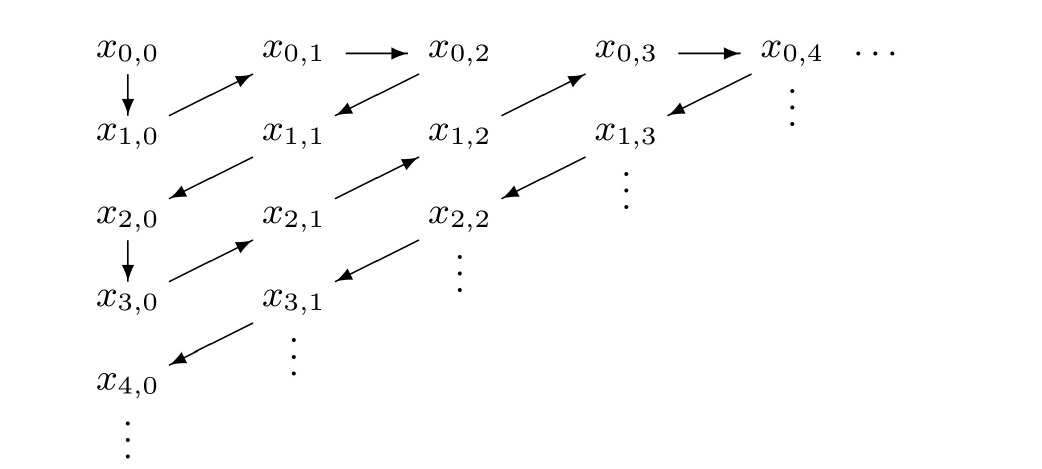
\includegraphics[width=0.78\textwidth]{figures/d1a18a5464e9cd86.jpg}
\end{equation}

我们把明确写出这个双射的任务留给读者。■

\end{proposition}

\begin{proposition}

可数集的有限积是可数的。

\proofhead
设 $X_j, j = 0, 1, \ldots, n$ 是可数集，$X := \prod_{j=0}^{n} X_j$。按定义 $X = (\prod_{j=0}^{n-1} X_j) \times X_n$，故只需考虑 $n = 1$ 的情形。于是设 $X := X_0 \times X_1$，其中 $X_0$ 与 $X_1$ 可数无限。记 $X_0 = \{ y_k : k \in \mathbb{N} \}$，$X_1 = \{ z_k : k \in \mathbb{N} \}$，并对 $j, k \in \mathbb{N}$ 令 $x_{j,k} := (y_j, z_k)$。采用这一记号便有 $X = \{ x_{j,k} : j, k \in \mathbb{N} \}$，因此我们可以再次用 (6.3) 定义从 $X$ 到 $\mathbb{N}$ 的双射。
\end{proposition}

\subsection*{无限积}

若允许可数集的“无限积”，命题 6.9 就不再正确。为使这一说法更精确，我们需要先解释什么是“无限积”。设 $ \{X_\alpha; \alpha \in \mathbb{A}\} $ 是一个固定集合的子集族。则笛卡儿积 $ \prod_{\alpha \in \mathbb{A}} X_\alpha $ 定义为所有这样的函数构成的集合：

$ \varphi: A \to \bigcup_{\alpha \in A} X_\alpha $ 使得对每个 $ \alpha \in A $ 有 $ \varphi(\alpha) \in X_\alpha $。人们常用 $ \{x_\alpha; \alpha \in \mathsf{A}\} $ 代替 $ \varphi $，其中当然 $ x_\alpha := \varphi(\alpha) $。

在特殊情形 $ \mathbf{A} = \{1, \ldots, n\} $（其中 $ n \in \mathbb{N}^\times $）下，$ \prod_{\alpha \in \mathbb{A}} X_\alpha $ 显然与第 2 节引入的积 $ \prod_{k=1}^{n} X_k $ 相同。若对每个 $ \alpha \in \mathbb{A} $ 都有 $ X_\alpha = X $，则记 $ X^{\mathbb{A}} := \prod_{\alpha \in \mathbb{A}} X_\alpha $。

\begin{remark}

显然，若诸 $ X_\alpha $ 中有一个（或更多）是空集，则 $ \prod_{\alpha \in \mathcal{A}} X_\alpha = \emptyset $。另一方面，即使对每个 $ \alpha \in \mathcal{A} $ 都有 $ X_\alpha \neq \emptyset $，用我们迄今所见过的集合论公理也无法证明 $ \prod_{\alpha \in \mathcal{A}} X_\alpha $ 非空。为此需要知道存在函数 $ \varphi: \mathcal{A} \to \bigcup_{\alpha \in \mathcal{A}} X_\alpha $，使得对每个 $ \alpha \in \mathcal{A} $ 有 $ \varphi(\alpha) \in X_\alpha $，即存在一条从每个集合 $ X_\alpha $ 中选出一个元素的规则。为确保这样的函数存在，需要选择公理，我们把它表述如下：对任意集族 $ \{X_\alpha : \alpha \in \mathcal{A}\} $，

\[
\prod_{\alpha\in A}X_{\alpha}\neq\emptyset\Longleftrightarrow(X_{\alpha}\neq\emptyset\;\;\forall\alpha\in\mathsf{A})~.
\]

以下我们将不加说明地使用这一自然出现的公理。对数学基础感兴趣的读者可参阅文献，例如 [Ebb77] 和 [FP85]。■

令人惊讶的是，与命题 6.9 相反，有限集的可数无限积一般不是可数的，如下面的命题所示。

\end{remark}

\begin{proposition}

集合 $ \{0,1\}^{\mathbb{N}} $ 是不可数的。

\proofhead
设 $ A \in \mathcal{P}(\mathbb{N}) $。则特征函数 $ \chi_A $ 是 $ \{0,1\}^{\mathbb{N}} $ 的一个元素。显然函数
\begin{equation}
\mathcal{P}(\mathbb{N})\to\{0,1\}^{\mathbb{N}},\quad A\mapsto\chi_{A}
\end{equation}

是单射。对 $\varphi \in \{0,1\}^{\mathbb{N}}$，令 $A(\varphi):=\varphi^{-1}(1)\in \mathcal{P}(\mathbb{N})$。则 $\chi_{A(\varphi)}=\varphi$。这表明函数 (6.4) 是满射的。（另见习题 3.6。）因此 $\{0,1\}^{\mathbb{N}}$ 与 $\mathcal{P}(\mathbb{N})$ 等势，而结论由推论 6.6 得出。

\end{proposition}

\begin{corollary}

集合 $\{0,1\}^{\mathbb{N}}$ 与 $\mathcal{P}(\mathbb{N})$ 等势。

\end{corollary}

\exerciseshead

\begin{exercises}
\item

设 $ n \in \mathbb{N}^\times $。证明从 $ \{1, \ldots, n\} $ 到自身的任何单射函数都是双射。（提示：对 $ n $ 作归纳。设 $ f: \{1, \ldots, n+1\} \to \{1, \ldots, n+1\} $ 是单射函数，$ k := f(n+1) $。考虑函数

\begin{equation*}
g(j):=\left\{\begin{array}{c l}{n+1\;,}&{\quad j=k\;,}\\ {k\;,}&{\quad j=n+1\;,}\\ {j}&{\quad\text{其他情形},}\\ \end{array}\right.
\end{equation*}

以及 $ h := g \circ f $ 和 $ h | \{1, \ldots, n\} $。）

\item

证明下列各题：

\begin{items}
\item

设 $ m, n \in \mathbb{N}^{\times} $。则存在从 $ \{1, \ldots, m\} $ 到 $ \{1, \ldots, n\} $ 的双射函数当且仅当 $ m = n $。

\item

若 $M$ 是无限系统，则 $\text{Num}(M) = \infty$（提示：习题 1）。

\end{items}

\item

证明 $n$ 元集的 $m$ 元子集的个数是 $\binom{n}{m}$。（提示：设 $N$ 是 $n$ 元集，$M$ 是 $N$ 的 $m$ 元子集。由命题 6.3 推出，有 $m!(n-m)!\; \text{个从} \{1,\ldots,n\} \text{到} N \text{的双射，使得} \{1,\ldots,m\} \text{映到} M.)$

\item

设 M 和 N 是有限集。从 M 到 N 的单射函数有多少个？

\item

设 $ X_0, \ldots, X_m $ 是有限集。证明 $ X := \bigcup_{i=0}^{m} X_j $ 也是有限的，且

\[
Num(X)\leq\sum_{j=0}^{m}Num(X_{j})~.
\]

何时取等号？

\item

设 $ X_0, \ldots, X_m $ 是有限集。证明 $ X := \prod_{i=0}^{m} X_i $ 也是有限的，且

\[
Num(X)=\prod_{j=0}^{m}Num(X_{j})~.
\]
\item

证明非空集合 X 是可数的当且仅当存在从 N 到 X 的满射。

\item

设 $X$ 是可数集。证明 $X$ 的所有有限子集构成的集合是可数的。（提示：考虑函数 $X^n \to \mathcal{E}_n(X)$，$(x_1, \ldots, x_n) \mapsto \{x_1, \ldots, x_n\}$，其中 $\mathcal{E}_n(X)$ 是元素个数至多为 $n$ 的所有子集构成的集合。）

\item

证明有限集的任何子集都是有限的。

\end{exercises}

\section{群与同态}

在定理 5.3 中，当 $ m \leq n $ 时，我们定义了两个自然数 m 与 n 的差 $ n - m $。当 m 是 n 的因子时，我们也定义了两个自然数 m 与 n 的商 n/m。在这两种情形中，对 m 与 n 所加的这些限制都是必需的，以保证差与商仍然是自然数。如果要定义任意自然数 m 与 n 的“差” n - m 或“商” n/m，我们就必须离开自然数的领域。在 9–11 节中，我们将构造新的数，从而把自然数集扩充为更大的数系，在这些数系中这些运算可以（几乎）不受限制地使用。

当然，这些新的数系必须这样构造，使得通常的加法与乘法法则成立。为此，撇开与某一特定数系的联系而考察这些法则本身，是极为有益的。这样的考察也为从定义与公理出发对命题作逻辑推演提供了进一步的练习。

这里以及随后各节所出现问题的深入讨论属于代数而非分析，因此我们的叙述相对简短，只证明少数最重要的定理。我们的目标是能够认出那些以各种伪装反复出现的一般代数结构。从少量公理推导出大量算术法则，将使我们能够为本来庞杂的一堆公式与结果建立秩序，并把注意力保持在本质之处。我们从公理推出的命题，只要公理成立便成立，而与它们成立的具体情境无关。已经证明过一次的东西，无需对每个特殊情形再证明一次。

在本节及随后各节中，我们只给出这些新概念的少数具体例子。我们主要着眼于提供一种语言，并希望读者在后面的各节中能认识到这种语言的用处，同时也能看到形式化背后的数学内容。

\subsection*{群}

群是由一个集合、一个运算和三条公理组成的系统。由于它们具有如此简单的代数结构，因而在数学中处处可见。

由非空集合 G 与一个运算 $ \odot $ 组成的对 $ (G,\odot) $ 称为群，如果下列条件成立：

$ (G_1) $：$ \odot $ 是结合的。

$ (G_{2}) \odot $ 有单位元 e。

$ (G_3) $ 每个 $ g \in G $ 都有一个 $ \mathbf{逆元} $ $ h \in G $，使得 $ g \odot h = h \odot g = e $。

若 $ \odot $ 是 $ G $ 上的交换运算，则群 $ (G, \odot) $ 称为交换群或阿贝尔群。若运算从上下文看是明确的，我们常把 $ (G, \odot) $ 简记为 $ G $。

\begin{remark}

设 $  G = (G, \odot)  $ 是一个群。

\begin{items}
\item

由命题 4.11，单位元 e 是唯一的。

\item

每个 $ g \in G $ 都有唯一的逆元，我们（暂时）把它记为 $ g^b $。特别地 $ e^b = e $。

\proofhead
鉴于 $(G_3)$，只需证明唯一性。设 $h$ 与 $k$ 都是 $g \in G$ 的逆元，即 $g \odot h = h \odot g = e$ 且 $g \odot k = k \odot g = e$。则
\[
h=h\odot e=h\odot(g\odot k)=(h\odot g)\odot k=e\odot k=k,
\]

这就证明了唯一性。
由于 $ e \odot e = e $，第二个断言是显然的。■

\item

对每一对 $a,b\in G$，存在唯一的 $x\in G$ 使 $a\odot x=b$，也存在唯一的 $y\in G$ 使 $y\odot a=b$。也就是说，“方程” $a\odot x=b$ 与 $y\odot a=b$ 有唯一解。

\proofhead
设给定 $a, b \in G$。若令 $x := a^{\flat} \odot b$ 与 $y := b \odot a^{\flat}$，则 $a \odot x = b$ 且 $y \odot a = b$。这证明了存在性。为验证第一个方程解的唯一性，设 $x, z \in G$ 满足 $a \odot x = b$ 且 $a \odot z = b$。则
\[
x=(a^{\flat}\odot a)\odot x=a^{\flat}\odot(a\odot x)=a^{\flat}\odot b=a^{\flat}\odot(a\odot z)=(a^{\flat}\odot a)\odot z=z.
\]

对方程 $ y\odot a=b $ 作类似的论证即完成证明。■

\item

对每个 $ g \in G $，我们有 $ (g^{\flat})^{\flat} = g $。

\proofhead
由逆元的定义直接得到等式
\[
g\odot g^{\flat}=g^{\flat}\odot g=e\;,
\]
\[
\left(g^{\flat}\right)^{\flat}\odot g^{\flat}=g^{\flat}\odot\left(g^{\flat}\right)^{\flat}=e,
\]

它们与 (c) 一起推出 $  g = (g^{\flat})^{\flat}  $。■

\item

设 $H$ 是带有结合运算 $\circledast$ 与单位元 $e$ 的非空集合。若每个元素 $h \in H$ 都有一个 $\text{左} \text{逆} \overline{h}$ 使 $\overline{h} \circledast h = e$，则 $(H, \circledast)$ 是一个群且 $\overline{h} = h^{\flat}$。类似地，若每个元素 $h \in H$ 都有一个 $\text{右} \text{逆} \underline{h}$ 使 $h \circledast \underline{h} = e$，则 $(H, \circledast)$ 是一个群且 $\underline{h} = h^{\flat}$。

\proofhead
设 $h$ 属于 $H$，$\overline{h}$ 是 $h$ 的左逆，且 $\overline{h}$ 是 $\overline{h}$ 的左逆。则 $\overline{\overline{h}} \circledast \overline{h} = e$，于是
\[
h=e\circledast h=\left(\overline{\overline{h}}\circledast\overline{h}\right)\circledast h=\overline{{\overline{{h}}}}~\circledast\left(\overline{{h}}\circledast h\right)=\overline{{\overline{{h}}}}~\circledast e=\overline{{\overline{{h}}}}\;,
\]

由此可得 $ h \circledast \overline{h} = e $。因此 $ \overline{h} $ 也是 $ h $ 的右逆，从而是 $ h $ 的逆。类似地可以证明，若每个元素都有右逆，则每个右逆也是左逆。$ \blacksquare $

\item

对任意的群元素 $ g $ 与 $ h $，$ (g \odot h)^{\flat} = h^{\flat} \odot g^{\flat} $。

\proofhead
由于 $ (h^{\flat}\odot g^{\flat})\odot(g\odot h)=h^{\flat}\odot(g^{\flat}\odot g)\odot h=h^{\flat}\odot e\odot h=h^{\flat}\odot h=e $，该断言由 (e) 推出。■
\end{items}

为了说明一个公理系统是无矛盾的，只需给出某个满足这些公理的数学系统。就群公理 $ (G_{1})-(G_{3}) $ 而言，这相当容易做到，如下面的例子所示。

\end{remark}

\begin{example}

\begin{items}
\item

设 $G := \{e\}$ 是单元素集。则 $\{G, \odot\}$ 是交换群，即\textbf{平凡}群，其（唯一可能的）运算为 $e \odot e = e$。

\item

设 $G := \{a, b\}$ 是带有由右表所定义运算 $\odot$ 的集合。则 $(G, \odot)$ 是交换群。

\item

设 $X$ 是非空集合，$S_X$ 是从 $X$ 到自身的所有双射的集合。当 $\circ$ 表示函数的复合时，$S_X := (S_X, \circ)$ 是一个以 $id_X$ 为单位元的群。此外，反函数 $f^{-1}$ 就是 $f \in S_X$ 在该群中的逆。由习题 4.3，$S_X$ 一般不是交换的。当 $X$ 有限时，$S_X$ 的元素称为置换（见 6 节），$S_X$ 称为 $X$ 的置换群。

\end{items}

\begin{center}
\begin{tabular}{ccc}
\toprule
$ \odot $ & a & b \\
a & a & b \\
b & b & a \\
\bottomrule
\end{tabular}
\end{center}

\begin{items}
\item[（d）]

设 $X$ 是非空集合，$(G, \odot)$ 是一个群。以如例 4.12 中那样的诱导运算 $\odot$，$(G^X, \odot)$ 是一个群。$f \in G^X$ 的逆是函数

\[
f^{\flat}\colon X\to G~,\quad x\mapsto\left(f(x)\right)^{\flat}~.
\]

特别地，当 $ m \geq 2 $ 时，带有运算

\[
(g_{1},\cdots,g_{m})\odot(h_{1},\cdots,h_{m})=(g_{1}\odot h_{1},\cdots,g_{m}\odot h_{m})
\]

的 $ G^m $ 是一个群。

\item[（e）]

设 $ G_1, \ldots, G_m $ 是群。则带有与 (d) 类似地定义的运算的 $ G_1 \times \cdots \times G_m $ 是一个群，称为 $ G_1, \ldots, G_m $ 的直积。■

\end{items}

\end{example}

\subsection*{子群}

设 $ G = (G, \odot) $ 是一个群，$ H $ 是 $ G $ 的非空子集，且对运算 $ \odot $ 封闭，即

$ (\mathrm{SG}_1) $ $ H \odot H \subseteq H $.

若此外还有

(SG$_2$) 对一切 $ h \in H $ 都有 $ h^{\flat} \in H $，

则 $H := (H, \odot)$ 本身也是一个群，称为 $G$ 的子群。这里我们用同一符号 $\odot$ 表示运算在 $H$ 上的限制。由于 $H$ 非空，存在某个 $h \in H$，于是由 $(SG_1)$ 与 $(SG_2)$，$e = h^b \odot h$ 也在 $H$ 中。

\begin{example}

设 $  G = (G, \odot)  $ 是一个群。

\begin{items}
\item

平凡子群 $ \{e\} $ 与 G 本身都是 G 的子群，它们分别是关于包含关系的最小与最大子群（见例 4.4.(b)）。

\item

若 $ H_\alpha $，$ \alpha \in \mathsf{A} $ 是 $ G $ 的子群，则 $ \bigcap_\alpha H_\alpha $ 也是 $ G $ 的子群。■

\end{items}

\end{example}

\subsection*{陪集}

设 $N$ 是 $G$ 的子群，$g \in G$。则 $g \odot N$ 是 $g \in G$ 关于 $N$ 的左陪集，$N \odot g$ 是右陪集。若我们定义

\begin{equation}
g\sim h:\Leftrightarrow g\in h\odot N,
\end{equation}

则 $\sim$ 是 $G$ 上的等价关系：事实上，由于 $e \in N$，$\sim$ 是自反的。若 $g \in h \odot N$ 且 $h \in k \odot N$，则

\[
g\in\left(k\odot N\right)\odot N=k\odot\left(N\odot N\right)=k\odot N~,
\]

因为，当然。

\begin{equation}
N\odot N=N.
\end{equation}

因此 $\sim$ 是传递的。若 $g \in h \odot N$，则存在某个 $n \in N$ 使 $g = h \odot n$。于是由 (SG$_{2}$) 可得 $h = g \odot n^{\flat} \in g \odot N$。因此 $\sim$ 也是对称的，且 (7.1) 定义了 $G$ 上的一个等价关系。对于关于 $\sim$ 的等价类 $[ \cdot ]$，我们有

\begin{equation}
[g]=g\odot N~,\qquad g\in G~.
\end{equation}

因此，我们把 $ G/\sim $ 记为 G/N，并称 G/N 为 G 模 N 的左陪集集合。

特别重要的是满足下式的子群 N：

\begin{equation}
g\odot N=N\odot g~,\qquad g\in G~.
\end{equation}

这样的子群称为 $G$ 的\textbf{正规}子群。此时称 $g\odot N$ 为 $g$ \textbf{模} $N$ 的\textbf{陪集}，因为每个左陪集都是右陪集，反之亦然。

对于 G 的正规子群 N，由 (7.2)、(7.4) 以及运算的结合性可得

\[
(g\odot N)\odot(h\odot N)=g\odot(N\odot h)\odot N=(g\odot h)\odot N~,\qquad g,h,\in G~.
\]

这表明在 $G/N$ 上存在一个由 $\odot$ 诱导的良定义运算，使得

\begin{equation}
(G/N)\times(G/N)\to G/N~,\quad(g\odot N,h\odot N)\mapsto(g\odot h)\odot N~.
\end{equation}

我们将用同一符号 $ \odot $ 表示这个诱导运算。

\begin{proposition}

设 G 是一个群，N 是 G 的正规子群。则带有诱导运算的 G/N 是一个群，称为 G 模 N 的商群。

\proofhead
读者容易验证诱导运算是结合的。由于 $(e\odot N)\odot(g\odot N)=(e\odot g)\odot N=g\odot N$，$G/N$ 的单位元是 $N=e\odot N$。又由于
\[
(g^{\flat}\odot N)\odot(g\odot N)=(g^{\flat}\odot g)\odot N=e\odot N=N
\]

由注 7.1(e) 可得该断言。■

\end{proposition}

\begin{remark}

\begin{items}
\item

在 (7.3) 的记号下，[e] = N 是 $G/N$ 的单位元，$[g]^{\flat}$ = $[g^{\flat}]$ 是 [g] ∈ $G/N$ 的逆元。由 (7.3) 与 (7.5) 我们有

\[
[g]\odot[h]=[g\odot h]~,\qquad g,h\in G~.
\]

换句话说，要用运算 $ \odot $ 合并两个陪集，可以各取每个陪集的一个代表元，用 $ \odot $ 合并这些元素，然后取包含所得元素的陪集。由于 $ G/N $ 上的运算是良定义的，最终结果与代表元的具体选取无关。

\item

阿贝尔群 $G$ 的任何子群 $N$ 都是正规的，因此 $G/N$ 是一个群。当然，$G/N$ 也是阿贝尔群。

\end{items}

\end{remark}

\subsection*{同态}

在群之间的函数中，那些保持群结构的函数特别重要。

设 $ G = (G, \odot) $ 与 $ G' = (G', \circledast) $ 是群。函数 $ \varphi: G \to G' $ 称为（群）同态，如果

\[
\varphi(g\odot h)=\varphi(g)\circledast\varphi(h)~,\qquad g,h\in G~.
\]

从 G 到自身的同态称为（群）自同态。

\begin{remark}

\begin{items}
\item

设 e 与 $ e' $ 分别是 G 与 $ G' $ 的单位元，并设 $ \varphi: G \to G' $ 是一个同态。则

\[
\varphi(e)=e^{\prime}\quad\text{且}\quad\left(\varphi(g)\right)^{\flat}=\varphi(g^{\flat}),\qquad g\in G.
\]

\proofhead
由 $e'\circledast\varphi(e)=\varphi(e)=\varphi(e\odot e)=\varphi(e)\circledast\varphi(e)$ 与注 7.1(c) 可得 $\varphi(e)=e^{\prime}$。设 $g\in G$。则 $e^{\prime}=\varphi(e)=\varphi(g^{\flat}\odot g)=\varphi(g^{\flat})\circledast\varphi(g)$，类似地 $e^{\prime}=\varphi(g)\circledast\varphi(g^{\flat})$。于是由注 7.1(b) 得 $\left(\varphi(g)\right)^{\flat}=\varphi(g^{\flat})$。
\item

设 $ \varphi: G \to G' $ 是一个同态。$ \varphi $ 的核 $ \ker(\varphi) $ 定义为

\[
\ker(\varphi):=\varphi^{-1}(e^{\prime})=\left\{g\in G\;;\;\varphi(g)=e^{\prime}\right\}\;,
\]

是 G 的正规子群。

\proofhead
对一切 $ g, h \in \ker(\varphi) $ 我们有
\[
\varphi(g\odot h)=\varphi(g)\circledast\varphi(h)=e^{\prime}\circledast e^{\prime}=e^{\prime}\;.
\]

因此 (SG$_1$) 满足。由于 $ \varphi(g^{\flat}) = (\varphi(g))^{\flat} = (e')^{\flat} = e' $，(SG$_2$) 也成立，所以 $ \ker(\varphi) $ 是 $ G $ 的子群。设 $ h \in g \odot \ker(\varphi) $。则存在某个 $ n \in G $ 使 $ \varphi(n) = e' $ 且 $ h = g \odot n $。对 $ m := g \odot n \odot g^{\flat} $，我们有

\[
\varphi(m)=\varphi(g)\circledast\varphi(n)\circledast\varphi(g^{\flat})=\varphi(g)\circledast\varphi(g^{\flat})=e^{\prime}~,
\]

从而 $ m \in \ker(\varphi) $。由于 $ m \odot g = g \odot n = h $，这意味着 $ h \in \ker(\varphi) \odot g $。类似地可以证明 $ \ker(\varphi) \odot g \subseteq g \odot \ker(\varphi) $，于是 $ \ker(\varphi) $ 是 $ G $ 的正规子群。$ \blacksquare $

\item

设 $ \varphi: G \to G' $ 是一个同态，$ N := \ker(\varphi) $。则

\[
g\odot N=\varphi^{-1}\bigl(\varphi(g)\bigr),\qquad\quad g\in G,
\]

从而

\[
g\sim h\Longleftrightarrow\varphi(g)=\varphi(h)~,\qquad g,h\in G~,
\]

其中 $ \sim $ 表示等价关系 (7.1)。

\proofhead
对 $ h \in g \odot N $ 我们有
\[
\varphi(h)\in\varphi(g\odot N)=\varphi(g)\circledast\varphi(N)=\varphi(g)\circledast\{e^{\prime}\}=\left\{\varphi(g)\right\},
\]

从而 $ h \in \varphi^{-1}(\varphi(g)) $。反之，若 $ h \in \varphi^{-1}(\varphi(g)) $，即 $ \varphi(h) = \varphi(g) $，则

\[
\varphi(g^{\flat}\odot h)=\varphi(g^{\flat})\circledast\varphi(h)=\left(\varphi(g)\right)^{\flat}\circledast\varphi(g)=e^{\prime}~,
\]

这意味着 $ g^{\flat} \odot h \in N $，从而 $ h \in g \odot N $。■

\item

一个同态是单射当且仅当它的核是平凡的，即 $ \ker(\varphi) = \{e\} $。

\proofhead
这直接由 (c) 推出。
\item

同态 $ \varphi: G \to G' $ 的像 $ \mathrm{im}(\varphi) $ 是 $ G' $ 的子群。■

\end{items}

\end{remark}

\begin{example}

\begin{items}
\item

常值函数 $ G \to G' $，$ g \mapsto e' $ 是同态，即平凡同态。

\item

恒等函数 $ \mathrm{id}_{G}: G \to G $ 是自同态。

\item

同态（自同态）的复合是同态（自同态）。

\item

设 N 是 G 的正规子群。则商函数

\[
p\colon G\to G/N~,\quad g\mapsto g\odot N
\]

是满同态，称为商同态，且 $ \ker(p) = N $。

\proofhead
由于 $N$ 是 $G$ 的正规子群，商群 $G/N$ 是良定义的。由 (7.1) 与命题 4.1，商函数 $p$ 是良定义的，且注 7.5(a) 表明 $p$ 是同态。由于 $N$ 是 $G/N$ 的单位元，$\ker(p)=N$。
\item

若 $ \varphi: G \to G' $ 是双射同态，则 $ \varphi^{-1}: G' \to G $ 也是。■

\end{items}

\end{example}

\subsection*{同构}

若 $\varphi$ 是双射，则同态 $\varphi: G \to G'$ 称为从 $G$ 到 $G'$ 的（群）同构。在此情形下，我们说群 $G$ 与 $G'$ 同构，并记作 $G \cong G'$。从 $G$ 到自身的同构，即双射自同态，称为 $G$ 的（群）自同构。

\begin{example}

\begin{items}
\item

恒等函数 $\mathrm{id}_{G}: G \to G$ 是自同构。若 $\varphi$ 与 $\psi$ 是 $G$ 的自同构，则 $\varphi \circ \psi$ 与 $\varphi^{-1}$ 也是。由此容易推出，群 $G$ 的所有自同构组成的集合以复合为运算构成一个群，称为 $G$ 的自同构群。它是置换群 $S_{G}$ 的子群。

\item

对每个 $ a \in G $，函数 $ g \mapsto a \odot g \odot a^{\flat} $ 是 $ G $ 的自同构。

\item

设 $ \varphi: G \to G' $ 是一个同态。则存在唯一的单射同态 $ \widetilde{\varphi}: G/\ker(\varphi) \to G' $，使得图

\[
\begin{tikzcd}[row sep=2.6em, column sep=3.6em]
G \arrow[r, "\varphi"] \arrow[d, "p"'] & G' \\
G/\ker(\varphi) \arrow[ur, "\widetilde{\varphi}"]
\end{tikzcd}
\]

交换。若 $ \varphi $ 是满射，则 $ \widetilde{\varphi} $ 是同构。

\proofhead
由注 7.6(c) 与例 4.2(c) 可得，存在唯一的单射函数 $ \widetilde{\varphi} $ 使图交换，且 $ \mathrm{im}(\varphi) = \mathrm{im}(\widetilde{\varphi}) $。容易验证 $ \widetilde{\varphi} $ 是同态。
\item

设 $ (G, \odot) $ 是一个群，$ G' $ 是非空集合，$ \varphi: G \to G' $ 是从 $ G $ 到 $ G' $ 的双射。在 $ G' $ 上定义运算 $ \circledast $ 为

\[
g^{\prime}\circledast h^{\prime}:=\varphi^{-1}(g^{\prime})\odot\varphi^{-1}(h^{\prime}),\qquad g^{\prime},h^{\prime}\in G^{\prime}.
\]

则 $ (G', \circledast) $ 是一个群，且 $ \varphi $ 是从 $ G $ 到 $ G' $ 的同构。运算 $ \circledast $ 称为 $ G' $ 上由 $ \varphi $ 从 $ \circledast $ 诱导的运算。

\item

若 $ G = \{e\} $ 与 $ G' = \{e'\} $ 是平凡群，则 G 与 $ G' $ 同构。

\item

设 $G$ 是例 7.2(b) 中的群，$G'$ 是把表中的符号 $a$ 与 $b$ 互换后所得的群。则 $G$ 与 $G'$ 同构。更确切地说，$G'$ 上的运算是由函数 $\varphi: \{a, b\} \to \{a, b\}$（由 $\varphi(a) := b$ 与 $\varphi(b) := a$ 定义）从运算 $G$ 诱导的。

\item

设 X 与 Y 是非空集合，$ \varphi: X \to Y $ 是双射函数。则

\[
\widehat{\varphi}\colon\mathsf{S}_{X}\to\mathsf{S}_{Y}~,\quad f\mapsto\varphi\circ f\circ\varphi^{-1}
\]

是从置换群 $S_X$ 到置换群 $S_Y$ 的同构。■

\end{items}

若 $\varphi$ 是从群 $(G, \odot)$ 到群 $(G', \circ)$ 的同构，那么即使这两个群在元素的记号上可能不同，它们也具有相同的群结构。例如，若 $g$ 与 $h$ 是 $G$ 的两个元素，那么要计算 $g \odot h$，也同样可以在 $G'$ 中计算 $\varphi(g) \otimes \varphi(h)$，然后 $g \odot h$ 就是 $\varphi(g) \otimes \varphi(h)$ 在逆同构 $\varphi^{-1}$ 下的像。实际上，与 $(G', \circ)$ 打交道可能比与 $(G, \odot)$ 容易得多。（特别参见 9 节与 10 节。）

从群论的观点看，同构的群本质上是相同的。事实上，同构 $ \cong $ 是任何群集 $ \mathcal{G} $ 上的等价关系，这容易验证。因此可以用 $ \cong $ 把 $ \mathcal{G} $ 划分为等价类，称为同构类。于是只需研究同构类的集合 $ \mathcal{G}/\cong $，而不必研究 $ \mathcal{G} $ 本身。换句话说，人们把同构的群“等同”（视为相同）。正是在这个意义上，人们谈论平凡群，因为由例 7.8(e)，任何两个平凡群都同构。类似地，阶为\footnote{有限群的阶是其元素的个数。} 2 的群，即恰有两个元素的群，在同构意义下只有一个（见例 7.8(f)）。若 $ n \in \mathbb{N}^\times $，则由例 7.8(g)，只需考虑一个满足 $ \text{Num}(X) = n $ 的置换群 $ S_X $，例如阶为 $ n! $ 的置换群（或对称群），

\[
\mathsf{S}_{n}:=\mathsf{S}_{\{1,\ldots,n\}},
\]

即集合 $ \{1,\ldots,n\} $ 上的置换群。（见命题 6.3。）

约定 在下文中，我们通常把群 $G$ 中的运算记为 $\cdot$，并且对 $x, y \in G$，不写 $x \cdot y$ 而简写为 $xy$。采用这种“乘法”记号时，该运算称为（群）乘法，而 $x^{\flat}$ 写作 $x^{-1}$（“$x$ 的逆”）。若群是阿贝尔群，通常使用“加法记号”，即群运算写作 + 并称为加法，$x$ 的逆 $x^{\flat}$ 写作 $-x$（“负 $x$”）。

再次提醒读者，记号并不重要，重要的是公理。同一符号在不同的

情境中可以具有完全不同的含义，即使适用的公理相同。使用诸如 + 或 $ \cdot $ 这类熟悉的符号，不应使读者以为所指的是熟悉的情境。必须清楚哪些公理在起作用，并只使用由它们推出的规则。

同一个符号可以有各种依赖情境的含义，这在初学者看来也许不合逻辑、令人困惑。尽管如此，它使得复杂思想能够以优雅而简洁的方式得到表述，并避免用大量不同符号使读者不堪重负。

\end{example}

\exerciseshead

\begin{exercises}
\item

设 $N$ 是有限群 $G$ 的子群。证明 $\text{Num}(G) = \text{Num}(N) \cdot \text{Num}(G/N)$，从而特别地，子群的阶整除群的阶。

\item

验证例 7.2(c) 与 (d) 中的断言。

\item

证明例 7.3(b) 中的断言，并证明一组正规子群的交也是正规的。

\item

证明注 7.6(e)。$ \operatorname{im}(\varphi) $ 是 $ G' $ 的正规子群吗？

\item

设 $ \varphi: G \to G' $ 是一个同态，$ N' $ 是 $ G' $ 的正规子群。证明 $ \varphi^{-1}(N') $ 是 G 的正规子群。

\item

设 G 是一个群，X 是非空集合。则称 G（从左）作用在 X 上，若存在一个函数

\[
G\times X\to X~,\quad(g,x)\mapsto g\cdot x
\]

使得下列条件成立：

$ (GA_1)\;e \cdot x = x $ 对一切 $ x \in X $ 成立。

$ (GA_2)\;g\cdot(h\cdot x)=(gh)\cdot x $ 对一切 $ g,h\in G $ 与 $ x\in X $ 成立

\begin{items}
\item

对每个 $g \in G$，证明 $x \mapsto g \cdot x$ 是 $X$ 上的双射，其逆为 $x \mapsto g^{-1} \cdot x$。

\item

对 $ x \in X $，$ G \cdot x $ 称为 $ x $ 的\textbf{轨道}（在 $ G $ 的作用下）。证明关系“$ y $ 在 $ x $ 的轨道中”是 $ X $ 上的等价关系。

\item

证明若 $H$ 是 $G$ 的子群，则 $(h,g) \mapsto h \cdot g$ 与 $(h,g) \mapsto hgh^{-1}$ 定义了 $H$ 在 $G$ 上的作用。

\item

证明

\[
{\sf S}_{m}\times{\mathbb{N}}^{m}\to{\mathbb{N}}^{m},\quad(\sigma,\alpha)\mapsto\sigma\cdot\alpha:=(\alpha_{\sigma(1)},\ldots,\alpha_{\sigma(m)})
\]

定义了 $ S_{m} $ 在 $ N^{m} $ 上的作用。

\end{items}

\item

设 $ G = (G, \odot) $ 是阶为 $ m $、单位元为 $ e $ 的有限群。证明对每个 $ g \in G $，存在最小的自然数 $ k > 0 $ 使得

\[
g^{k}:=\bigodot_{j=1}^{k}g=e.
\]

证明对一切 $ g \in G $ 都有 $ g^m = e $。（提示：习题 1。）

\item

下面的表在集合 $ G = \{e, a, b, c\} $ 上定义了三个运算

\begin{center}
\begin{tabular}{ccccc}
\toprule
$ \odot $ & e & a & b & c \\
e & e & a & b & c \\
a & a & e & c & b \\
b & b & c & e & a \\
c & c & b & a & e \\
\bottomrule
\end{tabular}
\end{center}

\begin{center}
\begin{tabular}{ccccc}
\toprule
$ \circledast $ & e & a & b & c \\
e & e & a & b & c \\
a & a & e & c & b \\
b & b & c & a & e \\
c & c & b & e & a \\
\bottomrule
\end{tabular}
\end{center}

\begin{center}
\begin{tabular}{ccccc}
\toprule
$ \oplus $ & e & a & b & c \\
e & e & a & b & c \\
a & a & b & c & e \\
b & b & c & e & a \\
c & c & e & a & b \\
\bottomrule
\end{tabular}
\end{center}

\begin{items}
\item

验证 $ (G, \circledast) $ 与 $ (G, \oplus) $ 是同构的群。

\item

证明群 $ (G,\odot) $ 与 $ (G,\circledast) $ 不同构。

\item

确定 G 上所有其他可能的群结构。把这些群按同构类分类。

\end{items}

\item

证明 $ S_{3} $ 不是阿贝尔群。

\item

设 G 与 H 是群，并设

\[
p:G\times H\to G~,\quad(g,h)\mapsto g
\]

是到第一个因子的投影。证明 $p$ 是满同态。

令 $H' := \ker(p)$。证明 $(G \times H)/H'$ 与 $G$ 是同构的群。

\item

设 $G$ 是带有运算 $\odot$ 与单位元的集合。对 $g \in G$，定义函数 $Lg: G \to G$，$h \mapsto g \odot h$，称为由 $g$ 给出的左平移。假设

\[
L:=\left\{Lg\;;\;g\in G\right\}\subseteq{\sf S}_{G}~,
\]

即每个 Lg 都是双射。证明

\[
(G,\odot)\text{ 是群 }\Longleftrightarrow L\text{ 是 }\mathsf{S}_{G}\text{ 的子群 }
\]
\end{exercises}

\section{环、域与多项式}

本节我们考虑定义了两种运算的集合。这里我们假定，就其中一种运算而言，该集合构成一个阿贝尔群，并且这两种运算满足适当的“分配律”。由此引出“环”和“域”的概念，它们把算术规则形式化。作为环的特别重要的例子，我们考虑幂级数环以及一个（和多个）未定元的多项式环，并推导它们的一些基本性质。多项式函数相对容易处理，而且在分析中很重要，因为“复杂的函数可以被多项式任意好地逼近”，这一断言我们稍后会说得更精确。

\subsection*{环}

由非空集合  $ R $ 以及两种运算——加法 + 与乘法  $ \cdot $——组成的三元组  $ (R, +, \cdot) $ 称为环，如果：

$ (R_{1}) $  $ (R,+) $ 是阿贝尔群。

(R\_\{2\}) 乘法是结合的。

(R\_\{3\}) 分配律成立：

\[
(a+b)\cdot c=a\cdot c+b\cdot c,\quad c\cdot(a+b)=c\cdot a+c\cdot b,\qquad a,b,c\in R.
\]

这里我们采用通常的约定，即乘法优先于加法。例如， $ a \cdot b + c $ 表示  $ (a \cdot b) + c $（先做乘法  $ d := a \cdot b $，再做加法  $ d + c $），而不是  $ a \cdot (b + c) $。此外，我们通常把  $ a \cdot b $ 写成  $ ab $。

若乘法是交换的，则称一个环为 \textbf{交换环}。此时，分配律  $ (R_{3}) $ 化为

\begin{equation}
(a+b)c=ac+bc~,\qquad a,b,c\in R~.
\end{equation}

若关于乘法存在单位元，则把它记作  $ 1_R $ 或简记为 1，并称为  $ R $ 的单位元（或乘法单位元），此时我们说  $ (R, +, \cdot) $ 是带单位元的环。当加法与乘法运算由上下文清楚可知时，我们只写  $ R $ 而不写  $ (R, +, \cdot) $。

\begin{remark}

设  $ R := (R, +, \cdot) $ 是一个环。

\begin{items}
\item

环  $ R $ 的加法群  $ (R, +) $ 的单位元，如例 5.14 那样记作  $ 0_R $，或简记为 0，并称为环  $ R $ 的零元（或加法单位元）。由命题 4.11， $ 0_R $ 以及  $ 1_R $（若存在）都是唯一的。

\item

由注 7.1(d) 可得，对每个  $ a \in R $ 都有  $ -(-a) = a $。

\item

对每一对 $a, b \in R$，由注 7.1(c)，方程 $a + x = b$ 有唯一解 $x \in R$，即 $x = b + (-a) =: b - a$（“$b$ 减 $a$”），称为 $a$ 与 $b$ 的差。

\item

对一切  $ a \in R $，都有 0a = a0 = 0 与 -0 = 0。若  $ a \neq 0 $ 且存在某个  $ b \neq 0 $ 使 ab = 0 或 ba = 0，则称 a 为 R 的零因子。若 R 是交换环且没有零因子，即由 ab = 0 可推出 a = 0 或 b = 0，则称 R 为整环。

\proofhead
由于 $0=0+0$，我们有 $a0=a(0+0)=a0+a0$。于是由 (c) 与等式 $a0+0=a0$ 可得 $a0=0$。同理可证 $0a=0$。第二个断言也由 (c) 得到。
\item

对一切 $a, b \in R$，都有 $a(-b) = (-a)b = -(ab) =: -ab$ 与 $(-a)(-b) = ab$。

\proofhead
由 $0 = b + (-b)$ 及 (d) 得 $0 = a0 = ab + a(-b)$。因此，正如上面那样，$a(-b) = -ab$。同理可证 $(-a)b = -ab$。两次使用这一事实可得
\[
(-a)(-b)=-\left(a(-b)\right)=-(-ab)=ab,
\]

其中最后一个等号由 (b) 得到。■

\item

若 $R$ 是带单位元的环，则对一切 $a \in R$ 都有 $(-1)a = -a$。

\proofhead
这是 (e) 的特殊情形。■
\item

由例 5.14(a)，对一切  $ n \in \mathbb{N} $ 与  $ a \in R $， $ n \cdot a = na $ 都有定义，且该例中的规则成立。特别地， $ 0_{\mathbb{N}} \cdot a := 0_R $。由 (d) 我们还有  $ 0_R \cdot a := 0_R $，因此略去  $ 0_{\mathbb{N}} $ 与  $ 0_R $ 的下标不会导致歧义。类似地，若  $ R $ 是带单位元的环，则  $ 1_{\mathbb{N}} \cdot a = 1_R \cdot a = a $。

\end{items}

\end{remark}

\begin{example}

\begin{items}
\item

平凡环恰好只有一个元素 0，它本身也记作 0。含有多于一个元素的环称为非平凡的。平凡环显然是交换的，并且有单位元。若 $R$ 是带单位元的环，则由对每个 $a \in R$ 都有 $1_R \cdot a = a$ 可得，$R$ 是平凡的当且仅当 $1_R = 0_R$。

\item

设  $ R := (R, +, \cdot) $ 是环，X 是非空集合。则  $ R^X $ 关于运算

\[
(f+g)(x):=f(x)+g(x)~,\quad(f g)(x):=f(x)g(x)~,\qquad x\in X~,\quad f,g\in R^{X}~.
\]

构成环。若 $R$ 是交换环（带单位元的环），则 $R^X := (R^X, +, \cdot)$ 也是（见例 4.12）。特别地，对 $m \geq 2$，环 $R$ 的直积 $R^m$ 关于运算

\[
(a_{1},\cdots,a_{m})+(b_{1},\cdots,b_{m})=(a_{1}+b_{1},\cdots,a_{m}+b_{m})
\]

以及

\[
(a_{1},\ldots,a_{m})(b_{1},\ldots,b_{m})=(a_{1}b_{1},\ldots,a_{m}b_{m})
\]

构成一个环，称为积环。若 $R$ 是非平凡的带单位元的环，且 $X$ 至少含有两个元素，则 $R^X$ 有零因子。

\proofhead
第一个断言见例 4.12。对第二个断言，设  $ x, y \in X $ 满足  $ x \neq y $，而  $ f, g \in R^X $ 满足  $ f(x) = 1 $ 以及对一切  $ x' \in X \setminus \{x\} $ 有  $ f(x') = 0 $，又满足  $ g(y) = 1 $ 以及对一切  $ y' \in X \setminus \{y\} $ 有  $ g(y') = 0 $。则  $ fg = 0 $。
\item

设 R 是环，S 是 R 的非空子集，且满足以下条件：
 $ (SR_{1}) $ S 是  $ (R, +) $ 的子群。

\[
(\mathrm{S R}_{2})\setminus S\cdot S\subseteq S.
\]

则 $S$ 本身是一个环，即 $R$ 的子环，而 $R$ 称为 $S$ 的扩环。显然，$0 = \{0\}$ 与 $R$ 都是 $R$ 的子环。即使 $R$ 是带单位元的环，$S$ 也未必如此（见 (e)）。即便如此，若 $1_R \in S$，则 $1_R$ 是 $S$ 的单位元。当然，若 $R$ 是交换环，则 $S$ 也是。反之一般不成立。

\item

子环的交是子环。

\item

设  $ R $ 是非平凡的带单位元的环， $ S $ 是所有这样的  $ g \in R^{\mathbb{N}} $ 的集合：对 \textbf{几乎} 所有（即除有限多个之外的一切） $ n \in \mathbb{N} $ 都有  $ g(n) = 0 $。则  $ S $ 是  $ R^{\mathbb{N}} $ 的无单位元的子环。（为什么？）

\item

设 $X$ 是一个集合。对 $X$ 的子集 $A$ 与 $B$，用下式定义它们的对称差 $A \triangle B$：

\[
A\triangle B:=(A\cup B)\backslash(A\cap B)=(A\backslash B)\cup(B\backslash A).
\]

则  $ (\mathcal{P}(X), \triangle, \cap) $ 是带单位元的交换环。■

\end{items}

设 $R$ 与 $R'$ 是环。一个（环）同态是函数 $\varphi: R \to R'$，它与环的运算相容，即

\begin{equation}
\varphi(a+b)=\varphi(a)+\varphi(b)~,\quad\varphi(ab)=\varphi(a)\varphi(b)~,\qquad a,b\in R~.
\end{equation}

此外，若  $ \varphi $ 是双射，则称  $ \varphi $ 为（环）同构，并称 R 与  $ R' $ 同构。

从  $ R $ 到自身的同态  $ \varphi $ 称为（环）自同态。若  $ \varphi $ 是同构，则称它为（环）自同构。\footnote{当上下文清楚地表明所指的是哪一类同态——群、环（以及后来的域、向量空间或代数）——时，我们将使用“同态”“同构”“自同态”等词。}

\end{example}

\begin{remark}

\begin{items}
\item

环同态  $ \varphi: R \to R' $ 特别地是从  $ (R, +) $ 到  $ (R', +) $ 的群同态。 $ \varphi $ 的核  $ \ker(\varphi) $ 定义为这个群同态的核，即

\[
\ker(\varphi)=\left\{a\in R;\;\varphi(a)=0\right\}=\varphi^{-1}(0).
\]
\item

零函数  $ R \to R' $， $ a \mapsto 0_{R'} $ 是同态，且  $ \ker(\varphi) = R $。

\item

设 $R$ 与 $R'$ 是带单位元的环，$\varphi: R \to R'$ 是同态。如 (b) 所示，不能推出 $\varphi(1_R) = 1_{R'}$。这可看作下述事实的结果：就乘法而言，环不是群。

\end{items}

\end{remark}

\subsection*{二项式定理}

下面我们说明，环公理  $ (R_1)-(R_3) $ 除注 8.1 中的规则外还有其他重要的推论。

\begin{theorem}

（二项式定理） 设 $a$ 与 $b$ 是带单位元的环 $R$ 中两个可交换的元素（即 $ab = ba$）。则对一切 $n \in \mathbb{N}$，

\begin{equation}
(a+b)^{n}=\sum_{k=0}^{n}\binom{n}{k}a^{k}b^{n-k}.
\end{equation}

\proofhead
首先我们注意到，由例 5.14、注 8.1(g) 与习题 5.5，(8.3) 的两端都有定义，且该断言对 $n = 0$ 成立。若 (8.3) 对某个 $n \in \mathbb{N}$ 成立，则
\begin{equation*}
\begin{aligned}
(a+b)^{n+1}&=(a+b)^{n}(a+b)=\biggl(\sum_{k=0}^{n}\binom{n}{k}a^{k} b^{n-k}\biggr)(a+b)\\&=\sum_{k=0}^{n}\binom{n}{k}a^{k+1}b^{n-k}+\sum_{k=0}^{n}\binom{n}{k}a^{k} b^{n+1-k}\\&=a^{n+1}+\sum_{k=0}^{n-1}\binom{n}{k}a^{k+1}b^{n-k}+\sum_{k=1}^{n}\binom{n}{k}a^{k} b^{n+1-k}+b^{n+1}\\&=a^{n+1}+\sum_{k=1}^{n}\biggl\{\binom{n}{k-1}+\binom{n}{k}\biggr\}a^{k} b^{n+1-k}+b^{n+1}.
\end{aligned}
\end{equation*}

由习题 5.5 有  $ \binom{n}{k-1}+\binom{n}{k}=\binom{n+1}{k} $，于是

\[
(a+b)^{n+1}=a^{n+1}+\sum_{k=1}^{n}\binom{n+1}{k}a^{k}b^{n+1-k}+b^{n+1}.
\]

于是由命题 5.7 的归纳原理可得该断言。■

\end{theorem}

\subsection*{多项式定理}

我们希望推广二项式定理，使 (8.3) 的左端允许出现多于两项的和。为使这一公式尽可能简单，引入以下记号是有用的：

对满足  $ m \geq 2 $ 的  $ m \in \mathbb{N} $，元素  $ \alpha = (\alpha_1, \ldots, \alpha_m) \in \mathbb{N}^m $ 称为（$ m $ 阶）多重指标。多重指标  $ \alpha \in \mathbb{N}^m $ 的长度  $ |\alpha| $ 由下式定义

\[
|\alpha|:=\sum_{j=1}^{m}\alpha_{j}.
\]

再令

\[
\alpha!:=\prod_{j=1}^{m}(\alpha_{j})!,
\]

并用下式定义  $ \mathbb{N}^{m} $ 上的自然（偏）序

\[
\alpha\leq\beta:\Leftrightarrow(\alpha_{j}\leq\beta_{j},1\leq j\leq m).
\]

最后，设 $R$ 是带单位元的交换环，$m \in \mathbb{N}$ 且 $m \geq 2$。则我们令

\[
a^{\alpha}:=\prod_{j=1}^{m}(a_{j})^{\alpha_{j}}
\]

其中  $ a = (a_1, \ldots, a_m) \in R^m $， $ \alpha = (\alpha_1, \ldots, \alpha_m) \in \mathbb{N}^m $。

\begin{theorem}

（多项式定理） 设 R 是带单位元的交换环。则对一切  $ m \geq 2 $，

\begin{equation}
\Bigl(\sum_{j=1}^{m}a_{j}\Bigr)^{k}=\sum_{|\alpha|=k}\frac{k!}{\alpha!}a^{\alpha}\;,\qquad a=(a_{1},\ldots,a_{m})\in R^{m}\;,\quad k\in\mathbb{N}\;.
\end{equation}

这里  $ \sum_{|\alpha|=k} $ 是对  $ \mathbb{N}^m $ 中一切长度为  $ k $ 的多重指标求和。

\proofhead
我们先对 m 归纳证明
\begin{equation}
k!/\alpha!\in\mathbb{N}^{\times}\qquad\text{对 }k\in\mathbb{N}\text{ 与 }\alpha\in\mathbb{N}^{m}\text{，}|\alpha|=k.
\end{equation}

先考虑  $ m = 2 $ 的情形。设  $ \alpha \in \mathbb{N}^2 $ 是任意一个长度为  $ k $ 的多重指标。则存在某个满足  $ 0 \leq \ell \leq k $ 的  $ \ell \in \mathbb{N} $ 使  $ \alpha = (\ell, k - \ell) $，于是由习题 5.5(b)，

\[
\frac{k!}{\alpha!}=\frac{k!}{\ell!(k-\ell)!}=\binom{k}{\ell}\in\mathbb{N}^{\times}.
\]

现在设 (8.5) 对某个  $ m \geq 2 $ 成立。任取满足  $ |\alpha| = k $ 的  $ \alpha \in \mathbb{N}^{m+1} $。令  $ \alpha' := (\alpha_2, \ldots, \alpha_{m+1}) \in \mathbb{N}^m $。由归纳假设与习题 5.5(a) 可得

\begin{equation}
\frac{k!}{\alpha!}=\frac{(k-\alpha_{1})!}{\alpha^{\prime}!}\binom{k}{\alpha_{1}}\in\mathbb{N}^{\times}.
\end{equation}

这就完成了归纳以及 (8.5) 的证明。

为证明 (8.4)，我们再次对  $ m $ 归纳。 $ m = 2 $ 的情形就是二项式定理。于是我们假设  $ a = (a_1, \ldots, a_m, a_{m+1}) \in R^{m+1} $（对  $ m \geq 2 $）与

 $ k \in \mathbb{N} $ 是给定的。令  $ b := \sum_{j=2}^{m+1} a_j $，并利用定理 8.4 与归纳假设计算如下：

\begin{equation*}
\begin{aligned}
\Big(\sum_{j=1}^{m+1}a_{j}\Big)^{k}=(a_{1}+b)^{k}&=\sum_{\alpha_{1}=0}^{k}\binom{k}{\alpha_{1}}a_{1}^{\alpha_{1}}b^{k-\alpha_{1}}\\&=\sum_{\alpha_{1}=0}^{k}\binom{k}{\alpha_{1}}a_{1}^{\alpha_{1}}\sum_{|\alpha^{\prime}|=k-\alpha_{1}}\frac{(k-\alpha_{1})!}{\alpha^{\prime}!}a_{2}^{\alpha_{2}}\cdot\cdots\cdot a_{m+1}^{\alpha_{m+1}}\\&=\sum_{\alpha_{1}=0}^{k}\sum_{|\alpha^{\prime}|=k-\alpha_{1}}\frac{(k-\alpha_{1})!}{\alpha^{\prime}!}\binom{k}{\alpha_{1}}a_{1}^{\alpha_{1}}\cdot\cdots\cdot a_{m+1}^{\alpha_{m+1}}\\&=\sum_{|\alpha|=k}\frac{k!}{\alpha!}a^{\alpha},
\end{aligned}
\end{equation*}

其中最后一步我们用了 (8.6)。这就完成了归纳以及定理的证明。

\end{theorem}

\begin{remark}

\begin{items}
\item

多项式系数由下式定义\footnote{我们对多项式系数与二项式系数使用同一个符号 $\binom{\cdot}{\cdot}$。这不会引起误解，因为对多项式系数 $\binom{k}{\alpha}$（$k$ 在上、$\alpha$ 在下），有 $\alpha \in \mathbb{N}^m$ 且 $m \geq 2$，而对二项式系数 $\binom{k}{\ell}$（$k$ 在上、$\ell$ 在下），$\ell$ 总是自然数。}

\[
\binom{k}{\alpha}:=\frac{k!}{\alpha!(k-|\alpha|)!}\;,\qquad k\in\mathbb{N}\;,\quad\alpha\in\mathbb{N}^{m}\;,\quad|\alpha|\leq k\;.
\]

则  $ (^k_\alpha) \in \mathbb{N}^\times $，并且若  $ R $ 是带单位元的交换环，则

\[
(1+a_{1}+\cdots+a_{m})^{k}=\sum_{|\alpha|\leq k}{\binom{k}{\alpha}}a^{\alpha}\;,\qquad a=(a_{1},\ldots,a_{m})\in R^{m}\;,\quad k\in\mathbb{N}\;.
\]

\proofhead
若  $ \beta := (\alpha_1, \ldots, \alpha_m, k - |\alpha|) \in \mathbb{N}^{m+1} $，则对一切  $ |\alpha| \leq k $ 都有  $ |\beta| = k $，且  $ \binom{k}{\alpha} = k! / \beta! $。于是由定理 8.5 可得该断言。
\item

显然，若  $ a_1, \ldots, a_m $ 是任意带单位元的环中两两可交换的元素，则定理 8.5 与 (a) 也成立。

\end{items}

\end{remark}

\subsection*{域}

当 $R \setminus \{0\}$ 关于乘法构成群时，环 $R$ 具有特别好的性质。这样的环称为域。具体地说，当下列条件得到满足时，$K$ 是一个域：

(F\_\{1\}) K 是带单位元的交换环。

(F\_\{2\})  $ 0 \neq 1 $。

(F$_3$)  $ K^\times := K \setminus \{0\} $ 关于乘法构成阿贝尔群。

阿贝尔群  $ K^{\times} = (K^{\times}, \cdot) $ 称为 K 的乘法群。

当然，域具有我们已经证明环所具有的一切性质。由于  $ K^{\times} $ 是阿贝尔群，我们同样由注 7.1 得到以下重要规则。

\begin{remark}

设 K 是一个域。

\begin{items}
\item

对一切  $ a \in K^\times $， $ (a^{-1})^{-1} = a $。

\item

域没有零因子。

\proofhead
设  $ ab = 0 $。若  $ a \neq 0 $，则用  $ a^{-1} $ 乘  $ ab = 0 $ 得 b = 0。
\item

设  $ a \in K^\times $ 与  $ b \in K $。则存在唯一的  $ x \in K $ 使  $ ax = b $，即商  $ \frac{b}{a} := b/a := ba^{-1} $（ $ b $ 除以  $ a $）。

\item

对 $a, c \in K$ 与 $b, d \in K^\times$，我们有下列结论：\footnote{用符号 $\pm$ 与 $\mp$ 可以把两个方程写得像一个方程。对其中的一个方程处处用上面的符号（$+$ 或 $-$），对另一个方程则处处用下面的符号。}

\begin{subitems}
\item

$ \frac{a}{b} = \frac{c}{d} \iff ad = bc. $

\item

$ \frac{a}{b} \pm \frac{c}{d} = \frac{ad \pm bc}{bd} $.

\item

$ \frac{a}{b} \cdot \frac{c}{d} = \frac{ac}{bd} $.

\item

$ \frac{a}{b}\bigg/\frac{c}{d} = \frac{ad}{bc},\quad c \neq 0. $

\proofhead
前三个断言可通过把方程两端乘以 bd，再利用由  $ bdx = bdy $ 推出 x = y 这一规则来证明。规则 (iv) 是 (i) 的简单推论。
\end{subitems}

\item

由 (c)，对 $a, b \in K^\times$，方程 $ax = b$ 有唯一解。另一方面，由注 8.1(d)，任何 $x \in K$ 都是方程 $0x = 0$ 的解。这是因为 0 没有乘法逆元。事实上，若 $0^{-1}$ 存在，则会推出 $0 \cdot 0^{-1} = 1$，而由于 $0 \cdot 0^{-1} = 0$，我们就会有 0 = 1，这与 $(F_2)$ 矛盾。这说明零关于乘法所起的特殊作用，它体现在 $K^\times$ 的定义以及“不允许除以零”这一熟悉的观念之中。

\item

设  $ K' $ 是域， $ \varphi: K \to K' $ 是满足  $ \varphi \neq 0 $ 的同态。则

\[
\varphi(1_{K})=1_{K^{\prime}}\quad\text{且}\quad\varphi(a^{-1})=\varphi(a)^{-1}~,\qquad a\in K^{\times}~.
\]

\proofhead
由于  $ \varphi $ 是从  $ K^{\times} $ 到  $ K^{\prime \times} $ 的群同态，这由注 7.6(a) 得到。 $ \blacksquare $
\end{items}

当我们在域的情形使用“同态”“同构”等词时，我们指的当然是“环同态”“环同构”等，而不是群同态。

下面的例子表明域确实存在，因而公理  $ (F_{1})-(\mathrm{F}_{3}) $ 不会导致矛盾。

\end{remark}

\begin{example}

用下表在 \{0,1\} 上定义加法 + 与乘法 ·。

\begin{center}
\begin{tabular}{ccc}
\toprule
+ & 0 & 1 \\
0 & 0 & 1 \\
1 & 1 & 0 \\
\bottomrule
\end{tabular}
\end{center}

\begin{center}
\begin{tabular}{ccc}
\toprule
. & 0 & 1 \\
0 & 0 & 0 \\
1 & 0 & 1 \\
\bottomrule
\end{tabular}
\end{center}

则可以验证  $ \mathbb{F}_2 := (\{0,1\}, +, \cdot) $ 是一个域。事实上，在同构意义下， $ \mathbb{F}_2 $ 是唯一含两个元素的域。 $ \blacksquare $

\end{example}

\subsection*{有序域}

在分析中重要的环与域，通常除代数结构之外还具有序结构。当然，为了证明有趣的定理，人们期望这两种结构以某种方式相容。于是，若带序  $ \leq $ 的环  $ R $ 满足以下条件，则称它为 \textbf{有序环}：\footnote{这里以及下文中，我们写 $a, b, \ldots, w > 0$ 表示 $a > 0, b > 0, \ldots, w > 0$。}

$ (OR_{0}) $  $ (R,\leq) $ 是全序的。

\[
(\mathrm{O R}_{1})~x<y\Rightarrow x+z<y+z,~z\in R.
\]
\[
(\mathrm{OR}_{2})x,y>0\Rightarrow x y>0.
\]

当然，若 x > 0 则称元素  $ x \in R $ 为正的，若 x < 0 则称为负的。我们在下一个命题中汇集有序域的一些简单性质。

\begin{proposition}

设 $ K $ 是有序域，$ x, y, a, b \in K $。

\begin{subitems}
\item

x > y  $ \Leftrightarrow $ x - y > 0.

\item

若 x > y 且 a > b，则  $ x + a > y + b $。

\item

若 a > 0 且 x > y，则 ax > ay。

\item

若 x > 0，则 -x < 0。若 x < 0，则 -x > 0。

\item

设 x > 0。若 y > 0，则 xy > 0。若 y < 0，则 xy < 0。

\item

若 a < 0 且 x > y，则 ax < ay。

\item

对一切  $ x \in K^\times $ 都有  $ x^2 > 0 $。特别地，1 > 0。

\item

若 x > 0，则  $ x^{-1} > 0 $。

\item

若 x > y > 0，则  $ 0 < x^{-1} < y^{-1} $ 且  $ xy^{-1} > 1 $。

\proofhead
所有这些断言都是公理  $ (OR_{1}) $ 与  $ (OR_{2}) $ 的简单推论。我们只验证 (ix) 由 (i)、(viii) 与  $ (OR_{2}) $ 得到，其余证明留给读者。
若 x > y > 0，则 x - y > 0， $ x^{-1} > 0 $ 且  $ y^{-1} > 0 $。由 (OR $ _{2} $) 得
\[
0<(x-y)x^{-1}y^{-1}=y^{-1}-x^{-1},
\]

这蕴含  $ x^{-1} < y^{-1} $，以及

\[
0<(x-y)y^{-1}=x y^{-1}-1,
\]

这蕴含  $ xy^{-1} > 1 $。■

\end{subitems}

\end{proposition}

命题 8.9 的断言 (ii) 与 (vii) 蕴含：例 8.8 中的域 $\mathbb{F}_2$ 不能是有序的，因为否则我们就会有 $0 = 1 + 1 > 0$。在下一节中我们将说明有序域确实存在。

对有序域 $K$，绝对值函数 $|\cdot|: K \to K$ 与符号函数 $\mathrm{sign}(\cdot): K \to K$ 由下式定义

\begin{equation*}
\left|x\right|:=\left\{\begin{array}{r l}{x\quad,\quad}&{x>0\quad,}\\ {0\quad,\quad}&{x=0\quad,}\\ {-x\quad,\quad}&{x<0\quad,}\end{array}\right.\qquad\mathrm{s i g n}x:=\left\{\begin{array}{r l}{1\quad,\quad}&{x>0\quad,}\\ {0\quad,\quad}&{x=0\quad,}\\ {-1\quad,\quad}&{x<0\quad.}\end{array}\right.
\end{equation*}

\begin{proposition}

设 K 是有序域， $ x, y, a, \varepsilon \in K $ 且  $ \varepsilon > 0 $。

\begin{subitems}
\item

$ x = |x| $ sign( $ x $)， $ |x| = x $ sign( $ x $)。

\item

$ |x| = |-x| $， $ x \leq |x| $。

\item

$ |xy| = |x| |y| $.

\item

$ |x| \geq 0 $ 且  $ (|x| = 0 \Leftrightarrow x = 0) $。

\item

$ |x - a| < \varepsilon \Leftrightarrow a - \varepsilon < x < a + \varepsilon $.

\item

$ |x + y| \leq |x| + |y| $（三角不等式）。

\proofhead
前四个断言由定义立即得到。由命题 8.9 的 (vi) 与 (ii) 我们有
\[
|x-a|<\varepsilon\Longleftrightarrow-\varepsilon<x-a<\varepsilon\Longleftrightarrow a-\varepsilon<x<a+\varepsilon,
\]

这就证明了 (v)。为验证 (vi)，先设 $x + y \geq 0$。则由 (ii) 可得 $|x + y| = x + y \leq |x| + |y|$。若 $x + y < 0$，则 $-(x + y) > 0$，因此

\[
|x+y|=|-(x+y)|=|(-x)+(-y)|\leq|-x|+|-y|=|x|+|y|,
\]

这就完成了证明。■

\end{subitems}

\end{proposition}

\begin{corollary}

（反向三角不等式） 在任何有序域 K 中都有

\[
\left|x-y\right|\geq\left|\left|x\right|-\left|y\right|\right|,\qquad x,y\in K.
\]

\proofhead
把三角不等式用于等式  $ x = (x - y) + y $ 得  $ |x| \leq |x - y| + |y| $，即  $ |x| - |y| \leq |x - y| $。在此不等式中交换 x 与 y 得  $ |y| - |x| \leq |y - x| = |x - y| $。■
\end{corollary}

\subsection*{形式幂级数}

设 $R$ 是非平凡的带单位元的环。在集合 $R^{\mathbb{N}} = \mathrm{Funct}(\mathbb{N}, R)$ 上定义加法为

\begin{equation}
(p+q)_{n}:=p_{n}+q_{n}~,\qquad n\in\mathbb{N}~,
\end{equation}

而乘法由卷积定义为

\begin{equation}
(pq)_{n}:=(p\cdot q)_{n}:=\sum_{j=0}^{n} p_{j} q_{n-j}=p_{0}q_{n}+p_{1}q_{n-1}+\cdots+p_{n} q_{0}
\end{equation}

其中 $n \in \mathbb{N}$。这里 $p_n$ 表示 $p \in R^{\mathbb{N}}$ 在 $n \in \mathbb{N}$ 处的值，称为 $p$ 的 $n$ 系数。在这种情形下，元素 $p \in R^{\mathbb{N}}$ 称为 $R$ 上的形式幂级数，并令 $R[[X]] := (R^{\mathbb{N}}, +, \cdot)$。下面的命题表明 $R[[X]]$ 是一个环。注意这个环与例 8.2(b) 中引入的函数环 $R^{\mathbb{N}}$ 不同。

\begin{proposition}

$ R[X] $ 是带单位元的环，即 $ R $ 上的形式幂级数环。若 $ R $ 是交换环，则 $ R[X] $ 也是。

\proofhead
由 (8.7) 与例 7.2(d)， $ (R[X], +) $ 是阿贝尔群。

下面我们证明  $ (R_2) $ 成立。若  $ p, q, r \in R[X] $，则
\begin{equation}
\left((pq)r\right)_{n}=\sum_{j=0}^{n}(pq)_{j}r_{n-j}=\sum_{j=0}^{n}\sum_{k=0}^{j}p_{k}q_{j-k}r_{n-j}
\end{equation}

对一切  $ n \in \mathbb{N} $ 成立。(8.9) 中的二重和是对右图中圆点所对应的所有数对  $ (j, k) $ 求和。由于加法是结合且交换的运算，求和可按任意顺序进行。特别地，求和可以从“先列”改为“先行”，此时 (8.9) 的右端变为

\bookfigure[0.20]{figures/ba38ea330e98fb4a.jpg}
\[
\sum_{k=0}^{n}\sum_{j=k}^{n}p_{k}q_{j-k}r_{n-j}=\sum_{k=0}^{n}p_{k}\sum_{\ell=0}^{n-k}q_{\ell}r_{n-k-\ell}=\sum_{k=0}^{n}p_{k}(qr)_{n-k}=\left(p(qr)\right)_{n},
\]

其中我们令  $ \ell := j - k $。

$(R_3)$ 的成立是清楚的，形式幂级数 $p$（满足 $p_0 = 1$ 且对 $n \in \mathbb{N}^\times$ 有 $p_n = 0$）是 $R[[X]]$ 的单位元这一事实也是清楚的。最后一个断言是平凡的。

我们用 X 表示幂级数

\begin{equation*}
X_{n}:=\left\{\begin{array}{l l}{1,}&{\quad n=1,}\\ {0}&{\quad\text{其他情形}.}\end{array}\right.
\end{equation*}

则对 $X^{m}$ 我们有（见例 5.14(a)）

\begin{equation}
X_{n}^{m}:=\left\{\begin{array}{l l}{1,}&{\quad n=m,}\\ {0,}&{\quad n\neq m,}\\ \end{array}\right.\qquad m,n\in\mathbb{N}.
\end{equation}

特别地， $ X^{0} $ 是 $ R[X] $ 的单位元。

对  $ a \in R $，我们用 $ aX^0 $ 表示常幂级数，

\begin{equation*}
a X_{n}^{0}:=\left\{\begin{array}{l l}{a,}&{\quad n=0,}\\ {0,}&{\quad n>0,}\\ \end{array}\right.
\end{equation*}

而用  $ RX^{0} $ 表示所有常幂级数的集合。由 (8.7) 与 (8.8) 可见， $ RX^{0} $ 是 $ R[X] $ 的包含单位元的子环，且函数

\begin{equation}
R\to R X^{0}~,\quad a\mapsto a X^{0}
\end{equation}

是同构。下面我们通常把 $R$ 与 $RX^0$ 等同，即把常幂级数 $aX^0$ 写成 $a$，并把 $R$ 看作 $R[[X]]$ 的子环。注意 (8.8) 还蕴含

\begin{equation}
(a p)_{n}=a p_{n}~,\qquad n\in\mathbb{N}~,\quad a\in R~,\qquad p\in R[[X]]~.
\end{equation}
\end{proposition}

\subsection*{多项式}

$R$ 上的多项式是形式幂级数 $p \in R[[X]]$，使得 $\{n; p_n \neq 0\}$ 是有限的，换言之，$p_n = 0$ “几乎处处”成立。容易看出，$R[[X]]$ 中所有多项式的集合是 $R[[X]]$ 的包含单位元的子环。这个子环记作 $R[X]$，称为 $R$ 上的多项式环。

若 $p$ 是多项式，则存在某个 $n \in \mathbb{N}$ 使当 $k > n$ 时 $p_k = 0$。由 (8.10) 与 (8.12) 可得 $p$ 可写成形式

\begin{equation}
p=\sum_{k}p_{k}X^{k}=\sum_{k=0}^{n}p_{k}X^{k}=p_{0}+p_{1}X+p_{2}X^{2}+\cdots+p_{n}X^{n}
\end{equation}

其中  $ p_0, \ldots, p_n \in \mathbb{R} $。当然，可能对某些（或全部） $ k \leq n $ 有  $ p_k = 0 $。当多项式按 (8.13) 那样写出时，规则 (8.7) 与 (8.8) 具有形式

\begin{equation}
\sum_{k}p_{k}X^{k}+\sum_{k}q_{k}X^{k}=\sum_{k}(p_{k}+q_{k})X^{k}
\end{equation}

以及

\begin{equation}
\Big(\sum_{k}p_{k}X^{k}\Big)\Big(\sum_{j}q_{j}X^{j}\Big)=\sum_{n}\Big(\sum_{j=0}^{n}p_{j}q_{n-j}\Big)X^{n}.
\end{equation}

注意 (8.15) 可通过把分配律与规则

\[
(a X^{j})(b X^{k})=a b X^{j+k}~,\qquad a,b\in R~,\quad j,k\in\mathbb{N}~,
\]

用于等式左端而得到。

作为  $ R[X] $ 是环这一事实的一个简单应用，我们证明下面的二项式系数加法定理，它推广了习题 5.5 的公式 (ii)。

\qyxffntextdef{1}{这里我们用了这样的事实：两个多项式，即两个从 $\mathbb{N}$ 到 $R$ 的函数，相等当且仅当它们的系数相同。}
\begin{proposition}

对一切  $ \ell, m, n \in \mathbb{N} $，

\[
{\binom{m+n}{\ell}}=\sum_{k=0}^{\ell}{\binom{m}{k}}{\binom{n}{\ell-k}}=\sum_{k=0}^{\ell}{\binom{m}{\ell-k}}{\binom{n}{k}}.
\]

\proofhead
对 $1 + X \in R[X]$，由 (5.15) 可得
\begin{equation}
(1+X)^{m}(1+X)^{n}=(1+X)^{m+n}.
\end{equation}

由于 $X$ 与 $1=1X^{0}=X^{0}$ 可交换，即 $X1=1X$，二项式定理 (8.4) 蕴含

\begin{equation}
(1+X)^{j}=\sum_{i=0}^{j}\binom{j}{i}X^{i}\;,\qquad j\in\mathbb{N}\;.
\end{equation}

于是由 (8.15) 得

\begin{equation*}
\begin{aligned}
(1+X)^{m}(1+X)^{n}=\Big(\sum_{k=0}^{m}\binom{m}{k}X^{k}\Big)\Big(\sum_{j=0}^{n}\binom{n}{j}X^{j}\Big)\\=\sum_{\ell}\Big(\sum_{k=0}^{\ell}\binom{m}{k}\binom{n}{\ell-k}\Big)X^{\ell},
\end{aligned}
\end{equation*}

再由 (8.16) 与 (8.17) 可得

\[
\sum_{\ell}\Bigl(\sum_{k=0}^{\ell}\Bigl(\overset{m}{k}\Bigr)\Bigl(\overset{n}{\ell-k}\Bigr)\Bigr)X^{\ell}=\sum_{\ell}\Bigl(\overset{m+n}{\ell}\Bigr)X^{\ell}~,
\]

这里考虑到了当  $ k > \ell $ 时  $ \binom{\ell}{k} = 0 $。现在通过比较等号两端  $ X^{\ell} $ 的系数即可得到该断言。\qyxffnmark{1} ■

\end{proposition}

若 $p = \sum_k p_k X^k \neq 0$ 是多项式，则由命题 5.5，存在最小的 $m \in \mathbb{N}$ 使当 $k > m$ 时 $p_k = 0$。数 $m$ 称为 $p$ 的 $\text{次数}$，记作 $\text{deg}(p)$，而 $p_m$ 称为 $p$ 的 $\text{首项}\ \text{系数}$。按约定，$\text{零}\ \text{多项式}$ $p = 0$ 的次数为 $-\infty$（$\text{负}\ \text{无穷}$），对此下列关系成立：\footnote{(8.18) 中的约定是为了使 (8.19) 这类法则对零多项式也成立。当然，$-\infty$ 不是自然数，它也不能是某个包含自然数的阿贝尔群的元素。（为什么不能？）}

\begin{equation}
-\infty<k~,\quad k\in\mathbb{N}~,\qquad-\infty+k=k+(-\infty)=-\infty~,\quad k\in\mathbb{N}\cup\{-\infty\}~.
\end{equation}

对  $ k + (-\infty) $ 我们也写作  $ k - \infty $。

显然

\begin{equation}
\deg(p+q)\leq\max\bigl(\deg(p),\deg(q)\bigr),\quad\deg(pq)\leq\deg(p)+\deg(q)
\end{equation}

对一切 $p, q \in R[X]$ 成立。若 $R$ 没有零因子，特别地，若 $R$ 是域，则我们有

\begin{equation}
\deg(pq)=\deg(p)+\deg(q).
\end{equation}

把任意元素  $ p \in R[X] $ 写成如下形式也是方便的

\begin{equation}
p=\sum_{k}p_{k}X^{k}~,
\end{equation}

这解释了“形式幂级数”这一名称。由于“无限和”在  $ R[[X]] $ 中没有意义，这只能看作书写函数  $ p \in R^{\mathbb{N}} $ 的另一种方式。也就是说， $ X^k $ 只是一个占位符，用来表示函数  $ p $ 在  $ k \in \mathbb{N} $ 处取值  $ p_k \in R $。即便如此，关系 (8.14)–(8.15) 仍可用于对这样的无限和进行计算。

\subsection*{多项式函数}

设  $ p = \sum_{k=0}^{n} p_k X^k $ 是 $ R $ 上的多项式。则我们定义 $ p $ 在 $ x \in R $ 处的 \textbf{值} 为

\[
p(x):=\sum_{k=0}^{n}p_{k}x^{k}\in R.
\]

这定义了一个函数

\begin{equation}
\underline{{p}}\colon R\to R~,\quad x\mapsto p(x)~,
\end{equation}

即对应于 $ p \in R[X] $ 的多项式函数 $ \underline{p} \in R^R $。

\begin{remark}

\begin{items}
\item

对应于常多项式 $a$ 的多项式函数是常函数 $(x \mapsto a) \in R^R$。对应于 $X$ 的多项式函数是恒等函数 $\mathrm{id}_R \in R^R$。

\item

设 $R$ 是交换环。则对一切 $p, q \in R[X]$，

\[
(p+q)(x)=p(x)+q(x)~,\quad(p q)(x)=p(x)q(x)~,\qquad x\in R~,
\]

也就是说，函数

\[
R[X]\to R^{R}~,\quad p\mapsto\underline{p}
\]

在  $ R^R $ 具有例 8.2(b) 的环结构时是同态。此外，这个同态把 1 映到 1。

\proofhead
简单的验证留给读者。
\item

若 R 是非平凡的有限环，则函数 (8.22) 不是单射。分析中重要的环是无限的，而对这样的环函数 (8.22) 是单射。

\proofhead
对第一个断言，我们注意到，由于 $R$ 至少有两个元素，由命题 6.7 与 6.11，集合 $R[X] = R^N$ 是不可数的。由于 $R^R$ 是有限集，不可能存在从 $R[X]$ 到 $R^R$ 的单射。第二个断言在注 8.19(d) 中证明。
\item

设 $M$ 是带单位元的环。假设存在函数 $R \times M \to M$，我们把它记作 $(a, m) \mapsto am$。则我们可以定义 $p = \sum_{k=0}^{n} p_k X^k$ 在 $m \in M$ 处的值为

\[
p(m):=\sum_{k=0}^{n} p_{k} m^{k}.
\]

一个平凡但重要的情形是 $R$ 为 $M$ 的子环。此时任何 $p \in R[X]$ 也可看作 $M[X]$ 的元素，因此 $R[X] \subseteq M[X]$。在注 12.12 中我们将回到这一一般情形。

\item

设  $ p = \sum_kp_k X^k \in R[X] $ 是形式幂级数。则对 $ x \in R $ 作形如  $ p(x) := \sum_kp_kx^k $ 的定义是没有意义的，因为“无限和”在  $ R $ 中一般没有定义。即便如此，在 II.9 节中我们将遇到某些形式幂级数，它们具有这样的性质：对某些  $ x \in R $，$ p $ 在 $ x $ 处的值  $ p(x) := \sum_kp_kx^k \in R $ 有意义。

\item

为有效计算 $p(x)$，注意 $p$ 可写成形式

\[
p=\Big(\big(\cdots\big((p_{n}X+p_{n-1})X+p_{n-2}\big)\cdots\big)X+p_{1}\Big)X+p_{0}
\]

（这可用归纳法容易地证明）。这提示了求 $p(x)$ 的一种“迭代过程”：用下式计算 $x_n, x_{n-1}, \ldots, x_0$：

\[
x_{n}:=x~,\quad x_{k-1}:=p_{k}x_{k}+p_{k-1}~,\qquad k=n,n-1,\ldots,1~,
\]

然后令 $p(x)=x_0$。这个“算法”易于编程，且只需 $n$ 次乘法与 $n$ 次加法。另一方面，“直接”计算需要 $2n-1$ 次乘法与 $n$ 次加法。

\end{items}

\end{remark}

\subsection*{多项式的除法}

对域 K 上的多项式，我们现在证明命题 5.4 的带余除法的一个重要版本。

\begin{proposition}

设 $K$ 是域，$p, q \in K[X]$ 且 $q \neq 0$。则存在唯一的多项式 $r$ 与 $s$ 使得

\begin{equation}
p=s q+r\quad\text{ 且 }\quad\deg(r)<\deg(q).
\end{equation}

证明

\begin{items}
\item

存在性：若  $ \deg(p) < \deg(q) $，则  $ s := 0 $ 与  $ r := p $ 满足 (8.23)。于是可设  $ n := \deg(p) \geq \deg(q) =: m $。这样我们有

\[
p=\sum_{k=0}^{n}p_{k}X^{k},\quad q=\sum_{j=0}^{m}q_{j}X^{j},\qquad p_{n}\neq0,\quad q_{m}\neq0.
\]

令 $s_{(1)} := p_n q_m^{-1} X^{n-m} \in K[X]$。则 $p_{(1)} := p - s_{(1)} q$ 是满足 $\deg(p_{(1)}) < \deg(p)$ 的多项式。若 $\deg(p_{(1)}) < m$，则 $s := s_{(1)}$ 与 $r := p_{(1)}$ 满足 (8.23)。否则我们把上述论证用于 $p_{(1)}$ 以代替 $p$。按需重复，经有限多步后我们得到满足 (8.23) 的多项式 $r$ 与 $s$。

\item

唯一性：设 $s_{(1)}$ 与 $r_{(1)}$ 是另外的多项式，具有性质 $p = s_{(1)}q + r_{(1)}$ 与 $\deg(r_{(1)}) < \deg(q)$。则 $(s_{(1)} - s)q = r - r_{(1)}$。若 $s_{(1)} - s \neq 0$，则由 (8.20) 我们会得到

\[
\deg(r-r_{(1)})=\deg\bigl((s_{(1)}-s)q\bigr)=\deg(s_{(1)}-s)+\deg(q)>\deg(q),
\]

而由于  $ \deg(r - r_{(1)}) \leq \max(\deg(r), \deg(r_{(1)})) < \deg(q) $，这是不可能的。因此  $ s_{(1)} = s $，同样  $ r_{(1)} = r $。■

\end{items}

\end{proposition}

注意上述证明是“构造性的”，即多项式 r 与 s 可用 (a) 中描述的方法计算出来。

作为命题 8.15 的第一个应用，我们证明多项式可以按任意  $ a \in K $ “展开”。

\begin{proposition}

设 $K$ 是域，$p \in K[X]$ 是次数为 $n \in \mathbb{N}$ 的多项式，$a \in K$。则存在唯一的 $b_0, b_1, \ldots, b_n \in K$ 使得

\begin{equation}
p=\sum_{k=0}^{n}b_{k}(X-a)^{k}=b_{0}+b_{1}(X-a)+b_{2}(X-a)^{2}+\cdots+b_{n}(X-a)^{n}.
\end{equation}

特别地， $ b_{n} \neq 0 $。

\proofhead
由于  $ \deg(X - a) = 1 $，由命题 8.15 可得存在唯一的  $ p_{(1)} \in K[X] $ 与  $ b_0 \in K $ 使  $ p = (X - a)p_{(1)} + b_0 $。由 (8.20) 我们有  $ \deg(p_{(1)}) = \deg(p) - 1 $，因此该断言可用归纳法证明。
\end{proposition}

\subsection*{一次因式}

命题 (8.16) 的一个直接推论是下面的因式分解定理。

\begin{theorem}

设 $K$ 是域，$p \in K[X]$ 且 $\deg(p) \geq 1$。若 $a \in K$ 是 $p$ 的零点，即 $p(a) = 0$，则 $X - a \in K[X]$ 整除 $p$，即存在唯一的 $q \in K[X]$ 使 $p = (X - a)q$，且 $\deg(q) = \deg(p) - 1$。

\proofhead
把 (8.24) 的两端在 a 处取值得  $ 0 = p(a) = b_{0} $，于是
\[
p=\sum_{k=1}^{n}b_{k}(X-a)^{k}=\Big(\sum_{j=0}^{n-1}b_{j+1}(X-a)^{j}\Big)(X-a),
\]

这就证明了该断言。■

\end{theorem}

\begin{corollary}

域上次数为 m 的非常数多项式至多有 m 个零点。

\end{corollary}

\begin{remark}

设 K 是一个域。

\begin{items}
\item

一般来说，非常数多项式可能没有零点。例如，若 K 是有序域，则由命题 8.9(ii) 与 (vii)，多项式  $ X^{2} + 1 $ 没有零点。

\item

设  $ p \in K[X] $ 且  $ \deg(p) = m \geq 1 $。若  $ a_1, \ldots, a_n \in K $ 是  $ p $ 的全部零点，则  $ p $ 可唯一地写成形式

\[
p=q\prod_{j=1}^{n}(X-a_{j})^{m(j)}
\]

其中  $ q \in K[X] $ 没有零点， $ m(j) \in \mathbb{N}^\times $。这里  $ m(j) $ 称为  $ p $ 的零点  $ a_j $ 的重数。若  $ m(j) = 1 $，则零点  $ a_j $ 是单重的。此外， $ \sum_{j=1}^{n} m(j) \leq m $。

\proofhead
由定理 8.17 用归纳法可得。
\item

若 $p$ 与 $q$ 是 $K$ 上次数 $\leq n$ 的多项式，且对某组互不相同的 $a_1, a_2, \ldots, a_{n+1} \in K$ 有 $p(a_i) = q(a_i)$，则 $p = q$（多项式的恒等定理）。

\proofhead
由 (8.19) 我们有 $\deg(p - q) \leq n$。由于 $p - q$ 有 $n + 1$ 个零点，该断言由推论 8.18 得到。
\item

若 K 是无限域，即集合 K 是无限的，则同态 (8.22) 是单射。\footnote{对有限域，这个论断不成立。见注 8.14(c) 与习题 16。}

\proofhead
若 $p, q \in K[X]$ 满足 $\underline{p} = \underline{q}$，则对一切 $x \in K$ 有 $p(x) = q(x)$。由于 $K$ 是无限的，由 (c) 可得 $p = q$。■
\end{items}

\end{remark}

\subsection*{多元不定元的多项式}

为结束本节，我们把上述结果推广到 $m$ 个未定元的形式幂级数与多项式的情形。与 $m=1$ 的情形（即 $R[[X]]$ 与 $R[X]$）类似，对 $m\in\mathbb{N}^\times$，我们在集合 $R^{(\mathbb{N}^m)}=\mathrm{Funct}(\mathbb{N}^m,R)$ 上定义加法与乘法为

\begin{equation}
(p+q)_{\alpha}:=p_{\alpha}+q_{\alpha}~,\qquad\alpha\in\mathbb{N}^{m}~,
\end{equation}

以及

\begin{equation}
(p q)_{\alpha}:=\sum_{\beta\leq\alpha}p_{\beta}q_{\alpha-\beta}~,\qquad\alpha\in\mathbb{N}^{m}~.
\end{equation}

在 (8.26) 中，求和遍及一切满足  $ \beta \leq \alpha $ 的多重指标  $ \beta \in \mathbb{N}^m $。在这种情形下， $ p \in R^{(\mathbb{N}^m)} $ 称为 $ R $ 上 $ m $ 个未定元的形式幂级数。我们令

\[
R[\left[X_{1},\ldots,X_{m}\right]]:=\left(R^{(\mathbb{N}^{m})},+,\cdot\right),
\]

其中 + 与 · 如 (8.25) 与 (8.26) 中那样。

若形式幂级数  $ p \in R[X_1, \ldots, X_m] $ 对几乎所有的  $ \alpha \in \mathbb{N}^m $ 都有  $ p_\alpha = 0 $，则称它为 $ R $ 上 $ m $ 个未定元的多项式。所有这种多项式的集合记作  $ R[X_1, \ldots, X_m] $。

令  $ X := (X_1, \ldots, X_m) $，并对  $ \alpha \in \mathbb{N}^m $，用  $ X^\alpha $ 表示满足下式的形式幂级数（即函数  $ \mathbb{N}^m \to R $）

\begin{equation*}
X_{\beta}^{\alpha}:=\left\{\begin{array}{l l}{1,}&{\quad\beta=\alpha,}\\ {0,}&{\quad\beta\neq\alpha,}\\ \end{array}\right.\qquad\beta\in\mathbb{N}^{m}.
\end{equation*}

则每个 $p \in R[[X_1,\ldots,X_m]]$ 都可唯一地写成形式

\[
p=\sum_{\alpha\in\mathbb{N}^{m}}p_{\alpha}X^{\alpha}.
\]

规则 (8.25) 与 (8.26) 变为

\begin{equation}
\sum_{\alpha\in\mathbb{N}^{m}}p_{\alpha}X^{\alpha}+\sum_{\alpha\in\mathbb{N}^{m}}q_{\alpha}X^{\alpha}=\sum_{\alpha\in\mathbb{N}^{m}}(p_{\alpha}+q_{\alpha})X^{\alpha}
\end{equation}

以及

\begin{equation}
\Big(\sum_{\alpha\in\mathbb{N}^{m}}p_{\alpha}X^{\alpha}\Big)\Big(\sum_{\beta\in\mathbb{N}^{m}}q_{\beta}X^{\beta}\Big)=\sum_{\alpha\in\mathbb{N}^{m}}\Big(\sum_{\beta\leq\alpha}p_{\beta}q_{\alpha-\beta}\Big)X^{\alpha}\;.
\end{equation}

同样，(8.27) 与 (8.28) 可通过使用分配律与规则

\[
a X^{\alpha}b X^{\beta}=a b X^{\alpha+\beta},\qquad a,b\in R,\quad\alpha,\beta\in\mathbb{N}^{m}.
\]

多项式

\begin{equation}
p=\sum_{\alpha\in\mathbb{N}^{m}}p_{\alpha}X^{\alpha}\in R[X_{1},\ldots,X_{m}]
\end{equation}

的次数由下式定义\footnote{我们约定 $\max(\emptyset) = -\infty$ 与 $\min(\emptyset) = \infty$。}

\[
\mathrm{d e g}(p):=\max\{|\alpha|\in\mathbb{N}\;;\;p_{\alpha}\neq0\}.
\]

形如  $ p_{\alpha}X^{\alpha} $（其中  $ \alpha \in \mathbb{N}^m $）的多项式称为单项式。若只要  $ |\alpha| \neq k $ 就有  $ p_{\alpha} = 0 $，则称多项式 (8.29) 是 $ k $ 次齐次的。每个次数为  $ k \in \mathbb{N} $ 的齐次多项式都具有形式

\[
\sum_{|\alpha|=k}p_{\alpha}X^{\alpha}\;,\qquad p_{\alpha}\in R\;.
\]

次数  $ \leq 0 $ 的多项式称为 $ \text{常数多项式} $，次数为 1 的多项式称为 $ \text{线性多项式} $，次数为 2 的多项式称为 $ \text{二次多项式} $。

\begin{remark}

\begin{items}
\item

$ R[[X_1, \ldots, X_m]] $ 是带单位元  $ X^0 = X^{(0,0,\ldots,0)} $ 的环，即  $ X^0 $ 是函数  $ \mathbb{N}^m \to R $，它在  $ (0, 0, \ldots, 0) $ 处取值 1，在其他处取值为零。若  $ R $ 是交换环，则  $ R[[X_1, \ldots, X_m]] $ 也是。未定元  $ X_1, \ldots, X_n $ 的多项式环，即  $ R[X_1, \ldots, X_n] $，是  $ R[[X_1, \ldots, X_m]] $ 的子环。 $ R $ 同构于  $ R[[X_1, \ldots, X_n]] $ 的子环  $ RX^0 := \{a X^0 : a \in R\} $。借助这个同构我们把  $ R $ 与  $ RX^0 $ 等同，从而把  $ R $ 看作  $ R[X_1, \ldots, X_n] $ 的子环，并把  $ a X^0 $ 写成  $ a $。

\item

设 $R$ 是交换环，$p \in R[X_1, \ldots, X_m]$。则我们定义 $p$ 在 $x := (x_1, \ldots, x_m) \in R^m$ 处的值为

\[
p(x):=\sum_{\alpha\in\mathbb{N}^{m}}p_{\alpha}x^{\alpha}\in R,
\]

并定义相应的（m 元）多项式函数为

\[
\underline{p}:R^{m}\to R~,\quad x\mapsto p(x)~.
\]

函数

\begin{equation}
R[X_{1},\ldots,X_{m}]\to R^{(R^{m})}~,\quad p\mapsto\underline{p}
\end{equation}

在  $ R^{(R^{m})} $ 被赋予例 8.2(b) 的环结构时是同态。

\item

设 K 是无限域。则同态 (8.30) 是单射。

\proofhead
设 $p \in K[X_1, \ldots, X_m]$。则由注 7.6(d)，只需证明：若对一切 $x = (x_1, \ldots, x_m) \in K^m$ 都有 $\underline{p}(x) = 0$，则 $\underline{p}$ 为零。显然 $p = \sum_\alpha p_\alpha X^\alpha$ 可写成形式
\begin{equation}
p=\sum_{j=0}^{n}q_{j} X_{m}^{j}
\end{equation}

其中  $ n \in \mathbb{N} $ 与  $ q_j \in K[X_1, \ldots, X_{m-1}] $ 适当选取。这提示了对未定元个数作归纳的证明：对  $ m = 1 $，由注 8.19(d) 该断言成立。下面设该断言对  $ 1 \leq k \leq m-1 $ 成立。利用 (8.31)，令

\[
p_{(x^{\prime})}:=\sum_{j=0}^{n}\underline{{q}}_{j}(x_{1},\ldots,x_{m-1})X^{j}\in K[X]~,\qquad x^{\prime}:=(x_{1},\ldots,x_{m-1})\in K^{m-1}~.
\]

由于对  $ x \in K^{m} $ 有  $ \underline{p}(x) = 0 $，故对每个  $ \xi \in K $ 与固定的  $ x^{\prime} \in K^{m-1} $ 都有  $ p_{(x^{\prime})}(\xi) = 0 $。
注 8.19(d) 蕴含  $ p_{(x^{\prime})} = 0 $，即对一切  $ 0 \leq j \leq n $ 都有  $ \underline{q}_{j}(x_{1}, \ldots, x_{m-1}) = 0 $。由于  $ x^{\prime} \in K^{m-1} $ 是任意的，由归纳法可得对一切  $ j = 0, \ldots, n $ 都有  $ q_{j}(X_{1}, \ldots, X_{m-1}) = 0 $。这当然蕴含  $ p = 0 $。■

\end{items}

约定 设 $K$ 是无限域，$m \in \mathbb{N}^\times$。则我们把多项式环 $K[X_1, \ldots, X_m]$ 与它在 $K^{(K^m)}$ 中在同态 (8.30) 下的像等同。换句话说，我们把多项式 $p \in K[X_1, \ldots, X_m]$ 与多项式函数

\[
K^{m}\to K~,\quad x\mapsto p(x)~.
\]

等同。因此  $ K[X_1, \ldots, X_m] $ 是  $ K^{(K^m)} $ 的子环，我们称它为 $ R $ 上 $ m $ 个未定元的多项式环。

\end{remark}

\exerciseshead

\begin{exercises}
\item

设 $a$ 与 $b$ 是带单位元的环中可交换的元素，$n \in \mathbb{N}$。

证明以下结论：

\begin{items}
\item

$ a^{n+1} - b^{n+1} = (a - b) \sum_{j=0}^{n} a^j b^{n-j} $.

\item

$ a^{n+1} - 1 = (a - 1) \sum_{j=0}^{n} a^j $.
注  $ \sum_{j=0}^{n} a^{j} $ 称为 $ R $ 中的有限几何级数。

\end{items}

\item

对带单位元的环  $ R $，证明在  $ R[X] $ 中  $ (1 - X) \sum_k X^k = (\sum_k X^k)(1 - X) = 1 $。

注  $ \sum_k X^k $ 称为几何级数。

\item

证明域上一个未定元的多项式环没有零因子。

\item

证明有限域不能是有序的。

\item

证明注 8.20(a) 与 (b)。

\item

设 R 是带单位元的环。若 RI = IR = I，则称子环 I 为 R 的理想。若理想是 R 的真子集，则称它为真理想。证明以下结论：

\begin{items}
\item

理想 $I$ 是真理想当且仅当 $1 \notin I$。

\item

域 K 恰好有两个理想： $ \{0\} $ 与 K。

\item

若  $ \varphi: R \to R' $ 是环同态，则  $ \ker(\varphi) $ 是 R 的理想。

\item

一族理想的交是理想。

\item

设 I 是 R 的理想，并设 R/I 是商群  $ (R, +)/I $。在 R/I 上定义运算

\[
R/I\times R/I\to R/I~,\quad(a+I,b+I)\mapsto a b+I~.
\]

证明以这个运算作为乘法时， $ R/I $ 是一个环，且商同态  $ p: R \to R/I $ 是环同态。
注 $R/I$ 称为 $R$ 模 $I$ 的商环，而对 $a \in R$，$a + I$ 是 $a$ 模 $I$ 的陪集。我们常把 $a \in b + I$ 写成 $a \equiv b$ (mod $I$)（‘$a$ 同余于 $b$ 模 $I$’）。

\end{items}

\item

设 $R$ 是带单位元的交换环，$m \in \mathbb{N}$ 且 $m \geq 2$。设

\[
\mathsf{S}_{m}\times\mathbb{N}^{m}\to\mathbb{N}^{m},\quad(\sigma,\alpha)\mapsto\sigma\cdot\alpha
\]

是如习题 7.6(d) 中那样的对称群  $ S_m $ 在  $ N^m $ 上的作用。证明以下结论：

\begin{items}
\item

等式

\[
\sigma\cdot\textstyle\sum_{\alpha}a_{\alpha}X^{\alpha}:=\sum_{\alpha}a_{\alpha}X^{\sigma\cdot\alpha}
\]

定义了一个作用

\[
\mathsf{S}_{m}\times R[X_{1},\ldots,X_{m}]\to R[X_{1},\ldots,X_{m}]~,\quad(\sigma,p)\mapsto\sigma\cdot p
\]

f Sm 在多项式环  $ R[X_1,\ldots,X_m] $ 上。

\item

对每个  $ \sigma \in \mathcal{S}_m $， $ p \mapsto \sigma \cdot p $ 是  $ R[X_1, \ldots, X_m] $ 的自同构。

\item

确定下列情形中的轨道  $ S_{3} \cdot p $：

\begin{subitems}
\item

p := X\_\{1\}.

\item

p :=  $ X_{1}^{2} $.

\item

$ p := X_1^2 X_2 X_3^3 $.

\end{subitems}

\item

若  $ \mathbf{S}_m \cdot p = \{p\} $，即它被所有置换固定，则称多项式  $ p \in R[X_1, \ldots, X_m] $ 为 \textbf{对称的}。证明  $ p $ 是对称的当且仅当它具有形式

\[
p=\sum_{[\alpha]\in\mathbb{N}^{m}/\mathbb{S}_{m}}a_{[\alpha]}\left(\sum_{\beta\in[\alpha]}X^{\beta}\right)
\]

其中对一切  $ [\alpha] \in \mathbb{N}^{m} / \mathbb{S}_{m} $ 都有  $ a_{[\alpha]} \in R $。

\item

确定 3 个未定元中一切次数  $ \leq 3 $ 的对称多项式。

\item

证明初等对称函数

\begin{equation*}
\begin{aligned}
s_{1}&:=\sum_{1\leq j\leq m}X_{j}\\s_{2}&:=\sum_{1\leq j<k\leq m}X_{j}\cdot X_{k}\\&\vdots\\s_{k}&:=\sum_{1\leq j_{1}<j_{2}<\cdots<j_{k}\leq m}X_{j_{1}}\cdot X_{j_{2}}\cdot\cdots\cdot X_{j_{k}}\\&\vdots\\s_{m}&:=X_{1}X_{2}\cdots X_{m}
\end{aligned}
\end{equation*}

是对称多项式。

\item

证明多项式

\[
(X-X_{1})(X-X_{2})\cdots(X-X_{m})\in R[X_{1},\ldots,X_{m}][X]
\]

即环  $ R[X_1,\ldots,X_m] $ 上一个未定元 X 的多项式，满足

\[
(X-X_{1})(X-X_{2})\cdots(X-X_{m})=\sum_{k=0}^{m}(-1)^{k}s_{k}X^{m-k}
\]

其中  $ s_0 := 1 \in \mathbb{R} $。

\end{items}

\item

设 $R$ 是带单位元的交换环。对 $r \in R$，用 $p[r] := \sum_k r^k X^k$ 定义幂级数 $p[r] \in R[[X]]$。证明以下结论：

\begin{items}
\item

$ (p[1])^m = \sum_k \binom{m+k-1}{k} X^k $,  $ m \in \mathbb{N}^\times $.

\[
\prod_{j=1}^{m}p[a_{j}]=\sum_{k}\big(\sum_{|\alpha|=k}a^{\alpha}\big)X^{k},~a:=(a_{1},\ldots,a_{m})\in R^{m},~m\in\mathbb{N}\text{ 满足 }m\geq2.
\]
\end{items}

\begin{items}
\item[（c）]

$ \sum_{\substack{\alpha \in \mathbb{N}^m \\ |\alpha| = k}} 1 = \binom{m + k - 1}{k} $.

\item[（d）]

$ \sum_{\substack{\alpha \in \mathbb{N}^m \\ |\alpha| \leq k}} 1 = \binom{m + k}{k} $.

\end{items}

\item

验证对任意集合 $X$，$(\mathcal{P}(X), \triangle, \cap)$ 是带单位元的交换环（见例 8.2(f)）。

\item

设 K 是有序域， $ a, b, c, d \in K $。

\begin{items}
\item

证明不等式  $ \frac{|a+b|}{1+|a+b|} \leq \frac{|a|}{1+|a|} + \frac{|b|}{1+|b|} $。

\item

证明：若 $b > 0$，$d > 0$ 且 $\frac{a}{b} < \frac{c}{d}$，则 $\frac{a}{b} < \frac{a+c}{b+d} < \frac{c}{d}$。

\item

证明：若 $a, b \in K^\times$，则 $\left|\frac{a}{b} + \frac{b}{a}\right| \geq 2$。

\end{items}

\item

证明在任何有序域 K 中都有

\begin{equation*}
\sup\{a,b\}=\max\{a,b\}=\frac{a+b+\left|a-b\right|}{2}\ ,\qquad\begin{array}{l}a,b\in K.\end{array}
\end{equation*}
\[
\inf\{a,b\}=\min\{a,b\}=\frac{a+b-|a-b|}{2},
\]
\item

设  $ R $ 是有序环， $ a, b \in R $ 满足  $ a \geq 0 $ 与  $ b \geq 0 $。假设存在某个  $ n \in \mathbb{N}^\times $ 使  $ a^n = b^n $。证明  $ a = b $。

\item

证明例 8.2(d) 与 (e) 中的断言。

\item

设  $ K $ 是域。对  $ p = \sum_{k=0}^{n} p_k X^k \in K[X] $，令

\[
D p:=\sum_{k=1}^{n}k p_{k}X^{k-1}\in K[X],
\]

若  $ n \in \mathbb{N}^\times $；若  $ p $ 是常数，则  $ Dp = 0 $。证明

\[
D(p q)=p D q+q D p~,\qquad p,q\in K[X]~.
\]
\item

求满足  $ \deg(r) < 3 $ 的  $ r, s \in K[X] $，使得

\[
X^{5}-3X^{4}+4X^{3}=s(X^{3}-X^{2}+X-1)+r.
\]
\item

设 K 是有限域。证明同态

\[
K[X]\to K^{K}~,\quad p\mapsto\underline{p}
\]

由注 8.14(b) 给出，它一般不是单射。（提示： $ p := X^2 - X \in \mathbb{F}_2[X] $。）

\end{exercises}

\section{有理数}

在前两节的代数考察之后，我们回到最初关于把自然数扩充为更大数系的问题。我们希望这样的扩充保持自然数通常的交换律、结合律与分配律。此外，元素的任意差与（几乎任意的）商都应当存在。鉴于注 8.1 与 8.7，这些所期望的性质刻画了域，因此更精确的目标是把 $ \mathbb{N} $“嵌入”一个域中，使得域运算限制到 $ \mathbb{N} $ 上时与定理 5.3 中所见的自然数的通常加法与乘法一致。由于 N 具有一个与运算 + 和 - 相容的全序，我们期待这种序结构也应当扩展到整个域。定理 5.3 表明，至少用自然数进行计算的法则与有序域中出现的法则并不矛盾。我们将在本节看到，我们的问题本质上只有唯一的答案。为此，我们首先把 N 嵌入整数环，然后再把这个环扩展为有理数域。

\subsection*{整数}

由定理 5.3 可见，$ \mathbb{N} = (\mathbb{N}, +, \cdot) $ “几乎”是一个有单位元的交换环。唯一缺少的性质是每个 $ n \in \mathbb{N} $ 都存在加法逆元 $ -n $。

设 $Z$ 是一个包含 $\mathbb{N}$ 的环，且 $Z$ 上的环运算限制到 $\mathbb{N}$ 上就是通常的运算。则对所有 $(m, n) \in \mathbb{N}^2$，差 $m - n$ 是 $Z$ 中一个定义明确的元素，并且

\begin{equation}
m-n=m^{\prime}-n^{\prime}\Longleftrightarrow m+n^{\prime}=m^{\prime}+n~,\qquad(m^{\prime},n^{\prime})\in\mathbb{N}^{2}~.
\end{equation}

对于两个这样的元素之和，我们有

\begin{equation}
(m-n)+(m^{\prime}-n^{\prime})=(m+m^{\prime})-(n+n^{\prime})~,
\end{equation}

而它们的积为

\begin{equation}
(m-n)\cdot(m^{\prime}-n^{\prime})=(mm^{\prime}+nn^{\prime})-(mn^{\prime}+m^{\prime}n).
\end{equation}

注意到每个方程右端括号中的加法与乘法可以完全在 $ \mathbb{N} $ 内进行。这一观察提示我们用 $ (9.2) $ 与 $ (9.3) $ 在 $ (m, n) \in \mathbb{N}^2 $ 上定义加法与乘法。这样做时我们不应忽视 $ (9.1) $，它表明两对不同的自然数可能对应于我们正在构造的环中的同一个元素。下面的定理表明这一策略是成功的。

\begin{theorem}

存在一个有单位元的最小整环（无零因子的交换环）$\mathbb{Z}$，使得 $\mathbb{N} \subseteq \mathbb{Z}$ 且 $\mathbb{Z}$ 上的环运算限制到 $\mathbb{N}$ 上就是通常的运算。这个环在同构意义下唯一，称为整数环。

\proofhead
我们只概述证明中最重要的步骤，而把运算定义明确以及环公理 $ (R_1)-(R_3) $ 得到满足这些容易的验证留给读者。

在 $ \mathbb{N}^{2} $ 上由下式定义等价关系
\[
(m,n)\sim(m^{\prime},n^{\prime}):\Longleftrightarrow m+n^{\prime}=m^{\prime}+n,
\]

并令 $ \mathbb{Z} := \mathbb{N}^2 / \sim $。由下式在 $ \mathbb{Z} $ 上定义加法与乘法

\[
[(m,n)]+[(m^{\prime},n^{\prime})]:=[(m+m^{\prime},n+n^{\prime})]
\]

以及

\[
[(m,n)]\cdot[(m^{\prime},n^{\prime})]:=[(m m^{\prime}+n n^{\prime},m n^{\prime}+m^{\prime}n)]~.
\]

定理 5.3 中 $ \mathbb{N} $ 的算术法则蕴含 $ \mathbb{Z} := (\mathbb{Z}, +, \cdot) $ 是一个无零因子的交换环。$ \mathbb{Z} $ 的零元与单位元分别是等价类 $ [(0, 0)] $ 与 $ [(1, 0)] $。

函数

\begin{equation}
\mathbb{N}\to\mathbb{Z}~,\quad m\mapsto\left[(m,0)\right]
\end{equation}

是单射，且与 $ \mathbb{N} $ 和 $ \mathbb{Z} $ 中的加法与乘法运算相容。因此，我们可以把 $ \mathbb{N} $ 与它在 (9.4) 下的像等同起来。于是 $ \mathbb{N} \subseteq \mathbb{Z} $，且 $ \mathbb{Z} $ 上的运算限制到 $ \mathbb{N} $ 上就是通常的运算。

现在设 $ R \supseteq \mathbb{N} $ 是某个有单位元且无零因子的交换环，使得 $ R $ 上的运算限制到 $ \mathbb{N} $ 上就是通常的运算。由于按构造 $ \mathbb{Z} $ 显然是最小的，故存在唯一的单射同态 $ \varphi: \mathbb{Z} \to R $，满足 $ \varphi | \mathbb{N} = (\mathbb{N} \text{ 到 } R \text{ 的包含映射}) $。这蕴含了所说的同构意义下的唯一性。

下文我们不再区分 $ \mathbb{Z} $ 的不同同构副本，而说（唯一的）$ \mathbf{整数环} $。（另一种做法：一次性固定 $ \mathbb{Z} $ 的同构类的一个特定代表，并称之为 $ \mathbf{整数环} $。）$ \mathbb{Z} $ 的元素是 $ \mathbf{整数} $，而 $ -\mathbb{N}^\times := \{-n; n \in \mathbb{N}^\times\} $ 是 $ \mathbf{负整数} $ 的集合。显然 $ \mathbb{Z} = \mathbb{N}^\times \cup \{0\} \cup (-\mathbb{N}^\times) = \mathbb{N} \cup (-\mathbb{N}^\times) $ 是不交并。

\end{theorem}

\subsection*{有理数}

在环 $ \mathbb{Z} $ 中，我们现在可以作任意的差 $ m - n $，但一般来说，两个整数的商 $ m/n $ 仍未定义，即使 $ n \neq 0 $。例如，方程 $ 2x = 1 $ 在 $ \mathbb{Z} $ 中无解，因为若 $ 2(m - n) = 1 $ 且 $ m, n \in \mathbb{N} $，则 $ 2m = 2n + 1 $，这与命题 5.4 矛盾。为克服这一“缺陷”，我们将构造一个包含 $ \mathbb{Z} $ 作为子环的域 $ K $。当然，我们取 $ K $ “尽可能小”。

按照把 $ \mathbb{N} $ 扩充到 $ \mathbb{Z} $ 时确立的模式，我们首先假设 $ K $ 是这样一个域。于是，对于 $ a, c \in \mathbb{Z} $ 与 $ b, d \in \mathbb{Z}^\times := \mathbb{Z} \setminus \{0\} $，我们有注 8.7(d) 中的关系 (i)。这提示我们先把“分数”引入为整数对，并在这些整数对上定义运算，使得注 8.7(d) 的法则成立。下面的定理表明这一想法是可行的。

\begin{theorem}

在同构意义下存在唯一的最小域 $ \mathbb{Q} $，它包含 $ \mathbb{Z} $ 作为子环。

\proofhead
我们再次只给出证明中最重要的步骤，而把验证留给读者。

在 $ \mathbb{Z} \times \mathbb{Z}^\times $ 上由下式定义等价关系
\[
(a,b)\sim(a^{\prime},b^{\prime}):\Longleftrightarrow a b^{\prime}=a^{\prime}b~,
\]

并令 $ \mathbb{Q} := (\mathbb{Z} \times \mathbb{Z}^\times) / \sim $。由下式在 $ \mathbb{Q} $ 上定义加法与乘法

\[
[(a,b)]+\big[(a^{\prime},b^{\prime})\big]:=\big[(a b^{\prime}+a^{\prime}b,b b^{\prime})\big]
\]

以及

\[
\left[(a,b)\right]\cdot\left[(a^{\prime},b^{\prime})\right]:=\left[(aa^{\prime},bb^{\prime})\right].
\]

在这些运算下，$ \mathbb{Q} := (\mathbb{Q}, +, \cdot) $ 是一个域。

函数

\begin{equation}
\mathbb{Z}\to\mathbb{Q},\quad z\mapsto\left[(z,1)\right]
\end{equation}

是单射环同态，因此我们可以把 $ \mathbb{Z} $ 与它在 $ \mathbb{Q} $ 中 (9.5) 下的像等同起来。于是 $ \mathbb{Z} $ 是 $ \mathbb{Q} $ 的子环。

设 $ Q $ 是一个包含 $ \mathbb{Z} $ 作为子环的域。由构造，$ \mathbb{Q} $ 是最小的，因此存在唯一的单射同态 $ \varphi: \mathbb{Q} \to Q $，使得 $ \varphi | \mathbb{Z} = (\mathbb{Z} \text{ 到 } Q \text{ 的包含映射}) $。这蕴含了所说的 $ \mathbb{Q} $ 在同构意义下的唯一性。

$ \mathbb{Q} $ 的元素称为有理数。（同样，我们不区分 $ \mathbb{Q} $ 的同构副本。）

\end{theorem}

\begin{remark}

\begin{items}
\item

不难看出

\[
r\in\mathbb{Q}\Longleftrightarrow\exists\left(p,q\right)\in\mathbb{Z}\times\mathbb{N}^{\times}\text{ 使得 }r=p/q\;.
\]

由命题 5.5，$ \mathbb{N} $ 是良序的，因此对于固定的 $ r \in \mathbb{Q} $，集合

\[
\left\{q\in\mathbb{N}^{\times}\;;\;\exists p\in\mathbb{Z}\text{ 使得 }\frac{p}{q}=r\right\}
\]

有唯一的最小元 $ q_0 := q_0(r) $。令 $ p_0 := p_0(r) := r q_0(r) $，我们得到 $ r $ 的唯一最简表示 $ r = p_0/q_0 $。

\item

在定理 9.2 中把 $ \mathbb{Q} $ 构造为 $ \mathbb{Z} $ 的“扩域”时，并没有用到 $ \mathbb{Z} $ 的元素是“数”这一事实。所需要的只是 $ \mathbb{Z} $ 是一个整环。因此这个证明表明，任何整环 R 都是唯一（同构意义下）最小域 Q 的子环。这个域称为 R 的商域。

\item

设 $K$ 是一个域。则多项式环 $K[X]$ 是整环（见习题 8.3）。相应的商域 $K(X)$ 称为 $K$ 上有理函数域。因此 $K$ 上的有理函数是 $K$ 上两个多项式的商，

\[
r=p/q~,\qquad p,q\in K[X]~,\quad q\neq0~,
\]

其条件是：若 $ p', q' \in K[X] $，则当 $ pq' = p'q $ 时 $ p'/q' = p/q = r $。■

\end{items}

\end{remark}

\begin{proposition}

$ \mathbb{Z} $ 与 $ \mathbb{Q} $ 都是可数无限的。

\proofhead
由于 $ \mathbb{N} \subseteq \mathbb{Z} \subseteq \mathbb{Q} $，例 6.1(a) 表明 $ \mathbb{Z} $ 与 $ \mathbb{Q} $ 都是无限的。不难看出
\begin{equation*}
\varphi\colon\mathbb{N}\to\mathbb{Z}\;,\quad\varphi(n):=\left\{\begin{array}{r l}{n/2\;,}&{\quad n\text{ 为偶}\;,}\\ {-(n+1)/2\;,}&{\quad n\text{ 为奇}\;,}\end{array}\right.
\end{equation*}

是双射，因此 $\mathbb{Z}$ 是可数的。鉴于命题 6.9，$\mathbb{Z} \times \mathbb{N}^\times$ 也是可数的。像注 9.3(a) 那样把 $\mathbb{Q}$ 的每个元素表示为最简形式，可以看出存在从 $\mathbb{Q}$ 到 $\mathbb{Z} \times \mathbb{N}^\times$ 的某个子集的双射。于是由命题 6.7 可得 $\mathbb{Q}$ 是可数的。

我们用下式在 $ \mathbb{Q} $ 上定义一个序

\[
\frac{m}{n}\leq\frac{m^{\prime}}{n^{\prime}}:\Leftrightarrow m^{\prime}n-m n^{\prime}\in\mathbb{N},\qquad m,m^{\prime}\in\mathbb{Z},\quad n,n^{\prime}\in\mathbb{N}^{\times}.
\]

容易验证 $ \leq $ 是定义明确的。

\end{proposition}

\begin{theorem}

$\mathbb{Q}:=(\mathbb{Q},\leq)$ 是有序域，且 $\mathbb{Q}$ 上的序限制到 $\mathbb{N}$ 上就是通常的序。

\proofhead
简单的验证留作习题。■
\end{theorem}

尽管 $\mathbb{Z}$ 不是域，$\mathbb{Q}$ 上的序仍限制为 $\mathbb{Z}$ 上的一个全序，命题 8.9(i)–(vii) 对此成立。与 $\mathbb{N}$ 不同，$\mathbb{Z}$ 与 $\mathbb{Q}$ 关于 $\leq$ 都不是良序的。\footnote{然而，可以在 $\mathbb Q$ 上构造另一个序 $\prec$，使得 $(\mathbb Q,\prec)$ 是良序的。见习题 9。}例如，$\mathbb{Z}$、偶数集

\[
2\mathbb{Z}=\left\{2n\;;\;n\in\mathbb{Z}\right\}\;,
\]

以及奇数集

\[
2\mathbb{Z}+1=\left\{2n+1;n\in\mathbb{Z}\right\}
\]

都没有最小元——皮亚诺公理、定理 5.3(vii) 与命题 8.9(iv) 清楚地说明了这一事实。

\subsection*{多项式的有理零点}

通过域 $ \mathbb{Q} $ 的构造，我们找到了一个可以无限制地使用熟悉的中学算术的数系。特别地，在 $ \mathbb{Q} $ 中我们现在可以（唯一地）解任何形如 $ ax = b $ 的方程，其中 $ a, b \in \mathbb{Q} $ 任意且 $ a \neq 0 $。

那么形如 $ x^n = b $ 的方程的解又如何呢，其中 $ b \in \mathbb{Q} $ 且 $ n \in \mathbb{N}^\times $？这里我们可以证明一个一般性结果，它在某种意义上表明这类方程的解很少。

\begin{proposition}

形如

\[
f=X^{n}+a_{n-1}X^{n-1}+\cdots+a_{1}X+a_{0}\in\mathbb{Z}[X]
\]

的多项式的任何有理零点都是整数。

\proofhead
设 $ x \in \mathbb{Q} \setminus \mathbb{Z} $ 是上述多项式的零点。把 $ x = p/q $ 写成最简形式。因为 $ x \notin \mathbb{Z} $，所以 $ p \in \mathbb{Z}^\times $ 且 $ q > 1 $。陈述 $ f(p/q) = 0 $ 等价于
\[
p^{n}=-q\sum_{j=0}^{n-1}a_{j} p^{j} q^{n-1-j}.
\]

因为 $q>1$，所以存在素数 $r$ 使 $r|q$。于是 $r$ 也整除 $p^n$，从而也整除 $p$（见习题 5.7）。因此，$p':=p/r$ 与 $q':=q/r$ 都是整数，且 $p'/q'=p/q=x$。由于 $p' \neq 0$ 且 $q'<q$，这与 $x=p/q$ 是最简形式的假设矛盾。■

\end{proposition}

\begin{corollary}

设 $ n \in \mathbb{N}^\times $ 且 $ a \in \mathbb{Z} $。若方程 $ x^n = a $ 在 $ \mathbb{Q} $ 中有解，则所有这些解都是整数。

\end{corollary}

\subsection*{平方根}

现在我们考虑二次方程 $ x^2 = a $ 的特殊情形，不只是在 $ \mathbb{Q} $ 中，而是在任意有序域 K 中。

\begin{lemma}

设 $K$ 是有序域且 $a \in K^\times$。若方程 $x^2 = a$ 有解，则 $a > 0$。若 $b \in K$ 是解，则该方程恰有两个解，即 $b$ 与 $-b$。

\proofhead
第一个断言是清楚的，因为任何解 $b$ 都非零，从而由命题 8.9(vii) 得 $a = b^2 > 0$。由于 $(-b)^2 = b^2$，若 $b$ 是解，则 $-b$ 也是解。由命题 8.9(iv)，$b = -b$ 将蕴含 $b = a = 0$，所以 $b$ 与 $-b$ 是两个不同的解。由推论 8.18，不可能存在更多的解。■
\end{lemma}

设 $K$ 是有序域，且 $a \in K$ 满足 $a > 0$。若方程 $x^2 = a$ 在 $K$ 中有解，则由引理 9.8，它恰有一个正解。这个解称为 $a$ 的 \textbf{平方根}，记作 $\sqrt{a}$。此时我们说：“$a$ 的平方根在 $K’$ 中存在。”此外我们规定 $\sqrt{0} := 0$。

\begin{remark}

\begin{items}
\item

若对某些 $ a, b \geq 0 $，$ \sqrt{a} $ 与 $ \sqrt{b} $ 存在，则 $ \sqrt{ab} $ 也存在，且 $ \sqrt{ab} = \sqrt{a}\sqrt{b} $。

\proofhead
由 $x^2 = a$ 与 $y^2 = b$ 可得 $(xy)^2 = x^2y^2 = ab$。这既表明了 $\sqrt{ab}$ 的存在性，也给出了等式 $\sqrt{ab} = \sqrt{a}\sqrt{b}$。
\item

对所有 $ x \in K $，都有 $ |x| = \sqrt{x^2} $。

\proofhead
若 $ x \geq 0 $，则 $ \sqrt{x^2} = x $。否则，若 $ x < 0 $，则 $ \sqrt{x^2} = -x $。■
\item

对 $ a \in \mathbb{Z} $，$ \sqrt{a} $ 在 $ \mathbb{Q} $ 中存在当且仅当 $ a $ 是某个自然数的平方。

\end{items}

\end{remark}

\exerciseshead

\begin{exercises}
\item

设 $ K $ 是一个域且 $ a \in K^\times $。对 $ m \in \mathbb{N} $，定义 $ a^{-m} := (a^{-1})^m $。

\begin{items}
\item

证明对所有 $ m, n \in \mathbb{N} $，有 $ a^{-m} = 1/a^m $ 与 $ a^{m-n} = a^m/a^n $。

\item

由 (a)，$ a^k $ 对所有 $ k \in \mathbb{Z} $ 都有定义。验证以下法则：

\[
a^{k}a^{\ell}=a^{k+\ell},\quad a^{k}b^{k}=(a b)^{k},\quad(a^{k})^{\ell}=a^{k\ell}
\]

其中 $ a, b \in K^\times $ 且 $ k, \ell \in \mathbb{Z} $。

\end{items}

\item

对 $ n \in \mathbb{Z} $，$ n\mathbb{Z} $ 是 $ \mathbb{Z} $ 的理想，因此商环 $ \mathbb{Z}_n := \mathbb{Z}/n\mathbb{Z} $，即 $ \mathbb{Z} $ 模 $ n $，是定义明确的（见习题 8.6）。证明以下各条：

\begin{items}
\item

对 $ n \in \mathbb{N}^\times $，$ \mathbb{Z}_n $ 恰有 $ n $ 个元素。$ \mathbb{Z}_0 $ 是什么？

\item

若 $ n \geq 2 $ 且 $ n \in \mathbb{N} $ 不是素数，则 $ \mathbb{Z}_n $ 有零因子。

\item

若 $ p \in \mathbb{N} $ 是素数，则 $ \mathbb{Z}_p $ 是一个域。
（提示：(b) 命题 5.6。(c) 对满足 $ 0 < a < p $ 的 $ a \in \mathbb{N} $，需要找到某个 $ x \in \mathbb{Z} $ 使得 $ ax \in 1 + p\mathbb{Z} $。通过反复使用带余除法（命题 5.4），找到正数 $ r_0, \ldots, r_k $ 与 $ q, q_0, \ldots, q_k $，使得 $ a > r_0 > r_1 > \cdots > r_k $ 且

\[
p=q a+r_{0},\qquad a=q_{0}r_{0}+r_{1},\quad r_{0}=q_{1}r_{1}+r_{2},\ldots,r_{k-2}=q_{k-1}r_{k-1}+r_{k},\quad r_{k-1}=q_{k}r_{k}
\]

由此可得 $ r_j = m_ja + n_jp $，其中 $ j = 0, \ldots, k $ 且 $ m_j, n_j \in \mathbb{Z} $。证明：由于 $ p $ 是素数，$ r_k = 1 $。）
注 我们通常把 $ a \equiv b $ (mod $ n\mathbb{Z} $)（见习题 8.6）写成 $ a \equiv b $ (mod $ n $)，其中 $ n \in \mathbb{Z} $。因此 $ a \equiv b $ (mod $ n $) 意即 $ a - b \in n\mathbb{Z} $。

\end{items}

\item

设 X 是一个 n 元集。证明以下各条：

\begin{items}
\item

$ \mathrm{Num}\left(\mathcal{P}(X)\right)=2^{n} $

\item

$ \mathrm{Num}\left(\mathcal{P}_{\text{偶}}(X)\right) = \mathrm{Num}\left(\mathcal{P}_{\text{奇}}(X)\right) $ 对 $ n > 0 $ 成立。这里 $ \mathcal{P}_{\text{偶}}(X) $ 与 $ \mathcal{P}_{\text{奇}}(X) $ 由下式定义

\[
\mathcal{P}_{\text{偶}}(X):=\left\{A\subseteq X\;;\;\operatorname{N u m}(A)\equiv0\;(\bmod\;2)\right\}\;,
\]
\[
{\mathcal P}_{\text{奇}}(X):=\left\{A\subseteq X\;;\;\mathrm{N u m}(A)\equiv1\ (\mathrm{m o d}\ 2)\right\}\;.
\]

（提示：习题 6.3 与定理 8.4。）

\end{items}

\item

若对所有满足 $ a > 0 $ 的 $ a, b \in K $，都存在某个 $ n \in \mathbb{N} $ 使得 $ b < na $，则称有序域 $ K $ 为 $ \text{阿基米德的} $。验证 $ \mathbb{Q} := (\mathbb{Q}, \leq) $ 是阿基米德的。

\item

证明次数 $ n \geq 1 $ 的多项式 $ p = \sum_{k=0}^{n} a_k X^k \in \mathbb{Z}[X] $ 的任何有理零点都属于 $ a_n^{-1} \mathbb{Z} $。（提示：考虑 $ a_n^{n-1} p $。）

\item

在对称群 $ S_{n} $ 上由下式定义符号函数

\[
\mathrm{s i g n}\sigma:=\prod_{1\leq j<k\leq n}\frac{\sigma(j)-\sigma(k)}{j-k}\;,\qquad\sigma\in\mathsf{S}_{n}\;.
\]

证明以下各条：

\begin{items}
\item

sign( $ \mathsf{S}_n $) $ \subseteq $ $ \{\pm1\} $。

\item

对 $ \sigma, \tau \in \mathsf{S}_n $，$ \text{sign}(\sigma \circ \tau) = (\text{sign} \sigma)(\text{sign} \tau) $。也就是说，sign 是从 $ \mathsf{S}_n $ 到乘法群 $ \left(\{\pm1\}, \cdot\right) $ 的同态。这个同态的核称为 \textbf{交错群} $ \mathsf{A}_n $，即 $ \mathsf{A}_n := \{\sigma \in \mathsf{S}_n\;; \text{sign} \sigma = 1\} $。$ \mathsf{A}_n $ 中的置换称为 \textbf{偶}置换，$ \mathsf{S}_n \setminus \mathsf{A}_n $ 中的置换称为 \textbf{奇}置换。

\item

对 $ n \geq 2 $，$ \mathsf{A}_n $ 的阶为 $ n!/2 $，而对 $ n = 1 $ 其阶为 1。

\item

对 $ n \geq 2 $，sign 是满射。

\item

对换是交换两个数而保持其余数不动的置换。对 $ n \geq 2 $，任何置换 $ \sigma \in \mathsf{S}_n $ 都可以表示为对换的复合：$ \sigma = \sigma_1 \circ \sigma_2 \circ \cdots \circ \sigma_N $，并且此时 sign $ \sigma = (-1)^N $，与这一表示无关。因此，表示中对换的个数对偶置换为偶数，对奇置换为奇数。

\end{items}

\item

给出定理 9.5 的完整证明。

\item

对 $ k \in \mathbb{N} $ 与 $ q_0, \ldots, q_k \in \mathbb{N}^\times $，有理数

\[
q_{0}+\cfrac{1}{q_{1}+\cfrac{1}{q_{2}+\cfrac{1}{q_{3}+\cfrac{1}{\ddots+\cfrac{1}{q_{k-1}+\cfrac{1}{q_{k}}}}}}}
\]

称为 \textbf{连分数}。证明每个满足 $ x \geq 0 $ 的 $ x \in \mathbb{Q} $ 都可以表示为连分数，并且当 $ q_k \neq 1 $ 时这一表示是唯一的。（提示：设 $ x = r/r_0 $ 为最简形式。由带余除法，存在唯一的 $ q_0 \in \mathbb{N} $ 与 $ r_1 \in \mathbb{N} $ 使得 $ r_1 < r_0 $ 且 $ r = q_0 r_0 + r_1 $。如有必要，对 $ (r_0, r_1) $ 使用带余除法。按需重复，构造出 $ q_0, \ldots, q_k $。）

\item

在 $ \mathbb{Q} $ 上构造一个序 $ \prec $，使得 $ (\mathbb{Q},\prec) $ 是良序的。（提示：考虑命题 9.4 与 (6.3)。）

\end{exercises}

\section{实数}

我们已经看到，对正的 $ a $，方程 $ x^2 = a $ 在 $ \mathbb{Q} $ 中一般不可解。由于 $ x^2 $ 是边长为 $ x $ 的正方形的面积，这意味着，例如，不存在面积为 2 的正方形——只要我们还停留在有理数域之中。正如中学所熟知的，为了补救这一不尽如人意的情况，我们必须允许边长是‘无理数’的正方形。这意味着我们的域 $ \mathbb{Q} $ 太小了，我们需要一个更大的域，它包含 $ \mathbb{Q} $ 作为子域，并且在其中对 $ a > 0 $ 方程 $ x^2 = a $ 总有解。换言之，我们寻求 $ \mathbb{Q} $ 的一个有序扩域，在其中对每个 $ a > 0 $ 方程 $ x^2 = a $ 都可解。

\subsection*{序完备性}

所求的扩域由它的完备性性质所刻画。我们说一个全序集 X 是序完备的（或 X 满足完备性公理），如果 X 的每个上有界的非空子集都有上确界。

\begin{proposition}

设 X 是一个全序集。则下列各条等价：

\begin{subitems}
\item

X 是序完备的。

\item

X 的每个下有界的非空子集都有下确界。

\item

对所有 $ X $ 的非空子集 $ A $、$ B $，使得对一切 $ (a,b) \in A \times B $ 有 $ a \leq b $，存在某个 $ c \in X $ 使得对一切 $ (a,b) \in A \times B $ 有 $ a \leq c \leq b $。

\proofhead
‘(i)⇒(ii)’ 设 $ A $ 是 $ X $ 的一个下有界的非空子集。则 $ B := \{x \in X; x \leq a $ 对所有 $ a \in A\}$ 非空，且以任一 $ a \in A $ 为上界。由假设，$ m := \sup(B) $ 存在。由于 $ A $ 的任一元素都是 $ B $ 的上界，而 $ m $ 是 $ B $ 的最小上界，故对所有 $ a \in A $ 有 $ m \leq a $。于是 $ m $ 在 $ B $ 中，且由注 4.5(c)，$ m = \max(B) $。由定义，这意味着 $ m = \inf(A) $。
‘ (ii)⇒(iii)’ 设 $ A $ 与 $ B $ 是 $ X $ 的非空子集，使得对 $ (a, b) \in A \times B $ 有 $ a \leq b $。每个 $ a \in A $ 都是 $ B $ 的下界，故由假设，$ c := \inf(B) $ 存在。由于 $ c $ 是最大下界，故对 $ a \in A $ 有 $ c \geq a $。当然，$ c $ 是 $ B $ 的下界意味着对所有 $ b \in B $ 有 $ c \leq b $。
‘ (iii)⇒(i)’ 设 $ A $ 是 $ X $ 的一个上有界的非空子集。令 $ B := \{ b \in X \, ; \, b \geq a $ 对所有 $ a \in A \}$。则 $ B $ 非空，且对所有 $ a \in A $ 与所有 $ b \in B $ 有 $ a \leq b $。由假设，存在某个 $ c \in X $ 使得对所有 $ a \in A $ 与 $ b \in B $ 有 $ a \leq c \leq b $。由此可得 $ c = \min(B) $，即 $ c = \sup(A) $。■
\end{subitems}

\end{proposition}

命题 10.1 的第 (iii) 条称为戴德金分割性质。

\begin{corollary}

一个全序集是序完备的，当且仅当每个非空有界子集都有上确界和下确界。

下面的例子表明，有序域不一定是序完备的。

\end{corollary}

\begin{example}

$ \mathbb{Q} $ 不是序完备的。

\proofhead
我们考虑集合
\[
A:=\left\{x\in\mathbb{Q}\;;\;x>0\text{ 且 }x^{2}<2\right\},\quad B:=\left\{x\in\mathbb{Q}\;;\;x>0\text{ 且 }x^{2}>2\right\}.
\]

显然 $ 1 \in A $ 且 $ 2 \in B $。由对 $ (a, b) \in A \times B $ 成立的 $ b - a = (b^2 - a^2)/(b + a) > 0 $ 可得，对 $ (a, b) \in A \times B $ 有 $ a < b $。现在假设存在某个 $ c \in \mathbb{Q} $ 使得

\begin{equation}
a\leq c\leq b~,\qquad(a,b)\in A\times B~.
\end{equation}

则对 $ \xi := (2c + 2)/(c + 2) $，我们有

\begin{equation}
\xi>0,\quad\xi=c-\frac{c^{2}-2}{c+2},\quad\xi^{2}-2=\frac{2(c^{2}-2)}{(c+2)^{2}}.
\end{equation}

由推论 9.7 与注 4.3(b)，要么 $ c^2 < 2 $ 为真，要么 $ c^2 > 2 $ 为真。在第一种情形，由 (10.2) 可得 $ \xi > c $ 且 $ \xi^2 < 2 $，即 $ \xi > c $ 且 $ \xi \in A $，这与 (10.1) 矛盾。在第二种情形，(10.2) 蕴含不等式 $ \xi < c $ 与 $ \xi^2 > 2 $，即 $ \xi < c $ 且 $ \xi \in B $，这再次与 (10.1) 矛盾。因而不存在满足 (10.1) 的 $ c \in \mathbb{Q} $，结论由命题 10.1 得证。 $ \blacksquare $

\end{example}

\subsection*{戴德金对实数的构造}

下面的定理表明 $ \mathbb{Q} $ 只有一个序完备扩域，它是分析学最基本的结论，也是一切关于‘极限过程’研究的出发点，而极限过程处于全部分析研究的中心。

\begin{theorem}

在相差同构的意义下，存在唯一的 $ \mathbb{Q} $ 的序完备扩域 $ \mathbb{R} $。这个扩域称为实数域。

\proofhead
对于这个基本定理，有若干种证明。我们这里给出的证明使用戴德金分割，这个概念最初出自 R. 戴德金。我们仍然只概述其基本思想。至于（枯燥的）技术细节，见 [Lan30]。另一种由 G. 康托尔给出的证明将在 II.6 节中给出。

受命题 10.1(iii) 的启发，其思想是把 $ \mathbb{Q} $ 的两个子集 $ A $ 与 $ B $ 之间缺失的数 $ c $‘补上’，办法是简单地把 $ c $ 等同于有序对 $ (A,B) $。也就是说，我们所构造的新数是 $ \mathbb{Q} $ 的子集的有序对 $ (A,B) $。然后需要给所有这些有序对组成的集合赋以有序域的结构，并证明这个域是序完备的，且包含 $ \mathbb{Q} $ 的一个同构副本。

只需考虑满足对 $ (a,b) \in A \times B $ 有 $ a \leq b $ 且 $ A \cup B = \mathbb{Q} $ 的有序对 $ (A,B) $。这样的有序对由集合 $ A $ 或 $ B $ 之一确定。选取 $ B $ 就得到下面的形式化定义。设 $ \mathbb{R} \subseteq \mathcal{P}(\mathbb{Q}) $ 是所有具有下列性质的 $ R \subseteq \mathbb{Q} $ 组成的集合：

\begin{items}
\item[（d）]

(D$_1$)  $ R \neq \emptyset $,  $ R^c = \mathbb{Q} \setminus R \neq \emptyset $.

\end{items}

(D$_2$)  $ R^c = \{ x \in \mathbb{Q} ; \, x < r \text{ 对所有 } r \in R \} $.

(D$_3$) R 没有最小元。

函数

\begin{equation}
\mathbb{Q}\to\mathbb{R}~,\quad r\mapsto\left\{x\in\mathbb{Q}~;~x>r\right\}
\end{equation}

是单射，所以我们把 $ \mathbb{Q} $ 等同于它在 $ \mathbb{R} $ 中的像，也就是说，我们把 $ \mathbb{Q} $ 看成 $ \mathbb{R} $ 的子集。

对 $ R, R' \in \mathbb{R} $，我们定义

\begin{equation}
R\leq R^{^{\prime}}:\Longleftrightarrow R\supseteq R^{^{\prime}}.
\end{equation}

例 4.4(a) 与 (b) 表明 $ \leq $ 是 $ \mathbb{R} $ 上的偏序。若 $ R $ 与 $ R' $ 不同，则存在某个 $ r \in R $ 使得 $ r \in (R')^c $，或存在某个 $ r' \in R' $ 使得 $ r' \in R^c $。在第一种情形，对每个 $ r' \in R' $ 有 $ r < r' $，因而对 $ r' \in R' $ 有 $ r' \in R $。于是 $ R' \subseteq R $，即 $ R' \geq R $。在第二种情形，类似地有 $ R' \leq R $。因此 ($ \mathbb{R}, \leq $) 是一个全序集。

设 $ \mathcal{R} $ 是 $ \mathbb{R} $ 的一个下有界的非空子集，即存在某个 $ A \in \mathbb{R} $ 使得对所有 $ R \in \mathcal{R} $ 有 $ R \subseteq A $。令 $ S := \bigcup \mathcal{R} $。则 $ S $ 非空，且由于 $ S \subseteq A $，我们有 $ \emptyset \neq A^c \subseteq S^c $，这蕴含 $ S^c $ 非空。于是 $ S $ 满足 (D$_1$)。显然 $ S $ 也满足 (D$_2$) 与 (D$_3$)，故 $ S $ 在 $ \mathbb{R} $ 中。由于 $ S $ 本身就是 $ \mathcal{R} $ 的下界，事实上还是最大下界，故如例 4.6(a) 中一样，有 $ S = \inf(\mathcal{R}) $。由命题 10.1 我们断定 $ \mathbb{R} $ 是序完备的。

在 $ \mathbb{R} $ 上按如下方式定义加法：

\[
\mathbb{R}\times\mathbb{R}\to\mathbb{R}~,\quad(R,S)\mapsto R+S=\left\{r+s~;~r\in R,~s\in S\right\}~.
\]

容易验证这个运算是良定义的、结合的与交换的，且以 $ O := \{x \in \mathbb{Q} ; x > 0\} $ 为单位元。进一步，$ R \in \mathbb{R} $ 的加法逆元是 $ -R := \{x \in \mathbb{Q} ; x + r > 0 \text{ 对所有 } r \in R\} $。于是 $ (\mathbb{R}, +) $ 是阿贝尔群，且 $ R > O \Leftrightarrow -R < O $。

在 $ \mathbb{R} $ 上按如下方式定义乘法：

\[
R\cdot R^{\prime}:=\left\{r r^{\prime}\in\mathbb{Q}\;;\;r\in R,\;r^{\prime}\in R^{\prime}\right\}\qquad\text{ 对 }R,R^{\prime}\geq O
\]

以及

\begin{equation*}
R\cdot R^{\prime}:=\left\{\begin{array}{l l}-{\left(\left(-R\right)\cdot R^{\prime}\right)\;,}&\quad R<O\;,\;R^{\prime}\geq O\;,\\ -{\left(R\cdot\left(-R^{\prime}\right)\right)\;,}&\quad R\geq O\;,\;R^{\prime}<O\;,\\ {\left(-R\right)\cdot\left(-R^{\prime}\right)\;,}&\quad R<O\;,\;R^{\prime}<O\;.\\ \end{array}\right.
\end{equation*}

然后可以证明 $ \mathbb{R} := (\mathbb{R}, +, \cdot, \leq) $ 是一个有序域，它包含 $ \mathbb{Q} $ 作为子域，且 $ \mathbb{R} $ 上的序限制到 $ \mathbb{Q} $ 上就是通常的序。

现在设 $ \mathbb{S} $ 是 $ \mathbb{Q} $ 的某个序完备扩域。按如下方式定义一个函数：

\[
\mathbb{S}\to\mathbb{R}~,\quad r\mapsto\left\{x\in\mathbb{Q}~;~x>r\right\}~.
\]

可以证明这是一个递增同构。因此，$ \mathbb{R} $ 在相差同构的意义下是唯一的。 $ \blacksquare $

\end{theorem}

例 10.3 的证明表明集合

\[
R:=\left\{x\in\mathbb{Q}\;;\;x>0\text{ 且 }x^{2}>2\right\}
\]

在 $ \mathbb{R} $ 中，但不在 $ \mathbb{Q} $ 中。事实上，可以证明在 $ \mathbb{R} $ 中有 $ R = \sqrt{2} $。

\subsection*{R 上的自然序}

$ \mathbb{R} $ 的元素称为实数，$ \mathbb{R} $ 上的序称为实数上的自然序。这个序到下列子集的限制

\[
\mathbb{N}\subset\mathbb{Z}\subset\mathbb{Q}\subset\mathbb{R}
\]

当然就是每个子集上的‘通常序’。若 $ x > 0 $（或 $ x < 0 $），则称实数 $ x $ 为正的（或负的）。于是

\[
\mathbb{R}^{+}:=\left\{x\in\mathbb{R};x\geq0\right\}
\]

是非负实数组成的集合。

由于 $ \mathbb{R} $ 是全序的，我们可以把实数看成数 $\text{轴}$\footnote{这里我们当然使用了点与线的通常直观观念。若要纯公理化地建立这些概念，推荐 P. Gabriel 那本非常易读的书 [Gab96]（尤其是其中有趣的历史评注）。}上的‘点’。这里我们约定，当 $ x < y $ 时 $ x $ 在 $ y $ 的‘左侧’，且整数 $ \mathbb{Z} $ 是‘等距的’。箭头给出数轴的‘定向’，也就是‘数增大’的方向。

\bookfigure[0.50]{figures/edba157e7bd238a8.jpg}

$ \mathbb{R} $ 的这幅图像基于如下直观想法：实数‘在双向都无界’，且它们构成一个连续统，也就是说，数轴‘没有洞’。第一个断言将在命题 10.6 中得到论证。第二个断言正是戴德金连续性性质。

\subsection*{扩展数轴}

为了把符号 $ \pm\infty $ 的使用推广到实数，我们令 $ \bar{\mathbb{R}} := \mathbb{R} \cup \{\pm\infty\} $，即扩充实数轴，并作如下约定：

\[
-\infty<x<\infty\;,\qquad x\in\mathbb{R}\;,
\]

从而 $ \bar{\mathbb{R}} $ 是全序集。我们再次强调，$ \pm\infty $ 不是实数。

除序结构外，我们还把运算 $ \cdot $ 与 +（部分地）推广到 $ \bar{\mathbb{R}} $ 如下：对 $ x \in \bar{\mathbb{R}} $，我们定义

\[
x+\infty:=\infty\quad\text{ 对 }x>-\infty\ ,\qquad x-\infty:=-\infty\quad\text{ 对 }x<\infty~,
\]

以及

\begin{equation*}
x\cdot\infty:=\left\{\begin{array}{r r}{\infty\;,}&{\quad x>0\;,}\\ {-\infty\;,}&{\quad x<0\;,}\\ \end{array}\right.\qquad x\cdot(-\infty):=\left\{\begin{array}{r r}{-\infty\;,}&{\quad x>0\;,}\\ {\infty\;,}&{\quad x<0\;,}\\ \end{array}\right.
\end{equation*}

且对 $ x \in \mathbb{R} $，定义

\begin{equation*}
\frac{x}{\infty}:=\frac{x}{-\infty}:=0,\quad\frac{x}{0}:=\left\{\begin{array}{r r}{\infty,}&{\quad x>0,}\\ {-\infty,}&{\quad x<0.}\end{array}\right.
\end{equation*}

当然，我们还假设这些运算是交换的。\footnote{参见第 I.6 节中关于 $\infty$ 的脚注。}特别地，下列各条成立：

\[
\infty+\infty=\infty,\quad-\infty-\infty=-\infty,\quad\infty\cdot\infty=\infty,
\]
\[
(-\infty)\cdot\infty=\infty\cdot(-\infty)=-\infty,\quad(-\infty)\cdot(-\infty)=\infty.
\]

注意到

\[
\infty-\infty,\quad0\cdot(\pm\infty),\quad\frac{\pm\infty}{+\infty},\quad\frac{\pm\infty}{-\infty},\quad\frac{0}{0},\quad\frac{\pm\infty}{0}
\]

没有定义，且 $ \bar{\mathbb{R}} $ 不是域。（为什么不是？）

\subsection*{上确界与下确界的一个刻画}

利用扩充实数轴，我们可以为那些原本没有上确界或下确界的实数集定义上确界与下确界：若 $ M $ 是 $ \mathbb{R} $ 的一个非空子集且在 $ \mathbb{R} $ 中不是上有界的，则 $ \infty $ 是 $ M $ 在 $ \bar{\mathbb{R}} $ 中的最小上界，故我们令 $ \sup(M) := \infty $。类似地，若 $ M $ 是 $ \mathbb{R} $ 的一个非空子集且不是下有界的，则 $ \inf(M) := -\infty $。我们还定义 $ \sup(\emptyset) = -\infty $ 与 $ \inf(\emptyset) = \infty $。这些约定的使用由下面关于实数集上确界与下确界的刻画所论证。

\begin{proposition}

\begin{subitems}
\item

若 $ A \subseteq \mathbb{R} $ 且 $ x \in \mathbb{R} $，则
$ (\alpha) \; x < \sup(A) \Leftrightarrow \exists a \in A \text{ 使得 } x < a. $
$ (\beta) \; x > \inf(A) \Longleftrightarrow \exists a \in A \text{ 使得 } x > a. $

\item

$ \mathbb{R} $ 的每个子集 $ A $ 在 $ \bar{\mathbb{R}} $ 中都有上确界与下确界。

\proofhead
(i) 若 $ A = \emptyset $，则结论直接由我们的约定可得。于是假设 $ A \neq \emptyset $。我们只证明 $ (\alpha) $，因为 $ (\beta) $ 可类似地证明。
$ \Rightarrow $ 若反之，存在某个 $ x < \sup(A) $ 使得对所有 $ a \in A $ 有 $ a \leq x $，则 $ x $ 是 $ A $ 的上界，而由 $ \sup(A) $ 的定义，这是不可能的。
‘⇐’ 设 $ a \in A $ 使得 $ x < a $。则显然 $ x < a \leq \sup(A) $。
\end{subitems}

(ii) 若 $ A $ 是 $ \mathbb{R} $ 的一个上有界的非空子集，则定理 10.4 保证 $ \operatorname{sup}(A) $ 在 $ \mathbb{R} $ 中存在，从而也在 $ \bar{\mathbb{R}} $ 中存在。另一方面，若 $ A = \emptyset $ 或 $ A $ 不是上有界的，则分别有 $ \operatorname{sup}(A) = -\infty $ 或 $ \operatorname{sup}(A) = \infty $。关于下确界的结论类似可得。

\end{proposition}

\subsection*{阿基米德性质}

\begin{proposition}

（阿基米德） $ \mathbb{N} $ 在 $ \mathbb{R} $ 中不是上有界的，也就是说，对每个 $ x \in \mathbb{R} $，存在某个 $ n \in \mathbb{N} $ 使得 $ n > x $。

\proofhead
设 $ x \in \mathbb{R} $。对 $ x < 0 $，结论显然为真。假设 $ x \geq 0 $，于是集合 $ A := \{n \in \mathbb{N} : n \leq x\} $ 非空且以 $ x $ 为上界。则 $ s := \sup(A) $ 在 $ \mathbb{R} $ 中存在。由命题 10.5，存在某个 $ a \in A $ 使得 $ s - 1/2 < a $。现在令 $ n := a + 1 $，从而 $ n > s $。则 $ n $ 不在 $ A $ 中，故 $ n > x $。
\end{proposition}

\begin{corollary}

\begin{subitems}
\item

设 $ a \in \mathbb{R} $。若对所有 $ n \in \mathbb{N}^\times $ 都有 $ 0 \leq a \leq 1/n $，则 $ a = 0 $。

\item

对每个满足 a > 0 的 $ a \in \mathbb{R} $，存在某个 $ n \in \mathbb{N}^\times $ 使得 $ 1/n < a $。

\proofhead
若对所有 $ n \in \mathbb{N}^\times $ 都有 $ 0 < a \leq 1/n $，则由此可得对所有 $ n \in \mathbb{N}^\times $ 都有 $ n \leq 1/a $。于是 $ \mathbb{N} $ 在 $ \mathbb{R} $ 中会是上有界的，这与命题 10.6 矛盾。
\end{subitems}

(ii) 是 (i) 的等价改述。■

\end{corollary}

\subsection*{有理数在 $ \mathbb{R} $ 中的稠密性}

下一个命题表明 $ \mathbb{Q} $ 在 $ \mathbb{R} $ 中是‘稠密的’，也就是说，实数可以被有理数‘逼近’。我们将在下一章中以更大的普遍性来考虑这个想法。特别地，我们将看到，实数恰好由这个逼近性质所唯一刻画。

\begin{proposition}

对所有满足 $ a < b $ 的 $ a, b \in \mathbb{R} $，存在某个 $ r \in \mathbb{Q} $ 使得 $ a < r < b $。

证明

\begin{items}
\item

由假设我们有 $ b - a > 0 $。于是由命题 10.6，存在某个 $ n \in \mathbb{N} $ 使得 $ n > 1/(b - a) > 0 $。这蕴含 $ nb > na + 1 $。

\item

再次由命题 10.6，存在 $ m_1, m_2 \in \mathbb{N} $ 使得 $ m_1 > na $ 且 $ m_2 > -na $，即 $ -m_2 < na < m_1 $。因此存在某个 $ m \in \mathbb{Z} $ 使得 $ m - 1 \leq na < m $（证明？）。结合 (a)，这蕴含

\[
n a<m\leq1+n a<n b.
\]

于是令 $ r := m/n \in \mathbb{Q} $，结论随之得证。■

\end{items}

\end{proposition}

\subsection*{n 次方根}

在本节开头，我们以对任意正有理数开平方根的愿望来引出 $ \mathbb{R} $ 的构造。下面的命题表明，我们已经达到了这个目标，而且远不止于此。

\begin{proposition}

对所有 $ a \in \mathbb{R}^+ $ 与 $ n \in \mathbb{N}^\times $，存在唯一的 $ x \in \mathbb{R}^+ $ 使得 $ x^n = a $。

证明

\begin{items}
\item

我们先证明唯一性断言。只需证明：若 $ 0 < x < y $ 且 $ n \geq 2 $，则 $ x^n < y^n $。这由下式可得

\begin{equation}
y^{n}-x^{n}=\left(y-x\right)\sum_{j=0}^{n-1}y^{j}x^{n-j}>0
\end{equation}

（见习题 8.1）。

\item

为证明解的存在性，我们不失一般性地假设 $ n \geq 2 $ 且 $ a \notin \{0,1\} $。
我们从情形 a > 1 开始。则由命题 8.9(iii)，我们有

\begin{equation}
x^{n}>a^{n}>a>0\qquad\text{ 对所有 }x>a.
\end{equation}

现在令 $ A := \{ x \in \mathbb{R}^+ : x^n \leq a \} $。则 $ 0 \in A $，且由 (10.6)，对所有 $ x \in A $ 有 $ x \leq a $。于是 $ s := \sup(A) $ 是一个良定义的实数，满足 $ s \geq 0 $。我们将通过证明 $ s^n \neq a $ 导致矛盾来证明 $ s^n = a $ 成立。
首先假设 $ s^{n} < a $，从而 $ a - s^{n} > 0 $。由推论 10.7 与命题 10.8，不等式

\[
b:=\sum_{k=0}^{n-1}{n\choose k}s^{k}>0
\]

蕴含存在某个 $ \varepsilon \in \mathbb{R} $ 使得 $ 0 < \varepsilon < (a - s^n)/b $。如有必要把 $ \varepsilon $ 取得更小，我们可以进一步假设 $ \varepsilon \leq 1 $。则对所有 $ k \in \mathbb{N}^\times $ 有 $ \varepsilon^k \leq \varepsilon $，且利用二项式定理，我们有

\[
(s+\varepsilon)^{n}=s^{n}+\sum_{k=0}^{n-1}\binom{n}{k}s^{k}\varepsilon^{n-k}\leq s^{n}+\Big(\sum_{k=0}^{n-1}\binom{n}{k}s^{k}\Big)\varepsilon<a.
\]

这表明 $ s + \varepsilon \in A $，这与 $ \sup(A) = s < s + \varepsilon $ 矛盾。因此 $ s^n < a $ 不可能为真。
现在假设 $ s^{n} > a $。则特别地，s > 0，且

\[
b:=\sum^{*}\binom{n}{2j-1}s^{2j-1}>0~,
\]

其中符号 $ \sum^* $ 表示我们对所有满足 $ 2j \leq n $ 的指标 $ j \in \mathbb{N}^\times $ 求和。命题 10.8 蕴含存在某个 $ \varepsilon \in \mathbb{R} $ 使得 $ 0 < \varepsilon < (s^n - a)/b $ 且 $ \varepsilon \leq 1 \wedge s $。于是我们有

\begin{equation}
\begin{aligned}
(s-\varepsilon)^{n}&=s^{n}+\sum_{k=0}^{n-1}(-1)^{n-k}\binom{n}{k}s^{k}\varepsilon^{n-k}\\&\geq s^{n}-\sum^{*}\binom{n}{2j-1}s^{2j-1}\varepsilon^{n-2j+1}\geq s^{n}-\varepsilon\sum^{*}\binom{n}{2j-1}s^{2j-1}\\&>a.
\end{aligned}
\end{equation}

现在设 $ x \in \mathbb{R}^+ $ 满足 $ x \geq s - \varepsilon $。则由 (10.7) 可得 $ x^n \geq (s - \varepsilon)^n > a $，即 $ x \notin A $。这表明 $ s - \varepsilon $ 是 $ A $ 的上界，而这是不可能的，因为 $ s - \varepsilon < s $ 且 $ s = \sup(A) $。于是假设 $ s^n > a $ 不可能为真。
由于 $ \mathbb{R} $ 是全序的，唯一剩下的可能便是 $ s^{n}=a $。
最后我们考虑满足 $ 0 < a < 1 $ 的 $ a \in \mathbb{R}^+ $ 的情形。令 $ b := 1/a > 1 $。则由上可知，存在唯一的 $ y > 0 $ 使得 $ y^n = b $，从而 $ x := 1/y $ 是 $ x^n = a $ 的唯一解。 $ \blacksquare $

\end{items}

\end{proposition}

\begin{remark}

\begin{items}
\item

若 $ n \in \mathbb{N}^\times $ 是奇数，则对每个 $ a \in \mathbb{R} $，方程 $ x^n = a $ 有唯一解 $ x \in \mathbb{R} $。

\proofhead
若 $ a \geq 0 $，则结论由命题 10.9 以及如下事实可得：对 $ n \in 2\mathbb{N} + 1 $，$ y < 0 $ 蕴含 $ y^n < 0 $。若 $ a < 0 $，则结论由我们刚证明的结果以及如下事实可得：$ x \mapsto -x $ 是 $ x^n = a $ 的解集与 $ x^n = -a $ 的解集之间的双射：若 $ x^n = a $，则由于 $ n $ 是奇数，
\[
\left(-x\right)^{n}=\left(-1\right)^{n}x^{n}=(-1)a=-a.
\]

类似地，$ x^{n} = -a $ 蕴含 $ (-x)^{n} = a $。■

\item

假设要么 $ n \in \mathbb{N} $ 为奇数且 $ a \in \mathbb{R} $，要么 $ n \in \mathbb{N} $ 为偶数且 $ a \in \mathbb{R}^+ $。用 $ \sqrt[n]{a} $ 表示方程 $ x^n = a $ 的唯一解（若 $ n $ 为奇数则在 $ \mathbb{R} $ 中，若 $ n $ 为偶数则在 $ \mathbb{R}^+ $ 中）。我们称 $ \sqrt[n]{a} $ 为 $ a $ 的 $ n $ 次方根。
若 $ n $ 为偶数且 $ a>0 $，则方程 $ x^n=a $ 在 $ \mathbb{R} $ 中除 $ \sqrt[n]{a} $ 外还有解 $ -\sqrt[n]{a} $，即‘$ a $ 的负 $ n $ 次方根’。

\proofhead
由于 n 为偶数，我们有 $ (-1)^{n}=1 $，从而
\[
\left(-\sqrt[n]{a}\right)^{n}=\left(-1\right)^{n}\left(\sqrt[n]{a}\right)^{n}=a,
\]

这证明了该结论。■

\item

函数

\[
\mathbb{R}^{+}\to\mathbb{R}^{+}~,\quad x\mapsto\sqrt[n]{x}~,\qquad n\in2\mathbb{N}~,
\]

与

\[
\mathbb{R}\to\mathbb{R}~,\quad{~x\mapsto\sqrt[n]{x}~},\qquad n\in2\mathbb{N}+1~,
\]

是严格递增的。

\proofhead
由 (10.5) 可得，对所有 $ 0 < x < y $ 有 $ 0 < \sqrt[n]{x} < \sqrt[n]{y} $。若 $ x < y < 0 $ 且 $ n \in 2\mathbb{N} + 1 $，则由 (b) 中的定义以及我们刚证明的结果，可得 $ \sqrt[n]{x} < \sqrt[n]{y} $。其余情形是平凡的。
\item

设 $ a \in \mathbb{R}^+ $，且 $ r = p/q \in \mathbb{Q} $ 为既约形式。按如下方式定义 a 的 $ r $ 次幂：

\[
a^{r}:=\left(\sqrt[q]{a}\right)^{p}.
\]

注意到，由于 r 的既约表示的唯一性，$ a^{r} $ 是良定义的。

\item

推论 9.7 与命题 10.9 特别表明 $ \sqrt{2} \in \mathbb{R} \backslash \mathbb{Q} $，也就是说，$ \sqrt{2} $ 是一个非有理的实数。$ \mathbb{R} \backslash \mathbb{Q} $ 的元素称为无理数。

\end{items}

\end{remark}

\subsection*{无理数在 $ \mathbb{R} $ 中的稠密性}

在命题 10.8 中我们看到，有理数 $ \mathbb{Q} $ 在 $ \mathbb{R} $ 中是稠密的。下一个命题表明，无理数 $ \mathbb{R} \setminus \mathbb{Q} $ 具有同样的性质。

\begin{proposition}

对任意满足 $ a < b $ 的 $ a, b \in \mathbb{R} $，存在某个 $ \xi \in \mathbb{R} \setminus \mathbb{Q} $ 使得 $ a < \xi < b $。

\proofhead
设 $ a, b \in \mathbb{R} $ 满足 $ a < b $。由命题 10.8，存在有理数 $ r_1, r_2 \in \mathbb{Q} $ 使得 $ a < r_1 < b $ 且 $ r_1 < r_2 < b $。令 $ \xi := r_1 + (r_2 - r_1) / \sqrt{2} $，我们有 $ r_1 < \xi $，且
\[
r_{2}-\xi=(r_{2}-r_{1})\big(1-1/\sqrt{2}\big)>0~,
\]

从而 $ \xi < r_2 $。于是 $ r_1 < \xi < r_2 $，并且也有 $ a < \xi < b $。最后，$ \xi $ 不可能是有理数，因为否则 $ \sqrt{2} = (r_2 - r_1)/(\xi - r_1) $ 也会是有理数。■

\end{proposition}

由推论 9.7，任何一个不是自然数的平方的自然数的平方根都是无理数。特别地，存在‘许多’无理数。我们将在 II.7 节中证明 $ \mathbb{R} $ 是不可数的。由于 $ \mathbb{Q} $ 是可数的，命题 6.8 蕴含事实上存在不可数多个无理数。

\subsection*{区间}

区间是 $ \mathbb{R} $ 的这样一个子集 $ J $，使得

\[
(x,y\in J,x<y)\Rightarrow(z\in J\text{ 对 }x<z<y).
\]

显然 $ \emptyset $、$ \mathbb{R} $、$ \mathbb{R}^+ $、$ -\mathbb{R}^+ $ 都是区间，但 $ \mathbb{R}^× $ 不是。若 $ J $ 是一个非空区间，则 $ \inf(J) \in \mathbb{R} $ 是 $ J $ 的 $ \text{左}\ \text{端点} $，而 $ \sup(J) \in \mathbb{R} $ 是 $ J $ 的 $ \text{右}\ \text{端点} $。容易作为练习证明：一个非空区间 $ J $ 由它的端点以及这些端点是否属于 $ J $ 所确定。于是，若 $ a := \inf(J) $ 属于 $ J $，则 $ J $ 在左侧是闭的，否则它在左侧是 $ \text{开} $ 的。类似地，若 $ b := \sup(J) $ 属于 $ J $，则 $ J $ 在右侧是闭的，否则它在右侧是 $ \text{开} $ 的。若区间 $ J $ 为空，或在左侧与右侧都是开的，则称 $ J $ 为 $ \text{开} $ 的。此时我们把 $ J $ 记为 $ (a, b) $，即

\[
(a,b)=\left\{x\in\mathbb{R};\;a<x<b\right\}\;,\qquad-\infty\leq a\leq b\leq\infty\;,
\]

并约定 $ (a,a):=\emptyset $。若 $ J $ 在左侧与右侧都是闭的，或者为空，则称 $ J $ 为闭区间，我们把它记为

\[
[a,b]=\{x\in\mathbb{R}\;;\;a\leq x\leq b\}\;,\qquad-\infty<a\leq b<\infty\;.
\]

进一步，若 $ J $ 在左侧开、在右侧闭（或在左侧闭、在右侧开），我们把它记为 $ (a,b] $（或 $ [a,b) $）。$ \mathbb{R} $ 的每个单元素子集 $ \{a\} $ 都是闭区间。若一个区间至少含有两个点，则称它为 $ \text{完全} $ 的。若两个端点都在 $ \mathbb{R} $ 中，则它是 $ \text{有界} $ 的，否则它是 $ \text{无界} $ 的。$ \mathbb{R} $ 的每个无界区间，除 $ \mathbb{R} $ 本身外，都具有 $ [a,\infty) $、$ (a,\infty) $、$ (-\infty,a] $ 或 $ (-\infty,a) $ 的形式，其中 $ a\in\mathbb{R} $。若 $ J $ 是有界区间，则非负数 $ |J|:=\sup(J)-\inf(J) $ 称为 $ J $ 的 $ \text{长度} $。

\exerciseshead

\begin{exercises}
\item

确定 $ \mathbb{R}^{2} $ 的下列子集：

\[
A:=\left\{(x,y)\in\mathbb{R}^{2}\;;\;|x-1|+|y+1|\leq1\right\}\;,
\]
\[
B:=\left\{(x,y)\in\mathbb{R}^{2};2x^{2}+y^{2}>1,|x|\leq|y|\right\},
\]
\[
C:=\left\{(x,y)\in\mathbb{R}^{2};\;x^{2}-y^{2}>1,\;x-2y<1,\;y-2x<1\right\}.
\]
\item

\begin{items}
\item

证明

\[
\mathbb{Q}\bigl(\sqrt{2}\bigr):=\left\{a+b\sqrt{2}\;;\;a,b\in\mathbb{Q}\right\}
\]

是 $ \mathbb{R} $ 的一个子域，它包含 $ \mathbb{Q} $，但不是序完备的。$ \sqrt{3} $ 是否在 $ \mathbb{Q}(\sqrt{2}) $ 中？

\item

\proofhead
$ \mathbb{Q} $ 是 $ \mathbb{R} $ 的最小子域。
\end{items}

\item

对 $ a, b \in \mathbb{R}^+ $ 与 $ r, s \in \mathbb{Q} $，证明下列各条：

\begin{items}
\item

$ a^{r+s} = a^ra^s $；(b)  $ (a^r)^s = a^{rs} $；(c)  $ a^rb^r = (ab)^r $。

\end{items}

\item

对 $ m, n \in \mathbb{N}^\times $ 与 $ a, b \in \mathbb{R}^+ $，证明下列各条：

\begin{items}
\item

$ a^{1/m} < a^{1/n} $，若 m < n 且 0 < a < 1。

\item

$ a^{1/m} > a^{1/n} $，若 m < n 且 a > 1。

\end{items}

\item

设 $ f: \mathbb{R} \to \mathbb{R} $ 是一个递增函数。假设 $ a, b \in \mathbb{R} $ 满足 $ a < b $、$ f(a) > a $ 且 $ f(b) < b $。证明 $ f $ 至少有一个不动点，也就是说，存在某个 $ x \in \mathbb{R} $ 使得 $ f(x) = x $。（提示：考虑 $ z := \sup\{y \in \mathbb{R} : a \leq y \leq b $，$ y \leq f(y)\} $ 与 $ f(z) $。）

\item

证明伯努利不等式：若 $ x \in \mathbb{R} $ 满足 $ x > -1 $ 且 $ n \in \mathbb{N} $，则

\[
(1+x)^{n}\geq1+nx.
\]
\item

设 $ M \subseteq \mathbb{R} $ 非空，且 $ \inf(M) > 0 $。证明集合 $ M' := \{1/x; x \in M\} $ 是上有界的，且 $ \sup(M') = 1/\inf(M) $。

\item

对 $ \mathbb{R} $ 的非空子集 A 与 B，证明下列各条：

\[
\sup(A+B)=\sup(A)+\sup(B),\quad\inf(A+B)=\inf(A)+\inf(B).
\]
\item

\begin{items}
\item

对 $ (0,\infty) $ 的非空子集 A 与 B，证明下列各条：

\[
\sup(A\cdot B)=\sup(A)\cdot\sup(B),\quad\inf(A\cdot B)=\inf(A)\cdot\inf(B).
\]
\item

求 $ \mathbb{R} $ 的非空子集 A 与 B，使得

\[
\sup(A)\cdot\sup(B)<\sup(A\cdot B)\quad\text{ 且 }\quad\inf(A)\cdot\inf(B)>\inf(A\cdot B).
\]
\end{items}

\item

设 $ n \in \mathbb{N}^\times $ 且 $ x = (x_1, \ldots, x_n) \in [\mathbb{R}^+]^n $。则 $ x_1, \ldots, x_n $ 的几何平均与算术平均分别定义为 $ g(x) := \sqrt[n]{\prod_{j=1}^{n} x_j} $ 与 $ a(x) := (1/n) \sum_{j=1}^{n} x_j $。证明 $ g(x) \leq a(x) $（几何平均与算术平均不等式）。

\item

对 $ \mathbb{R}^n $ 中的 $ x = (x_1, \ldots, x_n) $ 与 $ y = (y_1, \ldots, y_n) $，定义 $ x \cdot y := \sum_{j=1}^n x_j y_j $。证明

\[
\sqrt[|\alpha|]{x^{\alpha}}\leq(x\cdot\alpha)/|\alpha|.
\]

对所有 $ x \in [\mathbb{R}^+]^n $ 与 $ \alpha \in \mathbb{N}^n $ 成立（加权几何平均与加权算术平均不等式）。

\item

验证 $ \mathbb{R} $ 是一个阿基米德有序域。见习题 9.4。

\item

设 $ (K, \leq) $ 是 $ (\mathbb{Q}, \leq) $ 的一个有序扩域，具有如下性质：对每个满足 $ a > 0 $ 的 $ a \in K $，存在某个 $ r \in \mathbb{Q} $ 使得 $ 0 < r < a $。证明 $ K $ 是一个阿基米德有序域。见习题 9.4。

\item

证明有序域 $ K $ 是阿基米德的，当且仅当 $ \{n \cdot 1; n \in \mathbb{N}\} $ 在 $ K $ 中不是上有界的。见习题 9.4。

\item

设 $ K $ 是以 $ \mathbb{R} $ 为系数的有理函数域（见注 9.3(c)）。则对每个 $ f \in K $，存在唯一的多项式 $ p = \sum_{k=0}^{n} p_k X^k $ 与 $ q = \sum_{k=0}^{m} q_k X^k $，使得 $ q_m = 1 $ 且 $ f = p/q $ 为既约形式（也就是说，$ p $ 与 $ q $ 没有公共的非常数因式）。采用这些记号，令

\[
\mathcal{P}:=\left\{f\in K\;;\;p_{n}\geq0\right\}.
\]

最后令

\[
f\prec g:\Leftrightarrow g-f\in\mathcal{P}.
\]
\end{exercises}

\begin{proof}

$ (K,\prec) $ 是一个有序域，但不是阿基米德有序域。

\end{proof}

\begin{exercises}
\item[16.]

对每个 $ n \in \mathbb{N} $，设 $ I_n $ 是 $ \mathbb{R} $ 中的一个非空闭区间。若下列条件成立，则称族 $ \{I_n; n \in \mathbb{N}\} $ 为区间\textbf{套}：

\begin{subitems}
\item

对所有 $ n \in \mathbb{N} $，$ I_{n+1} \subseteq I_n $。

\item

对每个 $ \varepsilon > 0 $，存在某个 $ n \in \mathbb{N} $ 使得 $ |I_n| < \varepsilon $。

\end{subitems}

\begin{items}
\item

证明对每个区间套 $ \{I_n;\, n \in \mathbb{N}\} $，存在唯一的 $ x \in \mathbb{R} $ 使得 $ x \in \bigcap_n I_n $。

\item

对每个 $ x \in \mathbb{R} $，证明存在一个具有有理端点的区间套 $ \{I_n; n \in \mathbb{N}\} $，使得 $ \{x\} = \bigcap_n I_n $。

\end{items}

\end{exercises}

\section{复数}

在第 9 节中我们看到，在有序域 $K$ 中，一切平方都是非负的，即对 $x \in K$ 有 $x^2 \geq 0$。因此，方程 $x^2 = -1$ 在实数域中乃至在任何其他有序域中都是不可解的。在本节中，我们构造 $\mathbb{R}$ 的一个扩域，即复数域 $\mathbb{C}$，在其中一切二次方程（事实上，正如我们以后将看到的，一切代数方程）都至少有一个解。令人惊讶的是，与用戴德金分割把 $\mathbb{Q}$ 扩张到 $\mathbb{R}$ 相反，把 $\mathbb{R}$ 扩张到 $\mathbb{C}$ 是简单的。

\subsection*{复数的构造}

仿照把 $ \mathbb{N} $ 扩张到 $ \mathbb{Z} $、把 $ \mathbb{Z} $ 扩张到 $ \mathbb{Q} $ 时确立的模式，我们首先假设存在 $ \mathbb{R} $ 的一个扩域 $ K $ 以及某个 $ i \in K $ 使得 $ i^2 = -1 $。当然，$ i \notin \mathbb{R} $。由这一假设我们导出 $ K $ 的性质，这些性质将引导出 $ K $ 的显式构造。

由于 $K$ 是一个域，若 $x, y \in \mathbb{R}$，则 $z := x + iy$ 是 $K$ 的元素。此外，$z = x + iy$ 在 $K$ 中的表示是唯一的，即若还有 $z = a + ib$，其中 $a, b \in \mathbb{R}$，则 $x = a$ 且 $y = b$。为证明这一点，假设 $y \neq b$ 且 $x + iy = a + ib$。则由此可得 $i = (x - a)/(b - y) \in \mathbb{R}$，这是不可能的。

受这些观察的启发，我们令 $C := \{ x + iy \in K ; x, y \in \mathbb{R} \}$。对 $C$ 中的 $z = x + iy$ 与 $w = a + ib$，我们有（在 $K$ 中）

\begin{equation}
\begin{aligned}
z+w&=x+a+i(y+b)\in C,\\-z&=-x+i(-y)\in C,\\zw&=xa+ixb+iya+i^{2}yb=xa-yb+i(xb+ya)\in C,
\end{aligned}
\end{equation}

其中我们用了 $ i^2 = -1 $。最后，若 $ z = x + iy \neq 0 $，从而 $ x \in \mathbb{R}^\times $ 或 $ y \in \mathbb{R}^\times $。则我们有（在 $ K $ 中）

\begin{equation}
\frac{1}{z}=\frac{1}{x+iy}=\frac{x-iy}{(x+iy)(x-iy)}=\frac{x}{x^{2}+y^{2}}+i\frac{-y}{x^{2}+y^{2}}\in C.
\end{equation}

因此，$C$ 是 $K$ 的子域，也是 $\mathbb{R}$ 的扩域。

这一讨论表明，若这样的扩域存在，则 $C$ 是 $\mathbb{R}$ 的使方程 $x^{2} = -1$ 可解的最小扩域。剩下的存在问题我们通过一个构造来回答。

\begin{theorem}

存在 $ \mathbb{R} $ 的一个最小扩域 $ \mathbb{C} $，即复数域，在其中方程 $ z^2 = -1 $ 可解。它在同构意义下是唯一的。

\proofhead
与从 $\mathbb{N}$ 构造 $\mathbb{Z}$ 以及从 $\mathbb{Z}$ 构造 $\mathbb{Q}$ 一样，上述讨论提示我们考虑数对 $(x, y) \in \mathbb{R}^2$，并按照 (11.1) 与 (11.2) 在 $\mathbb{R}^2$ 上定义运算。具体地，我们如下定义 $\mathbb{R}^2$ 上的加法与乘法：
\[
\mathbb{R}^{2}\times\mathbb{R}^{2}\to\mathbb{R}^{2},\quad\big((x,y),(a,b)\big)\mapsto(x+a,y+b)
\]

以及

\[
\mathbb{R}^{2}\times\mathbb{R}^{2}\to\mathbb{R}^{2},\quad\big((x,y),(a,b)\big)\mapsto(x a-y b,x b+y a)
\]

并令 $\mathbb{C} := (\mathbb{R}^2, +, \cdot)$。容易验证，$\mathbb{C}$ 是一个域，其加法单位元为 $(0,0)$，乘法单位元为 $(1,0)$，加法逆元为 $-(x,y) = (-x, -y)$，且当 $(x, y) \neq (0,0)$ 时乘法逆元为 $(x, y)^{-1} = \left(x/(x^2 + y^2), -y/(x^2 + y^2)\right)$。

容易验证

\begin{equation}
\mathbb{R}\to\mathbb{C}\ ,\quad x\mapsto(x,0)
\end{equation}

是一个单射同态。因此我们可以把 $ \mathbb{R} $ 与其在 $ \mathbb{C} $ 中的像等同起来，从而把 $ \mathbb{R} $ 视为 $ \mathbb{C} $ 的子域。

方程 $(0,1)^2 = (0,1)(0,1) = (-1,0) = -(1,0)$ 表明 $(0,1) \in \mathbb{C}$ 是 $z^2 = -1_{\mathbb{C}}$ 的一个解。

上述讨论表明，C 在同构意义下是 $ \mathbb{R} $ 的使方程 $ z^2 = -1 $ 可解的最小扩域。$ \blacksquare $

\end{theorem}

\subsection*{基本性质}

$ \mathbb{C} $ 的元素称为复数。由于对一切 $ y \in \mathbb{R} $ 有 $ (0,1)(y,0)=(0,y) $，我们有

\[
(x,y)=(x,0)+(0,1)(y,0)~,\qquad(x,y)\in\mathbb{R}^{2}~.
\]

令 $ i := (0,1) \in \mathbb{C} $ 并利用等同 (11.3)，每个 $ z = (x,y) \in \mathbb{C} $ 都有如下形式的唯一表示：

\begin{equation}
z=x+i y~,\qquad x,y\in\mathbb{R}~,
\end{equation}

其中当然有 $ i^2 = -1 $。则 $ x = \text{Re } z $ 是 $ z $ 的 \textbf{实部}，$ y = \text{Im } z $ 是 $ z $ 的 \textbf{虚部}。$ z $ 的 \textbf{复共轭}定义为

\[
\overline{{z}}:=x-i y=\operatorname{R e}z-i\operatorname{I m}z.
\]

任何满足 $ \mathrm{Re} z = 0 $ 的 $ z \in \mathbb{C}^\times $ 都称为（纯）虚数。

对任意的 $ x, y \in \mathbb{C} $，我们当然有 $ z = x + iy \in \mathbb{C} $。当我们想明确表示表达式 $ z = x + iy $ 是 $ z $ 分解成其实部与虚部的形式，即 $ x = \text{Re}z $ 且 $ y = \text{Im}z $ 时，我们写作

\[
z=x+i y\in\mathbb{R}+i\mathbb{R}.
\]

\begin{remark}

\begin{items}
\item

若 $ z = x + iy \in \mathbb{R} + i\mathbb{R} $ 且 $ w = a + ib \in \mathbb{R} + i\mathbb{R} $，则 $ z + w $、$ -z $ 与 $ zw $ 由 (11.1) 中的公式给出，且若 $ z \neq 0 $，则 $ z^{-1} = 1/z $ 由 (11.2) 给出。

\item

函数 $\mathbb{C} \to \mathbb{R}$，$z \mapsto \mathrm{Re}z$ 与 $\mathbb{C} \to \mathbb{R}$，$z \mapsto \mathrm{Im}z$ 都是良定义的、满射的，且 $z = \mathrm{Re}z + i \mathrm{Im}z$。

\item

设 $X$ 是一个集合，$f: X \to \mathbb{C}$ 是一个‘复值函数’。则

\[
\operatorname{R e}f\colon X\to\mathbb{R}~,\quad x\mapsto\operatorname{R e}\bigl(f(x)\bigr)
\]

与

\[
\operatorname{Im}f\colon X\to\mathbb{R},\quad x\mapsto\operatorname{Im}\big(f(x)\big)
\]

定义了两个‘实值函数’，即 f 的实部与虚部。显然

\[
f=\operatorname{R e}f+i\operatorname{I m}f.
\]
\item

由构造，($ \mathbb{C} $,+) 是加法群 ( $ \mathbb{R}^2 $,+)（见例 7.2(d)）。因此，只要我们只考虑 $ \mathbb{C} $ 的加法结构，就可以把 $ \mathbb{C} $ 与 ( $ \mathbb{R}^2 $,+) 等同起来。这意味着我们可以把复数表示为坐标平面中的向量。\footnote{关于这些概念的公理化处理，我们再次请读者参见 [Gab96]（亦见第 12 节）。}复数的加法于是与向量加法相同，并可用‘平行四边形法则’几何地完成。同往常一样，当我们使用这种图形表示时，我们把向量 z 与其箭头的尖端等同起来，从而把 z 视为集合 $ \mathbb{R}^2 $ 的一个‘点’。

\end{items}

\bookfigure[0.50]{figures/a569a8990adc82c2.jpg}
\bookfigure[0.50]{figures/e7717ed45488c742.jpg}

在 III.6 节我们将看到，C 中的乘法在坐标平面中也有一个简单的解释。

\begin{items}
\item[（e）]

由于 $ (-i)^{2}=(-1)^{2}i^{2}=-1 $，方程 $ z^{2}=-1 $ 有两个解 $ z=\pm i $。由推论 8.18，没有其他解。

\item[（f）]

对 $ d \in \mathbb{R}^+ $ 我们有

\[
X^{2}-d=\left(X+\sqrt{d}\right)\left(X-\sqrt{d}\right)\quad\text{ 且 }\quad X^{2}+d=\left(X+i\sqrt{d}\right)\left(X-i\sqrt{d}\right)\;.
\]

通过‘配方’，我们可以把满足 $a \ne 0$ 的 $aX^2 + bX + c \in \mathbb{R}[X]$ 写成如下形式：

\[
a X^{2}+b X+c=a\Big[\Big(X+\frac{b}{2a}\Big)^{2}-\frac{D}{4a^{2}}\Big]
\]

在 C[X] 中，其中

\[
D:=b^{2}-4a c
\]

是判别式。这意味着二次方程 $ az^{2} + bz + c = 0 $ 有解

\begin{equation*}
z_{1},z_{2}=\left\{\begin{array}{lll}\displaystyle\frac{-b\pm\sqrt{D}}{2a}&\in\mathbb{R},&D\geq0,\\ \displaystyle\frac{-b\pm i\sqrt{-D}}{2a}&\in\mathbb{C}\backslash\mathbb{R},&D<0.\end{array}\right.
\end{equation*}

此外

\[
z_{1}+z_{2}=-b/a,\quad z_{1}z_{2}=c/a
\]

（见习题 8.7(g)）。若 $D<0$，则 $z_2=\overline{z}_1$。

\item[（g）]

由于 $ i^{2} = -1 < 0 $，域 $ \mathbb{C} $ 不能有序。

\end{items}

\end{remark}

\subsection*{复数的运算}

在本节中，我们给出复数计算的几条重要法则。其证明都是初等的，留给读者。在坐标平面中几何地解释这些法则是很有启发性的。

\qyxffntextdef{1}{这一事实说明两个绝对值可以使用同一个符号 $|\cdot|$。当需要区分符号时，我们用 $|\cdot|_{\mathbb C}$ 表示 $\mathbb C$ 中的绝对值，用 $|\cdot|_{\mathbb R}$ 表示 $\mathbb R$ 中的绝对值（例如见命题 11.4(ii)）。}
\begin{proposition}

对所有 $ z, w \in \mathbb{C} $，

\begin{subitems}
\item

$ \mathrm{Re}(z) = (z + \overline{z})/2 $，$ \mathrm{Im}(z) = (z - \overline{z})/(2i) $

\item

$ z \in \mathbb{R} \Leftrightarrow z = \overline{z} $

\item

$ \overline{\overline{z}}=z $

\item

$ \overline{z + w} = \overline{z} + \overline{w} $，$ \overline{z w} = \overline{z} \overline{w} $

\item

$ z\overline{z} = x^2 + y^2 $，其中 $ x := \text{Re } z $，$ y := \text{Im } z $。
正如我们已经注意到的，$ \mathbb{C} $ 不能有序。尽管如此，$\mathbb{R}$ 上由其序诱导的绝对值函数可以延拓为 $ \mathbb{C} $ 上的一个非负函数 $ |\cdot| $，它也称为绝对值函数，\qyxffnmark{1}其定义为

\[
\mid\cdot\mid:\mathbb{C}\to\mathbb{R}^{+},\quad z\mapsto|z|:=\sqrt{z\;\overline{{z}}}.
\]

因此，对 $ z = x + iy \in \mathbb{R} + i\mathbb{R} $，我们有 $ |z| = \sqrt{x^2 + y^2} $，于是 $ |z| $ 是坐标平面中向量 $ z $ 的长度。

\end{subitems}

\bookfigure[0.50]{figures/83f32232de2d729b.jpg}
\bookfigure[0.27]{figures/885732227c4f9f79.jpg}

我们在下一个命题中汇集绝对值函数的一些法则。

\end{proposition}

\begin{proposition}

设 $ z, w \in \mathbb{C} $。

\begin{subitems}
\item

$ |zw| = |z| |w| $。

\item

对所有 $ z \in \mathbb{R} $，$ |z|_{\mathbb{C}} = |z|_{\mathbb{R}} $。

\item

$ |\operatorname{Re}(z)| \leq |z| $，$ |\operatorname{Im}(z)| \leq |z| $，$ |z| = |\overline{z}| $。

\item

$ |z| = 0 \Leftrightarrow z = 0 $。

\item

$ |z + w| \leq |z| + |w| $（三角不等式）。

\item

对所有 $ z \in \mathbb{C}^\times $，$ z^{-1} = 1/z = \overline{z}/|z|^2 $。

\proofhead
设 $ z, w \in \mathbb{C} $，其中 $ z = x + iy \in \mathbb{R} + i\mathbb{R} $。
\end{subitems}

(i) 由命题 11.3(iv) 与注 9.9(a)，我们有

\[
|z w|=\sqrt{z w\cdot\overline{{z w}}}=\sqrt{z\overline{{z}}\cdot w\overline{{w}}}=\sqrt{z\overline{{z}}}\cdot\sqrt{w\overline{{w}}}=\left|z\right|\left|w\right|.
\]

\begin{subitems}
\item[（ii）]

对 $ z \in \mathbb{R} $，我们有 $ \overline{z} = z $，于是由注 9.9(b)，

\[
|z|_{\mathbb{C}}=\sqrt{z\overline{{z}}}=\sqrt{z^{2}}=|z|_{\mathbb{R}}.
\]
\item[（iii）]

由注 10.10(c) 我们有 $ |\operatorname{Re}(z)| = |x| = \sqrt{x^2} \leq \sqrt{x^2 + y^2} = |z| $。类似地 $ |\operatorname{Im}(z)| \leq |z| $。由方程 $ \overline{\overline{z}} = z $ 我们得到 $ |z| = \sqrt{z\overline{z}} = \sqrt{\overline{z}\overline{\overline{z}}} = |\overline{z}| $。

\item[（iv）]

由命题 8.10 我们有

\[
|z|=0\Longleftrightarrow|z|^{2}=|x|^{2}+|y|^{2}=0\Longleftrightarrow|x|=|y|=0\Longleftrightarrow x=y=0.
\]
\item[（v）]

我们有

\begin{equation*}
\begin{aligned}
\left|z+w\right|^{2}&=(z+w)\overline{(z+w)}=(z+w)(\overline{z}+\overline{w})\\&=z\overline{z}+z\overline{w}+w\overline{z}+w\overline{w}=\left|z\right|^{2}+z\overline{w}+\overline{z\overline{w}}+\left|w\right|^{2}\\&=\left|z\right|^{2}+2\operatorname{Re}(z\overline{w})+\left|w\right|^{2}\leq\left|z\right|^{2}+2\left|z\overline{w}\right|+\left|w\right|^{2}\\&=\left|z\right|^{2}+2\left|z\right|\left|w\right|+\left|w\right|^{2}=(|z|+|w|)^{2},
\end{aligned}
\end{equation*}

其中我们用了 (iii) 与命题 11.3。

\item[（vi）]

若 $ z \in \mathbb{C}^\times $，则 $ 1/z = \overline{z}/(z\overline{z}) = \overline{z}/|z|^2 $。■

\end{subitems}

\end{proposition}

\begin{corollary}

（反向三角不等式）对所有 $ z, w \in \mathbb{C} $，

\[
|z-w|\geq\left|\left|z\right|-\left|w\right|\right|.
\]

\proofhead
这由 C 中的三角不等式推出，正如推论 8.11 那样。

经验表明，在分析中，与数学的其他领域相反，真正重要的域只有 $ \mathbb{R} $ 和 $ \mathbb{C} $。此外，许多定义与定理对这两个域中的任意一个都同样适用。因此我们作如下约定：

约定 $ \mathbb{K} $ 表示域 ℝ 与 $ \mathbb{C} $ 中的任意一个。
\end{corollary}

\subsection*{球}

对 $ a \in \mathbb{K} $ 和 $ r > 0 $，我们称

\[
\mathbb{B}(a,r):=\mathbb{B}_{\mathbb{K}}(a,r):=\left\{x\in\mathbb{K}\;;\ |x-a|<r\right\}
\]

为 $\mathbb{K}$ 中以 $ a $ 为中心、以 $ r $ 为半径的开球。若 $ \mathbb{K} = \mathbb{C} $，则 $ \mathbb{B}_{\mathbb{C}}(a, r) $ 是坐标平面中以 $ a $ 为中心、以 $ r $ 为半径的‘开圆盘’。若 $ \mathbb{K} $ 是域 $ \mathbb{R} $，则 $ \mathbb{B}_{\mathbb{R}}(a, r) $ 是 $\mathbb{R}$ 中以 $ a $ 为中心、长度为 $ 2r $ 的开区间 $ (a - r, a + r) $。

\bookfigure[0.58]{figures/236da683d6c46a45.jpg}

K 中以 a 为中心、以 r 为半径的闭球定义为

\[
\bar{\mathbb{B}}(a,r):=\bar{\mathbb{B}}_{\mathbb{K}}(a,r):=\left\{x\in\mathbb{K}\;;\;|x-a|\leq r\right\}.
\]

于是 $ \bar{\mathbb{B}}_{\mathbb{R}}(a,r) $ 是闭区间 $ [a-r,a+r] $。我们常常分别用 $ \mathbb{D}(a,r) $ 与 $ \bar{\mathbb{D}}(a,r) $ 代替 $ \mathbb{B}_{\mathbb{C}}(a,r) $ 与 $ \bar{\mathbb{B}}_{\mathbb{C}}(a,r) $。$\mathbb{C}$ 中的开单位圆盘与闭单位圆盘分别是 $ \mathbb{D}:=\mathbb{D}(0,1) $ 与 $ \bar{\mathbb{D}}:=\bar{\mathbb{D}}(0,1) $。

\exerciseshead

\begin{exercises}
\item

\begin{items}
\item

证明：对每个 $ z \in \mathbb{C}\backslash(-\infty,0] $，存在唯一的 $ w \in \mathbb{C} $ 使得 $ w^2 = z $ 且 $ \mathrm{Re}(w) > 0 $。元素 $ w $ 称为 $ z $ 的主平方根，记为 $ \sqrt{z} $。

\item

证明：对所有 $ z \in \mathbb{C} \setminus (-\infty, 0] $，

\[
\sqrt{z}=\sqrt{(|z|+\operatorname{Re}z)/2}+i\operatorname{sign}(\operatorname{Im}z)\sqrt{(|z|-\operatorname{Re}z)/2}\;.
\]
\item

计算 $ \sqrt{i} $。
方程 $ w^{2}=i $ 的其他解是什么？

\end{items}

\item

对 $ z \in \left\{\frac{12+5i}{2+3i}, \sqrt{i}\right\} $ 计算 $ \overline{z} $、$ |z| $、Re $ z $、Im $ z $、Re $ (1/z) $ 与 Im $ (1/z) $。

\item

在坐标平面中画出下列集合：

\[
A:=\left\{z\in\mathbb{C}\;;\;|z-1|\leq|z+1|\right\}
\]
\[
B:=\left\{z\in\mathbb{C}\;;\;|z+1|\leq|z-i|\leq|z-1|\right\}
\]
\[
C:=\left\{z\in\mathbb{C}\;;\;3z\overline{z}-6z-6\overline{z}+9=0\right\}
\]
\item

求方程 $ z^{4}=1 $ 与 $ z^{3}=1 $ 在 C 中的所有解。

\item

给出命题 11.3 的证明。

\item

设 $ m \in \mathbb{N}^\times $，且对 $ 0 \leq j \leq m $ 有 $ U_j \subseteq \mathbb{C} $。假设 $ a \in \mathbb{C} $ 具有如下性质：对每个 $ j $，存在某个 $ r_j > 0 $ 使得 $ \mathbb{B}(a, r_j) \subseteq U_j $。证明：对某个 $ r > 0 $，有 $ \mathbb{B}(a, r) \subseteq \bigcap_{j=0}^{m} U_j $。

\item

对 $ a \in \mathbb{K} $ 与 $ r > 0 $，描述集合 $ \bar{\mathbb{B}}_{\mathbb{K}}(a, r) \setminus \mathbb{B}_{\mathbb{K}}(a, r) $。

\item

证明：恒等函数与 $ z \mapsto \overline{z} $ 是 $\mathbb{C}$ 的仅有的使 $\mathbb{R}$ 的元素保持不动的域自同构。（提示：对自同构 $ \varphi $，考虑 $ \varphi(i) $。）

\item

证明：$ S^1 := \{ z \in \mathbb{C} ; \, |z| = 1 \} $ 是乘法群 $ (\mathbb{C}^\times, \cdot) $ 的子群，即圆周群。

\item

设 $ \mathbb{R}^{2\times2} $ 是实 $ 2\times2 $ 矩阵的非交换环。证明：形如

\begin{equation*}
\left[\begin{array}{cc}a&-b\\ b&a\end{array}\right]
\end{equation*}

的矩阵所成的集合 $ C $ 是 $ \mathbb{R}^{2\times2} $ 的子域，且函数

\begin{equation*}
\mathbb{R}+i\mathbb{R}\to\mathbb{R}^{2\times2},\quad a+i b\mapsto\left[\begin{array}{c c}a&-b\\ b&a\end{array}\right]
\end{equation*}

是从 C 到 C 的同构。（矩阵的必要性质可在任何一本线性代数书中找到。）

\item

对 $ p = X^n + a_{n-1}X^{n-1} + \cdots + a_1X + a_0 \in \mathbb{C}[X] $，定义 $ R := 1 + \sum_{k=0}^{n-1} |a_k| $。证明：对所有满足 $ |z| > R $ 的 $ z \in \mathbb{C} $，有 $ |p(z)| > R $。

\item

证明 C 中的平行四边形恒等式：

\[
|z+w|^{2}+|z-w|^{2}=2(|z|^{2}+|w|^{2})~,\qquad z,w\in\mathbb{C}~.
\]
\item

几何地描述函数 $ \mathbb{C}^\times \to \mathbb{C}^\times $，$ z \mapsto 1/z $。

\item

求多项式 $ X^4 - 2X^3 - X^2 + 2X + 1 \in \mathbb{C}[X] $ 的所有零点。

（提示：把多项式乘以 $ 1/X^{2} $，并作代换 Y = X - 1/X。）

\item

三次方程 设 k 是 C 中首项系数为 1 的三次多项式，即

\[
k=X^{3}+a X^{2}+b X+c.
\]

为求 k 的零点，我们首先作代换 $ Y = X + a/3 $ 以得到

\[
Y^{3}+p Y+q\in\mathbb{C}[X].
\]

用 $a$、$b$ 与 $c$ 表示系数 $p$ 与 $q$。假设存在\footnote{在第 III.6 节中我们将证明这些复数存在。} $d$、$u$、$v \in \mathbb{C}$ 使得

\begin{equation}
d^{2}=\left(\frac{q}{2}\right)^{2}+\left(\frac{p}{3}\right)^{3},\quad u^{3}=-\frac{q}{2}+d,\quad v^{3}=-\frac{q}{2}-d.
\end{equation}
\end{exercises}

\begin{proof}

$-3uv/p$ 是三次单位根，即 $(-3uv/p)^3 = 1$，于是我们可以选择 $u$ 和 $v$ 使得 $3uv = -p$。现在设 $\xi \neq 1$ 满足 $\xi^3 = 1$（见习题 4）。证明：

\[
y_{1}:=u+v~,\quad y_{2}:=\xi u+\xi^{2}v~,\quad y_{3}:=\xi^{2}u+\xi v
\]

是方程 $ y^{3} + py + q = 0 $ 的解。

\end{proof}

\section{向量空间、仿射空间与代数}

线性代数无疑是所有数学研究领域中最富成果的领域之一，并为数学各个部分中许多影响深远的理论奠定了基础。特别地，线性代数是分析学的主要工具之一，因此本节我们介绍基本概念并用例子加以说明。目标仍然是能够辨认出在后面各章中以不同形式频繁出现的简单代数结构。若要更深入地研究，我们请读者参阅线性代数的大量文献，例如 [Art91]、[Gab96]、[Koe83]、[Wal82] 和 [Wal85]。

以下设 K 是任意域。

\subsection*{向量空间}

域 K 上的向量空间（或简称 K-向量空间）是一个三元组  $ (V,+,\cdot) $，它由一个非空集合 V、V 上一个称为加法的“内”运算 +，以及一个“外”运算

\[
K\times V\to V~,\quad(\lambda,v)\mapsto\lambda\cdot v~,
\]

组成，后者称为标量乘法，它们满足以下公理：

$ (VS_{1}) $  $ (V,+) $ 是交换群。

(VS $ _{2} $) 分配律成立：

\[
\lambda\cdot(v+w)=\lambda\cdot v+\lambda\cdot w~,\quad(\lambda+\mu)\cdot v=\lambda\cdot v+\mu\cdot v~,\qquad\lambda,\mu\in K~,\quad v,w\in V~.
\]
\[
\left(\mathrm{V S}_{3}\right)\lambda\cdot(\mu v)=(\lambda\mu)\cdot v,\quad1\cdot v=v,\qquad\lambda,\mu\in K,\quad v\in V.
\]

若  $ K = \mathbb{R} $，则称向量空间为  $ \text{实} $ 的；若  $ K = \mathbb{C} $，则称为  $ \text{复} $ 的。当运算由上下文清楚可知时，我们把  $ (V, +, \cdot) $ 写作  $ V $。

\begin{remark}

\begin{items}
\item

V 的元素称为向量，K 的元素称为标量。单词“vector”只是“向量空间的元素”的缩写。可能的几何解释我们留到后面讨论。
与环的情形一样，我们约定乘法优先于加法，并把  $ \lambda \cdot v $ 简写作  $ \lambda v $。

\item

(V,+) 的单位元称为零向量，记作 0，K 的零元也记作 0。对于 $ v\in V $ 的加法逆元，我们写作 -v，并令 v-w:=v+(-w)。这一点，以及在 K 中和 V 中用相同的符号“+”和“ $ \cdot $”表示运算，都不会导致误解，因为除了 $ (VS_{1}) $ 和 $ (VS_{3}) $ 之外，我们还有

\[
0v=0,\quad(-\lambda)v=\lambda(-v)=-(\lambda v)=:-\lambda v,\qquad\lambda\in K,\quad v\in V,
\]

以及法则

\[
\lambda v=0\Rightarrow\left(\lambda=0\text{ 或 }v=0\right).
\]

在这一蕴含式中，第一个和最后一个零表示零向量，其余的零表示 K 的零元。

\proofhead
由分配律和 K 中的算术法则可得
\[
0\cdot v=(0+0)\cdot v=0\cdot v+0\cdot v.
\]

由于零向量是  $ (V, +) $ 的单位元，我们还有  $ 0 \cdot v = 0 \cdot v + 0 $，于是由注 7.1(c) 可得  $ 0 \cdot v = 0 $。其余断言的证明留作习题。■

\item

公理 (VS$_3$) 表明乘法群 $K^\times$ 从左边作用在 V 上（见习题 7.6）。事实上，(VS$_2$) 和 (VS$_3$) 可用来定义域作用在交换群上的概念。有时把 K 看作从右边作用在 V 上更为方便，为此对 (λ, v) ∈ K × V 定义 vλ := λv。■

\end{items}

\end{remark}

\subsection*{线性函数}

设 V 和 W 是 K 上的向量空间。若函数  $ T: V \to W $ 满足

\[
T(\lambda v+\mu w)=\lambda T(v)+\mu T(w)~,\qquad\lambda,\mu\in K~,\quad v,w\in V~.
\]

则称它是（K-）线性的。因此，线性函数不过是与向量空间运算相容的函数，换言之，它是（向量空间）同态。从 $V$ 到 $W$ 的所有线性函数之集记作 $\operatorname{Hom}(V, W)$ 或 $\operatorname{Hom}_K(V, W)$，而 $\operatorname{End}(V) := \operatorname{Hom}(V, V)$ 是所有（向量空间）自同态之集。双射同态 $T \in \operatorname{Hom}(V, W)$ 是（向量空间）同构。双射自同态 $T \in \operatorname{End}(V)$ 是（向量空间）自同构。若存在从 $V$ 到 $W$ 的同构，则称 $V$ 与 $W$ 同构，并写作 $V \cong W$。显然 $\cong$ 是任一 $K$-向量空间集合上的等价关系。

约定 “V 和 W 是向量空间且 $T:V\to W$ 是线性函数”这一陈述总意味着 $V$ 和 $W$ 是同一域上的向量空间。

\begin{remark}

\begin{items}
\item

对于线性函数 $T: V \to W$，当 $v \in V$ 时，通常把 $T(v)$ 写作 $Tv$，只要这样做不会导致误解。

\item

向量空间同态 $T: V \to W$ 特别是群同态 $T: (V,+) \to (W,+)$。因此对所有的 $v \in V$ 都有 $T0 = 0$ 和 $T(-v) = -Tv$。$T$ 的核（或零空间）就是这个群同态的核：

\[
\ker(T)=\left\{v\in V;Tv=0\right\}=T^{-1}0.
\]

因此 $T$ 是单射当且仅当其核是平凡的，即若 $\ker(T) = \{0\}$（见注 7.6(a) 和 (d)）。

\item

设 $U$、$V$ 和 $W$ 是 $K$ 上的向量空间。则对所有的 $S \in \mathrm{Hom}(U, V)$ 和 $T \in \mathrm{Hom}(V, W)$ 都有 $T \circ S \in \mathrm{Hom}(U, W)$。

\item

$ V $ 的自同构之集  $ \text{Aut}(V) $，即从  $ V $ 到自身的所有双射线性函数之集，是  $ V $ 的置换群的子群。它称为  $ V $ 的 \textbf{自同构群}。

\end{items}

\end{remark}

\begin{example}

设 V 和 W 是 K 上的向量空间。

\begin{items}
\item

零（向量）空间或平凡（向量）空间由单个向量 0 组成，通常就简记作 0。任何其他向量空间都是非平凡的。

\item

若下列条件成立，则 V 的非空子集 U 称为子空间：
$ (SS_{1}) $ U 是 (V,+) 的子群。
$ (SS_{2}) $ $U$ 对标量乘法封闭：$K \cdot U \subseteq U$。
容易验证，U 是 V 的子空间当且仅当 U 对 V 的两种运算都封闭，即若

\[
U+U\subseteq U\;,\quad K\cdot U\subseteq U\;.
\]
\item

线性函数 $T: V \to W$ 的核与像分别是 $V$ 和 $W$ 的子空间。若 $T$ 是单射，则 $T^{-1} \in \mathrm{Hom}(\mathrm{im}(T), V)$。

\item

当把域运算解释为向量空间运算时，K 是它自身上的向量空间。

\item

设 X 是集合。则  $ V^{X} $ 以如下运算成为 K-向量空间（见例 4.12）

\[
(f+g)(x):=f(x)+g(x),\quad(\lambda f)(x):=\lambda f(x),\qquad x\in X,\quad\lambda\in K,\quad f,g\in V^{X}.
\]

特别地，对于  $ m \in \mathbb{N}^\times $， $ K^m $ 以如下运算成为  $ K $-向量空间

\[
x+y=\left(x_{1}+y_{1},\cdots,x_{m}+y_{m}\right),\quad\lambda x=\left(\lambda x_{1},\cdots,\lambda x_{m}\right)
\]

其中 $\lambda \in K$，$x = (x_1, \ldots, x_m)$ 与 $y = (y_1, \ldots, y_m)$ 属于 $K^m$。显然，$K^1$ 与 $K$ 是相同的（作为 $K$-向量空间）。

\item

上述构造提示了如下推广。设 $V_{1},\ldots,V_{m}$ 是 $K$ 上的向量空间。则 $V:=V_{1}\times\cdots\times V_{m}$ 是一个向量空间，称为 $V_{1},\ldots,V_{m}$ 的积向量空间，其运算由下式定义

\[
v+w:=\left(v_{1}+w_{1},\ldots,v_{m}+w_{m}\right),\quad\lambda v:=\left(\lambda v_{1},\ldots,\lambda v_{m}\right)
\]

其中  $ v = (v_1, \ldots, v_m) \in V $， $ w = (w_1, \ldots, w_m) \in V $， $ \lambda \in K $。

\item

在  $ K $ 上  $ m \in \mathbb{N}^* $ 个未定元的形式幂级数环  $ K[[X_1, \ldots, X_m]] $ 上，我们定义函数

\[
K\times K[[X_{1},\ldots,X_{m}]]\to K[[X_{1},\ldots,X_{m}]]~,\quad(\lambda,p)\mapsto\lambda p
\]

为

\[
\lambda\Big(\sum_{\alpha}p_{\alpha}X^{\alpha}\Big):=\sum_{\alpha}(\lambda p_{\alpha})X^{\alpha}~.
\]

以这一运算作为标量乘法，再加上已经定义的加法， $ K[[X_1, \ldots, X_m]] $ 是一个  $ K $-向量空间，即  $ m $ 个未定元的形式幂级数向量空间。显然， $ K[X_1, \ldots, X_m] $ 是  $ K[[X_1, \ldots, X_m]] $ 的子空间，后者是  $ m $ 个未定元的多项式向量空间。
若 $K$ 是无限的，则把 $K[X_{1},\ldots,X_{m}]$ 中的多项式与 $K^{(K^{m})}$ 中的多项式函数等同起来（见注 8.20(c)）意味着 $K[X_{1},\ldots,X_{m}]$ 也是 $K^{(K^{m})}$ 的子空间。

\item

Hom(V,W) 是  $ W^{V} $ 的子空间

\item

设 U 是 V 的子空间。则由命题 7.4 和注 7.5(b)， $ (V,+)/U $ 是交换群。容易验证

\[
K\times(V,+)/U\to(V,+)/U~,\quad(\lambda,x+U)\mapsto\lambda x+U
\]

是一个定义良好的函数，它满足公理 $ (VS_{2}) $ 和 $ (VS_{3}) $。因此 (V,+)/U 是 K-向量空间，我们把它记作 V/U，并称为 V 模 U 的商空间。最后，商同态

\[
\pi:V\to V/U~,\quad x\mapsto[x]:=x+U
\]

是线性函数。

\item

对于  $ T \in \text{Hom}(V, W) $，存在唯一的线性函数  $ \widehat{T} $： $ V/\ker(T) \to W $，使得下图交换。

\[
\begin{tikzcd}[row sep=2.4em, column sep=3.4em]
 V \arrow[rr, "T"] \arrow[rd, "\pi"'] & & W \\
 & V/\ker(T) \arrow[ru, "\widehat{T}"']
 \end{tikzcd}
\]

此外， $ \widehat{T} $ 是单射，且 $ \operatorname{im}(\widehat{T}) = \operatorname{im}(T) $。

\proofhead
这直接由 (c)、(i) 和例 4.2(c) 得到。■
\item

设 $\{U_\alpha; \alpha \in \mathbb{A}\}$ 是 $V$ 的一族子空间。则 $\bigcap_{\alpha \in \mathbb{A}} U_\alpha$ 是 $V$ 的子空间。若 $M$ 是 $V$ 的子集，则

\[
\operatorname{span}(M):=\bigcap\{U;U\text{是}V\text{的子空间且}U\supseteq M\}
\]

是 V 的包含 M 的最小子空间，称为 M 的张成。

\item

若 $U_1$ 和 $U_2$ 是 $V$ 的子空间，则 $U_1 \times U_2$ 在 $V$ 中加法下的像是 $V$ 的子空间，称为 $U_1$ 与 $U_2$ 的 $\text{和}$，记作 $U_1 + U_2$。若 $U_1 \cap U_2 = \{0\}$，则该和是 $\text{直}$ 的，此时写作 $U_1 \oplus U_2$。

\item

若 $U$ 是 $V$ 的子空间且 $T \in \mathrm{Hom}(V, W)$，则 $T|U$ 是从 $U$ 到 $W$ 的线性函数。当 $V = W$ 时，若 $T(U) \subseteq U$，则称 $U$ 在 $T$ 下是 $\mathbf{不变}$ 的。只要不引起混淆，我们就把 $T|U$ 写作 $T$。

\end{items}

\end{example}

\subsection*{向量空间的基}

设 $V$ 是非平凡的 $K$-向量空间。形如 $\sum_{j=1}^{m} \lambda_{j} v_{j}$ 的表达式，其中 $\lambda_{1}, \ldots, \lambda_{m} \in K$，$v_{1}, \ldots, v_{m} \in V$，称为向量 $v_{1}, \ldots, v_{m}$（在 $K$ 上）的（有限）线性组合。若存在不全为零的 $\lambda_{1}, \ldots, \lambda_{m} \in K$ 使得 $\lambda_{1} v_{1} + \cdots + \lambda_{m} v_{m} = 0$，则称向量 $v_{1}, \ldots, v_{m}$ 线性相关。若不存在这样的标量，即若

\[
\lambda_{1}v_{1}+\cdots+\lambda_{m}v_{m}=0\Rightarrow\lambda_{1}=\cdots=\lambda_{m}=0,
\]

则向量  $ v_1, \ldots, v_m $ 线性无关。 $ V $ 的子集  $ A $ 称为线性无关的，如果  $ A $ 的每个有限子集都线性无关。按约定，空集是线性无关的。 $ V $ 的线性无关子集  $ B $ 若满足  $ \text{span}(B) = V $，则称为  $ V $ 的基。线性代数的一个基本结果是：若  $ V $ 有一个含  $ m $ 个向量的有限基，则  $ V $ 的每个基都恰好含  $ m $ 个向量。在这种情形下， $ m $ 称为向量空间  $ V $ 的 \textbf{维数}，即 \textbf{dim}(V)，我们并说  $ V $ 是  $ m $ \textbf{维}的。若  $ V $ 没有有限基，则  $ V $ 是 \textbf{无限维}的，$ \dim(V) = \infty $。最后，我们定义 $ \dim(0) = 0 $。关于维数的一个非常自然且有用的事实是：若 $ W $ 是 $ V $ 的子空间，则 $ \dim(W) \leq \dim(V) $。关于向量空间维数的这些断言的证明，请读者参阅线性代数文献。

\begin{example}

\begin{items}
\item

设  $ m \in \mathbb{N}^\times $。对  $ j = 1, \ldots, m $，定义

\[
e_{j}:=\left(0,\ldots,0,\underset{(j)}{1},0,\ldots,0\right)\in K^{m}\quad,
\]

即  $ e_j $ 是  $ K^m $ 中第  $ j $ 个分量为 1 而其余分量为 0 的向量。则  $ \{e_1, \ldots, e_m\} $ 是  $ K^m $ 的一个基，称为标准基。因此  $ K^m $ 是  $ m $ 维向量空间，称为  $ K $ 上的标准  $ m $ 维向量空间。

\item

设 $X$ 是有限集。对 $x \in X$，定义 $e_x \in K^X$ 为

\begin{equation}
e_{x}(y):=\left\{\begin{array}{l l}{1,}&{\quad y=x,}\\ {0,}&{\quad y\neq x.}\end{array}\right.
\end{equation}

则集合 $\{e_x; x \in X\}$ 是 $K^X$ 的一个基（标准基），因此 $\dim(K^X) = \text{Num}(X)$。

\item

对于  $ n \in \mathbb{N} $ 和  $ m \in \mathbb{N}^\times $，置

\[
K_{n}[X_{1},\ldots,X_{m}]:=\left\{p\in K[X_{1},\ldots,X_{m}];\operatorname{d e g}(p)\leq n\right\}.
\]

则  $ K_n[X_1, \ldots, X_m] $ 是  $ K[X_1, \ldots, X_m] $ 的子空间，且单项式集合  $ \{X^\alpha; |\alpha| \leq n\} $ 构成一个基。从而

\[
\mathrm{dim}\big(K_{n}[X_{1},\ldots,X_{m}]\big)=\binom{m+n}{n},
\]

且 $K[X_{1},\ldots,X_{m}]$ 是无限维空间。

\proofhead
由于  $ K_n[X_1, \ldots, X_m] $ 的元素是从  $ \mathbb{N}^m $ 的某个有限子集到  $ K $ 的函数，由 (b) 可得单项式  $ \{X^\alpha; |\alpha| \leq n\} $ 构成一个基。习题 8.8(d) 表明这样的单项式有  $ \binom{m+n}{n} $ 个。若  $ k := \dim(K[X_1, \ldots, X_m]) $ 有限，则任何子空间的维数都不超过  $ k $。但这与子空间  $ K_n[X_1, \ldots, X_m] $ 矛盾，因为它们的维数可以任意大。
\item

对于  $ m, n \in \mathbb{N}^* $，

\[
K_{n,\mathrm{hom}}[X_{1},\cdots,X_{m}]:=\left\{\sum_{|\alpha|=n}a_{\alpha}X^{\alpha};a_{\alpha}\in K,\alpha\in\mathbb{N}^{m},|\alpha|=n\right\}
\]

是  $ K_n[X_1, \ldots, X_m] $ 的子空间，称为  $ m $ 个未定元的  $ n $ 次齐次多项式的向量空间。它的维数是  $ \binom{m+n-1}{n} $。

\proofhead
与前一个证明一样，次数为 n 的单项式集合构成一个基。该断言随即由习题 8.8(c) 得到。
\end{items}

\end{example}

\begin{remark}

设对某个 $m \in \mathbb{N}^\times$，$V$ 是 $m$ 维 $K$-向量空间，且 $\{b_1, \ldots, b_m\}$ 是 $V$ 的一个基。则对每个 $v \in V$，存在唯一的 $m$ 元组 $(x_1, \ldots, x_m) \in K^m$ 使得

\begin{equation}
v=\sum_{j=1}^{m}x_{j}b_{j}.
\end{equation}

反之，这样的 m 元组通过 (12.2) 定义了 V 中唯一的向量 v。从而，函数

\[
K^{m}\to V~,\quad(x_{1},\ldots,x_{m})\mapsto\textstyle\sum_{j=1}^{m}x_{j}b_{j}
\]

是双射。由于该函数显然是线性的，它是从 $K^{m}$ 到 $V$ 的同构。因此我们证明了每个 $m$ 维 $K$-向量空间都同构于标准 $m$ 维空间 $K^{m}$。这当然解释了“标准空间”这一名称。

\end{remark}

\subsection*{仿射空间}

向量空间这一抽象概念在当今数学、特别是现代分析中起着如此根本的作用，它源于我们对熟悉的三维世界中“有向箭头”的直观“向量演算”。向量空间概念的几何解释仍然非常有用，即使在抽象情形下也是如此，正如我们在把 C 与坐标平面等同起来时已经看到的那样。在这样的解释中，我们常把向量看作“点”，把某些向量集看作“直线”和“平面”等等。为了给这些概念一个坚实的基础并避免混淆，我们简短地介绍仿射空间。这将使我们能够不加进一步说明地使用最适合给定情形的语言。

设 V 是 K-向量空间，E 是非空集合，其元素称为点。若存在函数

\[
V\times E\to E~,\quad(v,P)\mapsto P+v
\]

具有以下性质，则称 E 是 V 上的仿射空间：

\[
\left(\mathrm{A S}_{1}\right)P+0=P,P\in E.
\]
\[
\left(\mathrm{A S}_{2}\right)\mathrm{\boldmath~P~}+\left(v+w\right)=\left(P+v\right)+w,\mathrm{\boldmath~P\in E,~}v,w\in V.
\]

$ (AS_3) $ 对每个  $ P, Q \in E $，存在唯一的  $ v \in V $ 使得  $ Q = P + v $。

由  $ (AS_{3}) $ 提供的唯一向量 v 记作  $ \overrightarrow{PQ} $。它满足

\[
Q=P+\overrightarrow{P Q}.
\]

由 (AS $ _{1} $) 我们有  $ \overrightarrow{PP}=0 $，而由 (AS $ _{2} $) 可得函数

\[
E\times E\to V~,\quad(P,Q)\mapsto\overrightarrow{P Q}
\]

满足方程

\[
\overrightarrow{P Q}+\overrightarrow{Q R}=\overrightarrow{P R}\;,\qquad P,Q,R\in E\;.
\]

由于  $ \overrightarrow{PP}=0 $，这特别蕴含

\[
\overrightarrow{P Q}=-\overrightarrow{Q P}~,\qquad P,Q\in E~.
\]

此外，由 $(AS_3)$，对每个 $P \in E$ 和 $v \in V$ 存在唯一的 $Q \in E$ 使得 $\overrightarrow{PQ} = v$，即 $Q := P + v$。因此 $V$ 也称为仿射空间 $E$ 的方向空间。

\begin{remark}

\begin{items}
\item

公理 $ (AS_{1}) $ 和 $ (AS_{2}) $ 表明加法群 (V, +) 作用在集合 E 上（从右边）（见习题 7.6）。由公理 $ (AS_{3}) $ 可得，这一作用只有一个轨道，即该群传递地作用在 E 上。

\item

对每个  $ v \in V $，

\[
\tau_{v}\colon E\to E~,\quad P\mapsto P+v
\]

是 $E$ 按向量 $v$ 的平移。由 $(AS_1)$ 和 $(AS_2)$ 可得，平移之集是 $E$ 的置换群的子群。
设 $E$ 是 $V$ 上的仿射空间。选取 $E$ 的一个固定点 $O$，即$\text{原点}$。则函数 $V \to E$，$v \mapsto O + v$ 是双射，其逆为 $E \to V$，$P \mapsto \overrightarrow{OP}$。向量 $\overrightarrow{OP}$ 称为 $P$ 的（关于 $O$ 的）位置向量。
若 $\{b_1, \ldots, b_m\}$ 是 $V$ 的一个基，则存在唯一的 $m$ 元组 $(x_1, \ldots, x_m) \in K^m$ 使得

\[
\overrightarrow{OP}=\sum_{j=1}^{m}x_{j}b_{j}.
\]

在这种情形下，数  $ x_{1}, \ldots, x_{m} $ 称为点 P 关于（仿射）坐标系  $ (O; b_{1}, \ldots, b_{m}) $ 的（仿射）坐标。双射函数

\end{items}

\bookfigure[0.22]{figures/403f39d183065929.jpg}
\begin{equation}
E\to K^{m}~,\quad P\mapsto(x_{1},\ldots,x_{m})~.
\end{equation}

它把每个点  $ P \in E $ 映到其坐标，称为  $ E $ 关于  $ (O; b_1, \ldots, b_m) $ 的坐标函数。

按定义，仿射空间的维数就是其方向空间的维数。零维空间只含一个点，一维空间是（仿射）直线，二维仿射空间是（仿射）平面。$E$ 的仿射子空间是形如 $P + W = \{P + w; w \in W\}$ 的集合，其中 $P \in E$，$W$ 是方向空间 $V$ 的子空间。

\end{remark}

\begin{example}

任何 K-向量空间 V 都可看作它自身上的仿射空间。$(V,+)$ 在 $V$ 上的作用就是 $V$ 中的加法。此时对 $v, w \in V$ 有 $\overrightarrow{vw} = w - v$。（这里 $v$ 被解释为点，而等号左边和右边的 $w$ 分别被解释为点和向量！）我们当然选取零向量作为原点。

若  $ \dim(V) = m \in \mathbb{N}^\times $ 且  $ \{b_1, \ldots, b_m\} $ 是  $ V $ 的一个基，则我们可以利用坐标函数 (12.3) 把  $ V $ 与 \textbf{标准空间}  $ K^m $ 等同起来。通过 (12.3)，基  $ (b_1, \ldots, b_m) $ 被映到  $ K^m $ 的标准基  $ e_1, \ldots, e_m $。于是  $ K^m $ 中的运算导致（至少在  $ m = 2 $ 且  $ K = \mathbb{R} $ 的情形）熟悉的

“向量演算”，其中例如向量加法可以用“平行四边形法则”来完成：

\bookfigure[0.31]{figures/d8d4fc1ded5e669e.jpg}

从几何观点看，向量是一个箭头，其首尾位于 $E$ 的某两个点，比如说 $P$ 和 $Q$。也就是说，箭头是点的有序对 $(P,Q)$。两个这样的箭头 $(P,Q)$ 与 $(P',Q')$ 相等，如果 $\overrightarrow{PQ} = \overrightarrow{P'Q'}$，即若存在某个 $v \in V$ 使得 $P = Q + v$ 且 $P' = Q' + v$；或者更几何地说，若 $(P', Q')$ 可由 $(P,Q)$ 经某个平移得到。

约定 除非另有说明，我们把任何 K-向量空间 V 看作以零向量为原点的、其自身上的仿射空间。此外，只要适当，我们把 K 看作它自身上的向量空间。

由于这一约定，向量空间的元素可以根据情形既称为“向量”也称为“点”，而几何概念“直线”“平面”和“仿射子空间”在任何向量空间中都有意义。

\end{example}

\subsection*{仿射函数}

设 $V$ 和 $W$ 是 $K$ 上的向量空间。函数 $\alpha: V \to W$ 称为仿射的，如果存在线性函数 $A: V \to W$ 使得

\begin{equation}
\alpha(v_{1})-\alpha(v_{2})=A(v_{1}-v_{2}),\qquad v_{1},v_{2}\in V.
\end{equation}

当这样的 $A$ 存在时，它由 $\alpha$ 唯一确定。事实上，令 $v_1 := v$ 和 $v_2 := 0$ 便得到对所有 $v \in V$ 有 $A(v) = \alpha(v) - \alpha(0)$。反之，一旦对某个 $v_0 \in V$ 已知 $\alpha(v_0)$，$\alpha$ 就由 $A \in \mathrm{Hom}(V, W)$ 唯一确定。事实上，取 $v_1 := v$ 和 $v_2 := v_0$，由 (12.4) 可得

\begin{equation}
\alpha(v)=\alpha(v_{0})+A(v-v_{0})=\alpha(v_{0})-A v_{0}+A v~,\qquad v\in V~.
\end{equation}

因此我们证明了下面的命题。

\begin{proposition}

设 V 和 W 是 K 上的向量空间。则  $ \alpha: V \to W $ 是仿射的当且仅当它具有形式

\begin{equation}
\alpha(v)=w+A v~,\qquad v\in V~,
\end{equation}

其中  $ w \in W $， $ A \in \text{Hom}(V, W) $。此外， $ A $ 由  $ \alpha $ 唯一确定，而  $ \alpha $ 由  $ A $ 和  $ \alpha(0) $ 唯一确定。

把向量空间解释为仿射空间使得我们能够赋予某些抽象对象以几何意义。目前，这不过是我们从关于三维世界的直觉中搬来的一种语言。在后面各章中，几何观点将变得越来越重要，甚至对无限维向量空间也是如此，因为它提示了有用的解释和可能的证明方法。无限维向量空间经常以函数空间的形式出现，即作为  $ K^X $ 的子空间出现。对这些空间的深入研究对于透彻理解分析学不可或缺，但不属于本书的范围。这是“高等”分析、特别是泛函分析的目标。

把有限维向量空间解释为仿射空间还有一个极其重要的计算方面。坐标系的引入导致用坐标的方程和不等式对几何对象作具体描述。坐标系由原点和基的选取决定，而把这些选取做得使计算尽可能简单是至关重要的。坐标系的正确选取对于给定问题的成功解决可能具有决定性意义。

\end{proposition}

\subsection*{多项式插值}

为了说明上述想法，我们说明如何通过在  $ K_m[X] $ 中巧妙地选取基来容易地解决多项式的插值问题。多项式插值问题如下：

给定  $ m \in \mathbb{N}^\times $、 $ \mathbb{K} $ 中互不相同的  $ x_0, \ldots, x_m $ 以及函数  $ f: \{x_0, \ldots, x_m\} \to \mathbb{K} $，求多项式  $ p \in \mathbb{K}_m[X] $ 使得

\begin{equation}
p(x_{j})=f(x_{j}),\qquad0\leq j\leq m.
\end{equation}

下面的命题表明这个问题有唯一解。

\begin{proposition}

多项式插值问题有唯一解  $ p := p_m[f; x_0, \ldots, x_m] \in \mathbb{K}_m[X] $。

\proofhead
拉格朗日多项式  $ \ell_j[x_0, \ldots, x_m] \in \mathbb{K}_m[X] $ 定义为
\[
\ell_{j}[x_{0},\ldots,x_{m}]:=\prod_{\stackrel{k=0}{k\neq j}}^{m}\frac{X-x_{k}}{x_{j}-x_{k}}\;,\qquad0\leq j\leq m\;.
\]

显然

\[
\ell_{j}[x_{0},\ldots,x_{m}](x_{k})=\delta_{j k}~,\qquad0\leq j,k\leq m~,
\]

其中

\begin{equation*}
\delta_{j k}:=\left\{\begin{array}{l l}{1,}&{\quad j=k,}\\ {0,}&{\quad j\neq k,}\\ \end{array}\right.\qquad j,k\in\mathbb{Z},
\end{equation*}

是克罗内克符号。则拉格朗日插值多项式

\begin{equation}
L_{m}[f;x_{0},\ldots,x_{m}]:=\sum_{j=0}^{m}f(x_{j})\ell_{j}[x_{0},\ldots,x_{m}]\in\mathbb{K}_{m}[X]
\end{equation}

是该问题的一个解。若  $ p \in \mathbb{K}_m[X] $ 是满足 (12.7) 的另一个多项式，则多项式

\[
p - L_{m} \lbrack f;x_{0}, \dots, x_{m} \rbrack \in {\mathbb{K}}_{m} \lbrack {X}\rbrack
\]

有 $m+1$ 个不同的零点 $x_0, \ldots, x_m$，因此由推论 8.18 得 $p = L_m[f; x_0, \ldots, x_m]$。这就证明了唯一性断言。■

\end{proposition}

\begin{remark}

\begin{items}
\item

上述关于多项式插值问题的简单而显式的解，归功于我们选取次数为  $ m $ 的拉格朗日多项式作为  $ \mathbb{K}_m[X] $ 的基。如果我们选用“典范”基  $ \{X^j;\, 0 \leq j \leq m\} $，那就必须求解方程组

\begin{equation}
\sum_{k=0}^{m}p_{k}x_{j}^{k}=f(x_{j}),\qquad0\leq j\leq m,
\end{equation}

即 $m+1$ 个未知量 $p_{0},\ldots,p_{m}$（所求多项式的系数）的 $m+1$ 个线性方程。由线性代数我们知道，方程组 (12.9) 对任意右端项都可解，当且仅当系数矩阵的行列式

\begin{equation}
\left[\begin{array}{c c c c c}1&x_{0}&x_{0}^{2}&\cdots&x_{0}^{m}\\ 1&x_{1}&x_{1}^{2}&\cdots&x_{1}^{m}\\ \vdots&\vdots&\vdots&\vdots&\vdots\\ 1&x_{m}&x_{m}^{2}&\cdots&x_{m}^{m}\end{array}\right]
\end{equation}

不为零。(12.10) 是范德蒙德矩阵，其行列式的值为

\[
\prod_{0\leq j<k\leq m}(x_{k}-x_{j})
\]

（例如见 [Gab96]）。由于该行列式不为零，我们便得到命题 12.9 的存在性和唯一性断言。命题 12.9 的证明给出了  $ p:=p_m[f;x_0,\ldots,x_m] $ 的显式形式，而用线性代数的标准方法（例如高斯–若尔当消元法）求解 (12.9) 一般不能给出 p 的这样简单的表达式。

\item

若把点和函数值的个数增加一个，则所有拉格朗日多项式都必须重新计算。因此，把  $ p_m[f; x_0, \ldots, x_m] $ 写成如下形式往往更为实用

\[
p_{m}[f;x_{0},\ldots,x_{m}]=\sum_{j=0}^{m}a_{j}\omega_{j}[x_{0},\ldots,x_{j-1}]
\]

其中  $ \omega_{0} := 1 $，并用到牛顿多项式

\[
\omega_{j}[x_{0},\ldots,x_{j-1}]=(X-x_{0})(X-x_{1})\cdots(X-x_{j-1})\in\mathbb{K}_{j}[X],\qquad1\leq j\leq m.
\]

于是 (12.7) 导出一个三角形线性方程组。

\begin{equation*}
\begin{aligned}
&a_{0}=f(x_{0})\\ &a_{0}+a_{1}\omega_{1}[x_{0}](x_{1})=f(x_{1})\\ &\cdots\cdots\cdots\cdots\cdots\cdots\cdots\cdots\cdots\cdots\cdots\cdots\cdots\cdots\cdots\\ &a_{0}+a_{1}\omega_{1}[x_{0}](x_{m})+\cdots+a_{m}\omega_{m}[x_{0},\ldots,x_{m-1}](x_{m})=f(x_{m})\text{,}\\
\end{aligned}
\end{equation*}

它易于用“回代”（从顶部开始逐次代入）求解。在这种形式下， $ p_m[f; x_0, \ldots, x_m] $ 称为牛顿插值多项式。因此在这种情形下，选取  $ \mathbb{K}_m[X] $ 的基  $ \{\omega_j[x_0, \ldots, x_{j-1}]; 0 \leq j \leq m\} $ 同样导致简单的解。■

\end{items}

\end{remark}

\subsection*{代数}

设 $X$ 是非空集合。则 $X$ 到 $K$ 的所有函数之集 $K^X$ 由例 8.2(b) 具有环结构，由例 12.3(e) 具有向量空间结构。此外，环乘法与标量乘法是相容的，其意义为

\begin{equation*}
\begin{array}{r}{(\lambda f)\cdot(\mu g)=(\lambda\mu)f g~,\qquad\lambda,\mu\in K~,\quad f,g\in K^{X}~.}\end{array}
\end{equation*}

这种情形出现得足够频繁，因而有它自己的名称。

一个 K-向量空间 A 连同运算

\[
\mathcal{A}\times\mathcal{A}\to\mathcal{A}~,\quad(a,b)\mapsto a\odot b
\]

若下列条件成立，则称为 K 上的代数：

$ (A_1) $  $ (\mathcal{A}, +, \odot) $ 是环。

(A $ _{2} $) 分配律成立：

\begin{equation*}
\begin{aligned}
(\lambda a+\mu b)\odot c&=\lambda(a\odot c)+\mu(b\odot c)\\a\odot(\lambda b+\mu c)&=\lambda(a\odot b)+\mu(a\odot c)
\end{aligned}
\end{equation*}

对所有的  $ a, b, c \in \mathcal{A} $ 和  $ \lambda, \mu \in K $。

对于  $ \mathcal{A} $ 中的环乘法  $ \odot $，我们同样把  $ a \odot b $ 写作  $ ab $。这不会导致误解，因为由上下文总能清楚看出指的是哪种乘法。这一记法也由  $ \mathcal{A} $ 中成立的分配律所支持。

一般说来，代数（即环  $ (\mathcal{A}, \odot) $）既不必是交换的，也不必含有单位元。

\begin{example}

\begin{items}
\item

设 X 是非空集合。则  $ K^X $ 关于例 8.2(b) 和例 12.3(e) 的运算是带有单位元的交换 K-代数。

\item

对  $ m \in \mathbb{N}^\times $， $ K[\![X_1, \ldots, X_m]\!] $ 是带有单位元的交换  $ K $-代数，且  $ K[X_1, \ldots, X_m] $ 是带有单位元的子代数。

\item

设 V 是 K-向量空间。则以复合作为环乘法的 End(V) 是 K-代数。于是

\[
A B x=A(B x),\qquad x\in V,\quad A,B\in\operatorname{E n d}(V),
\]

且 $I := \mathrm{id}_{V}$ 是 $\mathrm{End}(V)$ 的单位元。一般说来，$\mathrm{End}(V)$，即 $V$ 的 \textbf{自同态}代数，不是交换的。

\end{items}

\end{example}

\begin{remark}

设 V 是 K-向量空间。定义函数

\[
K[X]\times End(V)\to End(V)~,\quad(p,A)\mapsto p(A)
\]

为

\begin{equation}
p(A):=\sum_{k}p_{k}A^{k},\qquad p=\sum_{k}p_{k}X^{k}.
\end{equation}

容易证明，对 $A \in \mathrm{End}(V)$，函数

\[
K[X]\to End(V)~,\quad p\mapsto p(A)
\]

是代数同态，即它与所有代数运算相容。■

\end{remark}

\subsection*{差分算子与求和公式}

我们以一些应用来结束本节，这些应用说明上面引入的代数概念。

设 $E$ 是 $\mathbb{K}$ 上的向量空间。在 $E^{\mathbb{N}}$ 上定义差分算子 $\triangle$ 为

\[
\triangle f_{n}:=f_{n+1}-f_{n}~,\qquad n\in\mathbb{N}~,\quad f:=(n\mapsto f_{n})\in E^{\mathbb{N}}~.
\]

显然  $ \triangle \in \mathrm{End}(E^{\mathbb{N}}) $。若  $ I $ 表示  $ \mathrm{End}(V) $ 的单位元，则

\[
(I+\triangle)f_{n}=f_{n+1}~,\qquad n\in\mathbb{N}~,\quad f\in E^{\mathbb{N}}~,
\]

即  $ I + \triangle $ 是左移算子。若把  $ f $ 写成“序列” $ f = (f_0, f_1, f_2, \ldots) $，则我们有  $ (I + \triangle)f = (f_1, f_2, f_3, \ldots) $，并由归纳法得

\begin{equation}
(I+\triangle)^{k}f_{n}=f_{n+k},\qquad n\in\mathbb{N},\quad f\in E^{\mathbb{N}},
\end{equation}

从而  $ (I + \triangle)^{k} f = (f_{k}, f_{k+1}, f_{k+2}, \ldots) $。

把二项式定理（命题 8.4）应用于环  $ \mathrm{End}(E^{\mathbb{N}}) $，我们得到

\[
\triangle^{k}=\left(-I+(I+\triangle)\right)^{k}=\sum_{j=0}^{k}(-1)^{k-j}{k\choose j}(I+\triangle)^{j},\qquad k\in\mathbb{N},
\]

于是由 (12.12) 得

\[
\triangle^{k}f_{n}=\sum_{j=0}^{k}(-1)^{k-j}{k\choose j}f_{n+j},\qquad k,n\in\mathbb{N},\quad f\in E^{\mathbb{N}}.
\]

二项式定理还蕴含

\[
(I+\triangle)^{k}=\sum_{j=0}^{k}\binom{k}{j}\triangle^{j},
\]

于是

\begin{equation}
f_{n+k}=\sum_{j=0}^{k}\binom{k}{j}\triangle^{j} f_{n}~,\qquad n\in\mathbb{N}~,\quad f\in E^{\mathbb{N}}~.
\end{equation}

由最后一个公式我们最终得到

\[
\sum_{k=0}^{m}f_{k}=\sum_{k=0}^{m}\sum_{j=0}^{k}\binom{k}{j}\triangle^{j}f_{0}=\sum_{j=0}^{m}\sum_{k=j}^{m}\binom{k}{j}\triangle^{j}f_{0}=\sum_{j=0}^{m}\binom{m+1}{j+1}\triangle^{j}f_{0}
\]

其中 $ m \in \mathbb{N} $。这里我们像命题 8.12 的证明中那样交换了求和次序，并在最后一步用到了习题 5.5。稍微改变指标的记号就得到一般的求和公式

\begin{equation}
\sum_{k=0}^{m-1}f_{k}=\sum_{j=1}^{m}\binom{m}{j}\triangle^{j-1}f_{0}\;,\qquad m\in\mathbb{N}^{\times}\;,\quad f\in E^{\mathbb{N}}\;.
\end{equation}

\subsection*{牛顿插值多项式}

设  $ h \in \mathbb{K}^\times $， $ x_0 \in \mathbb{K} $。对每个  $ m \in \mathbb{N}^\times $ 和  $ f \in \mathbb{K}^{\mathbb{K}} $，由命题 12.9 存在唯一的次数  $ \leq m $ 的插值多项式  $ p := N_m[f; x_0; h] $ 满足

\[
p(x_{0}+j h)=f(x_{0}+j h),\qquad j=0,\ldots,m,
\]

即 f 与 p 在等距点  $ x_{0}, x_{0} + h, \ldots, x_{0} + mh $ 处取值相同。于是

\[
N_{m}[f;x_{0};h]=N_{m}[f;x_{0},x_{0}+h,\ldots,x_{0}+m h]~.
\]

由注 12.10(b)，我们可以把  $ N_{m}[f; x_{0}; h] $ 写成牛顿形式\footnote{我们约定，“空乘积” $ \prod_{k=0}^{-1} $ 的值为 1。}

\[
N_{m}[f;x_{0};h]=\sum_{j=0}^{m}a_{j}\prod_{k=0}^{j-1}(X-x_{k}).
\]

下面的命题表明，在这种情形下，系数  $ a_j $ 可以用差分算子  $ \triangle^j $ 容易地表示。为此我们定义长度为  $ h $ 的差商算子  $ \triangle_h $ 为

\[
\triangle_{h} f(x):=\frac{f(x+h)-f(x)}{h}\;,\qquad x\in\mathbb{K}\;,\quad f\in\mathbb{K}^{\mathbb{K}}\;.
\]

显然， $ \triangle_h \in \mathrm{End}(\mathbb{K}^{\mathbb{K}}) $。对  $ j \in \mathbb{N} $，我们令  $ \triangle_h^j := (\triangle_h)^j $。

\begin{proposition}

对于函数  $ f $ 和等距点  $ x_j := x_0 + jh $（ $ 0 \leq j \leq m $），牛顿插值多项式具有形式

\begin{equation}
N_{m}[f;x_{0};h]=\sum_{j=0}^{m}\frac{\triangle_{h}^{j}f(x_{0})}{j!}\prod_{k=0}^{j-1}(X-x_{k})~.
\end{equation}

\proofhead
采用注 12.10 的记号，我们需要证明对 $j = 0, \ldots, m$ 有 $j! a_j = \triangle_h^j f(x_0)$。由于
\[
\omega_{j}[x_{0},\cdots,x_{j-1}](x_{k})=\prod_{\ell=0}^{j-1}(x_{k}-x_{\ell})=k(k-1)\cdots(k-j+1)h^{j}=j!\binom{k}{j}h^{j}
\]

对  $ 0 \leq j < k \leq m $ 成立，注 12.10(b) 中的方程组具有形式

\begin{equation}
\begin{aligned}
&a_{0}=f(x_{0})\\ &a_{0}+ha_{1}=f(x_{1})\\ &\cdots\cdots\cdots\cdots\cdots\cdots\cdots\cdots\cdots\cdots\cdots\cdots\cdots\cdots\cdots\\ &a_{0}+1!\binom{m}{1}ha_{1}+\cdots+m!\binom{m}{m}h^{m}a_{m}=f(x_{m}).\\
\end{aligned}
\end{equation}

现在用归纳法证明该断言。对 $m=0$ 断言显然成立。假设对 $0 \leq j \leq n$ 有 $a_j = \triangle_h^j f(x_0)/j!$。对 $m = n+1$，由 (12.16) 可得

\begin{equation}
\begin{aligned}
f(x_{n+1})&=\sum_{j=0}^{n} j!\binom{n+1}{j}h^{j}\frac{\triangle_{h}^{j} f(x_{0})}{j!}+(n+1)!h^{n+1}a_{n+1}\\&=\sum_{j=0}^{n}\binom{n+1}{j}\triangle^{j} f_{0}+(n+1)!h^{n+1}a_{n+1},
\end{aligned}
\end{equation}

其中对  $ n \in \mathbb{N} $，我们通过  $ f_0(n) := f(x_0 + nh) $ 定义  $ f_0 \in \mathbb{K}^{\mathbb{N}} $。由 (12.13) 我们有

\[
\sum_{j=0}^{n}\binom{n+1}{j}\triangle^{j} f_{0}=\sum_{j=0}^{n+1}\binom{n+1}{j}\triangle^{j} f_{0}-\triangle^{n+1}f_{0}=f_{n+1}-\triangle^{n+1}f_{0}.
\]

由于  $ f(x_{n+1}) = f_{n+1} $，由 (12.17) 得到

\[
\triangle^{n+1}f_{0}=(n+1)!h^{n+1}a_{n+1},
\]

从而  $ (n+1)! a_{n+1} = \triangle_h^{n+1} f(x_0) $。因此该断言对每个  $ m \in \mathbb{N} $ 成立。■

\end{proposition}

\begin{remark}

\begin{items}
\item

对  $ f \in \mathbb{K}^{\mathbb{K}} $，令

\[
r_{m}[f;x_{0};h]:=f-N_{m}[f;x_{0};h]
\]

为“误差函数”。按构造， $ f: \mathbb{K} \to \mathbb{K} $ 被插值多项式  $ N_m[f; x_0; h] $ “逼近”，使得在点  $ x_0 + jh $（ $ 0 \leq j \leq m $）处误差为零。在 IV.3 节中我们将看到，对某些大类函数可以控制误差。此外，我们将在 V.4 节中证明，相当一般的函数都可以被多项式“任意接近地”（在适当的意义下）逼近。

\item

显然 (12.15) 对任意的  $ f \in E^{\mathbb{K}} $ 也有意义，并且

\[
N_{m}[f;x_{0};h](x_{j})=f(x_{j}),\qquad0\leq j\leq m.
\]
\item

若 $\triangle^k f$ 是常数，即若 $\triangle^{k+1} f = 0$，则函数 $f \in E^{\mathbb{N}}$ 称为 $k \in \mathbb{N}^\times$ 阶等差数列。由 (12.15) 和注 8.19(c) 可得，对每个多项式 $p \in \mathbb{K}_k[X]$、每个 $h \in \mathbb{K}^\times$ 和每个 $x_0 \in \mathbb{K}$，函数 $\mathbb{N} \to \mathbb{K}$，$n \mapsto p(x_0 + hn)$ 是 $k$ 阶等差数列。特别地，对每个 $k \in \mathbb{N}$，“幂序列” $\mathbb{N} \to \mathbb{N}$，$n \mapsto n^k$ 是 $k$ 阶等差数列。
对于 k 阶等差数列，求和公式 (12.14) 具有简单的形式：

\[
\sum_{j=0}^{n}f_{j}=\sum_{i=0}^{k}\binom{n+1}{i+1}\triangle^{i}f_{0}~,\qquad n\in\mathbb{N}~.
\]

特别地，对于“幂和”我们有

\[
\sum_{j=0}^{n}j=\binom{n+1}{2}=\frac{n(n+1)}{2},
\]
\[
\sum_{j=0}^{n}j^{2}=\binom{n+1}{2}+2\binom{n+1}{3}=\frac{n(n+1)(2n+1)}{6},
\]
\[
\sum_{j=0}^{n}j^{3}=\binom{n+1}{2}+6\binom{n+1}{3}+6\binom{n+1}{4}=\frac{n^{2}(n+1)^{2}}{4}=\left(\sum_{j=0}^{n}j\right)^{2},
\]

读者容易验证这些公式。■

\end{items}

\end{remark}

\exerciseshead

以下设 $K$ 是域，而 $E$、$E_j$、$F$、$F_j$（$1 \leq j \leq m$）是 $K$ 上的向量空间。

\begin{exercises}
\item

\begin{items}
\item

确定 K 的所有子空间。

\item

$ \mathbb{C} $ 在  $ \mathbb{R} $ 上的维数是多少？

\end{items}

\item

\begin{items}
\item

证明投影  $ \mathrm{pr}_{k}: E_{1} \times \cdots \times E_{m} \to E_{k} $ 与典范单射

\[
i_{k}\colon E_{k}\to E_{1}\times\cdots\times E_{m}~,\quad x\mapsto\underset{(k)}{(0,\ldots,0,x,0,\ldots,0)}
\]

是线性的，并确定相应的核与像。

\item

\proofhead
$ E_k \cong \operatorname{im}(i_k) $， $ 1 \leq k \leq m $。
\end{items}

\item

证明  $ T: \mathbb{R}^2 \to \mathbb{R}^2 $， $ (x, y) \mapsto (x - y, y - x) $ 是线性的。确定子空间  $ \ker(T) $ 和  $ \operatorname{im}(T) $。

\item

设下图是交换的。

\[
\begin{tikzcd}[row sep=2.4em, column sep=3.6em]
E \arrow[r, "T"] \arrow[d, "P"'] & F \arrow[d, "Q"] \\
E_{1} \arrow[r, "S"'] & F_{1}
\end{tikzcd}
\]

若 $T$、$P$ 和 $Q$ 是线性的，且 $P$ 是满射，那么 $S$ 也是线性的吗？

\item

设 $X$ 是非空集合，$x_0 \in X$。证明由下式定义的函数 $\delta_{x_0} : E^X \to E$

\[
\delta_{x_{0}}(f):=f(x_{0}),\qquad f\in E^{X},
\]

是线性的。

\item

设 $E$ 和 $F$ 是有限维的。证明 $\dim(E \times F) = \dim(E) \dim(F)$。

\item

对  $ T \in \mathrm{Hom}(E, F) $，证明  $ E/\ker(T) \cong \mathrm{im}(T) $。

\item

设  $ x_0, \ldots, x_m \in \mathbb{K} $ 互不相同。证明下列柯西等式对拉格朗日多项式  $ \ell_j := \ell_j[x_0, \ldots, x_m] \in \mathbb{K}_m[X] $ 成立：

\begin{items}
\item

$ \sum_{j=0}^{m} \ell_j = 1 $（=  $ X^0 $）。

\[
\mathrm{(b)}\ (X-y)^{k}=\textstyle\sum_{j=0}^{m}(x_{j}-y)^{k}\ell_{j},\ y\in\mathbb{K},\ 1\leq k\leq m.
\]
\end{items}

\item

证明：对互不相同的  $ x_0, \ldots, x_m \in \mathbb{K} $，拉格朗日多项式  $ \ell_j $（ $ 0 \leq j \leq m $）与牛顿多项式  $ \omega_j $（ $ 0 \leq j \leq m $）构成  $ \mathbb{K}_m[X] $ 的基。

\item

设  $ x_0, \ldots, x_m \in \mathbb{K} $ 互不相同， $ f \in \mathbb{K}^{\mathbb{K}} $。证明下列结论：

\begin{items}
\item

注 12.10(b) 中牛顿多项式的系数  $ a_{j} $ 由下式给出

\begin{equation*}
\begin{aligned}
a_{n}=\sum_{j=0}^{n}\frac{f(x_{j})}{\prod_{\substack{k=0\\ k\neq j}}^{n}(x_{j}-x_{k})}=:f[x_{0},\ldots,x_{n}]~,\qquad0\leq n\leq m~.
\end{aligned}
\end{equation*}
\item

系数  $ f[x_0, \ldots, x_n] $ 关于其自变量是对称的。也就是说，若  $ 0 \leq n \leq m $ 且  $ \sigma $ 是  $ \{0,1, \ldots, n\} $ 的置换，则  $ f[x_0, \ldots, x_n] = f[x_{\sigma(0)}, \ldots, x_{\sigma(n)}] $。

\[
\mathrm{(c)}f[x_{0},\ldots,x_{n}]=\frac{f[x_{0},\ldots,x_{n-1}]-f[x_{1},\ldots,x_{n}]}{x_{0}-x_{n}},1\leq n\leq m.
\]

注 由于 (c)，数  $ f[x_{0}, \ldots, x_{n}] $ 易于递推地计算。
（提示：(a)  $ p_n[f, x_0, \ldots, x_n] = L_n[f, x_0, \ldots, x_n] $， $ 0 \leq n \leq m $。

\item

$p_n[f, x_0, \ldots, x_n] = b_0 + b_1 (X - x_n) + \cdots + b_n (X - x_n) (X - x_{n-1}) \cdots (X - x_1)$，其中对 $1 \leq n \leq m$ 有 $a_n = b_n$。由此可以证明 $b_n = f[x_n, x_{n-1}, \ldots, x_1]$ 且 $(x_n - x_0) a_n + a_{n-1} - b_{n-1} = 0$。）

\end{items}

\item

对  $ f \in E^{\mathbb{N}} $，证明  $ f_n = \sum_{j=0}^{k} (-1)^j \binom{k}{j} \triangle^j f_{n+k-j} $， $ n \in \mathbb{N} $。

（提示： $ I = (I + \triangle) - \triangle $。）

\item

对  $ h \in \mathbb{K}^\times $ 和  $ k, m \in \mathbb{N} $，证明  $ \triangle_h^k \in \mathrm{Hom}(\mathbb{K}_m[X], \mathbb{K}_{m-k}[X]) $，其中若  $ j $ 为负，则我们置  $ \mathbb{K}_j[X] := 0 $。

 $ \triangle_h^k X^m $ 的首项系数是什么？

\item

对  $ n \in \mathbb{N} $ 验证恒等式  $ \sum_{i=0}^{n} j^{4} = n (n+1)(2n+1)(3n^{2} + 3n-1)/30 $。

\item

证明  $ \mathbb{Q}(\sqrt{2}) := \{a + b\sqrt{2} ; a, b \in \mathbb{Q}\} $（见习题 10.2）是  $ \mathbb{Q} $ 上的向量空间。它的维数是多少？

\item

$ \mathbb{R} $ 可看作域  $ \mathbb{Q}(\sqrt{2}) $ 上的向量空间。1 与  $ \sqrt{3} $ 在  $ \mathbb{Q}(\sqrt{2}) $ 上线性无关吗？

\item

对  $ m \in \mathbb{N} $ 和  $ \mathbb{K} $ 的  $ m + 1 $ 元子集  $ \{x_0, \ldots, x_m\} $，考虑函数

\[
e\colon\mathbb{K}_{m}[X]\to\mathbb{K}^{m+1}~,\quad p\mapsto\bigl(p(x_{0}),\ldots,p(x_{m})\bigr)~.
\]
\end{exercises}

\begin{proof}

$ e $ 是从  $ \mathbb{K}_m[X] $ 到  $ \mathbb{K}^{m+1} $ 的同构。 $ e^{-1} $ 是什么？

\end{proof}

\begin{exercises}
\item[17.]

设 $T: K \to E$ 是线性的。证明存在唯一的 $m \in E$ 使得对所有的 $x \in K$ 有 $T(x) = xm$。

\end{exercises}


\chapter{收敛}
从本章开始，我们终于进入了分析学的领域。数学的这一分支在很大程度上建立于收敛的概念之上，这一概念使我们能够在某种意义下把无穷多个数（或向量）加在一起。这种考虑无穷运算的能力正是分析学与代数学的本质区别。

将关于数列收敛的朴素想法公理化的尝试，自然引出了距离、点的邻域以及度量空间等概念——第 1 节的主题。在数列这一特殊情形中，我们可以利用 $ \mathbb{K} $ 的向量空间结构。对这一情形中证明的分析表明，只要存在绝对值的某种类似物，其中大部分证明就能应用于向量空间中的向量序列。于是我们自然地被引向赋范向量空间的定义，这是一类特别重要的度量空间。

在赋范向量空间中，内积空间因其结构的丰富性而与众不同，也因其几何与平面上的熟知的欧几里得几何非常相似。事实上，对于初等分析学而言，最重要的内积空间类就是 $m$ 维欧几里得空间 $\mathbb{R}^m$ 与 $\mathbb{C}^m$。

在第 4 节与第 5 节中，我们回到最简单的情形，即 $ \mathbb{R} $ 中的收敛。利用序结构，特别是 $ \mathbb{R} $ 的序完备性，我们导出最初的具体收敛判别准则。这些准则使我们能够计算出许多重要序列的极限。此外，由 $ \mathbb{R} $ 的序完备性，我们导出一条基本的存在性原理，即波尔查诺-魏尔斯特拉斯定理。

第 6 节专门讨论度量空间中的完备性概念。特殊化到赋范向量空间就引出了巴拿赫空间的定义。这类空间的基本例子是 $ \mathbb{K}^m $，但我们也会证明有界函数的集合是巴拿赫空间。

巴拿赫空间在分析学中无处不在，因而在我们的讲述中扮演着核心角色。即便如此，它们的结构也足够简单，使得初学者能够不太困难地从理解实数过渡到理解巴拿赫。

空间。此外，这些空间的及早引入使得后面各章中的简短而优美的证明成为可能。

为了完备性，也为了对读者的一般（数学）教育，我们在第 6 节给出康托尔关于存在一个序完备的有序域的证明，该证明利用了对 $ \mathbb{Q} $ 的“完备化”。

在本章其余各节中，我们讨论级数的收敛。在第 7 节中，我们学习级数的基本性质并讨论最重要的例子。于是我们便能够研究实数的十进制表示及其他表示，这使得我们能够证明实数构成一个不可数集。

在收敛级数中，那些绝对收敛的级数扮演着特别重要的角色。绝对收敛往往容易识别，而且这类级数相对容易处理。此外，许多在实际中重要的级数都绝对收敛。对于幂级数尤其如此，我们将在本章最后一节引入并研究幂级数。其中最重要的是指数级数，其重要性将在后面各章中变得清晰。

\section{序列的收敛}

本节考察定义在自然数上、因而只取可数个值的函数。对于这样的函数  $ \varphi\colon \mathbb{N} \to X $，我们特别关心当  $ n $ 趋于无穷时值  $ \varphi(n) $ 的性态。由于我们只能对  $ \varphi $ 求值有限多次，也就是说，我们永远无法“到达无穷”，因此我们必须发展出一些方法，使我们能够证明关于无穷多个“在无穷附近”的函数值的陈述。这样的方法构成了收敛序列的理论，我们在本节中加以介绍。

\subsection*{序列}

设 $X$ 为一个集合。$X$ 中的一个序列就是 $\mathbb{N}$ 到 $X$ 的一个函数。若 $\varphi: \mathbb{N} \to X$ 是一个序列，我们也写

\[
(x_{n}),\;(x_{n})_{n\in\mathbb{N}}\quad\text{ 或 }\quad(x_{0},x_{1},x_{2},\ldots)
\]

来表示  $ \varphi $，其中  $ x_n := \varphi(n) $ 是序列  $ \varphi = (x_0, x_1, x_2, \ldots) $ 的第  $ n $ 项。

$ \mathbb{K} $ 中的序列称为数列，全体数列构成的  $ \mathbb{K} $-向量空间  $ \mathbb{K}^{\mathbb{N}} $ 记作  $ s $ 或  $ s(\mathbb{K}) $（见例 I.12.3(e)）。更确切地说，若  $ \mathbb{K} = \mathbb{R} $（或  $ \mathbb{K} = \mathbb{C} $），则称  $ (x_n) $ 为\textbf{实}（或\textbf{复}）\textbf{数列}。

\begin{remark}

\begin{items}
\item

区分序列  $ (x_n) $ 与其像  $ \{x_n : n \in \mathbb{N}\} $ 至关重要。例如，若对所有  $ n $ 都有  $ x_n = x \in X $，即  $ (x_n) $ 是常值序列，则  $ (x_n) = (x, x, x, \ldots) \in X^{\mathbb{N}} $，而  $ \{x_n : n \in \mathbb{N}\} $ 是单元素集  $ \{x\} $。

\item

设  $ (x_n) $ 是  $ X $ 中的序列，$ E $ 是一个性质。则若存在某个  $ m \in \mathbb{N} $，使得对所有  $ n \geq m $ 都有  $ E(x_n) $ 为真，即  $ E $ 对除有限多个  $ x_n $ 之外的所有项都成立，我们就说  $ E $ 对  $ (x_n) $ 的\textbf{几乎所有}项成立。当然，$ E(x_n) $ 也可能对若干（或全部）$ n < m $ 为真。若存在子集  $ N \subseteq \mathbb{N} $，使得  $ \text{Num}(N) = \infty $ 且  $ E(x_n) $ 对每个  $ n \in N $ 都为真，则  $ E $ 对\textbf{无穷多}项为真。例如，实数列

\[
\left(-5,4,-3,2,-1,0,-\frac{1}{2},\frac{1}{3},-\frac{1}{4},\frac{1}{5},\cdots,-\frac{1}{2n},\frac{1}{2n+1},\cdots\right)
\]

有无穷多个正项、无穷多个负项，且其绝对值对几乎所有项都小于 1。

\item

对  $ m \in \mathbb{N}^\times $，函数  $ \psi: m + \mathbb{N} \to X $ 也称为  $ X $ 中的序列。也就是说，$ (x_j)_{j \geq m} = (x_m, x_{m+1}, x_{m+2}, \ldots) $ 是  $ X $ 中的序列，尽管其指标不从 0 开始。这一约定是合理的，因为在用函数  $ \mathbb{N} \to m + \mathbb{N} $，$ n \mapsto m + n $ 进行“重新编号”之后，“平移序列” $ (x_j)_{j \geq m} $ 可与（通常的）序列  $ (x_{m+k})_{k \in \mathbb{N}} \in X^{\mathbb{N}} $ 等同。■

\end{items}

若画出由  $ z_n := (1 - 1/n)(1 + i) $ 定义的复数列  $ (z_n)_{n \geq 1} $ 的前几项，就会观察到，随着  $ n $ 增大，点  $ z_n $ 越来越“任意接近”于  $ z := 1 + i $。换句话说，随着  $ n $ 增大，$ z_n $ 到  $ z $ 的距离变得“任意小”。本节的目标是把我们关于这类数列收敛的直观与几何观念公理化，使之能应用于向量空间以及其他更抽象的集合中的序列。

首先我们认识到，距离的概念至关重要。在  $ \mathbb{K} $ 中，借助绝对值函数我们可以确定两点之间的距离。为了研究任意集合  $ X $ 中序列的收敛性，我们首先需要给  $ X $ 赋予一种结构，使得  $ X $ 中两个元素之间的“距离”能够被确定。

\bookfigure[0.25]{figures/7019c869a5a2b932.jpg}
\end{remark}

\subsection*{度量空间}

设 $X$ 为一个集合。若下列条件成立，则称函数 $d: X \times X \to \mathbb{R}^+$ 为 $X$ 上的一个 $\mathbf{度量}$：

$ (M_1) $  $ d(x, y) = 0 \Leftrightarrow x = y $。

\[
(\mathrm{M}_{2})~d(x,y)=d(y,x),~x,y\in X(\text{对称性}).
\]
\[
\mathrm{(M_{3})}\ d(x,y)\leq d(x,z)+d(z,y),\ x,y,z\in X\ (\text{三角不等式}).
\]

若 $d$ 是 $X$ 上的度量，则称 $(X,d)$ 为度量空间。当度量由上下文明确时，我们就用 $X$ 简记 $(X,d)$。最后，我们称 $d(x,y)$ 为度量空间 $X$ 中点 $x$ 与 $y$ 之间的距离。

公理 $(M_{1})-(\mathrm{M}_{3})$ 显然是距离函数相当自然的性质。例如，$(M_{3})$ 可视为如下规则的公理化表述：“从 $x$ 到 $y$ 的直达路径比从 $x$ 到 $z$ 再到 $y$ 的路径更短”。

在度量空间  $ (X, d) $ 中，对  $ a \in X $ 和  $ r > 0 $，集合

\[
\mathbb{B}(a,r):=\mathbb{B}_{X}(a,r):=\left\{x\in X;d(a,x)<r\right\}
\]

称为以 a 为中心、r 为半径的开球，而

\[
\bar{\mathbb{B}}(a,r):=\bar{\mathbb{B}}_{X}(a,r):=\left\{x\in X;d(a,x)\leq r\right\}
\]

称为以 a 为中心、r 为半径的闭球。

\begin{example}

\begin{items}
\item

K 是带有自然度量的度量空间

\[
\mathbb{K}\times\mathbb{K}\to\mathbb{R}^{+}~,\quad(x,y)\mapsto\left|x-y\right|.
\]

除非另有说明，我们总把 K 视为带有自然度量的度量空间。\footnote{注意，按照这个约定，上面给出的开球与闭球的定义（应用于 $\mathbb K$ 时）与第 I.11 节中的定义一致。}

\proofhead
$ (M_{1})-(M_{3}) $ 的有效性直接由命题 I.11.4 得出。
\item

设 $(X,d)$ 为度量空间，$Y$ 为 $X$ 的非空子集。则 $d$ 在 $Y\times Y$ 上的限制 $d_{Y}:=d|Y\times Y$ 是 $Y$ 上的度量，称为诱导度量，且 $(Y,d_{Y})$ 是度量空间，是 $X$ 的度量子空间。当不会引起误解时，我们用 $d$ 代替 $d_{Y}$。

\item

C 的任意非空子集都是度量空间，其度量由 C 上的自然度量诱导而来。以这种方式在 R 上诱导出的度量就是 （a）中所定义的自然度量。

\item

设 $X$ 为非空集合。则由 $d(x,y):=1$（当 $x\neq y$）与 $d(x,x):=0$ 所定义的函数是 $X$ 上的度量，称为 $X$ 上的 $\text{离散}$ 度量。

\item

设  $ (X_j, d_j) $，$ 1 \leq j \leq m $ 为度量空间，且  $ X := X_1 \times \cdots \times X_m $。则函数

\[
d(x,y):=\max_{1\leq j\leq m}d_{j}(x_{j},y_{j})
\]

（其中 $x := (x_1, \ldots, x_m) \in X$，$y := (y_1, \ldots, y_m) \in X$）是 $X$ 上的度量，称为积度量。度量空间 $X := (X, d)$ 称为度量空间 $(X_j, d_j)$ 的积。可以验证

\[
\mathbb{B}_{X}(a,r)=\prod_{j=1}^{m}\mathbb{B}_{X_{j}}(a_{j},r),\quad\bar{\mathbb{B}}_{X}(a,r)=\prod_{j=1}^{m}\bar{\mathbb{B}}_{X_{j}}(a_{j},r)
\]

对所有  $ a := (a_1, \ldots, a_m) \in X $ 和  $ r > 0 $ 成立。■

\end{items}

度量空间公理的一个重要推论是反向三角不等式（见推论 I.11.5）。

\end{example}

\begin{proposition}

设  $ (X,d) $ 为度量空间。则对所有  $ x,y,z\in X $ 我们有

\[
d(x,y)\geq|d(x,z)-d(z,y)|.
\]

\proofhead
由 (M$_3$) 我们得到不等式  $ d(x, y) \geq d(x, z) - d(y, z) $。交换 x 与 y 得到
\[
d(x,y)=d(y,x)\geq d(y,z)-d(x,z)=-\left(d(x,z)-d(y,z)\right),
\]

若存在某个  $ r > 0 $，使得  $ \mathbb{B}(a, r) \subseteq U $，则称度量空间  $ X $ 的子集  $ U $ 为  $ a \in X $ 的邻域。点  $ a $ 的所有邻域构成的集合记作  $ \mathcal{U}(a) $，即

$ \mathcal{U}(a) := \mathcal{U}_X(a) := \{ U \subseteq X ; \, U \text{ 是 } a \text{ 的邻域 } \} \subseteq \mathcal{P}(X) $。

\bookfigure[0.50]{figures/cccf393ca6b368c0.jpg}
\end{proposition}

\begin{example}

设 X 为度量空间，$a\in X$。

\begin{items}
\item

对每个  $ \varepsilon > 0 $，$ \mathbb{B}(a, \varepsilon) $ 和  $ \bar{\mathbb{B}}(a, \varepsilon) $ 都是 a 的邻域，分别称为  $ a $ 的开  $ \varepsilon $-邻域与闭  $ \varepsilon $-邻域。

\item

显然 $X$ 属于 $\mathcal{U}(a)$。若 $U_1, U_2 \in \mathcal{U}(a)$，则 $U_1 \cap U_2$ 与 $U_1 \cup U_2$ 也属于 $\mathcal{U}(a)$。凡包含 $a \in X$ 的某个邻域的 $U \subseteq X$ 也属于 $\mathcal{U}(a)$。

\proofhead
依假设，存在  $ r_j > 0 $，使得  $ \mathbb{B}(a, r_j) \subseteq U_j $（$ j = 1, 2 $）。由  $ r := \min\{r_1, r_2\} $ 定义  $ r > 0 $，则  $ \mathbb{B}(a, r) \subseteq U_1 \cap U_2 \subseteq U_1 \cup U_2 $。其余断言是显然的。
\item

对带有由  $ \mathbb{R} $ 诱导的度量的  $ X := [0,1] $，$ [1/2,1] $ 是 1 的邻域，但不是  $ 1/2 $ 的邻域。■

\end{items}

本节其余部分，$X := (X, d)$ 是度量空间，$(x_n)$ 是 $X$ 中的序列。

\end{example}

\subsection*{聚点}

若 a 的每个邻域都包含序列的无穷多项，则称  $ a \in X $ 为  $ (x_n) $ 的聚点。

在考察一些例子之前，先给出聚点的如下刻画是有用的：

\begin{proposition}

下列诸条件等价：

\begin{subitems}
\item

a 是  $ (x_{n}) $ 的聚点

\item

对每个  $ U \in \mathcal{U}(a) $ 与  $ m \in \mathbb{N} $，存在某个  $ n \geq m $，使得  $ x_n \in U $。

\item

对每个  $ \varepsilon > 0 $ 与  $ m \in \mathbb{N} $，存在某个  $ n \geq m $，使得  $ x_n \in \mathbb{B}(a, \varepsilon) $。

\proofhead
这直接由定义得出。
\end{subitems}

\end{proposition}

\begin{example}

\begin{items}
\item

实数列  $ ((-1)^n)_{n \in \mathbb{N}} $ 有两个聚点，即 1 与 -1。

\item

复数列  $ (i^n)_{n \in \mathbb{N}} $ 有四个聚点，即  $ \pm 1 $ 与  $ \pm i $。

\item

常值序列  $ (x,x,x,\ldots) $ 有唯一的聚点 x。

\item

自然数序列  $ (n)_{n \in \mathbb{N}} $ 没有聚点。

\item

设  $ \varphi $ 为  $ \mathbb{N} $ 到  $ \mathbb{Q} $ 的双射（由命题 I.9.4，这样的函数存在）。对每个  $ n \in \mathbb{N} $，由  $ x_n := \varphi(n) $ 定义序列  $ (x_n) $。则所有实数都是  $ (x_n) $ 的聚点。

\proofhead
假设存在某个  $ a \in \mathbb{R} $ 不是  $ (x_n) $ 的聚点。则由命题 1.5，存在  $ \varepsilon > 0 $ 与  $ m \in \mathbb{N} $，使得
\[
x_{n}\notin\mathbb{B}(a,\varepsilon)=(a-\varepsilon,a+\varepsilon),\qquad n\geq m.
\]

也就是说，区间  $ (a - \varepsilon, a + \varepsilon) $ 只包含有限多个有理数。但由命题 I.10.8，这是不可能的。

\end{items}

\end{example}

\subsection*{收敛}

若 a 的每个邻域都包含序列的几乎所有项，则称序列  $ (x_n) $ 收敛（或是收敛的），其极限为 a。此时我们写\footnote{当不会产生误解时，我们也写 $\lim_{n}x_{n}=a$、$\lim x_{n}=a$ 或 $x_{n}\to a$。}

\[
\lim_{n\to\infty}x_{n}=a\qquad\text{或}\qquad x_{n}\to a\qquad(n\to\infty),
\]

并且我们说当 n 趋于  $ \infty $ 时  $ (x_n) $ 收敛于 a。不收敛的序列  $ (x_n) $ 称为发散的，我们说  $ (x_n) $ 发散。

定义的本质部分是：极限的每个邻域都包含序列的几乎所有项。在  $ X = \mathbb{K} $ 的情形，这一要求对应于如下几何直观：$ x_n $ 到 a 的距离“变得任意小”。若  $ a $ 是  $ (x_n) $ 的聚点而  $ U $ 是  $ a $ 的邻域，则  $ U $ 当然包含序列的无穷多项，但序列的无穷多项也可能不在  $ U $ 中。

下一个命题同样只是相应定义的重新表述。

\qyxffntextdef{1}{我们用这个记号表示数 $N$ 一般依赖于 $U$（或 $\varepsilon$）。}
\begin{proposition}

下列陈述等价：

\begin{subitems}
\item

$ \lim x_{n}=a $

\item

对每个  $ U \in \mathcal{U}(a) $，存在某个\qyxffnmark{1} $ N := N(U) $，使得对所有  $ n \geq N $ 都有  $ x_n \in U $。

\item

对每个  $ \varepsilon > 0 $，存在某个\textsuperscript{\thefootnote} $ N := N(\varepsilon) $，使得对所有  $ n \geq N $ 都有  $ x_n \in \mathbb{B}(a, \varepsilon) $。
下列例子相当简单。对于更复杂的例子，我们需要从第 4 节开始建立的方法。

\end{subitems}

\end{proposition}

\begin{example}

\begin{items}
\item

对实数列  $ (1/n)_{n \in \mathbb{N}^\times} $，我们有  $ \lim(1/n) = 0 $。

\proofhead
设  $ \varepsilon > 0 $。由推论 I.10.7，存在某个  $ N \in \mathbb{N}^\times $，使得  $ 1/N < \varepsilon $。则对所有  $ n \geq N $ 有  $ 1/n \leq 1/N < \varepsilon $，即对所有  $ n \geq N $ 有  $ 1/n \in (0, \varepsilon) \subseteq \mathbb{B}(0, \varepsilon) $。■
\item

对由下式定义的复数列  $ (z_{n}) $

\[
z_{n}:=\frac{n+2}{n+1}+i\frac{2n}{n+2},
\]

我们有  $ \lim z_{n}=1+2i $

\proofhead
设  $ \varepsilon > 0 $。由推论 I.10.7，存在某个  $ N \in \mathbb{N} $，使得  $ 1/N < \varepsilon/8 $。则对所有  $ n \geq N $，我们有
\[
\frac{n+2}{n+1}-1=\frac{1}{n+1}<\frac{1}{N}<\frac{\varepsilon}{8}<\frac{\varepsilon}{2}
\]

且

\[
2-\frac{2n}{n+2}=\frac{4}{n+2}<\frac{4}{N}<\frac{\varepsilon}{2}.
\]

从而

\[
\left|z_{n}-(1+2i)\right|^{2}=\left|\frac{n+2}{n+1}-1\right|^{2}+\left|\frac{2n}{n+2}-2\right|^{2}<\frac{\varepsilon^{2}}{4}+\frac{\varepsilon^{2}}{4}<\varepsilon^{2},\qquad n\geq N.
\]

这表明对所有  $ n \geq N $ 都有  $ z_n \in \mathbb{B}_{\mathbb{C}}((1 + 2i), \varepsilon) $。■

\item

常值序列  $ (a, a, a, \ldots) $ 收敛于 a。

\item

实数列  $ ((-1)^n)_{n \in \mathbb{N}} $ 是发散的。

\item

设 $X$ 为度量空间 $(X_j, d_j)$（$1 \leq j \leq m$）的积。则序列\footnote{下文我们常常记 $x^{j}:=\mathrm{pr}_{j}(x)$，其中 $x\in X$ 且 $1\leq j\leq m$。即使在 $X_{j}=\mathbb K$ 的情形，从上下文也能看出 $x^{j}$ 是积空间中点的分量还是 $x$ 的幂。}$(x_n) = \left((x_n^1, \ldots, x_n^m)\right)_{n \in \mathbb{N}}$ 在 $X$ 中收敛于点 $a := (a^1, \ldots, a^m)$ 当且仅当，对每个 $j \in \{1, \ldots, m\}$，序列 $(x_n^j)_{n \in \mathbb{N}}$ 在 $X_j$ 中收敛于 $a^j \in X_j$。

\proofhead
对每个给定的 $\varepsilon > 0$，几乎所有 $x_n$ 都在 $\mathbb{B}_X(a, \varepsilon) = \prod_{j=1}^m \mathbb{B}_{X_j}(a^j, \varepsilon)$ 中，当且仅当对每个 $j = 1, \ldots, m$，几乎所有 $x_n^j$ 都在 $\mathbb{B}_{X_j}(a^j, \varepsilon)$ 中（见例 1.2(e)）。
\end{items}

\end{example}

\subsection*{有界集}

若存在某个  $ M > 0 $，使得对所有  $ x, y \in Y $ 都有  $ d(x, y) \leq M $，则称子集  $ Y \subseteq X $ 是  $ d $-有界的，或称为在  $ X $ 中有界（关于度量  $ d $）。在这种情况下，由下式定义的  $ Y $ 的直径

\[
diam(Y):=\sup_{x,y\in Y}d(x,y),
\]

是有限的。若序列  $ (x_n) $ 的像  $ \{x_n; n \in \mathbb{N}\} $ 有界，则称  $ (x_n) $ 有界。

\begin{example}

\begin{items}
\item

对所有  $ a \in X $ 与  $ r > 0 $，$ \mathbb{B}(a, r) $ 和  $ \bar{\mathbb{B}}(a, r) $ 在  $ X $ 中有界。

\item

有界集的每个子集都有界。有界集的有限并有界。

\item

$ X $ 的子集  $ Y $ 在  $ X $ 中有界，当且仅当存在某个  $ x_0 \in X $ 与  $ r > 0 $，使得  $ Y \subseteq \mathbb{B}_X(x_0, r) $。若  $ Y \neq \emptyset $，则存在某个具有此性质的  $ x_0 \in Y $。

\item

有界区间是有界的。

\item

$ \mathbb{K} $ 的子集  $ Y $ 有界，当且仅当存在某个  $ M > 0 $，使得对所有  $ y \in Y $ 都有  $ |y| \leq M $。 $ \blacksquare $

\end{items}

\end{example}

\begin{proposition}

任何收敛序列都是有界的。

\proofhead
设  $ x_n \to a $。则存在某个  $ N $，使得对所有  $ n \geq N $ 都有  $ x_n \in \mathbb{B}(a,1) $。由三角不等式可得
\[
d(x_{n},x_{m})\leq d(x_{n},a)+d(a,x_{m})\leq2~,\qquad m,n\geq N~.
\]

由于还存在某个 $M \geq 0$，使得对所有 $j, k \leq N$ 都有 $d(x_j, x_k) \leq M$，故对所有 $m, n \in \mathbb{N}$ 都有 $d(x_n, x_m) \leq M + 2$。

\end{proposition}

\subsection*{极限的唯一性}

\begin{proposition}

设  $ (x_{n}) $ 收敛，极限为 a。则 a 是  $ (x_{n}) $ 的唯一聚点。

\proofhead
$ a $ 显然是  $ (x_n) $ 的聚点。为证唯一性，设  $ b \neq a $ 是  $ X $ 的某个点。则由  $ (M_1) $，$ \varepsilon := d(b, a)/2 $ 为正。由于  $ a = \lim x_n $，存在某个  $ N $，使得对所有  $ n \geq N $ 都有  $ d(a, x_n) < \varepsilon $。于是由命题 1.3 可得
\[
d(b,x_{n})\geq|d(b,a)-d(a,x_{n})|\geq d(b,a)-d(a,x_{n})>2\varepsilon-\varepsilon=\varepsilon,\qquad n\geq N.
\]

也就是说，$ (x_n) $ 的几乎所有项都在  $ \mathbb{B}(b, \varepsilon) $ 之外。故  $ b $ 不是  $ (x_n) $ 的聚点。 $ \blacksquare $

\end{proposition}

\begin{remark}

命题 1.11 的逆命题不成立，也就是说，存在恰好只有一个聚点的发散序列，例如  $ \left(\frac{1}{2}, 2, \frac{1}{3}, 3, \frac{1}{4}, 4, \ldots\right) $。

作为命题 1.11 的直接推论，我们有：

\end{remark}

\begin{corollary}

收敛序列的极限是唯一的。

\end{corollary}

\subsection*{子序列}

设 $\varphi = (x_n)$ 为 $X$ 中的序列，$\psi: \mathbb{N} \to \mathbb{N}$ 为严格递增函数。则 $\varphi \circ \psi \in X^{\mathbb{N}}$ 称为 $\varphi$ 的子序列。把上面为序列 $\varphi$ 引入的记号 $(x_n)_{n \in \mathbb{N}}$ 加以推广，我们对于子序列 $\varphi \circ \psi$ 写作 $(x_{n_k})_{k \in \mathbb{N}}$，其中 $n_k := \psi(k)$。由于 $\psi$ 严格递增，我们有 $n_0 < n_1 < n_2 < \cdots$。

\begin{example}

序列  $ ((-1)^n)_{n \in \mathbb{N}} $ 有两个常值子序列  $ ((-1)^{2k})_{k \in \mathbb{N}} = (1,1,1,\ldots) $ 与  $ ((-1)^{2k+1})_{k \in \mathbb{N}} = (-1,-1,-1,\ldots) $。■

\end{example}

\begin{proposition}

若  $ (x_n) $ 是极限为  $ a $ 的收敛序列，则  $ (x_n) $ 的每个子序列  $ (x_{n_k})_{k \in \mathbb{N}} $ 都收敛，且  $ \lim_{k \to \infty} x_{n_k} = a $。

\proofhead
设  $ (x_{n_k})_{k \in \mathbb{N}} $ 为  $ (x_n) $ 的子序列，$ U $ 为  $ a $ 的邻域。因为  $ a = \lim x_n $，存在某个  $ N $，使得对所有  $ n \geq N $ 都有  $ x_n \in U $。由子序列的定义，对所有  $ k \in \mathbb{N} $ 都有  $ n_k \geq k $，于是特别地，对所有  $ k \geq N $ 都有  $ n_k \geq N $。故对所有  $ k \geq N $ 都有  $ x_{n_k} \in U $。这意味着  $ (x_{n_k}) $ 收敛于  $ a $。
\end{proposition}

\begin{example}

对  $ m \geq 2 $，

\[
\frac{1}{k^{m}}\to0\quad(k\to\infty)\quad\text{ 且 }\quad\frac{1}{m^{k}}\to0\quad(k\to\infty).
\]

\proofhead
对所有 $k \in \mathbb{N}^\times$，令 $\psi_1(k) := k^m$ 与 $\psi_2(k) := m^k$。由于 $\psi_i: \mathbb{N}^\times \to \mathbb{N}^\times$（$i=1,2$）严格递增，$(k^{-m})_{k\in\mathbb{N}^\times}$ 与 $(m^{-k})_{k\in\mathbb{N}^\times}$ 是 $(1/n)_{n\in\mathbb{N}^\times}$ 的子序列。于是断言由命题 1.15 与例 1.8(a) 得出。

下一个命题给出序列聚点的进一步刻画。
\end{example}

\begin{proposition}

点 $a$ 是序列 $(x_n)$ 的聚点，当且仅当存在 $(x_n)$ 的某个子序列 $(x_{n_k})_{k \in \mathbb{N}}$ 收敛于 $a$。

\proofhead
设 $a$ 为 $(x_n)$ 的聚点。我们递归地定义自然数序列 $(n_k)_{k \in \mathbb{N}}$：
\[
n_{0}:=0~,\quad n_{k}:=\operatorname*{m i n}\bigl\{m\in\mathbb{N}~;~m>n_{k-1},~x_{m}\in\mathbb{B}(a,1/k)\bigr\}~,\qquad k\in\mathbb{N}^{\times}~.
\]

由于 $a$ 是 $(x_{n})$ 的聚点，集合

\[
\left\{m\in\mathbb{N}\;;\;m>n_{k-1},\;x_{m}\in\mathbb{B}(a,1/k)\right\}\;,\qquad k\in\mathbb{N}^{\times}\;,
\]

非空。由良序原理，对每个  $ k \in \mathbb{N}^\times $，$ n_k $ 都有良定义。于是  $ \psi: \mathbb{N} \to \mathbb{N} $，$ k \mapsto n_k $ 有良定义且严格递增。

下面证明子序列 $(x_{n_k})_{k \in \mathbb{N}}$ 收敛于 $a$。设 $\varepsilon > 0$。由推论 I.10.7，存在某个 $K := K(\varepsilon) \in \mathbb{N}^\times$，使得对所有 $k \geq K$ 都有 $1/k < \varepsilon$。由 $n_k$ 的构造，我们有

\[
x_{n_{k}}\in\mathbb{B}(a,1/k)\subseteq\mathbb{B}(a,\varepsilon),\qquad k\geq K.
\]

故  $ a = \lim_{k \to \infty} x_{n_k} $。

反之，设  $ (x_{n_k})_{k \in \mathbb{N}} $ 为  $ (x_n) $ 的子序列，且  $ a = \lim_{k \to \infty} x_{n_k} $。则由命题 1.11，$ a $ 是  $ (x_{n_k})_{k \in \mathbb{N}} $ 的聚点，从而也是  $ (x_n) $ 的聚点。■

\end{proposition}

\exerciseshead

\begin{exercises}
\item

设 $d$ 为 $\mathbb{K}$ 上的离散度量，且 $X := (\mathbb{K}, d)$。

\begin{items}
\item

对  $ a \in X $ 与  $ r > 0 $，显式描述  $ \mathbb{B}_X(a, r) $ 与  $ \bar{\mathbb{B}}_X(a, r) $。

\item

描述 X 中任意序列的聚点。

\item

对  $ a \in X $，描述  $ X $ 中所有满足  $ x_n \to a $ 的序列  $ (x_n) $。

\end{items}

\item

证明例 1.2(e) 的断言。

\item

证明序列  $ (z_n)_{n \geq 1} $（其中  $ z_n := (1 - 1/n)(1 + i) $）收敛于  $ 1 + i $（正如注 1.1 后面的图所表明的那样）。

\item

证明例 1.9 的断言。

\item

在下列情形中，确定复数列  $ (z_{n}) $ 的所有聚点：

\begin{items}
\item

$ z_n := \left( (1 + i) / \sqrt{2} \right)^n $

\item

$ z_n := (1 + (-1)^n)(n + 1)n^{-1} + (-1)^n $。

\item

$ z_n: = (-1)^n n / (n + 1) $。

\end{items}

\item

对  $ n \in \mathbb{N} $，定义

\[
a_{n}:=n+\frac{1}{k}-\frac{k^{2}+k-2}{2},
\]

其中  $ k \in \mathbb{N}^\times $ 满足

\[
k^{2}+k-2\leq2n\leq k^{2}+3k-2.
\]
\end{exercises}

\begin{proof}

$ (a_{n}) $ 有良定义，并确定  $ (a_{n}) $ 的所有聚点。（提示：显式算出序列的前几项以理解整个序列。）

\end{proof}

\begin{exercises}
\item[7.]

对  $ m, n \in \mathbb{N}^\times $，定义

\begin{equation*}
d(m,n):=\left\{\begin{array}{c l}{(m+n)/m n~,}&{\quad m\neq n~,}\\ {0~,}&{\quad m=n~.}\\ \end{array}\right.
\end{equation*}
\end{exercises}

\begin{proof}

$ (\mathbb{N}^\times, d) $ 是度量空间，并对  $ n \in \mathbb{N}^\times $ 描述  $ A_n := \bar{\mathbb{B}}(n, 1 + 1/n) $。

\end{proof}

\begin{exercises}
\item[8.]

设  $ X := \{ z \in \mathbb{C} ; \, |z| \leq 3 \} $ 带有自然度量。描述  $ \mathbb{B}_X(0,3) $ 与  $ \mathbb{B}_X(2,4) $。证明  $ \mathbb{B}_X(2,4) \subset \mathbb{B}_X(0,3) $。

\item[9.]

集合  $ X $ 上的两个度量  $ d_1 $ 与  $ d_2 $ 称为\textbf{等价}的，若对每个  $ x \in X $ 与  $ \varepsilon > 0 $，存在正数  $ r_1 $ 与  $ r_2 $，使得

\[
\mathbb{B}_{1}(x,r_{1})\subseteq\mathbb{B}_{2}(x,\varepsilon)\;,\quad\mathbb{B}_{2}(x,r_{2})\subseteq\mathbb{B}_{1}(x,\varepsilon)\;.
\]

这里 $\mathbb{B}_j$ 表示 $(X, d_j)$ 中的球，$j = 1, 2$。现设 $(X, d)$ 为度量空间，且

\[
\delta(x,y):=\frac{d(x,y)}{1+d(x,y)}~,\qquad x,y\in X~.
\]
\end{exercises}

\begin{proof}

$d$ 与 $\delta$ 是 $X$ 上的等价度量。（提示：函数 $t \mapsto t/(1 + t)$ 是递增的。）

\end{proof}

\begin{exercises}
\item[10.]

对 $X := (0,1)$，证明下列各点：

\begin{items}
\item

$ d(x, y) := |(1/x) - (1/y)| $ 是 X 上的度量。

\item

自然度量与 d 等价。

\item

在  $ \mathbb{R} $ 上不存在与自然度量等价、且在 X 上诱导出度量 d 的度量。

\end{items}

\item[11.]

设  $ (X_j, d_j) $（$ j = 1, \ldots, n $）为度量空间，$ X := X_1 \times \cdots \times X_n $，$ d $ 为  $ X $ 上的积度量。证明

\[
\delta(x,y):=\sum_{j=1}^{n}d_{j}(x_{j},y_{j}),\qquad x:=(x_{1},\ldots,x_{n})\in X,\quad y:=(y_{1},\ldots,y_{n})\in X,
\]

是 X 上的度量，且与 d 等价。

\item[12.]

对  $ z, w \in \mathbb{C} $，令

\begin{equation*}
\delta(z,w):=\left\{\begin{array}{c l}{\left|z-w\right|,}&{\quad\text{若}\;z=\lambda w\;\text{对某个}\;\lambda>0\;,}\\ {\left|z\right|+\left|w\right|}&{\quad\text{其他情形}\;.}\\ \end{array}\right.
\end{equation*}
\end{exercises}

\begin{proof}

$ \delta $ 在 $ \mathbb{C} $ 上定义了一个度量，即 SNCF-度量。\footnote{法国铁路系统（SNCF）的使用者会注意到，两座城市之间（例如波尔多与里昂之间）最快的连接常常要经过巴黎。}

\end{proof}

\begin{exercises}
\item[13.]

设  $ (x_n) $ 为  $ \mathbb{C} $ 中的序列，且对所有  $ n \in \mathbb{N} $ 都有  $ \mathrm{Re} x_n = 0 $。证明：若  $ (x_n) $ 收敛于  $ x $，则  $ \mathrm{Re} x = 0 $。

\end{exercises}

\section{实序列与复序列}

本节我们导出数列计算的最重要法则。若把这些序列解释为向量空间 $ s = s(\mathbb{K}) = \mathbb{K}^{\mathbb{N}} $ 中的向量，则这些法则表明收敛序列构成 $ s $ 的一个子空间。对于实序列，我们利用 $ \mathbb{R} $ 的序结构导出比较判别法，它是研究 $ s(\mathbb{R}) $ 中收敛性的主要工具。

\subsection*{零序列}

$ \mathbb{K} $ 中的序列 $ (x_n) $ 称为\textbf{零序列}，若它收敛于零，即若对于每个 $ \varepsilon > 0 $，存在某个 $ N \in \mathbb{N} $ 使得对一切 $ n \geq N $ 有 $ |x_n| < \varepsilon $。我们以 $ c_0 $ 记 $ \mathbb{K} $ 中所有零序列之集，即

\[
c_{0}:=c_{0}(\mathbb{K}):=\big\{(x_{n})\in s\;;\;(x_{n})\text{ 收敛且 }\operatorname*{l i m}x_{n}=0\big\}\;.
\]

\begin{remark}

设 $ (x_n) $ 是 $ \mathbb{K} $ 中的序列，且 $ a \in \mathbb{K} $。

\begin{items}
\item

$ (x_n) $ 是零序列当且仅当 $ (|x_n|) $，即绝对值序列，是 $ \mathbb{R} $ 中的零序列。

\proofhead
这直接由定义可得。
\item

$ (x_{n}) $ 收敛于 a 当且仅当“平移序列” $ (x_{n}-a) $ 是零序列。

\proofhead
由命题 1.7 我们知道，$(x_n)$ 收敛于 $a$ 当且仅当对于每个 $\varepsilon > 0$，存在某个 $N$ 使得对一切 $n \geq N$ 有 $|x_n - a| < \varepsilon$。因此该论断由 (a) 可得。
\item

若存在实零序列 $ (r_n) $，使得对几乎所有 $ n \in \mathbb{N} $ 有 $ |x_n| \leq r_n $，则 $ (x_n) $ 是零序列。

\proofhead
设 $ \varepsilon > 0 $。由假设，存在 $ M, N \in \mathbb{N} $ 使得对一切 $ n \geq M $ 有 $ |x_n| \leq r_n $，且对一切 $ n \geq N $ 有 $ r_n < \varepsilon $。从而对一切 $ n \geq \max\{M, N\} $ 有 $ |x_n| < \varepsilon $。■
\end{items}

\end{remark}

\subsection*{基本法则}

\begin{proposition}

设 $ (x_n) $ 与 $ (y_n) $ 是 $ \mathbb{K} $ 中的收敛序列，且 $ \lim x_n = a $，$ \lim y_n = b $。设 $ \alpha \in \mathbb{K} $。

\begin{subitems}
\item

序列 $ (x_{n} + y_{n}) $ 收敛，且 $ \lim(x_{n} + y_{n}) = a + b $。

\item

序列 $ (\alpha x_n) $ 收敛，且 $ \lim(\alpha x_n) = \alpha a $。

\proofhead
设 $ \varepsilon > 0 $。
\end{subitems}

(i) 因为 $ x_n \to a $ 且 $ y_n \to b $，存在 $ M, N \in \mathbb{N} $ 使得 $ |x_n - a| < \varepsilon/2 $

对一切 $ n \geq M $ 成立，且 $ |y_n - b| < \varepsilon/2 $ 对一切 $ n \geq N $ 成立。因此

\[
\left|x_{n}+y_{n}-(a+b)\right|\leq\left|x_{n}-a\right|+\left|y_{n}-b\right|<\frac{\varepsilon}{2}+\frac{\varepsilon}{2}=\varepsilon,\qquad n\geq\max\{M,N\}.
\]

这表明 $ (x_{n} + y_{n}) $ 收敛于 $ a + b $。

(ii) 由于 $ \alpha = 0 $ 的情形是显然的，我们设 $ \alpha \neq 0 $。由假设，($ x_n $) 收敛，其极限为 $ a $。于是存在某个 $ N $ 使得对一切 $ n \geq N $ 有 $ |x_n - a| < \varepsilon / |\alpha| $。由此可得

\[
\left|\alpha x_{n}-\alpha a\right|=\left|\alpha\right|\left|x_{n}-a\right|\leq\left|\alpha\right|\frac{\varepsilon}{\left|\alpha\right|}=\varepsilon\;,\qquad n\geq N\;,
\]

这就证明了该论断。■

\end{proposition}

\begin{remark}

记 K 中所有收敛序列之集为

\[
c:=c(\mathbb{K}):=\bigl\{(x_{n})\in s~;~\left(x_{n}\right)\text{ 收敛}\bigr\}.
\]

那么命题 2.2 有如下解释：

c 是 s 的子空间，且函数

\[
\lim:c\to\mathbb{K},\quad(x_{n})\mapsto\lim x_{n}
\]

是线性的。

显然 $ \ker(\lim) = c_0 $，从而由例 I.12.3(c)，$ c_0 $ 是 $ c $ 的子空间。■

下一个命题特别表明，收敛序列可以“逐项”相乘。

\end{remark}

\begin{proposition}

设 $ (x_{n}) $ 与 $ (y_{n}) $ 是 $ \mathbb{K} $ 中的序列。

\begin{subitems}
\item

若 $ (x_{n}) $ 是零序列且 $ (y_{n}) $ 是有界序列，则 $ (x_{n}y_{n}) $ 是零序列。

\item

若 $ \lim x_{n}=a $ 且 $ \lim y_{n}=b $，则 $ \lim(x_{n}y_{n})=ab $。

\proofhead
(i) 由于 $(y_n)$ 有界，存在某个 $M > 0$ 使得对一切 $n \in \mathbb{N}$ 有 $|y_n| \leq M$。由于 $(x_n)$ 是零序列，对于每个 $\varepsilon > 0$，存在某个 $N \in \mathbb{N}$ 使得对一切 $n \geq N$ 有 $|x_n| < \varepsilon/M$。现在由此可得
\[
|x_{n}y_{n}|=|x_{n}||y_{n}|<\frac{\varepsilon}{M}M=\varepsilon,\qquad n\geq N.
\]

因此 $(x_{n}y_{n})$ 是零序列。

\end{subitems}

(ii) 由于 $ x_n \to a $，$ (x_n - a) $ 是零序列。由命题 1.10，$ (y_n) $ 有界。由 (i)，$ ((x_n - a)y_n)_{n \in \mathbb{N}} $ 是零序列。由于 $ (a(y_n - b))_{n \in \mathbb{N}} $ 也是零序列，命题 2.2 蕴含

\[
x_{n}y_{n}-a b=(x_{n}-a)y_{n}+a(y_{n}-b)\to0\quad(n\to\infty).
\]

因此序列 $ (x_{n}y_{n}) $ 收敛于 ab。

\end{proposition}

\begin{remark}

\begin{items}
\item

命题 2.4(i) 中序列 $ (y_{n}) $ 有界的假设不可去掉。

\proofhead
设对一切 $ n \in \mathbb{N}^\times $ 有 $ x_n := 1/n $，$ y_n := n^2 $。则 $ (x_n) $ 是零序列，但序列 $ (x_ny_n) = (n)_{n \in \mathbb{N}} $ 发散。■
\item

由例 I.12.11(a) 我们知道 $ s = s(\mathbb{K}) = \mathbb{K}^{\mathbb{N}} $ 是一个（$ \mathbb{K} $ 上的）代数。因此，结合注 2.3，命题 2.4(ii) 可以改述如下：

\[
c\text{ 是 }s\text{ 的子代数，且函数}
\]
\[
\lim:c\to\mathbb{K}\text{ 是代数同态}\;.
\]

最后，由命题 1.10 与命题 2.4(i) 可知，$ c_{0} $ 也是 c 的理想。
下一个命题与注 2.5(b) 表明，商序列的极限等于分子的极限除以分母的极限，只要这些极限存在。

\end{items}

\end{remark}

\begin{proposition}

设 $ (x_n) $ 是 $ \mathbb{K} $ 中的收敛序列，其极限为 $ a \in \mathbb{K}^\times $。则 $ (x_n) $ 的几乎所有项都非零，且 $ 1/x_n \to 1/a $（$ n \to \infty $）。

\proofhead
由于 $ |a| > 0 $，存在某个 $ N \in \mathbb{N} $ 使得对一切 $ n \geq N $ 有 $ |x_n - a| < |a|/2 $。因此，由反向三角不等式，
\[
|a|-|x_{n}|\leq|x_{n}-a|\leq\frac{|a|}{2},\qquad n\geq N,
\]

即对几乎所有 $ n $ 有 $ |x_n| \geq |a|/2 > 0 $。这证明了第一个论断。由 $ |x_n| \geq |a|/2 $ 还可得

\begin{equation}
\left|\frac{1}{x_{n}}-\frac{1}{a}\right|=\frac{\left|x_{n}-a\right|}{\left|x_{n}\right|\left|a\right|}\leq\frac{2}{\left|a\right|^{2}}\left|x_{n}-a\right|,\qquad n\geq N.
\end{equation}

由假设与注 2.1(b)，$(|x_n-a|)$ 是零序列，从而由命题 2.2，$(2|x_n-a|/|a|^2)$ 也是零序列。于是该论断由 (2.1) 以及注 2.1(b) 与 (c) 可得。

\end{proposition}

\subsection*{比较判别法}

接下来我们考察收敛实序列与 $ \mathbb{R} $ 的序结构之间的关系。特别地，在命题 2.9 中我们导出比较判别法，这是一种简单但非常有用的确定实序列极限的方法。

\begin{proposition}

设 $ (x_n) $ 与 $ (y_n) $ 是 $ \mathbb{R} $ 中的收敛序列，且对无穷多个 $ n \in \mathbb{N} $ 有 $ x_n \leq y_n $。则

\[
\lim x_{n}\leq\lim y_{n}.
\]

\proofhead
设 $ a := \lim x_n $，$ b := \lim y_n $，并反设 $ a > b $。则 $ \varepsilon := a - b $ 为正，于是存在某个 $ n \in \mathbb{N} $ 使得
\[
a-\varepsilon/4<x_{n}\leq y_{n}<b+\varepsilon/4,
\]

即 $ \varepsilon = a - b < \varepsilon/2 $，这是不可能的。■

\end{proposition}

\begin{remark}

命题 2.7 对严格不等式不成立，即对无穷多个 $ n \in \mathbb{N} $ 有 $ x_n < y_n $ 并不蕴含 $ \lim x_n < \lim y_n $。

\proofhead
设对一切 $ n \in \mathbb{N}^\times $ 有 $ x_n := -1/n $，$ y_n := 1/n $。则对一切 $ n \in \mathbb{N}^\times $ 有 $ x_n < y_n $，但 $ \lim x_n = \lim y_n = 0 $。■
\end{remark}

\begin{proposition}

设 $(x_n)$、$(y_n)$ 与 $(z_n)$ 是实序列，具有性质：对几乎所有 $n \in \mathbb{N}$ 有 $x_n \leq y_n \leq z_n$。若 $\lim x_n = \lim z_n =: a$，则 $(y_n)$ 也收敛于 $a$。

\proofhead
设 $ m_0 $ 使得对一切 $ n \geq m_0 $ 有 $ x_n \leq y_n \leq z_n $。给定 $ \varepsilon > 0 $，设 $ m_1 $ 与 $ m_2 $ 使得
\[
x_{n}>a-\varepsilon,\quad n\geq m_{1}\qquad\text{且}\qquad z_{n}<a+\varepsilon,\quad n\geq m_{2}.
\]

令 $N := \max\{m_0, m_1, m_2\}$。则

\[
a-\varepsilon<x_{n}\leq y_{n}\leq z_{n}<a+\varepsilon,\qquad n\geq N,
\]

即 $ (y_{n}) $ 的几乎所有项都位于 $ a $ 的 $ \varepsilon $-邻域 $ \mathbb{B}(a,\varepsilon) $ 中。  $ \blacksquare $

\end{proposition}

\subsection*{复序列}

若 $(x_n)$ 是 $\mathbb{R}$ 中的收敛序列且 $\lim x_n = a$，则 $\lim |x_n| = |a|$。事实上，若 $(x_n)$ 是零序列，则这就是例 2.1(a)。若 $a > 0$，则 $(x_n)$ 的几乎所有项都为正（见习题 3），从而 $\lim |x_n| = \lim x_n = a = |a|$。最后，若 $a < 0$，则序列 $(x_n)$ 的几乎所有项都为负，于是我们有

\[
\lim\left|x_{n}\right|=\lim(-x_{n})=-\lim x_{n}=-a=\left|a\right|.
\]

下一个命题表明，这对复序列同样成立。

\begin{proposition}

设 $ (x_n) $ 是 $ \mathbb{K} $ 中的收敛序列，使得 $ \lim x_n = a $。则 $ (|x_n|) $ 收敛，且 $ \lim |x_n| = |a| $。

\proofhead
设 $ \varepsilon > 0 $。则存在某个 $ N $ 使得对一切 $ n \geq N $ 有 $ |x_n - a| < \varepsilon $。由反向三角不等式我们有
\[
\left||x_{n}|-|a|\right|\leq|x_{n}-a|<\varepsilon\;,\qquad n\geq N\;.
\]

因此对一切 $ n \geq N $ 有 $ |x_n| \in \mathbb{B}_{\mathbb{R}}(|a|, \varepsilon) $。这表明 $ (|x_n|) $ 收敛于 $ |a| $。■

\end{proposition}

$ \mathbb{C} $ 中的收敛序列可由相应的实部与虚部的收敛来刻画。

\begin{proposition}

对于 $ \mathbb{C} $ 中的序列 $ (x_{n}) $，下列条件等价：

\begin{subitems}
\item

$ (x_{n}) $ 收敛。

\item

$ (\mathrm{Re}(x_n)) $ 与 $ (\mathrm{Im}(x_n)) $ 收敛。
在此情形下，

\[
\lim x_{n}=\lim\operatorname{R e}(x_{n})+i\lim\operatorname{I m}(x_{n}).
\]

\proofhead
“(i)⇒(ii)” 设 $ (x_n) $ 收敛，且 $ x = \lim x_n $。则由注 2.1(b)，$ (|x_n - x|) $ 是零序列。由命题 I.11.4 我们有
\[
\left|\operatorname{Re}(x_{n})-\operatorname{Re}(x)\right|\leq\left|x_{n}-x\right|.
\]

由注 2.1(c)，$ \left(\mathrm{Re}(x_{n}) - \mathrm{Re}(x)\right) $ 也是零序列，即 $ \left(\mathrm{Re}(x_{n})\right) $ 收敛于 $ \mathrm{Re}(x) $。同理，$ \left(\mathrm{Im}(x_{n})\right) $ 收敛于 $ \mathrm{Im}(x) $。
 “(ii)⇒(i)” 设 $ (Re(x_n)) $ 与 $ (Im(x_n)) $ 收敛，且 $ a := \lim Re(x_n) $，$ b := \lim Im(x_n) $。令 $ x := a + ib $。则

\[
|x_{n}-x|=\sqrt{|\operatorname{R e}(x_{n})-a|^{2}+|\operatorname{I m}(x_{n})-b|^{2}}\leq|\operatorname{R e}(x_{n})-a|+|\operatorname{I m}(x_{n})-b|.
\]

由这个不等式容易得出 $ (x_{n}) $ 在 $ \mathbb{C} $ 中收敛于 x。  $ \blacksquare $

\end{subitems}

\end{proposition}

我们以若干例来说明上述命题，以此结束本节。

\begin{example}

\begin{items}
\item

$ \lim_{n \to \infty} \frac{n+1}{n+2} = 1 $。

\proofhead
把 $ (n+1)/(n+2) $ 写成 $ (1+1/n)/(1+2/n) $ 的形式。由于
\[
\lim(1+1/n)=\lim(1+2/n)=1
\]

（为什么？），该论断由命题 2.4 与 2.6 可得。■

\item

$ \lim_{n \to \infty} \left( \frac{3n}{(2n+1)^2} + i \frac{2n^2}{n^2 + 1} \right) = 2i $。

\proofhead
设
\[
x_{n}:=\frac{3n}{(2n+1)^{2}}+i\frac{2n^{2}}{n^{2}+1}~,\qquad n\in\mathbb{N}~.
\]

把 $ x_{n} $ 的实部写成形式

\[
\frac{3/n}{(2+1/n)^{2}}.
\]

由于 $ \lim(2+1/n)=2 $，由命题 2.4 可得 $ \lim(2+1/n)^2=4 $。由于 $ (3/n) $ 是零序列，由命题 2.4 与 2.6 我们有

\[
\mathrm{R e}(x_{n})=\frac{3n}{(2n+1)^{2}}\to0\ \mathrm{(}n\to\infty\mathrm{)}.
\]

由例 1.8(a) 与命题 2.6，$ x_{n} $ 的虚部序列满足

\[
\frac{2n^{2}}{n^{2}+1}=\frac{2}{1+1/n^{2}}\to2\ \left(n\to\infty\right).
\]

该论断现在由命题 2.11 可得。■

\item

$ \left(\frac{i^{n}}{1+in}\right) $ 是 $ \mathbb{C} $ 中的零序列。

\proofhead
我们写出
\[
\frac{i^{n}}{1+i n}=\frac{1}{n}\frac{i^{n}}{i+1/n},\qquad n\in\mathbb{N}^{\times}.
\]

则由命题 2.4，只需证明序列 $ (i^n/(i+1/n))_{n\in\mathbb{N}^\times} $ 有界。由于

\[
\left|i+\frac{1}{n}\right|=\sqrt{1+\frac{1}{n^{2}}}\geq1,\qquad n\in\mathbb{N}^{\times},
\]

我们得到不等式

\[
\left|\frac{i^{n}}{i+1/n}\right|=\frac{|i^{n}|}{|i+1/n|}=\frac{1}{|i+1/n|}\leq1,\qquad n\in\mathbb{N}^{\times},
\]

这就证明了所称的有界性。■

\end{items}

\end{example}

\exerciseshead

\begin{exercises}
\item

判断 $ \mathbb{R} $ 中的下列序列 $ (x_n) $ 是否收敛。若收敛，计算其极限。

\begin{items}
\item
\[
x_{n}:=\sqrt{n+1}-\sqrt{n}.
\]
\item
\[
x_{n}:=(-1)^{n}\sqrt{n}\left(\sqrt{n+1}-\sqrt{n}\right).
\]
\[
(c)x_{n}:=\frac{1+2+3+\cdots+n}{n+2}-\frac{n}{2}.
\]
\[
(d)x_{n}:=\frac{(2-1/\sqrt{n})^{10}-(1+1/n^{2})^{10}}{1-1/n^{2}-1/\sqrt{n}}.
\]
\[
(e)x_{n}:=(100+1/n)^{2}.
\]
\end{items}

\item

利用 $ (1+1)^{n} $ 的二项式展开，证明 $ (n^{3}/2^{n}) $ 是零序列。

\item

设 $ (x_{n}) $ 是极限为正的收敛实序列。证明该序列的几乎所有项都为正。

\item

设 $ (x_{j}) $ 是 $ \mathbb{K} $ 中极限为 a 的收敛序列。证明

\[
\lim_{n\to\infty}\frac{1}{n}\sum_{j=1}^{n} x_{j}=a.
\]
\item

对于 $ m \in \mathbb{N}^\times $，把 $ \mathbb{K}^m $ 视为带有积度量的度量空间（见例 1.2(e)）。设

\[
s(\mathbb{K}^{m}):=\operatorname{F u n c t}(\mathbb{N},\mathbb{K}^{m})=(\mathbb{K}^{m})^{\mathbb{N}}
\]

且

\[
c(\mathbb{K}^{m}):=\bigl\{(x_{n})\in s(\mathbb{K}^{m})\;;\;(x_{n})\text{ 收敛}\bigr\}.
\]

证明下列结论：

\begin{items}
\item

$ c(\mathbb{K}^m) $ 是 $ s(\mathbb{K}^m) $ 的子空间。

\item

函数

\[
\lim:c(\mathbb{K}^{m})\to\mathbb{K}^{m},\quad(x_{n})\mapsto\lim_{n\to\infty}(x_{n})
\]

是线性的。

\item

设 $(\lambda_n) \in c(\mathbb{K})$ 与 $(x_n) \in c(\mathbb{K}^m)$ 满足 $\lambda_n \to \alpha$ 且 $x_n \to a$。则在 $\mathbb{K}^m$ 中有 $\lambda_nx_n \to \alpha a$（提示：例 1.8(e)）。

\end{items}

\item

设 $ (x_n) $ 是 $ \mathbb{K} $ 中的收敛序列，其极限为 $ a $。设 $ p, q \in \mathbb{K}[X] $ 满足 $ q(a) \neq 0 $。证明对于有理函数 $ r := p/q $，我们有

\[
r(x_{n})\to r(a)\quad(n\to\infty).
\]

特别地，对于每个多项式 $p$，序列 $(p(x_n))_{n\in\mathbb{N}}$ 收敛于 $p(a)$。

\item

设 $ (x_n) $ 是 $ (0, \infty) $ 中的收敛序列，其极限为 $ x \in (0, \infty) $。对于 $ r \in \mathbb{Q} $，证明

\[
\left(x_{n}\right)^{r}\to x^{r}\quad(n\to\infty).
\]

（提示：对于 $r = 1/q$，令 $y_n := (x_n)^r$，$y := x^r$。则

\[
x_{n}-x=\left(y_{n}-y\right)\sum_{k=0}^{q-1}y_{n}^{k}y^{q-1-k}
\]

由习题 I.8.1。）

\item

设 $ (x_n) $ 是 $ (0, \infty) $ 中的序列。证明 $ (1/x_n) $ 是零序列当且仅当对于每个 $ K > 0 $，存在某个 $ N $ 使得对一切 $ n \geq N $ 有 $ x_n > K $。

\item

设 $ (a_{n}) $ 是 $ (0, \infty) $ 中的序列，且

\[
x_{n}:=\sum_{k=0}^{n}(a_{k}+1/a_{k}),\qquad n\in\mathbb{N}.
\]
\end{exercises}

\begin{proof}

$ (1/x_n) $ 是零序列。（提示：对于 $ a > 0 $，证明 $ a + 1/a \geq 2 $（见习题 I.8.10）。然后利用习题 8。）

\end{proof}

\section{赋范向量空间}

在本节中，我们考虑向量空间上的度量。当然，我们希望这样的度量与向量空间结构相容，因此我们从已经具有距离概念的向量空间 $ \mathbb{R}^2 $ 着手。具体地说，如果我们用 $ \|x\| $ 表示 $ \mathbb{R}^2 $ 中向量 $ x $ 的长度，那么 $\mathbb{R}^2$ 中两点 $ x, y \in \mathbb{R}^2 $ 之间的距离就是 $ \|x - y\| $。稍后我们将看到，这在 $ \mathbb{R}^2 $ 上定义了一个度量（见注 3.1(a)）。除了与度量的这种关系之外，函数 $ x \mapsto \|x\| $ 关于向量空间结构还具有某些性质：

首先我们注意到，$ \mathbb{R}^2 $ 中向量的长度是非负的，即对所有 $ x \in \mathbb{R}^2 $ 有 $ \|x\| \geq 0 $，并且长度为零的唯一向量是零向量。

对于 $ x \in \mathbb{R}^2 $ 和 $ \alpha > 0 $，我们可以把 $ \alpha x $ 看作向量 $ x $ 被拉伸（或压缩）了因子 $ \alpha $。如果 $ \alpha < 0 $，那么 $ \alpha x $ 就是 $ x $ 被拉伸（或压缩）了因子 $ -\alpha $，然后再反向。

\bookfigure[0.32]{figures/66ce396c72cad1af.jpg}

无论哪种情形，向量 $ \alpha x $ 的长度都是 $ \|\alpha x\| = |\alpha|\|x\| $。

最后，对于 $ \mathbb{R}^2 $ 中所有的向量 $ x $ 和 $ y $，我们有

三角不等式 $ \|x + y\| \leq \|x\| + \|y\| $。

这三条性质足以使 $ \|x - y\| $ 成为 $ \mathbb{R}^2 $ 上的一个度量。由于它们也容易推广到任意向量空间，我们自然而然地引出赋范向量空间的如下定义。

\bookfigure[0.19]{figures/dd096a4e46bdd9aa.jpg}

\subsection*{范数}

设 $ E $ 是 $ \mathbb{K} $ 上的向量空间。如果函数 $ \|\cdot\|: E \to \mathbb{R}^+ $ 满足下列条件，则称之为\textbf{范数}：

$ (N_1) $  $ \|x\| = 0 \Leftrightarrow x = 0 $.

$ (N_2) $  $ \|\lambda x\| = |\lambda|\|x\| $,  $ x \in E $,  $ \lambda \in \mathbb{K} $（正齐性）.

$ (N_3) $  $ \|x + y\| \leq \|x\| + \|y\| $,  $ x, y \in E $（三角不等式）.

由一个向量空间 $E$ 和一个范数 $\|\cdot\|$ 组成的对 $(E, \|\cdot\|)$ 称为赋范向量空间。\footnote{除非另有说明，今后向量空间都假定为 $\mathbb K$-向量空间。}如果范数在上下文中是明确的，我们就用 $E$ 代替 $(E, \|\cdot\|)$。

\begin{remark}

设 $ E := (E, \|\cdot\|) $ 是一个赋范向量空间。

\begin{items}
\item

函数

\[
d\colon E\times E\to\mathbb{R}^{+}\;,\qquad(x,y)\mapsto\|x-y\|
\]

是 E 上的一个度量，即由范数诱导的度量。因此任何赋范向量空间也是一个度量空间。

\proofhead
公理 $(M_{1})$ 和 $(M_{2})$ 立即由 $(N_{1})$ 和 $(N_{2})$ 得出。公理 $(M_{3})$ 由 $(N_{3})$ 得出，因为
\[
d(x,y)=\|x-y\|=\|(x-z)+(z-y)\|\leq\|x-z\|+\|z-y\|=d(x,z)+d(z,y)
\]

对所有 $ x, y, z \in E $ 成立。 ■

\item

逆三角不等式对范数成立：

\[
\left\|x-y\right\|\geq\left|\left\|x\right\|-\left\|y\right\|\right|,\qquad x,y\in E.
\]

\proofhead
命题 1.3 蕴含诱导度量的逆三角不等式。因此
\[
\left\|x-y\right\|=d(x,y)\geq|d(x,0)-d(0,y)|=\left|\left\|x\right\|-\left\|y\right\|\right|
\]

对所有 $ x, y \in E $ 成立。 ■

\item

由于 (a)，第 1 节中所有关于度量空间的陈述对 E 也成立。特别地，‘邻域’、‘聚点’和‘收敛’的概念在 E 中是良定义的。
例如，E 中极限为 x 的序列 $ (x_{n}) $ 的收敛具有如下含义

\[
x_{n}\to x\text{（在 }E\text{ 中）}\Longleftrightarrow\forall\varepsilon>0\exists N\in\mathbb{N}:\|x_{n}-x\|<\varepsilon\forall n\geq N.
\]

进一步地，回顾第 2 节可知，任何其证明不用到 $ \mathbb{K} $ 的域结构或序结构的陈述，对 $ E $ 中的序列也成立。
特别地，注 2.1 以及命题 2.2 和 2.10 在任何赋范向量空间中都成立。 ■

\end{items}

\end{remark}

\subsection*{球}

对 $ a \in E $ 和 $ r > 0 $，我们把以 $ a $ 为中心、以 $ r $ 为半径的开球和闭球定义为

\[
\mathbb{B}_{E}(a,r):=\mathbb{B}(a,r):=\left\{x\in E;\|x-a\|<r\right\}
\]

和

\[
\bar{\mathbb{B}}_{E}(a,r):=\bar{\mathbb{B}}(a,r):=\left\{x\in E\;;\;\|x-a\|\leq r\right\}\;.
\]

注意到，当 d 由范数诱导时，这些定义与度量空间 $ (E,d) $ 的定义一致。我们也记

\[
\mathbb{B}:=\mathbb{B}(0,1)=\{x\in E;\|x\|<1\}\quad\text{且}\quad\bar{\mathbb{B}}:=\bar{\mathbb{B}}(0,1)=\{x\in E;\|x\|\leq1\}
\]

表示 E 中的开单位球和闭单位球。利用 (I.4.1) 的记号，我们有

\[
r\mathbb{B}=\mathbb{B}(0,r),\quad r\bar{\mathbb{B}}=\bar{\mathbb{B}}(0,r),\quad a+r\mathbb{B}=\mathbb{B}(a,r),\quad a+r\bar{\mathbb{B}}=\bar{\mathbb{B}}(a,r).
\]

\subsection*{有界集}

如果 E 的子集 X 在诱导度量空间中有界，则称 X 在 E 中有界（或范数有界）。

\begin{remark}

设 $ E := (E, \|\cdot\|) $ 是一个赋范向量空间。

\begin{items}
\item

$ X \subseteq E $ 有界当且仅当存在某个 $ r > 0 $，使得 $ X \subseteq r\mathbb{B} $，即对所有 $ x \in X $ 有 $ \|x\| < r $。

\item

如果 $X$ 和 $Y$ 是 $E$ 的非空有界子集，那么 $X \cup Y$、$X + Y$ 以及 $\lambda X$（$\lambda \in \mathbb{K}$）也是有界的。

\item

例 1.2(d) 表明，在每个向量空间 $V$ 上，都存在一个度量，使得 $V$ 关于该度量是有界的。但是，如果 $V$ 非零，那么 $(N_{2})$ 蕴含在 $V$ 上不存在具有此性质的范数。

\end{items}

\end{remark}

\subsection*{例}

现在我们为 I.12 节中引入的向量空间定义适当的范数。

\begin{example}

\begin{items}
\item

绝对值 $ |\cdot| $ 是向量空间 $ \mathbb{K} $ 上的一个范数。
约定 除非另有说明，今后我们把 $ \mathbb{K} $ 视为带有上述范数的赋范向量空间。

\item

设 $F$ 是赋范向量空间 $E := (E, \|\cdot\|)$ 的子空间。那么 $\|\cdot\|$ 到 $F$ 的限制 $\|\cdot\|_F := \|\cdot\| \big| F$ 是 $F$ 上的一个范数。因此 $F := (F, \|\cdot\|_F)$ 是带有这个诱导范数的赋范向量空间。当不会引起混淆时，我们用符号 $\|\cdot\|$ 表示 $F$ 上的诱导范数。

\item

设 $ (E_j, \|\cdot\|_j) $,  $ 1 \leq j \leq m $, 是 $ \mathbb{K} $ 上的赋范向量空间。那么

\begin{equation}
\|x\|_{\infty}:=\max_{1\leq j\leq m}\|x_{j}\|_{j},\qquad x=(x_{1},\ldots,x_{m})\in E:=E_{1}\times\cdots\times E_{m},
\end{equation}

在积向量空间 $E$ 上定义了一个范数，称为积范数。当 $d_j$ 是由 $\|\cdot\|_j$ 在 $E_j$ 上诱导的度量时，由这个范数在 $E$ 上诱导的度量与例 1.2(e) 的积度量一致。

\proofhead
显然 $ (\mathrm{N}_1) $ 满足。由 $ \|\cdot\|_j $ 的正齐性，对每个 $ \lambda \in \mathbb{K} $ 和 $ x \in E $，我们得到
\[
\|\lambda x\|_{\infty}=\max_{1\leq j\leq m}\|\lambda x_{j}\|_{j}=\max_{1\leq j\leq m}|\lambda|\|x_{j}\|_{j}=|\lambda|\max_{1\leq j\leq m}\|x_{j}\|_{j}=|\lambda|\|x\|_{\infty},
\]

因此 $ (N_{2}) $ 成立。最后，由 $ x + y = (x_{1} + y_{1}, \ldots, x_{m} + y_{m}) $ 以及
范数 $ \|\cdot\|_j $ 的三角不等式可得

\[
\|x+y\|_{\infty}=\max_{1\leq j\leq m}\|x_{j}+y_{j}\|_{j}\leq\max_{1\leq j\leq m}(\|x_{j}\|_{j}+\|y_{j}\|_{j})\leq\|x\|_{\infty}+\|y\|_{\infty}
\]

对所有 $ x, y \in E $ 成立，即 $ (N_3) $ 成立。因此 (3.1) 在积向量空间 $ E $ 上定义了一个范数。最后一个断言是显然的。 $ \blacksquare $

\item

对 $ m \in \mathbb{N}^\times $，$ \mathbb{K}^m $ 是带有最大范数的赋范向量空间

\[
|x|_{\infty}:=\operatorname*{m a x}_{1\leq j\leq m}|x_{j}|~,\qquad x=(x_{1},\ldots,x_{m})\in\mathbb{K}^{m}~.
\]

在 $ m = 1 $ 的情形中，$ (\mathbb{K}^1, |\cdot|_{\infty}) = (\mathbb{K}, |\cdot|) = \mathbb{K} $。

\proofhead
这是 (c) 的特殊情形。
\end{items}

\end{example}

\subsection*{有界函数空间}

设 $X$ 是一个非空集合，$(E, \|\cdot\|)$ 是一个赋范向量空间。如果函数 $u \in E^X$ 在 $E$ 中的像有界，则称 $u$ 是$\text{有界的}$。对 $u \in E^X$，定义

\begin{equation}
\left\|u\right\|_{\infty}:=\left\|u\right\|_{\infty,X}:=\sup_{x\in X}\left\|u(x)\right\|\in\mathbb{R}^{+}\cup\left\{\infty\right\}.
\end{equation}

\begin{remark}

\begin{items}
\item

对 $ u \in E^X $，下列命题等价：

\begin{subitems}
\item

u 是有界的。

\item

$ u(X) $ 在 E 中有界。

\item

存在某个 $ r > 0 $，使得对所有 $ x \in X $ 有 $ \|u(x)\| \leq r $

\item

$ \|u\|_{\infty} < \infty $。

\end{subitems}

\item

显然 $ \mathrm{id} \in \mathbb{K}^{\mathbb{K}} $ 不是有界的，即 $ \|\mathrm{id}\|_{\infty} = \infty $。 ■

\end{items}

注 3.4(b) 表明，当 $ E $ 非平凡时，$ \|\cdot\|_\infty $ 可能不是向量空间 $ E^X $ 上的范数。因此我们令

\[
B(X,E):=\left\{u\in E^{X}:~u\text{ 有界}\right\},
\]

并把 $B(X,E)$ 称为从 $X$ 到 $E$ 的有界函数空间。

\end{remark}

\begin{proposition}

$ B(X,E) $ 是 $ E^X $ 的子空间，并且 $ \|\cdot\|_\infty $ 是 $ B(X,E) $ 上的一个范数，称为上确界范数。

\proofhead
第一个断言由注 3.2(b) 得出。由注 3.4(a)，函数 $ \|\cdot\|_\infty: B(X,E) \to \mathbb{R}^+ $ 是良定义的。$ \|\cdot\|_\infty $ 的公理 ($ N_1 $) 由下式得出
\[
\|u\|_{\infty}=0\Longleftrightarrow\left(\|u(x)\|=0,x\in X\right)\Longleftrightarrow\left(u(x)=0,x\in X\right)\Longleftrightarrow\left(u=0\text{（在 }E^{X}\text{ 中）}\right)
\]

这里我们当然用到了 $ \|\cdot\| $ 是 $ E $ 上的范数这一事实。对 $ u \in B(X, E) $ 和 $ \alpha \in \mathbb{K} $，我们有

\[
\left\|\alpha u\right\|_{\infty}=\sup\left\{\left\|\alpha u(x)\right\|;x\in X\right\}=\sup\left\{\left|\alpha\right|\left\|u(x)\right\|;x\in X\right\}=\left|\alpha\right|\left\|u\right\|_{\infty}.
\]

因此 $ \|\cdot\|_{\infty} $ 也满足 $ (\mathrm{N}_{2}) $。

最后，对所有 $ u, v \in B(X, E) $ 和 $ x \in X $，我们有 $ \|u(x)\| \leq \|u\|_\infty $，并且也有 $ \|v(x)\| \leq \|v\|_\infty $。因此

\begin{equation*}
\begin{aligned}
\|u+v\|_{\infty}&=\sup\big\{\|u(x)+v(x)\|;x\in X\big\}\\&\leq\sup\big\{\|u(x)\|+\|v(x)\|;x\in X\big\}\leq\|u\|_{\infty}+\|v\|_{\infty},
\end{aligned}
\end{equation*}

所以 $ \|\cdot\|_{\infty} $ 满足公理 $ (N_{3}) $。 ■

\end{proposition}

约定 今后，$ B(X,E) $ 表示从 $ X $ 到 $ E $ 的有界函数空间连同其上确界范数 $ \|\cdot\|_\infty $，即

\begin{equation}
B(X,E):=\big(B(X,E),\|\cdot\|_{\infty}\big).
\end{equation}

\begin{remark}

\begin{items}
\item

如果 $ X := \mathbb{N} $，那么 $ B(X, E) $ 是 $ E $ 中有界序列的赋范向量空间。在特殊情形 $ E := \mathbb{K} $ 中，$ B(\mathbb{N}, \mathbb{K}) $ 记作 $ \ell_\infty $，即

\[
\ell_{\infty}:=\ell_{\infty}(\mathbb{K}):=B(\mathbb{N},\mathbb{K})
\]

是带有上确界范数的有界序列的赋范向量空间

\[
\|(x_{n})\|_{\infty}=\operatorname*{s u p}_{n\in\mathbb{N}}|x_{n}|~,\qquad(x_{n})\in\ell_{\infty}~.
\]
\item

由于由命题 1.10，任何收敛序列都是有界的，由注 2.3 可得，$c_0$ 和 $c$ 是 $\ell_\infty$ 的子空间。因此 $c_0$ 和 $c$ 是关于上确界范数的赋范向量空间，并且作为子空间有 $c_0 \subseteq c \subseteq \ell_\infty$。

\item

如果对某个 $ m \in \mathbb{N}^\times $ 有 $ X = \{1, \ldots, m\} $，那么

\[
B(X,E)=(E^{m},\|\cdot\|_\infty),
\]

其中 $ \|\cdot\|_\infty $ 是例 3.3(c) 的积范数（经过显然的等同）。因此这里的记号与例 3.3(c) 的记号是一致的。 $ \blacksquare $

\end{items}

\end{remark}

\subsection*{内积空间}

现在我们考虑赋范向量空间 $ E := (\mathbb{R}^2, |\cdot|_{\infty}) $。按照上述记号，$ E $ 的单位球是

\[
\mathbb{B}_{E}=\left\{x\in\mathbb{R}^{2}\;;\;|x|_{\infty}\leq1\right\}=\left\{\left(x_{1},x_{2}\right)\in\mathbb{R}^{2}\;;\ -1\leq x_{1},x_{2}\leq1\right\}.
\]

因此 $ \mathbb{B}_E $ 是平面中边长为 2、中心为 0 的正方形。在任何赋范向量空间 $ (F, \|\cdot\|) $ 中，集合 $ \{x \in F : \|x\| = 1\} $，即单位球的‘边界’，称为 $ (F, \|\cdot\|) $ 中的单位球面。对于我们的空间 $ E $，这就是图中正方形的边界。这个单位球面上的每一点到原点的距离都是 1 个单位。当然，这个距离是在诱导度量 $ |\cdot|_{\infty} $ 中度量的，因此‘球’和‘球面’的几何外观可能与我们以往的经验相反。在学校里我们学到，如果按照毕达哥拉斯的方式，把一点与原点之间的距离定义为它的各分量平方和的平方根，我们就得到‘圆’形的圆（关于 $ \mathbb{B}_C $ 另见 I.11 节）。我们希望通过在 $ \mathbb{K}^m $ 上定义一个称之为欧几里得范数的新范数，把这个距离概念推广到 $ \mathbb{K}^m $。这一范数无论从历史还是实用的角度看都很重要。为此，我们需要做一些准备工作。

\bookfigure[0.19]{figures/40a3797e7cb91ce8.jpg}

设 E 是域 K 上的向量空间。函数

\begin{equation}
(\cdot|\cdot)\colon E\times E\to\mathbb{K}\;,\quad(x,y)\mapsto(x\mid y)
\end{equation}

如果满足下列条件，则称为 E 上的标量积或内积：\footnote{若 $\mathbb K=\mathbb R$，则由命题 I.11.3，对一切 $\alpha\in\mathbb R$ 有 $\overline{\alpha}:=\alpha$ 且 $\mathrm{Re}\,\alpha:=\alpha$。因此在下面的定义中我们可以忽略复共轭符号与符号 Re。}

\[
\left(SP_{1}\right)\ \left(x\mid y\right)=\overline{\left(y\mid x\right)},\ x,y\in E.
\]
\[
\left(\mathrm{SP}_{2}\right)\left(\lambda x+\mu y\left|z\right.\right)=\lambda(x\left|z\right)+\mu(y\left|z\right.),\ x,y,z\in E,\ \lambda,\mu\in\mathbb{K}.
\]
\[
\left(\mathrm{SP}_{3}\right)\left(x\mid x\right)\geq0,x\in E\text{，且 }\left(x\mid x\right)=0\Longleftrightarrow x=0.
\]

带有标量积 $(\cdot|\cdot)$ 的向量空间 $E$ 称为内积空间，并记作 $(E,(\cdot|\cdot))$。同样地，当不会引起混淆时，我们用 $E$ 代替 $(E,(\cdot|\cdot))$。

\begin{remark}

\begin{items}
\item

在实情形 $ \mathbb{K} = \mathbb{R} $ 中，(SP $ _{1} $) 可以写成

\[
(x\mid y)=(y\mid x),\qquad x,y\in E.
\]

换言之，当 $E$ 是实向量空间时，函数 (3.4) 是\textbf{对称的}。当 $\mathbb{K} = \mathbb{C}$ 且 $(\mathrm{SP}_1)$ 成立时，称函数 (3.4) 是\textbf{埃尔米特的}。

\item

由 $ (SP_{1}) $ 和 $ (SP_{2}) $ 可得

\begin{equation}
(x\mid\lambda y+\mu z)=\overline{\lambda}(x\mid y)+\overline{\mu}(x\mid z),\qquad x,y,z\in E,\quad\lambda,\mu\in\mathbb{K},
\end{equation}

也就是说，对每个固定的 $ x \in E $，函数 $ (x \mid \cdot) $: $ E \to \mathbb{K} $ 是共轭线性的。由于 $ (\mathrm{SP}_1) $ 意味着对每个固定的 $ x \in E $，$ (\cdot | x) $: $ E \to \mathbb{K} $ 是线性的，因此我们说 (3.4) 是一个\textbf{半双线性的}形式。在实情形 $ \mathbb{K} = \mathbb{R} $ 中，(3.5) 仅仅意味着对 $ x \in E $，$ (x \mid \cdot) $: $ E \to \mathbb{R} $ 是线性的。在这种情况下，(3.4) 称为 $ E $ 上的双线性形式。
最后，$ (SP_{3}) $ 意味着形式 (3.4) 是正（定）的。有了这些定义，我们可以说：当 E 是复向量空间时，标量积是 E 上的正的埃尔米特半双线性形式；当 E 是实向量空间时，标量积是正对称双线性形式。

\item

对任意 $x,y\in E$，$(x\pm y\mid x\pm y)=(x\mid x)\pm2\operatorname{Re}(x\mid y)+(y\mid y)$。\footnote{正如已经提到的，用符号 $\pm$ 与 $\mp$ 可以把两个方程写得像一个方程。对其中的一个方程处处用上面的符号（$+$ 或 $-$），对另一个方程则处处用下面的符号。}

\item

对所有 $ x \in E $ 有 $ (x|0) = 0 $。 ■

\end{items}

设 $ m \in \mathbb{N}^\times $。对 $ \mathbb{K}^m $ 中的 $ x = (x_1, \ldots, x_m) $ 和 $ y = (y_1, \ldots, y_m) $，定义

\[
(x\mid y):=\sum_{j=1}^{m}x_{j}\overline{y}_{j}.
\]

容易验证，这在 $ \mathbb{K}^m $ 上定义了一个标量积。它称为 $ \mathbb{K}^m $ 上的欧几里得内积。

\end{remark}

\subsection*{柯西-施瓦茨不等式}

做完这些准备之后，我们现在可以证明关于内积空间的最有用的定理之一。

\begin{theorem}

（柯西-施瓦茨不等式）设 $ (E, (\cdot \mid \cdot)) $ 是一个内积空间。那么

\begin{equation}
\left|(x\mid y)\right|^{2}\leq(x\mid x)(y\mid y),\qquad x,y\in E,
\end{equation}

并且 (3.6) 中等号成立当且仅当 x 和 y 线性相关。

证明

\begin{items}
\item

对 $y = 0$，该断言由注 3.7(d) 得出。那么假设 $y \neq 0$。对任何 $\alpha \in \mathbb{K}$，我们有

\begin{equation}
\begin{aligned}
0\leq\left(x-\alpha y\right|\boldsymbol{x}-\alpha\boldsymbol{y})&=\left(\boldsymbol{x}\mid\boldsymbol{x}\right)-2\operatorname{Re}(\boldsymbol{x}\mid\alpha\boldsymbol{y})+\left(\alpha\boldsymbol{y}\mid\alpha\boldsymbol{y}\right)\\&=\left(\boldsymbol{x}\mid\boldsymbol{x}\right)-2\operatorname{Re}\left(\overline{\alpha}(\boldsymbol{x}\mid\boldsymbol{y})\right)+\left|\alpha\right|^{2}\left(\boldsymbol{y}\mid\boldsymbol{y}\right).
\end{aligned}
\end{equation}

令 $ \alpha := (x|y)/(y|y) $，可得

\[
0\leq(x|x)-2\operatorname{R e}\Bigl(\frac{\overline{{(x|y)}}}{(y|y)}(x|y)\Bigr)+\frac{|(x|y)|^{2}}{(y|y)^{2}}(y|y)=(x|x)-\frac{|(x|y)|^{2}}{(y|y)},
\]

因此 (3.6) 成立。如果 $ x \neq \alpha y $，那么由 (3.7) 我们看到 (3.6) 是严格不等式。

\item

最后，设 $x$ 和 $y$ 是 $E$ 中线性相关的向量。那么存在某个 $(\alpha, \beta) \in \mathbb{K}^2 \setminus \{(0,0)\}$，使得 $\alpha x + \beta y = 0$。如果 $\alpha \neq 0$，那么 $x = -(\beta/\alpha)y$，并且我们有

\[
\left|(x\left|y\right)\right|^{2}=\left|\frac{\beta}{\alpha}\right|^{2}\left|\left(y\right|y\right)|^{2}=\left(-\frac{\beta}{\alpha}y\right|-\frac{\beta}{\alpha}y\Big)(y\left|y\right)=(x\left|x\right)(y\left|y\right).
\]

如果 $ \beta \neq 0 $，那么 $ y = -(\alpha / \beta)x $，类似的计算给出 $ |(x | y)|^2 = (x | x)(y | y) $。

\end{items}

\end{theorem}

\begin{corollary}

（经典柯西-施瓦茨不等式）设 $ \xi_1, \ldots, \xi_m $ 和 $ \eta_1, \ldots, \eta_m $ 是 $ \mathbb{K} $ 中的元素。那么

\begin{equation}
\left|\sum_{j=1}^{m}\xi_{j}\overline{\eta}_{j}\right|^{2}\leq\left(\sum_{j=1}^{m}|\xi_{j}|^{2}\right)\left(\sum_{j=1}^{m}|\eta_{j}|^{2}\right)
\end{equation}

等号成立当且仅当存在数 $\alpha, \beta \in \mathbb{K}$，使得 $(\alpha, \beta) \neq (0, 0)$，并且对所有 $j = 1, \ldots, m$ 有 $\alpha \xi_j + \beta \eta_j = 0$。

\proofhead
这由把定理 3.8 应用于带欧几里得内积的 $ \mathbb{K}^m $ 而得出。 $ \blacksquare $
\end{corollary}

设 $ (E, (\cdot|\cdot)) $ 是任意内积空间。那么由 $ (x|x) \geq 0 $ 可得，$ \|x\| := \sqrt{(x|x)} \geq 0 $ 对所有 $ x \in E $ 都是良定义的，并且

\[
\left\|x\right\|=0\Longleftrightarrow\left\|x\right\|^{2}=0\Longleftrightarrow\left(x\mid x\right)=0\Longleftrightarrow x=0.
\]

因此 $ \|\cdot\| $ 满足范数公理 $ (N_1) $。$ \|\cdot\| $ 的 $ (N_2) $ 的证明也很容易，因为对 $ \alpha \in \mathbb{K} $ 和 $ x \in E $，

\[
\left\|\alpha x\right\|=\sqrt{\left(\alpha x\left|\alpha x\right.\right)}=\sqrt{\left|\alpha\right|^{2}\left(x\left|x\right.\right)}=\left|\alpha\right|\left\|x\right\|.
\]

下一个命题表明，$ (\mathrm{N}_3) $（即三角不等式）可由柯西-施瓦茨不等式推出，从而 $ \|\cdot\|: E \to \mathbb{R}^+ $ 是 $ E $ 上的一个范数。

\begin{theorem}

设 $ (E, (\cdot | \cdot)) $ 是一个内积空间，并且

\[
\left\|x\right\|:=\sqrt{\left(x\left|x\right.\right)}\;,\qquad x\in E\;.
\]

那么 $ \|\cdot\| $ 是 $ E $ 上的一个范数，即由标量积 $ (\cdot|\cdot) $ 诱导的范数。

\proofhead
鉴于上述讨论，只需证明 $ \|\cdot\| $ 的三角不等式。由柯西-施瓦茨不等式，我们有
\[
\left|(x\mid y)\right|\leq\sqrt{(x\mid x)(y\mid y)}=\sqrt{\left\|x\right\|^{2}\left\|y\right\|^{2}}=\left\|x\right\|\left\|y\right\|.
\]

因此

\begin{equation*}
\begin{aligned}
\left\|x+y\right\|^{2}&=(x+y\mid x+y)=(x\left|x\right)+2\mathrm{Re}(x\left|y\right)+(y\left|y\right)\\&\leq\left\|x\right\|^{2}+2\left|(x\left|y\right)\right|+\left\|y\right\|^{2}\leq\left\|x\right\|^{2}+2\left\|x\right\|\left\|y\right\|+\left\|y\right\|^{2}\\&=(\left\|x\right\|+\left\|y\right\|)^{2},
\end{aligned}
\end{equation*}

也就是说，我们已经证明了 $ \|x + y\| \leq \|x\| + \|y\| $。 ■

\end{theorem}

由于定理 3.10，我们作如下约定：

约定 任何内积空间 $ (E, (\cdot|\cdot)) $ 都视为一个赋范向量空间，其范数如上由 $ (\cdot|\cdot) $ 诱导。

由标量积诱导的范数也称为希尔伯特范数。

利用范数，我们可以把定理 3.8 的柯西-施瓦茨不等式改写成如下形式：

\begin{corollary}

设 $ (E, (\cdot|\cdot)) $ 是一个内积空间。那么

\[
\left|\left(x\left|y\right)\right|\leq\left\|x\right\|\left\|y\right\|,\qquad x,y\in E. \right.
\]
\end{corollary}

\subsection*{欧几里得空间}

一个特别重要的例子是 $ \mathbb{K}^m $ 上的欧几里得内积。由于我们如此频繁地使用这个内积，作如下约定是方便的：

约定 除非另有说明，我们认为 $ \mathbb{K}^m $ 带有欧几里得内积（$ \cdot|\cdot $）和诱导范数\footnote{在 $m=1$ 的情形，这个记号与 $\mathbb K$ 中绝对值的记号 $|\cdot|$ 一致，因为对一切 $x,y\in\mathbb K^{1}=\mathbb K$ 有 $(x\mid y)=x\overline{y}$。它与多重指标 $\alpha\in\mathbb N^{m}$ 的长度的记号 $|\alpha|$ 并不一致。从上下文应当能看清指的是哪种含义。}

\[
\left|x\right|:=\sqrt{\left(x\left|x\right.\right)}=\sqrt{\sum_{j=1}^{m}\left|x_{j}\right|^{2}},\qquad x=\left(x_{1},\ldots,x_{m}\right)\in\mathbb{K}^{m},
\]

即欧几里得范数。在实情形中，我们也用 $ x \cdot y $ 表示 $ (x \mid y) $。

现在我们有了向量空间 $ \mathbb{K}^m $ 上的两个范数，即最大范数

\[
|x|_{\infty}=\max_{1\leq j\leq m}|x_{j}|,\qquad x=(x_{1},\ldots,x_{m})\in\mathbb{K}^{m},
\]

和欧几里得范数 $ |\cdot| $。我们再按如下方式定义另一个范数

\[
|x|_{1}:=\sum_{j=1}^{m}|x_{j}|~,\qquad x=(x_{1},\ldots,x_{m})\in\mathbb{K}^{m}~.
\]

事实上，验证这是一个范数是容易的，留给读者完成。下一个命题利用柯西-施瓦茨不等式的又一次应用表明，欧几里得范数与范数 $ |\cdot|_1 $ 和 $ |\cdot|_{\infty} $ 是‘可比较的’。

\begin{proposition}

设 $ m \in \mathbb{N}^\times $。

\[
|x|_{\infty}\leq|x|\leq\sqrt{m}\left|x\right|_{\infty},\quad\frac{1}{\sqrt{m}}\left|x\right|_{1}\leq\left|x\right|\leq\left|x\right|_{1},\qquad x\in\mathbb{K}^{m}.
\]

\proofhead
由对 $ k = 1, \ldots, m $ 成立的不等式 $ |x_k|^2 \leq \sum_{j=1}^m |x_j|^2 $ 立即可得 $ |x|_{\infty} \leq |x| $。不等式
\[
\sum_{j=1}^{m}\left|x_{j}\right|^{2}\leq\Big(\sum_{j=1}^{m}\left|x_{j}\right|\Big)^{2}\quad\text{且}\quad\sum_{j=1}^{m}\left|x_{j}\right|^{2}\leq m\max_{1\leq j\leq m}\left|x_{j}\right|^{2}=m\big(\max_{1\leq j\leq m}\left|x_{j}\right|\big)^{2}
\]

显然成立，因此我们已经证明了 $ |x| \leq |x|_{1} $ 和 $ |x| \leq \sqrt{m} |x|_{\infty} $。由推论 3.9 可得

\[
\left|x\right|_{1}=\sum_{j=1}^{m}1\cdot\left|x_{j}\right|\leq\left(\sum_{j=1}^{m}1^{2}\right)^{1/2}\left(\sum_{j=1}^{m}\left|x_{j}\right|^{2}\right)^{1/2}=\sqrt{m}\left|x\right|,
\]

这就完成了证明。 ■

\end{proposition}

\subsection*{等价范数}

设 $E$ 是一个向量空间。$E$ 上的两个范数 $\|\cdot\|_1$ 和 $\|\cdot\|_2$ 称为等价的，如果存在某个 $K \geq 1$，使得

\begin{equation}
\frac{1}{K}\left\|x\right\|_{1}\leq\left\|x\right\|_{2}\leq K\left\|x\right\|_{1},\qquad x\in E.
\end{equation}

在这种情况下，我们记作 $ \|\cdot\|_1 \sim \|\cdot\|_2 $。

\begin{remark}

\begin{items}
\item

不难证明，$ \sim $ 是一个固定向量空间的所有范数的集合上的等价关系。

\item

命题 3.12 的定性断言现在可以表示成如下形式

\[
|\cdot|_{1}\sim|\cdot|\sim|\cdot|_{\infty}\quad\text{在 }{\mathbb{K}}^{m}\text{ 上}.
\]
\item

为了使命题 3.12 的定量断言更清晰，我们用 $ \mathbb{B}^{m} $ 表示实开欧几里得单位球，即

\[
\mathbb{B}^{m}:=\mathbb{B}_{\mathbb{R}^{m}},
\]

并分别用 $ \mathbb{B}_1^m $ 和 $ \mathbb{B}_\infty^m $ 表示 $ (\mathbb{R}^m, |\cdot|_1) $ 和 $ (\mathbb{R}^m, |\cdot|_{\infty}) $ 中的单位球。那么命题 3.12 说的是

\[
\mathbb{B}^{m}\subseteq\mathbb{B}_{\infty}^{m}\subseteq\sqrt{m}\mathbb{B}^{m}\;,\quad\mathbb{B}_{1}^{m}\subseteq\mathbb{B}^{m}\subseteq\sqrt{m}\mathbb{B}_{1}^{m}\;.
\]

在 m = 2 的情形中，这些包含关系如下图所示：

\end{items}

\bookfigure[0.48]{figures/6a919cd8ffcbe74f.jpg}

注意到

\begin{equation}
\mathbb{B}_{\infty}^{m}=\underbrace{\mathbb{B}_{\infty}^{1}\times\cdots\times\mathbb{B}_{\infty}^{1}}_{m}=(-1,1)^{m},
\end{equation}

但是，对于 $ \mathbb{B}^{m} $ 和 $ \mathbb{B}_{1}^{m} $，没有类似的表示。

\begin{items}
\item[（d）]

设 $ E = (E, \|\cdot\|) $ 是一个赋范向量空间，$ \|\cdot\|_1 $ 是 $ E $ 上与 $ \|\cdot\| $ 等价的一个范数。令 $ E_1 := (E, \|\cdot\|_1) $。那么

\[
\mathcal{U}_{E}(a)=\mathcal{U}_{E_{1}}(a),\qquad a\in E,
\]

也就是说，a 的邻域集合只依赖于范数的等价类。等价范数产生相同的邻域集合。

\begin{subitems}
\item

\proofhead
(i) 由注 3.1(a)，集合 $ \mathcal{U}_E(a) $ 和 $ \mathcal{U}_{E_1}(a) $ 对每个 $ a \in E $ 都是良定义的。
\item

由 (3.9) 可得 $ K^{-1}\mathbb{B}_{E_1} \subseteq \mathbb{B}_E \subseteq K\mathbb{B}_{E_1} $，因此，对 $ a \in E $ 和 $ r > 0 $，我们有

\begin{equation}
\mathbb{B}_{E_{1}}(a,K^{-1}r)\subseteq\mathbb{B}_{E}(a,r)\subseteq\mathbb{B}_{E_{1}}(a,K r)~.
\end{equation}
\item

对每个 $U \in \mathcal{U}_E(a)$，存在一个 $r > 0$，使得 $\mathbb{B}_E(a, r) \subseteq U$。由 (3.11) 我们得到 $\mathbb{B}_{E_1}(a, K^{-1}r) \subseteq U$，即 $U \in \mathcal{U}_{E_1}(a)$。这表明 $\mathcal{U}_E(a) \subseteq \mathcal{U}_{E_1}(a)$。
反之，如果 $U \in \mathcal{U}_{E_1}(a)$，那么存在某个 $\delta > 0$，使得 $\mathbb{B}_{E_1}(a, \delta) \subseteq U$。令 $r := \delta/K > 0$。那么由 (3.11)，我们有 $\mathbb{B}_E(a, r) \subseteq U$，从而 $U \in \mathcal{U}_E(a)$。因此我们已经证明了 $\mathcal{U}_{E_1}(a) \subseteq \mathcal{U}_E(a)$。

\end{subitems}

\item[（e）]

利用双射

\[
\mathbb{C}\ni z=x+i y\longleftrightarrow(x,y)\in\mathbb{R}^{2},
\]

复数 $\mathbb{C} := \mathbb{R} + i\mathbb{R}$ 可以与集合 $\mathbb{R}^2$ 等同（甚至如注 I.11.2(c) 所示，与阿贝尔群 $(\mathbb{R}^2, +)$ 等同）。更一般地，对 $m \in \mathbb{N}^\times$，集合 $\mathbb{C}^m$ 和 $\mathbb{R}^{2m}$ 可以利用双射\footnote{我们要强调，复向量空间 $\mathbb C^{m}$ 不能与实向量空间 $\mathbb R^{2m}$ 等同（为什么不能？）！}

\[
\mathbb{C}^{m}\ni(z_{1},\ldots,z_{m})=(x_{1}+i y_{1},\ldots,x_{m}+i y_{m})\longleftrightarrow(x_{1},y_{1},\ldots,x_{m},y_{m})\in\mathbb{R}^{2m}.
\]

关于这个典范等同，

\[
\mathbb{B}_{\mathbb{C}^{m}}=\mathbb{B}^{2m}=\mathbb{B}_{\mathbb{R}^{2m}}
\]

从而

\[
\mathcal{U}_{\mathbb{C}^{m}}=\mathcal{U}_{\mathbb{R}^{2m}}.
\]

因此，对于拓扑问题，即关于点的邻域的陈述，集合 $ \mathbb{C}^m $ 和 $ \mathbb{R}^{2m} $ 可以等同。

\item[（f）]

‘聚点’和‘收敛’的概念是拓扑概念，也就是说，它们是用邻域来定义的。因此它们在换成等价范数时保持不变。

\end{items}

\end{remark}

\subsection*{积空间中的收敛}

作为上述讨论以及先前讨论的结果，我们现在有了 $ \mathbb{K}^m $ 中收敛序列的一个简单但非常有用的刻画。

\begin{proposition}

设 $ m \in \mathbb{N}^\times $，并且对 $ n \in \mathbb{N} $ 有 $ x_n = (x_n^1, \ldots, x_n^m) \in \mathbb{K}^m $。那么下列命题等价：

\begin{subitems}
\item

序列 $ (x_n)_{n \in \mathbb{N}} $ 在 $ \mathbb{K}^m $ 中收敛到 $ x = (x^1, \ldots, x^m) $。

\item

对每个 $ k \in \{1, \ldots, m\} $，序列 $ (x_n^k)_{n \in \mathbb{N}} $ 在 $ \mathbb{K} $ 中收敛到 $ x^k $。

\proofhead
这直接由例 1.8(e) 以及注 3.13(c) 和 (d) 得出。
命题 3.14 的断言 (ii) 通常称为序列 $ (x_n) $ 的按分量收敛，因此命题 3.14 可以稍微不严格地表述为：$ \mathbb{K}^m $ 中的序列收敛当且仅当它按分量收敛。因此原则上只需研究 $ \mathbb{K} $ 中序列的收敛——事实上，由于注 3.13(e)，只需研究 $ \mathbb{R} $ 中的收敛。出于许多原因（读者在进一步的学习中会自行发现），在我们的表述中作这样的‘简化’几乎没有什么好处。
\end{subitems}

\end{proposition}

\exerciseshead

\begin{exercises}
\item

设 $ \|\cdot\| $ 是 $ \mathbb{K} $-向量空间 $ E $ 上的一个范数。证明：对每个 $ T \in \text{Aut}(E) $，函数 $ \|x\|_T := \|Tx\| $,  $ x \in E $, 在 $ E $ 上定义了一个范数 $ \|\cdot\|_T $。特别地，对每个 $ \alpha \in \mathbb{K}^\times $，函数 $ E \to \mathbb{R}^+ $,  $ x \mapsto \|\alpha x\| $ 是 $ E $ 上的一个范数。

\item

假设赋范向量空间 $ E = (E, \|\cdot\|) $ 中的序列 $ (x_n) $ 收敛到 $ x $。证明：$ [0, \infty) $ 中的序列 $ (\|x_n\|) $ 收敛到 $ \|x\| $。

\item

验证注 3.4(a) 的断言。

\item

证明平行四边形恒等式。

\[
2(\|x\|^{2}+\|y\|^{2})=\|x+y\|^{2}+\|x-y\|^{2},\qquad x,y\in E,
\]

在任何内积空间 $ (E, (\cdot|\cdot)) $ 中都成立。

\item

对哪些 $ \lambda := (\lambda_1, \ldots, \lambda_m) \in \mathbb{K}^m $，

\[
\left(\cdot\mid\cdot\right)_{\lambda}:\mathbb{K}^{m}\times\mathbb{K}^{m}\to\mathbb{K},\quad(x,y)\mapsto\sum_{k=1}^{m}\lambda_{k}x_{k}\overline{y}_{k}
\]

是 $ \mathbb{K}^{m} $ 上的标量积？

\item

设 $ (E, (\cdot|\cdot)) $ 是一个实内积空间。证明不等式

\[
\left(\left\|x\right\|+\left\|y\right\|\right)\frac{\left(x\mid y\right)}{\left\|x\right\|\left\|y\right\|}\leq\left\|x+y\right\|\leq\left\|x\right\|+\left\|y\right\|~,\qquad x,y\in E\backslash\left\{0\right\}~.
\]

等号何时成立？（提示：对第一个不等式两边平方。）

\item

设 $X$ 是一个度量空间。$X$ 的子集 $Y$ 称为闭的，如果 $Y$ 中每个在 $X$ 中收敛的序列 $(y_n)$ 都在 $Y$ 中收敛，即 $\lim y_n \in Y$。

\end{exercises}

\begin{proof}

$c_{0}$ 是 $\ell_{\infty}$ 的闭子空间。

\end{proof}

\begin{exercises}
\item[8.]

设 $ \|\cdot\|_1 $ 和 $ \|\cdot\|_2 $ 是向量空间 $ E $ 上的等价范数。定义

\[
d_{j}(x,y):=\|x-y\|_{j}~,\qquad x,y\in E~,\quad j=1,2~.
\]
\end{exercises}

\begin{proof}

$ d_{1} $ 和 $ d_{2} $ 是 E 上的等价度量。

\end{proof}

\begin{exercises}
\item[9.]

设 $ (X_j, d_j) $,  $ 1 \leq j \leq n $, 是度量空间。证明由下式定义的函数

\[
(x,y)\mapsto\Bigl(\sum_{j=1}^{n}d_{j}(x_{j},y_{j})^{2}\Bigr)^{1/2}
\]

对所有 $ x = (x_1, \ldots, x_n) $,  $ y = (y_1, \ldots, y_n) $ 且 $ x, y \in X := X_1 \times \cdots \times X_n $，是一个度量，且等价于 $ X $ 上的积度量。

\item[10.]

设 $ (E, (\cdot|\cdot)) $ 是一个内积空间。如果 $ (x|y) = 0 $，则称 $ E $ 中的两个元素 $ x, y $ 是正交的。在这种情况下我们记作 $ x \perp y $。如果对所有满足 $ x \neq y $ 的 $ x, y \in M $ 都有 $ x \perp y $，则称子集 $ M \subseteq E $ 是正交系。最后，如果 $ M $ 是一个正交系且对所有 $ x \in M $ 有 $ \|x\| = 1 $，则称 $ M $ 是标准正交系。

设 $\{x_0, \ldots, x_m\} \subseteq E$ 是一个正交系，且对 $0 \leq j \leq m$ 有 $x_j \neq 0$。证明下列结论：

\begin{items}
\item

$ \{x_{0}, \ldots, x_{m}\} $ 线性无关。

\item

$ \left\|\sum_{k=0}^{m} x_k\right\|^2 = \sum_{k=0}^{m} \|x_k\|^2 $（毕达哥拉斯定理）。

\end{items}

\item[11.]

设 F 是内积空间 E 的一个子空间。证明 F 的正交补，即

\[
F^{\perp}:=\left\{x\in E;x\perp y=0,y\in F\right\},
\]

是 $E$ 的闭子空间（见习题 7）。

\item[12.]

设 $ B = \{u_0, \ldots, u_m\} $ 是内积空间 $ (E, (\cdot \mid \cdot)) $ 中的标准正交系，且 $ F := \text{span}(B) $。定义

\[
p_{F}\colon E\to F~,\quad x\mapsto\sum_{k=0}^{m}(x|u_{k})u_{k}~.
\]

证明下列结论：

\begin{items}
\item

$ x - p_F(x) \in F^\perp $,  $ x \in E $。

\item

$ \|x - p_F(x)\| = \inf_{y \in F} \|x - y\| $,  $ x \in E $。

\item

$ \|x - p_F(x)\|^2 = \|x\|^2 - \sum_{k=0}^{m} |(x | u_k)|^2 $,  $ x \in E $。

\item

$ p_F \in \mathrm{Hom}(E, F) $ 且 $ p_F^2 = p_F $。

\item

$ \mathrm{im}(p_F) = F $,  $ \mathrm{ker}(p_F) = F^\perp $，且 $ E = F \oplus F^\perp $。
（提示：(b) 对 $y \in F$，我们有 $\|x - y\|^2 = \|x - p_F(x)\|^2 + \|p_F(x) - y\|^2$，这由习题 10 和 (a) 得出。）

\end{items}

\item[13.]

设 B 和 F 如习题 12，证明下列结论：

\begin{items}
\item

对所有 $ x \in E $，$ \sum_{k=0}^{m} |(x | u_{k})|^{2} \leq \|x\|^{2} $。

\item

对所有 $ x \in F $，

\[
x=\sum_{k=0}^{m}(x\left|u_{k}\right)u_{k}\quad\text{且}\quad\left\|x\right\|^{2}=\sum_{k=0}^{m}\left|\left(x\left|u_{k}\right)\right|^{2}\right..
\]

（提示：为了证明 (a)，使用柯西-施瓦茨不等式。）

\end{items}

\item[14.]

对 $m, n \in \mathbb{N}^\times$，设 $\mathbb{K}^{m \times n}$ 是所有元素属于 $\mathbb{K}$ 的 $m \times n$ 矩阵的集合。我们可以把 $\mathbb{K}^{m \times n}$ 看作从 $\{1, \ldots, m\} \times \{1, \ldots, n\}$ 到 $\mathbb{K}$ 的所有函数的集合，因此由例 I.12.3(e)，$\mathbb{K}^{m \times n}$ 是一个向量空间。这里对 $\alpha \in \mathbb{K}$ 和 $A, B \in \mathbb{K}^{m \times n}$，$\alpha A$ 和 $A + B$ 分别是通常的标量乘法和矩阵加法。证明下列结论：

\begin{items}
\item

由下式定义的 $ \mathbb{K}^{m\times n} $ 上的函数

\[
|A|:=\left(\sum_{j=1}^{m}\sum_{k=1}^{n}\left|a_{j k}\right|^{2}\right)^{1/2},\qquad A=[a_{j k}]\in\mathbb{K}^{m\times n},
\]

是一个范数。

\item

下列函数定义了等价范数：
 $ (\alpha)\ [a_{jk}] \mapsto \sum_{j=1}^{m} \sum_{k=1}^{n} |a_{jk}| $
 $ (\beta) $  $ [a_{jk}] \mapsto \max_{1 \leq j \leq m} \sum_{k=1}^{n} |a_{jk}| $
 $ (\gamma) $  $ [a_{jk}] \mapsto \max_{1 \leq k \leq n} \sum_{j=1}^{m} |a_{jk}| $
 $ (\delta) $  $ [a_{jk}] \mapsto \max_{\substack{1 \leq j \leq m\\ 1 \leq k \leq n}} |a_{jk}| $

\end{items}

\item[15.]

设 $E$ 和 $F$ 是赋范向量空间。证明 $B(E, F) \cap \mathrm{Hom}(E, F) = \{0\}$。

\end{exercises}

\section{单调序列}

$\mathbb{R}$ 中的任一序列，即 $s(\mathbb{R}) = \mathbb{R}^{\mathbb{N}}$ 的任一元素，都是有序集之间的一个函数。本节中我们再次考虑这一序关系与序列收敛性之间的关系。具体地，我们研究例 I.4.7 之前所定义的单调序列的收敛性。于是，若对一切 $n \in \mathbb{N}$ 有 $x_n \leq x_{n+1}$，则称序列 $(x_n)$ 是 $\text{递增的}$\footnote{对于递增（或递减）序列 $(x_{n})$，我们常用符号 $(x_{n})\uparrow$（或 $(x_{n})\downarrow$）。此外，若 $(x_{n})$ 收敛且极限为 $x$，我们就写 $x_{n}\uparrow x$（或 $x_{n}\downarrow x$）来代替 $x_{n}\to x$。}；若对一切 $n \in \mathbb{N}$ 有 $x_n \geq x_{n+1}$，则称 $(x_n)$ 是 $\text{递减的}$。

\subsection*{有界单调序列}

由  $ \mathbb{R} $ 的完备性性质可得，每个有界单调序列都收敛。

\begin{theorem}

$ \mathbb{R} $ 中的每个递增（或递减）有界序列  $ (x_{n}) $ 都收敛，并且

\[
{x}_{n}\uparrow\operatorname*{s u p}\{{x}_{n};{n}\in\mathbb{N}\}\quad\left(\text{或 }{x}_{n}\downarrow\operatorname*{i n f}\{{x}_{n};{n}\in\mathbb{N}\}\right).
\]

证明

\begin{subitems}
\item

设  $ (x_n) $ 为递增有界序列。则  $ X := \{x_n : n \in \mathbb{N}\} $ 有界且非空。由于  $ \mathbb{R} $ 是序完备的，$ x := \sup(X) $ 有良好定义。

\item

设  $ \varepsilon > 0 $。由命题 I.10.5，存在某个  $ N $，使得  $ x_N > x - \varepsilon $。由于  $ (x_n) $ 是递增的，故对一切  $ n \geq N $ 有  $ x_n \geq x_N > x - \varepsilon $。结合  $ x_n \leq x $，这蕴含

\[
x_{n}\in(x-\varepsilon,x+\varepsilon)=\mathbb{B}_{\mathbb{R}}(x,\varepsilon),\qquad n\geq N.
\]

于是 $x_{n}$ 在 $\mathbb{R}$ 中收敛于 $x$。

\item

若 $(x_n)$ 是递减有界序列，我们置 $x := \inf\{x_n ; n \in \mathbb{N}\}$。则 $(y_n) := (-x_n)$ 递增且有界，且 $-x = \sup\{y_n ; n \in \mathbb{N}\}$。由 (ii) 可得 $-x_n = y_n \to -x \quad (n \to \infty)$，于是由命题 2.2，$x_n = -y_n \to x$。■

\end{subitems}

\end{theorem}

在命题 1.10 中我们看到，有界性是序列收敛的必要条件。定理 4.1 表明，对于单调序列的收敛性而言，有界性已足够。当然，收敛序列不必是单调的，零序列  $ (-1)^{n}/n $ 即为明证。

\subsection*{若干重要极限}

\begin{example}

\begin{items}
\item

设  $ a \in \mathbb{C} $。则

\[
a^{n}\to0,\quad\text{若 }|a|<1,
\]
\[
a^{n}\to1~,\quad\text{若 }a=1~,
\]
\[
(a^{n})_{n\in\mathbb{N}}\text{ 发散},\qquad\text{若 }|a|\geq1\;,\quad a\neq1\;.
\]

\begin{subitems}
\item

\proofhead
(i) 首先假设序列  $ (a^n)_{n\in\mathbb{N}} $ 收敛。由命题 2.2 我们有
\[
\lim_{n\to\infty}a^{n}=\lim_{n\to\infty}a^{n+1}=a\lim_{n\to\infty}a^{n},
\]

于是要么  $ \lim_{n\to\infty}a^n=0 $，要么 a=1。

\item

考虑  $ |a| < 1 $ 的情形。则序列  $ (|a|^n) = (|a^n|) $ 递减且有界。由定理 4.1 与 (i)，$ (|a^n|) $ 是零序列，即  $ a^n \to 0 $（$ n \to \infty $）。

\item

若  $ a = 1 $，则对  $ n \in \mathbb{N} $ 有  $ a^n = 1 $，且自然有  $ a^n \to 1 $。

\item

现在设  $ |a| \geq 1 $ 且  $ a \neq 1 $。若  $ (a^n) $ 收敛，则由 (i)，$ (|a^n|)_{n \in \mathbb{N}} $ 是零序列。但这是不可能的，因为对一切  $ n $ 有  $ |a^n| = |a|^n \geq 1 $。■

\end{subitems}

\item

设  $ k \in \mathbb{N} $ 与  $ a \in \mathbb{C} $ 满足  $ |a| > 1 $。则

\[
\lim_{n\to\infty}\frac{n^{k}}{a^{n}}=0,
\]

即对于  $ |a| > 1 $，函数  $ n \mapsto a^n $ 比任何幂函数  $ n \mapsto n^k $ 增长得更快。

\proofhead
对于  $ \alpha := 1/|a| \in (0,1) $ 与  $ x_n := n^k \alpha^n $，我们有
\[
\frac{x_{n+1}}{x_{n}}=\left(\frac{n+1}{n}\right)^{k}\alpha=\left(1+\frac{1}{n}\right)^{k}\alpha,\qquad n\in\mathbb{N}^{\times},
\]

于是当  $ n \to \infty $ 时  $ x_{n+1}/x_n \downarrow \alpha $。固定某个  $ \beta \in (\alpha,1) $。则存在某个  $ N $，使得对一切  $ n \geq N $ 有  $ x_{n+1}/x_n < \beta $。因而，

\[
x_{N+1}<\beta x_{N}~,\quad x_{N+2}<\beta x_{N+1}<\beta^{2}x_{N}~,\quad\cdots
\]

一个简单的归纳论证给出，对一切  $ n \geq N $ 有  $ x_n < \beta^{n-N} x_N $，于是

\[
\left|\frac{n^{k}}{a^{n}}\right|=x_{n}<\beta^{n-N}x_{N}=\frac{x_{N}}{\beta^{N}}\beta^{n},\qquad n\geq N.
\]

由于由 (a) 知  $ (\beta^n)_{n\in\mathbb{N}} $ 是零序列，于是断言由注 2.1(c) 可得。

\item

对一切  $ a \in \mathbb{C} $，

\[
\lim_{n\to\infty}\frac{a^{n}}{n!}=0.
\]

阶乘函数 $ n \mapsto n! $ 比函数 $ n \mapsto a^{n} $ 增长得更快。\footnote{在第 8 节中我们将给出这一事实的一个非常简短的证明。}

\proofhead
对于 $n>N>|a|$ 我们有
\[
\Big|\frac{a^{n}}{n!}\Big|=\frac{|a|^{N}}{N!}\prod_{k=N+1}^{n}\frac{|a|}{k}\leq\frac{|a|^{N}}{N!}\Big(\frac{|a|}{N+1}\Big)^{n-N}<\frac{N^{N}}{N!}\Big(\frac{|a|}{N}\Big)^{n}.
\]

于是断言由 (a) 与注 2.1(c) 可得。  $ \blacksquare $

\item

$ \lim_{n \to \infty} \sqrt[n]{n} = 1 $。

\proofhead
设  $ \varepsilon > 0 $。则由 (b)，序列  $ (n(1 + \varepsilon)^{-n}) $ 是零序列。于是存在某个 N，使得
\[
\frac{n}{(1+\varepsilon)^{n}}<1,\qquad n\geq N,
\]

即

\[
1\leq n\leq\left(1+\varepsilon\right)^{n},\qquad n\geq N.
\]

由注 I.10.10(c)，$ n $ 次根函数是递增的，于是

\[
1\leq\sqrt[n]{n}\leq1+\varepsilon\;,\qquad n\geq N\;.
\]

这证明了断言。■

\item

对一切  $ a > 0 $，$ \lim_{n \to \infty} \sqrt[n]{a} = 1 $。

\proofhead
由  $ \mathbb{R} $ 的阿基米德性质，存在某个  $ N $，使得对一切  $ n \geq N $ 有  $ 1/n < a < n $。于是
\[
\frac{1}{\sqrt[n]{n}}=\sqrt[n]{\frac{1}{n}}\leq\sqrt[n]{a}\leq\sqrt[n]{n},\qquad n\geq N.
\]

对一切  $ n \in \mathbb{N}^\times $ 置  $ x_n := 1/\sqrt[n]{n} $ 与  $ y_n := \sqrt[n]{n} $。则由 (d) 与命题 2.6，我们有  $ \lim x_n = \lim y_n = 1 $。断言现在由定理 2.9 可得。■

\item

序列  $ (1+1/n)^{n} $ 收敛，其极限

\[
e:=\lim_{n\to\infty}\left(1+\frac{1}{n}\right)^{n},
\]

即欧拉数，满足  $ 2 < e \leq 3 $。

\proofhead
对一切  $ n \in \mathbb{N}^\times $，置  $ e_n := (1 + 1/n)^n $。

\begin{subitems}
\item

第一步我们证明序列  $ (e_{n}) $ 是递增的。考虑

\begin{equation}
\begin{aligned}
\frac{e_{n+1}}{e_{n}}&=\left(\frac{n+2}{n+1}\right)^{n+1}\cdot\left(\frac{n}{n+1}\right)^{n}\\&=\left(\frac{n^{2}+2n}{(n+1)^{2}}\right)^{n+1}\cdot\frac{n+1}{n}=\left(1-\frac{1}{(n+1)^{2}}\right)^{n+1}\cdot\frac{n+1}{n}.
\end{aligned}
\end{equation}

(4.1) 中最后一个等号之后的第一个因子可以借助伯努利不等式（见习题 I.10.6）来估计：

\[
\left(1-\frac{1}{(n+1)^{2}}\right)^{n+1}\geq1-\frac{1}{n+1}=\frac{n}{n+1}.
\]

于是 (4.1) 蕴含  $ e_n \leq e_{n+1} $，如所断言。

\item

我们证明 $2 < e_n < 3$。由二项式定理我们有

\begin{equation}
e_{n}=\left(1+\frac{1}{n}\right)^{n}=\sum_{k=0}^{n}\binom{n}{k}\frac{1}{n^{k}}=1+\sum_{k=1}^{n}\binom{n}{k}\frac{1}{n^{k}}.
\end{equation}

进一步，对于  $ 1 \leq k \leq n $，我们有

\[
{n\choose k}\frac{1}{n^{k}}=\frac{1}{k!}\frac{n\cdot(n-1)\cdot\cdots\cdot(n-k+1)}{n\cdot n\cdot\cdots\cdot n}\leq\frac{1}{k!}\leq\frac{1}{2^{k-1}}.
\]

于是由 (4.2)（见习题 I.8.1）可得

\[
e_{n}\leq1+\sum_{k=1}^{n}\left(\frac{1}{2}\right)^{k-1}=1+\frac{1-\left(\frac{1}{2}\right)^{n}}{1-\frac{1}{2}}<1+\frac{1}{\frac{1}{2}}=3.
\]

最后，对 $n \geq 2$ 有 $2 = e_1 < e_n$。断言现在由 (i)、(ii) 与定理 4.1 可得。
数  $ e $ 在分析中起着重要作用。其值在理论上可由序列  $ (e_n) $ 确定。遗憾的是，序列  $ (e_n) $ 收敛得并不很快。$ e $ 的数值近似为\footnote{我们在这里使用这样的‘小数表示’略显仓促。关于这种表示数的方式的完整讨论见第 7 节。}

\begin{equation*}
\begin{array}{r}2.71828\ 18284\ 59045\ 23536\ \end{array}..
\end{equation*}

将此值与  $ (e_{n}) $ 的若干项相比较，

\[
e_{1}=2~,\quad e_{10}=2.59374\ldots~,\quad e_{100}=2.70481\ldots~,\quad e_{1000}=2.71692\ldots~,\quad
\]

我们看到，即使对于 $n=1000$，误差 $e-e_n$ 也是 0.0014...（亦可参见下一例）。

\end{subitems}

\item

我们可以把 e 表示为收敛得快得多的一个序列的极限：

\[
e=\lim_{n\to\infty}\sum_{k=0}^{n}\frac{1}{k!}.
\]

\proofhead
(i) 置  $ x_n := \sum_{k=0}^n 1/k! $。显然，序列  $ (x_n) $ 是递增的。(f) 的证明表明，对一切  $ n \in \mathbb{N}^\times $ 有  $ e_n \leq x_n < 3 $，于是由定理 4.1，序列  $ (x_n) $ 收敛，其极限  $ e' $ 满足  $ e \leq e' \leq 3 $。
\end{items}

(ii) 为完成证明，我们需要证明  $ e' \leq e $。固定某个  $ m \in \mathbb{N}^\times $。则对一切  $ n \geq m $，我们有

\begin{equation*}
\begin{aligned}
e_{n}=\left(1+\frac{1}{n}\right)^{n}&=\sum_{k=0}^{n}\binom{n}{k}\frac{1}{n^{k}}\geq\sum_{k=0}^{m}\binom{n}{k}\frac{1}{n^{k}}\\&=1+\sum_{k=1}^{m}\frac{1}{k!}\frac{n\cdot(n-1)\cdot\cdots\cdot(n-k+1)}{n\cdot n\cdot\cdots\cdot n}\\&=1+\sum_{k=1}^{m}\frac{1}{k!}1\cdot\left(1-\frac{1}{n}\right)\cdot\cdots\cdot\left(1-\frac{k-1}{n}\right).\\
\end{aligned}
\end{equation*}

若我们置

\[
x_{m,n}^{\prime}:=1+\sum_{k=1}^{m}\frac{1}{k!}\Big(1-\frac{1}{n}\Big)\cdot\cdots\cdot\Big(1-\frac{k-1}{n}\Big),\qquad n\geq m,
\]

则当  $ n \to \infty $ 时  $ x'_{m,n} \uparrow x_m $，且对一切  $ n \geq m $ 有  $ x'_{m,n} \leq e_n $。由于  $ e_n \uparrow e $，由命题 2.7 可得  $ x_m \leq e $。由于这对任何  $ m \in \mathbb{N}^\times $ 都成立，$ e $ 是  $ X := \{x_m : m \in \mathbb{N}\} $ 的一个上界。由于  $ e' = \lim_{x_n} = \sup X $，定理 4.1 蕴含  $ e' \leq e $。

正如我们已经提到的，序列  $ (x_{n}) $ 收敛到 e 的速度比序列  $ (e_{n}) $ 快得多。事实上，可以证明如下的误差估计（见习题 7）：

\[
0<e-x_{n}\leq\frac{1}{n n!}\;,\qquad n\in\mathbb{N}^\times\;.
\]

对于 n = 6 我们有  $ 1/(6!6) = 0.00023\ldots $，这已经比例 4.2(f) 中 n = 1000 时的误差更小。

\end{example}

\exerciseshead

\begin{exercises}
\item

设  $ a_1, \ldots, a_k \in \mathbb{R}^+ $。证明

\[
\lim_{n\to\infty}\sqrt[n]{a_{1}^{n}+\cdots+a_{k}^{n}}=\max\{a_{1},\ldots,a_{k}\}.
\]
\item

证明

\[
(1-1/n)^{n}\to1/e\ \ (n\to\infty)~.
\]

（提示：考虑  $ \lim(1 - 1/n^2)^n = 1 $ 与命题 2.6。）

\item

证明，对一切  $ r \in \mathbb{Q} $，

\[
(1+r/n)^{n}\to e^{r}\quad(n\to\infty).
\]

（提示：分别考虑 r > 0 与 r < 0 的情形。利用习题 2 与 2.7。）

\item

对于  $ a \in (0, \infty) $，用  $ x_0 \geq a $ 以及下式递归地定义实序列  $ (x_n) $：

\[
x_{n+1}:=(x_{n}+a/x_{n})/2~,\qquad n\in\mathbb{N}.
\]
\end{exercises}

\begin{proof}

$(x_{n})$ 递减且收敛到 $\sqrt{a}$。\footnote{这种确定 $\sqrt{a}$ 的方法称为巴比伦算法或海伦法。序列 $(x_{n})$ 非常快地收敛到 $\sqrt{a}$。例如，若 $x_{0} = a = 4$，则 $x_{1} = 2.5$，$x_{2} = 2.05$，$x_{3} = 2.00609\ldots$，$x_{4} = 2.000000093\ldots$。还要注意，若 $a$ 与‘初始值’ $x_{0}$ 都是有理数，则所有 $x_{n}$ 也都是有理数。在第 IV.4 节中，我们将给出海伦法的几何解释并估计其收敛速度。}

\end{proof}

\begin{exercises}
\item[5.]

设  $ a, x_0 \in (0, \infty) $ 且

\[
x_{n+1}:=a/(1+x_{n}),\qquad n\in\mathbb{N}.
\]

证明序列  $ (x_{n}) $ 收敛，并确定其极限。

\item[6.]

证明序列的收敛性：

\[
x_{0}>0~,\quad x_{1}>0~,\quad x_{n+2}:=\sqrt{x_{n+1}x_{n}}~,\qquad n\in\mathbb{N}~.
\]
\item[7.]

\begin{items}
\item

对于  $ n \in \mathbb{N}^\times $，证明如下的误差估计：

\[
0<e-\sum_{k=0}^{n}\frac{1}{k!}<\frac{1}{nn!}.
\]
\item

利用 (a) 中的不等式证明 e 是无理数。
（提示：(a) 对于  $ n \in \mathbb{N}^\times $，令  $ y_m := \sum_{k=n+1}^{n+m} 1/k! $。证明  $ y_m \to e - \sum_{k=0}^n 1/k! $ 与  $ (m+n)! y_m < \sum_{k=1}^m (n+1)^{1-k} $。(b) 用反证法证明。）

\end{items}

\item[8.]

设  $ (x_{n}) $ 由下式递归定义：

\[
x_{0}:=1~,\quad x_{n+1}:=1+1/x_{n}~,\qquad n\in\mathbb{N}~.
\]

证明序列  $ (x_{n}) $ 收敛，并确定其极限。

\item[9.]

斐波那契数  $ f_{n} $ 由下式递归定义：

\[
f_{0}:=0~,\quad f_{1}:=1~,\quad f_{n+1}:=f_{n}+f_{n-1}~,\qquad n\in\mathbb{N}^{\times}~.
\]
\end{exercises}

\begin{proof}

$ \lim(f_{n+1}/f_n) = g $，其中  $ g $ 是习题 8 中的极限。

\end{proof}

\begin{exercises}
\item[10.]

设

\[
x_{0}:=5~,\quad x_{1}:=1~,\quad x_{n+1}:=\frac{2}{3}x_{n}+\frac{1}{3}x_{n-1}~,\qquad n\in\mathbb{N}^{\times}~.
\]

验证  $ (x_{n}) $ 收敛，并确定  $ \lim x_{n} $。

（提示：推导出  $ x_{n} - x_{n+1} $ 的表达式。）

\end{exercises}

\section{无穷极限}

$\mathbb{R}$ 中的某些序列可以有益地考虑收敛到扩充实数轴 $\bar{\mathbb{R}}$ 中的 $+\infty$ 或 $-\infty$。对于极限概念的这种扩充，只需在 $\bar{\mathbb{R}}$ 中定义元素 $\pm\infty$ 的适当邻域。

\subsection*{收敛到 $ \pm\infty $}

由于在 $ \bar{\mathbb{R}} $ 上没有合适的度量\footnote{当然，可以在 $\bar{\mathbb R}$ 上定义各种度量，但迄今为止我们定义过的度量没有一个适合我们的目的（见习题 5）。}，我们利用如下专门定义来扩充 $ \mathbb{R} $ 中所有邻域的集合：若存在某个 $ K > 0 $ 使得 $ (K, \infty) \subseteq U $（或使得 $ (-\infty, -K) \subseteq U $），则称子集 $ U \subseteq \bar{\mathbb{R}} $ 为 $ \infty $（或 $ -\infty $）的一个\textbf{邻域}。$ \pm \infty $ 的邻域之集记为 $ \mathcal{U}(\pm \infty) $，即

\[
\mathcal{U}(\pm\infty):=\{U\subseteq\bar{\mathbb{R}};\ U\text{ 是 }\pm\infty\text{ 的邻域}\}
\]

现在设 $(x_n)$ 是 $\mathbb{R}$ 中的序列。则若 $\pm\infty$ 的每个邻域 $U$ 都包含 $(x_n)$ 的无穷多个（或几乎所有）项，就称 $\pm\infty$ 为 $(x_n)$ 的聚点（或极限）。若 $\pm\infty$ 是 $(x_n)$ 的极限，我们通常写

\[
\lim_{n\to\infty}x_{n}=\pm\infty\qquad\text{或}\qquad x_{n}\to\pm\infty\ \left(n\to\infty\right).
\]

序列 $ (x_n) $ 在 $ \bar{\mathbb{R}} $ 中收敛，如果存在某个 $ x \in \bar{\mathbb{R}} $ 使得 $ \lim_{n \to \infty} x_n = x $。序列 $ (x_n) $ 在 $ \bar{\mathbb{R}} $ 中发散，如果它在 $ \bar{\mathbb{R}} $ 中不收敛。按照这一定义，任何在 $ \mathbb{R} $ 中收敛的序列也在 $ \bar{\mathbb{R}} $ 中收敛，任何在 $ \bar{\mathbb{R}} $ 中发散的序列也在 $ \mathbb{R} $ 中发散。另一方面，存在在 $ \mathbb{R} $ 中发散但在 $ \bar{\mathbb{R}} $ 中（趋于 $ \pm\infty $）收敛的序列。在这种情况下，称该序列非正常收敛。这一区别是重要的，因为我们对度量空间中收敛的理解不适用于非正常收敛，因此这种收敛需要单独研究。

\begin{example}

\begin{items}
\item

设 $ (x_n) $ 是 $ \mathbb{R} $ 中的序列。则 $ x_n \to \infty $ 当且仅当，对每个 $ K > 0 $，存在某个 $ N_K \in \mathbb{N} $ 使得对所有 $ n \geq N_K $ 有 $ x_n > K $。

\begin{equation*}
\begin{array}{r}{\operatorname*{l i m}_{n\to\infty}(n^{2}-n)=\infty\text{ 且 }\operatorname*{l i m}_{n\to\infty}(-2^{n})=-\infty.}\end{array}
\end{equation*}
\end{items}

(c) 序列 $ ((-n)^n)_{n \in \mathbb{N}} $ 有聚点 $ \infty $ 和 $ -\infty $，因此在 $ \bar{\mathbb{R}} $ 中发散。

\end{example}

\begin{proposition}

设 $ (x_n) $ 是 $ \mathbb{R}^{\times} $ 中的序列。

\begin{subitems}
\item

若 $ x_n \to \infty $ 或 $ x_n \to -\infty $，则 $ 1/x_n \to 0 $。

\item

若 $ x_n \to 0 $ 且对几乎所有 $ n \in \mathbb{N} $ 有 $ x_n > 0 $，则 $ 1/x_n \to \infty $。

\item

若 $ x_n \to 0 $ 且对几乎所有 $ n \in \mathbb{N} $ 有 $ x_n < 0 $，则 $ 1/x_n \to -\infty $。

\proofhead
(i) 设 $ \varepsilon > 0 $。则存在某个 $ N $ 使得对所有 $ n \geq N $ 有 $ |x_n| > 1/\varepsilon $，并且我们有不等式
\[
|1/x_{n}|=1/|x_{n}|<\varepsilon\;,\qquad n\geq N\;.
\]

因此 $ (1/x_{n}) $ 收敛到 0。

\end{subitems}

断言

\begin{subitems}
\item[（ii）]

设 K > 0。则存在某个 N 使得对所有 $ n \geq N $ 有 $ 0 < x_{n} < 1/K $。因此

\[
1/x_{n}>K\;,\qquad n\geq N\;,
\]

因此该断言由例 5.1(a) 推出。

\item[（iii）]

可以类似地证明。■

\end{subitems}

\end{proposition}

\begin{proposition}

$ \mathbb{R} $ 中的每个单调序列 $ (x_n) $ 都在 $ \bar{\mathbb{R}} $ 中收敛，并且

\begin{equation*}
\begin{array}{rr}{\operatorname*{l i m}x_{n}=\left\{\begin{array}{c l}{\operatorname*{s u p}\{x_{n};~n\in\mathbb{N}\}~,\quad}&{\text{若 }(x_{n})\text{ 递增}\;,}\\ {\operatorname*{i n f}\{x_{n};~n\in\mathbb{N}\}~,\quad}&{\text{若 }(x_{n})\text{ 递减}\;.}\end{array}\right.}\end{array}
\end{equation*}

\proofhead
我们考虑递增序列 $ (x_n) $。若 $ \{x_n; n \in \mathbb{N}\} $ 上有界，则由定理 4.1，$ (x_n) $ 在 $ \mathbb{R} $ 中收敛到 sup $ \{x_n; n \in \mathbb{N}\} $。否则，若 $ \{x_n; n \in \mathbb{N}\} $ 不是上有界的，则对每个 $ K > 0 $ 存在某个 $ m $ 使得 $ x_m > K $。由于 $ (x_n) $ 递增，我们也有对所有 $ n \geq m $ 有 $ x_n > K $，即 $ (x_n) $ 收敛到 $ \infty $。递减序列的情形类似地证明。
\end{proposition}

\subsection*{上极限与下极限}

\begin{definition}

设 $ (x_{n}) $ 是 $ \mathbb{R} $ 中的序列。我们可以定义两个新序列 $ (y_{n}) $ 和 $ (z_{n}) $ 如下：

\[
y_{n}:=\sup_{k\geq n}x_{k}:=\sup\{x_{k};k\geq n\},
\]
\[
z_{n}:=\operatorname*{i n f}_{k\geq n}x_{k}:=\operatorname*{i n f}\{x_{k};k\geq n\}.
\]

显然 $(y_n)$ 是递减序列，而 $(z_n)$ 是 $\bar{\mathbb{R}}$ 中的递增序列。由命题 5.3，这些序列在 $\bar{\mathbb{R}}$ 中收敛：

\[
\limsup_{n\to\infty}x_{n}:=\varlimsup_{n\to\infty}x_{n}:=\lim_{n\to\infty}\left(\sup_{k\geq n}x_{k}\right),
\]

上极限，并且

\[
\liminf_{n\to\infty}x_{n}:=\varliminf_{n\to\infty}x_{n}:=\lim_{n\to\infty}\left(\inf_{k\geq n}x_{k}\right),
\]

序列 $ (x_{n}) $ 的下极限。我们还有

\[
\lim\operatorname*{s u p}x_{n}=\operatorname*{i n f}_{n\in\mathbb{N}}\bigl(\operatorname*{s u p}_{k\geq n}x_{k}\bigr)\quad\text{ 且 }\quad\operatorname*{l i m}\operatorname*{i n f}x_{n}=\operatorname*{s u p}_{n\in\mathbb{N}}\bigl(\operatorname*{i n f}_{k\geq n}x_{k}\bigr),
\]

这些再次由命题 5.3 推出。■

\end{definition}

接下来我们看到，序列的上极限与下极限特别地都是聚点。

\begin{theorem}

$ \mathbb{R} $ 中的任何序列 $ (x_n) $ 在 $ \bar{\mathbb{R}} $ 中都有一个最小聚点 $ x_* $ 和一个最大聚点 $ x^* $，并且它们满足

\[
\lim\inf x_{n}=x_{*}\quad\text{ 且 }\quad\lim\sup x_{n}=x^{*}.
\]

\proofhead
令 $ x^* := \lim \sup x_n $，并对 $ n \in \mathbb{N} $ 令 $ y_n := \sup_{k \geq n} x_k $。则 $ (y_n) $ 是满足如下条件的递减序列：
\begin{equation}
x^{*}=\inf_{n\in\mathbb{N}}y_{n}.
\end{equation}

我们考虑三种情形：

\begin{subitems}
\item

假设 $ x^* = -\infty $。则对每个 K > 0，存在某个 n 使得

\[
-K>y_{n}=\sup_{k\geq n}x_{k},
\]

因为否则对某个 $ K_0 \geq 0 $ 我们将有 $ x^* \geq -K_0 $。因此对所有 $ k \geq n $ 有 $ x_k \in (-\infty, -K) $，即 $ x^* = -\infty $ 是 $ (x_n) $ 的唯一聚点。

\item

假设 $ x^* \in \mathbb{R} $。由命题 I.10.5 和 (5.1)，对每个 $ \xi > x^* $ 存在某个 $ n $ 使得对所有 $ k \geq n $ 有 $ \xi > y_n \geq x_k $。因此，$ (x_n) $ 的任何聚点都不大于 $ x^* $。只须再证明 $ x^* $ 本身是 $ (x_n) $ 的聚点。设 $ \varepsilon > 0 $。由于

\[
\sup_{k\geq n}x_{k}=y_{n}\geq x^{*},\qquad n\in\mathbb{N},
\]

再次由命题 I.10.5，我们对每个 $n$ 有某个 $k \geq n$ 使得 $x_k > x^* - \varepsilon$。由于我们已知 $(x_n)$ 的任何聚点都不大于 $x^*$，区间 $(x^* - \varepsilon, x^* + \varepsilon)$ 必包含序列 $(x_n)$ 的无穷多项，即 $x^*$ 是 $(x_n)$ 的聚点。

\item

最后我们考虑 $ x^* = \infty $ 的情形。由 (5.1) 我们有对所有 $ n \in \mathbb{N} $ 有 $ y_n = \infty $。因此对每个 $ K > 0 $ 和每个 $ n $，存在某个 $ k \geq n $ 使得 $ x_k > K $。这意味着 $ x^* = \infty $ 是 $ (x_n) $ 的聚点，并且显然是最大的这种点。

\proofhead
$ x_* := \liminf x_n $ 是 $ (x_n) $ 的最小聚点是类似的。■
\end{subitems}

\end{theorem}

\begin{example}

\begin{items}
\item

$ \varlimsup\frac{(-1)^{n}n}{n+1}=1 $ 且 $ \varliminf\frac{(-1)^{n}n}{n+1}=-1 $。

\item

$ \varlimsup n^{(-1)^{n}}=\infty $ 且 $ \varliminf n^{(-1)^{n}}=0 $。$ \blacksquare $

\end{items}

\end{example}

\begin{theorem}

设 $ (x_{n}) $ 是 $ \mathbb{R} $ 中的序列。则

\begin{equation*}
\begin{array}{r}{(x_{n})\text{ 在 }\bar{\mathbb{R}}\text{ 中收敛}\iff\varlimsup x_{n}\leq\varliminf x_{n}.}\end{array}
\end{equation*}

当序列收敛时，极限 x 满足

\[
x=\lim x_{n}=\varliminf_{}x_{n}=\overline{\lim}x_{n}.
\]

\proofhead
“⟹” 若 $(x_n)$ 在 $\bar{\mathbb{R}}$ 中收敛到 $x$，则 $x$ 是 $(x_n)$ 的唯一聚点，因此该断言由定理 5.5 推出。

“⟸” 假设 $\varlimsup x_n \leq \varliminf x_n$。则再次由定理 5.5，$(x_n)$ 的唯一聚点是 $x := \varlimsup x_n = \varliminf x_n$。若 $x = -\infty$（或 $x = \infty$），则对每个 $K > 0$，存在某个 $k$ 使得对所有 $n \geq k$ 有 $x_n < -K$（或 $x_n > K$）。因此 $\lim x_n = -\infty$（或 $\lim x_n = \infty$）。

若 $x$ 在 $\mathbb{R}$ 中，则由定理 5.5 和命题 I.10.5，对给定的 $\varepsilon > 0$，至多有有限多个 $j \in \mathbb{N}$ 和有限多个 $k \in \mathbb{N}$ 使得 $x_j < x - \varepsilon$ 且 $x_k > x + \varepsilon$。因此 $x$ 的每个邻域 $U$ 都包含序列 $(x_n)$ 的几乎所有项，即 $\lim x_n = x$。
\end{theorem}

\subsection*{波尔查诺-魏尔斯特拉斯定理}

对于 $ \mathbb{R} $ 中的有界序列，定理 5.5 称为波尔查诺-魏尔斯特拉斯定理。我们实际上在稍一般的情形下证明这一定理。

\begin{theorem}

（波尔查诺-魏尔斯特拉斯）$ \mathbb{K}^m $ 中的每个有界序列都有一个收敛子序列，即一个聚点。

\proofhead
我们先考虑 $ \mathbb{K} = \mathbb{R} $ 的情形，并对 $ m $ 归纳证明该断言。$ m = 1 $ 的情形由定理 5.5 和命题 1.17 推出。对于归纳步骤 $ m \to m + 1 $，假设 $ (z_n) $ 是 $ \mathbb{R}^{m+1} $ 中的有界序列。则界 $ M := \sup\{|z_n|; n \in \mathbb{N}\} $ 在 $ [0, \infty) $ 中存在。由于 $ \mathbb{R}^{m+1} = \mathbb{R}^m \times \mathbb{R} $，我们可以把每个 $ z \in \mathbb{R}^{m+1} $ 写成 $ z = (x, y) $ 的形式，其中 $ x \in \mathbb{R}^m $ 且 $ y \in \mathbb{R} $。于是由 $ z_n = (x_n, y_n) $，我们得到 $ \mathbb{R}^m $ 中的序列 $ (x_n) $ 和 $ \mathbb{R} $ 中的序列 $ (y_n) $。由于
\[
\max\{|x_{n}|,|y_{n}|\}\leq|z_{n}|=\sqrt{|x_{n}|^{2}+|y_{n}|^{2}}\leq M,\qquad n\in\mathbb{N},
\]

$(x_n)$ 和 $(y_n)$ 都有界。现在我们利用归纳假设找到 $(x_n)$ 的子序列 $(x_{n_k})$ 和某个 $x \in \mathbb{R}^m$，使得当 $k \to \infty$ 时 $x_{n_k} \to x$。由于子序列 $(y_{n_k})$ 也有界，由归纳假设推出，存在 $(y_{n_k})$ 的子序列 $(y_{n_{k_j}})$ 和某个 $y \in \mathbb{R}$，使得当 $j \to \infty$ 时 $y_{n_{k_j}} \to y$。最后，由命题 1.15 和 3.14，$(z_n)$ 的子序列 $(x_{n_{k_j}}, y_{n_{k_j}})$ 当 $j \to \infty$ 时收敛到 $z := (x, y) \in \mathbb{R}^{m+1}$。这就完成了 $\mathbb{K} = \mathbb{R}$ 情形的证明。

$ \mathbb{K} = \mathbb{C} $ 的情形由刚才所证以及 $ \mathbb{C}^m $ 与 $ \mathbb{R}^{2m} $ 的等同推出。$ \blacksquare $

\end{theorem}

\exerciseshead

\begin{exercises}
\item

设 $ (x_n) $ 是 $ \mathbb{R} $ 中的序列，$ x_* := \varliminf_{} x_n $ 且 $ x^* := \varlimsup_{} x_n $。假设 $ x_* $ 和 $ x^* $ 都在 $ \mathbb{R} $ 中。证明：对每个 $ \varepsilon > 0 $，存在某个 $ N $ 使得

\[
x_{*}-\varepsilon<x_{n}<x^{*}+\varepsilon,\qquad n\geq N.
\]

在 $ x_* = -\infty $ 和 $ x^* = \infty $ 的情形下，该断言应如何修改？

\item

设 $ (x_{n}) $ 和 $ (y_{n}) $ 是 $ \mathbb{R} $ 中的序列，并且

\[
x_{*}:=\varliminf_{}x_{n},\quad x^{*}:=\varlimsup_{}x_{n},\quad y_{*}:=\varliminf_{}y_{n},\quad y^{*}:=\varlimsup_{}y_{n}.
\]

证明下列结论：

\begin{items}
\item

$ \overline{\lim}(-x_n) = -x_* $

\item

若 $ (x^{*}, y^{*}) $ 和 $ (x_{*}, y_{*}) $ 不等于 $ (\infty, -\infty) $ 或 $ (-\infty, \infty) $，则

\[
\varlimsup_{}(x_{n}+y_{n})\leq x^{*}+y^{*}\text{ 且 }\varliminf_{}(x_{n}+y_{n})\geq x_{*}+y_{*}.
\]
\item

若对所有 $ n \in \mathbb{N} $ 有 $ x_n \geq 0 $ 且 $ y_n \geq 0 $，并且 $ (x_*, y_*) \notin \{(0, \infty), (\infty, 0)\} $，$ (x_*, y^*) \neq (\infty, 0) $ 且 $ (x^*, y^*) \neq (0, \infty) $，则

\[
0\leq x_{*}y_{*}\leq\varliminf_{}(x_{n} y_{n})\leq x_{*}y^{*}\leq\varlimsup_{}(x_{n} y_{n})\leq x^{*}y^{*}.
\]
\item

若 $ (y_n) $ 收敛到 $ y \in \mathbb{R} $，则

\begin{equation*}
\begin{array}{r}{\varlimsup(x_{n}+y_{n})=x^{*}+y~,\quad\varliminf(x_{n}+y_{n})=x_{*}+y~,}\end{array}
\end{equation*}

并且

\begin{equation*}
\begin{aligned}
\varlimsup(x_{n}y_{n})&=y x^{*},\quad&y>0,\\\varlimsup(x_{n}y_{n})&=y x_{*},\quad&y<0.
\end{aligned}
\end{equation*}
\item

若对所有 $ n \in \mathbb{N} $ 有 $ x_n \leq y_n $，则 $ \underline{\lim} x_n \leq \underline{\lim} y_n $ 且 $ \overline{\lim} x_n \leq \overline{\lim} y_n $。

\end{items}

\item

对 $n \in \mathbb{N}$，令 $x_n := 2^n \left(1 + (-1)^n\right) + 1$。确定下列各值：

\[
\varliminf_{}x_{n},\quad\varlimsup_{}x_{n},\quad\varliminf_{}(x_{n+1}/x_{n}),\quad\varlimsup_{}(x_{n+1}/x_{n}),\quad\varliminf_{}\sqrt[n]{x_{n}},\quad\varlimsup_{}\sqrt[n]{x_{n}}
\]
\item

设 $ (x_n) $ 是 $ \mathbb{R} $ 中的序列，使得对所有 $ n \in \mathbb{N} $ 有 $ x_n > 0 $。证明

\[
\underline{\lim}\frac{x_{n+1}}{x_{n}}\leq\underline{\lim}\sqrt[n]{x_{n}}\leq\overline{\lim}\sqrt[n]{x_{n}}\leq\overline{\lim}\frac{x_{n+1}}{x_{n}}.
\]

（提示：若 $ q < \underline{\lim}(x_{n+1}/x_n) $，则对所有 $ n \geq n(q) $ 有 $ x_{n+1}/x_n \geq q $。）

\item

\begin{items}
\item

证明函数

\begin{equation*}
\varphi:\bar{\mathbb{R}}\to\left[-1,1\right],\quad\varphi(x):=\left\{\begin{array}{c l}{-1,}&{\quad x=-\infty\;,}\\ {x/(1+|x|),}&{\quad x\in\mathbb{R}\;,}\\ {1,}&{\quad x=\infty\;,}\\ \end{array}\right.
\end{equation*}

是严格递增且双射的。

\item

证明函数

\[
d\colon\bar{\mathbb{R}}\times\bar{\mathbb{R}}\to\mathbb{R}^{+}~,\quad(x,y)\mapsto|\varphi(x)-\varphi(y)|
\]

是 $ \bar{\mathbb{R}} $ 上的度量。

\end{items}

\item

对于序列

\[
(x_{n}):=(0,1,2,1,0,1,2,1,0,1,2,1,\ldots)\quad\text{ 且 }\quad(y_{n}):=(2,1,1,0,2,1,1,0,2,1,1,0,\ldots)
\]

确定下列各值：

\[
\varlimsup x_{n}+\varlimsup y_{n}\ ,\qquad \varlimsup(x_{n}+y_{n})\ ,
\]
\[
\underline{{\operatorname*{l i m}}}x_{n}+\underline{{\operatorname*{l i m}}}y_{n}~,\quad\underline{{\operatorname*{l i m}}}(x_{n}+y_{n})~,\quad\underline{{\operatorname*{l i m}}}x_{n}+\overline{{\operatorname*{l i m}}}y_{n}~.
\]
\end{exercises}

\section{完备性}

在 1 节中，我们利用邻域的概念定义了收敛。在这个定义中，序列的极限是显式出现的，因此，原则上，要证明一个序列收敛，就必须知道它的极限是什么。在本节中，我们将证明：在某些“完备”空间中，可以在不知道极限的情况下判别一个序列的收敛性。这种度量空间中的序列收敛，当且仅当它们是柯西序列。这些序列是收敛性理论研究中十分重要的工具。此外，它们还被用于康托尔的实数构造，这一构造我们在 I.10 节中曾提及，并将在本节中实施。

\subsection*{柯西序列}

在下文中，$X = (X, d)$ 是一个度量空间。

$ X $ 中的序列  $ (x_n) $ 称为 \textbf{柯西序列}，若对每个  $ \varepsilon > 0 $，存在某个  $ N \in \mathbb{N} $，使得对所有  $ m, n \geq N $ 都有  $ d(x_n, x_m) < \varepsilon $。

若 $(x_n)$ 是赋范向量空间 $E = (E, \|\cdot\|)$ 中的序列，则 $(x_n)$ 是柯西序列，当且仅当对每个 $\varepsilon > 0$，存在某个 $N$，使得对所有 $m, n \geq N$ 都有 $\|x_n - x_m\| < \varepsilon$。特别地，我们注意到 $E$ 中的柯西序列是“平移不变的”，也就是说，若 $(x_n)$ 是柯西序列，且 $a$ 是 $E$ 中的任意向量，则“平移后的”序列 $(x_n + a)$ 也是柯西序列。这特别表明，柯西序列不能用邻域来定义。

\begin{proposition}

每个收敛序列都是柯西序列。

\proofhead
设 $(x_n)$ 是 $X$ 中极限为 $x$ 的收敛序列。则对每个 $\varepsilon > 0$，存在某个 $N$，使得对所有 $n \geq N$ 都有 $d(x_n, x) < \varepsilon/2$。由三角不等式可得
\[
d(x_{n},x_{m})\leq d(x_{n},x)+d(x,x_{m})<\frac{\varepsilon}{2}+\frac{\varepsilon}{2}=\varepsilon,\qquad m,n\geq N.
\]

因此  $ (x_{n}) $ 是柯西序列。 ■

\end{proposition}

命题 6.1 的逆命题不成立，也就是说，存在这样的度量空间，其中并非每个柯西序列都收敛。

\begin{example}

递归地定义  $ (x_n) $： $ x_0 := 2 $，且对所有  $ n \in \mathbb{N} $， $ x_{n+1} := \frac{1}{2}(x_n + 2/x_n) $。则  $ (x_n) $ 是  $ \mathbb{Q} $ 中的柯西序列，但它在  $ \mathbb{Q} $ 中不收敛。

\proofhead
显然，对所有  $ n \in \mathbb{N} $ 都有  $ x_n \in \mathbb{Q} $。此外，由习题 4.4 我们知道， $ (x_n) $ 在  $ \mathbb{R} $ 中收敛于  $ \sqrt{2} $。因此，由命题 6.1， $ (x_n) $ 是  $ \mathbb{R} $ 中的柯西序列，从而也是  $ \mathbb{Q} $ 中的柯西序列。

另一方面， $ (x_n) $ 不可能在  $ \mathbb{Q} $ 中收敛。事实上，若对某个  $ a \in \mathbb{Q} $ 有  $ x_n \to a $，则在  $ \mathbb{R} $ 中也有  $ x_n \to a $。但此时极限的唯一性给出  $ a = \sqrt{2} \in \mathbb{R} \setminus \mathbb{Q} $，矛盾。
\end{example}

\begin{proposition}

每个柯西序列都是有界的。

\proofhead
设 $(x_n)$ 是柯西序列。则存在某个 $N \in \mathbb{N}$，使得对所有 $m, n \geq N$ 都有 $d(x_n, x_m) < 1$。特别地，对所有 $n \geq N$ 都有 $d(x_n, x_N) \leq 1$。令 $M = \max_{n < N} \{d(x_n, x_N)\}$。则对所有 $n$，都有 $d(x_n, x_N) \leq 1 + M$，从而由例 1.9(c)，$(x_n)$ 在 $X$ 中有界。
\end{proposition}

\begin{proposition}

若柯西序列有一个收敛的子序列，则它本身收敛。

\proofhead
设 $(x_n)$ 是柯西序列，$(x_{n_k})_{k\in\mathbb{N}}$ 是其收敛于 $x$ 的子序列。设 $\varepsilon > 0$。则存在某个 $N$，使得对所有 $m, n \geq N$ 都有 $d(x_n, x_m) < \varepsilon/2$。又存在某个 $K$，使得对所有 $k \geq K$ 都有 $d(x_{n_k}, x) < \varepsilon/2$。令 $M := \max\{K, N\}$。则
\[
d(x_{n},x)\leq d(x_{n},x_{n_{M}})+d(x_{n_{M}},x)<\frac{\varepsilon}{2}+\frac{\varepsilon}{2}=\varepsilon,\qquad n\geq M,
\]

也就是说， $ (x_{n}) $ 收敛于 x。

\end{proposition}

\subsection*{巴拿赫空间}

若度量空间 X 中的每个柯西序列都收敛，则称 X 是完备的。完备的赋范向量空间称为巴拿赫空间。

利用波尔查诺-魏尔斯特拉斯定理，我们可以证明完备度量空间是存在的。

\begin{theorem}

$ \mathbb{K}^{m} $ 是巴拿赫空间。

\proofhead
由 3 节我们已经知道  $ \mathbb{K}^m $ 是赋范向量空间，因此只需证明完备性。设  $ (x_n) $ 是  $ \mathbb{K}^m $ 中的柯西序列。由命题 6.3， $ (x_n) $ 有界。波尔查诺-魏尔斯特拉斯定理蕴含收敛子序列的存在性，然后命题 6.4 蕴含  $ (x_n) $ 本身收敛。 $ \blacksquare $
\end{theorem}

\begin{theorem}

设 $X$ 是非空集合，$E = (E, \|\cdot\|)$ 是巴拿赫空间。则 $B(X, E)$ 也是巴拿赫空间。

\proofhead
设  $ (u_n) $ 是赋范向量空间  $ B(X, E) $ 中的柯西序列（见命题 3.5）。设  $ \varepsilon > 0 $。则存在某个  $ N := N(\varepsilon) $，使得

 $ \|u_n - u_m\|_\infty \leq \varepsilon $ 对所有  $ m, n \geq N $ 成立。特别地，
\begin{equation}
\|u_{n}(x)-u_{m}(x)\|_{E}\leq\|u_{n}-u_{m}\|_{\infty}\leq\varepsilon\;,\qquad m,n\geq N\;,\quad x\in X\;.
\end{equation}

这表明，对每个  $ x \in X $，序列  $ (u_n(x)) $ 都是  $ E $ 中的柯西序列。 $ E $ 的完备性蕴含：对每个  $ x \in X $，存在某个向量  $ a_x \in E $，使得当  $ n \to \infty $ 时  $ u_n(x) \to a_x $。由推论 1.13， $ a_x $ 是唯一的，我们通过  $ u(x) := a_x $（ $ x \in X $）定义  $ u \in E^X $。

我们将证明柯西序列  $ (u_n) $ 在  $ B(X, E) $ 中收敛于  $ u $。首先证明  $ u \in E^X $ 有界。事实上，在 (6.1) 中令  $ m \to \infty $ 取极限，得到

\begin{equation}
\|u_{n}(x)-u(x)\|_{E}\leq\varepsilon\;,\qquad n\geq N\;,\quad x\in X
\end{equation}

（见命题 2.10 与注 3.1(c)），于是我们有

\[
\|u(x)\|_{E}\leq\varepsilon+\|u_{N}(x)\|_{E}\leq\varepsilon+\|u_{N}\|_{\infty}\;,\qquad x\in X\;.
\]

这表明函数  $ u: X \to E $ 有界，即它属于  $ B(X, E) $。最后，在 (6.2) 中对所有  $ x \in X $ 取上确界，我们得到：对所有  $ n \geq N $ 都有  $ \|u_n - u\|_\infty \leq \varepsilon $，即  $ (u_n) $ 在  $ B(X, E) $ 中收敛于  $ u $。 $ \blacksquare $

\end{theorem}

作为前两个定理的直接推论，我们有：对每个非空集合 $X$，$B(X, \mathbb{R})$、$B(X, \mathbb{C})$ 与 $B(X, \mathbb{K}^m)$ 都是巴拿赫空间。

\begin{remark}

\begin{items}
\item

赋范向量空间  $ E $ 的完备性在换成等价范数时保持不变，也就是说，若  $ \|\cdot\|_1 $ 与  $ \|\cdot\|_2 $ 是  $ E $ 上的等价范数，则  $ (E, \|\cdot\|_1) $ 完备，当且仅当  $ (E, \|\cdot\|_2) $ 完备。

\item

带有范数  $ |\cdot|_1 $ 或  $ |\cdot|_{\infty} $ 的向量空间  $ \mathbb{K}^m $ 是完备的。（我们将在 III.3 节中证明  $ \mathbb{K}^m $ 上的所有范数都等价。）

\item

完备的内积空间（见定理 3.10）称为希尔伯特空间。特别地，定理 6.5 表明  $ \mathbb{K}^m $ 是希尔伯特空间。

\end{items}

\end{remark}

\subsection*{康托尔的实数构造}

我们以实数  $ \mathbb{R} $ 的第二种构造来结束本节。由于在后面的内容中我们不再使用这一构造，初次阅读本书时可以略去这一讨论。

首先我们注意到，若在命题 1.7(iii)、零序列和柯西序列的定义以及相应的证明中，把“对每个  $ \varepsilon > 0 $”替换为“对每个  $ \varepsilon = 1/N $，其中  $ N \in \mathbb{N}^\times $”，则本章中关于序列的所有陈述仍然成立。这是推论 I.10.7 的结果。

这使我们回到只有有理数已被构造出来的情形。由定理 I.9.5， $ \mathbb{Q} = (\mathbb{Q}, \leq) $ 是有序域，因此命题 I.8.10

蕴含：Q 配上由绝对值  $ |\cdot| $ 诱导的度量，是一个度量空间。由于上面的讨论，

\[
\mathcal{R}:=\big\{r\in\mathbb{Q}^{\mathbb{N}};~r\text{ 是柯西序列}\big\}
\]

以及

\[
\mathbf{c}_{0}:=\{r\in\mathbb{Q}^{\mathbb{N}};~r\text{ 是零序列}\}
\]

都是良定义的集合。由命题 6.1 我们有  $ \mathbf{c}_0 \subseteq \mathcal{R} $。

由例 I.8.2(b) 我们知道  $ \mathbb{Q}^{\mathbb{N}} $ 是带单位元的交换环。我们用  $ \overline{a} $ 表示  $ \mathbb{Q}^{\mathbb{N}} $ 中的常值序列  $ (a, a, \ldots) $。则  $ \overline{1} $ 是环  $ \mathbb{Q}^{\mathbb{N}} $ 的单位元。由例 I.4.4(c)， $ \mathbb{Q}^{\mathbb{N}} $ 也是偏序集。由于这个偏序不是全序， $ \mathbb{Q}^{\mathbb{N}} $ 不是有序环。

\begin{lemma}

$ \mathcal{R} $ 是  $ \mathbb{Q}^{\mathbb{N}} $ 的含  $ \overline{1} $ 的子环，且  $ \mathbf{c}_0 $ 是  $ \mathcal{R} $ 的非平凡真理想。

\proofhead
设  $ r = (r_n) $ 与  $ s = (s_n) $ 是  $ \mathcal{R} $ 中的元素，且  $ N \in \mathbb{N}^\times $。由于每个柯西序列都有界，存在某个  $ B \in \mathbb{N}^\times $，使得
\[
|r_{n}|\leq B\;,\qquad|s_{n}|\leq B\;,\qquad n\in\mathbb{N}.
\]

令  $ M := 2BN \in \mathbb{N}^\times $。则存在某个  $ n_0 \in \mathbb{N} $，使得

\[
|r_{n}-r_{m}|<1/M~,\quad|s_{n}-s_{m}|<1/M~,\qquad m,n\geq n_{0}~.
\]

于是我们有不等式

\[
|r_{n}+s_{n}-\left(r_{m}+s_{m}\right)|\leq|r_{n}-r_{m}|+|s_{n}-s_{m}|<2/M\leq1/N
\]

以及

\[
|r_{n}s_{n}-r_{m}s_{m}|\leq|r_{n}||s_{n}-s_{m}|+|r_{n}-r_{m}||s_{m}|<2B/M=1/N
\]

对所有  $ m, n \geq n_0 $ 成立。因此  $ r + s $ 与  $ r \cdot s $ 都在  $ \mathcal{R} $ 中，即  $ \mathcal{R} $ 是  $ \mathbb{Q}^{\mathbb{N}} $ 的子环。显然  $ \mathcal{R} $ 含有单位元  $ \overline{1} $。由命题 2.2 与 2.4（把  $ \mathbb{K} $ 换成  $ \mathbb{Q} $）以及命题 6.3，可得  $ \mathbf{c}_0 $ 是  $ \mathcal{R} $ 的理想。由于

\[
\left(\frac{1}{n+1}\right)_{n\in\mathbb{N}}\in\mathbf{c}_{0}\backslash\left\{0\right\},\quad\overline{1}\in\mathcal{R}\backslash\mathbf{c}_{0},
\]

$c_0$ 是非平凡真理想。

由习题 I.8.6 我们知道  $ \mathcal{R} $ 不可能是域。设  $ R $ 是  $ \mathcal{R} $ 关于理想  $ \mathbf{c}_0 $ 的商环，即  $ R = \mathcal{R} / \mathbf{c}_0 $（见习题 I.8.6）。显然，函数

\begin{equation}
\mathbb{Q}\to R\;,\quad a\mapsto[\overline{{a}}]=\overline{{a}}+\mathbf{c}_{0}\;,
\end{equation}

它把每个有理数 $a$ 映到  $ \mathcal{R} $ 中常值序列 $\overline{a}$ 的陪集 $[\overline{a}]$，是一个单射环同态。因此，我们把 $\mathbb{Q}$ 与其在函数 (6.3) 下的像等同起来，从而将 $\mathbb{Q}$ 视为 $R$ 的子环。

接下来我们在 $R$ 上定义一个序。若存在某个 $N \in \mathbb{N}^\times$ 与 $n_0 \in \mathbb{N}$，使得对所有 $n \geq n_0$ 都有 $r_n > 1/N$，则称 $r = (r_n) \in \mathcal{R}$ 是严格正的。设 $\mathcal{P}$ 为严格正柯西序列的集合，即 $\mathcal{P} := \{r \in \mathcal{R} ; r\text{ 是严格正的}\}$。 在 $R$ 上按如下方式定义关系 $\leq$：

\begin{equation}
[r]\leq[s]:\Longleftrightarrow s-r\in\mathcal{P}\cup\mathbf{c}_{0}~.
\end{equation}
\end{lemma}

\begin{lemma}

$  (R, \leq)  $ 是有序环，且它在 Q 上诱导出自然序。

\proofhead
容易看出 (6.4) 在 $R$ 上定义了一个关系，即该定义与代表元的选取无关。同样显然的是，关系 $\leq$ 是自反的，并且传递性也不难证明。为证明反对称性，设 $[r] \leq [s]$ 且 $[s] \leq [r]$。则 $r-s$ 必属于 $\mathbf{c}_0$，因为否则 $r-s$ 与 $s-r$ 都将严格正，而这是不可能的。因此 $[r]$ 与 $[s]$ 相同，从而我们证明了 $\leq$ 是 $R$ 上的偏序。

设  $ r, s \in \mathcal{R} $，并假设  $ r - s $ 与  $ s - r $ 都不是严格正的。则对每个  $ N \in \mathbb{N}^\times $，存在某个  $ n \geq N $，使得  $ |r_n - s_n| < 1/N $。因此  $ r - s $ 有一个在  $ \mathbb{Q} $ 中收敛于 0 的子序列。由命题 6.4， $ r - s $ 本身是零序列，即  $ r - s \in \mathbf{c}_0 $。这蕴含  $ R $ 在  $ \leq $ 下是全序的。

我们把  $ \leq $ 与 R 的环结构相容这一简单证明留给读者。

最后，设  $ p, q \in \mathbb{Q} $ 满足  $ [\overline{p}] \leq [\overline{q}] $。则要么  $ p < q $，要么  $ \overline{q - p} $ 是零序列，后者蕴含  $ p = q $。因此  $ R $ 中的序在  $ \mathbb{Q} $ 上诱导出自然序。
\end{lemma}

\begin{proposition}

R 是域。

\proofhead
设  $ [r] \in R^\times $。我们需要证明  $ [r] $ 可逆。我们可以假设（为什么？） $ r $ 属于  $ \mathcal{P} $。于是存在  $ n_0 \in \mathbb{N} $ 与  $ M \in \mathbb{N}^\times $，使得对所有  $ n \geq n_0 $ 都有  $ r_n \geq 1/M $。因此由下式定义的  $ s := (s_n) $
\begin{equation*}
s_{n}:=\left\{\begin{array}{c l}{0,}&{\quad n<n_{0},}\\ {1/r_{n},}&{\quad n\geq n_{0},}\\ \end{array}\right.
\end{equation*}

是 $\mathbb{Q}^{\mathbb{N}}$ 中的元素。由于 $r$ 是柯西序列，对 $N \in \mathbb{N}^\times$，存在某个 $n_1 \geq n_0$，使得对所有 $m, n \geq n_1$ 都有 $|r_n - r_m| < 1/(NM^2)$。这蕴含

\[
\left|s_{n}-s_{m}\right|=\left|\frac{r_{n}-r_{m}}{r_{n}r_{m}}\right|\leq M^{2}\left|r_{n}-r_{m}\right|<1/N,\qquad m,n\geq n_{1}.
\]

因此 $s$ 在 $\mathcal{R}$ 中。由于 $[r][s]=[rs]=\overline{1}$，$[r]$ 可逆，且 $[r]^{-1}=[s]$。 ■

\end{proposition}

现在我们要证明 R 是序完备的。为此，我们首先需要下面两个引理：

\begin{lemma}

Q 中每个有上界的递增序列都是柯西序列。类似地，Q 中每个有下界的递减序列都是柯西序列。

\proofhead
设  $ r = (r_n) $ 是  $ \mathbb{Q} $ 中的递增序列，且有上界  $ M \in \mathbb{N}^\times $，即对所有  $ n \in \mathbb{N} $ 都有  $ r_n < M $。我们可以假设  $ r_0 = 0 $（为什么？）。

设  $ N \in \mathbb{N}^\times $。则下列集合
\[
I_{k}:=\left\{n\in\mathbb{N}\;;\;(k-1)/N\leq r_{n}<k/N\right\},\qquad k=1,\ldots,M N~,
\]

并非都为空。因此

\[
K:=\max\left\{k\in\{1,\ldots,MN\}:I_{k}\neq\emptyset\right\}
\]

是有定义的，且下式成立：

\[
r_{n}<K/N~,\quad n\in\mathbb{N}~,\qquad\exists n_{0}\in\mathbb{N}\colon r_{n_{0}}\geq(K-1)/N~.
\]

由序列  $ (r_{n}) $ 的单调性，我们得到不等式

\[
0\leq r_{n}-r_{m}<\frac{K}{N}-\frac{K-1}{N}=\frac{1}{N},\qquad n>m\geq n_{0},
\]

这证明了 r 属于  $ \mathcal{R} $。对递减序列的证明是类似的。

\end{lemma}

\begin{lemma}

$ R $ 中每个有上界的递增序列  $ (\rho_k) $ 都有上确界  $ \sup\{\rho_k; k \in \mathbb{N}\} $。类似地， $ R $ 中每个有下界的递减序列  $ (\rho_k) $ 都有下确界  $ \inf\{\rho_k; k \in \mathbb{N}\} $。

\proofhead
只需考虑递增序列的情形。若存在某个  $ m \in \mathbb{N} $，使得对所有  $ k \geq m $ 都有  $ \rho_k = \rho_m $，则  $ \sup\{\rho_k; k \in \mathbb{N}\} = \rho_m $。否则我们可以递归地构造  $ (\rho_k) $ 的一个子序列  $ (\rho_{k_j})_{j \in \mathbb{N}} $，使得对所有  $ j \in \mathbb{N} $ 都有  $ \rho_{k_j} < \rho_{k_{j+1}} $。由于序列  $ (\rho_k) $ 的单调性，只需证明  $ \sup\{\rho_{k_j}; j \in \mathbb{N}\} $ 的存在性。因此我们假设对所有  $ k \in \mathbb{N} $ 都有  $ \rho_k < \rho_{k+1} $。

每个 $\rho_k$ 都具有形式 $[r^k]$，其中 $r^k = (r_n^k)_{n \in \mathbb{N}} \in \mathcal{R}$。对 $k \in \mathbb{N}$，有 $\rho_{k+1} - \rho_k \in \mathcal{P}$，于是存在 $n_k \in \mathbb{N}$ 与 $N_k \in \mathbb{N}^\times$，使得对所有 $n \geq n_k$ 都有 $r_n^{k+1} - r_n^k \geq 1/N_k$。不失一般性，我们可以假设序列 $(n_k)_{k \in \mathbb{N}}$ 递增。由于 $r^k$ 与 $r^{k+1}$ 都是柯西序列，存在 $m_k \geq n_k$，使得
\[
r_{n}^{k}-r_{m_{k}}^{k}<\frac{1}{4N_{k}},\quad r_{m_{k}}^{k+1}-r_{n}^{k+1}<\frac{1}{4N_{k}},\qquad n\geq m_{k}.
\]

因此，对  $ s_k := r_{m_k}^k + 1/(2N_k) $，我们有

\[
r_{n}^{k+1}-s_{k}>\frac{1}{4N_{k}},\quad s_{k}-r_{n}^{k}>\frac{1}{4N_{k}},\qquad n\geq m_{k}.
\]

于是

\begin{equation}
\rho_{k}=[r^{k}]<[\overline{{s_{k}}}]=s_{k}\big[\overline{{1}}\big]<[r^{k+1}]=\rho_{k+1}~,\qquad k\in\mathbb{N}~.
\end{equation}

令 $s := (s_k)$。按构造，$s$ 是 $\mathbb{Q}$ 中的递增序列。由于序列 $(\rho_k)$ 有上界，由 (6.5)，$s$ 也有上界。由引理 6.11 可得 $s$ 属于 $\mathcal{R}$，然后 (6.5) 表明对所有 $k \in \mathbb{N}$ 都有 $\rho_k \leq [s]$。

最后，设  $ \rho \in R $ 满足：对所有  $ k \in \mathbb{N} $ 都有  $ \rho_k \leq \rho < [s] $。则由 (6.5) 可得

\[
s_{k}\left[\overline{1}\right]<\rho_{k+1}\leq\rho<\left[s\right],\qquad k\in\mathbb{N},
\]

这是矛盾。因此我们有  $ [s] = \sup\{\rho_k; k \in \mathbb{N}\} $。 ■

\end{lemma}

为完成康托尔的构造，我们现在可以容易地证明 R 是 Q 的序完备的有序扩域。然后定理 I.10.4 的唯一性断言保证了我们又一次构造出了实数。

\begin{theorem}

R 是 Q 的序完备的有序扩域。

\proofhead
由引理 6.9 与命题 6.10，我们只需证明 R 的序完备性。

因此，设 $A$ 是 $R$ 的非空子集，且以 $\gamma \in R$ 为上界。我们按如下方式递归地构造一个递增序列 $(\alpha_j)$ 与一个递减序列 $(\beta_j)$：选取某个 $\alpha_0 \in A$，然后令 $\beta_0 := \gamma$ 与 $\gamma_0 := (\alpha_0 + \beta_0)/2$。若存在某个 $a \in A$ 使得 $a \geq \gamma_0$，则令 $\alpha_1 := \gamma_0$ 与 $\beta_1 := \beta_0$；否则令 $\alpha_1 := \alpha_0$ 与 $\beta_1 := \gamma_0$。在下一步中，我们把 $\alpha_0$、$\beta_0$ 换成 $\alpha_1$、$\beta_1$，重复上述过程以得到 $\alpha_2$ 与 $\beta_2$。迭代这一过程产生具有所断言性质的序列 $(\alpha_j)$ 与 $(\beta_j)$，并且
\begin{equation}
0<\beta_{j}-\alpha_{j}\leq(\beta_{0}-\alpha_{0})/2^{j},\qquad j\in\mathbb{N}.
\end{equation}

由于 $(\alpha_j)$ 以 $\gamma$ 为上界，且 $(\beta_j)$ 以 $\alpha_0$ 为下界，引理 6.12 蕴含 $\alpha := \sup\{\alpha_j; j \in \mathbb{N}\}$ 与 $\beta := \inf\{\beta_j; j \in \mathbb{N}\}$ 都存在。此外，对 (6.6) 取下确界，得到

\[
0\leq\beta-\alpha\leq\inf\left\{(\beta_{0}-\alpha_{0})/2^{j};j\in\mathbb{N}\right\}=0.
\]

因此  $ \alpha = \beta $。

最后，按构造，对所有  $ a \in A $ 与  $ j \in \mathbb{N} $ 都有  $ a \leq \beta_j $。因此

\[
a\leq\operatorname*{i n f}\{\;\beta_{j}\;;\;j\in\mathbb{N}\}\nonumber=\beta=\alpha=\operatorname*{s u p}\{\;\alpha_{j}\;;\;j\in\mathbb{N}\}\nonumber\leq\gamma\;,\qquad a\in A\;.
\]

由于这对  $ A $ 的每个上界  $ \gamma $ 都成立，可得  $ \alpha = \sup(A) $。 ■

\end{theorem}

\exerciseshead

\begin{exercises}
\item

设  $ (\alpha, \beta) \in \mathbb{R}^2 $。对  $ k \in \mathbb{N} $，令

\begin{equation*}
x_{k}:=\left\{\begin{array}{l l}{\left(\alpha,\beta\right),}&{\quad k\text{ 为偶},}\\ {\left(\beta,\alpha\right),}&{\quad k\text{ 为奇},}\end{array}\right.
\end{equation*}

且对所有  $ n \in \mathbb{N}^\times $ 令  $ s_n := \sum_{k=1}^n k^{-2} x_k $。证明  $ (s_n) $ 收敛。

\item

设 $X:=(X,d)$ 是完备度量空间，$(x_{n})$ 是 $X$ 中的序列。假设

\[
d(x_{n+1},x_{n})\leq\alpha d(x_{n},x_{n-1}),\qquad n\in\mathbb{N}^{\times},
\]

对某个  $ \alpha \in (0,1) $ 成立。证明  $ (x_{n}) $ 收敛。

\item

证明  $ \mathbb{R} $ 中的每个序列都有单调子序列。

\item

证明下列命题（见习题 3.7）：

\begin{items}
\item

完备度量空间的每个闭子集都是完备度量空间（具有诱导度量）。

\item

巴拿赫空间的每个闭子空间本身都是巴拿赫空间（具有诱导范数）。

\item

$ \ell_{\infty} $、c 与  $ c_{0} $ 都是巴拿赫空间。

\item

设 $M$ 是完备度量空间，$D \subseteq M$ 是完备的子集（关于诱导度量）。则 $D$ 在 $M$ 中是闭的。

\end{items}

\item

验证  $ R = \mathcal{R}/c_0 $ 上的序  $ \leq $ 是传递的，并且与  $ R $ 的环结构相容。

\item

对所有  $ n \in \mathbb{N}^\times $，令  $ x_n := \sum_{k=1}^{n} k^{-1} $。证明下列命题：

\begin{items}
\item

序列  $ (x_{n}) $ 不是  $ \mathbb{R} $ 中的柯西序列。

\item

对每个  $ m \in \mathbb{N}^\times $， $ \lim_{n}(x_{n+m} - x_n) = 0 $
（提示：(a) 证明  $ (x_{n}) $ 无界。）

\end{items}

\item

对所有  $ n \in \mathbb{N}^\times $，令  $ x_n := \sum_{k=1}^n k^{-2} $。证明或反驳  $ (x_n) $ 是  $ \mathbb{Q} $ 中的柯西序列。

\end{exercises}

\section{级数}

到目前为止，我们有两种方法可以证明巴拿赫空间\footnote{下文我们常用 $|\cdot|$ 而不用 $\|\cdot\|$ 表示巴拿赫空间 $E$ 的范数。细心的读者不难避免与欧几里得范数混淆。} $(E,|\cdot|)$中的序列 $(x_n)$ 收敛。要么我们对极限 $x$ 作出某种猜测，然后直接证明 $|x-x_n|$ 收敛于零，要么我们证明 $(x_n)$ 是柯西序列，再利用 $E$ 的完备性。

在下面两节中，我们将用这两种技巧来研究一类称为级数的特殊序列。我们将看到，级数简单的递归结构会产生非常方便的收敛判别法。特别地，我们将讨论任意巴拿赫空间中的根值判别法与比值判别法，以及用于交错实级数的莱布尼茨判别法。

\subsection*{级数的收敛}

令 $ (x_{k}) $ 为 $E$ 中的序列。于是我们在 $E$ 中如下定义一个新序列 $ (s_{n}) $：

\[
s_{n}:=\sum_{k=0}^{n}x_{k}~,\qquad n\in\mathbb{N}~.
\]

序列 $(s_n)$ 称为 $E$ 中的级数，记为 $\sum x_k$ 或 $\sum_k x_k$。元素 $s_n$ 称为级数 $\sum x_k$ 的第 $n$ 个部分和，$x_k$ 称为级数 $\sum x_k$ 的第 $k$ 项。因此，级数不过是一个其项按如下方式递归定义的序列：

\[
s_{0}:=x_{0}~,\qquad s_{n+1}=s_{n}+x_{n+1}~,\qquad n\in\mathbb{N}.
\]

级数就是其部分和所构成的序列。

若级数 $ \sum x_k $ 的部分和序列 $ (s_n) $ 收敛，则称该级数收敛（或是收敛的）。此时，$ (s_n) $ 的极限称为级数 $ \sum x_k $ 的值，记为 $ \sum_{k=0}^{\infty} x_k $\footnote{删去级数 $\sum_k x_k$ 的前 $m$ 项有时是有用的。这个新级数记作 $\sum_{k\geq m} x_k$ 或 $(s_n)_{n\geq m}$。常常出现 $x_0$ 没有定义的情形（例如 $x_k=1/k$）。此时 $\sum x_k$ 指的是 $\sum_{k\geq 1} x_k$。}。最后，若级数 $ \sum x_k $ 的部分和序列 $ (s_n) $ 在 $ E $ 中发散，则称该级数发散（或是发散的）。

\begin{example}

\begin{items}
\item

级数 $ \sum 1/k! $ 在 $ \mathbb{R} $ 中收敛。由例 4.2(g)，它的值为 $ e $，即 $ e = \sum_{k=0}^{\infty} 1/k! $。

\item

级数 $ \sum 1/k^2 $ 在 $ \mathbb{R} $ 中收敛。

\proofhead
显然，部分和序列 $ (s_n) $ 是递增的。由于对每个 $ n \in \mathbb{N}^\times $
\[
s_{n}=\sum_{k=1}^{n}\frac{1}{k^{2}}\leq1+\sum_{k=2}^{n}\frac{1}{k(k-1)}=1+\sum_{k=2}^{n}\Big(\frac{1}{(k-1)}-\frac{1}{k}\Big)=1+1-\frac{1}{n}<2,
\]

序列 $ (s_{n}) $ 是有界的。因此，结论由定理 4.1 可得。 $ \blacksquare $

\end{items}

直观上很明显，一个级数只有在各项构成零序列时才能收敛。我们在下面的命题中证明这一必要条件。

\end{example}

\begin{proposition}

若级数 $ \sum x_k $ 收敛，则 $ (x_k) $ 是零序列。

\proofhead
令 $ \sum x_k $ 为收敛级数。由命题 6.1，部分和序列 $ (s_n) $ 是柯西序列。因此，对每个 $ \varepsilon > 0 $，存在某个 $ N \in \mathbb{N} $，使得对所有 $ m, n \geq N $ 有 $ |s_n - s_m| < \varepsilon $。特别地，
\[
\left|s_{n+1}-s_{n}\right|=\left|\sum_{k=0}^{n+1}x_{k}-\sum_{k=0}^{n}x_{k}\right|=\left|x_{n+1}\right|<\varepsilon,\qquad n\geq N,
\]

即 $ (x_{n}) $ 是零序列。 ■

\end{proposition}

\subsection*{调和级数与几何级数}

下面的例子表明，命题 7.2 的逆命题不成立。

\begin{example}

调和级数 $ \sum 1/k $ 在 $ \mathbb{R} $ 中发散。

\proofhead
由不等式
\[
|s_{2n}-s_{n}|=\sum_{k=n+1}^{2n}\frac{1}{k}\geq\frac{n}{2n}=\frac{1}{2},\qquad n\in\mathbb{N}^{\times},
\]

可知 $ (s_{n}) $ 不是柯西序列。因此，由命题 6.1，序列 $ (s_{n}) $ 发散，这意味着调和级数发散。

作为命题 7.2 的一个简单应用，我们对几何级数 $ \sum a^k $，$ a \in \mathbb{K} $ 的收敛性态给出完整的刻画。

\end{example}

\begin{example}

令 $ a \in \mathbb{K} $。则

\[
\sum_{k=0}^{\infty}a^{k}=\frac{1}{1-a},\qquad|a|<1.
\]

当 $ |a| \geq 1 $ 时，几何级数发散。

\proofhead
由习题 I.8.1，我们有
\[
s_{n}=\sum_{k=0}^{n}a^{k}=\frac{1-a^{n+1}}{1-a},\qquad n\in\mathbb{N}.
\]

若 $ |a| < 1 $，则由例 4.2(a) 可得，当 $ n \to \infty $ 时 $ (s_n) $ 收敛于 $ 1/(1-a) $。

反之，若 $ |a| \geq 1 $，则 $ |a^k| = |a|^k \geq 1 $，由命题 7.2，级数 $ \sum_k a^k $ 发散。 $ \blacksquare $

\end{example}

\subsection*{级数的运算}

级数是特殊的序列，因此我们为收敛序列推导出的所有法则同样适用于级数。特别地，极限函数的线性性质对级数成立（见 2 节与注 3.1(c)）。

\begin{proposition}

令 $ \sum a_k $ 与 $ \sum b_k $ 为赋范向量空间 $ E $ 中的收敛级数，且 $ \alpha \in \mathbb{K} $。

\begin{subitems}
\item

级数 $ \sum(a_k + b_k) $ 收敛，且

\[
\sum_{k=0}^{\infty}(a_{k}+b_{k})=\sum_{k=0}^{\infty}a_{k}+\sum_{k=0}^{\infty}b_{k}.
\]
\item

级数 $ \sum(\alpha a_k) $ 收敛，且

\[
\sum_{k=0}^{\infty}(\alpha a_{k})=\alpha\sum_{k=0}^{\infty}a_{k}.
\]

\proofhead
对 $ n \in \mathbb{N} $，令 $ s_n := \sum_{k=0}^{n} a_k $ 与 $ t_n := \sum_{k=0}^{n} b_k $。由假设，存在 $ s, t \in E $，使得 $ s_n \to s $ 且 $ t_n \to t $。鉴于恒等式
\[
s_{n}+t_{n}=\sum_{k=0}^{n}(a_{k}+b_{k}),\quad\alpha s_{n}=\sum_{k=0}^{n}(\alpha a_{k}),
\]

两个结论都由命题 2.2 与注 3.1(c) 可得。 ■

\end{subitems}

\end{proposition}

\subsection*{收敛判别法}

巴拿赫空间中的序列收敛当且仅当它是柯西序列这一事实，对级数而言取如下形式。

\begin{theorem}

（柯西准则） 对于巴拿赫空间 $ (E, |\cdot|) $ 中的级数 $ \sum x_k $，下列命题等价：

\begin{subitems}
\item

$ \sum x_{k} $ 收敛。

\item

对每个 $ \varepsilon > 0 $，存在某个 $ N \in \mathbb{N} $，使得

\[
\Big|\sum_{k=n+1}^{m}x_{k}\Big|<\varepsilon\;,\qquad m>n\geq N\;.
\]

\proofhead
显然，对所有 $m > n$ 有 $s_m - s_n = \sum_{k=n+1}^m x_k$。因此 $(s_n)$ 是 $E$ 中的柯西序列当且仅当 (ii) 为真。于是结论由 $E$ 的完备性可得。■
\end{subitems}

\end{theorem}

对于项非负的实级数，我们有如下简单的收敛判别法：

\begin{theorem}

令 $ \sum x_k $ 为 $ \mathbb{R} $ 中的级数，使得对所有 $ k \in \mathbb{N} $ 有 $ x_k \geq 0 $。则 $ \sum x_k $ 收敛当且仅当 $ (s_n) $ 有界。此时，该级数的值为 $ \sup_{n \in \mathbb{N}} s_n $。

\proofhead
由于各项非负，部分和序列 $ (s_{n}) $ 是递增的。由定理 4.1，$ (s_{n}) $ 收敛当且仅当 $ (s_{n}) $ 有界。最后的结论同样来自该定理。■
\end{theorem}

若 $ \sum x_k $ 是 $ \mathbb{R} $ 中项非负的级数，且其部分和序列有界，我们记 $ \sum x_k < \infty $。使用这一记号，定理 7.7 的第一个结论可以表示为

\[
\sum x_{k}<\infty\ \Longleftrightarrow\ \sum x_{k}\text{ 收敛}.
\]

\subsection*{交错级数}

若对所有 $k$，$y_k$ 与 $y_{k+1}$ 符号相反，则称 $ \mathbb{R} $ 中的级数 $\sum y_k$ 为 $\text{交错}$ 的。交错级数总可以写成 $\pm\sum(-1)^k x_k$ 的形式，其中 $x_k \geq 0$。

\begin{theorem}

（莱布尼茨准则） 令 $ (x_k) $ 为项非负的递减零序列。则交错级数 $ \sum(-1)^k x_k $ 在 $ \mathbb{R} $ 中收敛。

\proofhead
由于不等式
\[
s_{2n+2}-s_{2n}=-x_{2n+1}+x_{2n+2}\leq0~,\qquad n\in\mathbb{N}~,
\]

偶下标的部分和序列 $ (s_{2n})_{n\in\mathbb{N}} $ 是递减的。类似地，

\[
s_{2n+3}-s_{2n+1}=x_{2n+2}-x_{2n+3}\ge0~,\qquad n\in\mathbb{N}~,
\]

因此 $ (s_{2n+1})_{n\in\mathbb{N}} $ 是递增的。此外，$ s_{2n+1}\leq s_{2n} $，所以

\[
s_{2n+1}\leq s_{0}\quad\text{ 且 }\quad s_{2n}\geq0\;,\qquad n\in\mathbb{N}\;.
\]

由定理 4.1，存在实数 $s$ 与 $t$，使得当 $n \to \infty$ 时 $s_{2n} \to s$ 且 $s_{2n+1} \to t$。我们的目标是证明部分和序列 $(s_n)$ 收敛。首先注意到

\[
t-s=\lim_{n\to\infty}(s_{2n+1}-s_{2n})=\lim_{n\to\infty}x_{2n+1}=0.
\]

因此，对每个 $ \varepsilon > 0 $，存在 $ N_1, N_2 \in \mathbb{N} $，使得

\[
|s_{2n}-s|<\varepsilon\;,\quad2n\geq N_{1}\;,\qquad\text{ 且 }\qquad|s_{2n+1}-s|<\varepsilon\;,\quad2n+1\geq N_{2}\;.
\]

于是对所有 $ n \geq \max\{N_1, N_2\} $ 有 $ |s_n - s| < \varepsilon $，这就证明了结论。

\end{theorem}

\begin{corollary}

沿用定理 7.8 的记号，我们有 $ |s - s_n| \leq x_{n+1} $，$ n \in \mathbb{N} $。

\proofhead
在定理 7.8 的证明中，我们已经证明了
\[
\inf_{n\in\mathbb{N}}s_{2n}=s=\sup_{n\in\mathbb{N}}s_{2n+1}.
\]

这蕴含不等式

\begin{equation}
0\leq s_{2n}-s\leq s_{2n}-s_{2n+1}=x_{2n+1},\qquad n\in\mathbb{N},
\end{equation}

以及

\begin{equation}
0\leq s-s_{2n-1}\leq s_{2n}-s_{2n-1}=x_{2n},\qquad n\in\mathbb{N}.
\end{equation}

将 (7.1) 与 (7.2) 结合起来可得 $ |s - s_n| \leq x_{n+1} $。 ■

\end{corollary}

推论 7.9 表明，用交错级数的第 $ n $ 个部分和来替代其值时所产生的误差，至多等于‘被省略的第一项’的绝对值。此外，(7.1) 与 (7.2) 表明，第 $ n $ 个部分和交替地小于和大于该级数的值。

\begin{example}

由莱布尼茨准则，交错级数

\begin{items}
\item

$ \sum_{k=1}^{\infty}\frac{(-1)^{k+1}}{k}=1-\frac{1}{2}+\frac{1}{3}-\frac{1}{4}+\cdots $（交错调和级数）

\item

$ \sum_{k=0}^{\infty}\frac{(-1)^{k}}{2k+1}=1-\frac{1}{3}+\frac{1}{5}-\frac{1}{7}+\cdots $
收敛。它们的值分别为 $ \log 2 $ 与 $ \pi/4 $（见应用 IV.3.9(d) 与习题 V.3.11）。 $ \blacksquare $

\end{items}

\end{example}

\subsection*{实数的十进制、二进制及其他表示}

我们关于级数已证明的结论，可用来论证用十进制展开表示实数。例如，有理数

\[
24+\frac{1}{10^{1}}+\frac{3}{10^{2}}+\frac{0}{10^{3}}+\frac{7}{10^{4}}+\frac{1}{10^{5}}
\]

有唯一的十进制表示：

\[
24.13071:=2\cdot10^{1}+4\cdot10^{0}+\frac{1}{10^{1}}+\frac{3}{10^{2}}+\frac{0}{10^{3}}+\frac{7}{10^{4}}+\frac{1}{10^{5}}.
\]

我们也想赋予‘无限十进制展开’以意义，例如

\[
7.52341043\ldots
\]

当指定了一个确定该展开的所有后续数字的算法时。下面的例子表明，这类表示需要谨慎对待：

\[
3.999\ldots=3+\sum_{k=1}^{\infty}\frac{9}{10^{k}}=3+\frac{9}{10}\sum_{k=0}^{\infty}10^{-k}=3+\frac{9}{10}\cdot\frac{1}{1-\frac{1}{10}}=4.
\]

在上述表示中选取数字 10 作为‘基底’，也许有某种历史的、文化的或实用的理由，但它并不源于任何数学上的考虑。我们也可以考虑，例如，二进制表示，如

\[
101.10010\ldots=1\cdot2^{2}+0\cdot2^{1}+1\cdot2^{0}+1\cdot2^{-1}+0\cdot2^{-2}+0\cdot2^{-3}+1\cdot2^{-4}+0\cdot2^{-5}+\cdots
\]

下面我们把这一初步讨论表述得更精确。对于实数 $ x \in \mathbb{R} $，令 $ \lfloor x \rfloor := \max\{k \in \mathbb{Z} ; k \leq x\} $ 表示小于或等于 $ x $ 的最大整数。由良序原理 I.5.5 可以简单地推出，下取整函数

\[
\left\lfloor\cdot\right\rfloor:\mathbb{R}\to\mathbb{Z}\;,\quad x\mapsto\left\lfloor x\right\rfloor,
\]

是有良好定义的。

固定某个 $g \in \mathbb{N}$，其中 $g \geq 2$。我们将集合 $\{0,1,\ldots,g-1\}$ 的 $g$ 个元素称为 $\text{底}\,g$ 数字。因此，$\{0,1\}$ 是二进制（底 2）数字的集合，$\{0,1,2\}$ 是三进制（底 3）数字的集合，$\{0,1,2,3,4,5,6,7,8,9\}$ 是十进制（底 10）数字的集合。对于底 $g$ 数字的任何序列 $(x_k)_{k\in\mathbb{N}^\times}$，即对 $x_k\in\{0,1,\ldots,g-1\}$，$k\in\mathbb{N}^\times$，我们有不等式

\[
0\leq\sum_{k=1}^{n}x_{k}g^{-k}\leq(g-1)\sum_{k=1}^{\infty}g^{-k}=1,\qquad n\in\mathbb{N}^{\times}.
\]

由定理 7.7，级数 $ \sum x_k g^{-k} $ 收敛，且其值 $ x $ 满足 $ 0 \leq x \leq 1 $。该级数称为实数 $ x \in [0,1] $ 的\textbf{底} $ g $ \textbf{展开}。在特殊情形 $ g = 2 $、$ g = 3 $ 与 $ g = 10 $ 下，该级数分别称为 $ x $ 的\textbf{二进制}展开、\textbf{三进制}展开与\textbf{十进制}展开。

通常将数 $ x \in [0,1] $ 的底 $ g $ 展开写成如下形式

\[
0.x_{1}x_{2}x_{3}x_{4}\ldots:=\sum_{k=1}^{\infty}x_{k}g^{-k},
\]

假定 $g$ 的选取是明确的。容易看出，任何 $m \in \mathbb{N}$ 都有如下形式的唯一表示\footnote{见习题 I.5.11。为得到唯一性，我们必须忽略前导零。例如，我们把 $0\,3^3+0\,3^2+1\,3^1+2\,3^0$ 与 $1\,3^1+2\,3^0$ 视为 5 的相同三进制表示。}

\begin{equation}
m=\sum_{j=0}^{\ell}y_{j}g^{j},\qquad y_{k}\in\{0,1,\ldots,g-1\},\quad0\leq k\leq\ell.
\end{equation}

则

\[
x=m+\sum_{k=1}^{\infty}x_{k}g^{-k}=\sum_{j=0}^{\ell}y_{j}g^{j}+\sum_{k=1}^{\infty}x_{k}g^{-k}
\]

是一个非负实数。该等式右边称为 $x$ 的底 $ g $ 展开，记为

\[
y_{\ell}y_{\ell-1}\cdots y_{0}.x_{1}x_{2}x_{3}\cdots
\]

（若 $g$ 是明确的）。类似地，

\[
-y_{\ell}y_{\ell-1}\ldots y_{0}.x_{1}x_{2}x_{3}\ldots
\]

称为 $-x$ 的底 $g$ 展开。最后，若存在 $\ell \in \mathbb{N}$ 与 $p \in \mathbb{N}^\times$，使得对所有 $k \geq \ell$ 有 $x_{k+p} = x_k$，则称底 $g$ 展开是周期的。

\qyxffntextdef{1}{此外还应验证，由这个算法构造出的级数都不满足条件：对几乎所有 $k$ 有 $x_k=g-1$。}
\begin{theorem}

设 $ g \geq 2 $。则每个实数 $ x $ 都有底 $ g $ 展开。若排除满足对几乎所有 $ k \in \mathbb{N} $ 都有 $ x_k = g - 1 $ 的展开，则该展开唯一。此外，$ x $ 是有理数当且仅当其底 $ g $ 展开是周期的。

证明

\begin{items}
\item

只需考虑 $ x \geq 0 $ 的情形。此时存在某个 $ r \in [0,1) $，使得 $ x = \lfloor x \rfloor + r $。鉴于上面的说明，事实上只需考虑 $x$ 位于区间 $ [0,1) $ 中的情形。

\item

为了证明 $x \in [0,1)$ 的底 $g$ 展开的存在性，我们按如下方式递归地定义一个序列 $x_1, x_2, \ldots$：

\begin{equation}
x_{1}:=\lfloor g x\rfloor~,\quad x_{k}:=\Big\lfloor g^{k}\Big(x-\sum_{j=1}^{k-1}x_{j} g^{-j}\Big)\Big\rfloor~,\qquad k\geq2~.
\end{equation}

当然，由构造可知 $ x_k \in \mathbb{N} $。我们来证明这些 $ x_k \in \mathbb{N} $ 事实上是底 $ g $ 数字，即

\begin{equation}
x_{k}\in\{0,1,\ldots,g-1\}~,\qquad k\in\mathbb{N}^{\times}~.
\end{equation}

我们首先写出

\begin{equation}
\begin{aligned}
g^{k}\Big(x-\sum_{j=1}^{k-1}x_{j} g^{-j}\Big)&=g^{k} x-x_{1}g^{k-1}-x_{2}g^{k-2}-\cdots-x_{k-2}g^{2}-x_{k-1}g\\&=g^{k-2}\big(g(gx-x_{1})-x_{2}\big)-\cdots-x_{k-2}g^{2}-x_{k-1}g\\&=g\Big(\cdots g\big(g(gx-x_{1})-x_{2}\big)-\cdots-x_{k-1}\Big)\\
\end{aligned}
\end{equation}

（见注 I.8.14(f)）。令 $ r_0 := x $ 且对所有 $ k \in \mathbb{N}^\times $ 令 $ r_k := gr_{k-1} - x_k $。则由 (7.6) 我们得到

\begin{equation}
g^{k}\Big(x-\sum_{j=1}^{k-1}x_{j}g^{-j}\Big)=g r_{k-1}~,\qquad k\in\mathbb{N}^{\times}~.
\end{equation}

于是对所有 $ k \in \mathbb{N}^\times $ 有 $ x_k = \lfloor gr_{k-1} \rfloor $。由于

\[
r_{k}=g r_{k-1}-x_{k}=g r_{k-1}-\lfloor g r_{k-1}\rfloor\in[0,1)~,\qquad k\in\mathbb{N}~,
\]

这就证明了这些 $ x_k \in \mathbb{N} $ 是底 $ g $ 数字。
我们的下一个目标是证明级数 $ \sum x_kg^{-k} $ 的值为 $ x $。事实上，由 $ x_k = \lfloor gr_{k-1} \rfloor $ 与 (7.7) 可得

\[
0\leq x_{k}\leq g r_{k-1}=g^{k}\Big(x-\sum_{j=1}^{k-1}x_{j}g^{-j}\Big),\qquad k\in\mathbb{N}^{\times},
\]

从而

\begin{equation}
x-\sum_{j=1}^{k-1}x_{j}g^{-j}\geq0,\qquad k\geq2.
\end{equation}

另一方面，我们有 $ r_k = g^k \big( x - \sum_{j=1}^{k-1} x_j g^{-j} \big) - x_k < 1 $，所以

\begin{equation}
x-\sum_{j=1}^{k-1}x_{j}g^{-j}<g^{-k}(1+x_{k}),\qquad k\geq2.
\end{equation}

将 (7.8) 与 (7.9) 结合起来，我们有

\[
0\leq x-\sum_{j=1}^{k-1}x_{j}g^{-j}<g^{-k+1},\qquad k\geq2.
\]

由于 $ \lim_{k \to \infty} g^{-k+1} = 0 $，这蕴含 $ x = \sum_{k=1}^{\infty} x_k g^{-k} $\qyxffnmark{1}

\item

为证明唯一性，我们假设存在 $ x_k, y_k \in \{0,1,\ldots,g-1\} $，$ k \in \mathbb{N}^\times $，以及某个 $ k_0 \in \mathbb{N}^\times $，使得

\[
\sum_{k=1}^{\infty}x_{k}g^{-k}=\sum_{k=1}^{\infty}y_{k}g^{-k},
\]

其中 $ x_{k_0} \neq y_{k_0} $ 且对 $ 1 \leq k \leq k_0 - 1 $ 有 $ x_k = y_k $。这蕴含

\begin{equation}
(x_{k_{0}}-y_{k_{0}})g^{-k_{0}}=\sum_{k=k_{0}+1}^{\infty}(y_{k}-x_{k})g^{-k}.
\end{equation}

不失一般性，我们可以假设 $ x_{k_0} > y_{k_0} $，于是 $ 1 \leq x_{k_0} - y_{k_0} $。此外，对所有 $ x_k $ 与 $ y_k $ 我们有 $ y_k - x_k \leq g - 1 $，并且由于我们已经排除了
几乎所有底 $g$ 数字都等于 $g-1$ 的情形，存在某个 $k_1 > k_0$，使得 $y_{k_1} - x_{k_1} < g-1$。于是，由 (7.10)，我们得到不等式

\[
g^{-k_{0}}\leq(x_{k_{0}}-y_{k_{0}})g^{-k_{0}}<(g-1)\sum_{k=k_{0}+1}^{\infty}g^{-k}=g^{-k_{0}},
\]

这显然不可能。因此我们证明了唯一性结论。

\item

令 $ \sum_{k=1}^{\infty} x_k g^{-k} $ 为 $ x \in [0,1) $ 的周期底 $ g $ 展开。则存在 $ \ell \in \mathbb{N} $ 与 $ p \in \mathbb{N}^\times $，使得对所有 $ k \geq \ell $ 有 $ x_{k+p} = x_k $。只需证明 $ x' := \sum_{k=\ell}^{\infty} x_k g^{-k} $ 是有理数。令

\[
x_{0}:=\sum_{k=\ell}^{\ell+p-1}x_{k}g^{-k}\in\mathbb{Q}.
\]

由于对所有 $ k \geq \ell $ 有 $ x_{k+p} = x_k $，我们有

\begin{equation*}
\begin{aligned}
g^{p}x^{\prime}-x^{\prime}&=g^{p}x_{0}+\sum_{k=\ell+p}^{\infty}x_{k}g^{-k+p}-\sum_{k=\ell}^{\infty}x_{k}g^{-k}\\&=g^{p}x_{0}+\sum_{k=\ell}^{\infty}x_{k+p}g^{-k}-\sum_{k=\ell}^{\infty}x_{k}g^{-k}=g^{p}x_{0}.
\end{aligned}
\end{equation*}

于是 $ x' = g^p x_0 (g^p - 1)^{-1} $ 是有理数。
现在令 $ x \in [0,1) $ 为有理数，即 $ x = p/q $，其中 $ p $ 与 $ q $ 是满足 $ p < q $ 的正自然数。令 $ \sum_{k=1}^{\infty} x_k g^{-k} $ 为 $ x $ 的底 $ g $ 展开。同 (b) 中一样，令 $ r_0 := x $ 且对所有 $ k \in \mathbb{N}^\times $ 令 $ r_k := gr_{k-1} - x_k $。
我们断言，对每个 $ k \in \mathbb{N} $，

\begin{equation}
\text{存在某个 }s_{k}\in\{0,1,\ldots,q-1\}\text{ 使得 }r_{k}=s_{k}/q\;.
\end{equation}

对 $k=0$，该断言取 $s_0:=p$ 时为真。假设 (7.11) 对某个 $k\in\mathbb{N}$ 为真，即 $r_k=s_k/q$，其中 $0\leq s_k\leq q-1$。由于 $x_{k+1}=\lfloor gr_k\rfloor=\lfloor gs_k/q\rfloor$，存在某个 $s_{k+1}\in\{0,1,\ldots,q-1\}$，使得 $gs_k=qx_{k+1}+s_{k+1}$，于是

\[
r_{k+1}=g r_{k}-x_{k+1}=\frac{g s_{k}}{q}-x_{k+1}=\frac{s_{k+1}}{q}.
\]

因此 (7.11) 对 $ k+1 $ 为真，由归纳法，它对所有 $ k $ 为真。由于对 $ s_k $ 而言，只有 $ q $ 个值 $ 0,1,\ldots,q-1 $ 可用，存在某个 $ k_0\in\{1,\ldots,q-1\} $ 与 $ j_0\in\{k_0,k_0+1,\ldots,k_0+q\} $，使得 $ s_{j_0}=s_{k_0} $。于是 $ r_{j_0+1}=r_{k_0} $，这蕴含对所有 $ 1\leq i\leq j_0-k_0 $ 有 $ r_{j_0+i}=r_{k_0+i} $。从而，由 $ x_{k+1}=\lfloor gr_k\rfloor $（$ k\in\mathbb{N}^\times $）可得，$ x $ 的底 $ g $ 展开是周期的。

\end{items}

\end{theorem}

\subsection*{$\mathbb{R}$ 的不可数性}

借助定理 7.11，现在可以很容易地证明 $ \mathbb{R} $ 是不可数的。

\begin{theorem}

实数集 $ \mathbb{R} $ 是不可数的。

\proofhead
假设 $\mathbb{R}$ 可数。子集 $\{1/n; n \geq 2\}$ $\subseteq (0,1)$ 是可数无限的，因此由例 I.6.1(a) 与命题 I.6.7，区间 $(0,1)$ 也是可数无限的。于是对某个序列 $(x_n)_{n \in \mathbb{N}}$ 有 $(0,1) = \{x_n; n \in \mathbb{N}\}$。由定理 7.11，每个 $x_n \in (0,1)$ 都有唯一的三进制展开，形如 $x_n = 0.x_{n,1}x_{n,2} \ldots$，其中对无穷多个 $k \in \mathbb{N}^\times$，$x_{n,k} \in \{0,1,2\}$ 不等于 2。特别地，由命题 I.6.7，集合
\[
X:=\{0.x_{n,1}x_{n,2}\ldots\;;\;x_{n,k}\neq2,\;n\in\mathbb{N},\;k\in\mathbb{N}^{\times}\}
\]

是可数的。由于 $X$ 显然与 $\{0,1\}^{\mathbb{N}}$ 等势，我们已经证明了 $\{0,1\}^{\mathbb{N}}$ 是可数的。这与命题 I.6.11 矛盾。 ■

\end{theorem}

\exerciseshead

\begin{exercises}
\item

确定下列级数的值：

\[
\mathrm{(a)}\sum\frac{(-1)^{k}}{2^{k}},\quad\mathrm{(b)}\sum\frac{1}{4k^{2}-1}.
\]
\item

确定下列级数收敛还是发散：

\[
\mathrm{(a)}\sum\frac{\sqrt{k+1}-\sqrt{k}}{\sqrt{k}},\mathrm{(b)}\sum(-1)^{k}\big(\sqrt{k+1}-\sqrt{k}\big),\mathrm{(c)}\sum\frac{k!}{k^{k}},\mathrm{(d)}\sum\frac{(k+1)^{k-1}}{(-k)^{k}}
\]
\item

一只无限小的蜗牛以 5 厘米/小时的恒定速度沿着一条 1 米长的橡皮筋爬行。在第一个小时以及之后每个小时的末尾，橡皮筋都被均匀地再拉长 1 米。若蜗牛从橡皮筋的左端出发，它能否在有限时间内到达右端？

\item

令 $ \sum a_k $ 为巴拿赫空间 $ E $ 中的收敛级数。证明由 $ r_n := \sum_{k=n}^{\infty} a_k $ 定义的序列 $ (r_n) $ 是零序列。

\item

令 $ (x_k) $ 为递减序列，使得 $ \sum x_k $ 收敛。证明 $ (kx_k) $ 是零序列。

\item

令 $ (x_{k}) $ 为 $ [0,\infty) $ 中的序列。证明

\[
\sum x_{k}<\infty\Longleftrightarrow\sum\frac{x_{k}}{1+x_{k}}<\infty.
\]
\item

令 $ (d_k) $ 为 $ [0,\infty) $ 中的序列，使得 $ \sum_{k=0}^{\infty}d_k=\infty $。

\begin{items}
\item

关于下列级数的收敛性，能说些什么？

\[
\mathrm{(i)}\sum\frac{d_{k}}{1+d_{k}}~,\quad\mathrm{(ii)}\sum\frac{d_{k}}{1+k^{2}d_{k}}~.
\]

在两种情形下，关于序列 $ (d_{k}) $ 的假设都是必需的吗？

\item

通过例子说明，级数

\[
(\mathrm{i})\sum\frac{d_{k}}{1+kd_{k}},\quad(\mathrm{ii})\sum\frac{d_{k}}{1+d_{k}^{2}}
\]

可以既收敛又发散。
（提示：(a) 分别考虑 $ \overline{\lim} d_k < \infty $ 与 $ \overline{\lim} d_k = \infty $ 的情形。）

\end{items}

\item

令 $ s := \sum_{k=1}^{\infty} k^{-2} $。证明

\[
1-\frac{1}{2^{2}}-\frac{1}{4^{2}}+\frac{1}{5^{2}}+\frac{1}{7^{2}}-\frac{1}{8^{2}}-\frac{1}{10^{2}}++--\cdots=\frac{4}{9}s.
\]
\item

对 $ (j, k) \in \mathbb{N} \times \mathbb{N} $，令

\begin{equation*}
x_{j k}:=\left\{\begin{array}{c l}{1/(j^{2}-k^{2}),}&{\quad j\neq k\;,}\\ {0,}&{\quad j=k\;.}\\ \end{array}\right.
\end{equation*}

对每个 $ j \in \mathbb{N}^\times $，确定级数 $ \sum_{k=0}^{\infty} x_{jk} $ 的值。（提示：对 $ x_{jk} $ 作适当的因式分解。）

\item

若系数 $ c_k $ 是整数，使得对所有 $ k \in \mathbb{N}^\times $ 有 $ 0 \leq c_{k+1} \leq k $，则级数 $ \sum c_k/k! $ 称为康托尔级数。

证明下列结论：

\begin{items}
\item

每个非负实数 $x$ 都可以表示为一个康托尔级数的值，即存在一个康托尔级数，使得 $x = \sum_{k=1}^{\infty} c_k / k!$。若几乎所有的 $c_k$ 都不等于 $k-1$，则该表示唯一。

\item

证明

\[
\sum_{k=n+1}^{\infty}\frac{k-1}{k!}=\frac{1}{n!},\qquad n\in\mathbb{N}.
\]
\item

令 $ x \in [0,1) $ 由康托尔级数 $ \sum c_k/k! $ 表示。则 $ x $ 是有理数\footnote{参见习题 4.7(b)。}当且仅当存在某个 $ k_0 \in \mathbb{N}^\times $，使得对所有 $ k \geq k_0 $ 有 $ c_k = 0 $。

\end{items}

\item

证明柯西凝聚定理：若 $ (x_k) $ 是 $ [0,\infty) $ 中的递减序列，则 $ \sum x_k $ 收敛当且仅当 $ \sum 2^k x_{2^k} $ 收敛。

\item

令 $ s \geq 0 $ 为有理数。证明级数 $ \sum_k k^{-s} $ 收敛当且仅当 $ s > 1 $。（提示：习题 11 与例 7.4。）

\item

证明 (7.3) 的结论。

\item

令

\begin{equation*}
x_{n}:=\left\{\begin{array}{c l}{n^{-1},}&{\quad n\text{ 为奇},}\\ {-n^{-2},}&{\quad n\text{ 为偶}.}\end{array}\right.
\end{equation*}
\end{exercises}

\begin{proof}

$ \sum x_n $ 发散。莱布尼茨准则为何不适用于该级数？

\end{proof}

\begin{exercises}
\item[15.]

令 $ (z_n) $ 为 $ (0, \infty) $ 中的序列，满足 $ \underline{\text{lim}} z_n = 0 $。证明存在 $ (0, \infty) $ 中的零序列 $ (x_n) $ 与 $ (y_n) $，使得

\begin{items}
\item

$ \sum x_n < \infty $ 且 $ \varlimsup x_n / z_n = \infty $。

\item

$ \sum y_n = \infty $ 且 $ \underline{\text{lim}} $ $ y_n/z_n = 0 $。
特别地，对于任何收敛缓慢的零序列 $ (z_n) $，存在一个零序列 $ (x_n) $，它收敛得足够快，使得 $ \sum x_n < \infty $，但即便如此，它仍有一个子序列 $ (x_{n_k}) $ 比 $ (z_n) $ 的相应子序列 $ (z_{n_k}) $ 更缓慢地收敛于零。并且，对于任何收敛迅速的零序列 $ (z_n) $，存在一个零序列 $ (y_n) $，它收敛得足够慢，使得 $ \sum y_n = \infty $，但即便如此，它仍有一个子序列 $ (y_{n_k}) $ 比 $ (z_n) $ 的相应子序列 $ (z_{n_k}) $ 更迅速地收敛于零。
（提示：令 $ (z_n) $ 为 $ (0, \infty) $ 中的序列，使得 $ \underline{\text{lim}} z_n = 0 $

\end{items}

\begin{items}
\item

对每个 $ k \in \mathbb{N}^\times $，选取某个 $ n_k \in \mathbb{N} $，使得 $ z_{n_k} < k^{-3} $。现在对所有 $ k \in \mathbb{N} $ 令 $ x_{n_k} = k^{-2} $，其余情形令 $ x_n = n^{-2} $。

\item

选取一个子序列 $ (z_{n_k}) $，使得 $ \lim_{k} z_{n_k} = 0 $。对所有 $ k \in \mathbb{N} $ 令 $ y_{n_k} = z_{n_k}^2 $，其余情形令 $ y_n = 1/n $。

\end{items}

\end{exercises}

\section{绝对收敛}

由于级数是序列的特殊类型，我们为一般序列导出的规则也适用于级数。但是，由于级数的各项属于某个底层的赋范向量空间，我们可以利用这一事实导出其他规则。例如，对于给定的级数 $ \sum x_n $，我们可以研究级数 $ \sum |x_n| $。尽管序列 $(y_n)$ 的收敛蕴含其范数序列 $(|y_n|)$ 的收敛，但级数 $ \sum x_n $ 的收敛并不蕴含 $ \sum |x_n| $ 的收敛。例如，交错调和级数 $ \sum (-1)^{k+1}/k $ 与调和级数 $ \sum 1/k $ 的不同收敛性态即可说明这一点。

此外，我们不应期望结合律对“无限多个”加法成立：

\[
1=1+\left(-1+1\right)+\left(-1+1\right)+\cdots=\left(1-1\right)+\left(1-1\right)+\left(1-1\right)+\cdots=0.
\]

如果我们把注意力局限于 $ \mathbb{R} $ 中各项为正的收敛级数，或者更一般地，局限于其各项的绝对值（范数）所构成的级数收敛的级数，那么这种情况会得到相当大的改善。

在本节中，$ \sum x_k $ 是巴拿赫空间 $ E := (E, |\cdot|) $ 中的级数。

如果 $ \sum |x_k| $ 在 $ \mathbb{R} $ 中收敛，即 $ \sum |x_k| < \infty $，则称级数 $ \sum x_k $ 绝对收敛，或者说它是绝对收敛的。

下一个命题说明了这一定义中使用“收敛”一词的理由。

\begin{proposition}

每个绝对收敛的级数都收敛。

\proofhead
设 $ \sum x_k $ 是 $ E $ 中的绝对收敛级数。则 $ \sum |x_k| $ 在 $ \mathbb{R} $ 中收敛。由定理 7.6，$ \sum |x_k| $ 满足柯西准则，即对于所有 $ \varepsilon > 0 $，存在某个 $ N $，使得
\[
\sum_{k=n+1}^{m}\left|x_{k}\right|<\varepsilon,\qquad m>n\geq N.
\]

由于

\begin{equation}
\Big|\sum_{k=n+1}^{m}x_{k}\Big|\leq\sum_{k=n+1}^{m}|x_{k}|<\varepsilon\;,\qquad m>n\geq N\;,
\end{equation}

级数 $ \sum x_k $ 也满足柯西准则。由定理 7.6 可知 $ \sum x_k $ 收敛。

\end{proposition}

\begin{remark}

\begin{items}
\item

交错调和级数 $ \sum(-1)^{k+1}/k $ 表明命题 8.1 的逆命题不成立。该级数收敛（见例 7.10(a)），而其对应的绝对值级数，即调和级数 $ \sum k^{-1} $，发散（见例 7.3）。

\item

如果 $ \sum x_k $ 收敛而 $ \sum |x_k| $ 不收敛，则称级数 $ \sum x_k $ 条件收敛。交错调和级数是一个条件收敛级数。

\item

对于每个绝对收敛级数 $ \sum x_k $，我们有“广义三角不等式”，

\[
\left|\sum_{k=0}^{\infty}x_{k}\right|\leq\sum_{k=0}^{\infty}\left|x_{k}\right|.
\]

\proofhead
三角不等式蕴含
\[
\left|\sum_{k=0}^{n}x_{k}\right|\leq\sum_{k=0}^{n}\left|x_{k}\right|,\qquad n\in\mathbb{N}.
\]

该断言现在由命题 2.7、2.10 和 5.3 得出（亦见注 3.1(c)）。

\end{items}

\end{remark}

\subsection*{优级数、根值与比值判别法}

绝对收敛在级数的研究中起着特别重要的作用。正因如此，优级数判别法至关重要，因为它为证明级数的绝对收敛提供了一种简便而灵活的手段。

设 $ \sum x_k $ 是 $ E $ 中的级数，$ \sum a_k $ 是 $ \mathbb{R}^+ $ 中的级数。如果存在某个 $ K \in \mathbb{N} $，使得对于所有 $ k \geq K $ 都有 $ |x_k| \leq a_k $（或 $ a_k \leq |x_k| $），则称级数 $ \sum a_k $ 为 $ \sum x_k $ 的\textbf{优级数}（或\textbf{劣级数}\footnote{注意，按定义，劣级数的各项都是非负的。}）。

\begin{theorem}

（优级数判别法） 如果巴拿赫空间中的级数有一个收敛的优级数，那么它绝对收敛。

\proofhead
设 $ \sum x_k $ 是 $ E $ 中的级数，$ \sum a_k $ 是一个收敛的优级数。则存在某个 $ K $，使得对于所有 $ k \geq K $ 都有 $ |x_k| \leq a_k $。由定理 7.6，对于 $ \varepsilon > 0 $，存在某个 $ N \geq K $，使得对于所有 $ m > n \geq N $ 都有 $ \sum_{k=n+1}^m a_k < \varepsilon $。由于 $ \sum a_k $ 是 $ \sum x_k $ 的优级数，我们有
\[
\sum_{k=n+1}^{m}\left|x_{k}\right|\leq\sum_{k=n+1}^{m}a_{k}<\varepsilon,\qquad m>n\geq N.
\]

由于级数 $ \sum|x_k| $ 满足柯西准则，故 $ \sum|x_k| $ 收敛。这意味着级数 $ \sum x_k $ 绝对收敛。

\end{theorem}

\begin{example}

\begin{items}
\item

对于 $ m \geq 2 $，$ \sum_{k} k^{-m} $ 在 $ \mathbb{R} $ 中收敛。

\proofhead
因为 $ m \geq 2 $，所以对于所有 $ k \in \mathbb{N}^\times $ 都有 $ k^{-m} \leq k^{-2} $。例 7.1(b) 表明 $ \sum k^{-2} $ 是 $ \sum k^{-m} $ 的收敛优级数。$ \blacksquare $
\item

对于任意满足 $ |z| < 1 $ 的 $ z \in \mathbb{C} $，级数 $ \sum z^k $ 绝对收敛。

\proofhead
对于所有 $ k \in \mathbb{N} $，我们有 $ |z^k| = |z|^k $。由于 $ |z| < 1 $ 以及例 7.4，几何级数 $ \sum |z|^k $ 是 $ \sum z^k $ 的收敛优级数。
利用优级数判别法，我们可以导出级数收敛的其他重要判别法。我们从根值判别法开始，它是任意巴拿赫空间中级数绝对收敛的一个充分条件。
\end{items}

\end{example}

\begin{theorem}

（根值判别法） 设 $ \sum x_k $ 是 $ E $ 中的级数，且

\[
\alpha:=\varlimsup_{k}\sqrt[k]{|x_{k}|}.
\]

则以下结论成立：

$ \sum x_k $ 绝对收敛，如果 $ \alpha < 1 $。

$ \sum x_k $ 发散，如果 $ \alpha > 1 $。

对于 $ \alpha = 1 $，$ \sum x_k $ 收敛与发散都有可能。

证明

\begin{items}
\item

如果 $\alpha < 1$，则区间 $(\alpha, 1)$ 非空，我们可以选取某个 $q \in (\alpha, 1)$。由定理 5.5，$\alpha$ 是序列 $\left( \sqrt[k]{|x_k|} \right)$ 的最大聚点。因此存在某个 $K$，使得对于所有 $k \geq K$ 都有 $\sqrt[k]{|x_k|} < q$，也就是说，对于所有 $k \geq K$，我们有 $|x_k| < q^k$。因此几何级数 $\sum q^k$ 是 $\sum x_k$ 的收敛优级数，该断言由定理 8.3 得出。

\item

如果 $\alpha > 1$，则再次由定理 5.5，存在无穷多个 $k \in \mathbb{N}$，使得 $\sqrt[k]{|x_k|} \geq 1$。于是对于无穷多个 $k \in \mathbb{N}$ 有 $|x_k| \geq 1$。特别地，$(x_k)$ 不是零序列，由命题 7.2，级数 $\sum x_k$ 发散。

\item

为了证明 $ \alpha = 1 $ 情形的断言，只需给出 $ E = \mathbb{R} $ 中满足 $ \alpha = 1 $ 的条件收敛级数。对于交错调和级数，$ x_k := (-1)^{k+1}/k $，由例 4.2(d)，我们有

\[
\sqrt[k]{\left|x_{k}\right|}=\sqrt[k]{\frac{1}{k}}=\frac{1}{\sqrt[k]{k}}\rightarrow1\quad(k\rightarrow\infty).
\]

于是由定理 5.7 得 $ \alpha = \varlimsup\sqrt[k]{|x_k|} = 1 $。■

\end{items}

\end{theorem}

这个证明中的核心思想是利用几何级数作为收敛的优级数。这提示了另一个有用的收敛条件，即比值判别法。

\begin{theorem}

（比值判别法） 设 $ \sum x_k $ 是 $ E $ 中的级数，$ K_0 $ 满足对于所有 $ k \geq K_0 $ 都有 $ x_k \neq 0 $。则以下结论成立：

\begin{subitems}
\item

如果存在 $ q \in (0,1) $ 和 $ K \geq K_0 $，使得

\[
\frac{|x_{k+1}|}{|x_{k}|}\leq q,\qquad k\geq K,
\]

则级数 $ \sum x_k $ 绝对收敛。

\item

如果存在某个 $ K \geq K_{0} $，使得

\[
\frac{|x_{k+1}|}{|x_{k}|}\geq1,\qquad k\geq K,
\]

则级数 $ \sum x_k $ 发散。

\proofhead
(i) 由假设，对于所有 $ k \geq K $ 我们有 $ |x_{k+1}| \leq q|x_k| $。简单的归纳论证给出不等式
\[
\left|x_{k}\right|\leq q^{k-K}\left|x_{K}\right|=\frac{\left|x_{K}\right|}{q^{K}}q^{k},\qquad k>K.
\]

令 $ c := |x_K|/q^K $。则 $ c \sum q^k $ 是级数 $ \sum x_k $ 的收敛优级数，该断言由定理 8.3 得出。

\end{subitems}

(ii) 该假设蕴含 $ (x_k) $ 不是零序列。由命题 7.2，级数 $ \sum x_k $ 必发散。

\end{theorem}

\begin{example}

\begin{items}
\item

$ \sum k^2 2^{-k} < \infty $，因为由 $ x_k := k^2 2^{-k} $，我们得到

\[
\frac{|x_{k+1}|}{|x_{k}|}=\frac{(k+1)^{2}}{2^{k+1}}\cdot\frac{2^{k}}{k^{2}}=\frac{1}{2}\Big(1+\frac{1}{k}\Big)^{2}\to\frac{1}{2}\quad(k\to\infty).
\]

于是存在某个 $K$，使得对于所有 $k \geq K$ 都有 $|x_{k+1}|/|x_k| \leq 3/4$。所断言的收敛性于是由比值判别法得出。

\item

考虑级数

\[
\sum\left(\frac{1}{2}\right)^{k+(-1)^{k}}=\frac{1}{2}+1+\frac{1}{8}+\frac{1}{4}+\frac{1}{32}+\frac{1}{16}+\cdots
\]

其各项为 $ x_k := \left(\frac{1}{2}\right)^{k+(-1)^k} $（$ k \in \mathbb{N} $）。则

\begin{equation*}
\frac{\left|x_{k+1}\right|}{\left|x_{k}\right|}=\left\{\begin{array}{c l}{2,}&{k\text{ 为偶},}\\ {1/8,}&{k\text{ 为奇},}\\ \end{array}\right.
\end{equation*}

并且我们看出命题 8.6 的两个假设都不满足。\footnote{出于实用的考虑，最好先试比值判别法。若它不奏效，根值判别法仍可能判定该级数的收敛性（见习题 5.4）。}即便如此，该级数仍收敛，因为

\[
\overline{\lim}\sqrt[k]{|x_{k}|}=\overline{\lim}\sqrt[k]{\left(\frac{1}{2}\right)^{k+(-1)^{k}}}=\frac{1}{2}\overline{\lim}\sqrt[k]{\left(\frac{1}{2}\right)^{(-1)^{k}}}=\frac{1}{2},
\]

如例 4.2(e) 所示。

\item

对于每个 $ z \in \mathbb{C} $，级数 $ \sum z^k / k! $ 绝对收敛。\footnote{这与命题 7.2 一起给出了例 4.2(c) 中断言的另一个证明。}

\proofhead
设 $ z \in \mathbb{C}^\times $。对于所有 $ k \in \mathbb{N} $，令 $ x_k := z^k/k! $，我们有
\[
\frac{|x_{k+1}|}{|x_{k}|}=\frac{|z|}{k+1}\leq\frac{1}{2},\qquad k\geq2|z|,
\]

因此该断言由定理 8.6 得出。

\end{items}

\end{example}

\subsection*{指数函数}

由前一个例子，我们可以定义一个函数 exp，其定义为

\[
\exp:\mathbb{C}\to\mathbb{C}\;,\quad z\mapsto\sum_{k=0}^{\infty}\frac{z^{k}}{k!}\;.
\]

这个函数称为指数函数，级数 $ \sum z^k / k! $ 称为指数级数。指数函数在整个数学中极其重要，我们将在下文中对其性质进行透彻的研究。我们已经注意到，实数的指数函数是实数，即 $ \exp(\mathbb{R}) \subseteq \mathbb{R} $。对于指数函数到 $ \mathbb{R} $ 上的限制，我们仍使用符号 $ \exp $。

\subsection*{级数的重排}

设 $\sigma: \mathbb{N} \to \mathbb{N}$ 是一个置换。则级数 $\sum_k x_{\sigma(k)}$ 称为 $\sum x_k$ 的一个 $\text{重排}$。重排 $\sum_k x_{\sigma(k)}$ 的各项与原级数的各项相同，但它们出现的次序不同。如果 $\sigma$ 是 $\mathbb{N}$ 的一个置换，且对于几乎所有的 $k \in \mathbb{N}$ 都有 $\sigma(k) = k$，那么 $\sum x_k$ 与 $\sum_k x_{\sigma(k)}$ 具有相同的收敛性态，且若级数收敛则它们的值相等。对于满足对无穷多个 $k \in \mathbb{N}$ 都有 $\sigma(k) \neq k$ 的置换 $\sigma: \mathbb{N} \to \mathbb{N}$，这一点可能不成立，如下例所示：

\begin{example}

令 $ x_k := (-1)^{k+1}/k $，设 $ \sigma: \mathbb{N}^\times \to \mathbb{N}^\times $ 由 $ \sigma(1) := 1 $、$ \sigma(2) := 2 $ 以及下式定义

\begin{equation*}
\sigma(k):=\left\{\begin{array}{ll}k+k/3,&\text{若 }3\mid k,\\k-(k-1)/3,&\text{若 }3\mid(k-1)\\k+(k-2)/3,&\text{若 }3\mid(k-2),\end{array}\right.
\end{equation*}

（$ k \geq 3 $）。容易验证 $ \sigma $ 是 $ \mathbb{N}^\times $ 的一个置换，因此

\[
\sum x_{\sigma(k)}=1-\frac{1}{2}-\frac{1}{4}+\frac{1}{3}-\frac{1}{6}-\frac{1}{8}+\frac{1}{5}-\frac{1}{10}-\frac{1}{12}+--\cdots.
\]

是交错调和级数的一个重排

\[
\sum x_{k}=1-\frac{1}{2}+\frac{1}{3}-\frac{1}{4}+\cdots\cdots.
\]

我们将证明这个重排收敛。分别用 $ s_n $ 和 $ t_n $ 表示 $ \sum x_k $ 与 $ \sum_k x_{\sigma(k)} $ 的第 $ n $ 部分和。令 $ s = \lim s_n $，即 $ \sum x_k $ 的值。由于

\[
\sigma(3n)=4n~,\quad\sigma(3n-1)=4n-2~,\quad\sigma(3n-2)=2n-1~,\qquad n\in\mathbb{N}^\times~,
\]

我们有

\begin{equation*}
\begin{aligned}
t_{3n}&=1-\frac{1}{2}-\frac{1}{4}+\frac{1}{3}-\frac{1}{6}-\frac{1}{8}+--\cdots+\frac{1}{2n-1}-\frac{1}{4n-2}-\frac{1}{4n}\\&=\left(1-\frac{1}{2}-\frac{1}{4}\right)+\left(\frac{1}{3}-\frac{1}{6}-\frac{1}{8}\right)+\cdots+\left(\frac{1}{2n-1}-\frac{1}{4n-2}-\frac{1}{4n}\right)\\&=\left(\frac{1}{2}-\frac{1}{4}\right)+\left(\frac{1}{6}-\frac{1}{8}\right)+\cdots+\left(\frac{1}{4n-2}-\frac{1}{4n}\right)\\&=\frac{1}{2}\Big(1-\frac{1}{2}+\frac{1}{3}-\frac{1}{4}+-\cdots+\frac{1}{2n-1}-\frac{1}{2n}\Big)\\&=\frac{1}{2}s_{n}.\\
\end{aligned}
\end{equation*}

于是，子序列 $ (t_{3n})_{n \in \mathbb{N}^\times} \text{的 } (t_m)_{m \in \mathbb{N}^\times} \text{收敛于 } s/2 $。由于我们还有

\[
\lim_{n\to\infty}\left|t_{3n+1}-t_{3n}\right|=\lim_{n\to\infty}\left|t_{3n+2}-t_{3n}\right|=0,
\]

由此可知 $ (t_{m}) $ 是柯西序列。由命题 6.4 和 1.15，序列 $ (t_{m}) $ 收敛于 s/2，也就是说，

\[
\sum_{k=1}^{\infty}x_{\sigma(k)}=1-\frac{1}{2}-\frac{1}{4}+\frac{1}{3}-\frac{1}{6}-\frac{1}{8}+\frac{1}{5}-\frac{1}{10}-\frac{1}{12}+--\cdots=\frac{s}{2}.
\]

注意到 $s$ 不为零，因为由推论 7.9，$|s-1|=|s-s_1|\leq-x_2=\frac{1}{2}$。■

这个例子表明，当存在“无限多个加项”时加法不可交换，也就是说，收敛级数不能任意重排而不改变其值。\footnote{见习题 4。}相反，下一个命题表明绝对收敛级数的值在重排下保持不变。

\end{example}

\begin{theorem}

（重排定理） 绝对收敛级数 $ \sum x_k $ 的每个重排都绝对收敛，并且与 $ \sum x_k $ 有相同的值。

\proofhead
对于每个 $ \varepsilon > 0 $，由定理 7.6，存在某个 $ N \in \mathbb{N} $，使得
\[
\sum_{k=N+1}^{m}\left|x_{k}\right|<\varepsilon,\qquad m>N.
\]

令 $ m \to \infty $ 取极限便得不等式 $ \sum_{k=N+1}^{\infty} |x_k| \leq \varepsilon $。

现在设 $ \sigma $ 是 $ \mathbb{N} $ 的一个置换。对于 $ M := \max\{\sigma^{-1}(0), \ldots, \sigma^{-1}(N)\} $，我们有 $ \{\sigma(0), \ldots, \sigma(M)\} \supseteq \{0, \ldots, N\} $。于是，对于每个 $ m \geq M $，

\begin{equation}
\left|\sum_{k=0}^{m}x_{\sigma(k)}-\sum_{k=0}^{N}x_{k}\right|\leq\sum_{k=N+1}^{\infty}\left|x_{k}\right|\leq\varepsilon
\end{equation}

并且还有

\begin{equation}
\left|\sum_{k=0}^{m}\left|x_{\sigma(k)}\right|-\sum_{k=0}^{N}\left|x_{k}\right|\right|\leq\varepsilon.
\end{equation}

不等式 (8.3) 蕴含 $ \sum x_{\sigma(k)} $ 的绝对收敛性。在 (8.2) 中令 $ m \to \infty $ 取极限，然后利用命题 2.10 和注 3.1(c)，我们看到

\[
\left|\sum_{k=0}^{\infty}x_{\sigma(k)}-\sum_{k=0}^{N}x_{k}\right|\leq\varepsilon,
\]

因此这两个级数的值相等。■

\end{theorem}

\subsection*{二重级数}

作为重排定理的一个应用，我们考虑巴拿赫空间 $ E $ 中的二重级数 $ \sum x_{jk} $。于是我们有一个函数 $ x: \mathbb{N} \times \mathbb{N} \to E $，并且如同第 1 节中那样，我们把 $ x(j, k) $ 简记为 $ x_{jk} $。函数 $ x $ 可以用一个双向无限阵列表示

\begin{equation}
\begin{array}{ccccc} x_{00} & x_{01} & x_{02} & x_{03} & \cdots \\ x_{10} & x_{11} & x_{12} & x_{13} & \cdots \\ x_{20} & x_{21} & x_{22} & x_{23} & \cdots \\ x_{30} & x_{31} & x_{32} & x_{33} & \cdots \\ \vdots & \vdots & \vdots & \vdots & \vdots \cdots \end{array}
\end{equation}

这个阵列中的元素有许多种求和方式，也就是说，有许多种不同的方式对这些元素排序以构成级数。在什么条件下这样的级数收敛，以及这些级数的值在多大程度上与排序的选择无关，这一点完全不清楚。

由命题 I.6.9，集合 $\mathbb{N} \times \mathbb{N}$ 是可数的，也就是说，存在一个双射 $\alpha: \mathbb{N} \to \mathbb{N} \times \mathbb{N}$。如果 $\alpha$ 是这样的双射，我们称级数 $\sum_n x_{\alpha(n)}$ 为二重级数 $\sum x_{jk}$ 的一个排序。如果我们固定 $j \in \mathbb{N}$（或 $k \in \mathbb{N}$），则级数 $\sum_k x_{jk}$（或 $\sum_j x_{jk}$）称为 $\sum x_{jk}$ 的第 $j$ 行级数（或第 $j$ 列级数）。如果每个行级数（或列级数）都收敛，那么我们可以考虑行和级数 $\sum_j (\sum_{k=0}^{\infty} x_{jk})$（或列和级数 $\sum_k (\sum_{j=0}^{\infty} x_{jk})$）。最后，我们称二重级数 $\sum x_{jk}$ 是\textbf{可和的}\footnote{我们只定义了行级数（与列级数）的收敛性以及二重级数的任意排序的收敛性。对于二重级数 $\sum x_{jk}$ 本身，我们还没有收敛性的定义。注意，必须先证明每个行级数（或列级数）收敛，才能考虑行和级数（或列和级数）。}，如果

\[
\sup_{n\in\mathbb{N}}\sum_{j,k=0}^{n}\left|x_{j k}\right|<\infty.
\]

\begin{theorem}

（二重级数定理） 设 $ \sum x_{jk} $ 是可和的二重级数。

\begin{subitems}
\item

$ \sum x_{jk} $ 的每个排序 $ \sum_{n} x_{\alpha(n)} $ 都绝对收敛于某个与 $ \alpha $ 无关的值 $ s \in E $。

\item

行和级数 $ \sum_j (\sum_{k=0}^{\infty} x_{jk}) $ 与列和级数 $ \sum_k (\sum_{j=0}^{\infty} x_{jk}) $ 绝对收敛，并且

\[
\sum_{j=0}^{\infty}\Bigl(\sum_{k=0}^{\infty}x_{j k}\Bigr)=\sum_{k=0}^{\infty}\Bigl(\sum_{j=0}^{\infty}x_{j k}\Bigr)=s.
\]

\proofhead
(i) 令 $ M = \sup_{n \in \mathbb{N}} \sum_{j,k=0}^{n} |x_{jk}| < \infty $。设 $ \alpha: \mathbb{N} \to \mathbb{N} \times \mathbb{N} $ 是一个双射，$ N \in \mathbb{N} $。则存在某个 $ K \in \mathbb{N} $，使得
\begin{equation}
\left\{\alpha(0),\ldots,\alpha(N)\right\}\subseteq\left\{(0,0),(1,0),\ldots,(K,0),\ldots,(0,K),\ldots,(K,K)\right\}.
\end{equation}

结合 $ \sum x_{jk} $ 的可和性，这蕴含

\[
\sum_{n=0}^{N}\left|x_{\alpha(n)}\right|\leq\sum_{j,k=0}^{K}\left|x_{j k}\right|\leq M.
\]

因此由定理 7.7，$ \sum_{n} x_{\alpha(n)} $ 绝对收敛。
现在设 $ \beta\colon \mathbb{N} \to \mathbb{N} \times \mathbb{N} $ 是另一个双射。则 $ \sigma := \alpha^{-1} \circ \beta $ 是 $ \mathbb{N} $ 的一个置换。对于所有 $ m \in \mathbb{N} $，令 $ y_m := x_{\alpha(m)} $。则

\[
y_{\sigma(n)}=x_{\alpha(\sigma(n))}=x_{\beta(n)},\qquad n\in\mathbb{N},
\]

也就是说，$ \sum_{n} x_{\beta(n)} $ 是 $ \sum_{n} x_{\alpha(n)} $ 的一个重排。由于我们已经知道 $ \sum_{n} x_{\alpha(n)} $ 绝对收敛，剩下的断言由定理 8.9 得出。

\end{subitems}

(ii) 首先注意到，行级数 $ \sum_{k=0}^{\infty} x_{jk} $（$ j \in \mathbb{N} $）与列级数 $ \sum_{j=0}^{\infty} x_{jk} $（$ k \in \mathbb{N} $）绝对收敛。事实上，这直接由 $ \sum x_{jk} $ 的可和性与定理 7.7 得出。因此行和级数 $ \sum_{j} (\sum_{k=0}^{\infty} x_{jk}) $ 与列和级数 $ \sum_{k} (\sum_{j=0}^{\infty} x_{jk}) $ 都有良定义。

接下来我们证明这些级数绝对收敛。考虑不等式

\[
\sum_{j=0}^{\ell}\left|\sum_{k=0}^{m}x_{jk}\right|\leq\sum_{j=0}^{\ell}\sum_{k=0}^{m}\left|x_{jk}\right|\leq\sum_{j,k=0}^{m}\left|x_{jk}\right|\leq M,\qquad\ell\leq m.
\]

在极限 $ m \to \infty $ 下，我们得到 $ \sum_{j=0}^{\ell} \left| \sum_{k=0}^{\infty} x_{jk} \right| \leq M $，$ \ell \in \mathbb{N} $，这证明了行和级数 $ \sum_{j} \left( \sum_{k=0}^{\infty} x_{jk} \right) $ 的绝对收敛性。类似的论证表明列和级数绝对收敛。

现在设 $\alpha: \mathbb{N} \to \mathbb{N} \times \mathbb{N}$ 是一个双射，$s := \sum_{n=0}^{\infty} x_{\alpha(n)}$。对于任意 $\varepsilon > 0$，存在某个 $N \in \mathbb{N}$，使得 $\sum_{n=N+1}^{\infty} |x_{\alpha(n)}| < \varepsilon/2$。另外存在某个 $K \in \mathbb{N}$，使得 (8.5) 成立。因此我们有

\[
\left|\sum_{j=0}^{\ell}\sum_{k=0}^{m}x_{j k}-\sum_{n=0}^{N}x_{\alpha(n)}\right|\leq\sum_{n=N+1}^{\infty}\left|x_{\alpha(n)}\right|<\varepsilon/2,\qquad\ell,m\geq K.
\]

令 $ m \to \infty $ 和 $ \ell \to \infty $ 取极限，我们得到

\[
\Bigl|\sum_{j=0}^{\infty}\Bigl(\sum_{k=0}^{\infty}x_{j k}\Bigr)-\sum_{n=0}^{N}x_{\alpha(n)}\Bigr|\leq\varepsilon/2~.
\]

对如下各式应用三角不等式

\[
\left|s-\sum_{n=0}^{N}x_{\alpha(n)}\right|\leq\sum_{n=N+1}^{\infty}\left|x_{\alpha(n)}\right|<\varepsilon/2
\]
\[
\left|\sum_{j=0}^{\infty}\left(\sum_{k=0}^{\infty}x_{j k}\right)-s\right|\leq\varepsilon.
\]

便得到

由于这对每个 $\varepsilon > 0$ 都成立，行和级数具有值 $s$。类似的论证表明 $\sum_{k}\left(\sum_{j=0}^{\infty}x_{jk}\right)$ 的值也是 $s$。■

\end{theorem}

\subsection*{柯西乘积}

当人们构造两个级数的乘积时，二重级数自然会出现。如果 $ \sum x_j $ 和 $ \sum y_k $ 是 $ \mathbb{K} $ 中的级数，那么将各项相乘，我们得到如下的双向无限阵列：

\begin{equation}
\begin{aligned}
&x_{0}y_{0}\quad x_{0}y_{1}\quad x_{0}y_{2}\quad x_{0}y_{3}\quad\cdots\\&x_{1}y_{0}\quad x_{1}y_{1}\quad x_{1}y_{2}\quad x_{1}y_{3}\quad\cdots\\&x_{2}y_{0}\quad x_{2}y_{1}\quad x_{2}y_{2}\quad x_{2}y_{3}\quad\cdots\\&x_{3}y_{0}\quad x_{3}y_{1}\quad x_{3}y_{2}\quad x_{3}y_{3}\quad\cdots\\&\vdots\quad\vdots\quad\vdots\quad\vdots\quad\vdots\quad\vdots\quad\vdots\\
\end{aligned}
\end{equation}

如果 $\sum x_j$ 和 $\sum y_k$ 都收敛，则行和级数为 $\sum_j x_j \cdot \sum_{k=0}^{\infty} y_k$，列和级数为 $\sum_k y_k \cdot \sum_{j=0}^{\infty} x_j$。对于所有 $(j, k) \in \mathbb{N} \times \mathbb{N}$，令 $x_{jk} := x_j y_k$。设 $\delta: \mathbb{N} \to \mathbb{N} \times \mathbb{N}$ 是 (I.6.3) 中的双射，于是，第 $n$ 对角和定义为

\begin{equation}
z_{n}:=\sum_{k=0}^{n}x_{k}y_{n-k},\qquad n\in\mathbb{N},
\end{equation}

我们有

\[
\sum_{j}x_{\delta(j)}=\sum_{n}z_{n}=\sum_{n}\biggl(\sum_{k=0}^{n}x_{k}y_{n-k}\biggr).
\]

这个特殊的排序 $ \sum_n x_{\delta(n)} $ 称为级数 $ \sum x_j $ 与 $ \sum y_k $ 的柯西乘积（比较 I.8 节中的 (8.8)）。

为了利用 $\sum x_j$ 与 $\sum y_k$ 的柯西乘积，二重级数 $\sum x_j y_k$ 必须是可和的。对此的一个简单充分判别条件是 $\sum x_j$ 与 $\sum y_k$ 的绝对收敛性。

\begin{theorem}

（级数的柯西乘积） 假设 $ \mathbb{K} $ 中的级数 $ \sum x_j $ 与 $ \sum y_k $ 绝对收敛。则 $ \sum x_j $ 与 $ \sum y_k $ 的柯西乘积 $ \sum_n \sum_{k=0}^{n} x_k y_{n-k} $ 绝对收敛，并且

\[
\Big(\sum_{j=0}^{\infty}x_{j}\Big)\Big(\sum_{k=0}^{\infty}y_{k}\Big)=\sum_{n=0}^{\infty}\sum_{k=0}^{n}x_{k}y_{n-k}.
\]

\proofhead
对于所有 $ (j, k) \in \mathbb{N} \times \mathbb{N} $，令 $ x_{jk} := x_j y_k $，我们有
\[
\sum_{j,k=0}^{n}\left|x_{j k}\right|=\sum_{j=0}^{n}\left|x_{j}\right|\cdot\sum_{k=0}^{n}\left|y_{k}\right|\leq\sum_{j=0}^{\infty}\left|x_{j}\right|\cdot\sum_{k=0}^{\infty}\left|y_{k}\right|~,\qquad n\in\mathbb{N}~.
\]

因此，由于 $ \sum x_j $ 与 $ \sum y_k $ 的绝对收敛性，二重级数 $ \sum x_{jk} $ 是可和的。这些断言现在由定理 8.10 得出。

\end{theorem}

\begin{example}

\begin{items}
\item

对于指数函数，我们有

\begin{equation}
\exp(x)\cdot\exp(y)=\exp(x+y)~,\qquad x,y\in\mathbb{C}~.
\end{equation}

\proofhead
由例 8.7(c)，级数 $ \sum x^j / j! $ 与 $ \sum y^k / k! $ 绝对收敛，因此定理 8.11 蕴含
\begin{equation}
\exp(x)\cdot\exp(y)=\Big(\sum_{j=0}^{\infty}\frac{x^{j}}{j!}\Big)\Big(\sum_{k=0}^{\infty}\frac{y^{k}}{k!}\Big)=\sum_{n=0}^{\infty}\Big(\sum_{k=0}^{n}\frac{x^{k}}{k!}\frac{y^{n-k}}{(n-k)!}\Big).
\end{equation}

由二项式公式，我们得到

\[
\sum_{k=0}^{n}\frac{x^{k}}{k!}\frac{y^{n-k}}{(n-k)!}=\frac{1}{n!}\sum_{k=0}^{n}\frac{n!}{k!(n-k)!}x^{k}y^{n-k}=\frac{1}{n!}\sum_{k=0}^{n}\binom{n}{k}x^{k}y^{n-k}=\frac{1}{n!}(x+y)^{n}.
\]

于是，由 (8.9)，我们得到

\[
\exp(x)\cdot\exp(y)=\sum_{n=0}^{\infty}\frac{(x+y)^{n}}{n!}=\exp(x+y)
\]

正如所断言的那样。

\item

作为指数函数这一性质的一个应用，我们确定指数函数在有理数自变量处的值。\footnote{在第 III.6 节中我们将证明这一断言的一个推广。}即，

\[
\exp(r)=e^{r}\;,\qquad r\in\mathbb{Q}\;,
\]

也就是说，对于有理数 r，$ \exp(r) $ 是 e 的 $ r $ 次幂。

\begin{subitems}
\item

\proofhead
(i) 由例 7.1(a)，我们有 $ \exp(1) = \sum_{k=0}^{\infty} 1/k! = e $。于是 (8.8) 蕴含
\[
\exp(2)=\exp(1+1)=\exp(1)\cdot\exp(1)=\left[\exp(1)\right]^{2}=e^{2}.
\]

简单的归纳论证给出

\[
\exp(k)=e^{k}\;,\qquad k\in\mathbb{N}\;.
\]
\item

对于 $ k \in \mathbb{N} $，(8.8) 蕴含 $ \exp(-k) \cdot \exp(k) = \exp(0) $。由于 $ \exp(0) = 1 $，我们有

\[
\exp(-k)=\left[\exp(k)\right]^{-1},\qquad k\in\mathbb{N}.
\]

利用 (i)，我们于是有（见习题 I.9.1）

\[
\exp(-k)=\frac{1}{\exp(k)}=\frac{1}{e^{k}}=(e^{-1})^{k}=e^{-k},\qquad k\in\mathbb{N},
\]

也就是说，对于所有 $ k \in \mathbb{Z} $，$ \exp(k) = e^k $。

\item

对于 $ q \in \mathbb{N}^* $，(8.8) 蕴含

\[
e=\exp(1)=\exp\Big(q\cdot\frac{1}{q}\Big)=\exp\Big(\underbrace{\frac{1}{q}+\cdots+\frac{1}{q}}_{q\text{ 次}}\Big)=\Big[\exp\Big(\frac{1}{q}\Big)\Big]^{q}
\]

从而 $ \exp(1/q) = e^{1/q} $。最后设 $ p \in \mathbb{N} $ 且 $ q \in \mathbb{N}^\times $。于是，利用注 I.10.10(b)，我们得到

\[
\exp\biggl(\frac{p}{q}\biggr)=\exp\Bigl(\underbrace{\frac{1}{q}+\cdots+\frac{1}{q}}_{p\text{ 次}}\Bigr)=\Bigl[\exp\Bigl(\frac{1}{q}\Bigr)\Bigr]^{p}=\bigl[e^{1/q}\bigr]^{p}=e^{p/q}
\]

（见习题 I.10.3）。由 (8.8) 和 $ \exp(0) = 1 $ 还可得

\[
\exp\Bigl(-\frac{p}{q}\Bigr)=\Bigl[\exp\Bigl(\frac{p}{q}\Bigr)\Bigr]^{-1}.
\]

由我们已经证明的结论以及习题 I.10.3，我们最终得到

\[
\exp\Bigl(-\frac{p}{q}\Bigr)=\Bigl[\exp\Bigl(\frac{p}{q}\Bigr)\Bigr]^{-1}=\bigl[e^{p/q}\bigr]^{-1}=e^{-p/q}.
\]

这就完成了证明。■

\end{subitems}

\item

对于条件收敛级数，定理 8.11 一般不再成立。

\proofhead
对于由 $ x_k := y_k := (-1)^k / \sqrt{k+1} $（$ k \in \mathbb{N} $）定义的条件收敛级数 $ \sum x_k $ 与 $ \sum y_k $ 的柯西乘积，我们有
\[
z_{n}:=\sum_{k=0}^{n}\frac{(-1)^{k}(-1)^{n-k}}{\sqrt{k+1}\sqrt{n-k+1}}=(-1)^{n}\sum_{k=0}^{n}\frac{1}{\sqrt{k(n-k)}},\qquad n\in\mathbb{N}^{\times}.
\]

由不等式

\[
(k+1)(n-k+1)\leq(n+1)^{2}
\]

（$0 \leq k \leq n$），我们得到

\[
|z_{n}|=\sum_{k=0}^{n}\frac{1}{\sqrt{(k+1)(n-k+1)}}\geq\frac{n+1}{n+1}=1.
\]

于是，由命题 7.2，级数 $ \sum_{k=1}^{\infty} z_n $ 不可能收敛。

\item

考虑二重级数 $ \sum x_{jk} $，其中

\begin{equation*}
x_{j k}:=\left\{\begin{array}{r l}{1,}&{\quad j-k=1,}\\ {-1,}&{\quad j-k=-1,}\\ {0}&{\quad\text{其他情形},}\end{array}\right.
\end{equation*}

由如下的双向无限阵列\footnote{大号的零表示所有未另行指定的元素都是 0。}表示

\begin{equation*}
\left[\begin{array}{c c c c c ccc}{0}&{-1}&&&&&\\ {1}&{0}&{-1}&&&&{0}\\ &{1}&{0}&{-1}&&&\\ &{}&{1}&{0}&{-1}&&\\ &{}&{}&{1}&{0}&{-1}&\\ {}&{}&{}&{}&{1}&{0}&{-1}&\\ {0}&{}&{}&{}&{}&{1}&{0}&{\ddots}\\ {}&{}&{}&{}&{}&{}&{1}&{\ddots}\\ {}&{}&{}&{}&{}&{}&{}&{\ddots}\\ \end{array}\right]
\end{equation*}

这个二重级数不可和，且行级数与列级数的值不相等：

\[
\sum_{j}\Bigl(\sum_{k=0}^{\infty}x_{j k}\Bigr)=-1\;,\quad\sum_{k}\Bigl(\sum_{j=0}^{\infty}x_{j k}\Bigr)=1\;.
\]

级数 $ \sum_n x_{\delta(n)} $（其中 $ \delta: \mathbb{N} \to \mathbb{N} \times \mathbb{N} $ 表示 (I.6.3) 中的双射）发散。

\end{items}

\end{example}

\exerciseshead

\begin{exercises}
\item

判断下列级数是收敛还是发散：

\[
(a)\sum\frac{k^{4}}{3^{k}},\quad(b)\sum\frac{k}{(\sqrt[3]{k+1})^{k}},\quad(c)\sum\left(1-\frac{1}{k}\right)^{k^{2}},
\]
\[
\mathrm{(d)}\sum{\binom{2k}{k}}^{-1},\quad\mathrm{(e)}\sum{\binom{2k}{k}}2^{-k},\quad\mathrm{(f)}\sum{\binom{2k}{k}}5^{-k}.
\]
\item

对于 $ a \in \mathbb{R} $ 的哪些值，级数

\begin{equation*}
\begin{array}{r l}{\sum\frac{a^{2k}}{(1+a^{2})^{k-1}}}&{{}{\text{且}}\quad\sum\frac{1-a^{2k}}{1+a^{2k}}}\end{array}
\end{equation*}

收敛？

\item

设 $ \sum x_k $ 是 $ \mathbb{R} $ 中的条件收敛级数。证明级数\footnote{对 $x\in\mathbb R$，定义 $x^+:=\max\{x,0\}$ 与 $x^-:=\max\{-x,0\}$。}$\sum x_k^+ $ 与 $ \sum x_k^- $ 发散。

\item

证明黎曼重排定理：如果 $\sum x_k$ 是 $\mathbb{R}$ 中的条件收敛级数，那么对于任意 $s \in \mathbb{R}$，存在 $\mathbb{N}$ 的一个置换 $\sigma$，使得 $\sum_k x_{\sigma(k)} = s$。此外，存在 $\mathbb{N}$ 的一个置换 $\tau$，使得 $\sum_k x_{\tau(k)}$ 发散。（提示：利用习题 3，并用级数 $\sum x_k^+$ 与 $-\sum x_k^-$ 的部分和的适当组合从上下两侧逼近 $s \in \mathbb{R}$。）

\item

对于所有 $ (j, k) \in \mathbb{N} \times \mathbb{N} $，令

\begin{equation*}
x_{j k}:=\left\{\begin{array}{r l}{(j^{2}-k^{2})^{-1},}&{\quad j\neq k~,}\\ {0,}&{\quad j=k~.}\\ \end{array}\right.
\end{equation*}

证明二重级数 $ \sum x_{jk} $ 不可和。（提示：利用习题 7.9，确定行和级数与列和级数的值。）

\item

令

\begin{equation*}
\begin{array}{r}{\ell_{1}:=\ell_{1}(\mathbb{K}):=\Big(\big\{(x_{k})\in s;\sum x_{k}\text{ 绝对收敛}\big\},\|\cdot\|_{1}\Big)}\end{array}
\end{equation*}

其中

\[
\|(x_{k})\|_{1}:=\sum_{k=0}^{\infty}|x_{k}|.
\]

证明下列结论：

\begin{items}
\item

$ \ell_{1} $ 是巴拿赫空间。

\item

$ \ell_1 $ 是 $ \ell_\infty $ 的真子空间，且 $ \|\cdot\|_\infty \leq \|\cdot\|_1 $。

\item

由 $\ell_\infty$ 诱导到 $\ell_1$ 上的范数与 $\ell_1$-范数不等价。（提示：考虑序列 $(\xi_j)$，其中 $\xi_j := (x_{j,k})_{k \in \mathbb{N}}$，当 $k \leq j$ 时 $x_{j,k} = 1$，当 $k > j$ 时 $x_{j,k} = 0$）。）

\end{items}

\item

设 $\sum x_n$、$\sum y_n$ 与 $\sum z_n$ 是 $(0, \infty)$ 中的级数，且 $\sum y_n < \infty$、$\sum z_n = \infty$。证明下列结论：

\begin{items}
\item

如果存在某个 N，使得

\[
\frac{x_{n+1}}{x_{n}}\leq\frac{y_{n+1}}{y_{n}},\qquad n\geq N,
\]

则 $ \sum x_n $ 收敛。

\item

如果存在某个 N，使得

\[
\frac{x_{n+1}}{x_{n}}\geq\frac{z_{n+1}}{z_{n}},\qquad n\geq N,
\]

则 $ \sum x_{n} $ 发散。

\end{items}

\item

判断下列级数是收敛还是发散：

\[
\sum\frac{(-1)^{n+1}}{3n+(-1)^{n}n}~,~~\sum\frac{(-1)^{n+1}}{3n+6(-1)^{n}}~.
\]
\item

设 a, b > 0 且 a - b = 1。证明级数\footnote{注意级数 $a+\sum a^n$ 发散。}的柯西乘积

\[
a+\sum_{n\geq1}a^{n}\quad\text{且}\quad-b+\sum_{n\geq1}b^{n}
\]

绝对收敛。特别地，下列级数的柯西乘积

\[
2+2+2^{2}+2^{3}+\cdots\quad\text{且}\quad-1+1+1+\cdots
\]

绝对收敛。

\item

证明指数函数的下列性质：

\begin{items}
\item

$ \exp(x) > 0 $，$ x \in \mathbb{R} $。

\item

$ \exp: \mathbb{R} \to \mathbb{R} $ 严格递增。

\item

对于每个 $ \varepsilon > 0 $，存在 x < 0 和 y > 0，使得

\[
\exp(x)<\varepsilon\quad\text{且}\quad\exp(y)>1/\varepsilon.
\]

（提示：考虑例 8.12(a) 与 (b)。）

\end{items}

\end{exercises}

\section{幂级数}

接下来我们研究形式幂级数在何种条件下可被视为良定义的函数。正如我们已在注 I.8.14(e) 中所见，对于不是多项式的幂级数，这是一个关于级数收敛的问题。

设

\begin{equation}
a:=\sum a_{k}X^{k}:=\sum_{k}a_{k}X^{k}
\end{equation}

是以  $ \mathbb{K} $ 中元素为系数的关于一个未定元的（形式）幂级数。则对每个  $ x \in \mathbb{K} $， $ \sum a_k x^k $ 是  $ \mathbb{K} $ 中的级数。当此级数收敛时，我们用  $ \underline{a}(x) $ 表示它的值，即（形式）幂级数 (9.1) 在  $ x $ 处的值。令

\[
\operatorname{dom}(\underline{a}):=\left\{x\in\mathbb{K}\;;\;\sum a_{k} x^{k}\right. \text{ 在 }\mathbb{K}\text{ 中收敛}\enspace.
\]

则  $ \underline{a} $: dom $ (\underline{a}) $  $ \rightarrow $  $ \mathbb{K} $ 是良定义的函数：

\begin{equation}
\underline{a}(x):=\sum_{k=0}^{\infty}a_{k}x^{k},\qquad x\in\operatorname{dom}(\underline{a}).
\end{equation}

注意到  $ 0 \in \operatorname{dom}(\underline{a}) $ 对任意  $ a \in \mathbb{K}[\![X]\!] $ 都成立。下面的例子表明，下列每种情形

\[
\mathrm{dom}(\underline{a})=\mathbb{K},\quad\{0\}\subset\mathrm{dom}(\underline{a})\subset\mathbb{K},\quad\mathrm{dom}(\underline{a})=\{0\}
\]

都是可能的。

\begin{example}

\begin{items}
\item

设  $ a \in \mathbb{K}[X] \subseteq \mathbb{K}[\![X]\!] $，即  $ a_k = 0 $ 对几乎所有  $ k \in \mathbb{N} $ 成立。则  $ \text{dom}(\underline{a}) = \mathbb{K} $，且  $ \underline{a} $ 与 I.8 节中引入的多项式函数一致。

\item

指数级数  $ \sum x^k / k! $ 对每个  $ x \in \mathbb{C} $ 都绝对收敛。因此，对于幂级数

\[
a:=\sum\frac{1}{k!}X^{k}\in\mathbb{C}[\![X]\!]~,
\]

我们有  $ \mathrm{dom}(\underline{a}) = \mathbb{C} $ 且  $ \underline{a} = \exp $。

\item

由例 7.4，几何级数  $ \sum_k x^k $ 绝对收敛到值  $ 1/(1-x) $，对每个  $ x \in \mathbb{B}_{\mathbb{K}} $，且若  $ x $ 不在  $ \mathbb{B}_{\mathbb{K}} $ 中则发散。因此对于几何级数

\[
a:=\sum X^{k}\in\mathbb{K}[\![X]\!]
\]

我们有  $ \mathrm{dom}(\underline{a}) = \mathbb{B}_{\mathbb{K}} $ 且  $ \underline{a}(x) = 1/(1 - x) $ 对所有  $ x \in \mathrm{dom}(\underline{a}) $ 成立。

\item

级数  $ \sum_k k! x^k $ 对所有  $ x \in \mathbb{K}^\times $ 都发散。因此，函数  $ \underline{a} $（由幂级数  $ a := \sum k! X^k $ 表示）的定义域是  $ \{0\} $。

\proofhead
对所有  $ x \in \mathbb{K}^\times $ 与  $ k \in \mathbb{N} $，令  $ x_k := k! x^k $。
\[
\frac{\left|x_{k+1}\right|}{\left|x_{k}\right|}=\left(k+1\right)\left|x\right|\rightarrow\infty\ \left(k\rightarrow\infty\right).
\]

因此由比值判别法，级数  $ \sum x_k = \sum k! x^k $ 发散。■

\end{items}

\end{example}

\subsection*{收敛半径}

对于幂级数，上一节的收敛判别法可以写成一种特别有用的形式。

\qyxffntextdef{1}{当然，在 (9.3) 中我们对扩充实数轴 $\bar{\mathbb R}$ 使用了第 I.10 节的约定。}
\begin{theorem}

对于幂级数  $ a = \sum a_k X^k $，其系数在  $ \mathbb{K} $ 中，存在唯一的  $ \rho := \rho_a \in [0, \infty] $ 具有下列性质：

\begin{subitems}
\item

级数  $ \sum a_k x^k $ 在  $ |x| < \rho $ 时绝对收敛，在  $ |x| > \rho $ 时发散。

\item

阿达马公式成立：

\begin{equation}
\rho_{a}=\frac{1}{\varlimsup\limits_{k\to\infty}\sqrt[k]{|a_{k}|}}.
\end{equation}

数\qyxffnmark{1} $ \rho_a \in [0, \infty] $ 称为  $ a $ 的收敛半径，且

\[
\rho_{a}\mathbb{B}_{\mathbb{K}}=\left\{x\in\mathbb{K};\ |x|<\rho_{a}\right\}
\]

是 a 的收敛圆盘。

\proofhead
由 (9.3) 定义  $ \rho_a $。则  $ \rho_a \in [0, \infty] $ 且
\[
\varlimsup_{k\to\infty}\sqrt[k]{\vert a_{k} x^{k}\vert}=\vert x\vert\varlimsup_{k\to\infty}\sqrt[k]{\vert a_{k}\vert}=\vert x\vert/\rho_{a}.
\]

于是所有断言均由根值判别法得出。■

\end{subitems}

\end{theorem}

\qyxffntextdef{1}{在注 9.6 中我们将看到，$\rho_a\mathbb B_{\mathbb K}$ 一般是 $\mathrm{dom}(\underline{a})$ 的真子集。}
\begin{corollary}

对于  $ a = \sum a_k X^k \in \mathbb{K}[\![X]\!] $，我们有  $ \rho_a \mathbb{B}_{\mathbb{K}} \subseteq \text{dom}(\underline{a}) \subseteq \rho_a \bar{\mathbb{B}}_{\mathbb{K}} $。特别地，幂级数  $ a $ 在其收敛圆盘上表示函数  $ \underline{a} $。\qyxffnmark{1}

对某些幂级数，比值判别法也可用来确定收敛半径。

\end{corollary}

\begin{proposition}

设  $ a = \sum a_k X^k $ 是使  $ \lim |a_k / a_{k+1}| $ 在  $ \bar{\mathbb{R}} $ 中存在的幂级数。则  $ a $ 的收敛半径由公式给出

\[
\rho_{a}=\lim_{k\to\infty}\left|\frac{a_{k}}{a_{k+1}}\right|.
\]

\proofhead
由于  $ \alpha := \lim |a_k/a_{k+1}| $ 在  $ \bar{\mathbb{R}} $ 中存在，我们有
\begin{equation}
\left|\frac{a_{k+1}x^{k+1}}{a_{k}x^{k}}\right|=\left|\frac{a_{k+1}}{a_{k}}\right|\left|x\right|\rightarrow\frac{\left|x\right|}{\alpha}\left(k\rightarrow\infty\right).
\end{equation}

现在若 $x, y \in \mathbb{K}$ 满足 $|x| < \alpha$ 与 $|y| > \alpha$，则 (9.4) 与比值判别法推出级数 $\sum a_k x^k$ 绝对收敛，级数 $\sum a_k y^k$ 发散。因此，由定理 9.2，我们有 $\alpha = \rho_a$。

\end{proposition}

\begin{example}

\begin{items}
\item

指数级数  $ \sum(1/k!)X^k $ 的收敛半径是  $ \infty $。

\proofhead
由于
\[
\left|\frac{a_{k}}{a_{k+1}}\right|=\left|\frac{1/k!}{1/(k+1)!}\right|=k+1\to\infty\quad(k\to\infty),
\]

该断言由命题 9.4 得出。■

\item

设  $ m \in \mathbb{Q} $。则\footnote{这里（以及在类似情形下）我们约定：除非另有说明，幂级数 $a$ 的第零个系数 $a_0$ 取值为 0。} $ \sum k^m X^k \in \mathbb{K}[\![X]\!] $ 的收敛半径是 1。

\proofhead
由命题 2.4 与 2.6 我们得到
\[
\left|\frac{a_{k}}{a_{k+1}}\right|=\left(\frac{k}{k+1}\right)^{m}\to1\quad(k\to\infty).
\]

于是该断言由命题 9.4 得出。■

\item

设  $ a \in \mathbb{K}[\![X]\!] $ 由下式定义

\[
a=\sum\frac{1}{k!}X^{k^{2}}=1+X+\frac{1}{2!}X^{4}+\frac{1}{3!}X^{9}+\cdots
\]

则  $ \rho_{a}=1 $。
证明\footnote{注意，这里不能使用命题 9.4。为什么？} a 的系数  $ a_{k} $ 满足

\begin{equation*}
a_{k}=\left\{\begin{array}{c l}{1/j!~,}&{\quad k=j^{2}~,\quad j\in\mathbb{N}~,}\\ {0}&{\quad\text{其他情形}.}\end{array}\right.
\end{equation*}

由  $ 1 \leq j! \leq j^j $、注 I.10.10(c) 与习题 I.10.3 我们得到不等式

\[
1\leq\sqrt[j^{2}]{j!}\leq\sqrt[j^{2}]{j^{j}}=\left(j^{j}\right)^{1/j^{2}}=j^{1/j}=\sqrt[j]{j}\,.
\]

由于  $ \lim_{j} \sqrt[j]{j} = 1 $（见例 4.2(d)），我们断定  $ \rho_a = \varlimsup_{k} \sqrt[k]{|a_k|} = 1 $。■

\end{items}

\end{example}

\begin{remark}

对幂级数在其收敛圆盘的“边界”  $ \{x \in \mathbb{K} ; |x| = \rho\} $ 上的收敛性，不能作出一般的断言。我们用例 9.5(b) 中令  $ m = 0, -1, -2 $ 所得的幂级数来演示这一点：

\[
\sum X^{k},
\]
\[
\sum\frac{1}{k}x^{k},
\]
\[
\sum\frac{1}{k^{2}}X^{k}.
\]

这些级数的收敛半径是  $ \rho = 1 $。在收敛圆盘的边界上，它们具有如下表现：

\begin{subitems}
\item

由例 7.4，几何级数  $ \sum x^k $ 对每个  $ x \in \mathbb{K} $（满足  $ |x| = 1 $）都发散。因此，is 在这种情况下，$ \text{dom}(\underline{a}) = \mathbb{B}_{\mathbb{K}} $。

\item

由定理 7.8 的莱布尼茨准则，级数  $ \sum(-1)^k/k $ 在  $ \mathbb{R} $ 中条件收敛。另一方面，在例 7.3 中我们看到调和级数  $ \sum 1/k $ 发散。因此我们有  $ -1 \in \text{dom}(\underline{a}) $ 且  $ 1 \notin \text{dom}(\underline{a}) $。

\item

设  $ x \in \mathbb{K} $ 满足  $ |x| = 1 $。则定理 8.3 的优级数准则与例 7.1(b) 保证  $ \sum k^{-2}x^k $ 绝对收敛。因此  $ \mathrm{dom}(a) = \bar{\mathbb{B}}_{\mathbb{K}} $。■

\end{subitems}

\end{remark}

\subsection*{幂级数的加法与乘法}

由 I.8 节我们知道，当加法按“逐项”定义、乘法按卷积定义时，  $ \mathbb{K}[\![X]\!] $ 是一个环。下面的命题表明，这些运算与相应函数的加法和乘法是相容的。

\begin{proposition}

设  $ a = \sum a_k X^k $ 与  $ b = \sum b_k X^k $ 是收敛半径分别为  $ \rho_a $ 与  $ \rho_b $ 的幂级数。令  $ \rho := \min(\rho_a, \rho_b) $。则对所有  $ x \in \mathbb{K} $（满足  $ |x| < \rho $），我们有

\[
\sum_{k=0}^{\infty}a_{k}x^{k}+\sum_{k=0}^{\infty}b_{k}x^{k}=\sum_{k=0}^{\infty}(a_{k}+b_{k})x^{k},
\]
\[
\Bigl[\sum_{k=0}^{\infty}a_{k}x^{k}\Bigr]\Bigl[\sum_{k=0}^{\infty}b_{k}x^{k}\Bigr]=\sum_{k=0}^{\infty}\Bigl(\sum_{j=0}^{k}a_{j}b_{k-j}\Bigr)x^{k}.
\]

特别地，幂级数  $ a+b $ 与  $ a\cdot b $ 的收敛半径  $ \rho_{a+b} $ 与  $ \rho_{a\cdot b} $ 满足  $ \rho_{a+b} \geq \rho $ 与  $ \rho_{a\cdot b} \geq \rho $。

\proofhead
由于定理 9.2，所有断言都直接由命题 7.5 与定理 8.11 得出。
\end{proposition}

\subsection*{幂级数表示的唯一性}

设 $p \in \mathbb{K}[X]$。在注 I.8.19(c) 中我们证明了：若 $p$ 至少有 $\deg(p) + 1$ 个零点，则 $p$ 是零多项式。下面的定理把这一结果推广到幂级数。

\begin{theorem}

设  $ \sum a_k X^k $ 是收敛半径  $ \rho_a $ 为正的幂级数。若存在零序列  $ (y_j) $ 使得  $ 0 < |y_j| < \rho_a $ 且

\begin{equation}
\underline{a}(y_{j})=\sum_{k=0}^{\infty}a_{k}y_{j}^{k}=0,\qquad j\in\mathbb{N},
\end{equation}

则  $ a_k = 0 $ 对所有  $ k \in \mathbb{N} $ 成立，即  $ a = 0 \in \mathbb{K}[\![X]\!] $。

证明

\begin{subitems}
\item

对任意的  $ n \in \mathbb{N} $，我们导出  $ \sum_{k \geq n} a_k x^k $ 的一个估计。取  $ r \in (0, \rho_a) $ 与  $ x \in r\bar{\mathbb{B}}_K $。 $ a $ 在  $ \rho_a\mathbb{B}_K $ 上的绝对收敛推出

\[
\left|\sum_{k=n}^{\infty}a_{k}x^{k}\right|\leq\sum_{k=n}^{\infty}\left|a_{k}\right|\left|x\right|^{k}=\left|x\right|^{n}\sum_{k=n}^{\infty}\left|a_{k}\right|\left|x\right|^{k-n}\leq\left|x\right|^{n}\sum_{j=0}^{\infty}\left|a_{j+n}\right|r^{j}.
\]

因此，对每个  $ r \in (0, \rho_a) $ 与  $ n \in \mathbb{N} $，存在某个

\[
C:=C(r,n):=\sum_{j=0}^{\infty}|a_{j+n}|r^{j}\in[0,\infty)
\]

使得

\begin{equation}
\left|\sum_{k=n}^{\infty}a_{k}x^{k}\right|\leq C\left|x\right|^{n},\qquad x\in\bar{\mathbb{B}}_{\mathbb{K}}(0,r).
\end{equation}
\item

由于 $(y_j)$ 是零序列，存在某个 $r \in (0, \rho_a)$ 使得所有 $y_j$ 都在 $r\bar{\mathbb{B}}_K$ 中。假设存在某个 $n \in \mathbb{N}$ 使得 $a_n \neq 0$。则由良序原理，存在最小的 $n_0 \in \mathbb{N}$ 使得 $a_{n_0} \neq 0$。由 (9.6) 我们有不等式

\[
|\underline{{a}}(x)-a_{n_{0}}x^{n_{0}}|\leq C\left|x\right|^{n_{0}+1},\qquad x\in\bar{\mathbb{B}}_{\mathbb{K}}(0,r),
\]

于是 (9.5) 推出  $ |a_{n_0}| \leq C|y_j| $ 对所有  $ j \in \mathbb{N} $ 成立。但  $ y_j \to 0 $，因此由推论 I.10.7，我们得到矛盾  $ a_{n_0} = 0 $。

\end{subitems}

\end{theorem}

\begin{corollary}

（幂级数的恒等定理）设

\[
a=\sum a_{k}X^{k}\quad\text{且}\quad b=\sum b_{k}X^{k}
\]

是收敛半径  $ \rho_a $ 与  $ \rho_b $ 分别为正的幂级数。若存在零序列  $ (y_j) $ 使得  $ 0 < |y_j| < \min(\rho_a, \rho_b) $ 且  $ \underline{a}(y_j) = \underline{b}(y_j) $ 对所有  $ j \in \mathbb{N} $ 成立，则  $ a = b $（在  $ \mathbb{K}[\![X]\!] $ 中），即  $ a_k = b_k $ 对所有  $ k \in \mathbb{N} $ 成立。

\proofhead
这直接由命题 9.7 与定理 9.8 得出。
\end{corollary}

\begin{remark}

\begin{items}
\item

若幂级数  $ a = \sum a_k X^k $ 的收敛半径为正，则由推论 9.9，系数  $ a_k $（幂级数  $ a $ 的）在收敛圆盘上由  $ \underline{a} $ 唯一确定。换言之，若函数  $ f: \text{dom}(f) \subseteq \mathbb{K} \to \mathbb{K} $ 能在原点附近的某个圆盘上由幂级数表示，则此幂级数是唯一的。

\item

函数  $ \underline{a} $（由  $ a = \sum a_k X^k $ 在  $ \rho_a \mathbb{B}_{\mathbb{K}} $ 上表示）在任何闭球  $ r \mathbb{B}_{\mathbb{K}} $（ $ r \in (0, \rho_a) $）上有界。更确切地说，

\[
\sup_{|x|\leq r}\left|\underline{a}(x)\right|\leq\sum_{k=0}^{\infty}\left|a_{k}\right|r^{k}.
\]

\proofhead
这直接由 n = 0 的 (9.6) 得出。
\item

在 III.6 节我们将研究具有无穷多个零点的非零幂级数。因此，定理 9.8 中零点序列收敛这一假设不能省略。

\item

设  $ a = \sum a_k X^k $ 是实幂级数，即  $ \mathbb{R}[\![X]\!] $ 中的元素。由于  $ \mathbb{R}[\![X]\!] \subseteq \mathbb{C}[\![X]\!] $， $ a $ 也可视为复幂级数。若我们用  $ a_{\mathbb{C}} $ 表示由  $ a \in \mathbb{C}[\![X]\!] $ 所表示的函数，则  $ a_{\mathbb{C}} \supseteq \underline{a} $，即  $ a_{\mathbb{C}} $ 是  $ \underline{a} $ 的扩张。鉴于定理 9.2，收敛半径  $ \rho_a $ 与  $ a $ 被视为实幂级数还是复幂级数无关。因此

\[
(-\rho_{a},\rho_{a})=\operatorname{d o m}(\underline{{a}})\cap\rho_{a}\mathbb{B}_{\mathbb{C}}\subseteq\rho_{a}\mathbb{B}_{\mathbb{C}}\subseteq\operatorname{d o m}(a_{\mathbb{C}}).
\]

因此，事实上只需考虑复幂级数。若一个收敛级数具有实系数，则相应函数在实自变量上取实值。

\end{items}

\end{remark}

\exerciseshead

\begin{exercises}
\item

确定幂级数  $ \sum a_k X^k $ 的收敛半径，其中  $ a_k $ 由下列各式给出：

\[
\mathrm{(a)}\frac{\sqrt{k2^{k}}}{(k+1)^{6}},\quad\mathrm{(b)}\left(-1\right)^{k}\frac{k!}{k^{k}},\quad\mathrm{(c)}\frac{1}{\sqrt{1+k^{2}}},\quad\mathrm{(d)}\frac{1}{\sqrt{k!}},\quad\mathrm{(e)}\frac{1}{k^{k}},\quad\mathrm{(f)}\left(1+\frac{1}{k^{2}}\right)^{k}.
\]
\item

证明幂级数  $ a = \sum(1 + k)X^k $ 的收敛半径是 1，且  $ \underline{a}(z) = (1 - z)^{-2} $ 对所有  $ |z| < 1 $ 成立。

\item

设幂级数  $ \sum a_k X^k $ 的收敛半径是  $ \rho > 0 $。证明级数  $ \sum(k+1)a_{k+1}X^k $ 具有相同的收敛半径  $ \rho $。

\item

设  $ \sum a_k $ 是  $ (0, \infty) $ 中的发散级数，且  $ \sum a_k X^k $ 的收敛半径是 1。定义

\[
f_{n}:=\sum_{k=0}^{\infty}a_{k}\Big(1-\frac{1}{n}\Big)^{k},\qquad n\in\mathbb{N}^{\times}.
\]

证明序列  $ (f_n) $ 收敛到  $ \infty $。（提示：用伯努利不等式得到形如  $ 1 - (1 - 1/n)^m $ 的项的一个上界。）

\item

设序列  $ (a_{k}) $（在  $ \mathbb{K} $ 中）满足

\[
0<\varliminf\left|a_{k}\right|\leq\varlimsup\left|a_{k}\right|<\infty.
\]

确定  $ \sum a_k X^k $ 的收敛半径。

\item

证明：幂级数  $ \sum a_k X^k $（其中  $ a_k \neq 0 $ 对所有  $ k \in \mathbb{N} $ 成立）的收敛半径  $ \rho $ 满足

\[
\underline{\lim}\Big|\frac{a_{k}}{a_{k+1}}\Big|\leq\rho\leq\overline{\lim}\Big|\frac{a_{k}}{a_{k+1}}\Big|.
\]
\item

向量空间的子集 $D$ 称为关于 $0$ $\text{对称的}$，如果对所有 $x$，$x \in D$ 蕴含 $-x \in D$。若 $D$ 是对称的，且 $f: D \to E$ 是到向量空间 $E$ 的函数，则 $f$ 称为 $\text{偶}$（或 $\text{奇}$）的，如果对所有 $x \in D$，$f(x) = f(-x)$（或 $f(x) = -f(-x)$）。现在设 $f: \mathbb{K} \to \mathbb{K}$ 是能在以 0 为中心的某个适当圆盘上由幂级数表示的函数。此幂级数的系数满足什么条件时，能确定 $f$ 是偶的还是奇的？

\item

设 $a$ 与 $b$ 是收敛半径分别为 $\rho_a$ 与 $\rho_b$ 的幂级数。通过例子证明 $\rho_{a+b} > \max(\rho_a, \rho_b)$ 与 $\rho_{ab} > \max(\rho_a, \rho_b)$ 都可能出现。

\item

设  $ a = \sum a_k X^k \in \mathbb{C}[\![X]\!] $ 且  $ a_0 = 1 $。

\begin{items}
\item

证明存在某个  $ b = \sum b_k X^k \in \mathbb{C}[\![X]\!] $ 使得  $ ab = 1 \in \mathbb{C}[\![X]\!] $。给出计算系数  $ b_k $ 的递归算法。

\item

证明若 a 的收敛半径为正，则 b 的收敛半径  $ \rho_{b} $ 为正。

\end{items}

\item

设  $ b = \sum b_k X^k \in \mathbb{C}[\![X]\!] $ 满足  $ (1 - X - X^2)b = 1 \in \mathbb{C}[\![X]\!] $。

\begin{items}
\item

证明系数  $ b_{k} $ 满足

\[
b_{0}=1~,\quad b_{1}=1~,\quad b_{k+1}=b_{k}+b_{k-1}~,\qquad k\in\mathbb{N}^{\times}~,\nonumber
\]

即  $ (b_{k}) $ 是斐波那契数列（见习题 4.9）。

\item

b 的收敛半径是多少？

\end{items}

\end{exercises}


\chapter{连续函数}
在本章中，我们考察分析的拓扑基础，并给出它的一些初步应用。我们主要局限于度量空间的拓扑，因为度量空间的理论是分析中很大一部分内容的框架，同时又足够简单、具体，从而能为初学者尽量减少困难。即便如此，度量空间的概念对于更深入的数学研究而言仍不够一般，因此，只要可能，我们都给出了在一般拓扑空间中依然成立的证明。各定理在一般拓扑空间中成立的程度，将在每一节的末尾加以讨论。这些评论在初读本书时可以略去，它们为读者提供了抽象拓扑的入门介绍。

在第一节中，我们考察度量空间之间的连续函数。特别地，我们利用上一章关于收敛序列的结果来研究连续性。

第 2 节专门讨论开集的概念。这里的一个关键结果是将连续函数刻画为具有如下性质的函数：每个开集的原像都是开集。

在下一节中，我们讨论紧致度量空间。特别地，我们证明，对于度量空间而言，紧致性与序列紧致性是一回事。紧致性的巨大重要性已经在本节所给出的应用中显现出来。例如，利用关于紧致度量空间上连续实值函数的极值定理，我们证明 $ \mathbb{K}^n $ 上的所有范数都是等价的，并给出代数基本定理的一个证明。

在第 4 节中，我们研究连通空间与道路连通空间。特别地，我们证明，对于赋范向量空间的开子集，这两个概念是一致的。作为连通性的一个重要应用，我们证明介值定理的一个广义版本。

在本次涉足抽象拓扑、为后续各章的分析研究奠定基础之后，我们在本章剩余的两

节中转向对实函数的研究。在简短的第五节中，我们讨论实变量单调函数的行为，并特别证明了连续单调函数的反函数定理。

与本章前五节相对抽象的性质形成对照的是，在最后一节（这一节相当长）中，我们研究指数函数及其相关函数：对数、幂函数与三角函数。在这一研究中，我们实际上运用了本章所引入的几乎所有方法与定理。

\section{连续性}

经验表明，尽管一般来说函数可能非常复杂且难以描述，但出现在应用中的函数却具有某些重要的定性性质，其中之一就是连续性。对于函数 $ f: X \to Y $，连续（或不连续）度量的是像 $ f(X) \subseteq Y $ 中的“微小变化”如何由定义域 $ X $ 中相应的“微小变化”引起。为使其有意义，集合 $ X $ 与 $ Y $ 必须被赋予某种额外结构，以便能对“微小变化”给出精确的含义。度量空间显然是具备这种额外结构的集合的候选。

\subsection*{基本性质与例子}

设 $f: X \to Y$ 是度量空间\footnote{在 $ X $ 中的度量 $ d_X $ 与在 $ Y $ 中的度量 $ d_Y $，我们通常都写作 $ d $。} $(X, d_X)$ 与 $(Y, d_Y)$ 之间的函数。则 $f$ 在 $x_0 \in X$ 处 \textbf{连续}，若对 $Y$ 中 $f(x_0)$ 的每个邻域 $V$，存在 $X$ 中 $x_0$ 的邻域 $U$，使得 $f(U) \subseteq V$。

\bookfigure[0.51]{figures/30212f0df5e73c18.jpg}

因此，为证明 $f$ 在 $x_0$ 处的连续性，我们假设给定了 $f(x_0)$ 的任意邻域 $V$，然后证明存在 $x_0$ 的邻域 $U$，使得 $f(U) \subseteq V$，即对所有 $x \in U$ 有 $f(x) \in V$。

函数 $f: X \to Y$ 是 \textbf{连续的}，若它在 $X$ 的每一点处连续。若 $f$ 在 $x_0$ 处不连续，则称 $f$ 在 $x_0$ 处 \textbf{不连续的}。最后，$f$ 是 \textbf{不连续的}，若它在 $X$ 的（至少）一点处不连续，即若 $f$ 不连续。从 $X$ 到 $Y$ 的所有连续函数构成的集合记为 $C(X,Y)$。显然 $C(X,Y)$ 是 $Y^X$ 的子集。

连续性的这个定义使用了邻域的概念，因此相当简单。在具体情形中，下面的等价表述往往更有用。

\qyxffntextdef{1}{记号 $ \delta := \delta(x_0, \varepsilon) $ 表明 $ \delta $ 一般依赖于 $ x_0 \in X $ 与 $ \varepsilon > 0 $。}
\begin{proposition}

函数 $ f: X \to Y $ 在 $ x_0 \in X $ 处连续，当且仅当对每个 $ \varepsilon > 0 $，存在某个\qyxffnmark{1} $ \delta := \delta(x_0, \varepsilon) > 0 $，满足性质

\begin{equation}
d\big(f(x_{0}),f(x)\big)<\varepsilon\quad\text{对所有 }x\in X\text{ 使得 }d(x_{0},x)<\delta.
\end{equation}

\proofhead
‘$\Rightarrow$’ 设 $f$ 在 $x_0$ 处连续，且 $\varepsilon > 0$。则对于邻域 $V := \mathbb{B}_Y(f(x_0), \varepsilon) \in \mathcal{U}_Y(f(x_0))$，存在某个 $U \in \mathcal{U}_X(x_0)$，使得 $f(U) \subseteq V$。由定义，存在某个 $\delta := \delta(x_0, \varepsilon) > 0$，使得 $\mathbb{B}_X(x_0, \delta) \subseteq U$。因此
\[
f\bigl(\mathbb{B}_{X}(x_{0},\delta)\bigr)\subseteq f(U)\subseteq V=\mathbb{B}_{Y}\bigl(f(x_{0}),\varepsilon\bigr).
\]

这些包含关系蕴含 (1.1)。

‘⇐’ 假设 (1.1) 成立，且 $ V \in \mathcal{U}_Y(f(x_0)) $。则存在某个 $ \varepsilon > 0 $，使得 $ \mathbb{B}_Y(f(x_0), \varepsilon) \subseteq V $。由 (1.1)，存在某个 $ \delta > 0 $，使得 $ U := \mathbb{B}_X(x_0, \delta) $ 的像包含于 $ \mathbb{B}_Y(f(x_0), \varepsilon) $，从而也包含于 $ V $。因此 $ f $ 在 $ x_0 $ 处连续。 ■

\end{proposition}

\begin{corollary}

设 $E$ 与 $F$ 为赋范向量空间，且 $X \subseteq E$。则 $f: X \to F$ 在 $x_0 \in X$ 处连续，当且仅当对每个 $\varepsilon > 0$，存在某个 $\delta := \delta(x_0, \varepsilon) > 0$，满足

\begin{equation*}
\begin{array}{r l}{\|f(x)-f(x_{0})\|_{F}<\varepsilon}&{{}{\text{对所有 }}x\in X{\text{ 使得 }}\|x-x_{0}\|_{E}<\delta.}\end{array}
\end{equation*}

\proofhead
这直接由赋范向量空间中度量的定义得出。

假设 $E := F := \mathbb{R}$，且函数 $f: X \to \mathbb{R}$ 由下面的图像给出。
\bookfigure[0.57]{figures/6473b74b93c53473.jpg}

则 $f$ 在 $x_0$ 处连续，因为对每个 $\varepsilon > 0$，存在某个 $\delta > 0$，使得 $U := (x_0 - \delta, x_0 + \delta)$ 的像包含于 $V := (f(x_0) - \varepsilon, f(x_0) + \varepsilon)$。

另一方面，不存在 $\delta>0$ 使得对所有 $x\in(x_1,x_1+\delta)$ 都有 $|f(x)-f(x_1)|<\varepsilon_1$，因此 $f$ 在 $x_1$ 处不连续。

\end{corollary}

\begin{example}

在下面的例子中，X 与 Y 都是度量空间。

\begin{items}
\item

平方根函数 $ \mathbb{R}^+ \to \mathbb{R}^+ $，$ x \mapsto \sqrt{x} $ 是连续的。

\proofhead
设 $ x_0 \in \mathbb{R}^+ $，$ \varepsilon > 0 $。若 $ x_0 = 0 $，我们令 $ \delta := \varepsilon^2 > 0 $。则
\[
\left|\sqrt{x}-\sqrt{x_{0}}\right|=\sqrt{x}<\varepsilon,\qquad x\in\left[0,\delta\right).
\]

否则 $ x_0 > 0 $，我们取 $ \delta := \delta(x_0, \varepsilon) := \min\{\varepsilon \sqrt{x_0}, x_0\} $。则

\[
\left|\sqrt{x}-\sqrt{x_{0}}\right|=\left|\frac{x-x_{0}}{\sqrt{x}+\sqrt{x_{0}}}\right|<\frac{\left|x-x_{0}\right|}{\sqrt{x_{0}}}\leq\varepsilon
\]

对所有 $ x \in (x_0 - \delta, x_0 + \delta) $ 成立。 ■

\item

下取整函数 $ \lfloor \cdot \rfloor $：$ \mathbb{R} \to \mathbb{R} $，$ x \mapsto \lfloor x \rfloor := \max\{k \in \mathbb{Z} ; k \leq x\} $ 在 $ x_0 \in \mathbb{R} \setminus \mathbb{Z} $ 处连续，而在 $ x_0 \in \mathbb{Z} $ 处不连续。

\proofhead
若 $ x_0 \in \mathbb{R} \backslash \mathbb{Z} $，则存在唯一的 $ k \in \mathbb{Z} $，使得 $ x_0 \in (k, k+1) $。若取 $ \delta := \min\{x_0 - k, k+1 - x_0\} > 0 $，则显然有
\[
|\lfloor x\rfloor-\lfloor x_{0}\rfloor|=0,\qquad x\in(x_{0}-\delta,x_{0}+\delta)~.
\]

因此下取整函数 $ \lfloor \cdot \rfloor $ 在 $ x_{0} $ 处连续。
否则，对 $ x_0 \in \mathbb{Z} $，对所有 $ x < x_0 $ 有不等式 $ \left|\lfloor x \rfloor - \lfloor x_0 \rfloor\right| = \lfloor x_0 \rfloor - \lfloor x \rfloor \geq 1 $。故不存在 $ x_0 $ 的邻域 $ U $，使得对所有 $ x \in U $ 都有 $ \left|\lfloor x \rfloor - \lfloor x_0 \rfloor\right| < 1/2 $。即 $ \lfloor \cdot \rfloor $ 在 $ x_0 $ 处不连续。

\item

狄利克雷函数 $ f: \mathbb{R} \to \mathbb{R} $ 定义为

\begin{equation*}
f(x):=\left\{\begin{array}{l l}{1,}&{\quad x\in\mathbb{Q},}\\ {0,}&{\quad x\in\mathbb{R}\backslash\mathbb{Q},}\end{array}\right.
\end{equation*}

处处不连续，即它在每个 $ x_0 \in \mathbb{R} $ 处都不连续。

\proofhead
设 $ x_0 \in \mathbb{R} $。由于有理数 $ \mathbb{Q} $ 与无理数 $ \mathbb{R} \setminus \mathbb{Q} $ 都在 $ \mathbb{R} $ 中稠密（见命题 I.10.8 与 I.10.11），故在 $ x_0 $ 的每个邻域中都有某个 $ x $，使得 $ |f(x) - f(x_0)| = 1 $。因此 $ f $ 在 $ x_0 $ 处不连续。
\item

假设 $ f: X \to \mathbb{R} $ 在 $ x_0 \in X $ 处连续，且 $ f(x_0) > 0 $。则存在 $ x_0 $ 的邻域 $ U $，使得对所有 $ x \in U $ 都有 $ f(x) > 0 $。

\proofhead
令 $ \varepsilon := f(x_0)/2 > 0 $。则存在 $ x_0 $ 的邻域 $ U $，使得
\[
f(x_{0})-f(x)\leq|f(x)-f(x_{0})|<\varepsilon=\frac{f(x_{0})}{2},\qquad x\in U.
\]

因此对所有 $ x \in U $ 都有 $ f(x) > f(x_0)/2 > 0 $。 ■

\item

函数 $ f: X \to Y $ 以利普希茨常数 $ \alpha > 0 $ 利普希茨连续，若

\[
d\big(f(x),f(y)\big)\leq\alpha d(x,y)~,\qquad x,y\in X~.
\]

每个利普希茨连续函数都是连续的。\footnote{逆命题不成立。见习题 18。}

\proofhead
给定 $ x_0 \in X $ 与 $ \varepsilon > 0 $，令 $ \delta := \varepsilon/\alpha $。则 $ f $ 的连续性由命题 1.1 得出。注意，在此情形中 $ \delta $ 与 $ x_0 \in X $ 无关。
\item

任何常值函数 $ X \to Y $，$ x \mapsto y_0 $ 都是利普希茨连续的。

\item

恒等函数 id：$X \to X$，$x \mapsto x$ 是利普希茨连续的。

\item

若 $ E_1, \ldots, E_m $ 为赋范向量空间，则 $ E := E_1 \times \cdots \times E_m $ 关于例 II.3.3(c) 中的积范数 $ \|\cdot\|_\infty $ 是赋范向量空间。典范投影

\[
\operatorname{pr}_{k}\colon E\to E_{k}~,\quad x=(x_{1},\ldots,x_{m})\mapsto x_{k}~,\qquad1\leq k\leq m~,
\]

都是利普希茨连续的。特别地，投影 $ \operatorname{pr}_k : \mathbb{K}^m \to \mathbb{K} $ 是利普希茨连续的。

\proofhead
对 $ x = (x_1, \ldots, x_m) $ 与 $ y = (y_1, \ldots, y_m) $，我们有
\[
\|\operatorname*{p r}_{k}(x)-\operatorname*{p r}_{k}(y)\|_{E_{k}}=\|x_{k}-y_{k}\|_{E_{k}}\leq\|x-y\|_{\infty},
\]

这蕴含 $ \operatorname{pr}_{k} $ 的利普希茨连续性。对于余下的断言，见命题 II.3.12。

\item

函数 $ z \mapsto \mathrm{Re}(z) $、$ z \mapsto \mathrm{Im}(z) $ 与 $ z \mapsto \overline{z} $ 中的每一个都在 $ \mathbb{C} $ 上利普希茨连续。

\proofhead
这由不等式
\[
\max\left\{\mid\operatorname{Re}(z_{1})-\operatorname{Re}(z_{2})\mid,\mid\operatorname{Im}(z_{1})-\operatorname{Im}(z_{2})\mid\right\}\leq\left|z_{1}-z_{2}\right|=\left|\overline{z}_{1}-\overline{z}_{2}\right|,\qquad z_{1},z_{2}\in\mathbb{C},
\]

得出，而该不等式来自命题 I.11.4。 ■

\item

设 E 是赋范向量空间。则范数函数

\[
\|\cdot\|\colon E\to\mathbb{R}~,\quad x\mapsto\|x\|
\]

是利普希茨连续的。

\proofhead
反向三角形不等式
\[
\mid\|x\|-\|y\|\mid\leq\|x-y\|,\qquad x,y\in E,
\]

蕴含该断言。 ■

\item

若 $ A \subseteq X $ 且 $ f: X \to Y $ 在 $ x_0 \in A $ 处连续，则 $ f|A: A \to Y $ 在 $ x_0 $ 处连续。这里 $ A $ 具有由 $ X $ 诱导的度量。

\proofhead
这直接由 f 的连续性以及诱导度量的定义得出。
\end{items}

(I) 设 $ M \subseteq X $ 是 $ X $ 的非空子集。对每个 $ x \in X $，

\[
d(x,M):=\inf_{m\in M}d(x,m)
\]

称为 x 到 M 的距离。距离函数

\[
d(\cdot,M):X\to\mathbb{R}~,\quad x\mapsto d(x,M)
\]

是利普希茨连续的。

\proofhead
设 $ x, y \in X $。由三角形不等式，对每个 $ m \in M $ 有 $ d(x, m) \leq d(x, y) + d(y, m) $。由于对所有 $ m \in M $ 有 $ d(x, M) \leq d(x, m) $，这蕴含
\[
d(x,M)\leq d(x,y)+d(y,m)~,\qquad m\in M~.
\]

对所有 $ m \in M $ 取下确界，得

\[
d(x,M)\leq d(x,y)+d(y,M).
\]

将此等式与 x 和 y 互换后所得的同一等式结合，得

\[
|d(x,M)-d(y,M)|\leq d(x,y),
\]

这证明了 $ d(\cdot, M) $ 的利普希茨连续性。 ■

\begin{items}
\item[（m）]

对任何内积空间 $ (E, (\cdot|\cdot)) $，标量积 $ (\cdot|\cdot): E \times E \to \mathbb{K} $ 是连续的。

\proofhead
设 $ (x, y), (x_0, y_0) \in E \times E $，且 $ \varepsilon \in (0, 1) $。由三角形不等式与柯西-施瓦茨不等式，得
\begin{equation*}
\begin{aligned}
\left|(x|y)-(x_{0}|y_{0})\right|&\leq\left|(x-x_{0}|y)\right|+\left|(x_{0}|y-y_{0})\right|\\&\leq\|x-x_{0}\|\|y\|+\|x_{0}\|\|y-y_{0}\|\\&\leq d\big((x,y),(x_{0},y_{0})\big)\left(\|y\|+\|x_{0}\|\right)\\&\leq d\big((x,y),(x_{0},y_{0})\big)\left(\|x_{0}\|+\|y_{0}\|+\|y-y_{0}\|\right),
\end{aligned}
\end{equation*}

其中 $d$ 是积度量。令 $M := \max\{1, \|x_0\|, \|y_0\|\}$，且 $\delta := \varepsilon/(1 + 2M)$。则对所有 $(x, y) \in \mathbb{B}_{E \times E}((x_0, y_0), \delta)$，由上述不等式得

\[
\left|\left(x\mid y\right)-\left(x_{0}\mid y_{0}\right)\right|<\delta(2M+\delta)<\varepsilon,
\]

这证明了标量积在点 $ (x_{0}, y_{0}) $ 处的连续性。 ■

\item[（n）]

设 $E$ 与 $F$ 为赋范向量空间，且 $X \subseteq E$。则 $f: X \to F$ 在 $x_0 \in X$ 处的连续性与 $E$ 及 $F$ 上等价范数的选取无关。

\proofhead
这容易由推论 1.2 得出。
\item[（o）]

度量空间 $X$ 与 $Y$ 之间的函数 $f$ 是等距的（或称为等距映射），若对所有 $x, x' \in X$ 有 $d(f(x), f(x')) = d(x, x')$，即若 $f$ “保持距离”。显然，这样的函数是利普希茨连续的，并且是从 $X$ 到其像 $f(X)$ 的双射。若 $E$ 与 $F$ 为赋范向量空间且 $T: E \to F$ 线性，则 $T$ 等距当且仅当对所有 $x \in E$ 有 $\|Tx\| = \|x\|$。若此外 $T$ 还是满射，则 $T$ 是从 $E$ 到 $F$ 的等距同构，且 $T^{-1}$ 也是等距的。

\end{items}

\end{example}

\subsection*{序列连续性}

邻域概念对连续性的定义和序列收敛的定义都是核心的。这提示我们，函数的连续性可以用序列来定义：度量空间 $ X $ 与 $ Y $ 之间的函数 $ f: X \to Y $ 在 $ x \in X $ 处称为 \textbf{序列连续的}，若对 $ X $ 中每个满足 $ \lim x_k = x $ 的序列 $ (x_k) $，都有 $ \lim f(x_k) = f(x) $。

\begin{theorem}

（序列准则） 设 $X, Y$ 为度量空间。则函数 $f: X \to Y$ 在 $x$ 处连续，当且仅当它在 $x$ 处序列连续。

\proofhead
‘$\Rightarrow$’ 设 $(x_k)$ 是 $X$ 中满足 $x_k \to x$ 的序列。设 $V$ 是 $Y$ 中 $f(x)$ 的邻域。由假设，存在 $X$ 中 $x$ 的邻域 $U$，使得 $f(U) \subseteq V$。由于 $x_k \to x$，存在某个 $N \in \mathbb{N}$，使得对所有 $k \geq N$ 有 $x_k \in U$。因此对所有 $k \geq N$ 有 $f(x_k) \in V$，即 $f(x_k)$ 收敛到 $f(x)$。

‘⇐’ 反设 $f$ 序列连续但在 $x$ 处不连续。则存在 $f(x)$ 的邻域 $V$，使得 $x$ 的任何邻域 $U$ 都不满足 $f(U) \subseteq V$。特别地，我们有
\[
f\left(\mathbb{B}(x,1/k)\right)\cap V^{c}\neq\emptyset,\qquad k\in\mathbb{N}^{\times}.
\]

因此，对每个 $ k \in \mathbb{N}^\times $，我们可取某个 $ x_k \in X $，使得 $ d(x, x_k) < 1/k $ 且 $ f(x_k) \notin V $。按构造，$ (x_k) $ 收敛到 $ x $，但 $ (f(x_k)) $ 不收敛到 $ f(x) $。这与 $ f $ 的序列连续性矛盾。 $ \blacksquare $

\end{theorem}

设 $f: X \to Y$ 是度量空间之间的连续函数。则对 $X$ 中任何收敛序列 $(x_{k})$，有

\[
\lim f(x_{k})=f(\lim x_{k}).
\]

因此人们说“连续函数与取极限运算可交换”。

\subsection*{连续函数的加法与乘法}

定理 1.4 使我们能够把关于收敛序列的定理应用于连续函数。为此，先引入几个定义是有益的。

设 $M$ 为任意集合，$F$ 为向量空间。设 $f$ 与 $g$ 是满足 $\mathrm{dom}(f)$, $\mathrm{dom}(g) \subseteq M$ 且取值于 $F$ 的函数。则 $f$ 与 $g$ 的 $\text{和}$ 是由下式定义的函数 $f + g$：

\[
f+g\colon\operatorname{d o m}(f+g):=\operatorname{d o m}(f)\cap\operatorname{d o m}(g)\to F~,\quad x\mapsto f(x)+g(x)~.
\]

类似地，对 $ \lambda \in \mathbb{K} $，我们定义 $ \lambda f $ 为\footnote{若 $ f $ 与 $ g $ 定义在整个 $ M $ 上，则 $ f + g $ 与 $ \lambda f $ 的定义与例 I.12.3(e) 中的定义一致。}

\[
\lambda f:\operatorname{dom}(f)\to F,\quad x\mapsto\lambda f(x).
\]

最后，在特殊情形 $F = \mathbb{K}$ 中，我们令

\[
\mathrm{dom}(f\cdot g):=\mathrm{dom}(f)\cap\mathrm{dom}(g),
\]
\[
\mathrm{dom}(f/g):=\mathrm{dom}(f)\cap\left\{x\in\mathrm{dom}(g);g(x)\neq0\right\},
\]

并将 f 与 g 的乘积与商定义为

\[
f\cdot g:\mathrm{dom}(f\cdot g)\to\mathbb{K},\quad x\mapsto f(x)\cdot g(x)
\]

以及

\[
f/g\colon\operatorname{d o m}(f/g)\to\mathbb{K}~,\quad x\mapsto f(x)/g(x)\enspace.
\]

\begin{proposition}

假设 X 是度量空间，F 是赋范向量空间，且

\[
f:\operatorname{dom}(f)\subseteq X\to F~,\quad g:\operatorname{dom}(g)\subseteq X\to F
\]

都在 $ x_0 \in \mathrm{dom}(f) \cap \mathrm{dom}(g) $ 处连续。

\begin{subitems}
\item

$ f + g $ 与 $ \lambda f $ 在 $ x_{0} $ 处连续。

\item

若 $ F = \mathbb{K} $，则 $ f \cdot g $ 在 $ x_0 $ 处连续。

\item

若 $ F = \mathbb{K} $ 且 $ g(x_0) \neq 0 $，则 $ f/g $ 在 $ x_0 $ 处连续。

\proofhead
这些断言由定理 1.4 的序列准则、命题 II.2.2 与注 II.3.1(c)，以及命题 II.2.4(ii)、II.2.6 与例 1.3(d) 得出。
\end{subitems}

\end{proposition}

\qyxffntextdef{1}{在不致引起混淆时，我们常把 $ C(X, \mathbb{K}) $ 写作 $ C(X) $。}
\begin{corollary}

\begin{subitems}
\item

有理函数是连续的。

\item

$n$ 元多项式是连续的（在 $\mathbb{K}^{n}$ 上）。

\item

$ C(X,F) $ 是 $ F^X $ 的子空间，即从 X 到 F 的连续函数\qyxffnmark{1}构成的向量空间。

\proofhead
断言 (i) 与 (iii) 是命题 1.5 的直接结论。对于 (ii)，还需要例 1.3(h)。
\end{subitems}

\end{corollary}

\begin{proposition}

设 $ a = \sum a_k X^k $ 是收敛半径 $ \rho_a $ 为正的幂级数。则由 $ a $ 表示的函数 $ \underline{a} $ 在 $ \rho_a $ $ \mathbb{B} $ 上连续。

\proofhead
设 $ x_0 \in \rho_a \mathbb{B}_{\mathbb{C}} $，$ \varepsilon > 0 $，且 $ |x_0| < r < \rho_a $。由定理 II.9.2，级数 $ \sum |a_k| r^k $ 收敛，故存在某个 $ K \in \mathbb{N} $，使得
\begin{equation}
\sum_{k=K+1}^{\infty}\left|a_{k}\right|r^{k}<\varepsilon/4.
\end{equation}

因此，对 $ |x| \leq r $，我们有

\begin{equation}
\begin{aligned}
|\underline{a}(x)-\underline{a}(x_{0})|&\leq\left|\sum_{k=0}^{K}a_{k} x^{k}-\sum_{k=0}^{K}a_{k} x_{0}^{k}\right|+\sum_{k=K+1}^{\infty}|a_{k}|\left|x\right|^{k}+\sum_{k=K+1}^{\infty}|a_{k}|\left|x_{0}\right|^{k}\\&\leq|p(x)-p(x_{0})|+2\sum_{k=K+1}^{\infty}|a_{k}|r^{k},
\end{aligned}
\end{equation}

其中我们已令

\[
p:=\sum_{k=0}^{K}a_{k}X^{k}\in\mathbb{C}[X]~.
\]

由推论 1.6，存在某个 $ \delta \in (0, r - |x_0|) $，使得

\[
|p(x)-p(x_{0})|<\varepsilon/2~,\qquad|x-x_{0}|<\delta~.
\]

结合 (1.2) 与 (1.3)，这蕴含对所有 $ |x - x_0| < \delta $ 有 $ |\underline{a}(x) - \underline{a}(x_0)| < \varepsilon $。由于 $ \mathbb{B}(x_0, \delta) \subseteq \rho_a \mathbb{B}_{\mathbb{C}} $，我们已证明该断言。 $ \blacksquare $

\end{proposition}

下面这个重要定理往往为某些函数的连续性提供简单的证明。我们将在定理之后的例子中加以说明。

\begin{theorem}

（复合的连续性） 设 $X$、$Y$ 与 $Z$ 为度量空间。假设 $f: X \to Y$ 在 $x \in X$ 处连续，$g: Y \to Z$ 在 $f(x) \in Y$ 处连续。则复合 $g \circ f: X \to Z$ 在 $x$ 处连续。

\proofhead
设 $W$ 是 $Z$ 中 $g \circ f(x) = g(f(x))$ 的邻域。由于 $g$ 在 $f(x)$ 处连续，存在 $Y$ 中 $f(x)$ 的邻域 $V$，使得 $g(V) \subseteq W$。由于 $f$ 在 $x$ 处连续，存在 $X$ 中 $x$ 的邻域 $U$，使得 $f(U) \subseteq V$。因此
\[
g\circ f(U)=g\bigl(f(U)\bigr)\subseteq g(V)\subseteq W~,
\]

由此即得断言。 ■

\end{theorem}

\begin{example}

在下文中，X 是度量空间，E 是赋范向量空间。

\begin{items}
\item

设 $ f: X \to E $ 在 $ x_0 $ 处连续。则 $ f $ 的范数

\[
\left\|f\right\|:X\to\mathbb{R},\quad x\mapsto\left\|f(x)\right\|,
\]

在 $ x_{0} $ 处连续

\proofhead
由例 1.3(j)，$ \|\cdot\|: E \to \mathbb{R} $ 是利普希茨连续的。由于 $ \|f\| = \|\cdot\| \circ f $，该断言由定理 1.8 得出。
\item

设 $ g: \mathbb{R} \to X $ 连续。则函数 $ \widehat{g}: E \to X $，$ x \mapsto g(\|x\|) $ 是连续的。

\proofhead
只需注意到 $ \widehat{g} = g \circ \|\cdot\| $ 是连续函数的复合。
\item

定理 1.8 的逆命题不成立，即 $ g \circ f $ 的连续性并不蕴含 f 或 g 连续。

\proofhead
令 $ Z := [-3/2, -1/2] \cup (1/2, 3/2] $ 与 $ I := [-1, 1] $。定义函数 $ f: Z \to \mathbb{R} $ 与 $ g: I \to \mathbb{R} $ 如下：
\begin{equation*}
f(x):=\left\{\begin{array}{l l}{x+1/2\;,}&{\quad x\in\left[-3/2,-1/2\right],}\\ {x-1/2\;,}&{\quad x\in\left(1/2,3/2\right],}\end{array}\right.
\end{equation*}

以及

\begin{equation*}
g(y):=\left\{\begin{array}{l l}{y-1/2\;,}&{\quad y\in\left[-1,0\right],}\\ {y+1/2\;,}&{\quad y\in\left(0,1\right].}\end{array}\right.
\end{equation*}

不难验证 $ f: Z \to \mathbb{R} $ 连续，而 $ g: I \to \mathbb{R} $ 在 0 处不连续，但复合 $ f \circ g = \mathrm{id}_I $ 与 $ g \circ f = \mathrm{id}_Z $ 都连续。我们把构造 $ f $ 也不连续的类似例子的任务留给读者。

\item

函数 $ f: \mathbb{R} \to \mathbb{R} $，$ x \mapsto 1 / \sqrt{1 + x^2} $ 是连续的。

\proofhead
由于 $ 1/\sqrt{1+x^2} = \sqrt{1/(1+x^2)} $，该断言由推论 1.6.(i)、命题 1.5.(iii)、定理 1.8 与例 1.3(a) 得出。
\item

指数函数 $ \exp: \mathbb{C} \to \mathbb{C} $ 是连续的。

\proofhead
这由命题 1.7 与例 II.9.5(a) 得出。 ■
\end{items}

\end{example}

\begin{proposition}

设 $X$ 为度量空间。则从 $X$ 到 $\mathbb{K}^m$ 的函数 $f = (f_1, \ldots, f_m)$ 在 $x$ 处连续，当且仅当对每个 $k$，$f_k: X \to \mathbb{K}$ 在 $x$ 处连续。特别地，$f: X \to \mathbb{C}$ 在 $x$ 处连续，当且仅当 $\operatorname{Re} f$ 与 $\operatorname{Im} f$ 在 $x$ 处连续。

\proofhead
设 $ (x_n) $ 是 X 中满足 $ x_n \to x $ 的序列。由命题 II.3.14，我们有
\[
f(x_{n})\to f(x)\iff f_{k}(x_{n})\to f_{k}(x),~k=1,\ldots,m~.
\]

该断言现由序列准则得出。 ■

\end{proposition}

\subsection*{单侧连续性}

设 $X$ 是 $\mathbb{R}$ 的子集，且 $x_0 \in X$。$\mathbb{R}$ 的序结构使我们能考虑 $x_0$ 的单侧邻域。具体地，对 $\delta > 0$，集合 $X \cap (x_0 - \delta, x_0]$（或 $X \cap [x_0, x_0 + \delta)$）称为 $x_0$ 的左（或右）$\delta$-邻域。

现在设 $Y$ 为度量空间。则 $f: X \to Y$ 在 $x_0$ 处左（或右）连续，若对 $Y$ 中 $f(x_0)$ 的每个邻域 $V$，存在某个 $\delta > 0$，使得 $f(X \cap (x_0 - \delta, x_0]) \subseteq V$（或 $f(X \cap [x_0, x_0 + \delta)) \subseteq V$）。

与命题 1.1 一样，只需考虑 $Y$ 中 $f(x_0)$ 的 $\varepsilon$-邻域，即 $f: X \to Y$ 在 $x_0$ 处左（或右）连续，当且仅当对每个 $\varepsilon > 0$，存在某个 $\delta > 0$，使得对 $x$ 的左（或右）$\delta$-邻域中的所有 $x$，有 $d(f(x_0), f(x)) < \varepsilon$。

显然，连续函数既左连续又右连续。另一方面，单侧连续性并不蕴含连续性，如下面的例子所示。

\begin{example}

\begin{items}
\item

下取整函数 $ \lfloor \cdot \rfloor $：$ \mathbb{R} \to \mathbb{R} $ 在 $ x \in \mathbb{R} \setminus \mathbb{Z} $ 处连续，而在 $ x \in \mathbb{Z} $ 处右连续但不左连续。

\item

函数

\begin{equation*}
\mathrm{s i g n}:\mathbb{R}\to\mathbb{R}\;,\quad x\mapsto\left\{\begin{array}{r l}{-1\;,}&{\quad x<0\;,}\\ {0\;,}&{\quad x=0\;,}\\ {1\;,}&{\quad x>0\;,}\\ \end{array}\right.
\end{equation*}

在 0 处既非左连续也非右连续。
下一个命题把定理 1.4 的序列准则推广到单侧连续函数。

\end{items}

\end{example}

\begin{proposition}

设 $ Y $ 为度量空间，$ X \subseteq \mathbb{R} $，且 $ f: X \to Y $。则下列命题等价：

\begin{subitems}
\item

f 在 $ x \in X $ 处左（或右）连续。

\item

对 X 中每个满足 $ x_n \to x $ 且 $ x_n \leq x $（或 $ x_n \geq x $）的序列 $ (x_n) $，序列 $ (f(x_n)) $ 收敛到 $ f(x) $。

\proofhead
该断言的证明与定理 1.4 的证明类似。
单侧连续性也可用于刻画连续性。
\end{subitems}

\end{proposition}

\begin{proposition}

设 $ Y $ 为度量空间，$ X \subseteq \mathbb{R} $，且 $ f: X \to Y $。则下列命题等价：

\begin{subitems}
\item

f 在 $ x_{0} $ 处连续。

\item

f 在 $ x_{0} $ 处左连续且右连续。

\proofhead
蕴含关系 $\Rightarrow$ 是显然的。
$\Leftarrow$ 设 $\varepsilon > 0$。由 $f$ 在 $x_0$ 处的左连续性与右连续性，存在正数 $\delta^-$ 与 $\delta^+$，使得对所有 $x \in X \cap (x_0 - \delta^-, x_0]$ 与 $x \in X \cap [x_0, x_0 + \delta^+)$，有 $d(f(x), f(x_0)) < \varepsilon$。令 $\delta := \min\{\delta^-, \delta^+\}$。则对所有 $x \in X \cap (x_0 - \delta, x_0 + \delta)$，有 $d(f(x), f(x_0)) < \varepsilon$。因此 $f$ 在 $x_0$ 处连续。
\end{subitems}

\end{proposition}

\exerciseshead

\begin{exercises}
\item

锯齿形函数： $ \mathbb{R} \to \mathbb{R} $ 定义为

\[
\operatorname{z i g z a g}(x):=\left|\left\lfloor x+1/2\right\rfloor-x\right|\mathrm{~,~}\quad x\in\mathbb{R}\mathrm{~,~}
\]

其中 $ \lfloor\cdot\rfloor $ 是下取整函数。画出锯齿形的图像，并证明以下结论：

\begin{items}
\item

锯齿形(x) = |x| 对所有 |x| ≤ 1/2 成立。

\item

锯齿形 $ (x + n) = \text{zigzag}(x) $，$ x \in \mathbb{R} $，$ n \in \mathbb{Z} $。

\item

锯齿形是连续的。

\end{items}

\item

设 $ q \in \mathbb{Q} $。证明函数 $ (0, \infty) \to (0, \infty) $，$ x \mapsto x^q $ 是连续的。\footnote{在第 6 节中，我们将更一般地研究函数 $ x \mapsto x^q $。}（提示：见习题 II.2.7。）

\item

设 $ \varphi: \mathbb{R} \to (-1,1) $，$ x \mapsto x/(1+|x|) $。证明 $ \varphi $ 是双射，且 $ \varphi $ 与 $ \varphi^{-1} $ 连续。

\item

证明或反驳函数

\begin{equation*}
f:\mathbb{Q}\to\mathbb{R},\quad x\mapsto\left\{\begin{array}{ll}0,&x<\sqrt{2},\\1,&x>\sqrt{2},\end{array}\right.
\end{equation*}

是连续的。

\item

设 $d_1$ 与 $d_2$ 是 $X$ 上的度量，且 $X_j := (X, d_j)$，$j = 1, 2$。则若对每个 $x \in X$ 有 $\mathcal{U}_{X_1}(x) \supseteq \mathcal{U}_{X_2}(x)$，即若每点具有比 $d_2$ 邻域更多的 $d_1$ 邻域，则称 $d_1$ 强于 $d_2$。此时也称 $d_2$ 弱于 $d_1$。

证明以下结论：

\begin{items}
\item

$ d_1 $ 强于 $ d_2 $，当且仅当恒等函数 $ i: X_1 \to X_2 $，$ x \mapsto x $ 是连续的。

\item

$ d_1 $ 与 $ d_2 $ 等价，当且仅当 $ d_1 $ 既强于又弱于 $ d_2 $，即对每个 $ x \in X $，$ \mathcal{U}_{X_1}(x) = \mathcal{U}_{X_2}(x) $。

\end{items}

\item

设 $ f: \mathbb{R} \to \mathbb{R} $ 是加法群 ($ \mathbb{R},+ $) 的连续\footnote{可以证明，$ (\mathbb{R}, +) $ 存在不连续的同态（见第 III 卷习题 IX.5.6）。}同态。证明 $ f $ 是线性的，即存在某个 $ a \in \mathbb{R} $，使得 $ f(x) = ax $，$ x \in \mathbb{R} $。（提示：证明对所有 $ q \in \mathbb{Q} $ 有 $ f(q) = qf(1) $，并利用命题 I.10.8。）

\item

设 $ f: \mathbb{R} \to \mathbb{R} $ 定义为

\begin{equation*}
f(x):=\left\{\begin{array}{c c}{-1,}&{x\geq1,}\\ {1/n,}&{1/(n+1)\leq x<1/n,}\\ {0,}&{x\leq0.}\\ \end{array}\right.n\in\mathbb{N}^{\times},
\end{equation*}

f 在何处连续？在何处左连续？在何处右连续？

\item

假设 $X$ 是度量空间，且 $f, g \in \mathbb{R}^X$ 在 $x_0$ 处连续。证明或反驳\footnote{见例 I.4.4(c)。}

\begin{equation}
|f|,\quad f^{+}:=0\lor f,\quad f^{-}:=0\lor\left(-f\right),\quad f\lor g,\quad f\land g
\end{equation}

都在 $ x_{0} $ 处连续。（提示：例 1.3(j) 与习题 I.8.11。）

\item

设 $ f: \mathbb{R} \to \mathbb{R} $ 与 $ g: \mathbb{R} \to \mathbb{R} $ 定义为

\begin{equation*}
f(x):=\left\{\begin{array}{r l}{1\quad,\quad}&{x\text{ 为有理数},}\\ {-1\quad,\quad}&{x\text{ 为无理数},}\end{array}\right.\quad g(x):=\left\{\begin{array}{r l}{x\quad,\quad}&{x\text{ 为有理数},}\\ {-x\quad,\quad}&{x\text{ 为无理数}.}\end{array}\right.
\end{equation*}

函数 $f$、$g$、$|f|$、$|g|$ 与 $f \cdot g$ 在何处连续？

\item

设 $ f: \mathbb{R} \to \mathbb{R} $ 定义为

\begin{equation*}
f(x):=\left\{\begin{array}{c l}{1/n\;,}&{\quad x\in\mathbb{Q}\text{ 且 }x=m/n\text{ 为最简分数}\;,}\\ {0\;,}&{\quad x\in\mathbb{R}\backslash\mathbb{Q}\;.}\end{array}\right.
\end{equation*}
\end{exercises}

\begin{proof}

$f$ 在每个无理数处连续，而在每个有理数处不连续。\footnote{可以证明，不存在从 $ \mathbb{R} $ 到 $ \mathbb{R} $ 的函数，它在每个有理数处连续而在每个无理数处不连续（见习题 V.4.5）。}（提示：对每个 $x \in \mathbb{Q}$，由命题 I.10.11，存在序列 $x_n \in \mathbb{R} \setminus \mathbb{Q}$，使得 $x_n \to x$。因此 $f$ 不能在 $x$ 处连续。

设 $ x \in \mathbb{R} \setminus \mathbb{Q} $，且 $ \varepsilon > 0 $。则只有有限多个 $ n \in \mathbb{N} $ 满足 $ n \leq 1/\varepsilon $。因此存在某个 $ \delta > 0 $，使得任何满足 $ n \leq 1/\varepsilon $ 的 $ q = m/n $ 都不在 $ (x - \delta, x + \delta) $ 中。即对 $ y = m/n \in (x - \delta, x + \delta) $，有 $ f(y) = f(m/n) = 1/n < \varepsilon $。

\end{proof}

\begin{exercises}
\item[11.]

考虑函数

\begin{equation*}
f:\mathbb{R}^{2}\to\mathbb{R},\quad(x,y)\mapsto\left\{\begin{array}{c l}{x y/(x^{2}+y^{2}),}&{\quad(x,y)\neq(0,0),}\\ {0,}&{\quad(x,y)=(0,0),}\\ \end{array}\right.
\end{equation*}

并对固定的 $ x_0 \in \mathbb{R} $，定义

\[
f_{1}\colon\mathbb{R}\to\mathbb{R}~,\quad x\mapsto f(x,x_{0})~,\qquad f_{2}\colon\mathbb{R}\to\mathbb{R}~,\quad x\mapsto f(x_{0},x)~.
\]

证明以下结论：

\begin{items}
\item

$ f_{1} $ 与 $ f_{2} $ 是连续的。

\item

$f$ 在 $\mathbb{R}^2 \setminus \{(0,0)\}$ 上连续，而在 $(0,0)$ 处不连续。（提示：对零序列 $(x_n)$，考虑 $f(x_n, x_n)$。）

\end{items}

\item[12.]

证明从 $ \mathbb{K}^n $ 到 $ \mathbb{K}^m $ 的任何线性函数都是利普希茨连续的。（提示：利用命题 II.3.12 与适当的范数。）

\item[13.]

假设 $V$ 与 $W$ 是赋范向量空间，且 $f: V \to W$ 是从 $(V,+)$ 到 $(W,+)$ 的连续群同态。证明 $f$ 是线性的。（提示：若 $\mathbb{K} = \mathbb{R}$，$x \in V$ 且 $q \in \mathbb{Q}$，则 $f(qx) = qf(x)$。另见习题 6。）

\item[14.]

设 $ (E, (\cdot|\cdot)) $ 是内积空间，且 $ x_0 \in E $。证明函数

\[
E\to\mathbb{K}~,\quad x\mapsto(x\left|x_{0}\right)~,~\quad E\to\mathbb{K}~,\quad x\mapsto(x_{0}\left|x\right)
\]

是连续的。

\item[15.]

设 $ A \in \mathrm{End}(\mathbb{K}^n) $。证明函数

\[
\mathbb{K}^{n}\to\mathbb{K},\quad x\mapsto(A x\mid x)
\]

是连续的。（提示：利用习题 12 与柯西-施瓦茨不等式。）

\item[16.]

设 $ n \in \mathbb{N}^\times $。矩阵 $ A = [a_{jk}] \in \mathbb{K}^{n \times n} $ 的行列式定义为（见习题 I.9.6）

\[
\det A=\sum_{\sigma\in\mathsf{S}_{n}}(\mathrm{sign}\sigma)a_{1\sigma(1)}\cdot\cdots\cdot a_{n\sigma(n)}.
\]

证明函数

\[
\mathbb{K}^{n\times n}\to\mathbb{K}~,\quad A\mapsto\det A
\]

是连续的（见习题 II.3.14）。（提示：利用双射

\begin{equation*}
\mathbb{K}^{m\times n}\to\mathbb{K}^{m n},\quad\left[\begin{array}{c c c}{a_{11},}&{\ldots,}&{a_{1n}}\\ {\vdots}&{}&{\vdots}\\ {a_{m1},}&{\ldots,}&{a_{m n}}\\ \end{array}\right]\mapsto\left(a_{11},\ldots,a_{1n},a_{21},\ldots,a_{m n}\right)
\end{equation*}

来定义 $ \mathbb{K}^{m\times n} $ 上的自然拓扑。）

\item[17.]

设 $X$ 与 $Y$ 为度量空间，且 $f: X \to Y$。对 $x \in X$，函数

\[
\omega_{f}(x,\cdot):(0,\infty)\to\mathbb{R}~,\quad\varepsilon\mapsto\sup_{y,z\in\mathbb{B}(x,\varepsilon)}d\big(f(y),f(z)\big)
\]

称为 f 的连续模。令

\[
\omega_{f}(x):=\inf_{\varepsilon>0}\omega_{f}(x,\varepsilon).
\]
\end{exercises}

\begin{proof}

f 在 x 处连续，当且仅当 $ \omega_{f}(x)=0 $。

\end{proof}

\begin{exercises}
\item[18.]

证明平方根函数 $ w: \mathbb{R}^+ \to \mathbb{R} $，$ x \mapsto \sqrt{x} $ 连续但不利普希茨连续。证明对每个 $ a > 0 $，$ w \mid [a, \infty) $ 是利普希茨连续的。

\end{exercises}

\section{拓扑基础}

为了更深入地理解连续函数，我们在本节引入拓扑空间的一些基本概念。主要结果是定理 2.20，它把连续函数刻画为拓扑空间之间保持结构的函数。

\subsection*{开集}

在下文中，$X := (X, d)$ 是一个度量空间。若 $X$ 的子集 $A$ 的元素 $a$ 存在一个邻域 $U$ 使得 $U \subseteq A$，则称 $a$ 为 $A$ 的内点。若 $A$ 的每个点都是内点，则称集合 $A$ 是开集。

\begin{remark}

\begin{items}
\item

显然，$ a $ 是 $ A $ 的内点当且仅当存在某个 $ \varepsilon > 0 $ 使得 $ \mathbb{B}(a, \varepsilon) \subseteq A $。

\item

A 是开集当且仅当 A 是其每个点的邻域。

\end{items}

\end{remark}

\begin{example}

开球 $ \mathbb{B}(a, r) $

\proofhead
对 $x_0 \in \mathbb{B}(a, r)$，令 $s := d(x_0, a)$。则 $\varepsilon := r - s$ 是正的。对所有 $x \in \mathbb{B}(x_0, \varepsilon)$，我们有
\[
d(x,a)\leq d(x,x_{0})+d(x_{0},a)<\varepsilon+s=r,
\]
\bookfigure[0.17]{figures/bfb6e42ef8a41865.jpg}

因此 $\mathbb{B}(x_0,\varepsilon)$ 包含于 $\mathbb{B}(a,r)$。这表明 $x_0$ 是 $\mathbb{B}(a,r)$ 的内点。$\blacksquare$

\end{example}

\begin{remark}

\begin{items}
\item

“内点”与“开集”这两个概念依赖于周围的度量空间 $X$。有时把这一点明确说出是有用的，即“$a$ 是 $A$ 关于 $X$ 的内点，或“$A$ 在 $X$ 中是开集”。
例如，$\mathbb{R}$ 中的开球，即开区间 $J$，由前例可知在 $\mathbb{R}$ 中是开集。然而，若我们把 $\mathbb{R}$ 视为嵌入到 $\mathbb{R}^2$ 中，则 $J$ 在 $\mathbb{R}^2$ 中不是开集。

\item

设 $ X = (X, \|\cdot\|) $ 是赋范向量空间，$ \|\cdot\|_1 $ 与 $ \|\cdot\| $ 是 $ X $ 上的等价范数。则由注 II.3.13(d)，

\[
A\text{ 是 }(X,\|\cdot\|)\text{ 中的开集}\Longleftrightarrow A\text{ 是 }(X,\|\cdot\|_{1})\text{ 中的开集}.
\]

因此，若 A 关于某个特定范数是开集，则它关于所有等价范数都是开集。

\item

由例 2.2 可得，度量空间中的每个点都有开邻域。

\end{items}

\end{remark}

\begin{proposition}

设 $ \mathcal{T} := \{O \subseteq X; O \text{ 是开集}\} $ 是开集族。

\begin{subitems}
\item

$ \emptyset, X \in \mathcal{T} $。

\item

若对所有 $ \alpha \in \mathbb{A} $ 有 $ O_\alpha \in \mathcal{T} $，则 $ \bigcup_\alpha O_\alpha \in \mathcal{T} $。也就是说，开集的任意并是开集。

\item

若 $ O_0, \ldots, O_n \in \mathcal{T} $，则 $ \bigcap_{k=0}^{n} O_k \in \mathcal{T} $。也就是说，开集的有限交是开集。

\proofhead
(i) 显然 $ X $ 在 $ \mathcal{T} $ 中，而由注 I.2.1(a)，$\emptyset$ 也是开集。
\end{subitems}

\begin{subitems}
\item[（ii）]

设 $ \mathbf{A} $ 是指标集，对所有 $ \alpha \in \mathbf{A} $ 有 $ O_\alpha \in \mathcal{T} $，且 $ x_0 $ 是 $ \bigcup_\alpha O_\alpha $ 的一个点。则存在某个 $ \alpha_0 \in \mathbf{A} $ 使得 $ x_0 \in O_{\alpha_0} $。由于 $ O_{\alpha_0} $ 是开集，存在 $ x_0 $ 在 $ X $ 中的某个邻域 $ U $ 使得 $ U \subseteq O_{\alpha_0} \subseteq \bigcup_\alpha O_\alpha $。因此 $ \bigcup_\alpha O_\alpha $ 是开集。

\item[（iii）]

设 $O_0, \ldots, O_n \in \mathcal{T}$ 且 $x_0 \in \bigcap_{k=0}^n O_k$。则存在正数 $\varepsilon_k$ 使得对 $k = 0, \ldots, n$ 有 $\mathbb{B}(x_0, \varepsilon_k) \subseteq O_k$。令 $\varepsilon := \min\{\varepsilon_0, \ldots, \varepsilon_n\} > 0$。则 $\mathbb{B}(x_0, \varepsilon)$ 包含于每个 $O_k$，从而 $\mathbb{B}(x_0, \varepsilon) \subseteq \bigcap_{k=0}^n O_k$。
命题 2.4 的性质 (i)–(iii) 涉及集合运算 $ \bigcup $ 与 $ \bigcap $，但不涉及度量。这提示我们对度量空间的概念作如下推广：设 $ M $ 是一个集合，$ \mathcal{T} \subseteq \mathcal{P}(M) $ 是满足 (i)–(iii) 的子集族。则 $ \mathcal{T} $ 称为 $ M $ 上的一个拓扑，$ \mathcal{T} $ 的元素称为关于 $ \mathcal{T} $ 的开集。最后，二元组 $ (M, \mathcal{T}) $ 称为拓扑空间。

\end{subitems}

\end{proposition}

\begin{remark}

\begin{items}
\item

设 $ \mathcal{T} \subseteq \mathcal{P}(X) $ 是命题 2.4 中的集合族。则 $ \mathcal{T} $ 称为由度量 $ d $ 在 $ X $ 上诱导的拓扑。若 $ X $ 是带有由范数诱导的度量的赋范向量空间，则 $ \mathcal{T} $ 称为范数拓扑。

\item

设 $(X,\|\cdot\|)$ 是赋范向量空间，$\|\cdot\|_1$ 是 $X$ 上与 $\|\cdot\|$ 等价的范数。设 $\mathcal{T}_{\|\cdot\|}$ 与 $\mathcal{T}_{\|\cdot\|_1}$ 分别是由 $(X,\|\cdot\|)$ 与 $(X,\|\cdot\|_1)$ 诱导的范数拓扑。由注 2.3(b)，$\mathcal{T}_{\|\cdot\|}$ 与 $\mathcal{T}_{\|\cdot\|_1}$ 重合，也就是说，等价范数在 $X$ 上诱导相同的拓扑。

\end{items}

\end{remark}

\subsection*{闭集}

度量空间 X 的子集 A 称为在 X 中是闭集，若 $ A^{c} $ 在 X 中是开集\footnote{注意，$ A $ 不是开集并\textbf{不}蕴含 $ A $ 是闭集。例如，设 $ X := \mathbb{R} $ 与 $ A := [0, 1) $。则 $ A $ 在 $ \mathbb{R} $ 中既不是开集也不是闭集。}。

\begin{proposition}

\begin{subitems}
\item

$ \emptyset $ 与 X 是闭集。

\item

闭集的任意交是闭集。

\item

闭集的有限并是闭集。

\proofhead
这些断言容易由命题 2.4 与命题 I.2.7(iii) 得出。
\end{subitems}

\end{proposition}

\begin{remark}

\begin{items}
\item

开集的无限交不必是开集。

\proofhead
例如，在 $ \mathbb{R} $ 中有 $ \bigcap_{n=1}^{\infty} \mathbb{B}(0,1/n) = \{0\} $。$ \blacksquare $
\item

闭集的无限并不必是闭集。

\proofhead
例如，在 $ \mathbb{R} $ 中有 $ \bigcup_{n=1}^{\infty}\left[\mathbb{B}(0,1/n)\right]^{c}=\mathbb{R}^{\times} $。$ \blacksquare $
\end{items}

设 $ A \subseteq X $ 且 $ x \in X $。若 $ x $ 在 $ X $ 中的每个邻域都与 $ A $ 有非空交集，则称 $ x $ 为 $ A $ 的聚点。若 $ x $ 在 $ X $ 中的每个邻域都含有 $ A $ 中异于 $ x $ 的点，则称元素 $ x \in X $ 为 $ A $ 的\textbf{极限点}。最后我们置

\[
\overline{A}:=\left\{x\in X;x\text{ 是 }A\text{ 的聚点}\right\}.
\]

显然 A 的每个元素以及 A 的每个极限点都是 A 的聚点。事实上 $ \overline{A} $ 是 A 与 A 的极限点集合之并。

\end{remark}

\begin{proposition}

设 A 是度量空间 X 的子集。

\begin{subitems}
\item

$ A \subseteq \overline{A} $。

\item

$ A = \overline{A} \Leftrightarrow A $ 是闭集。

\proofhead
断言 (i) 是显然的。
\end{subitems}

(ii) “$\Rightarrow$” 设 $x \in A^c = (\overline{A})^c$。由于 $x$ 不是 $A$ 的聚点，存在某个 $U \in \mathcal{U}(x)$ 使得 $U \cap A = \emptyset$。于是 $U \subseteq A^c$，即 $x$ 是 $A^c$ 的内点。从而 $A^c$ 是开集，$A$ 在 $X$ 中是闭集。

“$\Leftarrow$” 设 $A$ 在 $X$ 中是闭集。则 $A^c$ 在 $X$ 中是开集。对任何 $x \in A^c$，存在某个 $U \in \mathcal{U}(x)$ 使得 $U \subseteq A^c$。这意味着 $U$ 与 $A$ 不交，从而 $x$ 不是 $A$ 的聚点，即 $x \in (\overline{A})^c$。因此我们证明了包含关系 $A^c \subseteq (\overline{A})^c$，它等价于 $\overline{A} \subseteq A$。结合 (i)，这推出 $\overline{A} = A$。

集合 A 的极限点是 A 中某些序列的极限。

\end{proposition}

\begin{proposition}

X 的元素 x 是 A 的极限点当且仅当存在 $ A \setminus \{x\} $ 中的序列 $ (x_k) $ 收敛于 x。

\proofhead
设 $x$ 是 $A$ 的极限点。对每个 $k \in \mathbb{N}^\times$，在 $\mathbb{B}(x, 1/k)$ 中选取某个元素 $x_k \neq x$。则 $(x_k)$ 是 $A\backslash\{x\}$ 中的序列，且 $x_k \to x$。

反之，设 $ (x_k) $ 是 $ A \setminus \{x\} $ 中的序列且 $ x_k \to x $。则对 $ x $ 的每个邻域 $ U $，存在某个 $ k \in \mathbb{N} $ 使得 $ x_k \in U $。这意味着 $ x_k \in U \cap (A \setminus \{x\}) $。因此 $ x $ 的每个邻域都含有 $ A $ 中异于 $ x $ 的元素。$ \blacksquare $
\end{proposition}

\begin{corollary}

X 的元素 x 是 A 的聚点当且仅当存在 A 中的序列 $ (x_k) $ 使得 $ x_k \to x $。

\proofhead
若 $x$ 是极限点，则断言由命题 2.9 得出。否则，若 $x$ 是 $A$ 的聚点但不是 $A$ 的极限点，则存在 $x$ 的邻域 $U$ 使得 $U \cap A = \{x\}$。于是 $x$ 在 $A$ 中，而常序列 $(x_k)$（对所有 $k \in \mathbb{N}$ 有 $x_k = x$）具有所要求的性质。

我们现在可以用收敛序列来刻画闭集。
\end{corollary}

\begin{proposition}

对 $ A \subseteq X $，下列陈述等价：

\begin{subitems}
\item

A 是闭集。

\item

A 包含它的所有极限点。

\item

A 中每个在 X 中收敛的序列，其极限都在 A 中。

\proofhead
“(i) $ \Rightarrow $ (ii)” A 的任何极限点也是聚点，从而包含于 $ \overline{A} $。由 (i) 与命题 2.8，$ A = \overline{A} $，从而所有极限点都在 $ A $ 中。
$ ^{'(ii) \Rightarrow (iii)'} $ 设 $ (x_k) $ 是 $ A $ 中的序列且 $ x_k \to x $（在 $ X $ 中）。则由推论 2.10，$ x $ 是 $ A $ 的聚点。这意味着，要么 $ x $ 在 $ A $ 中，要么 $ x $ 是 $ A $ 的极限点，因此由假设，$ x $ 在 $ A $ 中。
“(iii)⇒(i)” 这一蕴含由命题 2.8 与推论 2.10 得出。■
\end{subitems}

\end{proposition}

\subsection*{集合的闭包}

设 A 是度量空间 X 的子集。按下式定义 A 的闭包：

\[
\mathrm{cl}(A):=\mathrm{cl}_{X}(A):=\bigcap_{B\in M}B
\]

其中

\[
M:=\{B\subseteq X\;;\;B\supseteq A\text{ 且 }B\text{ 是 }X\text{ 中的闭集}\}
\]

由于 $X$ 是闭集且包含 $A$，集合 $M$ 非空，此定义是有意义的。由命题 2.6(ii)，$\operatorname{cl}(A)$ 是闭集。由于 $A \subseteq \operatorname{cl}(A)$，$A$ 的闭包正是包含 $A$ 的最小闭集，也就是说，任何包含 $A$ 的闭集也包含 $\operatorname{cl}(A)$。

在下一个命题中我们证明，$A$ 的闭包就是 $A$ 的所有聚点之集，即 $\overline{A} = \mathrm{cl}(A)$。

\begin{proposition}

设 A 是度量空间 X 的子集。则 $ \overline{A} = \mathrm{cl}(A) $。

证明

\begin{subitems}
\item

首先我们证明 $ \overline{A} \subseteq \mathrm{cl}(A) $。若 $ \mathrm{cl}(A) = X $，则陈述显然成立。反之设 $ \mathrm{cl}(A) \neq X $ 且 $ x \in U := (\mathrm{cl}(A))^c $。由于 $ \mathrm{cl}(A) $ 是
闭集，$U$ 是开集，从而是 $x$ 的邻域。由 $A \subseteq \mathrm{cl}(A)$ 可得 $A$ 与 $U$ 不交，即 $x$ 不是 $A$ 的聚点。这推出 $\left(\mathrm{cl}(A)\right)^c \subseteq (\overline{A})^c$，从而 $\overline{A} \subseteq \mathrm{cl}(A)$。

\item

现在我们证明相反的包含关系 $ \operatorname{cl}(A) \subseteq \overline{A} $。同样，情形 $ \overline{A} = X $ 是平凡的。若 $ x \notin \overline{A} $，则存在 $ x $ 的开邻域 $ U $ 使得 $ U \cap A = \emptyset $，即 $ A $ 包含于闭集 $ U^c $。于是 $ x \in U \subseteq (\operatorname{cl}(A))^c $，我们证明了 $ (\overline{A})^c \subseteq (\operatorname{cl}(A))^c $，等价地有 $ \operatorname{cl}(A) \subseteq \overline{A} $。
下面的推论汇集了“$ \overline{A} $ 是包含 A 的最小闭集”这一事实的一些简单推论。

\end{subitems}

\end{proposition}

\begin{corollary}

设 A 与 B 是 X 的子集。

\begin{subitems}
\item

$ A \subseteq B \Rightarrow \overline{A} \subseteq \overline{B} $。

\item

$ \overline{(A)}=\overline{A}. $

\item

$ \overline{A \cup B} = \overline{A} \cup \overline{B} $。

\proofhead
断言 (i) 与 (ii) 直接由命题 2.12 得出。
为证明 (iii)，我们首先注意到，由命题 2.6(iii) 与 2.12，$ \overline{A \cup B} $ 是闭集。由于 $ \overline{A \cup B} $ 包含 $ A \cup B $，命题 2.12 推出 $ \overline{A \cup B} \subseteq \overline{A} \cup \overline{B} $。另一方面 $ \overline{A \cup B} $ 也是闭集。由于 $ A \subseteq \overline{A \cup B} $ 且 $ B \subseteq \overline{A \cup B} $，我们得到包含关系 $ \overline{A} \subseteq \overline{A \cup B} $ 与 $ \overline{B} \subseteq \overline{A \cup B} $。合起来，这些推出 $ \overline{A} \cup \overline{B} \subseteq \overline{A \cup B} $。
这个推论表明，函数 $ h: \mathcal{P}(X) \to \mathcal{P}(X) $，$ A \mapsto \overline{A} $ 是递增的且幂等的，即 $ h \circ h = h $。
\end{subitems}

\end{corollary}

\subsection*{集合的内部}

闭集、聚点与闭包之间的关系，对于开集有一个平行的对应物，我们在本节中加以描述。取代闭包角色的是 A 的内部，定义为

\[
\mathrm{i n t}(A):=\mathrm{i n t}_{X}(A):=\bigcup\{O\subseteq A\;;\;O\text{ 是 }X\text{ 中的开集}\}.
\]

显然 int(A) 是 A 的子集，且由命题 2.4(ii)，int(A) 是开集。因此 int(A) 是 A 的最大开子集。聚点的角色由内点承担，我们定义

\[
\mathring{A}:=\{a\in A\;;\;a\text{ 是 }A\text{ 的内点}\}
\]

于是，与命题 2.12 相对应，我们有：

\begin{proposition}

设 A 是度量空间 X 的子集。则 $ \mathring{A} = \operatorname{int}(A) $

证明

\begin{subitems}
\item

对每个 $ a \in \mathring{A} $，存在 a 的开邻域 $ U $ 使得 $ U \subseteq A $。于是 $ a \in U \subseteq \mathrm{int}(A) $，从而我们证明了 $ \mathring{A} \subseteq \mathrm{int}(A) $。

\item

反之，设 $a \in \mathrm{int}(A)$。则存在 $A$ 的开子集 $O$ 使得 $a \in O$。于是 $O$ 是 $a$ 的包含于 $A$ 的邻域，即 $a$ 是 $A$ 的内点。因此我们有包含关系 $\mathrm{int}(A) \subseteq \mathring{A}$。
下面的推论是这个命题的直接推论。

\end{subitems}

\end{proposition}

\begin{corollary}

设 A 与 B 是 X 的子集。

\begin{subitems}
\item

$ A \subseteq B \Rightarrow \mathring{A} \subseteq \mathring{B} $。

\item

$ (\mathring{A})^{\circ} = \mathring{A} $

\item

A 是开集 $ \Leftrightarrow A = \mathring{A} $。
与闭包的情形类似，函数 $ \mathcal{P}(X) \to \mathcal{P}(X) $，$ A \mapsto \mathring{A} $ 是递增的且幂等的。

\end{subitems}

\end{corollary}

\subsection*{集合的边界}

直观上，我们期望平面中圆盘的边界是包围它的圆周。利用开集与闭集的概念，可以把边界应当是什么这一概念精确化。具体地，对度量空间 $X$ 的子集 $A$，$A$ 的（拓扑）边界定义为 $\partial A := \overline{A} \backslash \mathring{A}$。例如，$X$ 的边界是空的，即 $\partial X = \emptyset$。

\begin{proposition}

设 A 是 X 的子集。

\begin{subitems}
\item

$ \partial A $ 是闭集。

\item

$x$ 在 $\partial A$ 中当且仅当 $x$ 的每个邻域都与 $A$ 和 $A^{c}$ 两者有非空交集。

\proofhead
这些断言直接由 $ \partial A = \overline{A} \cap (\mathring{A})^{c} $ 得出。■
\end{subitems}

\end{proposition}

\subsection*{豪斯多夫条件}

下面的命题表明，在度量空间中，任何两个不同的点都有不交的邻域。

\begin{proposition}

设 $x, y \in X$ 满足 $x \neq y$。则存在 $x$ 的邻域 $U$ 与 $y$ 的邻域 $V$ 使得 $U \cap V = \emptyset$。

\proofhead
由于 $ x \neq y $，我们有 $ \varepsilon := d(x, y)/2 > 0 $。令 $ U := \mathbb{B}(x, \varepsilon) $ 与 $ V := \mathbb{B}(y, \varepsilon) $。假设 $ U \cap V \neq \emptyset $，于是存在某个 $ z \in U \cap V $。则由三角形不等式，
\[
2\varepsilon=d(x,y)\leq d(x,z)+d(z,y)<\varepsilon+\varepsilon=2\varepsilon,
\]

矛盾。因此 U 与 V 不交。

命题 2.17 的断言称为豪斯多夫条件。为证明这个条件，我们本质地利用了度量的存在性。事实上存在命题 2.17 不成立的（非度量）拓扑空间。这种拓扑空间的一个简单例子出现在习题 10 中。

豪斯多夫条件的一个简单推论是

\[
\bigcap\left\{U\;;\;U\in\mathcal{U}_{X}(x)\right\}=\left\{x\right\}\;,\qquad x\in X\;,
\]

这意味着有足够多的邻域来区分度量空间中的点。

\end{proposition}

\qyxffntextdef{1}{这也是命题 2.11(iii) 的一个简单推论（另见注 2.29(d)）。}
\begin{corollary}

度量空间的任何单元素子集都是闭集。

证明\qyxffnmark{1} 固定 $x \in X$。若 $X = \{x\}$，则断言由命题 2.6(i) 得出。否则，若 $y \in \{x\}^c$，则由命题 2.17，存在 $x$ 的邻域 $U$ 与 $y$ 的邻域 $V$ 使得 $U \cap V = \emptyset$。特别地，$\{x\} \cap V \subseteq U \cap V = \emptyset$，从而 $V \subseteq \{x\}^c$。因此 $\{x\}^c$ 是开集。■

\end{corollary}

\subsection*{例子}

我们用一些例子来说明这些新概念，这些例子特别表明，先前定义的“开区间”、“闭区间”、“开球”与“闭球”这些概念与拓扑概念是一致的。

\begin{example}

\begin{items}
\item

开区间 $ (a, b) \subseteq \mathbb{R} $ 在 $ \mathbb{R} $ 中是开集。

\item

闭区间 $ [a, b] \subseteq \mathbb{R} $ 在 $ \mathbb{R} $ 中是闭集。

\item

设 $ I \subseteq \mathbb{R} $ 是区间，$ a := \inf I $ 且 $ b := \sup I $。则

\begin{equation*}
\partial I=\left\{\begin{array}{r l}{\emptyset\quad,}&{\quad I=\mathbb{R}\text{ 或 }I=\emptyset\quad,}\\ {\{a\}\quad,}&{\quad a\in\mathbb{R}\text{ 且 }b=\infty\quad,}\\ {\{b\}\quad,}&{\quad b\in\mathbb{R}\text{ 且 }a=-\infty\quad,}\\ {\{a,b\}\quad,}&{\quad-\infty<a<b<\infty\quad,}\\ {\{a\}\quad,}&{\quad a=b\in\mathbb{R}\quad.}\end{array}\right.
\end{equation*}
\item

闭球 $ \bar{\mathbb{B}}(x,r) $ 是闭集。

\proofhead
若 $X = \bar{\mathbb{B}}(x, r)$ 则无须证明。故设 $\bar{\mathbb{B}}(x, r) \neq X$ 且 $y$ 不在 $\bar{\mathbb{B}}(x, r)$ 中，即 $\varepsilon := d(x, y) - r > 0$。则对 $z \in \mathbb{B}(y, \varepsilon)$，由反向三角形不等式得
\[
d(x,z)\geq d(x,y)-d(y,z)>d(x,y)-\varepsilon=r.
\]

因此球 $ \mathbb{B}(y,\varepsilon) $ 包含于 $ (\bar{\mathbb{B}}(x,r))^c $。由于这对所有 $ y\in(\bar{\mathbb{B}}(x,r))^c $ 成立，$ (\bar{\mathbb{B}}(x,r))^c $ 是开集。■

\item

在任何度量空间中，对 $ r \geq 0 $ 有 $ \overline{\mathbb{B}(x,r)} \subseteq \bar{\mathbb{B}}(x,r) $。若 $ X $ 是赋范向量空间\footnote{存在度量空间，其中 $ \overline{\mathbb{B}(x,r)} $ 是 $ \bar{\mathbb{B}}(x,r) $ 的真子集，如习题 3 所示。} 且 $ r > 0 $，则 $ \overline{\mathbb{B}(x,r)} = \bar{\mathbb{B}}(x,r) $。

\proofhead
第一个断言是 (d) 与命题 2.12 的推论。
对第二个断言，设 $X$ 是赋范向量空间且 $r > 0$。只需证明包含关系 $\bar{\mathbb{B}}(x, r) \subseteq \overline{\mathbb{B}}(x, r)$。反设 $\overline{\mathbb{B}}(x, r) \subset \bar{\mathbb{B}}(x, r)$。选取某个 $y \in \bar{\mathbb{B}}(x, r) \setminus \overline{\mathbb{B}}(x, r)$，并注意到 $d(y, x) = \|y - x\| = r > 0$，因此 $x \neq y$。对 $\varepsilon \in (0, 1)$，定义
\[
x_{\varepsilon}:=x+(1-\varepsilon)(y-x)=\varepsilon x+(1-\varepsilon)y.
\]

则 $ \|x - x_\varepsilon\| = (1 - \varepsilon) \|y - x\| = (1 - \varepsilon) r < r $ 且 $ \|y - x_\varepsilon\| = \varepsilon \|x - y\| = \varepsilon r > 0 $。现在设 $ (\varepsilon_k) $ 是 $ (0,1) $ 中的零序列，且对所有 $ k \in \mathbb{N} $ 有 $ x_k := x_{\varepsilon_k} $。则 $ (x_k) $ 是 $ \mathbb{B}(x, r) $ 中的序列且 $ x_k \to y $。由命题 2.10，$ y $ 是 $ \mathbb{B}(x, r) $ 的聚点，即 $ y \in \overline{\mathbb{B}(x, r)} $。但这与 $ y $ 的选取矛盾。■

\end{items}

\bookfigure[0.15]{figures/d14685d45f078c06.jpg}

\begin{items}
\item[（f）]

在任何赋范向量空间 X 中，

\[
\partial\mathbb{B}(x,r)=\partial\bar{\mathbb{B}}(x,r)=\left\{y\in X;\|x-y\|=r\right\}.
\]

\proofhead
这由 (e) 得出。
\item[（g）]

$ n $-球面 $ S^n := \{x \in \mathbb{R}^{n+1} ; |x| = 1\} $ 在 $ \mathbb{R}^{n+1} $ 中是闭集。

\proofhead
由于 $ S^n = \partial \mathbb{B}^{n+1} $，断言由命题 2.16(i) 得出。■
\end{items}

\end{example}

\subsection*{连续函数的刻画}

我们现在给出先前预告的本节主要结果。

\begin{theorem}

设 $ f: X \to Y $ 是度量空间 X 与 Y 之间的函数。则下列陈述等价：

\begin{subitems}
\item

f 是连续的。

\item

对 Y 中每个开集 O，$ f^{-1}(O) $ 在 X 中是开集。

\item

对 Y 中每个闭集 A，$ f^{-1}(A) $ 在 X 中是闭集。

\proofhead
“(i)⇒(ii)” 设 $O \subseteq Y$ 是开集。若 $f^{-1}(O) = \emptyset$，则断言由命题 2.4(i) 得出。故设 $f^{-1}(O) \neq \emptyset$。由于 $f$ 连续，对每个 $x \in f^{-1}(O)$，存在 $x$ 在 $X$ 中的开邻域 $U_x$ 使得 $f(U_x) \subseteq O$。这推出
\[
x\in U_{x}\subseteq f^{-1}(O),\qquad x\in f^{-1}(O),
\]

由此我们得到

\[
\bigcup_{x\in f^{-1}(O)}U_{x}=f^{-1}(O).
\]

由例 2.2 与命题 2.4(iii)，$ f^{-1}(O) $ 在 X 中是开集。
“(ii)$\Rightarrow$(iii)” 设 $ A \subseteq Y $ 是闭集。则 $ A^c $ 在 $ Y $ 中是开集。由 (ii) 与命题 I.3.8(iv')，$ f^{-1}(A^c) = (f^{-1}(A))^c $ 在 $ X $ 中是开集。因此 $ f^{-1}(A) $ 在 $ X $ 中是闭集。
“(iii)⇒(i)” 设 $ x \in X $。若 $ V $ 是 $ f(x) $ 在 $ Y $ 中的开邻域，则 $ V^c $ 在 $ Y $ 中是闭集。由命题 I.3.8(iv’) 与我们的假设，$ (f^{-1}(V))^c = f^{-1}(V^c) $ 在 $ X $ 中是闭集，即 $ U := f^{-1}(V) $ 在 $ X $ 中是开集。由于 $ x \in U $，$ U $ 是 $ x $ 的满足 $ f(U) \subseteq V $ 的邻域。这意味着 $ f $ 在 $ x $ 处连续。■

\end{subitems}

\end{theorem}

\begin{remark}

根据此定理，一个函数连续当且仅当任何开集的原像是开集，当且仅当任何闭集的原像是闭集。为给出这个重要结果的另一种表述，我们用 $\mathcal{T}_{X}$ 表示度量空间 $X$ 的拓扑，即

\[
\mathcal{T}_{X}:=\left\{O\subseteq X\;;\;O\text{ 是 }X\text{ 中的开集}\right\}.
\]

则

\[
f\colon X\to Y\text{ 是连续的}\Longleftrightarrow f^{-1}\colon\mathcal{T}_{Y}\to\mathcal{T}_{X},
\]

也就是说，$ f: X \to Y $ 连续当且仅当 $ \mathcal{T}_Y $ 在集值函数 $ f^{-1}: \mathcal{P}(Y) \to \mathcal{P}(X) $ 下的像包含于 $ \mathcal{T}_X $。■

下面的例子表明如何用定理 2.20 证明某些集合是开集或闭集。

\end{remark}

\begin{example}

\begin{items}
\item

设 $X$ 与 $Y$ 是度量空间，$f: X \to Y$ 连续。则对每个 $y \in Y$，$f$ 的纤维 $f^{-1}(y)$ 在 $X$ 中是闭集，也就是说，方程 $f(x) = y$ 的解集是闭集。

\proofhead
这由推论 2.18 与定理 2.20 得出。
\item

设 $ k, n \in \mathbb{N}^\times $ 满足 $ k \leq n $。则 $ \mathbb{K}^k $ 在 $ \mathbb{K}^n $ 中是闭集。

\proofhead
若 k = n 则断言是显然的。对 k < n，考虑投影
\[
\operatorname{pr}\colon\mathbb{K}^{n}\to\mathbb{K}^{n-k}~,\quad\left(x_{1},\ldots,x_{n}\right)\mapsto\left(x_{k+1},\ldots,x_{n}\right)\;.
\]

则例 1.3(h) 表明这个函数是连续的。此外 $ \mathbb{K}^k = \mathrm{pr}^{-1}(0) $。因此断言由 (a) 得出。$ \blacksquare $

\item

不等式的解集 设 $ f: X \to \mathbb{R} $ 连续且 $ r \in \mathbb{R} $。则 $ \{x \in X; f(x) \leq r\} $ 在 $ X $ 中是闭集，$ \{x \in X; f(x) < r\} $ 在 $ X $ 中是开集。

\proofhead
显然
\[
\left\{x\in X;f(x)\leq r\right\}=f^{-1}\big((-\infty,r]\big)\quad\text{且}\quad\left\{x\in X;f(x)<r\right\}=f^{-1}\big((-\infty,r)\big).
\]

因此断言由例 2.19(a)、(b) 与定理 2.20 得出。

\item

闭的 n 维单位立方体

\[
I^{n}:=\left\{x\in\mathbb{R}^{n};0\leq x_{k}\leq1,1\leq k\leq n\right\}
\]

在 $ \mathbb{R}^{n} $ 中是闭集。

\proofhead
设 $ \mathrm{pr}_k: \mathbb{R}^n \to \mathbb{R} $，$ (x_1, \ldots, x_n) \mapsto x_k $ 是第 $ k $ 个投影。则
\[
I^{n}=\bigcap_{k=1}^{n}\left(\left\{x\in\mathbb{R}^{n} ;\mathrm{pr}_{k}(x)\leq1\right\}\cap\left\{x\in\mathbb{R}^{n} ;\mathrm{pr}_{k}(x)\geq0\right\}\right).
\]

由 (c)，$ I^{n} $ 是闭集的有限交，从而由命题 2.6，它本身是闭集。

\item

闭集（或开集）的连续像不必是闭集（或开集）。

\proofhead
(i) 设 $X := \mathbb{R}^2$ 且 $A := \{(x, y) \in \mathbb{R}^2 ; xy = 1\}$。由于函数 $\mathbb{R}^2 \to \mathbb{R}$，$(x, y) \mapsto xy$ 是连续的（见命题 1.5(ii)），由 (a) 可得集合 $A$ 在 $X$ 中是闭集。尽管投影 $\mathrm{pr}_1 : \mathbb{R}^2 \to \mathbb{R}$ 是连续的，但 $\mathrm{pr}_1(A) = \mathbb{R}^{\times}$ 在 $\mathbb{R}$ 中不是闭集。
\end{items}

(ii) 对第二个断言，设 $ X := Y := \mathbb{R} $，$ O := (-1,1) $ 且 $ f: \mathbb{R} \to \mathbb{R} $，$ x \mapsto x^2 $。则 $ O $ 在 $ \mathbb{R} $ 中是开集且 $ f $ 连续，但 $ f(O) = [0,1) $ 在 $ \mathbb{R} $ 中不是开集。$ \blacksquare $

\end{example}

\subsection*{连续延拓}

设 $X$ 与 $Y$ 是度量空间。设 $D \subseteq X$，$f: D \to Y$ 连续，且 $a \in X$ 是 $D$ 的极限点。若 $D$ 不是闭集，则 $a$ 可能不在 $D$ 中，从而 $f$ 在 $a$ 处无定义。在本节中我们考虑是否能定义 $f(a)$，使得 $f$ 在 $D \cup \{a\}$ 上连续。若这样的延拓存在，则对 $D$ 中任何收敛于 $a$ 的序列 $(x_n)$，$(f(x_n))$ 收敛于 $f(a)$。因此，对（不必连续的）函数 $f: D \to Y$ 与 $D$ 的极限点 $a$，我们定义

\begin{equation}
\lim_{x\to a}f(x)=y
\end{equation}

若 $y \in Y$ 满足：对 $D$ 中每个收敛于 $a$ 的序列 $(x_n)$，序列 $(f(x_n))$ 在 $Y$ 中收敛于 $y$。

\begin{remark}

\begin{items}
\item

下列陈述等价：

\begin{subitems}
\item

$ \lim_{x \to a} f(x) = y $。

\item

对 $ y $ 在 $ Y $ 中的每个邻域 $ V $，存在 $ a $ 在 $ X $ 中的邻域 $ U $ 使得 $ f(U \cap D) \subseteq V $。

\proofhead
“(i)⇒(ii)” 我们证明逆否命题。设存在 $y$ 在 $Y$ 中的邻域 $V$，使得对 $a$ 在 $X$ 中的每个邻域 $U$ 都有 $f(U \cap D) \not\subseteq V$。特别地，
\[
f\bigl(\mathbb{B}_{X}(a,1/n)\cap D\bigr)\cap V^{c}\neq\emptyset\;,\qquad n\in\mathbb{N}^{\times}\;.
\]

因此，对每个 $n \in \mathbb{N}^\times$，我们可以选取某个 $x_n \in \mathbb{B}_X(a,1/n) \cap D$ 使得 $f(x_n) \in V^c$。特别地，序列 $(x_n)$ 在 $D$ 中且收敛于 $a$。由于对每个 $n$ 有 $f(x_n) \notin V$，$(f(x_n))$ 不可能收敛于 $y$。
“(ii)⇒(i)” 设 $ (x_n) $ 是 $ D $ 中的序列且在 $ X $ 中有 $ x_n \to a $，$ V $ 是 $ y $ 在 $ Y $ 中的邻域。由假设，存在 a 的某个邻域 $ U $ 使得 $ f(U \cap D) \subseteq V $。由于 $ (x_n) $ 收敛于 $ a $，存在某个 $ N \in \mathbb{N} $ 使得对所有 $ n \geq N $ 有 $ x_n \in U $。因此对所有 $ n \geq N $，像 $ (f(x_n)) $ 包含于 $ V $。这意味着 $ f(x_n) \to y $。■

\end{subitems}

\item

若 $ a \in D $ 是 $ D $ 的极限点，则

\[
\lim_{x\to a}f(x)=f(a)\Longleftrightarrow f\text{ 在 }a\text{ 处连续}.
\]

\proofhead
这由 (a) 得出。
\end{items}

\end{remark}

\begin{proposition}

设 $X$ 与 $Y$ 是度量空间，$D \subseteq X$，$f: D \to Y$ 连续。设 $a \in D^c$ 是 $D$ 的极限点，且存在某个 $y \in Y$ 使得 $\lim_{x \to a} f(x) = y$。则

\begin{equation*}
\overline{f}\colon D\cup\{a\}\to Y,\quad x\mapsto\left\{\begin{array}{c l}{f(x),}&{\quad x\in D,}\\ {y,}&{\quad x=a,}\\ \end{array}\right.
\end{equation*}

是 $f$ 到 $D \cup \{a\}$ 上的连续延拓。

\proofhead
我们只需证明 $ \overline{f}\colon D\cup\{a\}\to Y $ 在 $ a $ 处连续。但这直接由注 2.23 得出。$ \blacksquare $
\end{proposition}

对特殊情形 $ X \subseteq \mathbb{R} $，我们可以如下定义单侧极限。设 $ D \subseteq X $，$ f: D \to Y $ 是函数，$ a \in X $ 是 $ D \cap (-\infty, a] $（或 $ D \cap [a, \infty) $）的极限点。则我们定义\footnote{在不致引起混淆时，我们也写作 $ f(a-) := \lim_{x \to a-} f(x) $ 与 $ f(a+) := \lim_{x \to a+} f(x) $。}左（或右）极限

\[
\lim_{x\to a-}f(x)\quad(\text{或}\lim_{x\to a+}f(x))
\]

与 $\lim_{x \to a} f(x)$ 类似，只允许满足 $x_n < a$（或 $x_n > a$）的序列。类似地，若对每个满足 $x_n \to \infty$（或 $x_n \to -\infty$）的序列 $(x_n)$ 都有 $f(x_n) \to y$，我们写作 $y = \lim_{x \to \infty} f(x)$（或 $y = \lim_{x \to -\infty} f(x)$）。

\begin{example}

\begin{items}
\item

设 $ X := \mathbb{R} $，$ D := \mathbb{R} \setminus \{1\} $，$ n \in \mathbb{N}^\times $，且 $ f: D \to \mathbb{R} $ 由 $ f(x) := (x^n - 1)/(x - 1) $ 定义。则

\[
\lim_{x\to1}f(x)=\lim_{x\to1}\frac{x^{n}-1}{x-1}=n.
\]

\proofhead
由习题 I.8.1(b) 我们有
\[
\frac{x^{n}-1}{x-1}=1+x+x^{2}+\cdots+x^{n-1}.
\]

断言由此以及 $ \mathbb{R} $ 中多项式的连续性得出。

\item

对 $X := \mathbb{C}$ 与 $D := \mathbb{C}^\times$，

\[
\lim_{z\to0}\frac{\exp(z)-1}{z}=1.
\]

\proofhead
由 $ \exp(z) = \sum z^k / k! $ 我们得到
\[
\frac{\exp(z)-1}{z}-1=\frac{z}{2}\Big[1+\frac{z}{3}+\frac{z^{2}}{3\cdot4}+\frac{z^{3}}{3\cdot4\cdot5}+\cdots\Big].
\]

因此，对所有满足 $ |z| < 1 $ 的 $ z \in \mathbb{C}^\times $，我们有不等式

\[
\left|\frac{\exp(z)-1}{z}-1\right|\leq\frac{|z|}{2}\bigl[1+|z|+|z^{2}|+|z^{3}|+\cdots\bigr]=\frac{|z|}{2(1-|z|)}.
\]

断言于是由

\[
\lim_{z\to0}\left(\frac{|z|}{2(1-|z|)}\right)=0
\]

得出，它是注 2.23(b) 与 $ |z|/(1-|z|) $ 在 z=0 处连续性的推论。

\item

设 $X := D := Y := \mathbb{R}$，且对 $n \in \mathbb{N}$ 有 $f(x) := x^n$。则

\begin{equation*}
\lim_{x\to\infty}x^{n}=\left\{\begin{array}{cl}1,&n=0,\\\infty,&n\in\mathbb{N}^{\times},\end{array}\right.
\end{equation*}

且

\begin{equation*}
\lim_{x\to-\infty}x^{n}=\left\{\begin{array}{r}1,\\ \infty,\\ -\infty,\end{array}\quad\begin{array}{l}n=0,\\ n\in2\mathbb{N}^{\times},\\ n\in2\mathbb{N}+1.\end{array}\right.
\end{equation*}
\item

因为 $ \lim_{x \to 0^-} 1/x = -\infty $ 且 $ \lim_{x \to 0+} 1/x = \infty $，函数 $ \mathbb{R}^\times \to \mathbb{R} $，$ x \mapsto 1/x $ 不能延拓为 $ \mathbb{R} $ 上的连续函数。

\end{items}

\end{example}

\subsection*{相对拓扑}

设 $X$ 是度量空间，$Y$ 是 $X$ 的子集。则 $Y$ 本身关于由 $X$ 诱导的度量 $d_Y := d|Y \times Y$ 是度量空间，因此“在 $(Y, d_Y)$ 中是开集”与“在 $(Y, d_Y)$ 中是闭集”都是良定义的概念。

有另一种定义 $Y$ 的开子集的方法，它完全避免使用度量。这个定义只要求 $X$ 是拓扑空间。具体地，若存在 $X$ 中的开集 $O$（或 $X$ 中的闭集 $A$）使得 $M = O \cap Y$（或 $M = A \cap Y$），则 $Y$ 的子集 $M$ 在 $Y$ 中是 $\text{开的}$（或 $\text{闭的}$）。若 $M \subseteq Y$ 在 $Y$ 中是开集（或闭集），我们也说 $M$ 在 $Y$ 中是相对开的（或相对闭的）。利用这些定义，容易看出 $X$ 的拓扑结构在 $Y$ 上诱导出拓扑结构。

\bookfigure[0.24]{figures/866df4896fc298cc.jpg}

因此我们有定义 Y 的开子集的两种方式。下一个命题表明这些定义是等价的。

\begin{proposition}

设 $X$ 是度量空间且 $M \subseteq Y \subseteq X$。则 $M$ 在 $Y$ 中是开集（或闭集）当且仅当 $M$ 在 $(Y, d_Y)$ 中是开集（或闭集）。

\proofhead
不失一般性，我们可以设 M 非空。

\begin{subitems}
\item

设 $M$ 在 $Y$ 中是开集。则存在 $X$ 中的某个开集 $O$ 使得 $M = O \cap Y$。于是，对每个 $x \in M$，存在某个 $r > 0$ 使得 $\mathbb{B}_X(x, r) \subseteq O$。由于

\[
\mathbb{B}_{Y}(x,r)=\mathbb{B}_{X}(x,r)\cap Y\subseteq O\cap Y=M,
\]

x 是 M 关于 $ (Y, d_{Y}) $ 的内点。从而 M 在 $ (Y, d_{Y}) $ 中是开集。

\item

现在设 $M$ 在 $(Y, d_Y)$ 中是开集。对每个 $x \in M$，存在某个 $r_x > 0$ 使得 $\mathbb{B}_Y(x, r_x) \subseteq M$。令 $O := \bigcup_{x \in M} \mathbb{B}_X(x, r_x)$。则由例 2.2 与命题 2.4(ii)，$O$ 是 $X$ 的开子集。此外，由命题 I.2.7(ii)，

\[
O\cap Y=\Big(\bigcup_{x\in M}\mathbb{B}_{X}(x,r_{x})\Big)\cap Y=\bigcup_{x\in M}\big(\mathbb{B}_{X}(x,r_{x})\cap Y\big)=\bigcup_{x\in M}\mathbb{B}_{Y}(x,r_{x})=M.
\]

因此 M 在 X 中是开集。

\item

接下来设 $M$ 在 $Y$ 中是闭集，即存在 $X$ 中的闭集 $A$ 使得 $M = Y \cap A$。因为 $Y \setminus M = Y \cap A^c$，由 (i) 可得 $Y \setminus M$ 在 $(Y, d_Y)$ 中是开集。因此 $M$ 在 $(Y, d_Y)$ 中是闭集。

\item

最后，若 $M$ 在 $(Y, d_Y)$ 中是闭集，则 $Y \setminus M$ 在 $(Y, d_Y)$ 中是开集。由 (ii)，$Y \setminus M$ 在 $Y$ 中是开集，于是存在 $X$ 中的开集 $O$ 使得 $O \cap Y = Y \setminus M$。这推出 $M = Y \cap O^c$，从而 $M$ 在 $Y$ 中是闭集。■

\end{subitems}

\end{proposition}

\begin{corollary}

若 $ M \subseteq Y \subseteq X $，则 M 在 Y 中是开集当且仅当 $ Y \setminus M $ 在 Y 中是闭集。

\end{corollary}

\begin{example}

\begin{items}
\item

设 $ X := \mathbb{R}^2 $，$ Y := \mathbb{R} \times \{0\} $ 且 $ M := (0, 1) \times \{0\} $。则 $ M $ 在 $ Y $ 中是开集，但在 $ X $ 中不是。

\item

设 $X := \mathbb{R}$ 且 $Y := (0, 2]$。则 $(1, 2]$ 在 $Y$ 中是开集但在 $X$ 中不是，$(0, 1]$ 在 $Y$ 中是闭集但在 $X$ 中不是。

\end{items}

\end{example}

\subsection*{一般拓扑空间}

尽管度量空间是我们大部分讨论的自然框架，但在后面的章节——以及其他书中——一般拓扑空间也很重要。为此，分析本节的诸定义与命题，找出哪些在任何拓扑空间中都成立，是有益的。我们在下面的注中做这件事。

\begin{remark}

设 $ X = (X, \mathcal{T}) $ 是拓扑空间。

\begin{items}
\item

如上，若 $ A^c $ 是开集，即若 $ A^c \in \mathcal{T} $，则称 $ A \subseteq X $ 是闭集。聚点、极限点与 $ \overline{A} $ 的定义保持不变。则显然命题 2.6 与 2.8 仍然成立。

\item

若存在开集 $O$ 使得 $A \subseteq O \subseteq U$，则称子集 $U \subseteq X$ 为 $X$ 的子集 $A$ 的\textbf{邻域}。若 $A = \{x\}$，则 $U$ 称为 $x$ 的\textbf{邻域}。$x$ 的所有邻域之集我们仍记作 $\mathcal{U}(x)$，或更精确地记作 $\mathcal{U}_X(x)$。显然每个点都有开邻域。若 $x$ 的某个邻域包含于 $A$，则称点 $x$ 为 $A \subseteq X$ 的\textbf{内部}点。显然这些定义与已为度量空间引入的定义是一致的。
最后，$ A \subseteq X $ 的内部 $ \mathring{A} $ 与边界 $ \partial A $ 的定义与度量空间的情形完全相同。于是容易验证命题 2.12 与 2.14，以及推论 2.13 与 2.15 仍然成立。因此我们有 $ \overline{A} = \mathrm{cl}(A) $ 与 $ \mathring{A} = \mathrm{int}(A) $。

\item

命题 2.9 与 2.11，以及推论 2.10 在一般拓扑空间中不成立。尽管如此，下列结论总是成立：若 $A$ 是闭集且 $(x_k)$ 是 $A$ 中的收敛序列且 $\lim x_k = x$，则 $x$ 在 $A$ 中。当然，这里序列的 $\text{收敛}$ 与收敛序列的 $\text{极限}$ 的定义与 II.1 节中完全相同。对命题 2.9 证明的分析表明，用到的是度量空间的下列性质：

\begin{equation}
\left.\begin{gathered} \text{对每个点 } x \in X \text{，存在 } x \text{ 的邻域序列 } (U_k) \text{，使得} \\ \text{对 } x \text{ 的任何邻域 } U \text{，存在某个 } k \in \mathbb{N} \text{ 使得 } U_k \subseteq U\text{。} \end{gathered}\right\}
\end{equation}

对度量空间，取 $ U_k := \mathbb{B}(x, 1/k) $ 即可。
如上所述的邻域序列 $ (U_{k}) $ 称为 x 的可数邻域基。使 (2.2) 成立的拓扑空间称为满足第一可数性公理。

\item

我们已经注意到，命题 2.17 在一般拓扑空间中不成立。满足豪斯多夫条件的拓扑空间称为豪斯多夫空间。命题 2.17 表明任何度量空间都是豪斯多夫空间。
在豪斯多夫空间中，推论 2.18 以完全相同的证明成立，因此每个单元素集都是闭集。此外，豪斯多夫空间中的收敛序列有唯一的极限。

\item

拓扑空间之间函数的连续性的定义与 1 节中完全相同。因此关于复合的连续性的定理 1.8 仍然成立。当 X 是任意拓扑空间时，命题 1.5 与 1.10 成立，但证明必须修改，以便更直接地使用连续性的定义（见习题 19）。
最后，定理 2.20——本节中最重要的定理——对任意拓扑空间成立。因此拓扑空间之间的函数连续当且仅当开集（或闭集）的原像是开集（或闭集）。若 X 是拓扑空间且 Y 是豪斯多夫空间，则例 2.22(a) 与 (c) 仍然成立（为什么？）。

\item

若 X 与 Y 是任意拓扑空间，则定理 1.4 证明的第一部分表明，从 X 到 Y 的任何连续函数也是序列连续的。同一证明的第二部分表明，若 X 满足第一可数性公理，则其逆成立。

\item

设 $X$ 与 $Y$ 是拓扑空间，$a \in X$ 是 $D \subseteq X$ 的极限点。则对 $f: D \to Y$，极限

\begin{equation}
\lim_{x\to a}f(x)
\end{equation}

\begin{subitems}
\item

只有当 X 满足第一可数性公理（更精确地，若 a 有可数邻域基）时才能如在 (2.1) 中那样定义。此时，注 2.23(a) 仍然成立。若 X 是任意拓扑空间，则用注 2.23(a) 的 (ii) 作为 (2.3) 的定义。无论哪种情形，注 2.23(b) 与命题 2.24 都成立。

\end{subitems}

\item

若 Y 是拓扑空间 X 的子集，则相对开（即在 Y 中是开集）与相对闭（即在 Y 中是闭集）的概念如前定义。则

\[
\mathcal{T}_{Y}:=\left\{B\subseteq Y;B\text{ 是 }Y\text{ 中的开集}\right\}
\]

是 $Y$ 上的拓扑，称为 $Y$ 关于 $X$ 的 $\text{相对}$（或 $\text{诱导}$）$\text{拓扑}$。因此 $(Y, \mathcal{T}_Y)$ 本身是拓扑空间，从而是 $X$ 的 $\text{拓扑子空间}$。容易看出，$A \subseteq Y$ 是相对闭的当且仅当 $A$ 在 $(Y, \mathcal{T}_Y)$ 中是闭集，即若 $A^c \in \mathcal{T}_Y$（见推论 2.27）。此外，若 $X$ 是豪斯多夫空间（或满足第一可数性公理），则 $(Y, \mathcal{T}_Y)$ 也是。若 $i := i_Y : Y \to X$，$y \mapsto y$ 是例 I.3.2(b) 的包含映射，则对所有 $A \subseteq X$ 有 $i^{-1}(A) = A \cap Y$。因此，若 $Y$ 有某个其他拓扑 $\mathcal{T}_Y'$，则 $i : (Y, \mathcal{T}_Y') \to X$ 连续当且仅当 $\mathcal{T}_Y'$ 强于相对拓扑 $\mathcal{T}_Y$。

\item

设 $X$ 与 $Y$ 是拓扑空间，$A$ 是 $X$ 的带有相对拓扑的子集。若 $f: X \to Y$ 在 $x_0 \in A$ 处连续，则 $f|A: A \to Y$ 在 $x_0$ 处连续（见例 1.3(k)）。

\proofhead
这由 $ f|A = f\circ i_A $ 与 (h) 得出。■
\end{items}

\end{remark}

\exerciseshead

\begin{exercises}
\item

对度量空间 $X$ 的下列子集 $M$，确定 $\overline{M}$、$\mathring{M}$、$\partial M$ 以及 $M$ 的所有极限点之集 $M'$：

\begin{items}
\item

$ M = (0, 1] $，$ X = \mathbb{R} $。

\item

$ M = (0,1] \times \{0\} $，$ X = \mathbb{R}^2 $。

\item

$ M = \{1/n; n \in \mathbb{N}^\times\}, X = \mathbb{R} $。

\item

$ M = \mathbb{Q} $，$ X = \mathbb{R} $。

\item

$ M = \mathbb{R} \setminus \mathbb{Q} $，$ X = \mathbb{R} $。

\end{items}

\item

设 $ \mathbb{Q} $ 带有自然度量，$ S := \{ x \in \mathbb{Q} ; -\sqrt{2} < x < \sqrt{2} \} $。证明或否定下列陈述：

\begin{items}
\item

S 在 Q 中是开集。

\item

S 在 Q 中是闭集。

\end{items}

\item

设 X 是非空集合，d 是 X 上的离散度量。证明下列结论：

\begin{items}
\item

X 的每个子集都是开集，即 $ \mathcal{P}(X) $ 是 $ (X, d) $ 的拓扑。

\item

一般地，$ \bar{\mathbb{B}}(x,r)=\overline{\mathbb{B}(x,r)} $ 并不成立。

\end{items}

\item

对 $S := \left\{ (x, y) \in \mathbb{R}^2 ; \, x^2 + y^2 < 1 \right\} \setminus \left([0,1) \times \{0\}\right)$，确定 $(\overline{S})^0$。是否有 $(\overline{S})^0 = S$？

\item

设 $X$ 是度量空间且 $A \subseteq X$。证明 $\mathring{A} = X \setminus \overline{(X \setminus A)}$。

\item

设 $ X_j $（$ j = 1, \ldots, n $）是度量空间，$ X := X_1 \times \cdots \times X_n $。证明下列结论：

\begin{items}
\item

若对所有 $j$ 有 $O_j$ 在 $X_j$ 中是开集，则 $O_1 \times \cdots \times O_n$ 在 $X$ 中是开集。

\item

若对所有 $j$ 有 $A_{j}$ 在 $X_{j}$ 中是闭集，则 $A_{1} \times \cdots \times A_{n}$ 在 $X$ 中是闭集。

\end{items}

\item

设 $ h: \mathcal{P}(X) \to \mathcal{P}(X) $ 是具有下列性质的函数：

\begin{subitems}
\item

$ h(\emptyset) = \emptyset $，

\item

$ h(A) \supseteq A $，$ A \in \mathcal{P}(X) $，

\item

$ h(A \cup B) = h(A) \cup h(B) $，$ A, B \in \mathcal{P}(X) $，

\item

$ h \circ h = h $。

\end{subitems}

\begin{items}
\item

令 $ \mathcal{T}_h := \{ A^c \in \mathcal{P}(X) ; \, h(A) = A \} $，并证明 $ (X, \mathcal{T}_h) $ 是拓扑空间。

\item

给定拓扑空间 $ (X, \mathcal{T}) $，求一个满足 (i)-(iv) 且 $ \mathcal{T}_h = \mathcal{T} $ 的函数 $ h: \mathcal{P}(X) \to \mathcal{P}(X) $。

\end{items}

\item

设 $X$ 是度量空间且 $A, B \subseteq X$。证明或否定 $(A \cup B)^\circ = \mathring{A} \cup \mathring{B}$ 与 $(A \cap B)^\circ = \mathring{A} \cap \mathring{B}$。

\item

考虑由 $ \delta(x, y) := |x - y|/(1 + |x - y|) $（见习题 II.1.9）给出的 $ \mathbb{R} $ 上的度量。证明集合 $ A_n := [n, \infty) $（$ n \in \mathbb{N} $）在 $ (\mathbb{R}, \delta) $ 中是闭的且有界的\footnote{另见习题 3.5。}，且对每个 $ k \in \mathbb{N} $ 有 $ \bigcap_{n=0}^{k} A_n \neq \emptyset $，而 $ \bigcap A_n = \emptyset $。

\item

设 $X := \{1, 2, 3, 4, 5\}$ 且

\[
\mathcal{T}:=\left\{\varnothing,X,\{1\},\{3,4\},\{1,3,4\},\{2,3,4,5\}\right\}.
\]
\end{exercises}

\begin{proof}

$ (X, \mathcal{T}) $ 是拓扑空间，并确定 $ \{2, 4, 5\} $ 的闭包。

\end{proof}

\begin{exercises}
\item[11.]

设 $ \mathcal{T}_1 $ 与 $ \mathcal{T}_2 $ 是集合 $ X $ 上的拓扑。证明或否定 $ \mathcal{T}_1 \cup \mathcal{T}_2 $ 与 $ \mathcal{T}_1 \cap \mathcal{T}_2 $ 是 $ X $ 上的拓扑。

\item[12.]

设 X 与 Y 是度量空间。证明

\[
f\colon X\to Y\text{ 是连续的}\Longleftrightarrow f(\overline{A})\subseteq\overline{f(A)},\;A\subseteq X\;.
\]
\item[13.]

设 $ A $ 与 $ B $ 是度量空间 $ X $ 的闭子集。设 $ Y $ 是度量空间，$ g: A \to Y $ 与 $ h: B \to Y $ 是连续函数，满足

\[
g\mid A\cap B=h\mid A\cap B\quad\text{若}\quad A\cap B\neq\varnothing.
\]

证明函数

\begin{equation*}
f\colon A\cup B\to Y~,\quad x\mapsto\left\{\begin{array}{l l}{g(x)~,\quad}&{x\in A~,}\\ {h(x)~,\quad}&{x\in B~,}\\ \end{array}\right.
\end{equation*}

是连续的。

\item[14.]

度量空间 $(X,d)$ 与 $(Y,\delta)$ 之间的函数 $f: X \to Y$ 称为开的，若 $f(\mathcal{T}_d) \subseteq \mathcal{T}_\delta$，即若开集的像是开集。若对任何闭集 $A$ 都有 $f(A)$ 是闭集，则函数 $f$ 称为闭的。设 $d$ 表示 $\mathbb{R}$ 上的自然度量，$\delta$ 表示离散度量。证明下列结论：

\begin{items}
\item

id: $ (\mathbb{R}, d) \to (\mathbb{R}, \delta) $ 是开的且闭的，但不连续。

\item

id: $ (\mathbb{R}, \delta) \to (\mathbb{R}, d) $ 是连续的，但既不开也不闭。

\end{items}

\item[15.]

设 $f: \mathbb{R} \to \mathbb{R}$，$x \mapsto \exp(x)$ zigzag$(x)$（见习题 1.1）。则 $f$ 是连续的，但既不开也不闭。（提示：考虑习题 II.8.10，并确定 $f\big((-\infty,0)\big)$ 与 $f\big(\{\, -(2n+1)/2 \;;\; n\in\mathbb{N}\,\}\big)$。）

\item[16.]

证明函数

\begin{equation*}
f\colon[0,2]\to[0,2],\quad x\mapsto\left\{\begin{array}{c l}{0,}&{\quad x\in[0,1],}\\ {x-1,}&{\quad x\in(1,2],}\\ \end{array}\right.
\end{equation*}

是连续的且闭的，但不开。

\item[17.]

设 $ S^1 := \{(x, y) \in \mathbb{R}^2; x^2 + y^2 = 1\} $ 是 $ \mathbb{R}^2 $ 中的单位圆，带有自然度量。证明函数

\begin{equation*}
f\colon S^{1}\to[0,2),\quad(x,y)\mapsto\left\{\begin{array}{c l}{0,}&{\quad y\geq0,}\\ {1+x,}&{\quad y\leq0,}\\ \end{array}\right.
\end{equation*}

是闭的，但既不连续也不开。

\item[18.]

设 X 与 Y 是度量空间，且

\[
p\colon X\times Y\to X~,\quad(x,y)\mapsto x
\]

是到 X 上的典范投影。则 p 是连续的且开的，但一般不是闭的。

\item[19.]

对任意拓扑空间 X 证明命题 1.5 与 1.10。

\item[20.]

设 X 与 Y 是度量空间，$ f: X \to Y $。证明（见习题 1.17）

\[
A_{n}:=\left\{x\in X\;;\;\omega_{f}(x)\geq1/n\right\}
\]

对每个 $ n \in \mathbb{N}^{\times} $ 都是闭集。

\item[21.]

设 $X$ 是度量空间且 $A \subseteq X$。证明下列结论：

\begin{subitems}
\item

若 A 是完备的，则 A 在 X 中是闭集。其逆一般不正确。

\item

若 X 是完备的，则 A 完备当且仅当 A 在 X 中是闭集。

\end{subitems}

\end{exercises}

\section{紧致性}

我们已经看到，开集的连续像未必是开的，闭集的连续像未必是闭的。在接下来的两节中，我们研究拓扑空间的某些性质，这些性质与上述情形相反，在连续函数下得以保持。这些性质具有深远的重要意义，并且对实值函数的研究特别有用。

\subsection*{覆盖}

下面，$X := (X, d)$ 是一个度量空间。

集合族 $\{A_\alpha \subseteq X; \alpha \in \mathbb{A}\}$ 称为子集 $K \subseteq X$ 的一个\textbf{覆盖}，若 $K \subseteq \bigcup_\alpha A_\alpha$。若每个 $A_\alpha$ 在 $X$ 中都是开集，则称该覆盖为\textbf{开的}。若 $K$ 的每个开覆盖都有一个有限子族也构成 $K$ 的覆盖，则称子集 $K \subseteq X$ 为\textbf{紧致的}。换句话说，若 $K$ 的每个开覆盖都有一个有限\textbf{子覆盖}，则 $K \subseteq X$ 是紧致的。

\begin{example}

\begin{items}
\item

设 $ (x_k) $ 是 $ X $ 中收敛于极限 $ a $ 的序列。则集合 $ K := \{a\} \cup \{x_k\;;\;k \in \mathbb{N}\} $ 是紧致的。

\proofhead
设 $\{O_\alpha; \alpha \in \mathbb{A}\}$ 是 $K$ 的一个开覆盖。则存在 $\alpha$ 与 $\alpha_k \in \mathbb{A}$，使得 $a \in O_\alpha$ 且对所有 $k \in \mathbb{N}$ 有 $x_k \in O_{\alpha_k}$。因为 $\lim x_k = a$，存在某个 $N \in \mathbb{N}$，使得对所有 $k > N$ 有 $x_k \in O_\alpha$。则 $\{O_{\alpha_k}; 0 \leq k \leq N\} \cup \{O_\alpha\}$ 是所给 $K$ 的覆盖的一个有限子覆盖。
\item

一般地，若极限 a 不包含在 K 中，则 (a) 的断言为假。

\proofhead
设 $X := \mathbb{R}$ 且 $A := \{1/k; k \in \mathbb{N}^\times\}$。令 $O_1 := (1/2,2)$，并对所有 $k \geq 2$，令 $O_k := (1/(k+1), 1/(k-1))$。则 $\{O_k; k \in \mathbb{N}^\times\}$ 是 $A$ 的一个开覆盖，且具有如下性质：每个 $O_k$ 恰好包含 $A$ 的一个元素。因此 $\{O_k; k \in \mathbb{N}\}$ 没有 $A$ 的有限子覆盖。
\item

自然数集合 N 在 $ \mathbb{R} $ 中不是紧致的。

\proofhead
同样只需构造 $\mathbb{N}$ 的一个开覆盖 $\{O_k; k \in \mathbb{N}\}$，使得每个 $O_k$ 恰好包含一个自然数，例如，对所有 $k \in \mathbb{N}$，$O_k := (k - 1/3, k + 1/3)$。
\end{items}

\end{example}

\begin{proposition}

任意紧致集 $ K \subseteq X $ 在 X 中是闭的且是有界的。

\proofhead
设 $ K \subseteq X $ 是紧致的。

\begin{subitems}
\item

首先证明 $K$ 在 $X$ 中是闭的。显然只需考虑情形 $K \neq X$，因为 $X$ 在 $X$ 中是闭的。于是假设 $x_0$ 在 $K^c$ 中。由于豪斯多夫性质，对每个 $y \in K$，存在开邻域 $U_y \in \mathcal{U}(y)$ 与 $V_y \in \mathcal{U}(x_0)$，使得 $U_y \cap V_y = \emptyset$。因为 $\{U_y ; \, y \in K\}$ 是 $K$ 的一个开覆盖，存在 $K$ 中有限多个点 $y_0, \ldots, y_m$，使得 $K \subseteq \bigcup_{j=0}^m U_{y_j} =: U$。
由命题 2.4，$U$ 与 $V := \bigcap_{j=0}^{m} V_{y_j}$ 是开的且不交。因此 $V$ 是 $x_0$ 的一个邻域，使得 $V \subseteq K^c$，即 $x_0$ 是 $K^c$ 的内点。由于这对每个 $x_0 \in K^c$ 都成立，$K^c$ 是开集且 $K$ 是闭集。

\item

为验证 $K$ 的有界性，取定 $X$ 中某个 $x_0$。由于由例 2.2，$\mathbb{B}(x_0, k)$ 是开的且 $K \subseteq \bigcup_{k=1}^{\infty} \mathbb{B}(x_0, k) = X$，$K$ 的紧致性蕴含存在 $k_0, \ldots, k_m \in \mathbb{N}$，使得 $K \subseteq \bigcup_{j=0}^{m} \mathbb{B}(x_0, k_j)$。特别地，$K \subseteq \mathbb{B}(x_0, N)$，其中 $N := \max\{k_0, \ldots, k_m\}$。因此 $K$ 是有界的。

\end{subitems}

\end{proposition}

\subsection*{紧致集的刻画}

命题 3.2 的逆命题在一般度量空间中为假（见习题 15），因此紧致集不仅仅是闭集与有界集。取而代之，我们在下一个定理中用聚点给出紧致性的一个刻画。为证明该定理，我们需要下述概念，它在定理 3.10 中再次出现：$ X $ 的子集 $ K $ 是\textbf{完全有界的}，若对每个 $ r > 0 $，存在 $ m \in \mathbb{N} $ 与 $ x_0, \ldots, x_m \in K $，使得 $ K \subseteq \bigcup_{k=0}^{m} \mathbb{B}(x_k, r) $。显然任何完全有界集都是有界的。

\begin{theorem}

子集 $K \subseteq X$ 是紧致的，当且仅当 $K$ 中每个序列都在 $K$ 中有聚点。

证明

\begin{subitems}
\item

首先假设 $K$ 是紧致的，且 $K$ 中存在一个在 $K$ 中没有聚点的序列。于是对每个 $x \in K$，存在 $x$ 的开邻域 $U_x$，它至多包含该序列的有限多项。因为 $\{U_x; x \in K\}$ 是 $K$ 的一个开覆盖，存在 $x_0, \ldots, x_m \in K$，使得 $\{U_{x_k}; k = 0, \ldots, m\}$ 是 $K$ 的一个覆盖。因此 $K$ 至多包含该序列的有限多项。这一矛盾表明 $K$ 中每个序列都在 $K$ 中有聚点。

\item

逆命题的证明分两步进行：

\end{subitems}

\begin{items}
\item

设 K 是 X 的子集，具有如下性质：K 中每个序列都在 K 中有聚点。我们断言 K 是完全有界的。
反设 $K$ 不是完全有界的。则存在某个 $r > 0$，具有如下性质：对任何有限集 $x_0, \ldots, x_m \in K$，$K$ 都不包含在 $\bigcup_{k=0}^{m}\mathbb{B}(x_k, r)$ 中。特别地，存在某个 $x_0 \in K$，使得 $K$ 不包含在 $\mathbb{B}(x_0, r)$ 中。因此存在某个 $x_1 \in K \setminus \mathbb{B}(x_0, r)$。由于 $K$ 不包含在 $\mathbb{B}(x_0, r) \cup \mathbb{B}(x_1, r)$ 中，存在某个 $x_2 \in K \setminus \left[\mathbb{B}(x_0, r) \cup \mathbb{B}(x_1, r)\right]$。迭代这一过程，我们构造 $K$ 中的序列 $(x_k)$，使得对所有 $n$，$x_{n+1}$ 不在 $\bigcup_{k=0}^{n}\mathbb{B}(x_k, r)$ 中。由假设，序列 $(x_k)$ 在 $K$ 中有聚点 $x$，因此特别地，存在 $m, N \in \mathbb{N}^\times$，使得 $d(x_N, x) < r/2$ 且 $d(x_{N+m}, x) < r/2$。三角不等式蕴含 $d(x_N, x_{N+m}) < r$，即 $x_{N+m}$ 在 $\mathbb{B}(x_N, r)$ 中。这与序列 $(x_k)$ 的上述性质矛盾，于是我们证明了 $K$ 是完全有界的。

\item

现在设 $\{O_\alpha : \alpha \in \mathbb{A}\}$ 是 $K$ 的一个开覆盖。与我们的断言相反，假设 $\{O_\alpha : \alpha \in \mathbb{A}\}$ 没有有限子覆盖。由于 $K$ 是完全有界的，对每个 $k \in \mathbb{N}^\times$，存在以 $K$ 中点为圆心、半径为 $1/k$ 的有限个开球，它们构成 $K$ 的一个覆盖。则其中一个开球，记作 $B_k$，具有如下性质：$\{O_\alpha : \alpha \in \mathbb{A}\}$ 的任意有限子集都不是 $K \cap B_k$ 的覆盖。对 $k \in \mathbb{N}^\times$，设 $x_k$ 是 $B_k$ 的圆心。由假设，序列 $(x_k)$ 在 $K$ 中有聚点 $\overline{x}$。
现在设 $ \overline{\alpha} \in \mathbb{A} $ 使得 $ \overline{x} \in O_{\overline{\alpha}} $。由于 $ O_{\overline{\alpha}} $ 是开集，存在某个 $ \varepsilon > 0 $，使得 $ \mathbb{B}(\overline{x}, \varepsilon) \subseteq O_{\overline{\alpha}} $。由于 $ \overline{x} $ 是序列 $ (x_k) $ 的聚点，存在某个 $ M > 2/\varepsilon $，使得 $ d(x_M, \overline{x}) < \varepsilon/2 $。于是对每个 $ x \in B_M $，我们有

\[
d(x,\overline{{x}})\leq d(x,x_{M})+d(x_{M},\overline{{x}})<\frac{1}{M}+\frac{\varepsilon}{2}<\frac{\varepsilon}{2}+\frac{\varepsilon}{2}=\varepsilon,
\]

即 $ B_M \subseteq \mathbb{B}(\overline{x}, \varepsilon) \subseteq O_{\overline{\alpha}} $。这与我们对 $ B_M $ 的选取矛盾，因此覆盖 $ \{O_\alpha : \alpha \in \mathsf{A}\} $ 必有有限子覆盖。■

\end{items}

\end{theorem}

\subsection*{序列紧致性}

若 K 中每个序列都有一个收敛于 K 的某个元素的子序列，则称子集 $ K \subseteq X $ 是序列紧致的。

序列的聚点与收敛子序列之间的关系（见命题 II.1.17）使我们能用序列紧致性重新表述定理 3.3。

\begin{theorem}

度量空间的子集是紧致的，当且仅当它是序列紧致的。

作为定理 3.3 的一个重要应用，我们描述 $ \mathbb{K}^n $ 的紧致子集。

\end{theorem}

\begin{theorem}

（海涅-博雷尔）$ \mathbb{K}^n $ 的子集是紧致的，当且仅当它是闭的且是有界的。特别地，区间是紧致的，当且仅当它是闭的且是有界的。

\proofhead
由命题 3.2，任何紧致集都是闭的且是有界的。逆命题由波尔查诺-魏尔斯特拉斯定理（见定理 II.5.8）、命题 2.11 与定理 3.4 得出。
\end{theorem}

\subsection*{紧致空间上的连续函数}

下述定理表明紧致性在连续函数下得以保持。

\begin{theorem}

设 $X$ 与 $Y$ 是度量空间，$f: X \to Y$ 连续。若 $X$ 是紧致的，则 $f(X)$ 是紧致的。也就是说，紧致集的连续像是紧致的。

\proofhead
设 $\{O_\alpha; \alpha \in \mathsf{A}\}$ 是 $f(X)$ 在 $Y$ 中的一个开覆盖。由定理 2.20，对每个 $\alpha \in \mathsf{A}$，$f^{-1}(O_\alpha)$ 是 $X$ 的开子集。因此 $\{f^{-1}(O_\alpha); \alpha \in \mathsf{A}\}$ 是紧致空间 $X$ 的一个开覆盖，且存在 $\alpha_0, \ldots, \alpha_m \in \mathsf{A}$，使得 $X = \bigcup_{k=0}^m f^{-1}(O_{\alpha_k})$。由此可得 $f(X) \subseteq \bigcup_{k=0}^m O_{\alpha_k}$，即 $\{O_{\alpha_0}, \ldots, O_{\alpha_m}\}$ 是 $\{O_\alpha; \alpha \in \mathsf{A}\}$ 的一个有限子覆盖。因此 $f(X)$ 是紧致的。
\end{theorem}

\begin{corollary}

设 X 与 Y 是度量空间，$ f: X \to Y $ 连续。若 X 是紧致的，则 $ f(X) $ 是有界的。

\proofhead
这直接由定理 3.6 与命题 3.2 得出。
\end{corollary}

\subsection*{极值定理}

对于实值函数，定理 3.6 有一个重要推论：紧致集上的实值连续函数能取得它的最小值与最大值。

\begin{corollary}

（极值定理）设 $X$ 是紧致度量空间，$f: X \to \mathbb{R}$ 连续。则存在 $x_0, x_1 \in X$，使得

\[
f(x_{0})=\min_{x\in X}f(x)\quad\text{且}\quad f(x_{1})=\max_{x\in X}f(x).
\]

\proofhead
由定理 3.6 与命题 3.2 我们知道 $f(X)$ 在 $\mathbb{R}$ 中是闭的且是有界的。因此 $m := \inf\left(f(X)\right)$ 与 $M := \sup\left(f(X)\right)$ 在 $\mathbb{R}$ 中存在。由命题 I.10.5，$f(X)$ 中存在序列 $(y_n)$ 与 $(z_n)$，它们在 $\mathbb{R}$ 中分别收敛于 $m$ 与 $M$。由于 $f(X)$ 是闭集，命题 2.11 蕴含 $m$ 与 $M$ 在 $f(X)$ 中，即存在 $x_0, x_1 \in X$，使得 $f(x_0) = m$ 且 $f(x_1) = M$。

这一结果的重要性可见于下列例子。
\end{corollary}

\begin{example}

\begin{items}
\item

$ \mathbb{K}^{n} $ 上的所有范数都等价。

\begin{subitems}
\item

\proofhead
(i) 设 $ |\cdot| $ 是 $ \mathbb{K}^n $ 上的欧几里得范数，$ \|\cdot\| $ 是 $ \mathbb{K}^n $ 上的任意范数。则只需证明这两个范数的等价性，即存在正常数 $ C $，使得
\begin{equation}
C^{-1}\left|x\right|\leq\left\|x\right\|\leq C\left|x\right|,\qquad x\in\mathbb{K}^{n}.
\end{equation}
\item

令 $ S := \{ x \in \mathbb{K}^n ; \, |x| = 1 \} $。由例 1.3(j) 我们知道函数 $ |\cdot| : \mathbb{K}^n \to \mathbb{R} $ 是连续的，因此由例 2.22(a)，$ S $ 在 $ \mathbb{K}^n $ 中是闭的。当然，$ S $ 在 $ \mathbb{K}^n $ 中也是有界的。由海涅-博雷尔定理，$ S $ 是 $ \mathbb{K}^n $ 的紧致子集。

\item

我们接下来证明 $f: S \to \mathbb{R}$，$x \mapsto \|x\|$ 是连续的。\footnote{这里不能使用例 1.3(j)。为什么？} 设 $\{e_k; 1 \leq k \leq n\}$ 是 $\mathbb{K}^n$ 的标准基。对每个 $x = (x_1, \ldots, x_n) \in \mathbb{K}^n$，我们有 $x = \sum_{k=1}^n x_k e_k$（见例 I.12.4(a) 与注 I.12.5）。由 $\|\cdot\|$ 的三角不等式可得

\begin{equation}
\left\|x\right\|=\left\|\sum_{k=1}^{n}x_{k}e_{k}\right\|\leq\sum_{k=1}^{n}\left|x_{k}\right|\left\|e_{k}\right\|\leq C_{0}\left|x\right|\mathrm{,}\qquad x\in\mathbb{K}^{n},
\end{equation}

其中我们已令 $C_0 := \sum_{k=1}^n \|e_k\|$，并使用了不等式 $|x_k| \leq |x|$。这证明了 (3.1) 的第二个不等式。此外，由 (3.2) 与 $\|\cdot\|$ 的反向三角不等式，可得

\[
|f(x)-f(y)|=\left|\|x\|-\|y\|\right|\leq\|x-y\|\leq C_{0}\left|x-y\right|,\qquad x,y\in S,
\]

这证明了 f 的利普希茨连续性。

\item

对所有 $ x \in S $，我们有 $ f(x) > 0 $，因此由极值定理，我们知道 $ m := \min f(S) $ 是正的，即

\begin{equation}
0<m=\min f(S)\leq f(x)=\|x\|,\qquad x\in S.
\end{equation}

最后设 $ x \in \mathbb{K}^n \setminus \{0\} $。则 $ x/|x| $ 在 $ S $ 中，因此由 (3.3)，我们有 $ m \leq \|x/|x|\| $。即，

\begin{equation}
m\left|x\right|\leq\left\|x\right\|\;,\qquad x\in\mathbb{K}^{n}
\end{equation}

断言现在由 (3.2) 与 (3.4) 以及 $ C := \max\{C_0, 1/m\} $ 得出。■

\end{subitems}

\item

代数学基本定理\footnote{代数学基本定理对实数域 $ \mathbb{R} $ 不成立，例如 $ p = 1 + X^2 $。}任何非常数多项式 $ p \in \mathbb{C}[X] $ 在 $ \mathbb{C} $ 中都有一个零点。

\proofhead
(i) 设 p 是这样一个多项式。不失一般性，我们可以假设 p 的首项系数为 1，从而把 p 写成如下形式
\[
p=X^{n}+a_{n-1}X^{n-1}+\cdots+a_{1}X+a_{0}
\]

其中 $ n \in \mathbb{N}^{\times} $ 且 $ a_k \in \mathbb{C} $。若 $ n = 1 $，结论显然，因此我们假设 $ n \geq 2 $。令

\[
R:=1+\sum_{k=0}^{n-1}\left|a_{k}\right|.
\]

则对每个满足 $ |z| > R \geq 1 $ 的 $ z \in \mathbb{C} $，我们有

\begin{equation*}
\begin{aligned}
\left|p(z)\right|&\geq\left|z\right|^{n}-\left|a_{n-1}\right|\left|z\right|^{n-1}-\cdots-\left|a_{1}\right|\left|z\right|-\left|a_{0}\right|\\&\geq\left|z\right|^{n}-\left(\left|a_{n-1}\right|+\cdots+\left|a_{1}\right|+\left|a_{0}\right|\right)\left|z\right|^{n-1}\\&=\left|z\right|^{n-1}\left(\left|z\right|-(R-1)\right)\geq\left|z\right|^{n-1}>R^{n-1}\geq R.
\end{aligned}
\end{equation*}

因此 $p$ 在球 $\bar{\mathbb{B}}_{\mathbb{C}}(0,R)$ 之外的绝对值大于 $R$。因为 $|p(0)| = |a_0| < R$，这意味着

\[
\operatorname*{i n f}_{z\in\mathbb{C}}|p(z)|=\operatorname*{i n f}_{|z|\leq R}|p(z)|.
\]

\begin{subitems}
\item

我们接下来考虑函数

\[
|p|:\bar{\mathbb{B}}_{\mathbb{C}}(0,R)\to\mathbb{R}~,\quad z\mapsto|p(z)|~,
\]

它是连续函数 $ |\cdot| $ 与 $ p $ 的复合的限制，因此是连续的（见例 1.3(k) 与 1.9(a)，以及推论 1.6）。由海涅-博雷尔定理与例 2.19(d)，闭球 $ \bar{\mathbb{B}}_{\mathbb{C}}(0,R) $ 是紧致的。因此，把极值定理应用于 $ |p| $，存在某个 $ z_0 \in \bar{\mathbb{B}}_{\mathbb{C}}(0,R) $，使得函数 $ |p| $ 在 $ z_0 $ 处取最小值。

\item

假设 $p$ 在 $\bar{\mathbb{B}}_{\mathbb{C}}(0,R)$ 中没有零点。则特别地，$p(z_0) \neq 0$，且 $q := p(X + z_0)/p(z_0)$ 是次数为 $n$ 的多项式，使得

\begin{equation}
|q(z)|\geq1\;,\quad z\in\mathbb{C}\;,\qquad\text{且}\qquad q(0)=1\;.
\end{equation}

因此我们可以把 q 写成如下形式

\[
q=1+\alpha X^{k}+X^{k+1}r
\]

其中 $ \alpha \in \mathbb{C}^{\times} $，$ k \in \{1, \ldots, n-1\} $ 且 $ r \in \mathbb{C}[X] $ 适当。

\item

在这一点上，我们利用复数根的存在性，这一结果我们稍后在第 6 节证明（当然，不使用代数学基本定理）。特别地，该定理说，存在某个 $ z_1 \in \mathbb{C} $\footnote{注意，这一断言对 $ \mathbb{R} $ 不成立。事实上，这是证明中唯一用到 $ \mathbb{C} $ 的特殊性质的地方。}使得 $ z_1^k = -1/\alpha $。因此

\[
q(t z_{1})=1-t^{k}+t^{k+1}z_{1}^{k+1}r(t z_{1}),\qquad t\in[0,1],
\]

从而

\[
|q(t z_{1})|\leq1-t^{k}+t^{k}\cdot t\left|z_{1}^{k+1}r(t z_{1})\right|,\qquad t\in[0,1]~.
\]
\item

最后我们考虑函数

\[
h\colon[0,1]\to\mathbb{R}~,\quad t\mapsto|z_{1}^{k+1}r(t z_{1})|~.
\]

不难看出 $h$ 是连续的（见命题 1.5(ii)、推论 1.6、定理 1.8 与例 1.9(a)）。由海涅-博雷尔定理与推论 3.7，存在某个 $M \geq 1$，使得

\begin{equation}
h(t)=|z_{1}^{k+1}r(t z_{1})|\leq M~,\qquad t\in[0,1]~.
\end{equation}

如果我们在 (3.6) 中使用这个界，我们得到

\[
|q(t z_{1})|\leq1-t^{k}(1-t M)\leq1-t^{k}/2<1~,\qquad t\in\left(0,1/(2M)\right)~,
\]

这与 (3.5) 的第一个断言矛盾。因此 p 在 $ \bar{\mathbb{B}}_{\mathbb{C}}(0, R) $ 中必有一个零点。 $ \blacksquare $

\end{subitems}

推论 设

\[
p=a_{n}X^{n}+a_{n-1}X^{n-1}+\cdots+a_{1}X+a_{0}
\]

其中 $ a_0, \ldots, a_n \in \mathbb{C} $，$ a_n \neq 0 $ 且 $ n \geq 1 $。则存在 $ z_1, \ldots, z_n \in \mathbb{C} $，使得

\[
p=a_{n}\prod_{k=1}^{n}(X-z_{k}).
\]

因此 $\mathbb{C}$ 上每个多项式 $p$ 恰好有 $\deg(p)$ 个（计重数）零点。

\proofhead
由代数学基本定理，对某个 $ z_1 \in \mathbb{C} $ 有 $ p(z_1) = 0 $。由定理 I.8.17，存在某个 $ p_1 \in \mathbb{C}[X] $，使得 $ p = (X - z_1)p_1 $ 且 $ \deg(p_1) = \deg(p) - 1 $。一个简单的归纳论证完成证明。
\item

设 A 与 K 是度量空间的不交子集，其中 K 是紧致的，A 是闭的。则从 K 到 A 的距离 $ d(K, A) $ 是正的，即

\[
d(K,A):=\inf_{k\in K}d(k,A)>0.
\]

\proofhead
由例 1.3(k) 与 (l)，实值函数 $ d(\cdot, A) $ 在 K 上连续，因此由极值定理，存在某个 $ k_0 \in K $，使得 $ d(k_0, A) = d(K, A) $。假设
\[
d(k_{0},A)=\inf_{a\in A}d(k_{0},a)=0.
\]

则存在 $A$ 中的序列 $(a_k)$，使得对所有 $k \to \infty$ 有 $d(k_0, a_k) \to 0$。因此序列 $(a_k)$ 收敛于 $k_0$。因为 $A$ 是闭集，$k_0$ 在 $A$ 中，这与 $A \cap K = \emptyset$ 矛盾。因此我们有 $d(k_0, A) = d(K, A) > 0$。

\item

K 的紧致性在 (c) 中是必要的。

\proofhead
集合 $ A := \mathbb{R} \times \{0\} $ 与 $ B := \{(x, y) \in \mathbb{R}^2; xy = 1\} $ 在 $ \mathbb{R}^2 $ 中是闭的但不是紧致的。由于对 $ n \in \mathbb{N}^\times $ 有 $ d((n,0), (n,1/n)) = 1/n $，我们有 $ d(A, B) = 0 $。 $ \blacksquare $
\end{items}

\end{example}

\subsection*{完全有界性}

鉴于紧致性概念的实际重要性已由上述例子充分展示，我们现在给出紧致集的另一个刻画，它使用完备性与完全有界性。

\begin{theorem}

度量空间的子集是紧致的，当且仅当它是完备的且是完全有界的。

\proofhead
‘$\Rightarrow$’ 设 $ K \subseteq X $ 是紧致的，$ (x_j) $ 是 $ K $ 中的柯西序列。由于 $ K $ 是序列紧致的，$ (x_j) $ 有一个在 $ K $ 中收敛的子序列。因此由命题 II.6.4，序列 $ (x_j) $ 本身在 $ K $ 中收敛。这蕴含 $ K $ 是完备的。

对每个 $ r > 0 $，集合 $ \{\mathbb{B}(x, r) : x \in K\} $ 是 $ K $ 的一个开覆盖。由于 $ K $ 是紧致的，这个覆盖有有限子覆盖。因此我们证明了 $ K $ 是完全有界的。

‘⇐’ 设 $K$ 是完备的且是完全有界的。设 $(x_j)$ 是 $K$ 中的序列。由于 $K$ 是完全有界的，对每个 $n \in \mathbb{N}^\times$，存在以 $K$ 中点为圆心、半径为 $1/n$ 的有限个开球，它们构成 $K$ 的一个覆盖。特别地，$(x_j)$ 有一个子序列 $(x_{1,j})_{j \in \mathbb{N}}$，它包含在一个半径为 1 的球中。则 $(x_{1,j})_{j \in \mathbb{N}}$ 有一个子序列 $(x_{2,j})_{j \in \mathbb{N}}$，它包含在一个半径为 $1/2$ 的球中。进一步，$(x_{2,j})_{j \in \mathbb{N}}$ 有一个子序列 $(x_{3,j})_{j \in \mathbb{N}}$，它包含在一个半径为 $1/3$ 的球中。

迭代这一构造，对每个 $ n \in \mathbb{N}^\times $，得到 $ (x_{n,j})_{j \in \mathbb{N}} $ 的子序列 $ (x_{n+1,j})_{j \in \mathbb{N}} $，它包含在一个半径为 $ 1/(n+1) $ 的球中。

现在对所有 $ n \in \mathbb{N}^\times $ 令 $ y_n := x_{n,n} $。容易验证 $ (y_n) $ 是 $ K $ 中的柯西序列（见注 3.11(a)）。由于 $ K $ 是完备的，序列 $ (y_n) $ 在 $ K $ 中收敛。

因此序列 $ (x_{j}) $ 有一个子序列，即 $ (y_{n}) $，它在 K 中收敛。这表明 K 是序列紧致的，并且由定理 3.4，K 是紧致的。 $ \blacksquare $
\end{theorem}

\begin{remark}

\begin{items}
\item

在前述证明的第二部分，我们使用了一个在许多其他情形中都有用的技巧：从给定的序列 $ (x_{0,j})_{j\in\mathbb{N}} $ 出发，逐次选取子序列 $ (x_{n+1,j})_{j\in\mathbb{N}} $，使得对所有 $ n\in\mathbb{N} $，$ (x_{n+1,j})_{j\in\mathbb{N}} $ 是 $ (x_{n,j}) $ 的子序列。然后构造对角序列：对每个 $ n\in\mathbb{N} $，选取第 $ n $ 个子序列的第 $ n $ 个元素。

\begin{equation*}
\begin{array}{r l r lll}&{\scriptstyle\bigcirc\scriptstyle{x_{0,0}},}&{\scriptstyle x_{0,1},}&{\scriptstyle x_{0,2},}&{\scriptstyle x_{0,3},}&{\scriptstyle \cdots}\\ &{\scriptstyle x_{1,0},}&{\scriptstyle\bigcirc\scriptstyle{x_{1,1}},}&{\scriptstyle x_{1,2},}&{\scriptstyle x_{1,3},}&{\scriptstyle \cdots}\\ &{\scriptstyle x_{2,0},}&{\scriptstyle x_{2,1},}&{\scriptstyle\bigcirc\scriptstyle{x_{2,2}},}&{\scriptstyle x_{2,3},}&{\scriptstyle \cdots}\\ &{\scriptstyle x_{3,0},}&{\scriptstyle x_{3,1},}&{\scriptstyle x_{3,2},}&{\scriptstyle\bigcirc\scriptstyle{x_{3,3}},}&{\scriptstyle \cdots}\\ &{\vdots}&{\vdots}&{\vdots}&{\vdots}&{\vdots\vdots}\\ &{\qquad}&{\qquad}&{\vdots}&{\vdots}&{\vdots\vdots}\end{array}
\end{equation*}

对角序列 $ (y_n) := (x_{n,n})_{n \in \mathbb{N}} $ 显然具有如下性质：对每个 $ N \in \mathbb{N} $，$ (y_n)_{n \geq N} $ 是 $ (x_{N,j})_{j \in \mathbb{N}} $ 的子序列，因此它与每个子序列 $ (x_{n,j})_{j \in \mathbb{N}} $ 具有同样的‘在无穷远处’的性质。

\item

度量空间 X 的子集 K 是紧致的，当且仅当 K 连同诱导度量是一个紧致度量空间。

\proofhead
这是相对拓扑的定义与命题 2.26 的直接推论。
由于注 3.11(b)，本可以只对 X 而不是对 X 的子集 K 表述定理 3.3 与 3.4。然而，在应用中通常给定一个‘底层的’度量空间 X，例如 X 常常是巴拿赫空间，此时要研究的正是 X 的某些子集。因此上述稍长的表述‘更接近实际’。
\end{items}

\end{remark}

\subsection*{一致连续性}

设 $X$ 与 $Y$ 是度量空间，$f: X \to Y$ 连续。则由命题 1.1，对每个 $x_0 \in X$ 与每个 $\varepsilon > 0$，存在某个 $\delta(x_0, \varepsilon) > 0$，使得对每个满足 $d(x, x_0) < \delta$ 的 $x \in X$，我们有 $d(f(x_0), f(x)) < \varepsilon$。正如我们在命题 1.1 之后所注明的，并在例 1.3(a) 中明确看到的，数 $\delta(x_0, \varepsilon)$ 一般依赖于 $x_0 \in X$。另一方面，例 1.3(e) 表明存在这样的连续函数，对其而言数 $\delta$ 可以不依赖于 $x_0 \in X$ 而选取。这样的函数称为一致连续的，并具有重大的实际重要性。具体地，函数 $f: X \to Y$ 称为一致连续的，若对每个 $\varepsilon > 0$，存在某个 $\delta(\varepsilon) > 0$，使得

\[
d\big(f(x),f(y)\big)<\varepsilon\quad\text{对所有 }x,y\in X\text{ 使得 }d(x,y)<\delta(\varepsilon).
\]

\begin{example}

\begin{items}
\item

利普希茨连续函数是一致连续的（见例 1.3(e)）。

\item

函数 $ r: (0, \infty) \to \mathbb{R} $，$ x \mapsto 1/x $ 是连续的，但不是一致连续的。

\proofhead
由于 $r$ 是有理函数的限制，它当然是连续的。现在设 $\varepsilon > 0$。假设存在某个 $\delta := \delta(\varepsilon) > 0$，使得对所有满足 $|x - y| < \delta$ 的 $x, y \in (0,1)$ 有 $|r(x) - r(y)| < \varepsilon$。选取 $x := \delta/(1 + \delta\varepsilon)$ 与 $y := x/2$。则 $x, y \in (0,1)$ 且 $|x - y| = \delta/\left[2(1 + \delta\varepsilon)\right] < \delta$ 且 $|r(x) - r(y)| = (1 + \delta\varepsilon)/\delta > \varepsilon$。这与我们对 $\delta$ 的选取矛盾。
下述重要定理表明，在许多情形中，连续函数自动是一致连续的。
\end{items}

\end{example}

\begin{theorem}

假设 X 与 Y 是度量空间，且 X 是紧致的。若 $f: X \to Y$ 是连续的，则 $f$ 是一致连续的。也就是说，紧致集上的连续函数是一致连续的。

\proofhead
假设 $f$ 是连续的但不是一致连续的。则存在某个 $\varepsilon > 0$，具有如下性质：对每个 $\delta > 0$，存在 $x, y \in X$，使得 $d(x, y) < \delta$ 但 $d(f(x), f(y)) \geq \varepsilon$。特别地，$X$ 中存在序列 $(x_n)$ 与 $(y_n)$，使得
\[
d(x_{n},y_{n})<1/n\quad\text{且}\quad d\bigl(f(x_{n}),f(y_{n})\bigr)\geq\varepsilon~,\qquad n\in\mathbb{N}^{\times}.
\]

由于 $X$ 是紧致的，由定理 3.4，$(x_n)$ 存在子序列 $(x_{n_k})_{k\in\mathbb{N}}$，使得 $\lim_{k\to\infty}x_{n_k}=\overline{x}\in X$。对 $(y_n)$ 的相应子序列 $(y_{n_k})_{k\in\mathbb{N}}$，我们有

\[
d(\overline{{x}},y_{n_{k}})\leq d(\overline{{x}},x_{n_{k}})+d(x_{n_{k}},y_{n_{k}})\leq d(\overline{{x}},x_{n_{k}})+1/n_{k}~,\qquad k\in\mathbb{N}^{\times}~.
\]

因此 $(y_{n_k})_{k \in \mathbb{N}}$ 也收敛于 $\overline{x}$。由于 $f$ 是连续的，这两个序列的像收敛于 $f(\overline{x})$，特别地，存在某个 $K \in \mathbb{N}$，使得

\[
d\big(f(x_{n_{K}}),f(\overline{{x}})\big)<\varepsilon/2\quad\text{且}\quad d\big(f(y_{n_{K}}),f(\overline{{x}})\big)<\varepsilon/2.
\]

这导致矛盾

\[
\varepsilon\leq d\big(f(x_{n_{K}}),f(y_{n_{K}})\big)\leq d\big(f(x_{n_{K}}),f(\overline{{x}})\big)+d\big(f(\overline{{x}}),f(y_{n_{K}})\big)<\varepsilon.
\]

因此 f 是一致连续的。

\end{theorem}

\subsection*{一般拓扑空间中的紧致性}

正如上一节末尾那样，我们想简要考虑一般拓扑空间的情形。诚然，一般情形不再简单，我们这里的讨论必须限于对结果的描述。关于（集合论的）拓扑的证明与更深入的探讨，强烈推荐 Dugundji 的著作 [Dug66]。

\begin{remark}

\begin{items}
\item

设 $ X = (X, \mathcal{T}) $ 是一个拓扑空间。若 $ X $ 是豪斯多夫空间且 $ X $ 的每个开覆盖都有有限子覆盖，则 $ X $ 是紧致的。若 $ X $ 是豪斯多夫空间且每个序列都有收敛子序列，则空间 $ X $ 是序列紧致的。若拓扑子空间 $ (Y, \mathcal{T}_Y) $ 是紧致的（或序列紧致的），则子集 $ Y \subseteq X $ 是紧致的（或序列紧致的）。由命题 2.17 与 2.26 以及注 3.11(b)，这些定义推广了度量空间中紧致子集与序列紧致子集的概念。

\item

豪斯多夫空间 $ X $ 的任何紧致子集 $ K $ 都是闭的。对每个 $ x_0 \in K^c $，$ X $ 中存在不交的开集 $ U $ 与 $ V $，使得 $ K \subseteq U $ 且 $ x_0 \in V $。换句话说，豪斯多夫空间的紧致子集与不在该子集中的点可以被开邻域分离。

\proofhead
这由命题 3.2 证明的第一部分得出 ■
\item

紧致空间的任何闭子集都是紧致的。

\proofhead
见习题 2。
\item

设 X 是紧致的，Y 是豪斯多夫的。则任何连续函数 $ f: X \to Y $ 的像都是紧致的。

\proofhead
定理 3.6 的证明与相对拓扑的定义表明 $ f(X) $ 的每个开覆盖都有有限子覆盖。由于豪斯多夫空间的子空间本身是豪斯多夫空间，断言成立。
\item

在一般拓扑空间中，紧致性与序列紧致性是不同的概念。也就是说，紧致空间未必是序列紧致的，序列紧致空间也未必是紧致的。

\item

在一般拓扑空间中，一致连续性没有定义，因为上面给出的定义本质地使用了度量。

\end{items}

\end{remark}

\exerciseshead

\begin{exercises}
\item

设 $ X_j $，$ j = 1, \ldots, n $，是度量空间。证明 $ X_1 \times \cdots \times X_n $ 是紧致的，当且仅当每个 $ X_j $ 都是紧致的。

\item

设 X 是紧致度量空间，Y 是 X 的子集。证明 Y 是紧致的，当且仅当 Y 是闭的。

\item

设 X 与 Y 是度量空间。若 f 与 $ f^{-1} $ 都连续，则称双射 $ f: X \to Y $ 为同胚。证明下列命题：

\begin{items}
\item

若 $f: X \to Y$ 是同胚，则对所有 $x \in X$ 有 $\mathcal{U}(f(x)) = f(\mathcal{U}(x))$，即‘$f$ 把邻域映为邻域’。

\item

假设 $X$ 是紧致的且 $f: X \to Y$ 是连续的。

\end{items}

\begin{subitems}
\item

f 是闭映射（见习题 2.14）。

\item

若 f 是双射，则它是同胚。

\end{subitems}

\item

若非空集合的子集族 M 的每个有限子族都有非空交集，则称 M 具有有限交性质。

证明下列命题等价：

\begin{items}
\item

X 是紧致度量空间。

\item

$ X $ 的每个具有有限交性质的闭子集族 $ \mathcal{A} $ 都有非空交集，即 $ \bigcap \mathcal{A} \neq \emptyset $。

\end{items}

\item

设 $ (A_j) $ 是 $ X $ 的非空闭子集的序列，且对所有 $ j \in \mathbb{N} $ 有 $ A_j \supseteq A_{j+1} $。证明：若 $ A_0 $ 是紧致的，则 $ \bigcap A_j \neq \emptyset $。\footnote{参见习题 2.9。}

\item

设 E 与 F 是有限维赋范向量空间，$ A: E \to F $ 是线性的。证明 A 是利普希茨连续的。（提示：例 3.9(a)。）

\item

证明所有实正交矩阵的集合 $ O(n) $ 是 $ \mathbb{R}^{(n^2)} $ 的紧致子集。

\item

设

\[
C_{0}:=[0,1]~,\quad C_{1}:=C_{0}\backslash(1/3,2/3)~,\quad C_{2}:=C_{1}\setminus\bigl((1/9,2/9)\cup(7/9,8/9)\bigr)~,\quad\ldots.
\]

一般地，$ C_{n+1} $ 由去掉组成 $ C_n $ 的 $ 2^n $ 个区间中每一个的中间的开三分之一而形成。交集 $ C := \bigcap C_n $ 称为\textbf{康托尔集}。证明下列命题：

\begin{items}
\item

C 是紧致的且具有空的内部。

\item

$C$ 由 $[0,1]$ 中所有这样的数组成，其三进制展开为 $\sum_{k=1}^{\infty} a_k 3^{-k}$，其中 $a_k \in \{0,2\}$。

\item

C 的每个点都是 C 的极限点，即 C 是完全集。

\item

对具有三进制展开 $ \sum_{k=1}^{\infty} a_k 3^{-k} $ 的 $ x \in C $，定义

\[
\varphi(x):=\sum_{k=1}^{\infty}a_{k}2^{-(k+1)}.
\]

则 $ \varphi: C \to [0,1] $ 是递增的、满射的且连续的。

\item

C 是不可数的。

\item

$ \varphi $ 有一个连续延拓 $ f:[0,1] \to [0,1] $，它在 $ [0,1]\backslash C $ 中的每个区间上都是常数。函数 $ f $ 称为 $ C $ 的\textbf{康托尔函数}。

\end{items}

\item

设 $X$ 是度量空间。若对 $X$ 中每个满足 $\lim x_n = a$ 的序列 $(x_n)$，都有 $f(a) \leq \varliminf f(x_n)$，则称函数 $f: X \to \mathbb{R}$ 在 $a \in X$ 处下半连续。若 $-f$ 在 $a$ 处下半连续，则称 $f$ 在 $a$ 处上半连续。最后，若 $f$ 在 $X$ 的每个点处都下半连续（或上半连续），则称 $f$ 是下半连续的（或上半连续的）。

\begin{items}
\item

证明下列命题的等价性：

\begin{subitems}
\item

f 是下半连续的。

\item

对每个 $ a \in X $ 与 $ \varepsilon > 0 $，存在某个 $ U \in \mathcal{U}(a) $，使得对所有 $ x \in U $ 有 $ f(x) > f(a) - \varepsilon $。

\item

对每个 $ \alpha \in \mathbb{R} $，$ f^{-1}\left((\alpha, \infty)\right) $ 是开集。

\item

对每个 $ \alpha \in \mathbb{R} $，$ f^{-1}\big((-\infty, \alpha]\big) $ 是闭集。

\end{subitems}

\item

f 是连续的，当且仅当 f 是下半连续且上半连续的。

\item

设 $ \chi_A $ 是 $ A \subseteq X $ 的特征函数。则 $ A $ 是开集，当且仅当 $ \chi_A $ 是下半连续的。

\item

设 $X$ 是紧致的，$f: X \to \mathbb{R}$ 是下半连续的。则 $f$ 取得它的最小值，即存在某个 $x \in X$，使得对所有 $y \in X$ 有 $f(x) \leq f(y)$。（提示：考虑 $X$ 中满足 $f(x_n) \to \inf f(X)$ 的序列 $(x_n)$。）

\end{items}

\item

设 $ f, g\colon [0,1] \to \mathbb{R} $ 由下式定义

\begin{equation*}
f(x):=\left\{\begin{array}{c l}{1/n\;,}&{\quad x\in\mathbb{Q}\text{，其中 }x=m/n\text{ 为既约分数}\;,}\\ {0\;,}&{\quad x\notin\mathbb{Q}\;,}\end{array}\right.
\end{equation*}

且

\begin{equation*}
g(x):=\left\{\begin{array}{c l}{(-1)^{n}n/(n+1)\;,}&{\quad x\in\mathbb{Q}\text{，其中 }x=m/n\text{ 为既约分数}\;,}\\ {0\;,}&{\quad x\notin\mathbb{Q}\;.}\\ \end{array}\right.
\end{equation*}

证明或否定下列命题：

\begin{items}
\item

f 是上半连续的。

\item

f 是下半连续的。

\item

g 是上半连续的。

\item

g 是下半连续的。

\end{items}

\item

设 $X$ 是度量空间，$f:[0,1)\to X$ 连续。证明：若 $\lim_{t\to1}f(t)$ 存在，则 $f$ 是一致连续的。

\item

下列函数中哪些

\[
f\colon(0,\infty)\to\mathbb{R}~,\quad t\mapsto(1+t^{2})^{-1}~,\qquad g\colon(0,\infty)\to\mathbb{R}~,\quad t\mapsto t^{-2}
\]

是一致连续的？

\item

证明赋范向量空间的有限维子空间是闭的。

（提示：设 $E$ 是赋范向量空间，$F$ 是 $E$ 的有限维子空间。设 $(v_n)$ 是 $F$ 中的序列，$v \in E$ 使得在 $E$ 中 $\lim v_n = v$。由于注 I.12.5、命题 1.10 与波尔查诺-魏尔斯特拉斯定理，存在 $(v_n)$ 的某个子序列 $(v_{n_k})_{k \in \mathbb{N}}$ 与 $w \in F$，使得在 $F$ 中 $\lim_k v_{n_k} = w$。现在利用命题 2.11 与 2.17 证明 $v = w \in F$。）

\item

假设 $X$ 是度量空间，$f: X \to \mathbb{R}$ 是有界的。证明 $\omega_f: X \to \mathbb{R}$ 是上半连续的（见习题 1.17 与 2.20）。

\item

证明 $ \ell_{\infty} $ 中的闭单位球（见注 II.3.6(a)）不是紧致的。

（提示：考虑‘单位向量’ $ e_n $ 构成的序列 $ (e_n) $，其中对所有 $ j \in \mathbb{N} $ 有 $ e_n(j) := \delta_{nj} $。）

\end{exercises}

\section{连通性}

直观上很明显，$ \mathbb{R} $ 中的一个开区间是“连通的”，但若去掉一个点，它就变成“不连通的”。在本节中，我们将使这个直观的连通性概念更加精确。在这样做的过程中，我们再次发现拓扑起着本质的作用。

\subsection*{定义与基本性质}

度量空间 X 称为连通的，若 X 不能表示成两个不交的非空开子集的并。因此 X 是连通的当且仅当

\[
\nexists O_{1},O_{2}\subseteq X,\text{ 开、非空、满足 }O_{1}\cap O_{2}=\varnothing\text{ 且 }O_{1}\cup O_{2}=X.
\]

X 的子集 M 称为在 X 中连通的，若 M 关于由 X 诱导的度量是连通的。

\begin{example}

\begin{items}
\item

显然，空集和任何单元素集都是连通的。

\item

自然数集 N 不是连通的。

\proofhead
由例 2.19(a) 与定理 2.26，子集 $ O_1 := \{0\} = \mathbb{N} \cap (-\infty, 1/2) $ 和 $ O_2 := \{1, 2, 3, \ldots\} = \mathbb{N} \cap (1/2, \infty) $ 在 $ \mathbb{N} $ 中是开集。当然，由于 $ O_1 \cap O_2 = \emptyset $ 且 $ O_1 \cup O_2 = \mathbb{N} $，这表明 $ \mathbb{N} $ 不是连通的。
\item

有理数集 Q 在 $ \mathbb{R} $ 中不是连通的。

\proofhead
子集 $O_1 := \left\{ x \in \mathbb{Q} ; x < \sqrt{2} \right\}$ 与 $O_2 := \left\{ x \in \mathbb{Q} ; x > \sqrt{2} \right\}$ 是开的、非空的，且满足 $O_1 \cap O_2 = \emptyset$ 和 $O_1 \cup O_2 = \mathbb{Q}$。■
\end{items}

\end{example}

\begin{proposition}

对任何度量空间 X，下列各条等价：

\begin{subitems}
\item

X 是连通的。

\item

X 是 X 中唯一既开又闭的非空子集。

\proofhead
“(i)⇒(ii)” 令 $O$ 是 $X$ 中一个既开又闭的非空子集。则 $O^{c}$ 在 $X$ 中也是既开又闭的，并且当然有 $O \cap O^{c} = \emptyset$ 与 $X = O \cup O^{c}$。由于 $X$ 是连通的且由假设 $O$ 非空，由此可得 $O^{c}$ 必为空。因此 $O = X$。
“(ii)⇒(i)” 设 $O_1$ 与 $O_2$ 是 $X$ 的非空开子集，满足 $O_1 \cap O_2 = \emptyset$ 且 $O_1 \cup O_2 = X$。则 $O_1 = O_2^c$ 在 $X$ 中是非空的、既开又闭的，因此由假设，$O_1 = O_2^c = X$。这蕴含 $O_2 = \emptyset$，矛盾。
\end{subitems}

\end{proposition}

\begin{remark}

这个命题常按如下方式用于证明关于连通集的陈述：假设我们要证明连通集中的每个元素 x 集合 $X$ 具有性质 $E$，即 $E(x)$ 对所有 $x \in X$ 成立。令

\[
O:=\left\{x\in X;E(x)\text{ 为真 }\right\}.
\]

那么只需证明集合 O 非空、既开又闭，因为这样一来，由命题 4.2，O = X。■

\end{remark}

\subsection*{$ \mathbb{R} $ 中的连通性}

下一个命题刻画了 $ \mathbb{R} $ 的所有连通子集，并且给出了我们第一个非平凡连通集的具体例子。

\qyxffntextdef{1}{若 $a$ 与 $b$ 是实数，则 $(a, b) \cup \{a, b\} = [a, b]$。}
\begin{theorem}

$ \mathbb{R} $ 的一个子集是连通的当且仅当它是一个区间。

\proofhead
由例 4.1(a)，我们可以假设该子集含有多于一个元素。

“$\Rightarrow$” 令 $X \subseteq \mathbb{R}$ 是连通的。

\begin{subitems}
\item

令 $ a := \inf(X) \in \mathbb{R} $ 和 $ b := \sup(X) \in \mathbb{R} $。由于 $ X $ 至少有两个元素，区间 $ (a, b) $ 非空，并且\qyxffnmark{1} $ X \subseteq (a, b) \cup \{a, b\} $。

\item

我们首先证明包含关系 $(a,b) \subseteq X$。反设 $(a,b)$ 不包含于 $X$。则存在某个 $c \in (a,b)$ 不在 $X$ 中。令 $O_1 := X \cap (-\infty, c)$ 和 $O_2 := X \cap (c, \infty)$。则由命题 2.26，$O_1$ 与 $O_2$ 在 $X$ 中是开集。当然，$O_1$ 与 $O_2$ 不交，且它们的并是 $X$。根据我们对 $a$、$b$、$c$ 的选取，存在元素 $x, y \in X$ 使得 $x < c$ 且 $y > c$。这意味着 $x$ 属于 $O_1$ 且 $y$ 属于 $O_2$，从而 $O_1$ 与 $O_2$ 非空。因此 $X$ 不是连通的，这与我们的假设矛盾。

\item

由于我们已经证明了包含关系 $(a,b)\subseteq X\subseteq(a,b)\cup\{a,b\}$，$X$ 是一个区间。
“⇐” (i) 反设 $X$ 是一个区间，并且存在 $X$ 的开子集、非空子集 $O_1$ 与 $O_2$，使得 $O_1 \cap O_2 = \emptyset$ 且 $O_1 \cup O_2 = X$。选取 $x \in O_1$ 和 $y \in O_2$，并首先考虑 $x < y$ 的情形。由于 $\mathbb{R}$ 是序完备的，$z := \sup(O_1 \cap [x, y])$ 是一个良定义的实数。

\end{subitems}

(ii) 元素 $z$ 不可能在 $O_1$ 中，因为 $O_1$ 在 $X$ 中是开集且 $X$ 是区间，从而存在某个 $\varepsilon > 0$ 使得 $[z, z + \varepsilon) \subseteq O_1 \cap [x, y]$。这与 $z$ 的上确界性质矛盾。类似地，$z$ 不可能在 $O_2$ 中，因为否则存在某个 $\varepsilon > 0$ 使得

\[
(z-\varepsilon,z]\subseteq O_{2}\cap[x,y]~,
\]

这与 $ O_1 \cap O_2 = \emptyset $ 以及 $ z $ 的定义矛盾。于是 $ z \notin O_1 \cup O_2 = X $。另一方面，由于 $ X $ 是区间，$ [x, y] $ 包含于 $ X $。这导致矛盾：$ z \in [x, y] \subseteq X $ 且 $ z \notin X $。$ y < x $ 的情形可类似地证明。

\end{theorem}

\subsection*{广义介值定理}

连通集具有这样的性质：它们在连续函数下的像也是连通的。这个重要的事实可以利用第 2 节的结果轻松证明。

\begin{theorem}

设 $X$ 与 $Y$ 是度量空间，$f: X \to Y$ 连续。若 $X$ 是连通的，则 $f(X)$ 也是连通的。也就是说，连通集的连续像是连通的。

\proofhead
反设 $f(X)$ 不是连通的。则存在 $f(X)$ 的非空子集 $V_1$ 与 $V_2$，使得 $V_1$ 与 $V_2$ 在 $f(X)$ 中是开集，$V_1 \cap V_2 = \emptyset$ 且 $V_1 \cup V_2 = f(X)$。由命题 2.26，存在 $Y$ 中的开集 $O_j$ 使得对 $j = 1,2$ 有 $V_j = O_j \cap f(X)$。令 $U_j := f^{-1}(O_j)$。则由定理 2.20，对 $j = 1,2$，$U_j$ 在 $X$ 中是开集。此外
\[
U_{1}\cup U_{2}=X~,\quad U_{1}\cap U_{2}=\varnothing\qquad\text{ 且 }\qquad U_{j}\neq\varnothing~,\quad j=1,2~,
\]

这对连通集 X 是不可能的。

\end{theorem}

\begin{corollary}

区间的连续像是连通的。

我们将在接下来的两节中说明，定理 4.4 与 4.5 是研究实函数的极其有用的工具。我们现在已经注意到这些定理的如下简单推论。

\end{corollary}

\begin{theorem}

（广义介值定理） 设 $X$ 是连通度量空间，$f: X \to \mathbb{R}$ 连续。则 $f(X)$ 是一个区间。特别地，$f$ 取到任意两个给定函数值之间的每个值。

\proofhead
这直接由定理 4.4 与 4.5 推出。
\end{theorem}

\subsection*{道路连通性}

设 $\alpha, \beta \in \mathbb{R}$ 满足 $\alpha < \beta$。连续函数 $w: [\alpha, \beta] \to X$ 称为连接端点 $w(\alpha)$ 与 $w(\beta)$ 的连续道路。

\bookfigure[0.51]{figures/06920d636f7edf9c.jpg}

度量空间 $X$ 称为道路连通的，若对每一对 $(x, y) \in X \times X$，存在 $X$ 中连接 $x$ 与 $y$ 的连续道路。度量空间的子集称为道路连通的，若它关于诱导度量是道路连通的度量空间。

\bookfigure[0.20]{figures/9880b37cd7303e2e.jpg}

\begin{proposition}

任何道路连通空间都是连通的。

\proofhead
反设存在一个道路连通但不连通的度量空间 $X$。则存在 $X$ 中的非空开集 $O_1$、$O_2$，使得 $O_1 \cap O_2 = \emptyset$ 且 $O_1 \cup O_2 = X$。选取 $x \in O_1$ 与 $y \in O_2$。由假设，存在道路 $w: [\alpha, \beta] \to X$ 使得 $w(\alpha) = x$ 且 $w(\beta) = y$。令 $U_j := w^{-1}(O_j)$。则由定理 2.20，$U_j$ 在 $[a, \beta]$ 中是开集。现在我们有 $\alpha$ 在 $U_1$ 中、$\beta$ 在 $U_2$ 中，以及 $U_1 \cap U_2 = \emptyset$ 和 $U_1 \cup U_2 = [\alpha, \beta]$，因此区间 $[a, \beta]$ 不是连通的。这与定理 4.4 矛盾。

设 $E$ 是赋范向量空间，$a, b \in E$。$E$ 的线性结构允许我们考虑 $E$ 中的“直线”道路：
\begin{equation}
v:[0,1]\to E~,\quad t\mapsto(1-t)a+t b~.
\end{equation}

我们用 $\left[\!\!\left[a, b\right]\!\!\right]$ 表示道路 v 的像。

$E$ 的子集 $X$ 称为 $\mathbf{凸}$ 的，若对每一对 $(a,b)\in X\times X$，$\left[\!\!\left[a,b\right]\!\!\right]$ 都包含于 $X$。

\bookfigure[0.21]{figures/2074e462412f57a3.jpg}

凸

\bookfigure[0.18]{figures/26da150c7ad9c445.jpg}
\end{proposition}

\begin{remark}

设 E 是赋范向量空间。

\begin{items}
\item

E 的每个凸子集都是道路连通的且连通的。

\proofhead
设 $X$ 是凸的，$a, b \in X$。则 (4.1) 定义了 $X$ 中连接 $a$ 与 $b$ 的一条道路。因此 $X$ 是道路连通的。于是命题 4.7 蕴含 $X$ 是连通的。
\item

对所有 $ a \in E $ 与 $ r > 0 $，球 $ \mathbb{B}_E(a, r) $ 和 $ \bar{\mathbb{B}}_E(a, r) $ 都是凸的。

\proofhead
对 $ x, y \in \mathbb{B}_E(a, r) $ 与 $ t \in [0, 1] $，我们有
\begin{equation*}
\begin{aligned}
\|(1-t)x+ty-a\|&=\|(1-t)(x-a)+t(y-a)\|\\&\leq(1-t)\left\|x-a\right\|+t\left\|y-a\right\|<(1-t)r+tr=r.
\end{aligned}
\end{equation*}

这个不等式蕴含 $ \left[\!\!\left[x, y\right]\!\!\right] $ 在 $ \mathbb{B}_E(a, r) $ 中。第二个断言可类似地证明。

\item

$ \mathbb{R} $ 的子集是凸的当且仅当它是区间。

\proofhead
设 $X \subseteq \mathbb{R}$ 是凸的。则由 (a)，$X$ 是连通的，从而由定理 4.4，$X$ 是区间。区间是凸的这一断言是显然的。
在 $\mathbb{R}^2$ 中，存在不是凸的连通集的简单例子。即便如此，在这些情形中，集合中的任意一对点似乎都可以用由有限多条直线段组成的道路连接起来。下面的定理表明，只要集合是开集，这一结论不仅在 $\mathbb{R}^2$ 中成立，而且在任何赋范向量空间中都成立。
设 $X$ 是赋范向量空间的子集。函数 $w: [\alpha, \beta] \to X$ 称为 $X$ 中的 $\text{折线道路}$\footnote{函数 $w: [\alpha, \beta] \to X$ 显然在每一点左连续且右连续，因此由命题 1.12 连续。于是折线道路特别地是一条道路。}，若存在 $n \in \mathbb{N}$ 与实数 $\alpha_0, \ldots, \alpha_{n+1}$ 使得 $\alpha = \alpha_0 < \alpha_1 < \cdots < \alpha_{n+1} = \beta$ 且
\end{items}

\bookfigure[0.24]{figures/2a4c1c292edcf470.jpg}
\[
w\big((1-t)\alpha_{j}+t\alpha_{j+1}\big)=(1-t)w(\alpha_{j})+t w(\alpha_{j+1})
\]

对所有 $ t \in [0,1] $ 和 $ j = 0, \ldots, n $ 成立。

\end{remark}

\begin{theorem}

设 X 是赋范向量空间的非空开连通子集。则 X 中任意一对点都可以用 X 中的一条折线道路连接。

\proofhead
设 $ a \in X $，并且

$ M := \{ x \in X ; \text{ 存在一条折线道路，在 } X \text{ 中连接 } x \text{ 与 } a \} $。

我们现在应用注 4.3 中描述的证明技巧。

\begin{subitems}
\item

因为 $ a \in M $，集合 M 非空。

\item

我们接着证明 $M$ 在 $X$ 中是开集。设 $x \in M$。由于 $X$ 是开集，存在某个 $r > 0$ 使得 $\mathbb{B}(x, r) \subseteq X$。由注 4.9(b)，对每个 $y \in \mathbb{B}(x, r)$，集合 $\left[\!\!\left[x, y\right]\!\!\right]$ 都包含于 $\mathbb{B}(x, r)$，从而也包含于 $X$。由于 $x \in M$，存在折线道路 $w: [\alpha, \beta] \to X$ 使得 $w(\alpha) = a$ 且 $w(\beta) = x$。

\end{subitems}

\bookfigure[0.47]{figures/c2d13d414199db3f.jpg}

现在按如下方式定义 $ \widetilde{w}: [\alpha, \beta + 1] \to X $：

\begin{equation*}
\widetilde{w}(t):=\left\{\begin{array}{c l}{w(t),}&{\quad t\in[\alpha,\beta]~,}\\ {(t-\beta)y+(\beta+1-t)x,}&{\quad t\in(\beta,\beta+1]~.}\\ \end{array}\right.
\end{equation*}

则 $ \tilde{w} $ 是 X 中连接 a 和 y 的折线道路。这表明 $ \mathbb{B}(x,r) $ 包含于 M，x 是 M 的内点，且 M 在 X 中是开集。

\begin{subitems}
\item[（iii）]

还要证明 $M$ 是闭集。设 $y \in X \backslash M$。由于 $X$ 是开集，存在某个 $r > 0$ 使得 $\mathbb{B}(y, r)$ 包含于 $X$。集合 $\mathbb{B}(y, r)$ 与 $M$ 必不交，因为若 $x \in \mathbb{B}(y, r) \cap M$，则由 (ii) 的论证，$X$ 中会存在连接 $a$ 与 $y$ 的折线道路，从而 $y$ 在 $M$ 中，与假设矛盾。于是 $y$ 是 $X \backslash M$ 的内点，并且由于 $y \in X \backslash M$ 是任意的，$X \backslash M$ 是开集。这蕴含 $M$ 在 $X$ 中是闭集。

\end{subitems}

\end{theorem}

\begin{corollary}

赋范向量空间的开子集是连通的当且仅当它是道路连通的。

\proofhead
这由命题 4.8 与定理 4.10 推出。
\end{corollary}

\subsection*{一般拓扑空间中的连通性}

在本节末尾，我们分析上述证明对度量存在性的依赖程度。

\begin{remark}

\begin{items}
\item

“连通”与“道路连通”的定义只依赖于拓扑，并且不使用度量。因此它们在任何拓扑空间中都是有效的。命题 4.2、4.5 与 4.8 也同样成立。特别地，当 X 是任意拓扑空间时，广义介值定理（定理 4.7）成立。

\item

存在连通但不是道路连通的空间的例子。正因如此，定理 4.10 特别有用。

\end{items}

\end{remark}

\exerciseshead

在下文中，X 是度量空间。

\begin{exercises}
\item

证明下列各条的等价性：

\begin{items}
\item

X 是连通的。

\item

不存在连续满射 $ X \to \{0,1\} $。

\end{items}

\item

设对指标集 $ A $ 中的每个 $ \alpha $，$ C_\alpha \subseteq X $ 是连通的。证明：若对所有 $ \alpha, \beta \in A $ 有 $ C_\alpha \cap C_\beta \neq \emptyset $，则 $ \bigcup_\alpha C_\alpha $ 是连通的。也就是说，两两相交的连通集的任意并是连通的。（提示：使用习题 1 并用反证法证明。）

\item

通过例子说明，连通集的交一般来说不是连通的。

\item

设 $ X_j $（$ j = 1, \ldots, n $）是度量空间。证明积 $ X_1 \times \cdots \times X_n $ 是连通的当且仅当每个 $ X_j $ 都是连通的。（提示：把 $ X \times Y $ 写成形如 $ (X \times \{y\}) \cup (\{x\} \times Y) $ 的集合的并。）

\item

证明连通集的闭包也是连通的。（提示：考虑连续函数 $ f: \overline{A} \to \{0,1\} $，并利用 $ f(\overline{A}) \subseteq \overline{f(A)} $（见习题 2.12）。）

\item

给定一个元素 $ x \in X $，集合

\[
K(x):=\bigcup_{Y\in M}Y\quad\text{ 其中 }\quad M:=\{Y\subseteq X\;;\;Y\text{ 是连通的且 }x\in Y\}
\]

由习题 2，是 X 中包含 x 的最大连通子集，因此称为 x 在 X 中的连通分支。证明下列各条：

\begin{items}
\item

$ \{K(x) : x \in X\} $ 是 $ X $ 的一个划分，也就是说，每个 $ x \in X $ 恰好包含在 $ X $ 的一个连通分支中。

\item

每个连通分支都是闭的。

\end{items}

\item

确定 Q 在 $ \mathbb{R} $ 中的所有连通分支。

\item

设 $ E = (E, \|\cdot\|) $ 是满足 $ \dim(E) \geq 2 $ 的赋范向量空间。证明 $ E \setminus \{0\} $ 与单位球面 $ S := \{x \in E; \|x\| = 1\} $ 都是连通的。

\item

证明下列度量空间 X 与 Y 不同胚（见习题 3.3）：

\begin{items}
\item

$ X := S^{1} $，$ Y := [0, 1] $。

\item

$ X := \mathbb{R} $，$ Y := \mathbb{R}^n $，$ n \geq 2 $。

\item

$ X := (0,1) \cup (2,3) $，$ Y := (0,1) \cup (2,3] $。
（提示：在每种情形中，从 X 中去掉一个或两个点。）

\end{items}

\item

证明所有实正交 $ n \times n $ 矩阵构成的集合 $ O(n) $ 不是连通的。（提示：函数 $ O(n) \to \{-1,1\} $，$ A \mapsto \det A $ 是连续的且是满射的（见习题 1.16）。）

\item

对 $ b_{j,k} \in \mathbb{R} $，$ 1 \leq j, k \leq n $，考虑双线性形式

\[
B:\mathbb{R}^{n}\times\mathbb{R}^{n}\to\mathbb{R},\quad(x,y)\mapsto\sum_{j,k=1}^{n}b_{j,k}x_{j}y_{k}.
\]

若对所有 $x \in \mathbb{R}^n \setminus \{0\}$ 有 $B(x,x) > 0$（或 $B(x,x) < 0$），则称 $B$ 是正定的（或负定的）。若 $B$ 既不正定也不负定，则它是不定的。证明下列各条：

\begin{items}
\item

若 $B$ 是不定的，则存在某个 $x \in S^{n-1}$ 使得 $B(x,x) = 0$。

\item

若 $B$ 是正定的，则存在某个 $\beta > 0$ 使得 $B(x, x) \geq \beta |x|^2$，$x \in \mathbb{R}^n$。（提示：对 (a) 用介值定理。对 (b) 用极值定理。）

\end{items}

\item

设 $E$ 是向量空间。设 $x_1, \ldots, x_n \in E$ 与 $\alpha_1, \ldots, \alpha_n \in \mathbb{R}^+$ 满足 $\sum_{j=1}^n \alpha_j = 1$。则称 $\sum_{j=1}^n \alpha_j x_j$ 为 $x_1, \ldots, x_n$ 的凸组合。证明下列各条：

\begin{items}
\item

E 的凸子集的任意交都是凸的。

\item

E 的子集 M 是凸的当且仅当 M 对凸组合封闭，也就是说，M 的点的每个凸组合都在 M 中。

\item

若 $E$ 是赋范向量空间且 $M \subseteq E$ 是凸的，则 $\bar{M}$ 与 $\overline{M}$ 也都是凸的。

\end{items}

\end{exercises}

\section{$ \mathbb{R} $ 上的函数}

我们关于连续性的抽象展开，在应用于 $ \mathbb{R} $ 上的实值函数时尤为富有成效。这当然是 $ \mathbb{R} $ 丰富结构的直接结果。

\subsection*{波尔查诺介值定理}

将广义介值定理应用于实值函数，便得到这一重要定理的波尔查诺原初版本。

\begin{theorem}

（波尔查诺介值定理）设 $ I \subseteq \mathbb{R} $ 是区间，$ f: I \to \mathbb{R} $ 连续。则 $ f(I) $ 是区间。也就是说，区间的连续像是区间。

\proofhead
这由定理 4.4 与定理 4.7 得出。■
\end{theorem}

在下文中，$ I $ 表示 $ \mathbb{R} $ 中的一个非空区间。

\begin{example}

\begin{items}
\item

若 $ f $ 不连续，或不定义在区间上，则波尔查诺介值定理中的断言不成立。这可由下面的函数图像加以说明：

\end{items}

\bookfigure[0.19]{figures/11db4795e29cd5e9.jpg}
\bookfigure[0.19]{figures/724bbdc316f8074a.jpg}

\begin{items}
\item[（b）]

若 $f: I \to \mathbb{R}$ 连续，且存在 $a, b \in I$ 使得 $f(a) < 0 < f(b)$，则存在某个介于 $a$ 与 $b$ 之间的 $\xi$，使得 $f(\xi) = 0$。

\end{items}

\bookfigure[0.44]{figures/7466f704e1f50f48.jpg}

\begin{items}
\item[（c）]

每个次数为奇数的多项式 $ p \in \mathbb{R}[X] $ 都有实零点。

\proofhead
不失一般性，可将 $ p $ 写成如下形式
\[
p=X^{2n+1}+a_{2n}X^{2n}+\cdots+a_{0}
\]

其中 $ n \in \mathbb{N} $，$ a_k \in \mathbb{R} $。于是

\[
p(x)=x^{2n+1}\Big(1+\frac{a_{2n}}{x}+\cdots+\frac{a_{0}}{x^{2n+1}}\Big)~,\qquad x\in\mathbb{R}^\times~.
\]

对于充分大的 $ R > 0 $，有

\[
1+\frac{a_{2n}}{R}+\cdots+\frac{a_{0}}{R^{2n+1}}\geq1-\frac{|a_{2n}|}{R}-\cdots-\frac{|a_{0}|}{R^{2n+1}}\geq\frac{1}{2},
\]

因此 $p(R) \geq R^{2n+1}/2 > 0$ 且 $p(-R) \leq -R^{2n+1}/2 < 0$。由于多项式函数连续，断言由（b）得出。■

\end{items}

\end{example}

\subsection*{单调函数}

$ \mathbb{R} $ 的序完备性对单调函数有着深远的影响。作为第一个例子，我们证明一个单调但未必连续的实函数在区间端点处的左、右极限的存在性。

\begin{proposition}

设 $ f: I \to \mathbb{R} $ 单调，$ \alpha := \inf I $，$ \beta := \sup I $。则

\begin{equation*}
\operatorname*{l i m}_{x\to\alpha+}f(x)=\left\{\begin{array}{c l}{\operatorname*{i n f}f(I),}&{\quad\text{若 }f\text{ 递增},}\\ {\operatorname*{s u p}f(I),}&{\quad\text{若 }f\text{ 递减},}\\ \end{array}\right.
\end{equation*}

且

\begin{equation*}
\operatorname*{l i m}_{x\to\beta-}{f(x)}=\left\{\begin{array}{c l}{\operatorname*{s u p}{f(I)}~,}&{\quad\text{若 }f\text{ 递增}~,}\\ {\operatorname*{i n f}{f(I)}~,}&{\quad\text{若 }f\text{ 递减}~.}\\ \end{array}\right.
\end{equation*}

\proofhead
设 $f$ 递增，且 $b := \sup f(I) \in \bar{\mathbb{R}}$。由 $b$ 的定义，对每个 $\gamma < b$，存在某个 $x_\gamma \in I$ 使得 $f(x_\gamma) > \gamma$。由于 $f$ 递增，有
\[
\gamma<f(x_{\gamma})\leq f(x)\leq b~,\qquad x\geq x_{\gamma}~.
\]

于是注 2.23 关于左极限的类似结论蕴含 $ \lim_{x \to \beta^-} f(x) = b $。区间左端点处以及递减函数情形的断言类似地证明。

为研究实函数的不连续点与连续延拓，我们需要下面的引理。

\end{proposition}

\begin{lemma}

设 $ D \subseteq \mathbb{R} $，$ t \in \mathbb{R} $，且

\[
\overline{D}_{t}:=\overline{D\cap(-\infty,t)}\cap\overline{D\cap(t,\infty)}.
\]

若 $\overline{D}_{t}$ 非空，则 $\overline{D}_{t}=\{t\}$，且存在 $D$ 中的序列 $(r_{n})$、$(s_{n})$ 使得

\[
r_{n}<t~,~s_{n}>t~,\quad n\in\mathbb{N}~,\qquad\text{且}\qquad\operatorname*{l i m}r_{n}=\operatorname*{l i m}s_{n}=t~.
\]

\proofhead
设 $ \overline{D}_t \neq \emptyset $，且 $ \tau \in \overline{D}_t $。则由 $ \overline{D}_t $ 的定义以及命题 2.9，存在 $ D $ 中的序列 $ (r_n) $ 与 $ (s_n) $，使得

\begin{subitems}
\item

$ r_n < t $，$ n \in \mathbb{N} $，且 $ \lim r_n = \tau $，（ii）$ s_n > t $，$ n \in \mathbb{N} $，且 $ \lim s_n = \tau $。由命题 II.2.7，（i）蕴含 $ \tau \leq t $，（ii）蕴含 $ \tau \geq t $。于是 $ \tau = t $，所有断言得证。

\end{subitems}

\end{lemma}

\begin{example}

\begin{items}
\item

设 $ D $ 是区间。则

\begin{equation*}
\overline{{D}}_{t}=\left\{\begin{array}{c c}{\{t\},}&{\quad t\in\mathring{D},}\\ {\varnothing,}&{\quad t\notin\mathring{D}.}\\ \end{array}\right.
\end{equation*}
\item

若 $ D = \mathbb{R}^\times $，则对每个 $ t \in \mathbb{R} $，有 $ \overline{D}_t = \{t\} $。■

\end{items}

现在考虑函数 $f: D \to X$，其中 $X = (X, d)$ 是度量空间，$D$ 是 $\mathbb{R}$ 的子集。设 $t_0 \in \mathbb{R}$ 满足 $\overline{D}_{t_0} \neq \emptyset$。若单侧极限 $f(t_0+) = \lim_{t \to t_0+} f(t)$ 与 $f(t_0-) = \lim_{t \to t_0-} f(t)$ 存在且不相等，则称 $t_0$ 为 $f$ 的一个 $\text{跳跃\textbf{不连续点}}$，并称 $d(f(t_0+), f(t_0-))$ 为该跳跃不连续点在 $t_0$ 处的 $\text{大小}$。

\bookfigure[0.26]{figures/471c65f02f45b142.jpg}
\bookfigure[0.26]{figures/9ba17e23b4aa3f85.jpg}
\end{example}

\begin{proposition}

若 $ f: I \to \mathbb{R} $ 单调，则 $ f $ 除至多可数个跳跃不连续点外连续。

\proofhead
只需考虑递增函数 $f: I \to \mathbb{R}$ 的情形。对 $t_0 \in \mathring{I}$，把命题 5.3 应用于限制函数 $f|I \cap (-\infty, t_0)$ 与 $f|I \cap (t_0, \infty)$ 中的每一个，即得 $\lim_{t \to t_0+} f(t)$ 与 $\lim_{t \to t_0-} f(t)$ 存在。由命题 1.12 与 1.13，只需证明集合
\[
M:=\left\{t_{0}\in\mathring{I};\;f(t_{0}-)\neq f(t_{0}+)\right\}
\]

可数。对每个 $t \in M$，有 $f(t-) < f(t+)$，故可选取某个 $r(t) \in \mathbb{Q} \cap (f(t-), f(t+))$。这定义了一个函数

\[
r\colon M\to\mathbb{Q}~,\quad t\mapsto r(t)~,
\]

由于 $f$ 递增，该函数必为单射。于是 $M$ 与 $\mathbb{Q}$ 的一个子集等势。特别地，由命题 I.6.7 与 I.9.4，$M$ 可数。

\end{proposition}

\subsection*{连续单调函数}

下面的重要定理表明，任何严格单调的连续函数都是单射，并具有定义在其像上的连续单调反函数。

\begin{theorem}

（单调函数的反函数定理）设 $ I \subseteq \mathbb{R} $ 是非空区间，$ f: I \to \mathbb{R} $ 连续且严格递增（或严格递减）。

\begin{subitems}
\item

$ J := f(I) $ 是区间。

\item

$f: I \to J$ 是双射。

\item

$ f^{-1} $：$ J \to I $ 连续且严格递增（或严格递减）。

\proofhead
断言（i）由定理 5.1 得出，（ii）是 $ f $ 严格单调性的直接结果。
为证（iii），设 $f$ 严格递增，并令 $g := f^{-1} : J \to I$。若 $s_1, s_2 \in J$ 满足 $s_1 < s_2$，则 $g(s_1) < g(s_2)$；因为否则
\[
s_{1}=f\big(g(s_{1})\big)\geq f\big(g(s_{2})\big)=s_{2}.
\]

于是 $ g $ 严格递增。
为证 $ g: J \to I $ 的连续性，只需考虑 $ J $ 含有多于一个点的情形，因为否则断言显然。设 $ g $ 在 $ s_0 \in J $ 处不连续。则存在 $ \varepsilon > 0 $ 与 $ J $ 中的序列 $ (s_n) $，使得

\begin{equation}
|s_{n}-s_{0}|<1/n\quad\text{且}\quad|g(s_{n})-g(s_{0})|\geq\varepsilon\;,\qquad n\in\mathbb{N}^{\times}\;.
\end{equation}

于是对所有 $ n \in \mathbb{N}^\times $，有 $ s_n \in [s_0 - 1, s_0 + 1] $；又因 $ g $ 递增，存在 $ \alpha, \beta \in \mathbb{R} $ 使得 $ \alpha < \beta $，且

\[
t_{n}:=g(s_{n})\in[\alpha,\beta]~.
\]

由波尔查诺-魏尔斯特拉斯定理，序列 $(t_n)$ 有收敛子序列 $(t_{n_k})_{k\in\mathbb{N}}$。设 $t_0$ 为该子序列的极限。则 $f$ 的连续性蕴含，当 $k \to \infty$ 时 $f(t_{n_k}) \to f(t_0)$。但由（5.1）的第一个断言，我们也知道 $f(t_{n_k}) = s_{n_k}$ 收敛于 $s_0$。于是 $s_0 = f(t_0)$，从而

\[
g(s_{n_{k}})=t_{n_{k}}\to t_{0}=g(s_{0})\ (k\to\infty)~.
\]

这与（5.1）的第二个断言矛盾，证明完成。■

\end{subitems}

\end{theorem}

\begin{example}

\begin{items}
\item

对每个 $ n \in \mathbb{N}^* $，函数

\[
\mathbb{R}^{+}\to\mathbb{R}^{+}\ ,\quad x\mapsto\sqrt[n]{x}
\]

连续\footnote{另见习题 II.2.7。}且严格递增。此外，$ \lim_{x \to \infty} \sqrt[n]{x} = \infty $。

\proofhead
对 $ n \in \mathbb{N}^x $，令 $ f: \mathbb{R}^+ \to \mathbb{R}^+ $ 由 $ t \mapsto t^n $ 定义。作为多项式函数的限制，$ f $ 连续。若 $ 0 \leq s < t $，则
\[
f(t)-f(s)=t^{n}-s^{n}=t^{n}\Big(1-\Big(\frac{s}{t}\Big)^{n}\Big)>0,
\]

这表明 $f$ 严格递增。最后 $\lim_{t \to \infty} f(t) = \infty$，故所有断言由定理 5.7 得出。■

\item

一般来说，若 $ I $ 不是区间，则定理 5.7（iii）中的连续性断言不成立。

\proofhead
例 1.9（c）中的函数 $ f: Z \to \mathbb{R} $ 连续且严格递增，但其反函数不连续。
单调函数的反函数定理的更多重要应用将在下一节出现。
\end{items}

\end{example}

\exerciseshead

在下文中，$ I $ 是含有多于一个点的紧致区间。

\begin{exercises}
\item

设 $ f: I \to I $ 连续。证明 $ f $ 有不动点，即存在某个 $ \xi \in I $ 使得 $ f(\xi) = \xi $。

\item

设 $ f: I \to \mathbb{R} $ 连续且为单射。证明 $ f $ 严格单调。

\item

设 $D$ 是 $\mathbb{R}$ 的开子集，$f: D \to \mathbb{R}$ 连续且为单射。证明 $f: D \to f(D)$ 是同胚。\footnote{见习题 3.3。}

\item

设 $ \alpha: \mathbb{N} \to \mathbb{Q} $ 是双射，且对 $ x \in \mathbb{R} $，令 $ N_x $ 为集合 $ \{k \in \mathbb{N} : \alpha(k) \leq x\} $。设 $ (y_n) $ 是 $ (0, \infty) $ 中的序列，满足 $ \sum y_n < \infty $。定义

\[
f:\mathbb{R}\to\mathbb{R},\quad x\mapsto\sum_{k\in N_{x}}y_{k}.
\]

证明下列结论：\footnote{本习题表明命题 5.6 不能加强。}

\begin{items}
\item

$ f $ 严格单调。

\item

$ f $ 在每个无理数处连续。

\item

在每个有理数 $ q $ 处，存在大小为 $ y_n $ 的跳跃不连续点，其中 $ n = \alpha^{-1}(q) $。

\end{items}

\item

考虑函数

\begin{equation*}
f\colon[0,1]\to[0,1],\quad x\mapsto\left\{\begin{array}{c l}{x\quad,\quad}&{x\text{ 为有理数}\quad,}\\ {1-x\quad,\quad}&{x\text{ 为无理数}\quad.}\end{array}\right.
\end{equation*}

证明下列结论：

\begin{items}
\item

$ f $ 是双射。

\item

$ f $ 在 $[0,1]$ 的任何子区间上都不单调。

\item

$ f $ 仅在 $ x = 1/2 $ 处连续。

\end{items}

\item

设 $ f_{0} := $ 锯齿函数（见习题 1.1），且

\[
F(x):=\sum_{n=0}^{\infty}4^{-n}f_{0}(4^{n}x)~,\qquad x\in\mathbb{R}~.
\]

证明下列结论：

\begin{items}
\item

$ F $ 良定义。

\item

$ F $ 在任何区间上都不单调。

\item

$ F $ 连续。
（提示：（a）对每个 $ x \in \mathbb{R} $，为 $ \sum 4^{-n} f_0(4^n x) $ 找出一个收敛的优级数。

\end{items}

\begin{items}
\item[（b）]

对所有 $ x \in \mathbb{R} $ 与 $ n \in \mathbb{N} $，令 $ f_n(x) := 4^{-n} f_0(4^n x) $。对 $ k \in \mathbb{Z} $ 与 $ m \in \mathbb{N}^* $，令 $ a := k \cdot 4^{-m} $，$ h := 4^{-2m-1} $。则

\[
f_{n}(a)=0,\quad n\geq m,\qquad\text{且}\qquad f_{n}(a\pm h)=0,\quad n\geq2m+1,
\]

因此 $ F(a \pm h) - F(a) \geq h $。最后用 $ k \cdot 4^{-m} $（$ k \in \mathbb{Z} $，$ m \in \mathbb{N}^\times $）逼近任意 $ x \in \mathbb{R} $。

\item[（c）]

对 $ x, y \in \mathbb{R} $ 与 $ m \in \mathbb{N}^\times $，有 $ |F(x) - F(y)| \leq \sum_{k=0}^{m} |f_k(x) - f_k(y)| + 4^{-m}/3 $。

\end{items}

\item

设 $f: I \to \mathbb{R}$ 单调。证明 $\omega_f(x) = |f(x+) - f(x-)|$，其中 $\omega_f(x)$ 如习题 1.17 中所定义。

\end{exercises}

\section{指数函数与相关函数}

在本节（相当长的一节）中，我们研究数学中最重要的函数之一——指数函数。其重要性已体现在它与三角函数和对数函数的密切关系中，我们也将考察后两者。

\subsection*{欧拉公式}

在第 II 章中，我们利用指数级数定义了指数函数。

\[
\exp(z):=e^{z}:=\sum_{n=0}^{\infty}\frac{z^{n}}{n!}=1+z+\frac{z^{2}}{2!}+\frac{z^{3}}{3!}+\cdots~,\qquad z\in\mathbb{C}~.
\]

用记号 $ e^{z} $ 表示 $ \exp(z) $ 的用法由例 II.8.12(b) 提供依据。与这个级数相关联的是余弦级数

\[
\sum(-1)^{n}\frac{z^{2n}}{(2n)!}=1-\frac{z^{2}}{2!}+\frac{z^{4}}{4!}-+\cdots,
\]

以及正弦级数

\[
\sum(-1)^{n}\frac{z^{2n+1}}{(2n+1)!}=z-\frac{z^{3}}{3!}+\frac{z^{5}}{5!}-+\cdots.
\]

我们将证明：与指数级数类似，余弦级数与正弦级数处处绝对收敛。由这些级数定义的函数，

\[
\cos:\mathbb{C}\to\mathbb{C}~,\quad z\mapsto\sum_{n=0}^{\infty}(-1)^{n}\frac{z^{2n}}{(2n)!}
\]

以及

\[
\sin:\mathbb{C}\to\mathbb{C}\;,\quad z\mapsto\sum_{n=0}^{\infty}(-1)^{n}\frac{z^{2n+1}}{(2n+1)!}\;,
\]

分别称为余弦函数与正弦函数。\footnote{我们稍后将会看到，这些定义给出熟悉的三角函数。}

\begin{theorem}

\begin{subitems}
\item

指数级数、余弦级数与正弦级数具有无穷收敛半径。

\item

函数 $ \exp $、$ \cos $、$ \sin $ 在实变元上取实值。

\item

指数函数的加法定理成立：

\[
e^{w+z}=e^{w}e^{z}~,\qquad w,z\in\mathbb{C}~.
\]
\item

欧拉公式成立：

\begin{equation}
e^{i z}=\cos z+i\sin z~,\qquad z\in\mathbb{C}~.
\end{equation}
\item

函数 $ \exp $、$ \cos $ 与 $ \sin $ 在 C 上连续。

\proofhead
(i) 在例 II.8.7(c) 中，我们已经证明了指数级数具有收敛半径 $ \infty $。因此阿达马公式给出
\[
\infty=\frac{1}{\varlimsup_{n\to\infty}\sqrt[n]{1/n!}}=\varliminf_{n\to\infty}\sqrt[n]{n!}.
\]

由定理 II.5.7，序列 $ ( \sqrt[n]{n!} )_{n \in \mathbb{N}} $ 及其所有子序列都收敛到 $ \infty $。因此

\[
\frac{1}{\varlimsup_{n\to\infty}\sqrt[2n]{1/(2n)!}}=\lim_{n\to\infty}\sqrt[2n]{(2n)!}=\infty
\]

以及

\[
\frac{1}{\varlimsup_{n\to\infty}\sqrt[2n+1]{1/(2n+1)!}}=\lim_{n\to\infty}\sqrt[2n+1]{(2n+1)!}=\infty,
\]

从而由阿达马公式，余弦级数与正弦级数具有无穷收敛半径。

\end{subitems}

\begin{subitems}
\item[（ii）]

因为 $ \mathbb{R} $ 是域，所以当 z 为实数时，上述级数的所有部分和均为实数。由于 $ \mathbb{R} $ 在 $ \mathbb{C} $ 中是闭的，断言得证。

\item[（iii）]

这已在例 II.8.12(a) 中证明。

\item[（iv）]

对 $ n \in \mathbb{N} $，我们有

\[
i^{2n}=(i^{2})^{n}=(-1)^{n}\quad\text{且}\quad i^{2n+1}=i\cdot i^{2n}=i\cdot(-1)^{n}.
\]

因此，由命题 II.7.5。

\[
e^{i z}=\sum_{n=0}^{\infty}\frac{(i z)^{n}}{n!}=\sum_{k=0}^{\infty}\frac{(i z)^{2k}}{(2k)!}+\sum_{k=0}^{\infty}\frac{(i z)^{2k+1}}{(2k+1)!}=\cos z+i\sin z
\]

对所有 $ z \in \mathbb{C} $。

\item[（v）]

这由命题 1.7 可得。

\end{subitems}

\end{theorem}

\begin{remark}

\begin{items}
\item

余弦是偶函数，正弦是奇函数，即\footnote{见习题 II.9.7。}

\begin{equation}
\cos(z)=\cos(-z)\quad\text{且}\quad\sin(z)=-\sin(-z),\qquad z\in\mathbb{C}.
\end{equation}
\item

由 (a) 与欧拉公式 (6.1) 可得

\begin{equation}
\cos(z)=\frac{e^{i z}+e^{-i z}}{2}\;,\quad\sin(z)=\frac{e^{i z}-e^{-i z}}{2i}\;,\qquad z\in\mathbb{C}\;.
\end{equation}
\item

对 $ w, z \in \mathbb{C} $，我们有

\[
e^{z}\neq0,\quad e^{-z}=1/e^{z},\quad e^{z-w}=e^{z}/e^{w},\quad\overline{{e^{z}}}=e^{\overline{{z}}}.
\]

\proofhead
由加法定理可得 $ e^z e^{-z} = e^{z-z} = e^0 = 1 $，前三个断言由此得证。
由例 1.3(i)，函数 $\mathbb{C} \to \mathbb{C}$，$w \mapsto \overline{w}$ 连续。于是定理 1.4 蕴含
\[
\overline{e^{z}}=\lim_{n\to\infty}\sum_{k=0}^{n}\frac{z^{k}}{k!}=\lim_{n\to\infty}\sum_{k=0}^{n}\frac{\overline{z}^{k}}{k!}=e^{\overline{z}}
\]

对所有 $ z \in \mathbb{C} $。■

\item

对所有 $ x \in \mathbb{R} $，$ \cos(x) = \mathrm{Re}(e^{ix}) $ 且 $ \sin(x) = \mathrm{Im}(e^{ix}) $。

\proofhead
这由欧拉公式与定理 6.1(ii) 可得。■
\end{items}

在下面的命题中，我们用“三角函数”这一名称指称余弦与正弦。这一用法在注 6.18 之后得到说明。

\end{remark}

\qyxffntextdef{1}{在不致产生误解时，通常把 $\cos(z)$ 与 $\sin(z)$ 写作 $\cos z$ 与 $\sin z$。}
\begin{proposition}

（三角函数的加法定理）对所有 $ z, w \in \mathbb{C} $，我们有\qyxffnmark{1}

\begin{subitems}
\item
\[
\cos(z\pm w)=\cos z\cos w\mp\sin z\sin w,
\]
\[
\sin(z\pm w)=\sin z\cos w\pm\cos z\sin w.
\]
\item

$ \sin z - \sin w = 2 \cos \frac{z + w}{2} \sin \frac{z - w}{2} $，

\[
\cos z-\cos w=-2\sin\frac{z+w}{2}\sin\frac{z-w}{2}.
\]

\proofhead
(i) (6.3) 中的公式与指数函数的加法定理给出
\begin{equation*}
\begin{aligned}
\cos z\cos w-\sin z\sin w&=\frac{1}{4}\big\{(e^{iz}+e^{-iz})(e^{iw}+e^{-iw})+(e^{iz}-e^{-iz})(e^{iw}-e^{-iw})\big\}\\&=\frac{1}{2}\big\{e^{i(z+w)}+e^{-i(z+w)}\big\}=\cos(z+w)
\end{aligned}
\end{equation*}

对所有 $ z, w \in \mathbb{C} $。再利用 (6.2)，可得

\[
\cos(z-w)=\cos z\cos w+\sin z\sin w~,\qquad z,w\in\mathbb{C}~.
\]
\end{subitems}

(i) 中的第二个公式可类似证明。

(ii) 对 $ z, w \in \mathbb{C} $，令 $ u := (z + w)/2 $ 与 $ v := (z - w)/2 $。则 $ u + v = z $ 且 $ u - v = w $，于是利用 (i)，我们得到

\begin{equation*}
\begin{aligned}
\sin z-\sin w&=\sin(u+v)-\sin(u-v)=2\cos u\sin v\\&=2\cos\frac{z+w}{2}\sin\frac{z-w}{2}.
\end{aligned}
\end{equation*}

(ii) 中的第二个公式可类似证明。

\end{proposition}

\begin{corollary}

对 $ z \in \mathbb{C} $，$ \cos^2 z + \sin^2 z = 1 $。

\proofhead
在命题 6.3(i) 中令 z = w，我们得到
\[
\cos^{2}z+\sin^{2}z=\cos(z-z)=\cos(0)=1,
\]

这证明了断言。■

\end{corollary}

若把 $ z \in \mathbb{C} $ 写成 $ z = x + iy $ 的形式，其中 $ x, y \in \mathbb{R} $，则 $ e^z = e^x e^{iy} $。这一简单观察表明，指数函数完全由实指数函数 $ \exp_{\mathbb{R}} := \exp | \mathbb{R} \text{ 以及 } \exp \text{ 在 } i\mathbb{R} \text{ 上的限制} $ 所确定，即由 $ \exp_{i\mathbb{R}} := \exp | i\mathbb{R} $ 所确定。因此，为理解“复”指数函数 $ \exp: \mathbb{C} \to \mathbb{C} $，我们先分别研究这两个函数。

\subsection*{实指数函数}

我们在下一个命题中汇集函数 $ \exp_{\mathbb{R}} $ 最重要的定性性质。

\begin{proposition}

\begin{subitems}
\item

若 x < 0，则 0 < $ e^{x} $ < 1。若 x > 0，则 1 < $ e^{x} $ < $ \infty $。

\item

$ \exp_{\mathbb{R}}: \mathbb{R} \to \mathbb{R}^+ $ 严格递增。

\item

对每个 $ \alpha \in \mathbb{Q} $，

\[
\lim_{x\to\infty}\frac{e^{x}}{x^\alpha}=\infty,
\]

即指数函数的增长比任何幂函数都快。

\item

$ \lim_{x \to -\infty} e^x = 0 $。

\proofhead
(i) 由
\[
e^{x}=1+\sum_{n=1}^{\infty}\frac{x^{n}}{n!},\qquad x\in\mathbb{R},
\]

可见对所有 $ x > 0 $，$ e^x > 1 $。若 $ x < 0 $，则 $ -x > 0 $，从而 $ e^{-x} > 1 $。这意味着 $ e^x = e^{-(-x)} = 1/e^{-x} \in (0,1) $。

\end{subitems}

\begin{subitems}
\item[（ii）]

设 $ x, y \in \mathbb{R} $ 满足 $ x < y $。由于 $ e^x > 0 $ 且 $ e^{y-x} > 1 $，由此可得

\[
e^{y}=e^{x+(y-x)}=e^{x}e^{y-x}>e^{x}.
\]
\item[（iii）]

只需考虑 $ \alpha > 0 $ 的情形。令 $ n := \lfloor \alpha \rfloor + 1 $。由指数级数可得 $ e^x > x^{n+1}/(n+1) $! 对所有 $ x > 0 $ 成立。因此

\[
\frac{e^{x}}{x^{\alpha}}>\frac{e^{x}}{x^{n}}>\frac{x}{(n+1)!},\qquad x>0,
\]

这证明了断言。

\item[（iv）]

若在 (iii) 中令 $ \alpha = 0 $，我们得到 $ \lim_{x \to \infty} e^x = \infty $。因此

\[
\lim_{x\to-\infty}e^{x}=\lim_{y\to\infty}e^{-y}=\lim_{y\to\infty}\frac{1}{e^{y}}=0,
\]

于是所有断言都得证。

\end{subitems}

\end{proposition}

\subsection*{对数与幂函数}

由命题 6.5 我们有

$ \exp_{\mathbb{R}}: \mathbb{R} \to \mathbb{R}^+ \text{ 是连续的且严格递增的，并且 } \exp(\mathbb{R}) = (0, \infty) $

因此，由定理 5.7，实指数函数有定义在 $(0,\infty)$ 上的连续且严格递增的反函数。这个反函数称为（自然）对数，记作 log，即

\[
\operatorname{l o g}:=\left(\operatorname{e x p}_{\mathbb{R}}\right)^{-1}:(0,\infty)\to\mathbb{R}~.
\]
\bookfigure[0.20]{figures/48f6700599a70d14.jpg}

特别地，$ \log 1 = 0 $ 且 $ \log e = 1 $。

\begin{theorem}

（对数函数的加法定理）对所有 $ x, y \in (0, \infty) $，

\[
\log(xy)=\log x+\log y\quad\text{ 且 }\quad\log(x/y)=\log x-\log y.
\]

\proofhead
设 $x, y \in (0, \infty)$。对 $a := \log x$ 与 $b := \log y$，我们有 $x = e^a$ 与 $y = e^b$。于是指数函数的加法定理蕴含 $xy = e^a e^b = e^{a+b}$ 与 $x/y = e^a / e^b = e^{a-b}$，断言由此得证。
\end{theorem}

\qyxffnnumdef{1}
\begin{proposition}

对所有 $ a > 0 $ 与 $ r \in \mathbb{Q} $，\qyxffnmark{1}

\begin{equation}
a^{r}=e^{r\log a}.
\end{equation}

\proofhead
由定义，我们有 $ a = e^{\log a} $，于是定理 6.1(iii) 蕴含对所有 $ n \in \mathbb{N} $，$ a^n = (e^{\log a})^n = e^{n(\log a)} $。此外，
\[
a^{-n}=(e^{\log a})^{-n}=\frac{1}{(e^{\log a})^{n}}=\frac{1}{e^{n\log a}}=e^{-n\log a},\qquad n\in\mathbb{N}.
\]

现在令 $x := e^{\frac{1}{n} \log a}$。则 $x^n = e^n(\frac{1}{n} \log a) = e^{\log a} = a$，于是由命题 I.10.9，对所有 $n \in \mathbb{N}^\times$，$e^{\frac{1}{n} \log a} = a^{\frac{1}{n}}$。

现在设 $ r \in \mathbb{Q} $。则存在 $ p \in \mathbb{Z} $ 与 $ q \in \mathbb{N}^\times $ 使得 $ r = p/q $。由上我们有

\[
a^{r}=a^{\frac{p}{q}}=\left(a^{\frac{1}{q}}\right)^{p}=\left(e^{\frac{1}{q}\log a}\right)^{p}=e^{\frac{p}{q}\log a}=e^{r\log a},
\]

这就完成了 (6.4) 的证明。■

\end{proposition}

\qyxffntextof{1}{注意，(6.4) 的左端是正数 $a$ 的 $r$ 次幂（其定义见注 I.10.10(d)），而右端是指数函数在 $r\log a \in \mathbb{R}$ 处的值。还要注意，当 $a=e$ 时，(6.4) 化为例 II.8.12(b)。}

设 $a > 0$。迄今为止，我们只对有理指数 $r$ 定义了 $a^r$，并且对这样的指数我们已经证明了 $a^r = e^{r \log a}$。由于 $e^{r \log a}$ 对任意实数 $r \in \mathbb{R}$ 都有定义，这提示了一个显然的推广。具体地，我们定义

\[
a^{x}:=e^{x\log a}~,\qquad x\in\mathbb{R}~,\quad a>0~.
\]

\begin{proposition}

对所有 $ a, b > 0 $ 与 $ x, y \in \mathbb{R} $，

\[
a^{x}a^{y}=a^{x+y},\quad\frac{a^{x}}{a^{y}}=a^{x-y},\quad a^{x}b^{x}=(ab)^{x},\quad\frac{a^{x}}{b^{x}}=\left(\frac{a}{b}\right)^{x},
\]
\[
\log(a^{x})=x\log a~,\quad(a^{x})^{y}=a^{xy}~.
\]

\proofhead
例如。
\[
a^{x}a^{y}=e^{x\log a}e^{y\log a}=e^{(x+y)\log a}=a^{x+y}
\]

以及

\[
(a^{x})^{y}=(e^{x\log a})^{y}=e^{xy\log a}=a^{xy}.
\]

其余断言可类似证明。■

\end{proposition}

\begin{proposition}

对所有 $ \alpha > 0 $，

\[
\lim_{x\to\infty}\frac{\log x}{x^{\alpha}}=0\quad\text{ 且 }\quad\lim_{x\to0+}x^{\alpha}\log x=0.
\]

特别地，对数函数的增长比任何（任意小的）正幂函数都慢。

\proofhead
由于对数递增，由命题 6.5(iii) 可得
\[
\lim_{x\to\infty}\frac{\log x}{x^{\alpha}}=\lim_{x\to\infty}\frac{\log x}{e^{\alpha\log x}}=\lim_{y\to\infty}\frac{y}{e^{\alpha y}}=\frac{1}{\alpha}\lim_{t\to\infty}\frac{t}{e^{t}}=0.
\]

对第二个极限，我们有

\[
\lim_{x\to0+}x^{\alpha}\log x=\lim_{y\to\infty}\left(\frac{1}{y}\right)^{\alpha}\log\frac{1}{y}=-\lim_{y\to\infty}\frac{\log y}{y^{\alpha}}=0,
\]

这证明了断言。■

\end{proposition}

注意到命题 6.5(iii) 对 $ \alpha \in \mathbb{R} $ 也成立。

\subsection*{$ i\mathbb{R} $ 上的指数函数}

函数 $ \exp_{i\mathbb{R}} $ 与实指数函数 $ \exp_{\mathbb{R}} $ 的性质完全不同。例如，$ \exp_{\mathbb{R}} $ 严格递增，而我们将证明 $ \exp_{i\mathbb{R}} $ 是周期函数。在确定其周期的过程中，我们将定义常数 $ \pi $。为证明这些断言，我们首先需要几个引理。

\begin{lemma}

对所有 $ t \in \mathbb{R} $，$ |e^{it}| = 1 $。

\proofhead
由于对所有 $ z \in \mathbb{C} $，$ \overline{e^z} = e^{\overline{z}} $，我们有
\[
|e^{i t}|^{2}=e^{i t}\overline{{(e^{i t})}}=e^{i t}e^{-i t}=e^{0}=1\;,\qquad t\in\mathbb{R}\;,
\]

断言由此得证。■

\end{lemma}

有时考虑如下函数比考虑 $ \exp_{i\mathbb{R}} $ 更为有用：

\[
\mathrm{c i s}\colon\mathbb{R}\to\mathbb{C}~,\quad t\mapsto e^{i t}~.
\]

引理 6.10 表明 cis 的像包含在 $ S^1 := \{ z \in \mathbb{C} ; \, |z| = 1 \} $ 中。在下一个引理中，我们加强这一结果，并证明 cis 的像是整个 $ S^1 $。

\begin{lemma}

cis( $  \mathbb{R}  $) =  $  S^1  $。

证明

\begin{subitems}
\item

第一步我们证明余弦函数的像是

\begin{equation}
\cos(\mathbb{R})=\mathrm{p r}_{1}\left[\mathrm{c i s}(\mathbb{R})\right]=\left[-1,1\right].
\end{equation}

(6.5) 中的第一个等式是欧拉公式的显然推论。为证明第二个等式，令 $ I := \cos(\mathbb{R}) $。于是由波尔查诺介值定理（定理 5.1）可知 $ I $ 是一个区间。此外，由引理 6.10 我们知道

\[
I=\mathrm{p r}_{1}\left(\mathrm{c i s}(\mathbb{R})\right)\subseteq[-1,1].
\]

当然，$1 = \cos(0)$ 属于 $I$，但 $I = \{1\}$ 不可能，因为若对所有 $z \in \mathbb{R}$ 有 $\cos(z) = 1$，则由推论 II.9.9，余弦级数将为 $1 + 0z + 0z^2 + \cdots$。于是 $I$ 具有形式

\[
I=\left[a,1\right]\quad\text{或}\quad I=\left(a,1\right]
\]

对某个适当的 $ a \in [-1,1) $。
假设 $a$ 不等于 $-1$。由于 $a_0 := (a + 1)/2$ 属于 $I$，存在某个 $t_0 \in \mathbb{R}$ 使得 $a_0 = \cos t_0$。令

\[
z_{0}:=\mathrm{c i s}(t_{0})=\cos t_{0}+i\sin t_{0}.
\]

则，由推论 6.4，

\begin{equation*}
\begin{aligned}
\mathrm{pr}_{1}(z_{0}^{2})&=\mathrm{Re}\big((\cos t_{0}+i\sin t_{0})^{2}\big)=\cos^{2}t_{0}-\sin^{2}t_{0}\\&=2\cos^{2}t_{0}-1=2a_{0}^{2}-1=a-\frac{1-a^{2}}{2}<a,
\end{aligned}
\end{equation*}

因为由假设 $ a^{2} < 1 $。不等式 $ \mathrm{pr}_{1}(z_{0}^{2}) < a $ 与 $ \mathrm{pr}_{1}(z_{0}^{2}) = \mathrm{pr}_{1}(e^{2it_{0}}) $ 属于 I 这一事实矛盾。因此我们断定 $ a = -1 $。
为完成 (6.5) 的证明，还需证明 -1 属于 $I$。我们知道存在某个 $t_0 \in \mathbb{R}$ 使得 $\cos t_0 = 0$。由于 $\sin^2 t_0 = 1 - \cos^2 t_0 = 1$，这蕴含 $z_0 = e^{it_0} = i \sin t_0 = \pm i$。因此

\[
-1=\mathrm{pr}_{1}(-1)=\mathrm{pr}_{1}(z_{0}^{2})=\mathrm{pr}_{1}(e^{2i t_{0}})\in I,
\]

如所断言。

\item

接下来我们证明 $ S^1 \subseteq \mathrm{cis}(\mathbb{R}) $。若 $ z \in S^1 $，则

\[
\mathrm{R e}z\in[-1,1]=\mathrm{p r}_{1}\left(\mathrm{c i s}(\mathbb{R})\right),
\]

于是由 (i)，存在某个 $t \in \mathbb{R}$ 使得 $\mathrm{Re} z = \mathrm{Re} e^{it}$。此外，由 $|z| = 1 = |e^{it}|$ 可知，要么 $z = e^{it}$，要么 $\overline{z} = e^{it}$。在第一种情形，$z \in \mathrm{cis}(\mathbb{R})$ 显然。否则 $\overline{z} = e^{it}$，而由 $z = \overline{\overline{z}} = \overline{e^{it}} = e^{-it}$ 可知，此时也有 $z \in \mathrm{cis}(\mathbb{R})$。于是我们证明了 $S^{1} \subseteq \mathrm{cis}(\mathbb{R})$。这连同引理 6.10 蕴含 $\mathrm{cis}(\mathbb{R}) = S^{1}$。■

\end{subitems}

\end{lemma}

\begin{lemma}

集合 $ M := \{t > 0\}; e^{it} = 1 $ 有最小元。

证明

\begin{subitems}
\item

首先我们证明 $ M $ 非空。由引理 6.11，存在某个 $ t \in \mathbb{R}^\times $ 使得 $ e^{it} = -1 $。因为

\[
e^{-it}=\frac{1}{e^{it}}=\frac{1}{-1}=-1,
\]

我们可以假设 $t>0$。则 $e^{2it}=(e^{it})^2=(-1)^2=1$，且 $M$ 非空。

\item

接下来我们证明 $ M $ 在 $ \mathbb{R} $ 中是闭的。为证明这一点，取 $ M $ 中收敛到 $ t^* \in \mathbb{R} $ 的序列 $ (t_n) $。由于 $ t_n $ 对所有 $ n $ 都为正，我们有 $ t^* \geq 0 $。此外，cis 的连续性蕴含

\[
e^{i t^{*}}=\mathrm{c i s}(t^{*})=\mathrm{c i s}(\lim t_{n})=\lim\mathrm{c i s}(t_{n})=1.
\]

为证明 $M$ 是闭的，还需证明 $t^*$ 为正。反设 $t^* = 0$。则存在某个 $m \in \mathbb{N}$ 使得 $t_m \in (0,1)$。由欧拉公式我们有 $1 = e^{it_m} = \cos t_m + i \sin t_m$，从而 $\sin t_m = 0$。
把推论 II.7.9 应用于正弦级数

\[
\sin t=t-\frac{t^{3}}{6}+\frac{t^{5}}{5!}-+\cdots
\]

我们得到

\begin{equation}
\sin t\geq t(1-t^{2}/6)~,\qquad0<t<1~.
\end{equation}

对 $t_m$，这给出 $0 = \sin t_m \geq t_m (1 - t_m^2/6) > 5t_m/6$，矛盾。因此 $M$ 是闭的。

\item

由于 M 是非空且下有界的闭集，它有最小元。

\end{subitems}

\end{lemma}

\subsection*{$ \pi $ 的定义及其推论}

前面的引理使得可以如下定义一个数 $ \pi $：

\[
\pi:=\frac{1}{2}\min\{t>0;e^{it}=1\}.
\]

我们将在第 VI.5 节看到，这样定义的数 $\pi$ 具有通常的几何意义，例如作为单位圆的面积。然而目前，$\pi$ 只是满足 $e^{2\pi i}=1$ 的最小正实数。

考虑数 $ e^{i\pi} $。我们有 $ (e^{i\pi})^2 = e^{2\pi i} = 1 $，于是 $ e^{i\pi} = \pm1 $。由 $ \pi $ 的定义，情形 $ e^{i\pi} = 1 $ 不可能，于是 $ e^{i\pi} = -1 $。这还蕴含 $ e^{-i\pi} = 1/e^{i\pi} = -1 $。这些特殊情形可用来确定所有满足 $ e^z = 1 $ 或 $ e^z = -1 $ 的其他 $ z \in \mathbb{C} $。

\begin{proposition}

\begin{subitems}
\item

$ e^z = 1 \iff z \in 2\pi i \mathbb{Z} $。

\item

$ e^z = -1 \Leftrightarrow z \in \pi i + 2\pi i\mathbb{Z} $。

\proofhead
(i) “⇐” 对所有 $ k \in \mathbb{Z} $，我们有 $ e^{2\pi ik} = (e^{2\pi i})^k = 1 $。
“⇒” 设 $ z = x + iy $（$ x, y \in \mathbb{R} $）满足 $ e^z = 1 $。则
\[
1=\left|e^{z}\right|=\left|e^{x}\right|\left|e^{iy}\right|=e^{x},
\]

从而 $ x = 0 $。若 $ k \in \mathbb{Z} $ 与 $ r \in [0, 2\pi) $ 满足 $ y = 2\pi k + r $，则

\[
1=e^{i y}=e^{2\pi k i}e^{i r}=e^{i r}.
\]

$ \pi $ 的定义蕴含 $ r = 0 $，于是 $ z = 2\pi i k $，其中 $ k \in \mathbb{Z} $。

\end{subitems}

(ii) 由于 $ e^{-i\pi} = -1 $，我们有 $ e^z = -1 $ 当且仅当 $ e^{z-i\pi} = e^z e^{-i\pi} = 1 $。由 (i)，$ e^{z-i\pi} = 1 $ 当且仅当 $ z - i\pi = 2\pi ik $，即对某个 $ k \in \mathbb{Z} $，$ z = i\pi + 2\pi ik $。■

\end{proposition}

由命题 6.13(i) 我们有，对所有 $ k \in \mathbb{Z} $，$ e^{z+2\pi ik} = e^z e^{2\pi ik} = e^z $，从而得到下面的推论。

\qyxffntextdef{1}{若 $ E $ 是向量空间而 $ M $ 是集合，则称 $ f: E \to M $ 以 $ p \in E \setminus \{0\} $ 为\textbf{周期}，若对所有 $ x \in E $ 有 $ f(x+p) = f(x) $。}
\begin{corollary}

指数函数是以 $ 2\pi i $ 为周期的周期函数\qyxffnmark{1}，即

\[
e^{z}=e^{z+2\pi i k},\qquad z\in\mathbb{C},\quad k\in\mathbb{Z}.
\]

利用命题 6.13 我们还可证明，函数 cis 在长度为 $ 2\pi $ 的半开区间上是双射。

\end{corollary}

\begin{proposition}

对每个 $ a \in \mathbb{R} $，函数

\begin{equation*}
\begin{aligned}
&\mathrm{cis}\mid[a,a+2\pi):[a,a+2\pi)\to S^{1},\\&\mathrm{cis}\mid(a,a+2\pi):(a,a+2\pi]\to S^{1}
\end{aligned}
\end{equation*}

都是双射。

证明

\begin{subitems}
\item

设对某个 $ s, t \in \mathbb{R} $ 有 cis $ t = \text{cis } s $。由于 $ e^{i(t-s)} = 1 $，由命题 6.13，存在某个 $ k \in \mathbb{Z} $ 使得 $ t = s + 2\pi k $。这意味着上述每个函数都是单射。

\item

设 $ z \in S^1 $。由引理 6.11，存在某个 $ t \in \mathbb{R} $ 使得 $ \mathrm{cis} t = z $。此外存在 $ k_1, k_2 \in \mathbb{Z} $，$ r_1 \in [0, 2\pi) $ 与 $ r_2 \in (0, 2\pi] $ 使得

\[
t=a+2\pi k_{1}+r_{1}=a+2\pi k_{2}+r_{2}.
\]

由推论 6.14，$ \mathrm{cis}(a+r_1)=\mathrm{cis}(a+r_2)=\mathrm{cis}t=z $，于是这些函数也是满射。■

\end{subitems}

\end{proposition}

\begin{theorem}

\begin{subitems}
\item

$ \cos z = \cos(z + 2k\pi) $，$ \sin z = \sin(z + 2k\pi) $，$ z \in \mathbb{C} $，$ k \in \mathbb{Z} $，
即 cos 与 sin 是以 $ 2\pi $ 为周期的周期函数。

\item

对所有 $ z \in \mathbb{C} $，

\[
\cos z=0\Longleftrightarrow z\in\pi/2+\pi\mathbb{Z},
\]
\[
\sin z=0\Longleftrightarrow z\in\pi\mathbb{Z}.
\]
\item

函数 $ \sin: \mathbb{R} \to \mathbb{R} $ 在 $ (0, \pi) $ 上为正，且在闭区间 $ [0, \pi/2] $ 上严格递增。

\item

$ \cos(z + \pi) = -\cos z $，$ \sin(z + \pi) = -\sin z $，$ z \in \mathbb{C} $。

\item

$ \cos z = \sin(\pi/2 - z) $，$ \sin z = \cos(\pi/2 - z) $，$ z \in \mathbb{C} $。

\item

$ \cos(\mathbb{R}) = \sin(\mathbb{R}) = [-1, 1] $。

\proofhead
断言 (i) 由 (6.3) 与推论 6.14 可得。
\end{subitems}

\begin{subitems}
\item[（ii）]

由 (6.3) 与命题 6.13 我们有

\[
\cos z=0\Longleftrightarrow e^{i z}+e^{-i z}=0\Longleftrightarrow e^{2i z}=-1\Longleftrightarrow z\in\pi/2+\pi\mathbb{Z}.
\]

类似地

\[
\sin z=0\Longleftrightarrow e^{i z}-e^{-i z}=0\Longleftrightarrow e^{2i z}=1\Longleftrightarrow z\in\pi\mathbb{Z}.
\]
\item[（iii）]

由我们刚刚证明的结果，对 $ x \in (0, \pi) $ 有 $ \sin x \neq 0 $。不等式 (6.6) 表明，对所有 $ x \in (0, \sqrt{6}) $，$ \sin x $ 为正。由于介值定理（定理 5.1），实际上我们必须有

\begin{equation}
\sin x>0,\qquad x\in(0,\pi).
\end{equation}

类似地，由于 $ \cos(0)=1 $ 且对所有 $ t\in(-\pi/2,\pi/2) $ 有 $ \cos t\neq0 $，介值定理蕴含对所有在 $ (-\pi/2,\pi/2) $ 中的 $ t $，$ \cos t>0 $。
对第二个断言，设 $ 0 \leq x < y \leq \pi/2 $。由命题 6.3(ii) 我们有

\begin{equation}
\sin y-\sin x=2\cos\frac{y+x}{2}\sin\frac{y-x}{2}.
\end{equation}

由于 $(y+x)/2$ 与 $(y-x)/2$ 都属于 $(0,\pi/2)$，(6.8) 的右边为正，因此 $\sin y > \sin x$。

\item[（iv）]

由 (ii) 我们有 $ \sin\pi=0 $，于是由命题 6.13(ii)，

\[
\cos\pi=\cos\pi+i\sin\pi=e^{i\pi}=-1.
\]

现在设 $ z \in \mathbb{C} $。由命题 6.3(i) 我们得到

\[
\cos(z+\pi)=\cos z\cos\pi-\sin z\sin\pi=-\cos z
\]

以及

\[
\sin(z+\pi)=\sin z\cos\pi+\cos z\sin\pi=-\sin z.
\]
\item[（v）]

由 (ii) 我们有 $ \cos(\pi/2)=0 $，于是利用 (iii) 与推论 6.4，我们得到

\[
0<\sin(\pi/2)=\left|\sin(\pi/2)\right|=\sqrt{1-\cos^{2}(\pi/2)}=1.
\]

由命题 6.3(i) 我们现在有

\[
\cos(\pi/2-z)=\cos(\pi/2)\cos z+\sin(\pi/2)\sin z=\sin z
\]

以及

\[
\sin(\pi/2-z)=\sin(\pi/2)\cos z-\cos(\pi/2)\sin z=\cos z.
\]
\item[（vi）]

我们已在 (6.5) 中证明 $ \cos(\mathbb{R}) = [-1, 1] $。由 (v) 我们还得到 $ \sin(\mathbb{R}) = \cos(\mathbb{R}) $。■

\end{subitems}

\end{theorem}

\begin{remark}

\begin{items}
\item

由于等式

\[
\sin(x+\pi)=-\sin x\;,\quad\cos x=\sin(\pi/2-x)\;,\qquad x\in\mathbb{R}\;,
\]

以及正弦为奇函数这一事实，实正弦函数与实余弦函数完全由 $ \sin x $ 在 $ [0,\pi/2] $ 上的值所确定。

\end{items}

\bookfigure[0.46]{figures/322ab9ea6d5fb2ac.jpg}

\begin{items}
\item[（b）]

$ \pi/2 $ 是余弦函数的最小正零点。
原则上，这一观察连同余弦级数可用来以任意精度逼近数 $ \pi $。例如，由推论 II.7.9，我们有不等式

\[
1-\frac{t^{2}}{2}<\cos t<1-\frac{t^{2}}{2}+\frac{t^{4}}{24},\qquad t\in\mathbb{R}^{\times},
\]

于是 $ \cos 2 < -1/3 $，且对所有 $ 0 \leq t < \sqrt{2} $ 有 $ \cos t > 0 $。由介值定理我们知道，余弦函数在区间 $ [\sqrt{2}, 2) $ 中有一个零点。事实上，由于对所有 $ 0 \leq t < \sqrt{2} $ 有 $ \cos t > 0 $，最小正零点（即 $ \pi/2 $）必在此区间内。于是 $ 2\sqrt{2} \leq \pi < 4 $。由于两个不同的零点相隔距离至少为 $ \pi $，故 $ \pi/2 $ 是区间 $ (0, 2) $ 中唯一的零点。
为得到更好的逼近，取区间 $ [\sqrt{2}, 2) $ 中点处的某个 $ t $，然后利用余弦级数与推论 II.7.9 来计算 $ \cos t $ 的符号。
这将确定 $ \pi/2 $ 是在 $ [\sqrt{2}, t) $ 中还是在 $ (t, 2) $ 中。重复这一过程，$ \pi $ 可被以任意精度确定。经过相当大的努力，人们得到\footnote{记住 $\pi$ 的数字的一个常用口诀是：“How I like a drink, alcoholic of course, after the heavy lectures involving quantum mechanics.” 每个单词的字母个数给出 $\pi$ 的相应数字。}

\[
\pi=3.14159~26535~89793~23846~26433~83279\quad\therefore
\]

我们稍后将发展一种计算 $ \pi $ 的高效得多的方法。

\item[（c）]

若一个复数是某个系数为整数的非常数多项式的零点，则称其为代数数。不是代数数的复数称为超越数。特别地，实超越数是无理数。
1882 年，F. 林德曼证明了 $ \pi $ 是超越数。这连同代数的经典结果，给出了“化圆为方”不可能性的数学证明。也就是说，仅用直尺和圆规不可能作一个面积等于给定圆面积的正方形。

\end{items}

\end{remark}

\subsection*{正切函数与余切函数}

正切函数与余切函数定义为

\[
\tan z:=\frac{\sin z}{\cos z}\;,\quad z\in\mathbb{C}\backslash\left(\frac{\pi}{2}+\pi\mathbb{Z}\right)\;,\qquad\cot z:=\frac{\cos z}{\sin z}\;,\quad z\in\mathbb{C}\backslash\pi\mathbb{Z}\;.
\]

限制到实数上，正切函数与余切函数有如下图像：

\bookfigure[0.24]{figures/25d7278adcbe4c4a.jpg}

正切

\bookfigure[0.24]{figures/1b334d39d1b5e1cb.jpg}

余切

\begin{remark}

\begin{items}
\item

正切函数与余切函数是连续的、以 $ \pi $ 为周期的周期函数，且为奇函数。

\item

正切函数的加法定理成立：

\[
\tan(z\pm w)=\frac{\tan z\pm\tan w}{1\mp\tan z\tan w}
\]

对所有满足 $ z \pm w \in \mathrm{dom}(\tan) $ 的 $ w, z \in \mathrm{dom}(\tan) $。

\proofhead
这由命题 6.3(i) 易得。
\item

对所有 $ z \in \mathbb{C} \setminus \pi \mathbb{Z} $，$ \cot z = -\tan(z - \pi/2) $。

\proofhead
这直接由定理 6.16(iv) 可得。
\end{items}

\end{remark}

\subsection*{复指数函数}

在命题 6.1(v) 与 6.15 中我们已经看到，函数

\[
\mathrm{c i s}\colon[0,2\pi)\to S^{1}~,\quad t\mapsto e^{i t}
\]

是连续的双射，于是对每个 $ z \in S^1 $，存在唯一的 $ \alpha \in [0, 2\pi) $ 使得

\[
z=e^{i\alpha}=\mathrm{c i s}(\alpha)=\cos\alpha+i\sin\alpha.
\]

数 $ \alpha \in [0, 2\pi) $ 可解释为从 1 到 $ z = e^{i\alpha} $ 的圆弧长度（见习题 12），同样也可解释为一个角。此外，由定理 6.16 我们知道 cis: $ \mathbb{R} \to S^1 $ 有周期 $ 2\pi $。因此这个函数把实轴绕 $ S^1 $ 缠绕无穷多次。

\begin{proposition}

对 $ a \in \mathbb{R} $，设 $ I_a $ 是形如 $ [a, a + 2\pi) $ 或 $ (a, a + 2\pi] $ 的区间。则函数

\bookfigure[0.27]{figures/850ff9b9997bab31.jpg}
\begin{equation}
\exp(\mathbb{R}+i I_{a}):\mathbb{R}+i I_{a}\to\mathbb{C}^{\times}~,\quad z\mapsto e^{z}
\end{equation}

是连续的双射。

\proofhead
连续性由定理 6.1(v) 显然。为验证单射性，我们假设存在 $w, z \in \mathbb{R} + iI_a$ 使得 $e^z = e^w$。把 $z = x + iy$ 与 $w = \xi + i\eta$ 写出来，其中 $x, y, \xi$ 与 $\eta$ 为实数。则引理 6.10 蕴含
\begin{equation}
e^{x}=|e^{x}e^{iy}|=|e^{\xi}e^{i\eta}|=e^{\xi}~,
\end{equation}

于是由命题 6.5，$ x=\xi $。我们现在有

\[
e^{i(y-\eta)}=e^{x+i y-(\xi+i y)}=e^{z}/e^{w}=1~,
\]

由命题 6.13，这蕴含 $ y - \eta \in 2\pi\mathbb{Z} $。由假设，$ |y - \eta| < 2\pi $，于是 $ y = \eta $。这样我们就证明了 (6.9) 中的函数是单射。

设 $ w \in \mathbb{C}^\times $。对 $ x := \log|w| \in \mathbb{R} $ 我们有 $ e^x = |w| $。由命题 6.15，存在唯一的 $ y \in I_a $ 使得 $ e^{iy} = w/|w| \in S^1 $。令 $ z = x + iy \in \mathbb{R} + iI_a $，我们有 $ e^z = e^xe^{iy} = |w|(w/|w|) = w $。■

\end{proposition}

上一命题中的函数可如下用图形表示。

\bookfigure[0.53]{figures/05774ddf5192baea.jpg}

最后我们注意到

\[
\mathbb{C}=\bigcup_{k\in\mathbb{Z}}\left\{\mathbb{R}+i\left[a+2k\pi,a+2(k+1)\pi\right)\right\}
\]

是复平面的一个划分，于是由命题 6.19 可知，指数函数 $ \exp: \mathbb{C} \to \mathbb{C}^\times $ 把复平面绕原点缠绕无穷多次，无穷多次地覆盖去心复平面 $ \mathbb{C}^\times $。

\subsection*{极坐标}

利用指数函数，我们可以用极坐标表示复数。在这种表示下，两个复数的乘法有简单的几何解释。

\begin{theorem}

（复数的极坐标表示）每个 $ z \in \mathbb{C}^\times $ 都有如下形式的唯一表示

\[
z=|z|e^{i\alpha}
\]

其中 $ \alpha \in [0, 2\pi) $。

\proofhead
这直接由命题 6.19 可得。■
\end{theorem}

该定理中的实数 $ \alpha \in [0, 2\pi) $ 称为 $ z \in \mathbb{C}^\times $ 的规范化辐角，记作 $ \arg_N(z) $。

\begin{remark}

\begin{items}
\item

（复数的乘积）设 $ w, z \in \mathbb{C}^\times $，$ \alpha := \arg_N(z) $ 与 $ \beta := \arg_N(w) $。把 $ z $ 与 $ w $ 相乘，我们得到 $ zw = |z||w| e^{i(\alpha + \beta)} $，于是由引理 6.10 与推论 6.14，

\end{items}

\bookfigure[0.24]{figures/ffe10fdf4a0dcfb3.jpg}
\begin{equation*}
\begin{aligned}
\left|zw\right|&=\left|z\right|\left|w\right|,\\\arg_{N}(zw)&\equiv\arg_{N}(z)+\arg_{N}(w)
\end{aligned}
\end{equation*}
\bookfigure[0.26]{figures/40fbe67dd0a39219.jpg}

模 2π。

\begin{items}
\item[（b）]

对 $ n \in \mathbb{N}^\times $，方程 $ z^n = 1 $ 恰有 $ n $ 个复数解，即 $ n $ 次单位根，

\[
z_{k}:=e^{2\pi i k/n}~,\qquad k=0,\ldots,n-1~.
\]

点 $ z_k $ 在单位圆上，且是以 1 为一个顶点的正 $ n $ 边形的顶点。

\item[（c）]

对所有 $ a \in \mathbb{C} $ 与 $ k \in \mathbb{N}^\times $，方程 $ z^k = a $ 在 $ \mathbb{C} $ 中可解。\footnote{这填补了例 3.9(b) 中代数基本定理证明中的空缺。它还表明习题 I.11.15 中关于三次方程的解的假设成立。}

\end{items}

\bookfigure[0.19]{figures/d86c104097b930f0.jpg}

\proofhead
若 $a=0$，断言显然。否则，$a=|a|e^{i\alpha}$，其中 $\alpha:=\arg_{N}(a)\in[0,2\pi)$。令 $z:=\sqrt[k]{|a|}e^{i\alpha/k}$。则
\[
z^{k}=(\sqrt[k]{|a|}e^{i\alpha/k})^{k}=(\sqrt[k]{|a|})^{k}(e^{i\alpha/k})^{k}=|a|e^{i\alpha}=a,
\]

于是我们找到了所需的解。■

\begin{items}
\item[（d）]

（平面的极坐标表示）对每个 $ (x, y) \in \mathbb{R}^2 \setminus \{(0,0)\} $，存在唯一的实数 $ r > 0 $ 与 $ \alpha \in [0, 2\pi) $ 使得

\[
x=r\cos\alpha\quad\text{ 且 }\quad y=r\sin\alpha.
\]

\proofhead
设 $ x, y \in \mathbb{R} $，且 $ z := x + iy \in \mathbb{C}^\times $。令
\[
r:=|z|=\sqrt{x^{2}+y^{2}}>0\quad\text{且}\quad\alpha:=\arg_{N}(z)\in[0,2\pi)~.
\]

则，由定理 6.20 与欧拉公式，我们有

\[
x+i y=z=r e^{i\alpha}=r\cos\alpha+i r\sin\alpha~,
\]

断言由此得证。■

\item[（e）]

对所有 $ z \in \mathbb{C} $，$ |e^z| = e^{\mathrm{Re}z} $。

\proofhead
这由 $ |e^z| = |e^{\mathrm{Re}z} e^{i \mathrm{Im} z}| = e^{\mathrm{Re}z} |e^{i \mathrm{Im} z}| = e^{\mathrm{Re}z} $ 可得。■
\end{items}

\end{remark}

\subsection*{复对数}

对给定的 $ w \in \mathbb{C}^\times $，我们要确定方程 $ e^z = w $ 的所有解。由定理 6.20 我们知道这个方程可解，因为

\[
w=e^{\log|w|+i\arg_{N}(w)}.
\]

现在设 $ z \in \mathbb{C} $ 是 $ e^z = w $ 的任意一个解。由推论 6.14 与命题 6.15，存在唯一的 $ k \in \mathbb{Z} $ 使得 $ z = \log |w| + i \arg_N(w) + 2\pi ki $。因此

\[
\left\{\log|w|+i\left(\arg_{N}(w)+2\pi k\right)\in\mathbb{C}\;;\;k\in\mathbb{Z}\right\}
\]

是方程 $ e^{z} = w $ 的所有解的集合。集合

\[
\mathrm{A r g}(w):=\mathrm{a r g}_{N}(w)+2\pi\mathbb{Z}
\]

称为 w 的辐角，而集合

\[
\mathrm{Log}(w):=\log|w|+i\operatorname{Arg}(w)
\]

称为 w 的（复）对数。

这些等式定义了两个集值函数

\[
\operatorname{A r g}\colon\mathbb{C}^{\times}\to\mathcal{P}(\mathbb{C})\;,\quad w\mapsto\operatorname{A r g}(w)\;,
\]
\[
\operatorname{L o g}\colon\mathbb{C}^{\times}\to\mathcal{P}(\mathbb{C})\;,\quad w\mapsto\operatorname{L o g}(w)\;,
\]

分别称为辐角函数与对数函数。

由于集值函数一般相当笨重，我们利用如下事实：对每个 $w \in \mathbb{C}^\times$，存在唯一的 $\varphi =: \arg(w) \in (-\pi, \pi]$ 使得 $w = |w| e^{i\varphi}$。这定义了一个实值函数

\[
\arg:\mathbb{C}^{\times}\to(-\pi,\pi],\quad w\mapsto\arg(w)
\]

称为辐角的主值。对数的主值\footnote{对 $w \in (0, \infty)$，这个定义与实对数 $(\exp|_{\mathbb{R}})^{-1}$ 一致。}定义为

\[
\operatorname{l o g}\colon\mathbb{C}^{\times}\to\mathbb{R}+i(-\pi,\pi]~,\quad w\mapsto\operatorname{l o g}|w|+i\operatorname{a r g}(w)~.
\]

命题 6.5 与 6.15 蕴含 $ \log $ 是双射，且

\begin{equation}
\begin{aligned}
&e^{\log w}=w\ ,\qquad w\in\mathbb{C}^{\times}\ ,\\&\log e^{z}=z\ ,\qquad z\in\mathbb{R}+i\left(-\pi,\pi\right].\\
\end{aligned}
\end{equation}

特别地，$ \log w $ 对 $ w < 0 $ 有定义，且此时 $ \log w = \log |w| + i\pi $。

对集值复对数，我们有

\[
e^{\operatorname{L o g}w}=w~,\quad w\in\mathbb{C}^{\times}~,\qquad\operatorname{L o g}e^{z}=z+2\pi i\mathbb{Z}~,\quad z\in\mathbb{C}~.
\]

最后，\footnote{关于集合上 $+$ 与 $-$ 的含义，见 (I.4.1)。}

\begin{equation}
\operatorname{Log}(zw)=\operatorname{Log}z+\operatorname{Log}w~,\quad\operatorname{Log}(z/w)=\operatorname{Log}z-\operatorname{Log}w
\end{equation}

对所有 $ w, z \in \mathbb{C}^x $。这可以类似于自然对数的加法定理（定理 6.6）来证明。

\subsection*{复幂}

对 $ z \in \mathbb{C}^\times $ 与 $ w \in \mathbb{C} $，

\[
z^{w}:=e^{w\operatorname{L o g}z}
\]

称为 $ z $ 的（复）幂。由于 Log 是集值函数，$ z^{w} $ 是一个集合。具体地，

\[
{z}^{w}=\left\{e^{w(\log|z|+i(\arg_{N}(z)+2\pi k))}\;;\;k\in\mathbb{Z}\right\}.
\]

$ z^{w} $ 的主值当然利用对数的主值来定义：

\[
\mathbb{C}^{\times}\to\mathbb{C}~,\qquad z\mapsto z^{w}:=e^{w\log z}~.
\]

命题 6.8 中的规则容易推广到幂函数的主值：

\begin{equation}
z^{a}z^{b}=z^{a+b}\quad\text{且}\quad z^{a}\cdot w^{a}=(z w)^{a}
\end{equation}

对所有 $ w, z \in \mathbb{C}^\times $ 与 $ a, b \in \mathbb{C} $。

\begin{remark}

\begin{items}
\item

定理 6.1(iii) 表明

\begin{equation}
exp:({\mathbb{C}},+)\to({\mathbb{C}}^{\times},\cdot)
\end{equation}

是阿贝尔群 $(\mathbb{C},+)$ 与 $(\mathbb{C}^{\times},\cdot)$ 之间的群同态。此外，命题 6.13 与 6.15 蕴含 (6.14) 是满射，且其核为 $2\pi i\mathbb{Z}$。由例 I.7.8(c)，商群 $(\mathbb{C},+)/(2\pi i\mathbb{Z})$ 同构于 $(\mathbb{C}^{\times},\cdot)$。

\item

单位圆 $ S^{1} $ 构成阿贝尔群 $ (S^{1}, \cdot) $，即乘法之下的圆群（见习题 I.11.9）。由定理 6.1(iii) 与命题 6.13、6.15 可知

\[
\mathrm{c i s}:(\mathbb{R},+)\to(S^{1},\cdot)
\]

是核为 $ 2\pi\mathbb{Z} $ 的满群同态。因此群 $ (S^1, \cdot) $ 与 $ (\mathbb{R}, +)/(2\pi\mathbb{Z}) $ 同构。

\item

函数

\[
\exp_{\mathbb{R}}:(\mathbb{R},+)\to\big((0,\infty),\cdot\big)
\]

是群同构，其逆为 log: $ (0, \infty) \to \mathbb{R} $。■

\end{items}

\end{remark}

\subsection*{指数函数的进一步表示}

在习题 II.4.3 中我们看到，对有理变元，指数函数由下式给出

\[
e^{r}=\lim_{n\to\infty}\left(1+\frac{r}{n}\right)^{n}.
\]

这一结果可推广到任意复数。

\begin{theorem}

对所有 $ z \in \mathbb{C} $，

\[
e^{z}=\lim_{n\to\infty}\left(1+\frac{z}{n}\right)^{n}.
\]

\proofhead
设 $ z \in \mathbb{C} $。由习题 I.8.1 我们有
\[
a^{n}-b^{n}=(a-b)\sum_{k=0}^{n-1}a^{k}b^{n-k-1},\qquad a,b\in\mathbb{C},
\]

于是

\begin{equation}
\begin{aligned}
e^{z}-(1+z/n)^{n}&=(e^{z/n})^{n}-(1+z/n)^{n}\\&=\left[e^{z/n}-(1+z/n)\right]\sum_{k=0}^{n-1}(e^{z/n})^{k}(1+z/n)^{n-1-k}.
\end{aligned}
\end{equation}

由例 2.25(b) 我们知道

\begin{equation}
r_{n}:=\left[\frac{e^{z/n}-1}{z/n}-1\right]\to0\;,\qquad n\to\infty\;.
\end{equation}

为估计

\begin{equation}
L_{n}:=\sum_{k=0}^{n-1}(e^{z/n})^{k}(1+z/n)^{n-1-k},\qquad n\in\mathbb{N}^{\times},
\end{equation}

我们利用不等式

\[
|e^{w}|=e^{\mathrm{R e}w}\leq e^{|w|},\quad|1+w|\leq1+|w|\leq e^{|w|}
\]

得到

\begin{equation}
|L_{n}|\leq\sum_{k=0}^{n-1}(e^{|z|/n})^{k}(e^{|z|/n})^{n-1-k}=n(e^{|z|/n})^{n-1}\leq n e^{|z|},\qquad n\in\mathbb{N}^{\times}.
\end{equation}

结合 (6.15)、(6.17) 与 (6.18) 我们得到

\[
\left|e^{z}-\left(1+\frac{z}{n}\right)^{n}\right|=\left|\frac{z}{n}r_{n}L_{n}\right|\leq\left|\frac{z}{n}\right|\left|r_{n}\right|n e^{\left|z\right|}=\left|z\right|e^{\left|z\right|}\left|r_{n}\right|,
\]

这连同 (6.16) 证明了断言。

\end{theorem}

\exerciseshead

\begin{exercises}
\item

证明函数 cis: $ \mathbb{R} \to \mathbb{C} $ 与 $ \cos, \sin : \mathbb{R} \to \mathbb{R} $ 是利普希茨连续的，且利普希茨常数为 1。（提示：见例 2.25(b)。）

\item

对 $ z \in \mathbb{C} $ 与 $ m \in \mathbb{N} $，证明棣莫弗公式。

\[
\left(\cos z+i\sin z\right)^{m}=\cos(m z)+i\sin(m z).
\]
\item

证明下列三角恒等式：

\[
(a)\cos^{2}(z/2)=(1+\cos z)/2,\ \sin^{2}(z/2)=(1-\cos z)/2,\ z\in\mathbb{C}.
\]
\[
\mathrm{(b)}\operatorname{t a n}(z/2)=(1-\operatorname{c o s}z)/\operatorname{s i n}z=\operatorname{s i n}z/(1+\operatorname{c o s}z),z\in\mathbb{C}\backslash(\pi\mathbb{Z}).
\]
\item

双曲余弦函数与双曲正弦函数定义为

\[
\operatorname{c o s h}(z):=\frac{e^{z}+e^{-z}}{2}\quad\text{且}\quad\operatorname{s i n h}(z):=\frac{e^{z}-e^{-z}}{2}~,\qquad z\in\mathbb{C}~.
\]

对 $ w, z \in \mathbb{C} $，证明下列各式：

\begin{items}
\item

$ \cosh^{2}z - \sinh^{2}z = 1 $。

\item

$ \cosh(z+w) = \cosh z \cosh w + \sinh z \sinh w $。

\item

$ \sinh(z+w) = \sinh z \cosh w + \cosh z \sinh w $。

\item

$ \cosh z = \cos iz $，$ \sinh z = -i \sin iz $。

\item

$ \cosh z = \sum_{k=0}^{\infty} \frac{z^{2k}}{(2k)!} $，$ \sinh z = \sum_{k=0}^{\infty} \frac{z^{2k+1}}{(2k+1)!} $。

\end{items}

\item

双曲正切函数与双曲余切函数由下式定义：

\[
\operatorname{t a n h}z:=\frac{\sinh(z)}{\cosh(z)}\:,\quad z\in\mathbb{C}\backslash\pi i\left(\mathbb{Z}+1/2\right)\:,\qquad\text{ 且 }\qquad\coth z:=\frac{\cosh(z)}{\sinh(z)}\:,\quad z\in\mathbb{C}\backslash\pi i\mathbb{Z}\:.
\]

函数 $ \cosh $、$ \sinh $、$ \tanh $ 与 $ \coth $ 对实变元取实值。画出这些实值函数的图像。

证明下列各式：

\begin{items}
\item

函数

\[
\mathrm{c o s h}~,\quad\mathrm{s i n h}~,\quad\mathrm{t a n h}:\mathbb{C}\backslash\pi i(\mathbb{Z}+1/2)\to\mathbb{C}~,\quad\mathrm{c o t h}:\mathbb{C}^{\times}\to\mathbb{C}\backslash\pi i\mathbb{Z}
\]

都是连续的。

\item

$ \lim_{x \to \pm \infty} \tanh(x) = \pm 1 $，$ \lim_{x \to \pm 0} \coth(x) = \pm \infty $。

\item

$ \cosh: [0,\infty) \to \mathbb{R} $ 严格递增，且 $ \cosh([0,\infty)) = [1,\infty) $。

\item

$ \sinh: \mathbb{R} \to \mathbb{R} $ 严格递增且是双射。

\item

tanh:  $ \mathbb{R} \to (-1,1) $ 严格递增且是双射。

\item

coth:  $ (0, \infty) \to \mathbb{R} $ 严格递减，且 $ \coth((0, \infty)) = (1, \infty) $。

\item

tanh:  $ \mathbb{R} \to (-1,1) $ 是利普希茨连续的，且利普希茨常数为 1。

\end{items}

\item

确定下列极限：

\[
\mathrm{(a)}\operatorname*{l i m}_{x\to{0+}}x^{x}~,\quad\mathrm{(b)}\operatorname*{l i m}_{x\to{0+}}x^{1/x}~,\quad\mathrm{(c)}\operatorname*{l i m}_{z\to{0}}\frac{\operatorname{l o g}(1+z)}{z}~.
\]

（提示：(c) 见例 2.25(b)。）

\item

对 x, y > 0，证明不等式

\[
\frac{\log x+\log y}{2}\leq\log\Bigl(\frac{x+y}{2}\Bigr).
\]
\item

确定下列极限：

\[
\mathrm{(a)}\operatorname*{l i m}_{z\to0}\frac{\operatorname{s i n}z}{z}~,\qquad\mathrm{(b)}\operatorname*{l i m}_{z\to0}\frac{a^{z}-1}{z}~,\quad a\in\mathbb{C}^{\times}~.
\]
\item

证明函数

\[
\arg:\mathbb{C}\backslash(-\infty,0]\to(-\pi,\pi),\quad\log:\mathbb{C}\backslash(-\infty,0]\to\mathbb{R}+i(-\pi,\pi),
\]

都是连续的。（提示：(i)  $ \arg = \arg \circ \nu $，其中对所有 $ z \in \mathbb{C}^{\times} $ 有 $ \nu(z) := z/|z| $）(ii)  $ \arg\big|_{(S^{1}\setminus\{-1\})}=\big[\mathrm{cis}\big|_{(-\pi,\pi)}\big]^{-1} $ (iii) 对形如 $ [-a,a] $（$ a\in(0,\pi) $）的区间利用习题 3.3(b)。）

\item

证明幂函数主值的下列法则：

\[
z^{a}z^{b}=z^{a+b}~,\quad z^{a}w^{a}=(z w)^{a}~,\qquad z,w\in\mathbb{C}^{\times}~,\quad a,b\in\mathbb{C}~.
\]
\item

计算 $ i^{i} $ 及其主值。

\item

设 $ x \in \mathbb{R} $，$ n \in \mathbb{N}^\times $，且对所有 $ k = 0,1,\ldots,n $ 有 $ z_{n,k} := e^{ixk/n} \in S^1 $。令

\[
L_{n}:=\sum_{k=1}^{n}\left|z_{n,k}-z_{n,k-1}\right|,
\]

即以 $ z_{n,0}, z_{n,1}, \ldots, z_{n,n} $ 为顶点的折线路径的长度。证明

\[
L_{n}=2n\left|\sin\bigl(x/(2n)\bigr)\right|\quad\text{且}\quad\operatorname*{l i m}_{n\to\infty}L_{n}=\left|x\right|.
\]

注 对大的 $n \in \mathbb{N}$ 与 $x \in [0, 2\pi]$，$[0, x]$ 在函数 cis 之下的像由以 $z_{n,0}, z_{n,1}, \ldots, z_{n,n}$ 为顶点的折线路径逼近。于是 $L_n$ 是圆上 1 与 cis($x) = e^{ix}$ 之间弧长的近似。本习题表明，函数 cis: $\mathbb{R} \to S^1$ 把直线 $\mathbb{R}$ 缠绕到 $S^1$ 上的方式使长度得以保持。

\item

研究函数 $ \mathbb{C} \to \mathbb{C} $，$ z \mapsto z^2 $ 的性质。特别地，对 $ z = x + iy $，计算双曲线 $ x^2 - y^2 = \text{const} $、$ xy = \text{const} $ 以及直线 $ x = \text{const} $、$ y = \text{const} $ 的像。

\item

确定下列方程在 C 中的全部解：

\begin{items}
\item

$ z^{4} = (\sqrt{2}/2)(1 + i) $。

\item

$ z^{5}=i $。

\item

$ z^{3} + 6z + 2 = 0 $

\item

$ z^{3}+(1-2i)z^{2}-(1+2i)z-1=0 $
（提示：对 (c) 与 (d) 中的三次方程，利用习题 I.11.15。）

\end{items}

\item

对 $ x \in \mathbb{R} $ 与 $ n \in \mathbb{N} $，令

\[
f_{n}(x):=\lim_{k\to\infty}\left(\cos(n!\pi x)\right)^{2k}.
\]

确定 $ \lim_{n \to \infty} f_n(x) $。（提示：分别考虑 $ x \in \mathbb{R} \setminus \mathbb{Q} $ 的情形，并利用 $ |\cos(m\pi)| = 1 $ 当且仅当 $ m \in \mathbb{Z} $ 这一事实。）

\item

证明 $ \cosh 1 $ 是无理数。（提示：习题 II.7.10。）

\end{exercises}


\chapter{一元微分学}
在第 II 章中，我们探讨了极限概念，它是分析学中最基本、最重要的观念之一。我们建立了计算极限的方法，并给出了它的许多重要应用。在第 III 章中，我们详细考察了分析学的拓扑基础以及连续性概念。在此过程中，我们尤其看到了连续性与极限概念之间的联系。在上一章的最后一节中，通过运用我们积累起来的理解，我们研究了数学中若干最重要的函数。

尽管我们似乎已经对指数函数及其近亲——余弦函数与正弦函数——了解很多，但事实上，我们的理解仍是初步的，并且主要局限于这些函数的整体方面。在本章中，我们主要考虑函数的局部性质。在此过程中，我们再次遇到分析学的一个共同主题，简单地说，就是用简单的（通常是离散的）结构来逼近复杂的“连续”行为。当然，这种逼近思想是极限概念的基础，并且贯穿于所有“连续”数学之中。

起初在我们的直观引导下，我们考虑实变量实值函数的图像。在一个特定点处，对看起来复杂的图像所作的一种在概念上简单的局部近似就是切线。这是一条经过该点、并在附近尽可能紧密地“贴合”图像的直线。于是，在该点附近（就像通过一台放大倍数任意高的显微镜来观察一样），函数几乎与这一线性近似无法区分。我们证明，利用这样的线性近似可以描述相当一般函数的局部性质。

线性近似这一概念极为富有成果，而且并不局限于直观的一维情形。事实上，它是分析学中几乎所有局部研究的基础。我们将看到，求一个线性近似与微分是同一回事。事实上，本章前三节所讲述的微分，无非是线性近似的一种高效演算。这一思想的重要性体现在它众多优美且常常出人意料的应用之中，其中一些出现在本章的最后一节。

在第一节中，我们引入可微性概念，并说明它与线性近似的联系。我们还推导了计算导数的基本法则。

在第 2 节中，微分背后的几何思想充分发挥作用。通过研究图像上的切线，我们确定相应函数的局部行为。这一技巧的效用，尤其是在凸函数的研究中，得到了清楚的体现。作为第一个简单的应用，我们证明了分析学的若干基本不等式。

第 3 节专门讨论高阶近似。与其用一条直线，即一次多项式，来局部地逼近给定函数，不如寻求用更高次的多项式进行逼近。当然，这样做可以得到关于该函数的更多局部信息。这类信息尤其有助于确定极值的性质。

在最后一节中，我们考虑实函数零点的近似确定。我们证明巴拿赫不动点定理——其实践与理论上的重要性无论怎样强调都不过分——并利用它来证明牛顿法的收敛性。

在整章中，我们仅限于研究从实数或复数到任意巴拿赫空间的函数。两个或更多变量的函数的微分将在第 VII 章中讨论。

\section{可微性}

正如本章导言中已经提到的，我们发展微分学的动机，是希望用线性近似来描述函数的局部行为。于是我们被引向切线问题：给定实函数图像上的一点，确定该图像在该点处的切线。

\bookfigure[0.19]{figures/8c6cbe54986ed0fe.jpg}

切线问题

\bookfigure[0.19]{figures/2e72d8ca26f45fbd.jpg}

极值问题

\bookfigure[0.19]{figures/9167b846017e48d1.jpg}

密切圆问题

求函数的极值或求一点处的密切圆（即与图像贴合得最好的圆）的问题，与切线问题密切相关，从而也与微分学密切相关。

在下文中，$X \subseteq \mathbb{K}$ 是一个集合，$a \in X$ 是 $X$ 的聚点，而 $E = (E, \|\cdot\|)$ 是 $\mathbb{K}$ 上的赋范向量空间。

\subsection*{导数}

函数 $ f: X \to E $ 称为在 $a$ 处可微，若极限

\[
f^{\prime}(a):=\lim_{x\to a}\frac{f(x)-f(a)}{x-a}
\]

在 $E$ 中存在。当此情形出现时，$f'(a) \in E$ 称为 $f$ 在 $a$ 处的导数。除了符号 $f'(a)$，导数还有许多其他记号：

\[
\dot{f}(a)\;,\quad\partial f(a)\;,\quad D f(a)\;,\quad\frac{d f}{d x}(a)\;.
\]

在我们系统地研究可微函数之前，先给出定义的一些有用变形。

\begin{theorem}

对 $f: X \to E$，下列命题等价：

\begin{subitems}
\item

$f$ 在 $a$ 处可微。

\item

存在某个 $ m_{a} \in E $，使得

\[
\lim_{x\to a}\frac{f(x)-f(a)-m_{a}(x-a)}{x-a}=0.
\]
\item

存在 $ m_a \in E $ 和一个在 $a$ 处连续的函数 $ r: X \to E $，使得 $ r(a) = 0 $ 且

\[
f(x)=f(a)+m_{a}(x-a)+r(x)(x-a),\qquad x\in X.
\]

在情形 (ii) 与 (iii) 中，$ m_{a}=f'(a) $。

\proofhead
蕴含 ‘(i)⇒(ii)’ 显然，只需令 $ m_a := f'(a) $。
‘(ii)⇒(iii)’ 定义
\begin{equation*}
r(x):=\left\{\begin{array}{cl}0,&x=a,\\\frac{f(x)-f(a)-m_{a}(x-a)}{x-a},&x\neq a.\end{array}\right.
\end{equation*}

于是，由注 III.2.23(b) 与 (ii)，$r$ 具有所述性质。
‘(iii)⇒(i)’ 这同样显然。■

\end{subitems}

\end{theorem}

\begin{corollary}

若 $f: X \to E$ 在 $a$ 处可微，则 $f$ 在 $a$ 处连续。

\proofhead
这立即由定理 1.1 的蕴含 ‘(i)⇒(iii)’ 得出。■
\end{corollary}

推论 1.2 的逆命题不成立：存在连续但不可微的函数（见例 1.13(k)）。

\subsection*{线性近似}

设 $f: X \to E$ 在 $a$ 处可微。则函数

\[
g:\mathbb{K}\to E~,\quad x\mapsto f(a)+f^{\prime}(a)(x-a)
\]

是仿射的，且 $ g(a) = f(a) $。此外，由定理 1.1 可得

\[
\lim_{x\to a}\frac{\|f(x)-g(x)\|}{|x-a|}=0.
\]

因此 $f$ 与 $g$ 在点 $a$ 处重合，且当 $x \to a$ 时，“误差” $\|f(x) - g(x)\|$ 比 $|x - a|$ 更快地趋于零。这一观察提示如下定义：函数 $f: X \to E$ 称为在 $a$ 处近似线性，若存在仿射函数 $g: \mathbb{K} \to E$，使得

\[
f(a)=g(a)\quad\text{ 且 }\quad\lim_{x\to a}\frac{\|f(x)-g(x)\|}{|x-a|}=0.
\]

下面的推论表明，这一性质与可微性实际上是一回事。

\begin{corollary}

函数 $f: X \to E$ 在 $a$ 处可微，当且仅当它在 $a$ 处近似线性。此时，逼近的仿射函数 $g$ 唯一，且由下式给出

\[
g\colon\mathbb{K}\to E~,\quad x\mapsto f(a)+f^{\prime}(a)(x-a)~.
\]

\proofhead
‘⇒’ 这直接由定理 1.1 得出。

‘⇐’ 设 $ g: \mathbb{K} \to E $ 是在 $ a $ 处逼近 $ f $ 的仿射函数。由命题 I.12.8，存在唯一的元素 $ b, m \in E $，使得对所有 $ x \in \mathbb{K} $ 有 $ g(x) = b + mx $。由于 $ g(a) = f(a) $，实际上对所有 $ x \in \mathbb{K} $ 有 $ g(x) = f(a) + m(x - a) $。于是结论由定理 1.1 得出。■
\end{corollary}

\begin{remark}

\begin{items}
\item

假设函数 $f: X \to E$ 在 $a$ 处可微。如上，对所有 $x \in \mathbb{K}$ 定义 $g(x) := f(a) + f'(a)(x - a)$。则 $g$ 的图像是过 $(a, f(a))$ 且在该点 $(a, f(a))$ 附近逼近 $f$ 的图像的仿射直线。这条直线称为 $f$ 在 $(a, f(a))$ 处的\textbf{切线}。在 $\mathbb{K} = \mathbb{R}$ 的情形，这一定义与初等几何的直观一致。

\end{items}

\bookfigure[0.57]{figures/d860ff187ae3bb86.jpg}

表达式

\[
\frac{f(y)-f(a)}{y-a},\qquad y\neq a,
\]

称为 $f$ 的差商。仿射函数

\[
h(x):=f(a)+\frac{f(y)-f(a)}{y-a}(x-a),\qquad x\in\mathbb{K},
\]

的图像称为过 $ (a, f(a)) $ 与 $ (y, f(y)) $ 的\textbf{割线}。在 $ \mathbb{K} = \mathbb{R} = E $ 的情形，$ f $ 在 $ a $ 处可微意味着，当 $ y \to a $ 时，过 $ (a, f(a)) $ 与 $ (y, f(y)) $ 的割线的\textbf{斜率} $ (f(y) - f(a)) / (y - a) $ 收敛于在 $ (a, f(a)) $ 处的切线的斜率 $ f'(a) $。

\begin{items}
\item[（b）]

设 $ X = J \subseteq \mathbb{R} $ 是区间，$ E = \mathbb{R}^3 $。假设 $ f(t) $ 给出空间中的点在时刻 $ t \in J $ 的位置。则 $ |f(t) - f(t_0)| / |t - t_0| $ 是时刻 $ t_0 $ 与 $ t $ 之间“平均速度”的绝对值，而 $ \dot{f}(t_0) $ 表示该点在时刻 $ t_0 $ 的瞬时速度。

\item[（c）]

(i) 假设 $ \mathbb{K} = E = \mathbb{R} $，且 $ f: X \subseteq \mathbb{R} \to \mathbb{R} $ 是在 $ a $ 处可微的函数。把 $ f $ 看作从 $ \mathbb{C} $ 到 $ \mathbb{C} $ 的函数，即令

\[
f_{\mathbb{C}}\colon X\subseteq\mathbb{C}\to\mathbb{C}\;,\qquad f_{\mathbb{C}}(x):=f(x)\;,\quad x\in X\;.
\]

则 $ f_{\mathbb{C}} $ 也在 $ a $ 处可微，且 $ f_{\mathbb{C}}^{\prime}(a) = f^{\prime}(a) $。

\end{items}

(ii) 现在假设 $ \mathbb{K} = E = \mathbb{C} $，且 $ f: X \subseteq \mathbb{C} \to \mathbb{C} $ 是在 $ a \in Y := X \cap \mathbb{R} $ 处可微的函数。还假设 $ a $ 是 $ Y $ 的聚点，且 $ f(Y) \subseteq \mathbb{R} $。则 $ f|Y: Y \to \mathbb{R} $ 在 $ a $ 处可微，且 $ (f|Y)'(a) = f'(a) \in \mathbb{R} $。

\proofhead
这直接由定义、$ f $ 的可微性以及 $ \mathbb{R} $ 在 $ \mathbb{C} $ 中闭这一事实得出。 $ \blacksquare $
\end{remark}

\subsection*{求导法则}

\begin{proposition}

设 $ E_1, \ldots, E_n $ 是赋范向量空间，$ E := E_1 \times \cdots \times E_n $。则 $ f = (f_1, \ldots, f_n) : X \to E $ 在 $ a $ 处可微，当且仅当每个分量函数 $ f_j : X \to E_j $ 在 $ a $ 处可微。此时，

\[
\partial f(a)=\left(\partial f_{1}(a),\ldots,\partial f_{n}(a)\right).
\]

因此向量可以逐分量求导。

\proofhead
对差商，我们有
\[
\frac{f(x)-f(a)}{x-a}=\left(\frac{f_{1}(x)-f_{1}(a)}{x-a},\cdots,\frac{f_{n}(x)-f_{n}(a)}{x-a}\right),\qquad x\neq a.
\]

于是结论由例 II.1.8(e) 得出。■

\end{proposition}

在下一个定理中，我们汇总进一步的求导法则，这些法则使函数导数的计算变得相当容易。

\begin{theorem}

\begin{subitems}
\item

（线性）设 $f, g: X \to E$ 在 $a$ 处可微，$\alpha, \beta \in \mathbb{K}$。则函数 $\alpha f + \beta g$ 也在 $a$ 处可微，且

\[
\left(\alpha f+\beta g\right)^{\prime}(a)=\alpha f^{\prime}(a)+\beta g^{\prime}(a).
\]

换言之，在 $a$ 处可微的函数构成的集合形成 $E^X$ 的子空间 $V$，且函数 $V \to E$，$f \mapsto f'(a)$ 是线性的。

\item

（乘积法则）设 $ f, g: X \to \mathbb{K} $ 在 $ a $ 处可微。则函数 $ f \cdot g $ 也在 $ a $ 处可微，且

\[
(f\cdot g)^{\prime}(a)=f^{\prime}(a)g(a)+f(a)g^{\prime}(a).
\]

在 $a$ 处可微的函数构成的集合形成 $\mathbb{K}^{X}$ 的子代数。

\item

（商法则）设 $ f, g: X \to \mathbb{K} $ 在 $ a $ 处可微，且 $ g(a) \neq 0 $。则函数 $ f/g $ 也在 $ a $ 处可微，且

\[
\left(\frac{f}{g}\right)^{\prime}(a)=\frac{f^{\prime}(a)g(a)-f(a)g^{\prime}(a)}{\left[g(a)\right]^{2}}.
\]

\proofhead
所有这些结论都直接由我们在 II.2 节证明的收敛数列的法则得出。
对 (i)，这特别明显。为证明乘积法则 (ii)，我们把 $ f \cdot g $ 的差商写成
\[
\frac{f(x)g(x)-f(a)g(a)}{x-a}=\frac{f(x)-f(a)}{x-a}g(x)+f(a)\frac{g(x)-g(a)}{x-a},\qquad x\neq a.
\]

由推论 1.2，$g$ 在 $a$ 处连续，于是结论由命题 II.2.2 与 II.2.4 以及定理 III.1.4 得出。
对 (iii)，我们有 $ g(a) \neq 0 $，于是由例 III.1.3(d)，存在 $ a $ 在 $ X $ 中的邻域 $ U $，使得对所有 $ x \in U $ 有 $ g(x) \neq 0 $。于是，对每个 $ x \in U \setminus \{a\} $，我们有

\[
\Big(\frac{f(x)}{g(x)}-\frac{f(a)}{g(a)}\Big)(x-a)^{-1}=\frac{1}{g(x)g(a)}\Big[\frac{f(x)-f(a)}{x-a}g(a)-f(a)\frac{g(x)-g(a)}{x-a}\Big],
\]

由此结论成立。■

\end{subitems}

\end{theorem}

\subsection*{链式法则}

复杂的函数常常可以表示为较简单函数的复合。下面的法则描述这种复合如何求导。

\begin{theorem}

（链式法则）假设 $f: X \to \mathbb{K}$ 在 $a$ 处可微，且 $f(a)$ 是 $Y$ 的聚点，其中 $f(X) \subseteq Y \subseteq \mathbb{K}$。若 $g: Y \to E$ 在 $f(a)$ 处可微，则 $g \circ f$ 在 $a$ 处可微，且

\[
(g\circ f)^{\prime}(a)=g^{\prime}\big(f(a)\big)f^{\prime}(a).
\]

\proofhead
由假设与定理 1.1，存在在 $a$ 处连续的函数 $ r: X \to \mathbb{K} $，使得 $ r(a) = 0 $ 且
\begin{equation}
f(x)=f(a)+f^{\prime}(a)(x-a)+r(x)(x-a),\qquad x\in X.
\end{equation}

类似地，存在在 $b:=f(a)$ 处连续的函数 $s:Y\to E$，使得 $s(b)=0$ 且

\begin{equation}
g(y)=g(b)+g^{\prime}(b)(y-b)+s(y)(y-b),\qquad y\in Y.
\end{equation}

现在设 $ x \in X $，并在 (1.2) 中令 $ y := f(x) $。于是，利用 (1.1)，

\begin{equation*}
\begin{aligned}
(g\circ f)(x)&=g\big(f(a)\big)+g^{\prime}\big(f(a)\big)\big(f(x)-f(a)\big)+s\big(f(x)\big)\big(f(x)-f(a)\big)\\&=(g\circ f)(a)+g^{\prime}\big(f(a)\big)f^{\prime}(a)(x-a)+t(x)(x-a),
\end{aligned}
\end{equation*}

其中对所有 $ x \in X $，$ t(x) := g'(f(a))r(x) + s(f(x))\left(f'(a) + r(x)\right) $。由假设、推论 1.2 与定理 III.1.8，$ t: X \to E $ 在 $a$ 处连续。此外，

\[
t(a)=g^{\prime}\big(f(a)\big)r(a)+s(b)\big(f^{\prime}(a)+r(a)\big)=0~.
\]

结论现在由定理 1.1 得出。

\end{theorem}

\subsection*{反函数}

利用链式法则，我们可以导出反函数可微性的判别准则，并计算它们的导数。

\begin{theorem}

（反函数的可微性）设 $f: X \to \mathbb{K}$ 是单射，且在 $a$ 处可微。此外，假设 $f^{-1}: f(X) \to X$ 在 $b := f(a)$ 处连续。则 $f^{-1}$ 在 $b$ 处可微，当且仅当 $f'(a)$ 非零。此时，

\[
(f^{-1})^{\prime}(b)=\frac{1}{f^{\prime}(a)},\qquad b=f(a).
\]

\proofhead
‘⇄’ 对恒等式 $ f^{-1} \circ f = \mathrm{id}_X $ 应用链式法则，得到
\[
1=\left(\mathrm{i d}_{X}\right)^{\prime}(a)=\left(f^{-1}\right)^{\prime}\big(f(a)\big)f^{\prime}(a),
\]

从而 $ (f^{-1})'(b) = 1/f'(a) $。

‘⇐’ 我们首先确认 $b$ 是 $Y := f(X)$ 的聚点。由假设，$a$ 是 $X$ 的聚点，于是由命题 III.2.9，存在 $X \setminus \{a\}$ 中的序列 $(x_k)$，使得 $\lim x_k = a$。由于 $f$ 连续，我们有 $\lim f(x_k) = f(a)$。由于 $f$ 是单射，我们还有对所有 $k \in \mathbb{N}$ 有 $f(x_k) \neq f(a)$，这表明 $b = f(a)$ 是 $Y$ 的聚点。

现在设 $(y_k)$ 是 $Y$ 中的序列，使得对所有 $k \in \mathbb{N}$ 有 $y_k \neq b$，且 $\lim y_k = b$。令 $x_k := f^{-1}(y_k)$。则 $x_k \neq a$ 且 $\lim x_k = a$，因为 $f^{-1}$ 在 $b$ 处连续。由于

\[
0\neq f^{\prime}(a)=\lim_{k}\frac{f(x_{k})-f(a)}{x_{k}-a},
\]

存在某个 K，使得

\[
0\neq\frac{f(x_{k})-f(a)}{x_{k}-a}=\frac{y_{k}-b}{f^{-1}(y_{k})-f^{-1}(b)},\qquad k\geq K.
\]

因此，对 $ f^{-1} $ 的差商，我们有

\[
\frac{f^{-1}(y_{k})-f^{-1}(b)}{y_{k}-b}=\frac{x_{k}-a}{f(x_{k})-f(a)}=1\Big/\frac{f(x_{k})-f(a)}{x_{k}-a},\qquad k\geq K,
\]

于是取极限 $ k \to \infty $ 即得结论。■

\end{theorem}

\begin{corollary}

设 $ I $ 是区间，$ f: I \to \mathbb{R} $ 严格单调且连续。假设 $ f $ 在 $ a \in I $ 处可微。则 $ f^{-1} $ 在 $ f(a) $ 处可微，当且仅当 $ f'(a) $ 非零，且此时 $ (f^{-1})' \big(f(a)\big) = 1/f'(a) $。

\proofhead
由定理 III.5.7，$f$ 是单射，且 $f^{-1}$ 在区间 $J:=f(I)$ 上连续。因此结论由定理 1.8 得出。
\end{corollary}

\subsection*{可微函数}

至此我们考虑的是如下情形：$X$ 是 $\mathbb{K}$ 的任意子集，$a \in X$ 是 $X$ 的聚点。在这些条件下，我们研究了 $f: X \to E$ 在 $a$ 处的可微性。显然的下一个问题是，$f$ 是否在 $X$ 的每一点处可微。为使这一问题有意义，必须要求 $X$ 的每一点都是 $X$ 的聚点。

设 $M$ 是度量空间。子集 $A \subseteq M$ 称为完全的，若每个 $a \in A$ 都是 $A$ 的聚点。\footnote{当 $ M = \mathbb{R} $ 且 $ A $ 是区间时，这个定义与 1.10 节中的定义一致（见例 1.10(b)）。}

\begin{example}

\begin{items}
\item

赋范向量空间的任何非空开子集都是完全的。

\item

赋范向量空间的凸子集（特别地，$ \mathbb{R} $ 中的区间）是完全的，当且仅当它含有多于一个点。
设 $ X \subseteq \mathbb{K} $ 是完全的。则 $ f: X \to E $ 称为在 $ X $ 上可微，若 $ f $ 在 $ X $ 的每一点处可微。函数

\[
f^{\prime}\colon X\to E~,\quad x\mapsto f^{\prime}(x)
\]

称为 $f$ 的导数。它也记作 $\dot{f}$、$\partial f$、$Df$ 与 $df/dx$。

\end{items}

\end{example}

\subsection*{高阶导数}

若 $ f: X \to E $ 可微，那么自然要问导数 $ f' $ 本身是否可微。当此情形出现时，$ f $ 称为二次可微，我们

称 $ \partial^2 f := f'' := \partial(\partial f) $ 为 $ f $ 的二阶导数。重复这一过程，我们可以定义 $ f $ 的更高阶导数。具体地，我们令

\begin{equation*}
\begin{aligned}
\partial^{0}f:&=f^{(0)}:=f,\quad\partial^{1}f(a):=f^{(1)}(a):=f^{\prime}(a),\\\partial^{n+1}f(a)&:=f^{(n+1)}(a):=\partial(\partial^{n}f)(a)
\end{aligned}
\end{equation*}

对所有 $ n \in \mathbb{N} $ 成立。元素 $ \partial^n f(a) \in E $ 称为 $ f $ 在 $ a $ 处的 $ n $ 阶导数。函数 $ f $ 称为在 $ X $ 上 $ n $ 次可微，若 $ n $ 阶导数在每个 $ a \in X $ 处存在。若 $ f $ 是 $ n $ 次可微的，且 $ n $ 阶导数

\[
\partial^{n}f\colon X\to E~,\quad x\mapsto\partial^{n}f(x)
\]

连续，则 $f$ 是 $n$ 次连续可微的。

从 $X$ 到 $E$ 的 $n$ 次连续可微函数构成的空间记作 $C^n(X,E)$。特别地，$C^0(X,E) = C(X,E)$ 是已在 III.1 节引入的 $X$ 上的连续 $E$-值函数构成的空间。最后

\[
C^{\infty}(X,E):=\bigcap_{n\in\mathbb{N}}C^{n}(X,E)
\]

是从 $X$ 到 $E$ 的无限次可微（或光滑）函数构成的空间。在不会引起误解时，我们写

\[
C^{n}(X):=C^{n}(X,\mathbb{K}),\qquad n\in\bar{\mathbb{N}}\;,
\]

\begin{remark}

设 $ n \in \mathbb{N} $。

\begin{items}
\item

为使 $a$ 处的 $ (n+1) $ 阶导数有定义，$a$ 必须是 $ n $ 阶导数的定义域的聚点。特别地，若 $ n $ 阶导数在 $a$ 的某个邻域上存在，则情形正是如此。

\item

若函数 $ f: X \to E $ 在 $ a \in X $ 处是 $ (n+1) $-次可微的，则由推论 1.2，对每个 $ j \in \{0,1,\ldots,n\} $，$ f $ 的 $ j $ 阶导数在 $ a $ 处连续。

\item

不难看出，包含关系

\[
C^{\infty}(X,E)\subseteq C^{n+1}(X,E)\subseteq C^{n}(X,E)\subseteq C(X,E)~,\qquad n\in\mathbb{N}~,
\]

成立。■

\end{items}

在下一个定理中，我们汇总在 $n$ 次连续可微函数空间 $ C^{n}(X,E) $ 中成立的一些最重要的法则。

\end{remark}

\begin{theorem}

设 $ X \subseteq \mathbb{K} $ 是完全的，$ k \in \mathbb{N} $ 且 $ n \in \bar{\mathbb{N}} = \mathbb{N} \cup \{\infty\} $。

\begin{subitems}
\item

（线性）对所有 $ f, g \in C^k(X, E) $ 与 $ \alpha, \beta \in \mathbb{K} $，

\[
\alpha f+\beta g\in C^{k}(X,E)\quad\text{ 且 }\quad\partial^{k}(\alpha f+\beta g)=\alpha\partial^{k}f+\beta\partial^{k}g.
\]

因此 $C^{n}(X,E)$ 是 $C(X,E)$ 的子空间，且微分算子

\[
\partial:C^{n+1}(X,E)\to C^{n}(X,E)~,\quad f\mapsto\partial f
\]

是线性的。

\item

（莱布尼茨法则）设 $ f, g \in C^k(X) $。则 $ f \cdot g $ 属于 $ C^k(X) $，且

\begin{equation}
\partial^{k}(f g)=\sum_{j=0}^{k}\binom{k}{j}(\partial^{j}f)\partial^{k-j}g.
\end{equation}

因此 $ C^n(X) $ 是 $ \mathbb{K}^X $ 的子代数。

\proofhead
(i) 第一个断言由定理 1.6 与命题 III.1.5 得出。
\end{subitems}

(ii) 由于定理 1.6 与命题 III.1.5，只需确认莱布尼茨法则 (1.3)。我们对 $k$ 作归纳来证明。情形 $k=0$ 已在命题 III.1.5 中证明。对归纳步骤 $ k \to k + 1 $，我们利用等式

\[
\binom{k+1}{j}=\binom{k}{j-1}+\binom{k}{j},\qquad k\in\mathbb{N},\quad1\leq j\leq k,
\]

它来自习题 I.5.5。归纳假设、乘积法则与 (i) 蕴含

\begin{equation*}
\begin{aligned}
\partial^{k+1}(fg)&=\partial\Big(\sum_{j=0}^{k}\binom{k}{j}(\partial^{j} f)\partial^{k-j}g\Big)\\&=\sum_{j=0}^{k}\binom{k}{j}\big[(\partial^{j+1}f)\partial^{k-j}g+(\partial^{j} f)\partial^{k-j+1}g\big]\\&=(\partial^{k+1}f)g+f\partial^{k+1}g+\sum_{j=1}^{k}\Big[\binom{k}{j-1}+\binom{k}{j}\Big](\partial^{j} f)\partial^{k-j+1}g\\&=\sum_{j=0}^{k+1}\binom{k+1}{j}(\partial^{j} f)\partial^{k+1-j}g.
\end{aligned}
\end{equation*}

因此归纳完成。■

\end{theorem}

\begin{example}

\begin{items}
\item

设 $a$ 是 $X \subseteq \mathbb{R}$ 的聚点。则 $f: X \to \mathbb{C}$ 在 $a$ 处可微，当且仅当 $\operatorname{Re} f$ 与 $\operatorname{Im} f$ 在 $a$ 处可微。此时，

\[
f^{\prime}(a)=(\operatorname{R e}f)^{\prime}(a)+i(\operatorname{I m}f)^{\prime}(a).
\]

\proofhead
这由命题 1.5 得出。
\item

设 $ p = \sum_{k=0}^{n} a_k X^k $ 是多项式。\footnote{按照 I.8 节末的约定，我们也把多项式看作函数。} 则 $ p $ 是光滑的，且

\[
p^{\prime}(x)=\sum_{k=1}^{n}ka_{k}x^{k-1},\qquad x\in\mathbb{C}.
\]

\proofhead
设 $ 1 := 1X^0 $ 是代数 $ \mathbb{K}[X] $ 中的单位元，按照我们的约定，它与对所有 $ x \in \mathbb{K} $ 由 $ \mathbf{1}(x) = 1 $ 定义的常值函数相同。则显然
\begin{equation}
\mathbf{1}\in C^{\infty}(\mathbb{K})\quad\text{且}\quad\partial\mathbf{1}=0.
\end{equation}

现在用归纳法证明

\begin{equation}
X^{n}\in C^{\infty}(\mathbb{K})\quad\text{且}\quad\partial(X^{n})=n X^{n-1},\qquad n\in\mathbb{N}^{\times}.
\end{equation}

情形 $n=1$ 成立，因为平凡地 $\partial X = \mathbf{1}$，且由 (1.4)，$\mathbf{1} \in C^\infty(\mathbb{K})$。对归纳步骤 $n \to n+1$，我们利用乘积法则：

\[
\partial(X^{n+1})=\partial(X^{n}X)=\partial(X^{n})X+X^{n}\partial X=nX^{n-1}X+X^{n}\mathbf{1}=(n+1)X^{n}.
\]

因此 (1.5) 成立。对任意多项式 $ \sum_{k=0}^{n} a_k X^k $，结论现在由定理 1.12(i) 得出。■

\item

有理函数在其定义域上光滑。

\proofhead
这由 (b)、定理 1.6 与推论 III.1.6 得出。
\item

指数函数属于 $ C^\infty(\mathbb{K}) $，且满足 $ \partial(\exp) = \exp $。

\proofhead
只需证明公式 $ \partial(\exp) = \exp $。对 $ z \in \mathbb{C} $，差商为
\[
\frac{e^{z+h}-e^{z}}{h}=e^{z}\frac{e^{h}-1}{h}\;,\qquad h\in\mathbb{C}^{\times}\;,
\]

于是结论由例 III.2.25(b) 得出。■

\item

对对数函数，我们有

\[
\operatorname{l o g}\in C^{\infty}\bigl(\mathbb{C}\backslash(-\infty,0],\mathbb{C}\bigr),\qquad(\operatorname{l o g})^{\prime}(z)=1/z,\quad z\in\mathbb{C}\backslash(-\infty,0].
\]

\proofhead
由 (III.6.11)，我们有 $ \log = [\exp |\mathbb{R} + i(-\pi,\pi)]^{-1} $，且对数在 $ \mathbb{R} + i(-\pi,\pi) $ 上连续（见习题 III.6.9）。对每个 $ z \in \mathbb{C}\backslash(-\infty,0] $，存在唯一的 $ x $ 属于 $ \mathbb{R} + i(-\pi,\pi) $，使得 $ z = e^x $。由定理 1.8 与 (d)，我们有
\[
(\log)^{\prime}(z)=\frac{1}{(\exp)^{\prime}(x)}=\frac{1}{\exp(x)}=\frac{1}{z},
\]

于是结论由 (c) 得出。■

\item

设 $ a \in \mathbb{C} \setminus (-\infty, 0] $。则\footnote{为避免为函数 $ z \mapsto a^z $ 引入新记号，我们有点不精确地把 $ [z \mapsto a^z]'(z) $ 写作 $ (a^z)' $。由于不会引起误解，在类似情形中都将使用这一简化记号。}

\[
[z\mapsto a^{z}]\in C^{\infty}(\mathbb{C})\quad\text{ 且 }\quad(a^{z})^{\prime}=a^{z}\log a~,\quad z\in\mathbb{C}~.
\]

\proofhead
由于对所有 $ z \in \mathbb{C} $ 有 $ a^z = e^{z\log a} $，
\[
(a^{z})^{\prime}=(e^{z\log a})^{\prime}=(\log a)e^{z\log a}=a^{z}\log a
\]

由链式法则与 (d) 得出。由于 $ [z \mapsto a^z] $: $ \mathbb{C} \to \mathbb{C} $ 连续（为什么？），一个简单的归纳表明 $ [z \mapsto a^z] \in C^\infty(\mathbb{C}) $。 $ \blacksquare $

\item

设 $ a \in \mathbb{C} $。则对幂函数，我们有

\[
[z\mapsto z^{a}]\in C^{\infty}\bigl(\mathbb{C}\backslash(-\infty,0],\mathbb{C}\bigr)\quad\text{且}\quad(z^{a})^{\prime}=a z^{a-1}\;.
\]

\proofhead
与 (f) 一样，对所有 $ z \in \mathbb{C}\backslash(-\infty,0] $ 有 $ z^a = e^{a \log z} $，于是由链式法则与 (e)，我们得到
\[
(z^{a})^{\prime}=(e^{a\log z})^{\prime}=\frac{a}{z}e^{a\log z}=\frac{a}{z}z^{a}=a z^{a-1},
\]

其中在最后一步我们还利用了 (III.6.13)。■

\item

$ \mathrm{cis} \in C^{\infty}(\mathbb{R}, \mathbb{C}) $，且对所有 $ t \in \mathbb{R} $ 有 $ \mathrm{cis}^{\prime}(t) = i \mathrm{cis}(t) $。

\proofhead
由 (d) 与链式法则，对所有 $ t \in \mathbb{R} $ 有 $ \mathrm{cis}^{\prime}(t) = (e^{it})^{\prime} = i e^{it} = i \mathrm{cis}(t) $。■
\item

余弦与正弦属于 $ C^\infty(\mathbb{C}) $，且 $ \cos' = -\sin $、$ \sin' = \cos $。

\proofhead
由 (III.6.3)，余弦与正弦可以用指数函数表示：
\[
\cos z=\frac{e^{iz}+e^{-iz}}{2},\quad\sin z=\frac{e^{iz}-e^{-iz}}{2i},\qquad z\in\mathbb{C}.
\]

利用 (d) 与链式法则，我们得到

\[
\cos^{^{\prime}}z=i\frac{e^{iz}-e^{-iz}}{2}=-\sin z,\quad\sin^{^{\prime}}z=i\frac{e^{iz}+e^{-iz}}{2i}=\cos z,
\]

因此余弦与正弦是光滑的。

\item

正切函数与余切函数在其定义域上光滑，且

\[
\tan^{\prime}=\frac{1}{\cos^{2}}=1+\tan^{2},\quad\cot^{\prime}=\frac{-1}{\sin^{2}}=-1-\cot^{2}.
\]

\proofhead
商法则与 (i) 给出
\[
\tan^{\prime}z=\left(\frac{\sin}{\cos}\right)^{\prime}(z)=\frac{\cos^{2}z+\sin^{2}z}{\cos^{2}z}=\frac{1}{\cos^{2}z}=1+\tan^{2}z\;,\qquad z\in\mathbb{C}\backslash\left(\pi/2+\pi\mathbb{Z}\right)\;.
\]

余切函数的证明类似。

\item

函数 $ f: \mathbb{R} \to \mathbb{R} $，$ x \mapsto |x| $ 在 0 处连续但不可微。
\textbf{证明} 对所有 $ n \in \mathbb{N} $ 令 $ h_n := (-1)^n / (n + 1) $。则 $ (h_n) $ 是零序列，使得对所有 $ n \in \mathbb{N} $ 有 $ (f(h_n) - f(0)) h_n^{-1} = (-1)^n $。因此 $ f $ 在 0 处不可微。 $ \blacksquare $

\end{items}

(1) 考虑函数

\begin{equation*}
f(x):=\left\{\begin{array}{c l}{x^{2}\sin\frac{1}{x},}&{\quad x\in\mathbb{R}^{\times},}\\ {0,}&{\quad x=0.}\end{array}\right.
\end{equation*}

则 $f$ 在 $\mathbb{R}$ 上可微，但导数 $f'$ 在 0 处不连续。即 $f \notin C^{1}(\mathbb{R})$。

\proofhead
对 $f$ 在 0 处的差商，我们有
\bookfigure[0.22]{figures/05ed44e8dd8e2281.jpg}
\[
\frac{f(x)-f(0)}{x}=x\sin\frac{1}{x},\qquad x\neq0,
\]

于是由命题 II.2.4 有 $ f'(0) = 0 $。对所有 $ x \in \mathbb{R}^\times $，$ f'(x) = 2x \sin x^{-1} - \cos x^{-1} $，因此

\[
f^{\prime}\Big(\frac{1}{2\pi n}\Big)=\frac{1}{\pi n}\operatorname{s i n}(2\pi n)-\operatorname{c o s}(2\pi n)=-1~,\qquad n\in\mathbb{N}^\times~.
\]

因此 $ f' $ 在 0 处不连续。

\begin{items}
\item[（m）]

存在在 $ \mathbb{R} $ 上连续但处处不可微的函数。

\proofhead
设 $f_0$ 是习题 III.1.1 中的函数。对 $n>0$，对所有 $x\in\mathbb{R}$ 由 $f_n(x):=4^{-n}f_0(4^n x)$ 定义函数 $f_n$。显然，$f_n$ 是斜率为 $\pm1$ 的分段仿射函数，且以 $4^{-n}$ 为周期。由习题 III.5.6 我们知道，函数 $F:=\sum_{n=0}^{\infty}f_n$ 在 $\mathbb{R}$ 上连续。
设 $a \in \mathbb{R}$。则对每个 $n \in \mathbb{N}$，存在某个 $h_n \in \{\pm 4^{-(n+1)}\}$，使得对 $k \leq n$，$f_k$ 在 $a$ 与 $a + h_n$ 之间是仿射的。因此对所有 $0 \leq k \leq n$ 有 $\left[f_k(a + h_n) - f_k(a)\right]/h_n = \pm 1$。对 $k > n$，我们有 $f_k(a + h_n) = f_k(a)$，因为此时 $f_k$ 以 $h_n$ 为周期。这蕴含
\[
\frac{F(a+h_{n})-F(a)}{h_{n}}=\sum_{k=0}^{n}\frac{f_{k}(a+h_{n})-f_{k}(a)}{h_{n}}=\sum_{k=0}^{n}\pm1,
\]

因此 $F$ 在 $a$ 处不可微。

\[
C^{\infty}(X,E)\subset C^{n+1}(X,E)\subset C^{n}(X,E)\subset C(X,E),\ n\in\mathbb{N}^{\times}.
\]

\proofhead
鉴于注 1.11(c)，只需证明这些包含关系是真包含。我们只考虑情形 $X := \mathbb{R}$，$E := \mathbb{R}$，并把一般情形留给读者。对每个 $n \in \mathbb{N}$，由
\begin{equation*}
f_{n}(x):=\left\{\begin{array}{c l}{x^{n+2}\operatorname{s i n}(x^{-1}),}&{\quad x\neq0\;,}\\ {0,}&{\quad x=0\;.}\\ \end{array}\right.
\end{equation*}

定义 $f_n: \mathbb{R} \to \mathbb{R}$。则一个简单的归纳论证表明 $ f_n \in C^n(\mathbb{R}) \setminus C^{n+1}(\mathbb{R}) $。情形 $ n = 0 $ 已在 (l) 中证明。■

\end{items}

\end{example}

\begin{remark}

读者应当注意到，把注 1.4(c.ii) 应用于例 1.13(b)–(g) 与 (i)、(j)，就得到实多项式、有理函数、幂函数、指数函数、对数函数与三角函数的导数的通常法则。

\end{remark}

\subsection*{单侧可微性}

若 $ X \subseteq \mathbb{R} $，$ a \in X $ 是 $ X \cap [a, \infty) $ 的聚点，且

\[
\partial_{+}f(a):=\lim_{x\to a+}\frac{f(x)-f(a)}{x-a}
\]

存在，则 $f: X \to E$ 在 $a$ 处右可微，且 $\partial_{+}f(a) \in E$ 称为 $f$ 在 $a$ 处的右导数。

类似地，若 $a$ 是 $(-\infty, a] \cap X$ 的聚点，且

\[
\partial_{-}f(a):=\lim_{x\to a-}\frac{f(x)-f(a)}{x-a}
\]

存在，则 $f$ 在 $a$ 处左可微，且 $\partial_{-}f(a)$ 称为 $f$ 在 $a$ 处的左导数。若 $a$ 既是 $X \cap [a, \infty)$ 又是 $(-\infty, a] \cap X$ 的聚点，且 $f$ 在 $a$ 处可微，则显然

\[
\partial_{+}f(a)=\partial_{-}f(a)=\partial f(a).
\]

\begin{example}

\begin{items}
\item

对 $ f: \mathbb{R} \to \mathbb{R} $，$ x \mapsto |x| $，

\[
\partial_{+}f(0)=1,\quad\partial_{-}f(0)=-1,\qquad\partial_{+}f(x)=\partial_{-}f(x)=\mathrm{s i g n}(x),\quad x\neq0.
\]
\item

设 $a < b$ 且 $f: [a, b] \to E$。则 $f$ 在 $a$（或 $b$）处可微，当且仅当 $f$ 在 $a$（或 $b$）处右（或左）可微。■

\end{items}

例 1.15(a) 表明，函数 $f: X \to E$ 的左、右导数的存在并不蕴含导数的存在。下一个命题表明，所缺的条件是单侧导数必须相等。

\end{example}

\begin{proposition}

设 $ X \subseteq \mathbb{R} $，$ f: X \to E $ 在 $ a \in X $ 处右可微且左可微，且 $ \partial_+(a) = \partial_-(a) $。则 $ f $ 在 $ a $ 处可微，且 $ \partial f(a) = \partial_+(a) $。

\proofhead
由假设与命题 1.1(iii)，存在函数
\[
r_{+}:X\cap[a,\infty)\to E\quad\text{ 且 }\quad r_{-}:(-\infty,a]\cap X\to E
\]

它们在 $a$ 处连续，且满足 $ r_{+}(a)=r_{-}(a)=0 $ 以及

\[
f(x)=f(a)+\partial_{\pm}f(a)(x-a)+r_{\pm}(x)(x-a),\qquad x\in X,\quad x\gtrless a.
\]

现在令 $ \partial f(a) := \partial_{+} f(a) = \partial_{-} f(a) $，并令

\begin{equation*}
r(x):=\left\{\begin{array}{l l}{r_{+}(x)\;,\quad}&{x\in X\cap[a,\infty)\;,}\\ {r_{-}(x)\;,\quad}&{x\in(-\infty,a]\cap X\;.}\\ \end{array}\right.
\end{equation*}

则由命题 III.1.12，$ r: X \to E $ 在 $a$ 处连续，$ r(a) = 0 $，且

\[
f(x)=f(a)+\partial f(a)(x-a)+r(x)(x-a),\qquad x\in X.
\]

因此结论由命题 1.1(iii) 得出。■

\end{proposition}

\begin{example}

设

\begin{equation}
f(x):=\left\{\begin{array}{c l}{e^{-1/x}\;,}&{\quad x>0\;,}\\ {0\;,}&{\quad x\leq0\;.}\\ \end{array}\right.
\end{equation}

则 $f$ 是光滑的，且其所有导数在 $x = 0$ 处都为零。

\proofhead
只需证明 $f$ 的所有导数都存在，且满足
\bookfigure[0.25]{figures/0ebdefc7b2618980.jpg}
\begin{equation*}
\partial^{n}f(x)=\left\{\begin{array}{c l}{p_{2n}(x^{-1})e^{-x^{-1}},}&{\quad x>0,}\\ {0,}&{\quad x\leq0,}\\ \end{array}\right.
\end{equation*}

其中 $ p_{2n} $ 表示次数 $ \leq 2n $ 的实系数多项式。

显然对 $x < 0$，(1.6) 成立。在情形 $x > 0$，对 $n = 0$，(1.6) 成立。若公式对某个 $n \in \mathbb{N}$ 成立，则

\begin{equation*}
\begin{aligned}
\partial^{n+1}f(x)&=\partial\big(p_{2n}(x^{-1})e^{-x^{-1}}\big)\\&=-\partial p_{2n}(x^{-1})(x^{-2})e^{-x^{-1}}+p_{2n}(x^{-1})e^{-x^{-1}}x^{-2}\\&=p_{2(n+1)}(x^{-1})e^{-x^{-1}},
\end{aligned}
\end{equation*}

其中 $p_{2(n+1)}(X):=\big(p_{2n}(X)-\partial p_{2n}(X)\big)X^{2}$。由于 $\deg(p_{2n})\leq2n$，$\partial p_{2n}$ 的次数至多为 $2n-1$，且 (I.8.20) 给出 $\deg(p_{2(n+1)})\leq2(n+1)$。因此对所有 $x>0$，(1.6) 成立。

还需考虑情形 $x = 0$。我们再次用归纳法证明。情形 $ n = 0 $ 是平凡的。对归纳步骤 $ n \to n + 1 $，我们计算

\[
\partial_{+}(\partial^{n}f)(0)=\lim_{x\to0+}\frac{\partial^{n}f(x)-\partial^{n}f(0)}{x-0}=\lim_{x\to0+}\left[x^{-1}p_{2n}(x^{-1})e^{-x^{-1}}\right],
\]

其中第二个等号利用了归纳假设与 (1.6)。此外，由命题 III.6.5(iii) 与 II.5.2(i)，我们有

\begin{equation}
\lim_{x\to0+}\left[q(x^{-1})e^{-x^{-1}}\right]=\lim_{y\to\infty}\frac{q(y)}{e^{y}}=0
\end{equation}

对所有 $ q \in \mathbb{R}[X] $ 成立。因此 $ \partial^n f $ 在 0 处右可微，且 $ \partial_+(\partial^n f)(0) = 0 $。由于 $ \partial^n f $ 显然在 0 处左可微，且 $ \partial_-( \partial^n f)(0) = 0 $，由命题 1.16 可得 $ \partial^{n+1} f(0) = 0 $。这就完成了 (1.6) 的证明。 $ \blacksquare $

\end{example}

\exerciseshead

\begin{exercises}
\item

当 $ f(x) $ 为下列函数时，计算 $ f: (0, \infty) \to \mathbb{R} $ 的导数：

\[
\mathrm{(a)~}(x^{x})^{x}~,\quad\mathrm{(b)~}x^{(x^{x})}~,\quad\mathrm{(c)~}x^{1/x}~,\quad\mathrm{(d)~}\log\log(1+x)~,
\]
\[
\mathrm{(e)}x^{\sin x},\quad\mathrm{(f)}\sqrt[3]{x^{3/5}+\sin^{3}(1/x)-\tan^{2}(x)},\quad\mathrm{(g)}\frac{\cos x}{2+\sin\log x}.
\]
\item

对 $ m, n \in \mathbb{N} $，由

\begin{equation*}
f_{m,n}(x):=\left\{\begin{array}{c l}{x^{n}\operatorname{s i n}(x^{-m})~,}&{\quad x\neq0~,}\\ {0~,}&{\quad x=0~.}\\ \end{array}\right.
\end{equation*}

定义 $ f_{m,n} : \mathbb{R} \to \mathbb{R} $。对哪些 $ k \in \bar{\mathbb{N}} $ 有 $ f_{m,n} \in C^k(\mathbb{R}) $？

\item

假设 $ f, g: \mathbb{K} \to \mathbb{K} $ 满足 $ f' = f $，对所有 $ x \in \mathbb{K} $ 有 $ f(x) \neq 0 $，且 $ g' = g $。证明 $ f $ 与 $ g $ 属于 $ C^\infty(\mathbb{K}, \mathbb{K}) $，且存在某个 $ c \in \mathbb{K} $，使得 $ g = cf $。

\item

证明 $ f: \mathbb{C} \to \mathbb{C} $，$ z \mapsto \overline{z} $ 处处不可微。

\item

$f: \mathbb{C} \to \mathbb{C}$，$z \mapsto z\overline{z}$ 在哪些点处可微？

\item

设 $U$ 是 $\mathbb{K}$ 中 $0$ 的邻域，$E$ 是赋范向量空间，$f: U \to E$。

\begin{items}
\item

假设存在数 $ K > 0 $ 与 $ \alpha > 1 $，使得对所有 $ x \in U $ 有 $ |f(x)| \leq K|x|^\alpha $。证明 $ f $ 在 0 处可微。

\item

假设 $ f(0) = 0 $，且存在 $ K > 0 $ 与 $ \alpha \in (0,1) $，使得对所有 $ x \in U $ 有 $ |f(x)| \geq K|x|^\alpha $。证明 $ f $ 在 0 处不可微。

\item

若对所有 $ x \in U $ 有 $ |f(x)| = K|x| $，能得出什么结论？

\end{items}

\item

对函数 $ f: \mathbb{R} \to \mathbb{R} $，$ x \mapsto \lfloor x \rfloor + \sqrt{x - \lfloor x \rfloor} $ 计算 $ \partial_\pm f(x) $。$ f $ 在何处可微？

\item

假设 $ I $ 是完全区间，$ f, g: I \to \mathbb{R} $ 可微。证明或反驳函数 $ |f| $、$ f \vee g $ 与 $ f \wedge g $ (a) 可微，(b) 单侧可微。

\item

设 $U$ 在 $\mathbb{K}$ 中开，$a \in U$，$f: U \to E$。证明或反驳下列命题：

\begin{items}
\item

若 $f$ 在 $a$ 处可微，则

\[
f^{\prime}(a)=\lim_{h\to0}\frac{f(a+h)-f(a-h)}{2h}.
\]
\item

若 $ \lim_{h\to0}\left[f(a+h)-f(a-h)\right]/2h $ 存在，则 $f$ 在 $a$ 处可微，且 (1.8) 成立。

\end{items}

\item

设 $ n \in \mathbb{N}^\times $ 且 $ f \in C^n(\mathbb{K}) $。证明

\begin{equation}
\partial^{n}\left(x f(x)\right)=x\partial^{n}f(x)+n\partial^{(n-1)}f(x).
\end{equation}
\item

对 $ n \in \mathbb{N}^* $，证明

\[
\partial^{n}(x^{n-1}e^{1/x})=(-1)^{n}\frac{e^{1/x}}{x^{n+1}},\qquad x>0.
\]
\item

勒让德多项式 $ P_{n} $ 由下式定义：

\[
P_{n}(x):=\frac{1}{2^{n}n!}\partial^{n}\bigl[(x^{2}-1)^{n}\bigr],\qquad n\in\mathbb{N}.
\]

\begin{items}
\item

计算 $ P_{0}, P_{1}, \ldots, P_{5} $。

\item

\proofhead
$ P_{n} $ 是次数为 $n$ 且在 $ (-1,1) $ 中有 $n$ 个零点的多项式。
\end{items}

\end{exercises}

\section{中值定理及其应用}

设 $ f: \mathbb{R} \to \mathbb{R} $ 是一个可微函数。若我们从几何上把 $ f' $ 视为 $ f $ 的图像上各点处切线的斜率，则直观上很清楚：借助 $ f' $，不仅可以研究 $ f $ 的局部性质，还可以研究其整体性质。例如，若 $ f $ 在 $ a $ 处取得局部极值，则在 $ (a, f(a)) $ 处的切线必为水平，即 $ f'(a) = 0 $。另一方面，若导数 $ f' $ 处处为正，则 $ f $ 具有递增这一整体性质。

\bookfigure[0.53]{figures/122a209a7858aff0.jpg}

下面，我们将这些想法加以推广并使之更加精确。

\subsection*{极值}

设 $X$ 是度量空间，$f$ 是 $X$ 上的实值函数。若存在 $x_0$ 的邻域 $U$ 使得对所有 $x \in U$ 有 $f(x_0) \leq f(x)$（或 $f(x_0) \geq f(x)$），则称 $f$ 在 $x_0 \in X$ 处取得 $\text{局部}$ $\text{极小值}$（或 $\text{局部}$ $\text{极大值}$）。若对所有 $x \in X$ 有 $f(x_0) \leq f(x)$（或 $f(x_0) \geq f(x)$），则称函数 $f$ 在 $x_0$ 处取得 $\text{全局}$ $\text{极小值}$（或 $\text{全局}$ $\text{极大值}$）。最后，若 $f$ 在 $x_0$ 处取得 $\text{局部}$（或 $\text{全局}$）$\text{极小值}$ 或 $\text{极大值}$，则称 $f$ 在 $x_0$ 处取得 $\text{局部}$（或 $\text{全局}$）$\text{极值}$。

\begin{theorem}

（局部极值的必要条件） 设 $ X \subseteq \mathbb{R} $ 且 $ f: X \to \mathbb{R} $ 在 $ a \in \mathring{X} $ 处取得局部极值。若 $ f $ 在 $ a $ 处可微，则 $ f'(a) = 0 $。

\proofhead
设 $f$ 在 $a$ 处取得局部极小值。则存在开区间 $I$ 使得 $a \in I \subseteq X$ 且对所有 $x \in I$ 有 $f(x) \geq f(a)$。于是
\begin{equation}
\frac{f(x)-f(a)}{x-a}\left\{\begin{array}{ll}\geq0,\quad&x\in I\cap(a,\infty),\\ \leq0,\quad&x\in(-\infty,a)\cap I.\end{array}\right.
\end{equation}

在极限 $ x \to a $ 下，这意味着 $ 0 \leq \partial_+ f(a) = \partial_- f(a) \leq 0 $，从而 $ f'(a) = 0 $。若 $ f $ 在 $ a $ 处取得局部极大值，则 $ -f $ 在 $ a $ 处取得局部极小值。因此，此时也有 $ f'(a) = 0 $。■

\end{theorem}

若 $X \subseteq \mathbb{K}$ 且 $f: X \to E$ 在 $a \in X$ 处可微且 $f'(a) = 0$，则称 $a$ 为 $f$ 的\textbf{临界点}。因此，定理 2.1 表明：若 $f$ 在 $a \in \mathring{X}$ 处取得局部极值且在 $a$ 处可微，则 $a$ 是 $f$ 的临界点。

\begin{remark}

设 $ f\colon [a,b] \to \mathbb{R} $ 且 $ -\infty < a < b < \infty $。

\begin{items}
\item

若 $f$ 在 $a$ 处可微且在 $a$ 处取得局部极小值（或极大值），则 $f'(a) \geq 0$（或 $f'(a) \leq 0$）。类似地，若 $f$ 在 $b$ 处可微且在 $b$ 处取得局部极小值（或极大值），则 $f'(b) \leq 0$（或 $f'(b) \geq 0$）。

\proofhead
这直接由定理 2.1 的证明得出。
\end{items}

\bookfigure[0.19]{figures/698806c2e01a54da.jpg}
\bookfigure[0.19]{figures/0e5f0aa62fe4a5d5.jpg}
\bookfigure[0.19]{figures/aa803a27f34f88b0.jpg}

\begin{items}
\item[（b）]

设 $f$ 在 $ [a,b] $ 上连续且在 $ (a,b) $ 上可微。则

\[
\max_{x\in[a,b]}f(x)=f(a)\lor f(b)\lor\max\{f(x);x\in(a,b),f^{\prime}(x)=0\},
\]

也就是说，$f$ 要么在 $[a,b]$ 的端点处，要么在 $(a,b)$ 内的临界点处取得最大值。类似地

\[
\min_{x\in[a,b]}f(x)=f(a)\land f(b)\land\min\{f(x)~;~x\in(a,b),~f^{\prime}(x)=0\}~.
\]

\proofhead
由极值定理（推论 III.3.8），存在 $ x_0 \in [a, b] $ 使得对 $ x \in [a, b] $ 有 $ f(x_0) \geq f(x) $。若 $ x_0 $ 不是 $ [a, b] $ 的端点，则由定理 2.1，$ x_0 $ 是 $ f $ 的临界点。第二个断言可类似证明。
\item[（c）]

若 $ x_0 \in (a, b) $ 是 $ f $ 的临界点，并不能推出 $ f $ 在 $ x_0 $ 处取得极值。

\proofhead
考虑三次多项式 $ f(x) := x^3 $ 在 $ x_0 = 0 $ 处的情形。■
\end{items}

\end{remark}

\subsection*{中值定理}

在下面两个定理中，$a$ 和 $b$ 是满足 $a < b$ 的实数。

\begin{theorem}

（罗尔定理） 设 $ f \in C([a, b], \mathbb{R}) $ 在 $ (a, b) $ 上可微。若 $ f(a) = f(b) $，则存在某个 $ \xi \in (a, b) $ 使得 $ f'(\xi) = 0 $。

\proofhead
若 $f$ 在区间 $[a,b]$ 上为常数，则结论显然。事实上，此时 $f'=0$。若 $f$ 在 $[a,b]$ 上不为常数，则 $f$ 在 $(a,b)$ 内取得极值，结论由注 2.2(b) 得出。
\end{theorem}

\begin{theorem}

（中值定理） 若 $ f \in C([a, b], \mathbb{R}) $ 在 $ (a, b) $ 上可微，则存在某个 $ \xi \in (a, b) $ 使得

\[
f(b)=f(a)+f^{\prime}(\xi)(b-a).
\]

\proofhead
令
\[
g(x):=f(x)-\frac{f(b)-f(a)}{b-a}x~,\qquad x\in[a,b]~.
\]

则 $ g\colon [a,b] \to \mathbb{R} $ 满足罗尔定理的假设。因此存在某个 $ \xi \in (a,b) $ 使得

\[
0=g^{\prime}(\xi)=f^{\prime}(\xi)-\frac{f(b)-f(a)}{b-a},
\]

这就证明了结论。■

\end{theorem}

从几何上看，中值定理说的是：存在（至少）一个点 $ \xi \in (a, b) $，使得 $ f $ 的图像在 $ (\xi, f(\xi)) $ 处的切线 $ t $ 平行于经过 $ (a, f(a)) $ 与 $ (b, f(b)) $ 的割线 $ s $，也就是说，这两条直线的斜率相等：

\[
f^{\prime}(\xi)=\frac{f(b)-f(a)}{b-a}.
\]
\bookfigure[0.28]{figures/9c067d371cae1632.jpg}
\bookfigure[0.28]{figures/517aa82e7d05e512.jpg}

\subsection*{单调性与可微性}

\begin{theorem}

（单调函数的刻画） 设 $I$ 是完全区间且 $f \in C(I, \mathbb{R})$ 在 $\mathring{I}$ 上可微。

\begin{subitems}
\item

$f$ 递增（或递减）当且仅当对所有 $x \in \mathring{I}$ 有 $f'(x) \geq 0$（或 $f'(x) \leq 0$）。

\item

若对所有 $ x \in \mathring{I} $ 有 $ f'(x) > 0 $（或 $ f'(x) < 0 $），则 $ f $ 严格递增（或严格递减）。

\proofhead
(i) “$\Rightarrow$” 若 $f$ 递增，则
\[
\frac{f(y)-f(x)}{y-x}\geq0,\qquad x,y\in\mathring{I},\quad x\neq y.
\]

取极限 $ y \to x $，我们得到对所有 $ x \in \mathring{I} $ 有 $ f'(x) \geq 0 $。$ f $ 递减的情形可类似证明。
“⇐” 设 $ x, y \in I $ 满足 $x < y$。由中值定理，存在某个 $ \xi \in (x, y) $ 使得

\[
f(y)=f(x)+f^{\prime}(\xi)(y-x).
\]

若对所有 $ z \in \mathring{I} $ 有 $ f'(z) \geq 0 $，则特别地有 $ f'(\xi) \geq 0 $，于是由 (2.1) 可得 $ f(y) \geq f(x) $。因此 $ f $ 递增。类似地，若对所有 $ z \in \mathring{I} $ 有 $ f'(z) \leq 0 $，则 $ f $ 递减。
断言 (ii) 直接由 (2.1) 得出。■

\end{subitems}

\end{theorem}

\begin{remark}

\begin{items}
\item

（常数函数的刻画） 在定理 2.5 的假设下，$f$ 为常数当且仅当 $ f' = 0 $。

\proofhead
这由定理 2.5(i) 得出。
\item

定理 2.5(ii) 的逆命题不成立。函数 $ f(x) := x^3 $ 严格递增，但其导数在 $0$ 处为零。此外，在 (a) 中，定义域为区间这一点是本质性的（为什么？）。
作为罗尔定理的进一步应用，我们证明实可微函数单射性的一个简单判据。

\end{items}

\end{remark}

\begin{proposition}

设 $ I $ 是完全区间且 $ f \in C(I, \mathbb{R}) $ 在 $ \mathring{I} $ 上可微。若 $ f' $ 在 $ \mathring{I} $ 内没有零点，则 $ f $ 是单射。

\proofhead
若 $f$ 不是单射，则存在 $x, y \in I$ 使得 $x < y$ 且 $f(x) = f(y)$。于是，由罗尔定理，$f'$ 在 $x$ 与 $y$ 之间有一个零点。
\end{proposition}

\begin{theorem}

设 $ I $ 是完全区间且 $ f: I \to \mathbb{R} $ 可微，且对所有 $ x \in I $ 有 $ f'(x) \neq 0 $。

\begin{subitems}
\item

$f$ 严格单调。

\item

$J := f(I)$ 是完全区间。

\item

$ f^{-1} $: $ J \to \mathbb{R} $ 可微，且对所有 $ x \in I $ 有 $ (f^{-1})' \big(f(x)\big) = 1/f'(x) $。

\proofhead
首先我们验证 (ii)。由推论 1.2 与命题 2.7，$f$ 连续且单射。于是介值定理与例 1.10(b) 蕴含 $J$ 是完全区间。
为证 (i)，假设 $f$ 不严格单调。由于由注 2.6(a)，$f$ 在任何完全子区间上都不为常数，故存在 $x < y < z$ 使得 $f(x) > f(y) < f(z)$ 或 $f(x) < f(y) > f(z)$。由介值定理与极值定理，$f$ 在某个 $\xi \in (x, z)$ 处取得极值。由定理 2.1，我们有 $f'(\xi) = 0$，这与我们的假设矛盾。最后，断言 (iii) 由 (i) 及推论 1.2 与 1.9 得出。
\end{subitems}

\end{theorem}

\begin{remark}

\begin{items}
\item

函数 cis: $ \mathbb{R} \to \mathbb{C} $ 具有周期 $ 2\pi $，因此当然不是单射。尽管如此，对所有 $ t \in \mathbb{R} $ 有 $ \mathrm{cis}'(t) = ie^{it} \neq 0 $。这表明命题 2.7 对复值（或向量值）函数不成立。

\item

若定理 2.8 的假设成立，则由 (i) 与定理 2.5 可得，要么

\begin{equation}
f^{\prime}(x)>0,\quad x\in I,\qquad\text{或}\qquad f^{\prime}(x)<0,\quad x\in I.
\end{equation}

注意，(2.2) 并不能由“对所有 $ x \in I $ 有 $ f'(x) \neq 0 $”与介值定理推出，因为 $ f' $ 可能不连续。■

\end{items}

\end{remark}

\begin{application}

对三角函数，我们有

\[
\cos^{\prime}x=-\sin x\neq0,\quad\cot^{\prime}x=-1/\sin^{2}x\neq0,\quad x\in(0,\pi),
\]
\[
\sin^{\prime}x=\cos x\neq0,\qquad\tan^{\prime}x=1/\cos^{2}x\neq0,\qquad x\in(-\pi/2,\pi/2).
\]

因此，由定理 2.8，这些函数在给定区间上的限制是单射，且具有可微的反函数，即反三角函数。这些反函数的通常记号是

\[
\arcsin:=\left(\sin\big|(-\pi/2,\pi/2)\right)^{-1}:(-1,1)\to(-\pi/2,\pi/2),
\]
\[
\arccos:=\left(\cos\mid(0,\pi)\right)^{-1}:(-1,1)\to(0,\pi),
\]
\[
\arctan:=\left(\tan\big|(-\pi/2,\pi/2)\right)^{-1}:\mathbb{R}\to(-\pi/2,\pi/2)~,
\]
\[
\operatorname{a r c c o t}:=\left(\cot\mid(0,\pi)\right)^{-1}\qquad\quad:\mathbb{R}\to(0,\pi)~.
\]

为计算反三角函数的导数，我们使用定理 2.8(iii)。对反正弦函数，这给出

\[
\arcsin^{\prime}x=\frac{1}{\sin^{\prime}y}=\frac{1}{\cos y}=\frac{1}{\sqrt{1-\sin^{2}y}}=\frac{1}{\sqrt{1-x^{2}}},\qquad x\in(-1,1),
\]

其中我们已令 $ y := \arcsin x $ 并使用了 $ x = \sin y $。类似地，对反正切函数，

\[
\arctan^{\prime}x=\frac{1}{\tan^{\prime}y}=\frac{1}{1+\tan^{2}y}=\frac{1}{1+x^{2}},\qquad x\in\mathbb{R},
\]

其中 $ y \in (-\pi/2, \pi/2) $ 由 $ x = \tan y $ 确定。

反余弦函数与反余切函数的导数可用同样方法计算，总结起来，我们有

\begin{equation}
\begin{aligned}
\arcsin^{\prime}x&=\frac{1}{\sqrt{1-x^{2}}},\quad\arccos^{\prime}x=\frac{-1}{\sqrt{1-x^{2}}},\quad&x\in(-1,1),\\\arctan^{\prime}x&=\frac{1}{1+x^{2}},\quad\operatorname{arccot}^{\prime}x=\frac{-1}{1+x^{2}},\quad&x\in\mathbb{R}.
\end{aligned}
\end{equation}

特别地，(2.3) 表明反三角函数是光滑的。

\bookfigure[0.14]{figures/9172bf9bbea6762f.jpg}

反正弦

\bookfigure[0.35]{figures/d7d34f71b147a1c2.jpg}

反正切

\bookfigure[0.14]{figures/8d92d33105d4dd6c.jpg}

反余弦

\bookfigure[0.35]{figures/f5ea2c8049f7c4a0.jpg}

反余切

\end{application}

\subsection*{凸性与可微性}

我们已经看到，单调性是研究实函数时一个非常有用的概念。因此，导数单调的可微函数具有“特别良好”的性质，也就不足为奇了。

设 $C$ 是向量空间 $V$ 的凸子集。则 $f: C \to \mathbb{R}$ 是凸的，若

\begin{equation}
f\big((1-t)x+t y\big)\leq(1-t)f(x)+t f(y),\qquad x,y\in C,\quad t\in(0,1),
\end{equation}

且严格凸的，若

\[
f\big((1-t)x+t y\big)<(1-t)f(x)+t f(y),\qquad x,y\in C,\quad x\neq y,\quad t\in(0,1).
\]

最后，若 $-f$ 是凸的（或严格凸的），则称 $f$ 是凹的（或严格凹的）。

\begin{remark}

\begin{items}
\item

显然，$f$ 是凹的（或严格凹的）当且仅当

\[
f\big((1-t)x+ty\big)\geq(1-t)f(x)+tf(y),
\]

（或

\[
f\big((1-t)x+ty\big)>(1-t)f(x)+tf(y)\ \Big)
\]

对所有满足 $ x \neq y $ 的 $ x, y \in C $ 以及对所有 $ t \in (0,1) $ 成立。

\item

设 $ I \subseteq \mathbb{R} $ 是完全区间\footnote{由注 III.4.9(c)，$ \mathbb{R} $ 的子集 $ I $ 是凸的当且仅当 $ I $ 是区间。}且 $ f: I \to \mathbb{R} $。则下列各命题等价：

\begin{subitems}
\item

$f$ 是凸的。

\item

对所有满足 $a < b$ 的 $ a, b \in I $，

\[
f(x)\leq f(a)+\frac{f(b)-f(a)}{b-a}(x-a),\qquad a<x<b.
\]
\item

对所有满足 $a < b$ 的 $ a, b \in I $，

\[
\frac{f(x)-f(a)}{x-a}\leq\frac{f(b)-f(a)}{b-a}\leq\frac{f(b)-f(x)}{b-x},\qquad a<x<b.
\]
\item

对所有满足 $a < b$ 的 $ a, b \in I $，

\[
\frac{f(x)-f(a)}{x-a}\leq\frac{f(b)-f(x)}{b-x},\qquad a<x<b.
\]

若在 (ii)–(iv) 中，符号 $ \leq $ 处处被 $<$ 替换，则这些命题等价于 $f$ 严格凸。对凹函数与严格凹函数，有类似的命题成立。

\proofhead
“(i) $\Rightarrow$ (ii) 设 $a, b \in I$ 满足 $a < b$ 且 $x \in (a, b)$。令 $t := (x - a)/(b - a)$。则 $t \in (0,1)$ 且 $(1 - t)a + tb = x$，于是由 $f$ 的凸性可得
\[
f(x)\leq\Big(1-\frac{x-a}{b-a}\Big)f(a)+\frac{x-a}{b-a}f(b)=f(a)+\frac{f(b)-f(a)}{b-a}(x-a).
\]

“(ii)⇒(iii)” (iii) 中的第一个不等式直接由 (ii) 得出。由 (ii) 我们还有

\[
f(b)-f(x)\geq f(b)-f(a)-\frac{f(b)-f(a)}{b-a}(x-a)=\frac{f(b)-f(a)}{b-a}(b-x),
\]

由此可得

\[
\frac{f(b)-f(a)}{b-a}\leq\frac{f(b)-f(x)}{b-x}.
\]

'(iv)$\Rightarrow$(i)' 设 $ a, b \in I $ 满足 $ a < b $ 且 $ t \in (0,1) $。则 $ x := (1 - t)a + tb $ 属于 $ (a,b) $，于是

\[
\frac{f(x)-f(a)}{x-a}\leq\frac{f(b)-f(x)}{b-x}.
\]

这个不等式蕴含

\[
f\big((1-t)a+t b\big)=f(x)\leq\frac{b-x}{b-a}f(a)+\frac{x-a}{b-a}f(b)=(1-t)f(a)+t f(b).
\]

因此 $f$ 是凸的。
其余断言可类似证明。■

\end{subitems}

\item

从几何上看，(b) 的 (ii) 说的是：$f|(a,b)$ 的图像位于经过 $(a,f(a))$ 与 $(b,f(b))$ 的割线下方。

\end{items}

(b) 的不等式 (iii) 说的是：经过 $(a, f(a))$ 与 $(x, f(x))$ 的割线的斜率，小于经过 $(a, f(a))$ 与 $(b, f(b))$ 的割线的斜率，而后者又小于经过 $(x, f(x))$ 与 $(b, f(b))$ 的割线的斜率。

\end{remark}

\begin{theorem}

（凸函数的刻画） 设 $I$ 是完全区间且 $f: I \to \mathbb{R}$ 可微。则 $f$（严格）凸当且仅当 $f'$（严格）递增。

\bookfigure[0.22]{figures/ac1a1f9214a08770.jpg}

\proofhead
‘$\Rightarrow$’ 设 $f$ 严格凸，且 $a,b\in I$ 满足 $a<b$。则我们可选取 $(a,b)$ 中的严格递减序列 $(x_n)$ 与 $(a,b)$ 中的严格递增序列 $(y_n)$，使得 $\lim x_n=a$、$\lim y_n=b$ 且 $x_0<y_0$。由注 2.11(b) 我们有
\[
\frac{f(x_{n})-f(a)}{x_{n}-a}<\frac{f(x_{0})-f(a)}{x_{0}-a}<\frac{f(y_{0})-f(x_{0})}{y_{0}-x_{0}}<\frac{f(y_{n})-f(y_{0})}{y_{n}-y_{0}}<\frac{f(y_{n})-f(b)}{y_{n}-b}.
\]

取极限 $ n \to \infty $，我们得到

\[
f^{\prime}(a)\leq\frac{f(x_{0})-f(a)}{x_{0}-a}<\frac{f(y_{0})-f(x_{0})}{y_{0}-x_{0}}\leq f^{\prime}(b).
\]

因此 $ f^{\prime} $ 严格递增。

若 $f$ 凸，则上述讨论表明不等式 $a < b$ 蕴含 $f'(a) \leq f'(b)$。也就是说，$f'$ 递增。

“⇐” 设 $a,b,x \in I$ 满足 $a < x < b$。由中值定理，存在 $\xi \in (a,x)$ 与 $\eta \in (x,b)$ 使得

\[
\frac{f(x)-f(a)}{x-a}=f^{\prime}(\xi)\quad\text{且}\quad\frac{f(b)-f(x)}{b-x}=f^{\prime}(\eta).
\]

于是结论由注 2.11(b) 及 $ f' $ 的（严格）单调性得出。■

\end{theorem}

\begin{corollary}

设 $ I $ 是完全区间且 $ f: I \to \mathbb{R} $ 二次可微。

\begin{subitems}
\item

$f$ 凸当且仅当对所有 $ x \in I $ 有 $ f''(x) \geq 0 $。

\item

若对所有 $ x \in I $ 有 $ f''(x) > 0 $，则 $ f $ 严格凸。

\proofhead
这直接由定理 2.5 与 2.12 得出。
\end{subitems}

\end{corollary}

\begin{example}

\begin{items}
\item

$ \exp: \mathbb{R} \to \mathbb{R} $ 严格递增且严格凸。

\item

$ \log: (0, \infty) \to \mathbb{R} $ 严格递增且严格凹。

\item

对 $ \alpha \in \mathbb{R} $，设 $ f_{\alpha}:(0, \infty) \to \mathbb{R} $，$ x \mapsto x^{\alpha} $ 为幂函数。则 $ f_{\alpha} $ 是
严格递增且严格凸的，若 $ \alpha > 1 $，
严格递增且严格凹的，若 $ 0 < \alpha < 1 $，
严格递减且严格凸的，若 $ \alpha < 0 $。

\end{items}

\bookfigure[0.17]{figures/374a231de88528c7.jpg}

\proofhead
所有断言都由定理 2.5、推论 2.13 及下列关系得出：

 $ (\alpha)\ \exp = \exp' = \exp'' > 0, $

 $ (\beta)\ \log'(x) = x^{-1} > 0,\ \log''(x) = -x^{-2} < 0 $ 对所有 $ x \in (0, \infty) $ 成立，

 $ (\gamma) $  $ f'_{\alpha} = \alpha f_{\alpha-1} $， $ f''_{\alpha} = \alpha (\alpha-1) f_{\alpha-2} $，且 $ f_{\beta}(x) > 0 $ 对所有 $ x \in (0, \infty) $ 与 $ \beta \in \mathbb{R} $ 成立。■
\end{example}

\subsection*{杨、赫尔德与闵可夫斯基不等式}

对数函数的凹性与指数函数的单调性，使得分析学中一个基本不等式——杨不等式——可以得到一个优雅的证明。为给出这个证明，引入下列记号是很有用的：对 $p \in (1, \infty)$，我们称 $p' := p/(p-1)$ 为 $p$ 的赫尔德共轭。它由方程\footnote{特别地，由 (2.4) 可得 $ (p')' = p $。}确定

\[
\frac{1}{p}+\frac{1}{p^{\prime}}=1.
\]

\begin{theorem}

（杨不等式） 对 $ p \in (1, \infty) $，

\[
\xi\eta\leq\frac{1}{p}\xi^{p}+\frac{1}{p^{\prime}}\eta^{p^{\prime}},\qquad\xi,\eta\in\mathbb{R}^{+}.
\]

\proofhead
只需考虑 $ \xi, \eta \in (0, \infty) $ 的情形。对数函数的凹性与 (2.4) 蕴含不等式
\[
\log\Bigl(\frac{\xi^{p}}{p}+\frac{\eta^{p^{\prime}}}{p^{\prime}}\Bigr)\geq\frac{1}{p}\log\xi^{p}+\frac{1}{p^{\prime}}\log\eta^{p^{\prime}}=\log\xi+\log\eta=\log\xi\eta.
\]

由于指数函数递增，且对所有 $ x $ 有 $ \exp \log x = x $，故所证不等式成立。■

\end{theorem}

\begin{application}

\begin{items}
\item

（几何平均与算术平均不等式\footnote{见习题 I.10.10。}） 对 $ n \in \mathbb{N}^\times $ 与 $ x_j \in \mathbb{R}^+ $，$ 1 \leq j \leq n $，

\begin{equation}
\sqrt[n]{\prod_{j=1}^{n} x_{j}}\leq\frac{1}{n}\sum_{j=1}^{n} x_{j}.
\end{equation}

\proofhead
我们可以假设所有 $ x_j $ 均为正。对 $ n = 1 $，(2.5) 显然成立。现在假设 (2.5) 对某个 $ n \in \mathbb{N}^* $ 成立。则
\[
\sqrt[n+1]{\prod_{j=1}^{n+1}x_{j}}\leq\left(\frac{1}{n}\sum_{j=1}^{n}x_{j}\right)^{n/(n+1)}(x_{n+1})^{1/(n+1)}.
\]

对这个不等式的右边，我们应用杨不等式，其中

\[
\xi:=\left(\frac{1}{n}\sum_{j=1}^{n}x_{j}\right)^{n/(n+1)},\quad\eta:=(x_{n+1})^{1/(n+1)},\quad p:=1+\frac{1}{n}.
\]

则

\[
\xi\eta\leq\frac{1}{p}\xi^{p}+\frac{1}{p^{\prime}}\eta^{p^{\prime}}=\frac{1}{n+1}\sum_{j=1}^{n}x_{j}+\frac{1}{n+1}x_{n+1}=\frac{1}{n+1}\sum_{j=1}^{n+1}x_{j},
\]

这就证明了结论。■

\item

（赫尔德不等式） 对 $ p \in (1, \infty) $ 与 $ x = (x_1, \ldots, x_n) \in \mathbb{K}^n $，定义

\[
|x|_{p}:=\big(\sum_{j=1}^{n}|x_{j}|^{p}\big)^{1/p}.
\]

则\footnote{在 $ p = p' = 2 $ 的情形，此式化为柯西-施瓦茨不等式。}

\[
\sum_{j=1}^{n}\left|x_{j} y_{j}\right|\leq\left|x\right|_{p}\left|y\right|_{p^{\prime}},\qquad x,y\in\mathbb{K}^{n}.
\]

\proofhead
只需考虑 $ x \neq 0 $ 且 $ y \neq 0 $ 的情形。由杨不等式我们有
\[
\frac{|x_{j}|}{|x|_{p}}\frac{|y_{j}|}{|y|_{p^{\prime}}}\leq\frac{1}{p}\frac{|x_{j}|^{p}}{|x|_{p}^{p}}+\frac{1}{p^{\prime}}\frac{|y_{j}|^{p^{\prime}}}{|y|_{p^{\prime}}^{p^{\prime}}},\qquad1\leq j\leq n.
\]

对这些不等式关于 $j$ 求和，得到

\[
\frac{\sum_{j=1}^{n}\left|x_{j}y_{j}\right|}{\left|x\right|_{p}\left|y\right|_{p^{\prime}}}\leq\frac{1}{p}+\frac{1}{p^{\prime}}=1,
\]

于是结论成立。■

\item

（闵可夫斯基不等式） 对所有 $ p \in (1, \infty) $，

\[
|x+y|_{p}\leq|x|_{p}+|y|_{p}\;,\qquad x,y\in\mathbb{K}^{n}\;.
\]

\proofhead
由三角不等式我们有
\begin{equation*}
\begin{aligned}
\left|x+y\right|_{p}^{p}&=\sum_{j=1}^{n}\left|x_{j}+y_{j}\right|^{p-1}\left|x_{j}+y_{j}\right|\\&\leq\sum_{j=1}^{n}\left|x_{j}+y_{j}\right|^{p-1}\left|x_{j}\right|+\sum_{j=1}^{n}\left|x_{j}+y_{j}\right|^{p-1}\left|y_{j}\right|.
\end{aligned}
\end{equation*}

因此赫尔德不等式蕴含

\begin{equation*}
\begin{aligned}
|x+y|^{p}_{p}&\leq|x|_{p}\left(\sum^{n}_{j=1}|x_{j}+y_{j}|^{p}\right)^{1/p^{\prime}}+|y|_{p}\left(\sum^{n}_{j=1}|x_{j}+y_{j}|^{p}\right)^{1/p^{\prime}}\\&=\left(|x|_{p}+|y|_{p}\right)|x+y|^{p/p^{\prime}}_{p}.
\end{aligned}
\end{equation*}

若 $x + y = 0$，则结论平凡成立。否则我们可以用 $|x + y|_{p}^{p/p'}$ 去除这个不等式的两边，得到 $|x + y|_{p}^{p-p/p'} \leq |x|_{p} + |y|_{p}$。由于 $p - p/p' = 1$，这就证明了结论。
这些不等式的一个直接推论是，$ |\cdot|_{p} $ 是 $ \mathbb{K}^{n} $ 上的一个范数：

\end{items}

\end{application}

\begin{proposition}

对每个 $p \in [1, \infty]$，$|\cdot|_{p}$ 是 $\mathbb{K}^{n}$ 上的范数。

\proofhead
我们已经在 II.3 节中看到，$ |\cdot|_{1} $ 与 $ |\cdot|_{\infty} $ 是 $ \mathbb{K}^{n} $ 上的范数。若 $ p \in (1, \infty) $，则闵可夫斯基不等式恰好是 $ |\cdot|_{p} $ 的三角不等式。其余范数公理的有效性是显然的。 $ \blacksquare $
\end{proposition}

\subsection*{向量值函数的中值定理}

在本节的其余部分，$a$ 和 $b$ 是满足 $a < b$ 的实数。

设 $ f: [a, b] \to \mathbb{R} $ 可微。则由中值定理，存在某个 $ \xi \in (a, b) $ 使得

\[
f(b)-f(a)=f^{\prime}(\xi)(b-a).
\]

即使 $\xi \in (a, b)$ 未知，(2.6) 仍然给出了 $f$ 在 $[a, b]$ 上的改变量与 $f'$ 在该区间上的取值之间的一种关系。对于从 $[a, b]$ 映入赋范向量空间 $E$ 的可微函数，(2.6) 一般并不成立，这正如我们从注 2.9(a) 所知。

在应用中，往往并不需要知道 $f$ 在 $[a, b]$ 上改变量的精确值。有时知道一个合适的界就足够了。对实值函数，我们直接由 (2.6) 得到这样一个界：

\begin{equation}
\left|f(b)-f(a)\right|\leq\sup_{\xi\in(a,b)}\left|f^{\prime}(\xi)\right|(b-a).
\end{equation}

下一个定理对向量值函数证明了一个类似的命题。

\begin{theorem}

（向量值函数的中值定理） 设 $E$ 是赋范向量空间且 $f \in C([a, b], E)$ 在 $(a, b)$ 上可微。则

\[
\left\|f(b)-f(a)\right\|\leq\sup_{t\in(a,b)}\left\|f^{\prime}(t)\right\|(b-a).
\]

\proofhead
只需考虑 $f'$ 有界的情形，于是存在某个 $\alpha > 0$ 使得对所有 $t \in (a, b)$ 有 $\alpha > \|f'(t)\|$。固定 $\varepsilon \in (0, b - a)$，令
\begin{equation}
{S}:=\left\{\sigma\in[a+\varepsilon,b];\|f(\sigma)-f(a+\varepsilon)\|\leq\alpha(\sigma-a-\varepsilon)\right\}.
\end{equation}

集合 $S$ 非空，因为 $a + \varepsilon$ 属于 $S$。由于 $f$ 的连续性，$S$ 是闭的（见例 III.2.22(c)），并且由海涅-博雷尔定理，它是紧致的。因此 $s := \max S$ 存在，且属于区间 $[a + \varepsilon, b]$。

假设 $s < b$。则对所有 $ t \in (s, b) $，

\[
\left\|f(t)-f(a+\varepsilon)\right\|\leq\left\|f(t)-f(s)\right\|+\alpha(s-a-\varepsilon).
\]

由于 $f$ 在 $[a+\varepsilon,b)$ 上可微，我们有

\[
\frac{\|f(t)-f(s)\|}{t-s}\to\|f^{\prime}(s)\|\ (t\to s)~.
\]

由 $ \alpha $ 的定义，存在某个 $ \delta \in (0, b - s) $ 使得

\[
\left\|f(t)-f(s)\right\|\leq\alpha(t-s),\qquad0<t-s<\delta.
\]

结合 (2.7)，这蕴含

\[
\left\|f(t)-f(a+\varepsilon)\right\|\leq\alpha(t-a-\varepsilon),\qquad s<t<s+\delta,
\]

这与 $s$ 的最大性矛盾。因此我们有 $s = b$，从而也有

\[
\left\|f(b)-f(a+\varepsilon)\right\|\leq\alpha(b-a-\varepsilon)
\]

对 $ \left\{ \|f'(t)\| ; t \in (a,b) \right\} $ 的每个上界 $ \alpha $ 成立，也就是说，

\[
\left\|f(b)-f(a+\varepsilon)\right\|\leq\sup_{t\in(a,b)}\left\|f^{\prime}(t)\right\|(b-a-\varepsilon).
\]

由于这对每个 $ \varepsilon \in (0, b - a) $ 成立，取极限 $ \varepsilon \to 0 $ 并利用 $ f $ 的连续性，即得结论。 $ \blacksquare $

\end{theorem}

\begin{corollary}

设 $I$ 是紧致的完全区间，$E$ 是赋范向量空间，且 $f \in C(I, E)$ 在 $\mathring{I}$ 上可微。若 $f'$ 在 $\mathring{I}$ 上有界，则 $f$ 是利普希茨连续的。特别地，$C^1(I, E)$ 中的任何函数都是利普希茨连续的。

\proofhead
第一个断言直接由定理 2.18 得出。若 $ f \in C^1(I, E) $，则由推论 III.3.7，导数 $ f' $ 在 $ I $ 上有界。
\end{corollary}

\subsection*{第二中值定理}

下面这个命题通常被称为第二中值定理。

\begin{proposition}

设 $ f, g \in C([a, b], \mathbb{R}) $ 在 $ (a, b) $ 上可微，且对所有 $ x \in (a, b) $ 有 $ g'(x) \neq 0 $。则存在某个 $ \xi $ 属于 $ (a, b) $ 使得

\[
\frac{f(b)-f(a)}{g(b)-g(a)}=\frac{f^{\prime}(\xi)}{g^{\prime}(\xi)}.
\]

\proofhead
罗尔定理蕴含 $ g(a) \neq g(b) $，于是
\[
h(x):=f(x)-\frac{f(b)-f(a)}{g(b)-g(a)}\big(g(x)-g(a)\big)
\]

对所有 $x \in [a,b]$ 有良好定义。此外，$h$ 在 $[a,b]$ 上连续，在 $(a,b)$ 上可微，且满足 $h(a) = h(b)$。由罗尔定理，存在某个 $\xi \in (a,b)$ 使得 $h'(\xi) = 0$。由于

\[
h^{\prime}(x)=f^{\prime}(x)-\frac{f(b)-f(a)}{g(b)-g(a)}g^{\prime}(x),\qquad x\in(a,b),
\]

结论成立。■

\end{proposition}

\subsection*{洛必达法则}

作为第二中值定理的一个应用，我们推导一个法则，它对于计算两个函数之商的极限是有用的，此时该极限具有“0/0”或“∞/∞”的形式。

\begin{proposition}

设 $ f, g: (a, b) \to \mathbb{R} $ 可微，且对所有 $ x \in (a, b) $ 有 $ g(x) \neq 0 $。又设下列两者之一成立：

\begin{subitems}
\item

$ \lim_{x \to a} f(x) = \lim_{x \to a} g(x) = 0 $

\item

$ \lim_{x \to a} g(x) = \pm \infty $。
则

\[
\lim_{x\to a}\frac{f(x)}{g(x)}=\lim_{x\to a}\frac{f^{\prime}(x)}{g^{\prime}(x)},
\]

若右边的极限在 $ \bar{\mathbb{R}} $ 中存在。

\proofhead
设 $\alpha := \lim_{x \to a} f'(x) / g'(x) < \infty$。则对每一对满足 $\alpha < \alpha_1 < \alpha_0$ 的 $\alpha_0$ 与 $\alpha_1$，存在某个 $x_1 \in (a, b)$ 使得对所有 $a < x < x_1$ 有 $f'(x) / g'(x) < \alpha_1$。由第二中值定理，对所有满足 $x < y$ 的 $x, y \in (a, x_1)$，存在某个 $\xi \in (x, y)$ 使得
\begin{equation}
\frac{f(y)-f(x)}{g(y)-g(x)}=\frac{f^{\prime}(\xi)}{g^{\prime}(\xi)}.
\end{equation}

由于 $ \xi < y < x_{1} $，可得

\[
\frac{f(y)-f(x)}{g(y)-g(x)}<\alpha_{1}<\alpha_{0},\qquad x,y\in(a,x_{1}).
\]

假设 (i) 成立。则在 (2.8) 中取极限 $ x \to a $，得到

\begin{equation}
f(y)/g(y)\leq\alpha_{1}<\alpha_{0},\qquad a<y<x_{1}.
\end{equation}

若取而代之的是 $ \lim_{x \to a} g(x) = \infty $，则对每个 $ y \in (a, x_1) $，存在某个 $ x_2 \in (a, y) $ 使得对所有 $ a < x < x_2 $ 有 $ g(x) > 1 \lor g(y) $。由 (2.8) 我们得到

\[
\frac{f(x)}{g(x)}<\alpha_{1}-\alpha_{1}\frac{g(y)}{g(x)}+\frac{f(y)}{g(x)},\qquad a<x<x_{2}.
\]

当 $x \to a$ 时，这个不等式的右边收敛到 $\alpha_1$。因此存在某个 $x_3 \in (a, x_2)$ 使得对所有 $a < x < x_3$ 有 $f(x)/g(x) < \alpha_0$。由于 $\alpha_0$ 可取得任意接近于 $\alpha$，由这一点与 (2.9) 可得，在两种情形下都有

\[
\varlimsup_{x\to a}f(x)/g(x)\leq\alpha.
\]

若 $ \alpha \in (-\infty, \infty] $，则由类似的论证，

\[
\varliminf_{x\to a}f(x)/g(x)\geq\alpha.
\]

因此，若 (i) 或 $ \lim_{x \to a} g(x) = \infty $ 成立，我们就已证明了结论。情形 $ \lim_{x \to a} g(x) = -\infty $ 可类似证明，留给读者。

\end{subitems}

\end{proposition}

\begin{remark}

当然，关于左极限 $ x \to b $ 的相应命题也成立。此外，命题 2.21 的证明在 $ a = -\infty $ 与 $ b = \infty $ 的情形下仍然有效。■

\end{remark}

\begin{example}

\begin{items}
\item

对所有 $ m, n \in \mathbb{N}^* $ 与 $ a \in \mathbb{R} $，

\[
\lim_{x\to a}\frac{x^{n}-a^{n}}{x^{m}-a^{m}}=\lim_{x\to a}\frac{nx^{n-1}}{mx^{m-1}}=\frac{n}{m}a^{n-m}.
\]
\item

设 $ n \geq 2 $ 且对 $ 1 \leq k \leq n $ 有 $ a_k \in [0, \infty) $。则由命题 2.21，我们有

\begin{equation*}
\begin{aligned}
\lim_{x\to\infty}\left(\sqrt[n]{x^{n}+a_{1}x^{n-1}+\cdots+a_{n}}-x\right)&=\lim_{y\to0+}\frac{\sqrt[n]{1+a_{1}y+\cdots+a_{n}y^{n}}-1}{y}\\&=\lim_{y\to0+}\frac{1}{n}\frac{a_{1}+2a_{2}y+\cdots+na_{n} y^{n-1}}{(1+a_{1}y+\cdots+a_{n} y^{n})^{1-1/n}}\\&=\frac{a_{1}}{n}.
\end{aligned}
\end{equation*}
\item

对所有 $ a \in \mathbb{R}^* $，

\[
\lim_{x\to0}\frac{1-\cos(ax)}{1-\cos x}=a^{2}.
\]

\proofhead
使用洛必达法则两次，我们得到
\[
\lim_{x\to0}\frac{1-\cos(ax)}{1-\cos x}=\lim_{x\to0}\frac{a\sin(ax)}{\sin x}=\lim_{x\to0}\frac{a^{2}\cos(ax)}{\cos x}=a^{2},
\]

于是结论得证。■

\end{items}

\end{example}

\exerciseshead

\begin{exercises}
\item

设 $ f: \mathbb{R} \to \mathbb{R} $ 由下式定义：

\begin{equation*}
f(x):=\left\{\begin{array}{c l}{e^{-1/x^{2}},}&{\quad x\neq0,}\\ {0,}&{\quad x=0.}\\ \end{array}\right.
\end{equation*}
\end{exercises}

\begin{proof}

$f$ 属于 $C^\infty(\mathbb{R})$，$f$ 在 $x=0$ 处有孤立\footnote{若存在 $ x_0 $ 的邻域 $ U $ 使得对所有 $ x \in U \setminus \{x_0\} $ 有 $ f(x) > f(x_0) $，则称函数 $ f $ 在 $ x_0 $ 处有\textbf{孤立极小值}。}的全局极小值，且对 $k\in\mathbb{N}$ 有 $f^{(k)}(0)=0$。

\end{proof}

\begin{exercises}
\item[2.]

设 $f$ 为例 1.17 中的函数，并令 $F(x) := e^e f(f(1) - f(1 - x))$，$x \in \mathbb{R}$。证明

\begin{equation*}
F(x)=\left\{\begin{array}{ll}0,&x\leq0,\\1,&x\geq1,\end{array}\right.
\end{equation*}

且 $F$ 在 $[0,1]$ 上严格递增。

\item[3.]

设 $ -\infty < a < b < \infty $ 且 $ f \in C([a, b], \mathbb{R}) $ 在 $ (a, b] $ 上可微。证明：若 $ \lim_{x \to a} f'(x) $ 存在，则 $ f $ 属于 $ C^1([a, b], \mathbb{R}) $ 且 $ f'(a) = \lim_{x \to a} f'(x) $。（提示：使用中值定理。）

\item[4.]

设 $ a > 0 $ 且 $ f \in C^2([-a, a], \mathbb{R}) $ 为偶函数。证明：存在某个 $ g \in C^1([0, a^2], \mathbb{R}) $ 使得对所有 $ x \in [-a, a] $ 有 $ f(x) = g(x^2) $。特别地，$ f'(0) = 0 $。（提示：习题 3。）

\item[5.]

函数

\[
\operatorname{c o s h}^{-1}\colon[1,\infty)\to\mathbb{R}^{+}\quad\text{且}\quad\sinh^{-1}\colon\mathbb{R}\to\mathbb{R}
\]

分别称为反双曲余弦函数与反双曲正弦函数。

\begin{items}
\item

\proofhead
$ \cosh^{-1} $ 与 $ \sinh^{-1} $ 有良好定义，且
\[
\cosh^{-1}(x)=\log\bigl(x+\sqrt{x^{2}-1}\bigr),\qquad x\geq1,
\]
\[
\sinh^{-1}(x)=\log\bigl(x+\sqrt{x^{2}+1}\bigr)~,\qquad x\in\mathbb{R}~.
\]
\item

计算这些函数的前两个导数。

\item

讨论 $\cosh$、$\sinh$、$ \cosh^{-1} $ 与 $ \sinh^{-1} $ 的凸性与凹性。画出这些函数的图像草图。

\end{items}

\item[6.]

设 $ n \in \mathbb{N}^\times $ 且对所有 $ x \in \mathbb{R} $ 有 $ f(x) := 1 + x + x^2/2! + \cdots + x^n/n! $。证明：若 $ n $ 为奇，则方程 $ f(x) = 0 $ 恰有一个实解；若 $ n $ 为偶，则没有实解。

\item[7.]

设 $ -\infty \leq a < b \leq \infty $ 且 $ f: (a, b) \to \mathbb{R} $ 连续。若存在 $ a_0, b_0 $ 使得 $ a \leq a_0 < x_o < b_0 \leq b $，且 $ f|(a_0, x_0) $ 凸而 $ f|(x_0, b_0) $ 凹，或 $ f|(a_0, x_0) $ 凹而 $ f|(x_0, b_0) $ 凸，则称点 $ x_0 \in (a, b) $ 为 $ f $ 的拐点。

\begin{items}
\item

设 $ f: \mathbb{R} \to \mathbb{R} $ 由下式定义：

\begin{equation*}
f(x):=\left\{\begin{array}{r l}{\sqrt{x}\;,}&{\quad x\geq0\;,}\\ {-\sqrt{-x}\;,}&{\quad x<0\;.}\end{array}\right.
\end{equation*}
\end{items}

\end{exercises}

\begin{proof}

$f$ 在 $0$ 处有拐点。

\begin{items}
\item[（b）]

设 $ f: (a,b) \to \mathbb{R} $ 二次可微且在 $ x_0 $ 处有拐点。证明 $ f''(x_0) = 0 $。

\item[（c）]

证明函数 $ f: \mathbb{R} \to \mathbb{R} $，$ x \mapsto x^4 $ 没有拐点。

\item[（d）]

设 $ f \in C^3((a,b), \mathbb{R}) $，$ f''(x_0) = 0 $ 且 $ f'''(x_0) \neq 0 $。证明 $ f $ 在 $ x_0 $ 处有拐点。

\end{items}

\end{proof}

\begin{exercises}
\item[8.]

当 $f(x)$ 由下式给定时，确定 $f$ 的所有拐点：

\[
\mathrm{(a)}x^{2}-1/x,x>0,\qquad\mathrm{(b)}\sin x+\cos x,x\in\mathbb{R},\qquad\mathrm{(c)}x^{x},x>0.
\]
\item[9.]

证明 $ f: (0, \infty) \to \mathbb{R} $，$ x \mapsto (1 + 1/x)^x $ 严格递增。

\item[10.]

设 $ f \in C([a, b], \mathbb{R}) $ 在 $ (a, b) $ 上可微，且满足 $ f(a) \geq 0 $ 及 $ f'(x) \geq 0 $，$ x \in (a, b) $。证明对所有 $ x \in [a, b] $ 有 $ f(x) \geq 0 $。

\item[11.]

证明

\[
1-1/x\leq\log x\leq x-1,\qquad x>0.
\]
\item[12.]

设 $ I $ 是完全区间且 $ f, g: I \to \mathbb{R} $ 是凸的。证明或否定下列命题：

\begin{items}
\item

$ f \lor g $ 是凸的。

\item

对 $ \alpha, \beta \in \mathbb{R} $，$ \alpha f + \beta g $ 是凸的。

\item

$fg$ 是凸的。

\end{items}

\item[13.]

设 $I$ 是完全区间，$f \in C(I, \mathbb{R})$ 是凸的，且 $g: f(I) \to \mathbb{R}$ 是凸的且递增。证明 $g \circ f: I \to \mathbb{R}$ 也是凸的。找出 $f$ 与 $g$ 上能保证 $g \circ f$ 严格凸的条件。

\item[14.]

设 $ -\infty < a < b < \infty $ 且 $ f: [a, b] \to \mathbb{R} $ 是凸的。证明或否定下列命题：

\begin{items}
\item

对每个 $ x \in (a, b) $，极限 $ \partial_{\pm} f(x) $ 存在且 $ \partial_{-} f(x) \leq \partial_{+} f(x) $

\item

$ f|(a,b) $ 连续。

\item

$f$ 连续。

\end{items}

\item[15.]

设 $ I $ 是完全区间，$ a \in I $ 且 $ n \in \mathbb{N} $。设 $ \varphi, \psi \in C^n(I, \mathbb{R}) $ 满足

\[
\varphi^{(k)}(a)=\psi^{(k)}(a)=0,\qquad0\leq k\leq n,
\]

且 $ \varphi^{(n+1)} $ 与 $ \psi^{(n+1)} $ 在 $ \mathring{I} $ 上存在，并且

\[
\psi^{(k)}(x)\neq0\;,\qquad x\in\mathring{I}\backslash\{a\}\;,\quad0\leq k\leq n+1\;.
\]

证明：对每个 $ x \in I \setminus \{a\} $，存在某个 $ \xi \in (x \land a, x \lor a) $ 使得

\[
\frac{\varphi(x)}{\psi(x)}=\frac{\varphi^{(n+1)}(\xi)}{\psi^{(n+1)}(\xi)}~.
\]
\item[16.]

设 $I$ 是区间，$f \in C^{n-1}(I, \mathbb{R})$ 且对某个 $n \geq 2$，$f^{(n)}$ 在 $\mathring{I}$ 上存在。设 $x_0 < x_1 < \cdots < x_n$ 是 $f$ 的零点。证明存在某个 $\xi \in (x_0, x_n)$ 使得 $f^{(n)}(\xi) = 0$（广义罗尔定理）。

\item[17.]

计算下列极限：

\[
\mathrm{(a)}\operatorname*{l i m}_{x\to\infty}(1+2x)^{1/3x},\quad\mathrm{(b)}\operatorname*{l i m}_{x\to1}\frac{1+\cos\pi x}{x^{2}-2x+1},\quad\mathrm{(c)}\operatorname*{l i m}_{x\to0}\frac{\log\cos3x}{\log\cos2x},\quad\mathrm{(d)}\operatorname*{l i m}_{x\to0}\biggl(\frac{1}{\sin^{2}x}-\frac{1}{x^{2}}\biggr)
\]
\item[18.]

设 $ (x_k) $ 与 $ (y_k) $ 是 $ \mathbb{K}^{\mathbb{N}} $ 中的序列，$ 1 < p < \infty $，且 $ p' $ 是 $ p $ 的赫尔德共轭。证明级数的赫尔德不等式：

\[
\Bigl|\sum_{k=0}^{\infty}x_{k}y_{k}\Bigr|\leq\sum_{k=0}^{\infty}|x_{k}y_{k}|\leq\Bigl(\sum_{k=0}^{\infty}|x_{k}|^{p}\Bigr)^{1/p}\Bigl(\sum_{k=0}^{\infty}|y_{k}|^{p^{\prime}}\Bigr)^{1/p^{\prime}},
\]

以及级数的闵可夫斯基不等式。

\[
\Big(\sum_{k=0}^{\infty}|x_{k}+y_{k}|^{p}\Big)^{1/p}\leq\Big(\sum_{k=0}^{\infty}|x_{k}|^{p}\Big)^{1/p}+\Big(\sum_{k=0}^{\infty}|y_{k}|^{p}\Big)^{1/p}.
\]
\item[19.]

对 $ x = (x_k) \in \mathbb{K}^{\mathbb{N}} $，定义

\begin{equation*}
\|x\|_{p}:=\left\{\begin{array}{c c}{\left(\sum_{k=0}^{\infty}|x_{k}|^{p}\right)^{1/p},}&{\quad1\leq p<\infty,}\\ {\operatorname*{s u p}_{k\in\mathbb{N}}\left|x_{k}\right|,}&{\quad p=\infty,}\\ \end{array}\right.
\end{equation*}

以及

\[
\ell_{p}:=\left\{x\in\mathbb{K}^{\mathbb{N}};~\|x\|_{p}<\infty\right\},\qquad1\le p\le\infty.
\]

证明下列命题：

\begin{items}
\item

$ \ell_p := (\ell_p, \|\cdot\|_p) $ 是 $ \mathbb{K}^{\mathbb{N}} $ 的赋范子空间。

\item

$ \ell_{\infty} = B(\mathbb{N}, \mathbb{K}) $。

\item

对 $ 1 \leq p \leq q \leq \infty $，我们有 $ \ell_p \subseteq \ell_q $ 且 $ \|x\|_q \leq \|x\|_p $，$ x \in \ell_p $。

\end{items}

\item[20.]

设 $I$ 是完全区间且 $f: I \to \mathbb{R}$ 是凸的。证明

\[
f(\lambda_{1}x_{1}+\cdots+\lambda_{n}x_{n})\leq\lambda_{1}f(x_{1})+\cdots+\lambda_{n}f(x_{n})
\]

对所有 $ x_1, \ldots, x_n \in I $ 与满足 $ \lambda_1 + \cdots + \lambda_n = 1 $ 的 $ \lambda_1, \ldots, \lambda_n \in \mathbb{R}^+ $ 成立。

\item[21.]

设 $I$ 是区间且 $f: I \to \mathbb{R}$ 是凸的。证明：若 $x \in I$ 与 $h > 0$ 满足 $x + 2h \in I$，则 $\triangle_h^2 f(x) \geq 0$。这里 $\triangle_h$ 是长度为 $h$ 的差商算子（见 I.12 节）。（提示：从几何上思考。）

\end{exercises}

\section{泰勒定理}

在本章中我们已经看到，对于函数 $f$，在一点 $a$ 可微与在 $a$ 处近似线性是同一性质。此外，利用中值定理，我们说明了 $f'$ 如何决定 $f$ 的某些局部与全局性质。

这提出了一个显然的问题：任一光滑函数 $ f: D \to E $ 能否在点 $ a \in D $ 附近被一个多项式逼近？如果可以，这个逼近对 $ f $ 的局部与全局性质说明了什么？如果我们知道 $ f $ 在 $ a $ 处的足够多、甚至全部导数，那么关于 $ f $ 我们能说些什么？

设 $X$ 和 $E$ 为赋范向量空间，$D$ 为 $X$ 的非空子集，且 $f: D \to E$。为了描述 $f$ 在点 $a \in \overline{D}$ 处的行为，我们使用 $\mathbf{兰道}$ 符号 $o$。若 $\alpha \geq 0$，我们说“$f$ 在 $a'$ 处有 $\alpha$ 阶零点”，并写出

\subsection*{兰道符号}

\[
f(x)=o(\|x-a\|^\alpha)\ \ (x\to a)\ ,
\]

若

\[
\lim_{x\to a}\frac{f(x)}{\|x-a\|^\alpha}=0.
\]

\begin{remark}

\begin{items}
\item

函数 $f$ 在 $a$ 处有 $\alpha$ 阶零点，当且仅当对每个 $\varepsilon>0$，存在 $a$ 在 $D$ 中的邻域 $U$，使得

\[
\left\|f(x)\right\|\leq\varepsilon\left\|x-a\right\|^{\alpha},\qquad x\in U.
\]

\proofhead
这由注 III.2.23(a) 可得。
\item

假设 $ X = \mathbb{K} $ 且 $ r: D \to E $ 在 $ a \in D $ 处连续。则

\[
f:D\to E\;,\quad x\mapsto\big(r(x)-r(a)\big)(x-a)
\]

在 a 处有 1 阶零点，即 $ f(x) = o(|x - a|) $（$ x \to a $）。

\item

设 $ X = \mathbb{K} $。则 $ f: D \to E $ 在 $ a \in D $ 处可微，当且仅当存在某个（唯一的）$ m_a \in E $，使得

\[
f(x)-f(a)-m_{a}(x-a)=o(|x-a|)\quad(x\to a).
\]

\proofhead
这是 (b) 与定理 1.1(iii) 的推论。■
\item

函数 $ f \colon (0, \infty) \to \mathbb{R} $，$ x \mapsto e^{-1/x} $ 在 0 处有无限阶零点，即

\[
f(x)=o(|x|^{\alpha})\ \ (x\to0)\ ,\qquad\alpha>0\ .
\]

\proofhead
设 $ \alpha > 0 $。则
\[
\lim_{x\to0}e^{-1/x}/x^{\alpha}=\lim_{y\to\infty}y^{\alpha}e^{-y}=0
\]

由命题 III.6.5(iii) 可得。
函数 $g: D \to E$ 在 $a$ 处以 $\alpha$ 阶逼近函数 $f: D \to E$，若

\[
f(x)=g(x)+o(\|x-a\|^\alpha)\quad(x\to a),
\]

即，若 $f-g$ 在 $a$ 处有 $\alpha$ 阶零点。
除符号 $o$ 外，我们偶尔也会使用兰道符号 $O$。若 $a \in \overline{D}$ 且 $\alpha \geq 0$，则我们写

\[
f(x)=O(\|x-a\|^\alpha)\ \ (x\to a)\ ,
\]

若存在 r > 0 和 K > 0，使得

\[
\|f(x)\|\leq K\left\|x-a\right\|^{\alpha},\qquad x\in\mathbb{B}(a,r)\cap D.
\]

在这种情况下，我们说“f 在 $ a' $ 处至多以 $ \alpha $ 阶递增”。特别地，$ f(x) = O(1) $（$ x \to a $）蕴含 f 在 a 的某个邻域中有界。
对本节的其余部分，$ E := (E, \|\cdot\|) $ 为巴拿赫空间，$ D $ 为 $ \mathbb{K} $ 的完全子集，且 $ f $ 为从 $ D $ 到 $ E $ 的函数。

\end{items}

\end{remark}

\subsection*{泰勒公式}

我们首先考察一个必要条件，使得系数\footnote{系数在 $ E $ 中的多项式是形如 $ \sum_{k=0}^{n} c_k X^k $（$ c_k \in E $）的形式表达式。若把“未定元”$ X $ 换成域元素 $ x \in \mathbb{K} $，则得到一个完全确定的元素 $ p(x) := \sum_{k=0}^{n} c_k x^k \in E $。于是多项式函数 $ \mathbb{K} \to E $，$ x \mapsto p(x) $ 是良定义的。系数在 $ E $ 中的多项式一般不构成环！见 I.8 节。} $ c_k $ 取自 $ E $ 的“多项式” $ p = \sum_{k=0}^{n} c_k X^k $ 可以被选成 $ p $ 在 $ a \in D $ 处以 $ n $ 阶逼近函数 $ f $。

首先考虑特殊情形：$ f = \sum_{k=0}^{n} b_k X^k $ 本身就是系数取自 $ E $ 的多项式。由二项式定理我们得到

\[
f(x)=\sum_{k=0}^{n}b_{k}(x-a+a)^{k}=\sum_{k=0}^{n}b_{k}\sum_{j=0}^{k}\binom{k}{j}(x-a)^{j}a^{k-j},\qquad x\in\mathbb{K}.
\]

因此 f 可以写成 x - a 的多项式，形如

\[
f(x)=\sum_{k=0}^{n}c_{k}(x-a)^{k},\qquad x\in\mathbb{K},
\]

其中

\[
c_{k}:=\sum_{\ell=k}^{n}b_{\ell}\binom{\ell}{k}a^{\ell-k},\qquad k=0,\ldots,n.
\]

显然我们有

\[
f(a)=\sum_{\ell=0}^{n}b_{\ell}a^{\ell}=c_{0},\quad f^{\prime}(a)=\sum_{\ell=1}^{n}b_{\ell}\ell a^{\ell-1}=c_{1},
\]
\[
f^{\prime\prime}(a)=\sum_{\ell=2}^{n}b_{\ell}\ell(\ell-1)a^{\ell-2}=2c_{2},\quad f^{\prime\prime\prime}(a)=\sum_{\ell=3}^{n}b_{\ell}\ell(\ell-1)(\ell-2)a^{\ell-3}=6c_{3}.
\]

一个简单的归纳论证表明，对 $ k = 0, \ldots, n $ 有 $ f^{(k)}(a) = k! c_k $，从而

\[
f(x)=\sum_{k=0}^{n}\frac{f^{(k)}(a)}{k!}(x-a)^{k},\qquad x\in\mathbb{K}.
\]

因此，当 f 写成 x - a 的多项式时，我们得到了其系数的一个简单表达式（见命题 I.8.16）。

下面的基本定理表明，任何函数 $ f \in C^n(D, E) $ 在任意点 $ a \in D $ 处都有 $ n $ 阶的多项式逼近。

\begin{theorem}

（泰勒定理）设 $D$ 为凸集且 $n \in \mathbb{N}^\times$。则对每个 $f \in C^n(D, E)$ 和 $a \in D$，存在函数 $R_n(f, a) \in C(D, E)$，使得

\[
f(x)=\sum_{k=0}^{n}\frac{f^{(k)}(a)}{k!}(x-a)^{k}+R_{n}(f,a)(x),\qquad x\in D.
\]

余项函数 $ R_{n}(f,a) $ 满足

\[
\left\|R_{n}(f,a)(x)\right\|\leq\frac{1}{(n-1)!}\sup_{0<t<1}\left\|f^{(n)}\big(a+t(x-a)\big)-f^{(n)}(a)\right\||x-a|^{n}
\]

对所有 $ x \in D $。

\proofhead
对 $ f \in C^n(D, E) $ 和 $ a \in D $，定义
\[
R_{n}(f,a)(x):=f(x)-\sum_{k=0}^{n}\frac{f^{(k)}(a)}{k!}(x-a)^{k},\qquad x\in D.
\]

则只需证明关于 $ R_n(f, a) $ 的所述估计。对 $ t \in [0,1] $ 和固定的 $ x \in D $，令

\[
h(t):=f(x)-\sum_{k=0}^{n-1}\frac{f^{(k)}\big(a+t(x-a)\big)}{k!}(x-a)^{k}(1-t)^{k}-\frac{f^{(n)}(a)}{n!}(x-a)^{n}(1-t)^{n}.
\]

则 $ h(0) = R_{n}(f, a)(x) $ 且 $ h(1) = 0 $，并且

\[
h^{\prime}(t)=\left[f^{(n)}(a)-f^{(n)}\big(a+t(x-a)\big)\right]\frac{(1-t)^{n-1}}{(n-1)!}(x-a)^{n},\qquad t\in(0,1).
\]

向量值函数的中值定理（定理 2.18）蕴含

\begin{equation*}
\begin{aligned}
\|R_{n}(f,a)(x)\|=\|h(1)-h(0)\|&\leq\sup_{0<t<1}\|h^{\prime}(t)\|\\&\leq\sup_{0<t<1}\frac{\left\|f^{(n)}\left(a+t(x-a)\right)-f^{(n)}(a)\right\|}{(n-1)!}\left|x-a\right|^{n},
\end{aligned}
\end{equation*}

此即所欲证。■

\end{theorem}

\begin{corollary}

（泰勒定理的定性版本）在定理 3.2 的假设下，

\[
f(x)=\sum_{k=0}^{n}\frac{f^{(k)}(a)}{k!}(x-a)^{k}+o(|x-a|^{n})\quad(x\to a).
\]
\end{corollary}

\subsection*{泰勒多项式与泰勒级数}

对 $ n \in \mathbb{N} $，$ f \in C^n(D, E) $ 和 $ a \in D $，

\[
\mathcal{T}_{n}(f,a):=\sum_{k=0}^{n}\frac{f^{(k)}(a)}{k!}(X-a)^{k}
\]

是系数取自 $ E $、次数 $ \leq n $ 的多项式\footnote{按照 I.8 节的约定，我们把系数在 $ E $ 中的多项式与相应的 $ E $ 值多项式函数等同起来。}，即 $ f $ 在 $ a $ 处的第 $ n $ 个泰勒多项式，而

\[
R_{n}(f,a):=f-\mathcal{T}_{n}(f,a)
\]

是 f 在 a 处的第 $ n $ 个余项函数。推论 3.3 表明，泰勒多项式 $ \mathcal{T}_{n}(f, a) $ 在 a 处以高于 n 的阶逼近函数 f。

现设 $ E := \mathbb{K} $ 且 $ f \in C^\infty(D) := C^\infty(D, \mathbb{K}) $。则形式表达式

\[
\mathcal{T}(f,a):=\sum_{k}\frac{f^{(k)}(a)}{k!}(X-a)^{k}
\]

称为 f 在 a 处的泰勒级数，而所谓 $ \mathcal{T}(f,a) $ 的收敛半径，是指幂级数

\[
\sum_{k=0}^{\infty}\frac{f^{(k)}(a)}{k!}X^{k}.
\]

若 $ \mathcal{T}(f,a) $ 有正的收敛半径 $ \rho $，则

\[
\mathcal{T}(f,a)\colon\mathbb{B}(a,\rho)\to\mathbb{K}~,\quad x\mapsto\sum_{k=0}^{\infty}\frac{f^{(k)}(a)}{k!}(x-a)^{k}
\]

是一个良定义的函数。

正如对其他幂级数那样，我们将泰勒级数 $ \mathcal{T}(f, a) $ 与函数 (3.2) 等同起来。注意，这一等同仅在 $ \mathbb{B}(a, \rho) $ 上有意义。

\begin{remark}

设 $D$ 为 $\mathbb{K}$ 中的开集且 $a \in D$。

\begin{items}
\item

泰勒多项式 $ \mathcal{T}_n(f, a) $ 是泰勒级数 $ \mathcal{T}(f, a) $ 的第 $ n $ 个“部分和”。若泰勒级数的收敛半径为正，则 f 在 a 处以 n 阶被 $ \mathcal{T}_n(f, a) $ 逼近。这并不意味着 f 在 a 的某个邻域 U 中等于其泰勒级数。

\proofhead
例 1.17 中的函数 $f$ 光滑，且对 $k \in \mathbb{N}$ 满足 $f^{(k)}(0) = 0$。因此 $\mathcal{T}(f,0) = 0 \neq f$。
\item

假设函数 $f$ 的泰勒级数 $\mathcal{T}(f,a)$ 有正的收敛半径 $\rho$。则函数 $f$ 在 $a$ 的某个邻域 $U \subseteq \mathbb{B}(a,\rho) \cap D$ 中等于其泰勒级数，当且仅当对所有 $x \in U$ 有 $\lim_{n \to \infty} R_n(f,a)(x) = 0$。

\end{items}

\end{remark}

\begin{example}

（对数的级数表示）对 $|z| < 1/2$，

\bookfigure[0.24]{figures/3e86a56e6f8ab8e7.jpg}
\[
\log(1+z)=\sum_{k=1}^{\infty}\frac{(-1)^{k-1}}{k}z^{k}=z-\frac{z^{2}}{2}+\frac{z^{3}}{3}-\frac{z^{4}}{4}+\cdots.
\]

\proofhead
对 $ z \in \mathbb{C} \setminus \{-1\} $ 令 $ f(z) := \log(1 + z) $。则由归纳法，
\[
f^{(n)}(z)=(-1)^{n-1}\frac{(n-1)!}{(1+z)^{n}},\qquad n\in\mathbb{N}^{\times},\quad z\in\mathbb{C}\backslash(-\infty,-1].
\]

由定理 3.2 我们得到公式

\begin{equation}
\log(1+z)=\sum_{k=1}^{n}\frac{(-1)^{k-1}}{k}z^{k}+R_{n}(f,0)(z),\qquad n\in\mathbb{N}^{\times},\quad z\in\mathbb{C}\backslash(-\infty,-1],
\end{equation}

其中余项函数 $ R_{n}(f,0) $ 满足

\[
|R_{n}(f,0)(z)|\leq\sup_{0<t<1}\left|\frac{1}{(1+t z)^{n}}-1\right||z|^{n},\qquad n\in\mathbb{N}^{\times},\quad z\in\mathbb{C}\backslash(-\infty,-1].
\]

对 $ |z| \leq 1/2 $ 和 $ t \in [0,1] $，我们有不等式 $ |1 + tz| \geq 1 - |z| \geq 1/2 $，从而

\[
\left|\frac{1}{(1+t z)^{n}}-1\right|\leq\frac{1}{(1-|z|)^{n}}+1\leq2^{n}+1\leq2^{n+1},\qquad n\in\mathbb{N}^{\times}.
\]

因此

\[
|R_{n}(f,0)(z)|\leq2(2\left|z\right|)^{n}\to0\quad(n\to\infty)
\]

对所有 $ |z| < 1/2 $ 成立，结论得证。■

\end{example}

\begin{remark}

对 $ a_k := (-1)^{k-1}/k $，$ k \in \mathbb{N}^\times $，

\[
\lim_{k\to\infty}\frac{|a_{k+1}|}{|a_{k}|}=\lim_{k\to\infty}\frac{k}{k+1}=1.
\]

故幂级数 $ \sum(-1)^{k-1}X^k/k $ 的收敛半径为 1。于是产生一个问题：该级数是否在整个 $ \mathbb{B}_{\mathbb{C}} $ 上等于函数 $ z \mapsto \log(1+z) $。对复 $ z $，我们在 V.3 节回答这个问题。对实情形，见应用 3.9(d)。$ \blacksquare $

\end{remark}

\subsection*{实情形下的余项函数}

借助第二中值定理，我们可以对 $ \mathbb{K} = \mathbb{R} $ 和 $ E = \mathbb{R} $ 的情形导出余项函数 $ R_n(f, a) $ 的进一步估计。

\begin{theorem}

（施勒米尔希余项公式）设 $ I $ 为完全区间，$ a \in I $，$ p > 0 $ 且 $ n \in \mathbb{N} $。假设 $ f \in C^n(I, \mathbb{R}) $ 且 $ f^{(n+1)} $ 在 $ \mathring{I} $ 上存在。则对每个 $ x \in I \setminus \{a\} $，存在某个 $ \xi := \xi(x) \in (x \land a, x \lor a) $，使得

\begin{equation}
R_{n}(f,a)(x)=\frac{f^{(n+1)}(\xi)}{p n!}\Big(\frac{x-\xi}{x-a}\Big)^{n-p+1}(x-a)^{n+1}~.
\end{equation}

\proofhead
固定 $x \in I$ 并令 $J := (x \land a, x \lor a)$。定义
\[
g(t):=\sum_{k=0}^{n}\frac{f^{(k)}(t)}{k!}(x-t)^{k},\quad h(t):=(x-t)^{p},\qquad t\in J.
\]

显然 $ g, h \in C(\overline{J}, \mathbb{R}) $，且这两个函数都在 $ J $ 上可微，且

\[
g^{\prime}(t)=f^{(n+1)}(t)\frac{(x-t)^{n}}{n!}\;,\quad h^{\prime}(t)=-p(x-t)^{p-1}\;,\qquad t\in J\;.
\]

由第二中值定理（命题 2.20），存在某个 $ \xi $ 位于 $ J $ 中，使得

\[
g(x)-g(a)=\frac{g^{\prime}(\xi)}{h^{\prime}(\xi)}\big(h(x)-h(a)\big).
\]

由于 $ R_{n}(f,a)(x)=g(x)-g(a) $ 且 $ h(x)-h(a)=-(x-a)^{p} $，结论得证。■

\end{theorem}

\begin{corollary}

（拉格朗日与柯西余项公式）在定理 3.7 的假设下。

\[
R_{n}(f,a)(x)=\frac{f^{(n+1)}(\xi)}{(n+1)!}(x-a)^{n+1}
\]

以及

\[
R_{n}(f,a)(x)=\frac{f^{(n+1)}(\xi)}{n!}\Big(\frac{x-\xi}{x-a}\Big)^{n}(x-a)^{n+1}
\]

\proofhead
在定理 3.7 中分别取 $p = n + 1$ 与 $p = 1$。
\end{corollary}

\begin{application}

\begin{items}
\item

（局部极值的充分条件）设 $ I $ 为完全区间，且对某个 $ n \geq 1 $ 有 $ f \in C^n(I, \mathbb{R}) $。假设存在某个 $ a \in \mathring{I} $，使得

\[
f^{\prime}(a)=f^{\prime\prime}(a)=\cdots=f^{(n-1)}(a)=0\quad\text{ 且 }\quad f^{(n)}(a)\neq0.
\]

\begin{subitems}
\item

若 n 为奇数，则 f 在 a 处无极值。

\item

若 $n$ 为偶数，则当 $f^{(n)}(a) > 0$ 时 $f$ 在 $a$ 处有局部极小值，当 $f^{(n)}(a) < 0$ 时 $f$ 在 $a$ 处有局部极大值。

\proofhead
假设与泰勒定理（推论 3.3）蕴含
\begin{equation}
f(x)=f(a)+\Big[\frac{f^{(n)}(a)}{n!}+\frac{o(|x-a|^{n})}{(x-a)^{n}}\Big](x-a)^{n}\quad(x\to a).
\end{equation}

令 $ \gamma := |f^{(n)}(a)|/(2n!) > 0 $。则由注 3.1，存在某个 $ \delta > 0 $，使得

\begin{equation}
\frac{\left|o(|x-a|^{n})\right|}{|x-a|^{n}}\leq\gamma,\qquad x\in I\cap(a-\delta,a+\delta).
\end{equation}

现在区分下列情形：
（$ \alpha $）设 n 为奇数且 $ f^{(n)}(a) > 0 $。则由 (3.3) 与 (3.4)，我们有

\[
f(x)\geq f(a)+\gamma(x-a)^{n},\qquad x\in(a,a+\delta)\cap I,
\]

以及

\[
f(x)\leq f(a)-\gamma(a-x)^{n},\qquad x\in(a-\delta,a)\cap I.
\]

因此 f 在 a 处不能有极值。
（$ \beta $）若 n 为奇数且 $ f^{(n)}(a) < 0 $，则由 (3.3) 与 (3.4)，我们有

\[
f(x)\leq f(a)-\gamma(x-a)^{n},\qquad x\in(a,a+\delta)\cap I,
\]

以及

\[
f(x)\geq f(a)+\gamma(a-x)^{n},\qquad x\in(a-\delta,a)\cap I.
\]

故在此情形下 f 在 a 处也不能有极值。
（$ \gamma $）设 n 为偶数且 $ f^{(n)}(a) > 0 $。则

\[
f(x)\geq f(a)+\gamma(x-a)^{n},\qquad x\in(a-\delta,a+\delta)\cap I.
\]

因此 f 在 a 处有局部极小值。
（$ \delta $）最后，若 n 为偶数且 $ f^{(n)}(a) < 0 $，则

\[
f(x)\leq f(a)-\gamma(x-a)^{n},\qquad x\in(a-\delta,a+\delta)\cap I,
\]

即 f 在 a 处有局部极大值。
注 上述条件是充分的，但非必要的。例如，函数

\begin{equation*}
f(x):=\left\{\begin{array}{c l}{e^{-1/x}\;,}&{\quad x>0\;,}\\ {0\;,}&{\quad x\leq0\;,}\\ \end{array}\right.
\end{equation*}

在 0 处有全局极小值，尽管由例 1.17，f 光滑且对所有 $ n \in \mathbb{N} $ 有 $ f^{(n)}(0) = 0 $。■

\end{subitems}

\item

（指数函数的一个刻画\footnote{这就是说，$ z \mapsto ae^{bz} $ 是满足初值条件 $ f(0) = a $ 的微分方程 $ f' = bf $ 的唯一解。微分方程将在第 IX 章详细研究。}）假设 $ a, b \in \mathbb{C} $，函数 $ f: \mathbb{C} \to \mathbb{C} $ 可微，且

\begin{equation}
f^{\prime}(z)=b f(z),\quad z\in\mathbb{C},\qquad f(0)=a.
\end{equation}

则对所有 $ z \in \mathbb{C} $ 有 $ f(z) = ae^{bz} $。

\proofhead
由 $f'=bf$ 与推论 1.2，我们看出 $f\in C^\infty(\mathbb{C})$ 且对所有 $k\in\mathbb{N}$ 有 $f^{(k)}=b^kf$。若再设 $f(0)=a$，则
\[
\sum_{k}\frac{f^{(k)}(0)}{k!}X^{k}=f(0)\sum_{k}\frac{b^{k}}{k!}X^{k}=a\sum_{k}\frac{b^{k}}{k!}X^{k}.
\]
\[
\mathcal{T}(f,0)(z)=a e^{b z}~,\qquad z\in\mathbb{C}~.
\]

为完成证明，我们需要证明该泰勒级数在 $\mathbb{C}$ 上等于 $f$，即我们必须证明余项收敛于 $0$。对 $z \in \mathbb{C}$，我们如下用定理 3.2 估计 $R_n(f, 0)(z)$：

\begin{equation*}
\begin{aligned}
\left|R_{n}(f,0)(z)\right|&\leq\sup_{0<t<1}\left|f^{(n)}(tz)-f^{(n)}(0)\right|\frac{\left|z\right|^{n}}{(n-1)!}=\frac{\left|b\right|^{n}\left|z\right|^{n}}{(n-1)!}\sup_{0<t<1}\left|f(tz)-a\right|\\&\leq M\left|bz\right|\frac{\left|bz\right|^{n-1}}{(n-1)!},
\end{aligned}
\end{equation*}

其中 $ M > 0 $ 的选取使得对所有 $ w \in \mathbb{B}(0, |z|) $ 有 $ |f(w) - a| \leq M $。由例 II.4.2(c) 现在可得，当 $ n \to \infty $ 时 $ R_n(f, 0)(z) \to 0 $。■

\item

（用函数方程刻画指数函数）若 $ f: \mathbb{C} \to \mathbb{C} $ 满足

\begin{equation}
f(z+w)=f(z)f(w)~,\qquad z,w\in\mathbb{C}~,
\end{equation}

以及

\begin{equation}
\lim_{z\to0}\frac{f(z)-1}{z}=b\quad\text{ 对某个 } b\in\mathbb{C}~,
\end{equation}

则对所有 $ z \in \mathbb{C} $ 有 $ f(z) = e^{bz} $。

\proofhead
由 (3.6)，我们有 $ f(0) = f(0)^2 $，故 $ f(0) \in \{0,1\} $。但若 $ f(0) = 0 $，则由 (3.6)，对所有 $ z \in \mathbb{C} $ 有 $ f(z) = f(z)f(0) = 0 $，即 $ f = 0 $。这与 (3.7) 矛盾，故必有 $ f(0) = 1 $。
对每个 $ z \in \mathbb{C} $，(3.6) 蕴含
\[
\frac{f(z+h)-f(z)}{h}=f(z)\frac{f(h)-1}{h},\qquad h\in\mathbb{C}^{\times}.
\]

因此，由 (3.7)，f 可微且满足 $ f' = bf $。结论现在由 (b) 可得。■

\item

（实对数函数的泰勒级数）对所有 $ x \in (-1,1] $，\footnote{另见例 3.5。}

\[
\log(1+x)=\sum_{k=1}^{\infty}\frac{(-1)^{k-1}}{k}x^{k}=x-\frac{x^{2}}{2}+\frac{x^{3}}{3}-\frac{x^{4}}{4}+\cdots.
\]

特别地，交错调和级数的值为 $ \log 2 $。

\proofhead
如例 3.5 的证明那样，对 x > -1 令 $ f(x) := \log(1 + x) $。则
\[
f^{(n+1)}(x)=(-1)^{n}\frac{n!}{(1+x)^{n+1}},\qquad x>-1,
\]

以及

\[
\log(1+x)=\sum_{k=1}^{n}\frac{(-1)^{k-1}}{k}x^{k}+R_{n}(f,0)(x),\qquad x>-1.
\]

为在 [0,1] 上估计余项，我们使用拉格朗日公式（推论 3.8），并对每个 $ x \in [0,1] $ 找到某个 $ \xi_n \in (0,x) $，使得

\[
|R_{n}(f,0)(x)|=\left|\frac{x^{n+1}}{(n+1)(1+\xi_{n})^{n+1}}\right|\leq\frac{1}{n+1},\qquad n\in\mathbb{N}.
\]

因此泰勒级数在 [0,1] 上等于 $ \log(1+x) $。
对 $ x \in (-1,0) $ 的情形，我们使用 $ R_n(f,0) $ 的柯西公式（推论 3.8）。因此，对每个 $ n \in \mathbb{N} $，存在某个 $ \eta_n \in (x,0) $，使得

\[
|R_{n}(f,0)(x)|\leq\left|\frac{1}{1+\eta_{n}}\right|\left|\frac{x-\eta_{n}}{1+\eta_{n}}\right|^{n}.
\]

对 $ \eta \in (x,0) $，我们有 $ \eta - x = \eta + 1 - (x+1) $，故

\[
\left|\frac{x-\eta}{1+\eta}\right|=\frac{\eta-x}{1+\eta}=1-\frac{1+x}{1+\eta}<-x<1.
\]

因此对所有 $ x \in (-1, 0) $ 有 $ \lim_{n} R_n(f, 0)(x) = 0 $。第二个结论由在泰勒级数中取 x = 1 得到。$ \blacksquare $

\item

（凸函数的一个刻画）
设 $ I $ 为完全区间且 $ f \in C^2(I, \mathbb{R}) $。则 $ f $ 为凸函数，当且仅当 $ f $ 的图像在其所有切线的上方，即若

\[
f(y)\geq f(x)+f^{\prime}(x)(y-x)
\]
\end{items}

\bookfigure[0.20]{figures/88ad8e8f86b0ad43.jpg}

对所有 $ x, y \in I $。

\proofhead
设 $ x, y \in I $。则由定理 3.2 和 $ R_1(f, x) $ 的拉格朗日公式，存在某个 $ \xi \in I $，使得
\[
f(y)=f(x)+f^{\prime}(x)(y-x)+\frac{f^{\prime\prime}(\xi)}{2}(y-x)^{2}.
\]

由于由推论 2.13 我们知道 $f$ 为凸函数当且仅当对所有 $\xi \in I$ 有 $f''(\xi) \geq 0$，这便证明了结论。

\end{application}

\subsection*{多项式插值}

设 $ -\infty < a \leq x_0 < x_1 < \cdots < x_m \leq b < \infty $ 且 $ f: [a, b] \to \mathbb{R} $。在命题 I.12.9 中我们证明了存在唯一的次数 $ \leq m $ 的插值多项式 $ p = p_m[f; x_0, \ldots, x_m] $，使得对所有 $ 1 \leq j \leq m $ 有 $ f(x_j) = p(x_j) $。现在我们可以估计误差函数

\begin{equation}
r_{m}[f;x_{0},\ldots,x_{m}]:=f-p_{m}[f;x_{0},\ldots,x_{m}]
\end{equation}

在区间 $ I := [a, b] $ 上，假设 f 足够光滑。

\begin{proposition}

设 $ m \in \mathbb{N} $ 且 $ f \in C^m(I) $ 使得 $ f^{(m+1)} $ 在 $ \mathring{I} $ 上存在。则存在某个 $ \xi := \xi(x, x_0, \ldots, x_m) \in (x \land x_0, x \lor x_m) $，使得

\[
r_{m}[f;x_{0},\ldots,x_{m}](x)=\frac{1}{(m+1)!}f^{(m+1)}(\xi)\prod_{j=0}^{m}(x-x_{j}),\qquad x\in I.
\]

\proofhead
若 $x$ 等于某个 $x_j$，结论显然成立。故我们假设对所有 $0 \leq j \leq m$ 有 $x \neq x_j$，并定义
\[
g(x):=\frac{f(x)-p_{m}[f;x_{0},\ldots,x_{m}](x)}{\prod_{j=0}^{m}(x-x_{j})}
\]

以及

\[
\varphi(t):=f(t)-p_{m}[f;x_{0},\ldots,x_{m}](t)-g(x)\prod_{j=0}^{m}(t-x_{j}),\qquad t\in I.
\]

则 $ \varphi $ 属于 $ C^{m}(I) $，$ \varphi^{(m+1)} $ 在 $ \mathring{I} $ 上存在，且

\begin{equation}
\varphi^{(m+1)}(t)=f^{(m+1)}(t)-(m+1)!g(x)~,\qquad t\in\mathring{I}~.
\end{equation}

此外，$\varphi$ 有 $m+2$ 个不同的零点 $x,x_0,\ldots,x_m$。由广义罗尔定理（习题 2.16），存在某个 $\xi\in(x\land x_0,x\lor x_m)$，使得 $\varphi^{(m+1)}(\xi)=0$。因此，由 (3.9)，$g(x)=f^{(m+1)}(\xi)/(m+1)!$。结论现在由 (3.8) 可得。

\end{proposition}

\begin{corollary}

对 $ f \in C^{m+1}(I, \mathbb{R}) $，

\begin{equation}
\left|r_{m}[f;x_{0},\ldots,x_{m}](x)\right|\leq\frac{\|f^{(m+1)}\|_{\infty}}{(m+1)!}\prod_{j=0}^{m}\left|x-x_{j}\right|,\qquad x\in I.
\end{equation}
\end{corollary}

\subsection*{高阶差商}

由注 I.12.10(b)，我们还可以将插值多项式 $ p_m[f; x_0, \ldots, x_m] $ 表示为牛顿形式

\begin{equation}
p_{m}[f;x_{0},\ldots,x_{m}]=\sum_{j=0}^{m}f[x_{0},\ldots,x_{j}]\prod_{k=0}^{j-1}(X-x_{k}).
\end{equation}

这里 $ f[x_{0}, \ldots, x_{n}] $ 是 f 的各阶差商。这些差商可用公式递归计算

\[
f[x_{0},\ldots,x_{n}]=\frac{f[x_{0},\ldots,x_{n-1}]-f[x_{1},\ldots,x_{n}]}{x_{0}-x_{n}},\qquad1\leq n\leq m,
\]

（见习题 I.12.10）。由 (3.11)（取 $n=1$）与中值定理可得，对某个合适的 $\xi\in(x_0,x_1)$ 有 $f[x_0,x_1]=f'(\xi)$。下一命题表明，对高阶差商也有类似的结果。

\begin{proposition}

假设 $ f \in C^m(I, \mathbb{R}) $ 且 $ f^{(m+1)} $ 在 $ \mathring{I} $ 上存在。则存在某个依赖于 $ x, x_0, \ldots, x_m $ 的 $ \xi \in (x \land x_0, x \lor x_m) $，使得

\[
f[x_{0},\ldots,x_{m},x]=\frac{1}{(m+1)!}f^{(m+1)}(\xi),\qquad x\in I,\quad x\neq x_{j},\quad0\leq j\leq m.
\]

\proofhead
由 (3.10)（将 m 换成 $ m+1 $），我们有
\[
p_{m+1}[f;x_{0},\ldots,x_{m+1}]=p_{m}[f;x_{0},\ldots,x_{m}]+f[x_{0},\ldots,x_{m+1}]\prod_{j=0}^{m}(X-x_{j})~.
\]

在 $x = x_{m+1}$ 处求值得到

\[
f(x_{m+1})=p_{m}[f;x_{0},\ldots,x_{m}](x_{m+1})+f[x_{0},\ldots,x_{m+1}]\prod_{j=0}^{m}(x_{m+1}-x_{j}).
\]

在此方程中将 $ x_{m+1} $ 换成 x 得到

\[
f(x)-p_{m}[f;x_{0},\ldots,x_{m}](x)=f[x_{0},\ldots,x_{m},x]\prod_{j=0}^{m}(x-x_{j}).
\]

按构造，此方程对所有 $ x_m < x \leq b $ 成立，且对 $ x = x_m $ 显然为真。习题 I.12.10(b) 表明差商是其变量的对称函数，故方程 (3.12) 事实上对所有 $ x \in I $ 成立。

(3.12) 的左边是误差函数 $ r_m[f; x_0, \ldots, x_m] $，故由命题 3.10 可得

\[
\frac{1}{(m+1)!}f^{(m+1)}(\xi)\prod_{j=0}^{m}(x-x_{j})=f[x_{0},\ldots,x_{m},x]\prod_{j=0}^{m}(x-x_{j}),\qquad x\in I,
\]

对某个 $ \xi := \xi(x, x_0, \ldots, x_m) \in (x \land x_0, x \lor x_m) $。■

\end{proposition}

\begin{corollary}

设 $ f \in C^{m+1}(I, \mathbb{R}) $。则对所有 $ x \in I $，

\[
\lim_{(x_{0},\ldots,x_{m})\to(x,\ldots,x)}f[x_{0},\cdots,x_{m},x]=\frac{1}{(m+1)!}f^{(m+1)}(x),
\]

只要在取极限时任何 $ x_{j} $ 都不等于 x。

此推论表明，高阶差商可用于逼近高阶导数，正如通常的差商逼近一阶导数那样。

若点 $ x_{0}, x_{1}, \ldots, x_{n} $ 等距分布，即出现一种特别简单的情形，即

\[
x_{j}:=x_{0}+j h~,\qquad0\leq j\leq n~,
\]

对某个 h > 0。

\end{corollary}

\begin{proposition}

假设 $ f \in C^{n-1}(I, \mathbb{R}) $，$ f^{(n)} $ 在 $ \mathring{I} $ 上存在，且 $ 0 < h \leq (b - a)/n $。则存在某个 $ \xi \in (a, a + nh) $，使得

\begin{equation}
\triangle_{h}^{n}f(a)=f^{(n)}(\xi).
\end{equation}

\proofhead
由 (3.10)、插值多项式的唯一性（命题 I.12.9）以及 (I.12.15)，我们有
\begin{equation}
\frac{1}{n!}\triangle_{h}^{n}f(a)=f[x_{0},x_{1},\ldots,x_{n}],\qquad x_{0}:=a\;.
\end{equation}

结论随后由命题 3.12 可得。■

\end{proposition}

\begin{corollary}

对所有 $ f \in C^n(I, \mathbb{R}) $，

\[
\lim_{h\to0+}\triangle_{h}^{n} f(x)=f^{(n)}(x),\qquad x\in I.
\]

\proofhead
这直接由 (3.13) 与推论 3.13 可得。
\end{corollary}

\begin{remark}

\begin{items}
\item

设 $ f \in C^n(I, \mathbb{R}) $。由命题 I.12.13，对 $ f $ 以及等距点 $ x_j := x_0 + jh \in I $，$ 0 \leq j \leq n $，$ h > 0 $，牛顿插值多项式具有形式

\[
N_{n}[f;x_{0};h]=\sum_{j=0}^{n}\frac{\triangle_{h}^{j}f(x_{0})}{j!}\prod_{k=0}^{j-1}(X-x_{k})~.
\]

由推论 3.15，我们得到

\[
\lim_{h\to0+}N_{n}[f;x_{0};h]=\sum_{j=0}^{n}\frac{f^{(j)}(x_{0})}{j!}(X-x_{0})^{j}=\mathcal{T}_{n}(f,x_{0}).
\]

这表明，在极限 $ h \to 0+ $ 下，牛顿插值多项式成为泰勒多项式。

\item

推论 3.13 与 3.15 是数值微分的理论基础。细节与进一步发展参见例如 [WS79] 与 [IK66]，以及数值分析方面的文献。

\end{items}

\end{remark}

\exerciseshead

\begin{exercises}
\item

假设 $ \alpha, \beta, R > 0 $ 且 $ p \in C^2([0, R), \mathbb{R}) $ 满足

\[
p(x)\geq\alpha~,\quad(1+\beta)\big[p^{\prime}(x)\big]^{2}\leq p^{\prime\prime}(x)p(x)~,\qquad x\geq0~.
\]
\end{exercises}

\begin{proof}

$ R < \infty $ 且当 $ x \to R^{-} $ 时 $ p(x) \to \infty $。

（提示：函数 $ p^{-\beta} $ 是凹的。利用 $ p^{-\beta} $ 的切线给出 $ p $ 的一个下界（见应用 3.9(e)）。）

\end{proof}

\begin{exercises}
\item[2.]

设 $ a, b \in \mathbb{C} $，$ \omega \in \mathbb{R} $，且 $ f : \mathbb{C} \to \mathbb{C} $ 为满足

\begin{equation}
f(z)+\omega^{2}f^{\prime\prime}(z)=0~,\quad z\in\mathbb{C}~,\qquad f(0)=a~,\qquad f^{\prime}(0)=\omega b~.
\end{equation}

\begin{items}
\item

\proofhead
$f$ 属于 $C^{\infty}(\mathbb{C})$ 且 $f$ 由 (3.14) 唯一确定。确定 $f$。
\item

若 (3.14) 换成

\[
f(z)=\omega^{2}f^{\prime\prime}(z)~,\quad z\in\mathbb{C}~,\qquad f(0)=a~,\qquad f^{\prime}(0)=\omega b~?
\]
\end{items}

\item[3.]

确定 $ f: \mathbb{C} \to \mathbb{C} $ 在点 1 处的泰勒级数，当

\begin{items}
\item

$ f(z) = 3z^{3} - 7z^{2} + 2z + 4 $，（b）$ f(z) = e^{z} $。

\end{items}

\item[4.]

计算 $ \log\left((1+x)/(1-x)\right) $，$ x \in (-1,1) $，在 0 处的第 $ n $ 个泰勒多项式。

\item[5.]

确定下列实函数的定义域、极值与拐点：

\[
\text{(a)}\ x^{3}/(x-1)^{2},\qquad\text{(b)}e^{\sin x},\qquad\text{(c)}x^{n}e^{-x^{2}},\qquad\text{(d)}x^{2}/\log x,\qquad\text{(e)}\sqrt[3]{(x-1)^{2}(x+1)},
\]

\begin{items}
\item[（f）]

$ (\log(3x))^2 / x $。

\end{items}

\item[6.]

对 a > 1，证明

\[
\frac{1}{1+x}-\frac{1}{1+ax}\leq\frac{\sqrt{a}-1}{\sqrt{a}+1},\qquad x\geq1.
\]
\item[7.]

假设 $ s \in \mathbb{R} $ 且 $ n \in \mathbb{N} $。证明：对每个 $ x > -1 $，存在某个 $ \tau \in (0,1) $，使得

\begin{equation}
(1+x)^{s}=\sum_{k=0}^{n}\binom{s}{k}x^{k}+\binom{s}{n+1}\frac{x^{n+1}}{(1+\tau x)^{n+1-s}}.
\end{equation}

这里

\begin{equation*}
\binom{\alpha}{k}:=\left\{\begin{array}{c ll}{\frac{\alpha(\alpha-1)\cdots(\alpha-k+1)}{k!}}&{,\quad}&{k\in\mathbb{N}^{\times}}\\ {1}&{,\quad}&{k=0\;,}\\ \end{array}\right.
\end{equation*}

表示对 $ \alpha \in \mathbb{C} $ 的（广义）二项式系数\footnote{见 V.3 节。}。

\item[8.]

利用 (3.15) 逼近 $ \sqrt[5]{30} $。估计误差。（提示：$ \sqrt[5]{30} = 2\sqrt[5]{1 - (1/16)} $。）

\item[9.]

证明一般幂函数的下列泰勒级数展开：\footnote{另见定理 V.3.10。}

\[
(1+x)^{s}=\sum_{k=0}^{\infty}\binom{s}{k}x^{k},\qquad x\in(-1,1).
\]

（提示：为估计余项，区分 $ x \in (0,1) $ 与 $ x \in (-1,0) $ 两种情形（见应用 3.9(d)）。）

\item[10.]

设 $ X \subseteq \mathbb{K} $ 为完全集，且对某个 $ n \in \mathbb{N}^\times $ 有 $ f \in C^n(X, \mathbb{K}) $。若 $ f(x_0) = \cdots = f^{(n-1)}(x_0) = 0 $ 且 $ f^{(n)}(x_0) \neq 0 $，则数 $ x_0 \in X $ 称为 $ f $ 的一个 $ n $ \textbf{重零点}。证明：若 $ X $ 为凸集，则 $ f $ 在 $ x_0 $ 处有重数 $ \geq n $ 的零点，当且仅当存在某个 $ g \in C(X, \mathbb{K}) $，使得对所有 $ x \in X $ 有 $ f(x) = (x - x_0)^n g(x) $。

\item[11.]

设 $ p = X^n + a_{n-1}X^{n-1} + \cdots + a_0 $ 为系数在 $ \mathbb{R} $ 中的多项式。证明或否定：函数 $ p + \exp $ 在 $ \mathbb{R} $ 中有重数 $ \leq n $ 的零点。

\item[12.]

证明下列命题：

\begin{items}
\item

对每个 $ n \in \mathbb{N} $，$ T_n(x) := \cos(n \arccos x) $，$ x \in \mathbb{R} $，是 n 次多项式，且

\[
T_{n}(x)=x^{n}+\binom{n}{2}x^{n-2}(x^{2}-1)+\binom{n}{4}x^{n-4}(x^{2}-1)^{2}+\cdots.
\]

$ T_{n} $ 称为 n 次切比雪夫多项式。

\item

这些多项式满足递推公式

\[
T_{n+1}=2X T_{n}-T_{n-1}~,\qquad n\in\mathbb{N}^{\times}~.
\]
\item

对每个 $ n \in \mathbb{N}^\times $，$ T_n = 2^{n-1}X^n + p_n $，其中 $ p_n $ 为某个满足 $ \deg(p_n) < n $ 的多项式。

\item

$ T_{n} $ 在下列每个点处有单零点，即重数为 1 的零点：

\[
x_{k}:=\cos\frac{(2k-1)\pi}{2n},\qquad k=1,2,\ldots,n.
\]
\item

$ T_{n} $ 在下列每个点处有极值：

\[
y_{k}:=\cos\frac{k\pi}{n},\qquad k=0,1,\ldots,n,
\]

在 $ [-1,1] $ 中，且 $ T_{n}(y_{k})=(-1)^{k} $
（提示：（a）对 $ \alpha\in[0,\pi] $ 和 $ x:=\cos\alpha,\cos n\alpha+i\sin n\alpha=\left(x+i\sqrt{1-x^{2}}\right)^{n} $。

\end{items}

（b）余弦函数的加法定理。）

\item[13.]

定义规范化切比雪夫多项式：对 $ n \in \mathbb{N}^* $ 令 $ \tilde{T}_n := 2^{1-n}T_n $，并令 $ \tilde{T}_0 := T_0 $。对 $ n \in \mathbb{N} $，设 $ \mathcal{P}_n $ 为所有满足 $ a_1, \ldots, a_n \in \mathbb{R} $ 的多项式 $ X^n + a_1X^{n-1} + \cdots + a_n $ 的集合。设 $ \|\cdot\|_\infty $ 为 $ [-1,1] $ 上的最大值范数。证明下列命题：\footnote{命题 (a) 通常称为切比雪夫定理。}

\begin{items}
\item

在集合 $ \mathcal{P}_n $ 中，$ n $ 次规范化切比雪夫多项式是零在区间 $ [-1,1] $ 上的最佳逼近，即对每个 $ n \in \mathbb{N} $，

\[
\|\widetilde{T}_{n}\|_{\infty}\leq\|p\|_{\infty},\qquad p\in\mathcal{P}_{n}.
\]
\item

对 $ -\infty < a < b < \infty $，

\[
\operatorname*{m a x}_{a\leq x\leq b}|p(x)|\geq2^{1-2n}(b-a)^{n}\;,\qquad p\in\mathcal{P}_{n}\;.
\]
\item

设 $ x_0, \ldots, x_n $ 为 $ T_{n+1} $ 的零点。假设 $ f \in C^{n+1}([-1,1], \mathbb{R}) $，$ p_n $ 为次数 $ \leq n $ 的插值多项式，使得对 $ j = 0,1,\ldots,n $ 有 $ f(x_j) = p(x_j) $。则

\[
\|r_{n}[f;x_{0},\ldots,x_{n}]\|_\infty\leq\frac{\|f^{(n+1)}\|_\infty}{2^{n}(n+1)!}\;.
\]

证明这个误差界是最优的。

\end{items}

\end{exercises}

\section{迭代法}

我们已经推导出关于函数零点的各种定理。其中最突出的是代数基本定理、介值定理与罗尔定理。这些重要而深刻的结果的共同之处在于，它们预言了零点的存在，但对于如何求出这些零点却只字未提。因此，例如，我们知道实函数

\[
x\mapsto x^{5}e^{|x|}-\frac{1}{\pi}x^{2}\sin\bigl(\log(x^{2})\bigr)+1998
\]

至少有一个零点（为什么？），但迄今为止，我们还没有求出这个零点的算法。\footnote{见习题 9。}

在本节中，我们建立求函数零点与解方程的方法——至少是近似地。本节的核心结果，巴拿赫不动点定理，事实上其重要性远远超出本节的需要，这一点我们将在后面的章节中看到。

\subsection*{不动点与压缩}

设 $f: X \to Y$ 是集合 $X$ 与 $Y$ 之间的函数，其中 $X \subseteq Y$。满足 $f(a) = a$ 的元素 $a \in X$ 称为 $f$ 的不动点。

\begin{remark}

\begin{items}
\item

设 $E$ 是向量空间，$X \subseteq E$ 且 $f: X \to E$。对所有 $x \in X$ 令 $g(x) := f(x) + x$。则 $a \in X$ 是 $f$ 的零点当且仅当 $a$ 是 $g$ 的不动点。因此，确定 $f$ 的零点与确定 $g$ 的不动点是同一回事。

\item

给定函数 $ f: X \to E $，一般来说，如（a）中的函数 $ g $ 有许多种取法。例如，设 $ E = \mathbb{R} $ 且 0 是函数 $ h: \mathbb{R} \to \mathbb{R} $ 的唯一零点。对 $ x \in X $ 令 $ g(x) = h(f(x)) + x $。则 $ a \in X $ 是 $ f $ 的零点当且仅当 $ a $ 是 $ g $ 的不动点。

\item

设 $X$ 是度量空间，$a$ 是 $f: X \to Y$ 的不动点。设 $x_0 \in X$ 且序列 $(x_k)$ 可由“迭代” $x_{k+1} := f(x_k)$ 递归地定义。这当然意味着对每个 $k$ 都有 $f(x_k)$ 在 $X$ 中。若 $x_k \to a$，则我们说“$a$ 可由逐次逼近法算出”，或者说“逐次逼近法收敛到 $a$”。
下面的图说明了最简单情形下的这种方法。它们特别表明，即使 $f$ 只有一个不动点，用这种方法产生的序列也可能不收敛。

\end{items}

\bookfigure[0.26]{figures/d0cf79b7484d8075.jpg}
\bookfigure[0.26]{figures/ed15f9fdde9ab412.jpg}

例如，考虑由 $f(x):=1-x$ 定义的函数 $f:[0,1]\to[0,1]$。它恰好有一个不动点，即 $a=1/2$。对于由 $x_{k+1}:=f(x_k)$（对所有 $k\in\mathbb{N}$）定义的序列 $(x_k)$，我们对所有 $k\in\mathbb{N}$ 都有 $x_{2k}=x_0$ 与 $x_{2k+1}=1-x_0$。因此，若 $x_0\neq1/2$，则 $(x_k)$ 发散。

两个度量空间 $X$ 与 $Y$ 之间的函数 $f: X \to Y$ 称为 $\text{压缩}$，若存在某个 $q \in (0,1)$ 使得

\[
d\bigl(f(x),f(x^{\prime})\bigr)\leq q d(x,x^{\prime}),\qquad x,x^{\prime}\in X.
\]

此时，q 称为 f 的压缩常数。

\end{remark}

\begin{remark}

\begin{items}
\item

函数 $ f: X \to Y $ 是压缩，当且仅当 f 是利普希茨连续的，且利普希茨常数小于 1。

\item

设 $E$ 是赋范向量空间，$X \subseteq \mathbb{K}$ 是凸的且完全的。设 $f: X \to E$ 可微且 $\sup_X \|f'(x)\| < 1$。则由向量值函数的中值定理（定理 2.18）可知 $f$ 是压缩。

\end{items}

\end{remark}

\subsection*{巴拿赫不动点定理}

下面的定理是本节的主要结果，有着数不胜数的应用，特别是在应用数学中。

\begin{theorem}

（压缩定理，巴拿赫不动点定理）设 X 是完备度量空间，且 $ f: X \to X $ 是压缩。

\begin{subitems}
\item

f 有唯一的不动点 a。

\item

对任意初始值 $ x_{0} $，逐次逼近法收敛到 a。

\item

若 q 是 f 的压缩常数，则

\[
d(x_{k},a)\leq\frac{q^{k}}{1-q}d(x_{1},x_{0}),\qquad k\in\mathbb{N}.
\]
\end{subitems}

证明

\begin{items}
\item

（唯一性）若 $a, b \in X$ 是 $f$ 的两个不同的不动点，则

\[
d(a,b)=d\big(f(a),f(b)\big)\leq q d(a,b)<d(a,b),
\]

这是不可能的。

\item

（存在性与收敛性）设 $ x_0 \in X $。对所有 $ k \in \mathbb{N} $ 由 $ x_{k+1} := f(x_k) $ 递归地定义序列 $ (x_k) $。则

\[
d(x_{n+1},x_{n})=d\bigl(f(x_{n}),f(x_{n-1})\bigr)\leq q d(x_{n},x_{n-1}),\qquad n\in\mathbb{N}^{\times},
\]

并且，由归纳法可得

\begin{equation}
d(x_{n+1},x_{n})\leq q^{n-k}d(x_{k+1},x_{k})
\end{equation}

对所有 $ n > k \geq 0 $ 成立。这一不等式蕴含

\begin{equation}
\begin{aligned}
d(x_{n},x_{k})&\leq d(x_{n},x_{n-1})+d(x_{n-1},x_{n-2})+\cdots+d(x_{k+1},x_{k})\\&\leq(q^{n-k-1}+q^{n-k-2}+\cdots+1)d(x_{k+1},x_{k})\\&=\frac{1-q^{n-k}}{1-q}d(x_{k+1},x_{k})
\end{aligned}
\end{equation}

对所有 $ n > k \geq 0 $ 成立。因为由 (4.1) 有 $ d(x_{k+1}, x_k) \leq q^k d(x_1, x_0) $，故由 (4.2) 可得

\begin{equation}
d(x_{n},x_{k})\leq\frac{q^{k}-q^{n}}{1-q}d(x_{1},x_{0})\leq\frac{q^{k}}{1-q}d(x_{1},x_{0}),\qquad n>k\geq0.
\end{equation}

这表明 $(x_k)$ 是柯西序列。因为 $X$ 是完备度量空间，所以存在某个 $a \in X$ 使得 $\lim x_k = a$。由 $f$ 的连续性及序列 $(x_k)$ 的定义，$a$ 是 $f$ 的不动点。

\item

（误差估计）因为序列 $ (x_n) $ 收敛到 a，我们可以在 (4.3) 中令 $ n \to \infty $ 取极限，以得到所断言的误差估计（见例 III.1.3(1)）。

\end{items}

\end{theorem}

\begin{remark}

\begin{items}
\item

除了定理 4.3(iii) 的先验误差估计之外，我们还有后验界

\[
d(x_{k},a)\leq\frac{q}{1-q}d(x_{k},x_{k-1}),\qquad k\in\mathbb{N}.
\]

\proofhead
在 (4.2) 中令 $ n \to \infty $ 取极限，得到
\[
d(x_{k},a)\leq\frac{1}{1-q}d(x_{k+1},x_{k})\leq\frac{q}{1-q}d(x_{k},x_{k-1}),
\]

其中我们还用到了 (4.1)。■

\item

设 $f: X \to X$ 是压缩常数为 $q$ 的压缩，$a$ 是 $f$ 的不动点。则对于逐次逼近法，我们还有另一个误差估计：

\[
d(x_{k+1},a)=d\bigl(f(x_{k}),f(a)\bigr)\leq q d(x_{k},a)~,\qquad k\in\mathbb{N}~.
\]

因此，人们称这个迭代过程是线性收敛的。
一般地，若 $ \alpha \geq 1 $ 且存在常数 $ n_0 $ 与 $ c $ 使得

\[
d(x_{n+1},a)\leq c\big[d(x_{n},a)\big]^{\alpha},\qquad n\geq n_{0}.
\]

则称序列 $ (x_n) $ 以阶 $ \alpha $ 收敛到 $ a $。若 $\alpha=1$，即收敛是线性的，我们还要求 $c<1$。一般地，收敛阶越高，序列收敛得越快。例如，对于二次收敛，若 $d(x_{n_0},a)<1$ 且 $c\leq1$，则每一步都使近似值的正确小数位数加倍。在实践中，$c$ 常常大于 1，因此这一效果部分地被削弱。

\item

在应用中经常出现如下情形：设 $E$ 是巴拿赫空间，$X$ 是 $E$ 的闭子集，$f: X \to E$ 是满足 $f(X) \subseteq X$ 的压缩。则因为 $X$ 是完备度量空间（见习题 II.6.4），压缩定理的所有断言对 $f$ 都成立。

\item

（b）中的假设 $f(X) \subseteq X$ 可以减弱。若存在某个初始值 $x_0 \in X$ 使得迭代 $x_{k+1} = f(x_k)$ 能对所有 $k$ 进行，则压缩定理的断言对这个特定的 $x_0$ 成立。
借助上面的注，我们可以导出巴拿赫不动点定理的一个有用的“局部版本”。

\end{items}

\end{remark}

\begin{proposition}

设 $E$ 是巴拿赫空间，$X := \bar{\mathbb{B}}_E(x_0, r)$，其中 $x_0 \in E$ 且 $r > 0$。设 $f: X \to E$ 是压缩常数为 $q$ 的压缩，且满足 $\|f(x_0) - x_0\| \leq (1 - q)r$。则 $f$ 有唯一的不动点，且若 $x_0$ 是初始值，则逐次逼近法收敛。

\proofhead
因为 $X$ 是巴拿赫空间的闭子集，所以 $X$ 是完备度量空间。因此，由注 4.4(d)，只需证明 $x_{k+1}=f(x_k)$ 在每次迭代时都保持在 $X$ 中。对 $x_1=f(x_0)$，由于假设 $\|f(x_0)-x_0\|=\|x_1-x_0\|\leq(1-q)r$，这一点成立。

设 $ x_1, \ldots, x_k \in X $。由 (4.3) 可得
\[
\left\|x_{k+1}-x_{0}\right\|\leq\frac{1-q^{k+1}}{1-q}\left\|x_{1}-x_{0}\right\|\leq(1-q^{k+1})r<r.
\]

因此，$x_{k+1}$ 也在 $X$ 中，且迭代 $x_{k+1}=f(x_k)$ 对所有 $k$ 都有定义。■

\end{proposition}

\begin{example}

\begin{items}
\item

考虑在区间 $\pi/2 < \xi < 3\pi/2$ 中求方程 $\tan x = x$ 的解 $\xi$ 的问题。令 $I := (\pi/2, 3\pi/2)$，并对 $x \in I$ 令 $f(x) := \tan x$，从而 $f'(x) = 1 + f^2(x)$。由中值定理可知，$f$ 在 $\xi$ 的任何邻域上都不是压缩。
为了使用压缩定理，我们转而考虑 $f$ 的反函数，
即函数

\[
g\colon\bigl[\tan\bigl|(\pi/2,3\pi/2)\bigr]^{-1}\colon\mathbb{R}\to(\pi/2,3\pi/2)~.
\]

因为正切函数在 $(\pi/2, 3\pi/2)$ 上严格递增，所以函数 $g$ 有良好定义，且 $g(x) = \arctan(x) + \pi$。此外，$f$ 与 $g$ 的不动点问题是等价的，即对所有 $a \in (\pi/2, 3\pi/2)$，

\end{items}

\bookfigure[0.22]{figures/685766da41145171.jpg}
\[
a=\tan a\Longleftrightarrow a=\arctan(a)+\pi.
\]

因为 $ g'(x) = 1/(1 + x^2) $（见 (IV.2.3)），压缩定理适用于 $ g $。从图中我们看到 $ \xi > \pi $。令 $ X := [\pi, \infty) \subseteq \mathbb{R} $，使得 $ g(X) \subseteq [\pi, 3\pi/2) \subseteq X $。因为对所有 $ x \in X $ 都有 $ |g'(x)| \leq 1/(1 + \pi^2) < 1 $，所以 $ g $ 在 $ X $ 上是压缩。因此由定理 4.3 可知，存在唯一的 $ \xi \in [\pi, 3\pi/2) $ 使得 $ \xi = g(\xi) $，并且以 $ x_0 := \pi $ 为初始值时，逐次逼近法收敛到 $ \xi $。

\begin{items}
\item[（b）]

设 $ -\infty < a < b < \infty $，且 $ f \in C^1([a, b], \mathbb{R}) $ 是压缩。假设对 $ x_0 \in [a, b] $ 的迭代 $ x_{k+1} = f(x_k) $ 定义了一个无限序列。由注 4.4(d)，存在唯一的 $ \xi \in [a, b] $ 使得 $ x_k \to \xi $。若对所有 $ x \in [a, b] $ 都有 $ f'(x) > 0 $，则收敛是单调的；若对所有 $ x \in [a, b] $ 都有 $ f'(x) < 0 $，则收敛是交错的，即 $ \xi $ 介于每对 $ x_k $ 与 $ x_{k+1} $ 之间。

\end{items}

\bookfigure[0.24]{figures/46c3751c6d33ad50.jpg}

单调收敛

\bookfigure[0.24]{figures/84ee07f3fde2eac1.jpg}

交错收敛

\proofhead
由中值定理，对每个 $ k \in \mathbb{N} $，存在某个 $ \eta_k \in (a, b) $ 使得
\[
x_{k+1}-x_{k}=f(x_{k})-f(x_{k-1})=f^{\prime}(\eta_{k})(x_{k}-x_{k-1}).
\]

若对所有 $ k \in \mathbb{N}^\times $ 都有 $ f'(\eta_k) \geq 0 $，则

\[
\mathrm{s i g n}(x_{k+1}-x_{k})\in\left\{\mathrm{s i g n}(x_{k}-x_{k-1}),0\right\}\;,\qquad k\in\mathbb{N}^{\times}\;,
\]

从而 $ (x_k) $ 是单调序列。若对所有 $ k \in \mathbb{N}^* $ 都有 $ f'(\eta_k) \leq 0 $，则

\[
\mathrm{s i g n}(x_{k+1}-x_{k})\in\left\{-\mathrm{s i g n}(x_{k}-x_{k-1}),0\right\},\qquad k\in\mathbb{N}^{\times},
\]

即收敛是交错的。■

例 4.6(a) 最重要的意义在于表明：对于具体的应用，重要的是先从理论上分析问题，并在需要时把问题改写成新的形式，以便能有效地使用逐次逼近法。

\end{example}

\subsection*{牛顿法}

在本节的剩余部分，我们考虑如下情形：

\begin{equation}
\begin{aligned}
\text{设 } -\infty < a < b < \infty \text{，且 } f \in C^2([a, b], \mathbb{R}) \text{ 满足：对所有 } x \in [a, b] \text{ 都有 } f'(x) \neq 0\text{。} \\ \text{我们进一步假设存在某个 } \xi \in (a, b) \text{ 使得 } f(\xi) = 0\text{。}
\end{aligned}
\end{equation}

利用 $f$ 的线性近似，我们将建立一种近似 $f$ 的零点 $\xi$ 的方法。从几何上看，$\xi$ 是 $f$ 的图像与 $x$ 轴的交点。

\bookfigure[0.34]{figures/ee0547de200668a7.jpg}

从 $\xi$ 的一个初始近似 $ x_{0} $ 出发，我们用 f 的图像在点 $ (x_{0}, f(x_{0})) $ 处的切线 $ t_{0} $ 来代替它。由假设 (4.4)，$ f' $ 在 $ [a, b] $ 上不为零，因此切线 $ t_{0} $ 与 x 轴相交于一点 $ x_{1} $，它是 $\xi$ 的一个新的近似。在点 $ (x_{0}, f(x_{0})) $ 处的切线由如下方程给出

\[
x\mapsto f(x_{0})+f^{\prime}(x_{0})(x-x_{0}),
\]

因此 $ x_{1} $ 可由方程 $ f(x_{0}) + f'(x_{0})(x_{1} - x_{0}) = 0 $ 算出：

\[
x_{1}=x_{0}-\frac{f(x_{0})}{f^{\prime}(x_{0})}.
\]

这一过程的迭代称为牛顿法：

\[
x_{n+1}=x_{n}-\frac{f(x_{n})}{f^{\prime}(x_{n})},\quad n\in\mathbb{N},\qquad x_{0}\in[a,b].
\]

(4.4) 中的假设不足以确保收敛 $ x_{n} \to \xi $，如下面的图所示：

\bookfigure[0.30]{figures/7f1a0ff7cda208ad.jpg}

由下式定义 $ g\colon [a,b]\to\mathbb{R} $：

\begin{equation}
g(x):=x-f(x)/f^{\prime}(x).
\end{equation}

则 $\xi$ 显然是 g 的不动点，而牛顿法正是关于函数 g 的逐次逼近法。这提示我们应用巴拿赫不动点定理，而事实上，该定理正是下面关于牛顿法的收敛性结果之证明的核心。

\begin{theorem}

存在某个 $\delta > 0$，使得对区间 $\left[\xi - \delta, \xi + \delta\right]$ 中的任何 $x_0$，牛顿法都收敛到 $\xi$。换句话说：若初始值充分接近零点 $\xi$，则牛顿法收敛。

证明

\begin{subitems}
\item

由极值定理（推论 III.3.8），存在常数 $ M_{1}, M_{2}, m > 0 $ 使得

\begin{equation}
m\leq|f^{\prime}(x)|\leq M_{1}~,\quad|f^{\prime \prime}(x)|\leq M_{2}~,\qquad x\in[a,b]~.
\end{equation}

对于 (4.5) 中定义的函数 g，我们有 $ g' = ff'' / [f']^2 $，因此

\[
|g^{\prime}(x)|\leq\frac{M_{2}}{m^{2}}|f(x)|,\qquad x\in[a,b].
\]

因为 $ f(\xi) = 0 $，f 的绝对值可以借助中值定理作如下估计：

\begin{equation}
|f(x)|=|f(x)-f(\xi)|\leq M_{1}\left|x-\xi\right|,\qquad x\in[a,b].
\end{equation}

因此

\[
|g^{\prime}(x)|\leq\frac{M_{1}M_{2}}{m^{2}}\left|x-\xi\right|,\qquad x\in[a,b].
\]
\item

选取 $ \delta_{1} > 0 $ 使得

\[
I:=\left[\xi-\delta_{1},\xi+\delta_{1}\right]\subseteq\left[a,b\right]\quad\text{且}\quad\frac{M_{1}M_{2}}{m^{2}}\delta_{1}\leq\frac{1}{2}.
\]

则 $g$ 在 $I$ 上是压缩，压缩常数为 $1/2$。现在令 $r := \delta_1/2$，并选取 $\delta > 0$ 使得 $M_1\delta/m \leq r/2$。因为 $M_1 \geq m$，我们有 $\delta \leq \delta_1/4$。因此，对每个 $x_0 \in [\xi - \delta, \xi + \delta]$ 与 $x \in [x_0 - r, x_0 + r]$，我们有

\[
\left|x-\xi\right|\leq\left|x-x_{0}\right|+\left|x_{0}-\xi\right|\leq r+\delta\leq\frac{\delta_{1}}{2}+\frac{\delta_{1}}{4}<\delta_{1}.
\]

这表明对每个 $ x_0 \in [\xi - \delta, \xi + \delta] $ 都有包含关系 $ \bar{\mathbb{B}}(x_0, r) \subseteq I $。因此 $ g $ 在 $ \bar{\mathbb{B}}(x_0, r) $ 上是压缩，压缩常数为 $ 1/2 $。
最后，由 (4.6) 与 (4.7) 可得

\[
\left|x_{0}-g(x_{0})\right|=\left|\frac{f(x_{0})}{f^{\prime}(x_{0})}\right|\leq\frac{M_{1}}{m}\left|x_{0}-\xi\right|\leq\frac{M_{1}\delta}{m}\leq\frac{r}{2}.
\]

因此 $g$ 满足命题 4.5 的假设，且 $g$ 在 $\left[\xi-\delta,\xi+\delta\right]$ 中有唯一的不动点 $\eta$。因为 $\eta$ 是 $f$ 的零点，并且由罗尔定理，$f$ 在 $[a,b]$ 中只有一个零点，所以 $\eta=\xi$。所断言的收敛性质现在由巴拿赫不动点定理得出。

\end{subitems}

\end{theorem}

\begin{remark}

\begin{items}
\item

牛顿法是二次收敛的，即存在某个 c > 0 使得

\[
\left|x_{n+1}-\xi\right|\leq c\left|x_{n}-\xi\right|^{2},\qquad n\in\mathbb{N}.
\]

\proofhead
对每个 $ n \in \mathbb{N} $，泰勒级数的拉格朗日余项公式确保存在某个 $ \eta_n \in (\xi \wedge x_n, \xi \vee x_n) $ 使得
\[
0=f(\xi)=f(x_{n})+f^{\prime}(x_{n})(\xi-x_{n})+\frac{1}{2}f^{\prime\prime}(\eta_{n})(\xi-x_{n})^{2}.
\]

因此由牛顿法，我们有

\[
\xi-x_{n+1}=\xi-x_{n}+\frac{f(x_{n})}{f^{\prime}(x_{n})}=-\frac{1}{2}\frac{f^{\prime\prime}(\eta_{n})}{f^{\prime}(x_{n})}(\xi-x_{n})^{2}.
\]

利用 (4.6) 的记号并令 $ c := M_2/(2m) $，断言即得证。■

\item

若 $f$ 是凸的且 $f(x_{0})$ 为正（或若 $f$ 是凹的且 $f(x_{0})$ 为负），则牛顿法单调收敛。

\proofhead
这直接由应用 3.9(e) 以及定理 2.12 中凸函数与凹函数的刻画得出。
\end{items}

\end{remark}

\begin{example}

（计算根）对 $a > 0$ 与 $n \geq 2$，我们考虑如何用牛顿法确定 $\sqrt[n]{a}$。对所有 $x \geq 0$ 令 $f(x) = x^n - a$，我们有迭代

\begin{equation}
x_{k+1}=x_{k}-\frac{x_{k}^{n}-a}{n x_{k}^{n-1}}=\Big(1-\frac{1}{n}\Big)x_{k}+\frac{a}{n x_{k}^{n-1}},\qquad k\in\mathbb{N}.
\end{equation}

设 $x_0 > \max\{1, a\}$。因为 $f(x_0) = x_0^n - a > 0$ 且 $f$ 是凸的，由注 4.8(b)，$(x_k)$ 单调收敛到 $\sqrt[n]{a}$。在特殊情形 $n = 2$ 下，(4.8) 变成

\[
x_{k+1}=\frac{1}{2}\Big(x_{k}+\frac{a}{x_{k}}\Big)~,\quad k\in\mathbb{N}~,\qquad x_{0}=\operatorname*{m a x}\{1,a\}~,
\]

这正是习题 II.4.4 中的巴比伦算法。

\end{example}

\exerciseshead

\begin{exercises}
\item

设 $X$ 是完备度量空间，并且对 $f: X \to X$，设 $f^n$ 表示 $f$ 的第 $n$ 次迭代，即 $f^0 := \text{id}_X$ 且 $f^n := f \circ f^{n-1}$，$n \in \mathbb{N}^\times$。假设对每个 $n \in \mathbb{N}$，存在某个 $q_n \geq 0$ 使得

\[
d\bigl(f^{n}(x),f^{n}(y)\bigr)\leq q_{n}d(x,y)~,\qquad x,y\in X~.
\]

证明：若 $ (q_{n}) $ 是零序列，则 f 在 X 中有不动点。

\item

设 $X$ 与 $\Lambda$ 是度量空间，其中 $X$ 完备，且 $f \in C(X \times \Lambda, X)$。假设存在某个 $\alpha \in [0,1)$，并且对每个 $\lambda \in \Lambda$，存在某个 $q(\lambda) \in [0,\alpha]$ 使得

\[
d\big(f(x,\lambda),f(y,\lambda)\big)\leq q(\lambda)d(x,y)~,\qquad x,y\in X~.
\]

由巴拿赫不动点定理，对每个 $ \lambda \in \Lambda $，$ f(\cdot, \lambda) $ 在 $ X $ 中有唯一的不动点 $ x(\lambda) $。证明 $ [\lambda \mapsto x(\lambda)] \in C(\Lambda, X) $。

\item

验证函数 $ f: \mathbb{R} \to \mathbb{R} $，$ x \mapsto e^{x-1} - e^{1-x} $ 有唯一的不动点 $ x^* $。近似地计算 $ x^* $。

\item

用牛顿法近似 $ X^{3} - 2X - 5 $ 的实零点。

\item

数值地确定下列方程的最小正解：

\[
x\tan x=1,\quad x^{3}+e^{-x}=2,\quad x-\cos^{2}x=0,\quad2\cos x=x^{2}.
\]
\item

由习题 2.6，函数 $ f(x) = 1 + x + x^2/2! + \cdots + x^n/n! $，$ x \in \mathbb{R} $，对奇数 $ n \in \mathbb{N}^\times $ 有唯一的零点。近似地确定这些零点。

\item

设 $ -\infty < a < b < \infty $，且 $ f: [a, b] \to \mathbb{R} $ 是可微的凸函数，满足

\[
f(a)<0<f(b)\quad\text{或}\quad f(a)>0>f(b).
\]

证明递归定义的序列

\begin{equation}
x_{n+1}:=x_{n}-\frac{f(x_{n})}{f^{\prime}(x_{0})},\qquad n\in\mathbb{N}^{\times},
\end{equation}

对任何满足 $f(x_0) > 0$ 的初始值 $x_0$ 都收敛到 $f$ 在 $[a, b]$ 中的零点。\footnote{(4.9) 中给出的迭代过程称为简化牛顿法。} 若 $f$ 是凹的，则此方法对哪些初始值收敛？

\item

设 $ -\infty < a < b < \infty $，且 $ f \in C([a, b], \mathbb{R}) $ 满足 $ f(a) < 0 < f(b) $。令 $ a_0 := a $，$ b_0 := b $，并递归地定义

\begin{equation}
c_{n+1}:=a_{n}-\frac{b_{n}-a_{n}}{f(b_{n})-f(a_{n})}f(a_{n}),\qquad n\in\mathbb{N},
\end{equation}

以及

\begin{equation}
a_{n+1}:=\left\{\begin{array}{ll}c_{n+1},&\quad f(c_{n+1})\leq0,\\a_{n}&\quad\text{其他情形},\end{array}\right.,\quad b_{n+1}:=\left\{\begin{array}{ll}b_{n},&\quad f(c_{n+1})\leq0,\\c_{n+1}&\quad\text{其他情形}.\end{array}\right.
\end{equation}
\end{exercises}

\begin{proof}

$(c_n)$ 收敛到 $f$ 的某个零点。这一过程（称为 regula falsi，即试位法）的几何解释是什么？若 $f(a) > 0 > f(b)$，公式应如何修改？

\end{proof}

\begin{exercises}
\item[9.]

近似地确定下式的零点

\[
x^{5}e^{|x|}-\frac{1}{\pi}x^{2}\sin\bigl(\log(x^{2})\bigr)+1998\;.
\]
\item[10.]

设 $ I $ 是紧致完全区间，$ f \in C^1(I, I) $ 是压缩，满足对所有 $ x \in I $ 都有 $ f'(x) \neq 0 $。设 $ x_0 \in I $，并用 $ x^* := \lim f^n(x_0) $ 表示 $ f $ 在 $ I $ 中的唯一不动点。最后，假设 $ x_0 \neq x^* $。证明下列结论：

\begin{items}
\item

对每个 $ n \in \mathbb{N}^* $ 都有 $ f^n(x_0) \neq x^* $。

\item

$ \lim_{n \to \infty} \frac{f^{n+1}(x_0) - x^*}{f^n(x_0) - x^*} = f'(x^*) $。

\end{items}

\end{exercises}


\chapter{函数序列}
在本章中，逼近再次成为我们兴趣的中心。正如在第 II 章中那样，我们研究序列与级数。区别在于，这里我们考虑的是更为复杂的情形，即其各项均为函数的序列。在这种情形下有两种观点：我们可以局部地考察这样的序列，即在每个点处考察，也可以整体地考察。在第二种情形下，自然要把序列的各项看作某个函数空间的元素，这样我们就又回到了第 II 章的情形。如果序列中的函数都是有界的，那么我们就在有界函数的巴拿赫空间中得到了一个序列，从而可以应用我们在第二章中建立的关于序列与级数的全部结果。这一方法尤为富有成效，能够给出简短而优美的证明，并且首次展示了抽象框架的优越性——我们正是在这一框架中建立了分析的基础。

在第一节中，我们分析在研究函数序列时出现的各种收敛概念。其中最重要的是一致收敛，它其实就是有界函数空间中的收敛。本节的主要结果是魏尔斯特拉斯优级数判别法，它无非是把第二章中的优级数判别法应用于有界函数的巴拿赫空间。

第 2 节专门讨论函数序列的连续性、可微性与收敛之间的联系。除我们已有的具体巴拿赫空间之外，我们再补充一个极其重要而自然的例子：紧致度量空间上的连续函数空间。

在下一节中，我们继续先前对幂级数的研究，并研究那些能够局部地用幂级数表示的函数，即解析函数。特别地，我们再次分析泰勒级数，并推导出若干经典的幂级数表示。要更深入地探讨解析函数这一优美而重要的理论，必须等到我们掌握积分的概念之后。

最后一节考虑用多项式逼近连续函数。泰勒多项式给出的是局部逼近，而这里我们感兴趣的是一致逼近。主要结果是斯通–魏尔斯特拉斯定理。此外，我们首次考察周期函数的行为，并证明连续 $ 2\pi $-周期函数的巴拿赫代数与单位圆上连续函数的巴拿赫代数同构。直接由这一事实我们便得到周期函数的魏尔斯特拉斯逼近定理。

\section{一致收敛}

对于函数序列，视我们所关心的是所涉及函数的逐点行为还是“整体”行为而定，可以有若干种不同的收敛方式。在本节中，我们引入逐点收敛与一致收敛，并研究它们之间的关系。本节所得结论构成了分析学中一切更深入的研究赖以建立的基础。

贯穿本节，$X$ 是一个集合，$E := (E, |\cdot|)$ 是 $\mathbb{K}$ 上的巴拿赫空间。

\subsection*{逐点收敛}

$X$ 上的 $E$ 值函数序列就是 $E^X$ 中的一个序列 $(f_n)$。若 $X$ 与 $E$ 的选取可由上下文看出（或无关紧要），我们就简单地说 $(f_n)$ 是一个函数序列。

函数序列 $(f_n)$ 逐点收敛到 $f \in E^X$，若对每个 $x \in X$，序列 $(f_n(x))$ 在 $E$ 中收敛到 $f(x)$。在此情形下，我们记作 $f_n \xrightarrow[\text{pointw}]{}$ $f$ 或 $f_n \to f$ (pointw)，并称 $f$ 为 $(f_n)$ 的（逐点）极限或（逐点）极限函数。

\begin{remark}

\begin{items}
\item

假设 $ (f_{n}) $ 逐点收敛。则其极限函数是唯一的。

\proofhead
这直接由推论 II.1.13 得出。
\item

下列各命题等价：

\begin{subitems}
\item

$ f_{n} \rightarrow f $ (pointw)。

\item

对每个 $ x \in X $ 和 $ \varepsilon > 0 $，存在自然数 $ N = N(x, \varepsilon) $，使得对 $ n \geq N $ 有 $ |f_n(x) - f(x)| < \varepsilon $。

\item

对每个 $ x \in X $，$ (f_n(x)) $ 是 $ E $ 中的柯西序列。

\proofhead
蕴含“$(i) \Rightarrow (ii) \Rightarrow (iii)$”是显然的。断言“$(iii) \Rightarrow (i)$”成立，因为 $ E $ 是完备的。■
\end{subitems}

\item

上述定义在把 $ E $ 换成任意度量空间时仍然有意义。■

\end{items}

\end{remark}

\begin{example}

\begin{items}
\item

设 $ X := [0,1] $，$ E := \mathbb{R} $，并令 $ f_n(x) := x^{n+1} $。则 $ (f_n) $ 逐点收敛到由下式定义的函数 $ f: [0,1] \to \mathbb{R} $：

\begin{equation*}
f(x):=\left\{\begin{array}{l l}{0,}&{\quad x\in[0,1),}\\ {1,}&{\quad x=1.}\end{array}\right.
\end{equation*}
\item

设 $ X := [0, 1] $，$ E := \mathbb{R} $ 且\footnote{这里以及类似情形中，$ 1/ab $ 表示 $ 1/(ab) $，而不是 $ (1/a)b = b/a $。}

\begin{equation*}
f_{n}(x):=\left\{\begin{array}{r l}{2n x~,}&{\quad x\in\left[0,1/2n\right]~,}\\ {2-2n x~,}&{\quad x\in\left[1/2n,1/n\right]~,}\\ {0~,}&{\quad x\in(1/n,1]~.}\\ \end{array}\right.
\end{equation*}

则 $ (f_{n}) $ 逐点收敛到 0。

\item

设 $X := \mathbb{R}$，$E := \mathbb{R}$，且

\begin{equation*}
f_{n}(x):=\left\{\begin{array}{c l}{1/(n+1),}&{\quad x\in[n,n+1),}\\ {0}&{\quad\text{其他情形}.}\end{array}\right.
\end{equation*}

在此情形下也一样，$ (f_{n}) $ 逐点收敛到 0。■

\end{items}

\bookfigure[0.17]{figures/325c737721a7b773.jpg}

例 (a)

\bookfigure[0.17]{figures/3da0007bcbdab0e0.jpg}

例 (b)

\bookfigure[0.19]{figures/018e59bb4f31606e.jpg}

例 (c)

在例 1.2(a) 中我们看到，尽管序列的所有项都无穷次可微，其极限函数却甚至不连续。因此，对于许多目的而言，逐点收敛太弱了，我们需要定义一种更强的收敛方式，以保证序列中函数的性质被极限函数所共享。

\end{example}

\subsection*{一致收敛}

函数序列 $ (f_n) $ 一致收敛到 $ f $，若对每个 $ \varepsilon > 0 $，存在某个 $ N = N(\varepsilon) \in \mathbb{N} $，使得

\begin{equation}
|f_{n}(x)-f(x)|<\varepsilon\;,\qquad n\geq N\;,\quad x\in X\;.
\end{equation}

在此情形下我们记作 $ f_{n} \xrightarrow[\mathrm{unf}]{} f $ 或 $ f_{n} \to f $ (unf)。

逐点收敛与一致收敛的本质区别在于：对一致收敛而言，$N$ 依赖于 $\varepsilon$ 而不依赖于 $x \in X$；而对逐点收敛而言，对于给定的 $\varepsilon$，$N(\varepsilon, x)$ 一般来说随点而变。对一致收敛而言，不等式 (1.1) 关于 $x \in X$ 一致地成立。

\begin{examplenote}

\begin{items}
\item

任何一致收敛的函数序列都逐点收敛，也就是说，$ f_n \to f $ (unf) 蕴含 $ f_n \to f $ (pointw)。

\item

(a) 的逆命题不成立，也就是说，存在逐点收敛但不一致收敛的函数序列。

\proofhead
设 $ (f_n) $ 为例 1.2(b) 中的序列。对一切 $ n \in \mathbb{N}^\times $ 令 $ x_n := 1/2n $。则 $ |f_n(x_n) - f(x_n)| = 1 $。因此 $ (f_n) $ 不可能一致收敛。
\item

例 1.2(c) 中的函数序列 $ f_{n} $ 一致收敛到 0。

\item

设 $ X := (0, \infty) $，$ E := \mathbb{R} $，并对一切 $ n \in \mathbb{N}^\times $ 令 $ f_n(x) := 1/nx $。

\begin{subitems}
\item

$ f_{n} \rightarrow 0 $ (pointw)。

\item

对每个 $a>0$，$(f_{n})$ 在 $[a,\infty)$ 上一致收敛到 0。

\item

函数序列 $ (f_{n}) $ 不一致收敛到 0。

\proofhead
第一个断言是显然的。
\end{subitems}

\begin{subitems}
\item

设 $a > 0$。则

\[
|f_{n}(x)|=1/n x\leq1/n a\;,\qquad n\in\mathbb{N}^{\times}\;,\quad x\geq a\;.
\]

因此 $(f_{n})$ 在 $[a,\infty)$ 上一致收敛到 0。

\item

对 $ \varepsilon > 0 $ 与 $ x > 0 $，$ |f_n(x)| = 1/nx < \varepsilon $ 当且仅当 $ n > 1/x\varepsilon $。因此 $ (f_n) $ 在 $ (0, \infty) $ 上不可能一致收敛到 0。■

\end{subitems}

\item

下列各命题等价：

\begin{subitems}
\item

$ f_n \to f $ (unf)。

\item

在 $ B(X, E) $ 中，$ (f_n - f) \to 0 $。

\item

在 $ \mathbb{R} $ 中，$ \|f_n - f\|_\infty \to 0 $。
注意，即使 $ f_n $ 与 $ f $ 不属于 $ B(X, E) $，$ f_n $ 也可能一致收敛到 $ f $。例如，令 $ X := \mathbb{R} $，$ E := \mathbb{R} $，对一切 $ n \in \mathbb{N}^\times $ 令 $ f_n(x) := x + 1/n $，并令 $ f(x) := x $。则 $ (f_n) $ 一致收敛到 $ f $，但 $ f $ 与 $ f_n $ 都不属于 $ B(\mathbb{R}, \mathbb{R}) $。

\end{subitems}

\item

若 $f_n$ 与 $f$ 属于 $B(X,E)$，则 $(f_n)$ 一致收敛到 $f$ 当且仅当 $(f_n)$ 在 $B(X,E)$ 中收敛到 $f$。

\end{items}

\end{examplenote}

\begin{proposition}

（一致收敛的柯西准则）下列各命题等价：

\begin{subitems}
\item

函数序列 $ (f_{n}) $ 一致收敛。

\item

对每个 $ \varepsilon > 0 $，存在某个 $ N := N(\varepsilon) \in \mathbb{N} $，使得

\[
\|f_{n}-f_{m}\|_{\infty}<\varepsilon\;,\qquad n,m\geq N\;.
\]

\proofhead
“$(i) \Rightarrow (ii)$” 由假设，存在某个 $ f \in E^X $ 使得 $ f_n \to f $ (unf)。因此，由注 1.3(e)，$ (f_n - f) $ 在空间 $ B(X, E) $ 中收敛到 0。此断言现由三角不等式
\[
\|f_{n}-f_{m}\|_{\infty}\leq\|f_{n}-f\|_{\infty}+\|f-f_{m}\|_{\infty}.
\]

“$(ii) \Rightarrow (i)$” 对每个 $ \varepsilon > 0 $，存在某个 $ N = N(\varepsilon) $ 使得对一切 $ m, n \geq N $ 有 $ \|f_n - f_m\|_\infty < \varepsilon $。令 $ \varepsilon := 1 $ 与 $ \widehat{f} := f_{N(1)} $，我们看到，对一切 $ n \geq N(1) $，$ f_n - \widehat{f} $ 属于 $ B(X, E) $。因此 $ (f_n - \widehat{f}) $ 是 $ B(X, E) $ 中的柯西序列。由定理 II.6.6，$ B(X, E) $ 是完备的，从而存在某个 $ \widetilde{f} \in B(X, E) $ 使得在 $ B(X, E) $ 中有 $ (f_n - \widehat{f}) \to \widetilde{f} $。由注 1.3(e)，序列 $ (f_n) $ 一致收敛到 $ \widetilde{f} + \widehat{f} $。$ \blacksquare $

\end{subitems}

\end{proposition}

\subsection*{函数级数}

设 $ (f_k) $ 是 $ X $ 上的 $ E $ 值函数序列，即 $ E^X $ 中的一个序列。则

\[
s_{n}:=\sum_{k=0}^{n}f_{k}\in E^{X}~,\qquad n\in\mathbb{N}~,
\]

从而我们得到 $ E^X $ 中的一个良定义的序列 $(s_n)$。与 II.7 节一样，这个序列记作 $\sum f_k$ 或 $\sum_k f_k$，并称为 $ X $ 上的 $ E $ 值函数级数，或简称为（$ X $ 上的）函数级数。此外，$s_n$ 称为该级数的第 $ n $ 部分和，$f_k$ 称为该级数的第 $ k $ 项。

级数 $ \sum f_k $ 称为

逐点收敛的：$ \Leftrightarrow \sum f_k(x) $ 在 $ E $ 中收敛，对每个 $ x \in X $，

绝对收敛的：$ \Leftrightarrow \sum |f_k(x)| < \infty $，对每个 $ x \in X $，

一致收敛的：$ \Leftrightarrow (s_n) $ 一致收敛，

依范数收敛的：$ \Leftrightarrow \sum \| f_k \|_\infty < \infty $。

\begin{remark}

\begin{items}
\item

设 $\sum f_k$ 是 $ X $ 上的逐点收敛的 $ E $ 值函数级数。则

\[
X\to E~,\quad x\mapsto\sum_{k=0}^{\infty}f_{k}(x)
\]

定义了一个函数，称为级数 $\sum f_k$ 的（逐点）和或（逐点）极限函数。

\item

设 $ (f_k) $ 是 $ B(X, E) $ 中的一个序列。则我们可以把级数 $\sum f_k$ 看作 $ B(X, E) $ 中的级数，或看作 $ X $ 上的 $ E $ 值函数级数。该函数级数的依范数收敛
于是无非是该级数 $\sum f_k$ 在巴拿赫空间 $ B(X, E) $ 中的绝对收敛\footnote{必须把函数级数 $ \sum f_k $ 的（逐点）绝对收敛与 $ \sum f_k $ 在巴拿赫空间 $ B(X, E) $ 中的绝对收敛区分开来。因此，后者称为“依范数收敛”。}。

\item

这些收敛概念有如下关系：\footnote{$ (A \nRightarrow B) := \neg(A \Rightarrow B) $。}

\end{items}

\begin{subitems}
\item

$ \sum f_k $ 绝对收敛 $ \Rightarrow \sum f_k $ 逐点收敛。

\item

$ \sum f_k $ 一致收敛 $ \overset{\not\Leftarrow}{\nRightarrow} \sum f_k $ 绝对收敛。

\item

$ \sum f_k $ 依范数收敛 $ \overset{\Rightarrow}{\not\Leftarrow} \sum f_k $ 绝对且一致收敛。

\proofhead
第一个断言由命题 II.8.1 得出。
\end{subitems}

\begin{subitems}
\item[（ii）]

令 $X := \mathbb{R}$，$E := \mathbb{R}$，并对一切 $k \in \mathbb{N}^\times$ 令 $f_k(x) := (-1)^k/k$。则 $\sum f_k$ 一致收敛但不绝对收敛（见注 II.8.2(a)）。
为验证第二个断言，考虑 $ X := (0,1) $，$ E := \mathbb{R} $ 与 $ f_k(x) := x^k $，$ k \in \mathbb{N} $。则 $\sum f_k$ 绝对收敛，且其极限函数为

\[
s(x)=\sum_{k=0}^{\infty}f_{k}(x)=1/(1-x),\qquad x\in(0,1).
\]

由于

\[
s(x)-s_{n}(x)=\sum_{k=n+1}^{\infty}x^{k}=x^{n+1}/(1-x),\qquad x\in(0,1),\quad n\in\mathbb{N},
\]

我们有

\[
s(x)-s_{n}(x)<\varepsilon\Longleftrightarrow\frac{x^{n+1}}{1-x}<\varepsilon
\]

对一切 $ \varepsilon, x \in (0,1) $ 成立。由于右端不等式对充分靠近 1 的 $ x $ 不成立，故部分和序列 $ (s_n) $ 不一致收敛。

\item[（iii）]

设 $\sum f_k$ 依范数收敛。则对每个 $ x \in X $，有不等式 $\sum |f_k(x)| \leq \sum \|f_k\|_\infty < \infty$。因此 $\sum f_k$ 绝对收敛。进一步，由 (b) 与命题 II.8.1 可得，级数 $\sum f_k$ 在 $ B(X, E) $ 中收敛。于是 $\sum f_k$ 的一致收敛由注 1.3(f) 得出。
最后，设 $(f_k)$ 为例 1.2(c) 中的函数序列。则 $\sum f_k$ 绝对且一致收敛，但由于 $\sum \|f_k\|_\infty = \sum 1/(k+1) = \infty$，$\sum f_k$ 不依范数收敛。

\end{subitems}

\end{remark}

\subsection*{魏尔斯特拉斯优级数判别法}

对于巴拿赫空间 $ B(X, E) $ 中的函数级数，会出现一种特别简单的情形，因为此时可以直接应用第 II 章的结果。例如，我们得到下面这个简单而重要的收敛定理。

\[
{}^{3}(A\nRightarrow B):=\neg(A\Rightarrow B).
\]

\begin{theorem}

（魏尔斯特拉斯优级数判别法）假设对一切 $ k \in \mathbb{N} $ 有 $ f_k \in B(X, E) $。若存在 $ \mathbb{R} $ 中的收敛级数 $ \sum \alpha_k $，使得对几乎所有的 $ k \in \mathbb{N} $ 有 $ \|f_k\|_\infty \leq \alpha_k $，则 $ \sum f_k $ 依范数收敛。特别地，$ \sum f_k $ 绝对且一致收敛。

\proofhead
由于对一切 $ k \in \mathbb{N} $ 有 $\|f_k\|_\infty < \infty$，我们可以把级数 $\sum f_k$ 看作巴拿赫空间 $ B(X, E) $ 中的级数。则此断言直接由优级数判别法（定理 II.8.3）与注 1.5(c) 得出。
\end{theorem}

\begin{example}

\begin{items}
\item

函数级数 $\sum_k \cos(kx)/k^2$ 在 $\mathbb{R}$ 上依范数收敛。

\proofhead
对 $ x \in \mathbb{R} $ 与 $ k \in \mathbb{N}^{\times} $，
\[
|\cos(kx)/k^{2}|\leq1/k^{2}.
\]

因此该断言由定理 1.6 与例 II.7.1(b) 得出。■

\item

对每个 $ \alpha > 1 $，级数\footnote{函数 $ \zeta(z) := \sum_k 1/k^z $ 对所有 $ z \in \mathbb{C} $（$ \mathrm{Re} z > 1 $）有定义，称为（黎曼）zeta 函数。我们将在 VI.6 节详细研究这个函数。}$\sum_{k} 1/k^{z}$ 依范数收敛于

\[
X_{\alpha}:=\left\{z\in\mathbb{C}\;;\;\mathrm{R e}z\geq\alpha\right\}.
\]

\proofhead
显然
\[
|1/k^{z}|=1/k^{\mathrm{R e}z}\leq1/k^{\alpha}\;,\qquad z\in X_{\alpha}\;,\quad k\in\mathbb{N}^{\times}\;.
\]

由于级数 $\sum 1/k^\alpha$ 收敛（见习题 II.7.12），此断言由定理 1.6 得出。

\item

对每个 $ m \in \mathbb{N}^\times $，级数 $\sum_k x^{m+2} e^{-kx^2}$ 在 $\mathbb{R}$ 上依范数收敛。

\proofhead
对一切 $ x \in \mathbb{R} $ 定义 $ f_{m,k}(x) := |x^{m+2}e^{-kx^2}| $。则 $ f_{m,k} $ 在点 $ x_M := \sqrt{(m+2)/2k} $ 处取得其绝对最大值 $ [(m+2)/2ek]^{(m+2)/2} $。换言之，$ \|f_{m,k}\|_{\infty} = c_m k^{-(m+2)/2} $，其中 $ c_m := [(m+2)/2e]^{(m+2)/2} $。由习题 II.7.12，级数 $ \sum_k k^{-(m+2)/2} $ 收敛，于是此断言再次由定理 1.6 得出。
作为魏尔斯特拉斯优级数判别法的一个重要应用，我们证明幂级数在其收敛圆盘的任何紧致子集上依范数收敛。
\end{items}

\end{example}

\qyxffntextdef{1}{按照 I.8 节的约定，我们把单项式 $ a_k Y^k $ 与相应的“单项式”函数等同起来。}
\begin{theorem}

设 $ \sum a_k Y^k $ 是收敛半径 $ \rho $ 为正的幂级数，且 $ 0 < r < \rho $。则级数\qyxffnmark{1}$\sum a_k Y^k$ 在 $ r\bar{\mathbb{B}}_{\mathbb{K}} $ 上依范数收敛。特别地，它绝对且一致收敛。

\proofhead
由定理 II.9.2，任何幂级数都在其收敛圆盘的内部绝对收敛，于是，令 $ X := r\bar{\mathbb{B}}_{\mathbb{K}} $，并对一切 $ x \in X $ 与 $ k \in \mathbb{N} $ 令 $ f_k(x) := a_k x^k $，我们有
\[
\sum\Vert f_{k}\Vert_{\infty}=\sum|a_{k}|r^{k}<\infty~.
\]

此断言现由定理 1.6 得出。

\end{theorem}

\exerciseshead

\begin{exercises}
\item

下列函数序列 $ (f_n) $ 中，哪些在 $ X := (0, 1) $ 上一致收敛？

\begin{items}
\item

$ f_n := \sqrt[n]{x} $，(b)  $ f_n := 1/(1 + nx) $，(c)  $ f_n := x/(1 + nx) $。

\end{items}

\item

证明：由 $ f_n(x) := \sqrt{(1/n^2) + |x|^2} $ 定义的 $(f_n)$ 在 $\mathbb{K}$ 上一致收敛到绝对值函数 $x \mapsto |x|$。

\item

证明或反驳：$\sum x^n / n^2$ 与 $\sum x^n$ 在 $\mathbb{B}_{\mathbb{C}}$ 上一致收敛。

\item

证明或反驳：$\sum(-1)^n/nx$ 在 $(0,1]$ 上逐点收敛（或一致收敛，或绝对收敛）。

\item

设 $ X := \mathbb{B}_{\mathbb{K}} $。研究下列各情形中级数 $\sum f_n$ 的依范数收敛性：

\[
(a)f_{n}:=x^{n},(b)f_{n}:=|x|^{2}/(1+|x|^{2})^{n},(c)f_{n}:=x(1-x^{2})^{n},(d)f_{n}:=\left[x(1-x^{2})\right]^{n}.
\]
\item

验证下列每个级数

\begin{items}
\item

$\sum(1 - \cos(x/n)) $，(b)  $\sum n(x/n - \sin(x/n)) $。
在 $\mathbb{R}$ 的任何紧致子区间上一致收敛。
（提示：用一阶与二阶泰勒多项式逼近这些级数的各项。）

\end{items}

\item

设 $(f_n)$ 与 $(g_n)$ 是 $X$ 上的一致收敛的 $E$ 值函数序列，其极限函数分别为 $f$ 与 $g$。证明下列结论：

\begin{items}
\item

$(f_{n} + g_{n})$ 一致收敛到 $f + g$。

\item

若 $f$ 或 $g$ 属于 $B(X,\mathbb{K})$，则 $(f_{n}g_{n})$ 一致收敛到 $fg$。
举例说明，在 (b) 中，其中一个极限函数的有界性是必要的。

\end{items}

\item

设 $(f_n)$ 是 $X$ 上的一致收敛的 $\mathbb{K}$ 值函数序列，其极限函数为 $f$。假设存在某个 $\alpha > 0$，使得

\[
|f_{n}(x)|\geq\alpha>0\;,\qquad n\in\mathbb{N}\;,\quad x\in X\;.
\]
\end{exercises}

\begin{proof}

$(1/f_{n})$ 一致收敛到 $1/f$。

\end{proof}

\begin{exercises}
\item[9.]

设 $(f_n)$ 是 $X$ 上的一致收敛的 $E$ 值函数序列，$F$ 是巴拿赫空间。假设对一切 $n \in \mathbb{N}$ 有 $f_n(X) \subseteq D$，且 $g: D \to F$ 一致连续。证明 $(g \circ f_n)$ 一致收敛。

\end{exercises}

\section{函数序列的连续性与可微性}

在本节中，我们考虑其项为连续或连续可微函数的收敛函数序列，并研究极限函数在何种条件下“继承”这些相同性质。

在下文中，$ X := (X, d) $ 是度量空间，$ E := (E, |\cdot|) $ 是巴拿赫空间，$ (f_n) $ 是 $ X $ 上 $ E $ 值函数的序列。

\subsection*{连续性}

例 1.2(a) 表明，连续（甚至无限次可微）函数序列的逐点极限可能不是连续的。然而，如果收敛是一致收敛，那么极限函数的连续性就得到保证，如下面的定理所示。

\begin{theorem}

若 $ (f_n) $ 一致收敛到 $ f $，且几乎所有 $ f_n $ 在 $ a \in X $ 处连续，则 $ f $ 在 $ a $ 处也连续。

\proofhead
设 $ \varepsilon > 0 $。因为 $ f_n $ 一致收敛到 $ f $，由注 1.3(e)，存在某个 $ N \in \mathbb{N} $，使得对所有 $ n \geq N $ 有 $ \|f_n - f\|_\infty < \varepsilon/3 $。由于几乎所有 $ f_n $ 在 $ a $ 处连续，我们可以假设 $ f_N $ 在 $ a $ 处连续。于是存在 $ a $ 在 $ X $ 中的邻域 $ U $，使得对所有 $ x \in U $ 有 $ |f_N(x) - f_N(a)| < \varepsilon/3 $。那么，对每个 $ x \in U $，我们有
\begin{equation*}
\begin{aligned}
\left|f(x)-f(a)\right|&\leq\left|f(x)-f_{N}(x)\right|+\left|f_{N}(x)-f_{N}(a)\right|+\left|f_{N}(a)-f(a)\right|\\&\leq2\left\|f-f_{N}\right\|_{\infty}+\left|f_{N}(x)-f_{N}(a)\right|<\varepsilon,
\end{aligned}
\end{equation*}

这证明了 $ f $ 在 $ a $ 处的连续性。

\end{theorem}

\begin{remark}

显然，若将 $ X $ 换为任意拓扑空间、将 $ E $ 换为度量空间，则定理 2.1 及其证明仍然成立。这对本节只涉及连续性的任何陈述也都成立。

\end{remark}

\subsection*{局部一致收敛}

检查定理 2.1 的证明可以看出，如果存在 $a$ 的邻域 $U$ 使得 $(f_n)$ 在 $U$ 上一致收敛，那么该定理仍然成立。$(f_n)$ 在 $U$ 之外的行为与 $f$ 在 $a$ 处的连续性无关，因为连续性是“局部”性质。这就促使我们定义一致收敛的“局部”版本。

如果每个 $x \in X$ 都有邻域 $U$ 使得 $(f_n|U)$ 一致收敛，则称函数序列 $(f_n)$ 是局部一致收敛的。如果部分和序列 $(s_n)$ 局部一致收敛，则称函数级数 $\sum f_n$ 是局部一致收敛的。

\begin{remark}

\begin{items}
\item

任何一致收敛的函数序列都是局部一致收敛的。

\item

任何局部一致收敛的函数序列都逐点收敛。

\item

若 $X$ 是紧致的且 $(f_{n})$ 局部一致收敛，则 $(f_{n})$ 一致收敛。

\proofhead
由 (b)，$(f_n)$ 的（逐点）极限函数 $f$ 是良定义的。设 $\varepsilon > 0$。因为 $(f_n)$ 局部一致收敛，对每个 $x \in X$，存在 $x$ 的开邻域 $U_x$ 和某个 $N(x) \in \mathbb{N}$ 使得
\[
|f_{n}(y)-f(y)|<\varepsilon\;,\qquad y\in U_{x}\;,\quad n\geq N(x)\;.
\]

族 $\{U_x; x \in X\}$ 是紧致空间 $X$ 的开覆盖，因此存在有限多个点 $x_0, \ldots, x_m \in X$，使得 $X$ 被 $U_{x_j}$（$0 \leq j \leq m$）覆盖。对于 $N := \max\{N(x_0), \ldots, N(x_m)\}$，我们有

\[
|f_{n}(x)-f(x)|<\varepsilon\;,\qquad x\in X\;,\quad n\geq N\;.
\]

这表明 $ (f_{n}) $ 一致收敛到 $ f $。

\end{items}

\end{remark}

\begin{theorem}

（函数序列极限的连续性）若连续函数序列 $ (f_n) $ 局部一致收敛到 $ f $，则 $ f $ 也连续。换句话说，连续函数的局部一致极限是连续的。

\proofhead
由于 $ f $ 的连续性是局部性质，该断言直接由定理 2.1 得出。■
\end{theorem}

\begin{remark}

\begin{items}
\item

若函数序列 $ (f_{n}) $ 逐点收敛到 $ f $，且所有 $ f_{n} $ 与 $ f $ 都连续，则一般而言不能推出 $ (f_{n}) $ 局部一致收敛到 $ f $。

\proofhead
对于例 1.2(b) 中的函数序列 $ (f_n) $，我们有 $ f_n \in C(\mathbb{R}) $，且 $ f_n \xrightarrow[\text{pointw}]{} 0 $。即便如此，也不存在 $ 0 $ 的邻域使得 $ (f_n) $ 在其上一致收敛。
\item

定理 2.4 可以解释为关于交换极限的陈述：若函数序列 $ (f_n) $ 局部一致收敛到 $ f $，则对所有 $ a \in X $，

\[
\lim_{x\to a}\lim_{n\to\infty}f_{n}(x)=\lim_{n\to\infty}\lim_{x\to a}f_{n}(x)=\lim_{n\to\infty}f_{n}(a)=f(a).
\]

类似地，对于局部一致收敛的函数级数，我们有

\[
\lim_{x\to a}\sum_{k=0}^{\infty}f_{k}(x)=\sum_{k=0}^{\infty}\lim_{x\to a}f_{k}(x)=\sum_{k=0}^{\infty}f_{k}(a),\qquad a\in X.
\]

这些事实可以表述为：“局部一致收敛尊重取极限的运算”。

\proofhead
这是定理 III.1.4 之后那个注的推论。
\item

收敛半径为正的幂级数在其收敛圆盘上表示一个连续函数。\footnote{我们将在下一节证明，这样的函数事实上是无穷次可微的。}

\proofhead
由定理 1.8，幂级数在其收敛圆盘上局部一致收敛。于是该断言由定理 2.4 得出。
\end{items}

\end{remark}

\subsection*{有界连续函数的巴拿赫空间}

空间 $B(X,E)$（$X$ 上的有界 $E$ 值函数空间）的一个特别重要的子空间是空间

\[
BC(X,E):=B(X,E)\cap C(X,E)
\]

，即从 $ X $ 到 $ E $ 的有界连续函数空间。显然，$ BC(X,E) $ 是 $ B(X,E) $（也是 $ C(X,E) $）的子空间，并且也是赋范空间，以上确界范数

\[
\left\|\cdot\right\|_{B C}:=\left\|\cdot\right\|_{\infty},
\]

，即具有由 $ B(X,E) $ 诱导的子空间拓扑。下面的定理表明 $ BC(X,E) $ 是巴拿赫空间。

\begin{theorem}

\begin{subitems}
\item

$BC(X,E)$ 是 $B(X,E)$ 的闭子空间，因而是巴拿赫空间。

\item

若 $ X $ 是紧致的，则

\[
BC(X,E)=C(X,E),
\]

且上确界范数 $ \|\cdot\|_{\infty} $ 与最大值范数

\[
f\mapsto\max_{x\in X}|f(x)|.
\]

\proofhead
(i) 设 $(f_n)$ 是 $BC(X,E)$ 中在 $B(X,E)$ 中收敛到 $f$ 的序列。则由注 1.3(e)，$(f_n)$ 一致收敛到 $f$，且由定理 2.4，$f$ 连续，即 $f$ 在 $BC(X,E)$ 中。这表明 $BC(X,E)$ 是 $B(X,E)$ 的闭子空间，也表明 $BC(X,E)$ 是完备的（见习题 II.6.4）。
\end{subitems}

(ii) 若 $X$ 是紧致的，则由极值定理（推论 III.3.8），我们有 $C(X,E)\subseteq B(X,E)$，且

\[
\max_{x\in X}|f(x)|=\sup_{x\in X}|f(x)|=\|f\|_{\infty},
\]

这证明了该断言。■

\end{theorem}

\begin{remark}

若 $X$ 是并非紧致的度量空间，例如 $\mathbb{K}^n$ 的开子集，则不可能用范数来刻画 $C(X, E)$ 中的局部一致收敛。换句话说，若 $X$ 不是紧致的，则 $C(X, E)$ 不是赋范向量空间。关于这一事实的证明，我们必须请读者参考泛函分析文献。

\end{remark}

\subsection*{可微性}

我们现在研究可微函数序列的逐点极限在何种条件下本身可微。

\begin{theorem}

（函数序列极限的可微性）设 $X$ 是 $\mathbb{K}$ 的开（或凸）的完全子集，且对所有 $n \in \mathbb{N}$ 有 $f_n \in C^1(X, E)$。假设存在 $f, g \in E^X$ 使得

\begin{subitems}
\item

$(f_{n})$ 逐点收敛到 $f$，且

\item

$ (f_{n}^{\prime}) $ 局部一致收敛到 $ g $。
则 $f$ 在 $C^{1}(X,E)$ 中，且 $f'=g$。此外，$(f_{n})$ 局部一致收敛到 $f$。

\proofhead
设 $ a \in X $。则存在某个 $ r > 0 $，使得 $ (f_n') $ 在 $ B_r := \mathbb{B}_{\mathbb{K}}(a, r) \cap X $ 上一致收敛到 $ g $。若 $ X $ 是开的，我们可以选取 $ r > 0 $ 使得 $ \mathbb{B}(a, r) $ 包含于 $ X $。因此在我们的任一假设下，$ B_r $ 是凸的且完全的。于是，对每个 $ x \in B_r $，我们可以对函数
\[
[0,1]\to E~,\quad t\mapsto f_{n}\big(a+t(x-a)\big)-t f_{n}^{\prime}(a)(x-a)
\]

应用中值定理（定理 IV.2.18），得到

\[
\left|f_{n}(x)-f_{n}(a)-f_{n}^{\prime}(a)(x-a)\right|\leq\sup_{0<t<1}\left|f_{n}^{\prime}\left(a+t(x-a)\right)-f_{n}^{\prime}(a)\right|\left|x-a\right|.
\]

令 $ n \to \infty $ 取极限，我们得到

\begin{equation}
\left|f(x)-f(a)-g(a)(x-a)\right|\leq\sup_{0<t<1}\left|g\big(a+t(x-a)\big)-g(a)\right|\left|x-a\right|
\end{equation}

对每个 $ x \in B_r $ 成立。定理 2.4 表明 $ g $ 在 $ C(X, E) $ 中，因此由 (2.1) 可得

\[
f(x)-f(a)-g(a)(x-a)=o(|x-a|)\quad(x\to a).
\]

因此 $f$ 在 $a$ 处可微，且 $f'(a) = g(a)$。由于这对所有 $a \in X$ 都成立，我们已经证明了 $f \in C^1(X, E)$。
还需证明 $ (f_{n}) $ 局部一致收敛到 $ f $。对函数

\[
[0,1]\to E~,\quad t\mapsto(f_{n}-f)\big(a+t(x-a)\big)
\]

应用中值定理，我们得到不等式

\begin{equation*}
\begin{aligned}
\left|f_{n}(x)-f(x)\right|&\leq\left|f_{n}(x)-f(x)-\left(f_{n}(a)-f(a)\right)\right|+\left|f_{n}(a)-f(a)\right|\\&\leq r\sup_{0<t<1}\left|f_{n}^{\prime}\big(a+t(x-a)\big)-f^{\prime}\big(a+t(x-a)\big)\right|+\left|f_{n}(a)-f(a)\right|\\&\leq r\left\|f_{n}^{\prime}-f^{\prime}\right\|_{\infty,B_{r}}+\left|f_{n}(a)-f(a)\right|
\end{aligned}
\end{equation*}

对每个 $x \in B_r$ 成立。该不等式右端与 $x \in B_r$ 无关，且由 (ii) 与 $f' = g$ 这一事实，当 $n \to \infty$ 时收敛到 $0$。因此 $(f_n)$ 在 $B_r$ 上一致收敛到 $f$。

\end{subitems}

\end{theorem}

\begin{corollary}

（函数级数极限的可微性）假设 $X \subseteq \mathbb{K}$ 是开的（或凸的）且完全的，且 $(f_n)$ 是 $C^1(X, E)$ 中的序列，使得 $\sum f_n$ 逐点收敛且 $\sum f'_n$ 局部一致收敛。则和 $\sum_{n=0}^{\infty} f_n$ 在 $C^1(X, E)$ 中，且

\[
\Bigl(\sum_{n=0}^{\infty}f_{n}\Bigr)^{\prime}=\sum_{n=0}^{\infty}f_{n}^{\prime}.
\]

此外，$ \sum f_n $ 局部一致收敛。

\proofhead
这直接由定理 2.8 得出。
\end{corollary}

\begin{remark}

\begin{items}
\item

设 $ (f_n) $ 是 $ C^1(X, E) $ 中一致收敛到 $ f $ 的序列。即使 $ f $ 连续可微，$ (f'_n) $ 一般也不逐点收敛到 $ f' $。

\proofhead
设 $ X := \mathbb{R} $，$ E := \mathbb{R} $，且对所有 $ n \in \mathbb{N}^{\times} $ 有 $ f_n(x) := (1/n) \sin(nx) $。因为
\[
|f_{n}(x)|=|\sin(n x)|/n\leq1/n\;,\qquad x\in X\;,
\]

$ (f_n) $ 一致收敛到 $ 0 $。由于 $ \lim f_n'(0) = 1 $，序列 $ (f_n'(0)) $ 不收敛到极限函数在点 $ 0 $ 处的导数。■

\item

设 $ (f_n) $ 是 $ C^1(X, E) $ 中的序列，使得 $ \sum f_n $ 一致收敛。则一般而言，$ \sum f'_n $ 甚至不逐点收敛。

\proofhead
假设 $X := \mathbb{R}$，$E := \mathbb{R}$，且对所有 $n \in \mathbb{N}^\times$ 有 $f_n(x) := (1/n^2) \sin(nx)$。则 $\|f_n\|_\infty = 1/n^2$，因此由魏尔斯特拉斯优级数判别法，级数 $\sum f_n$ 一致收敛。由于 $f_n'(x) = (1/n) \cos(nx)$，$\sum f_n'(0)$ 不收敛。
\end{items}

\end{remark}

\exerciseshead

\begin{exercises}
\item

证明下列各题：

\begin{items}
\item

若 $ (f_{n}) $ 一致收敛且每个 $ f_{n} $ 都一致连续，则极限函数也一致连续。

\item

$ BUC(X, E) := \left( \left\{ f \in BC(X, E) ; f \text{ 是一致连续的} \right\} , \|\cdot\|_\infty \right) $ 是巴拿赫空间。

\item

若 $ X $ 是紧致的，则 $ BUC(X,E)=C(X,E) $。

\end{items}

\item

考虑 $ E $ 中的二重序列 $ (x_{jk}) $，使得

\begin{subitems}
\item

对每个 $ j \in \mathbb{N} $，$ (x_{jk})_{k \in \mathbb{N}} $ 收敛。

\item

对每个 $ \varepsilon > 0 $，存在某个 $ N \in \mathbb{N} $ 使得

\[
|x_{m k}-x_{n k}|<\varepsilon\;,\qquad m,n\ge N\;,\quad k\in\mathbb{N}\;.
\]

证明对每个 $k\in\mathbb{N}$，$(x_{jk})_{j\in\mathbb{N}}$ 收敛。证明序列 $(\lim_{k}x_{jk})_{j\in\mathbb{N}}$ 与 $(\lim_{j}x_{jk})_{k\in\mathbb{N}}$ 收敛，且

\[
\lim_{j}(\lim_{k}x_{jk})=\lim_{k}(\lim_{j}x_{jk}).
\]
\end{subitems}

\item

假设 $X$ 是紧致的，且 $(f_n)$ 是 $X$ 上实值连续函数的逐点收敛序列。证明：若极限函数连续且 $(f_n)$ 是单调的，则 $(f_n)$ 一致收敛（迪尼定理）。

(提示：若 $ f_{n} $) 是递增的，则

\[
0\leq f(y)-f_{N_{x}}(y)=\left(f(y)-f(x)\right)+\left(f(x)-f_{N_{x}}(x)\right)+\left(f_{N_{x}}(x)-f_{N_{x}}(y)\right)
\]

对所有 $ x, y \in X $ 和 $ N_x \in \mathbb{N} $ 成立。)

\item

举例说明，在迪尼定理中，极限函数的连续性与单调收敛是必要的假设。

\item

设 $ (f_n) $ 是紧致区间 $ I $ 上单调函数的序列，它逐点收敛到连续函数 $ f $。证明 $ f $ 是单调的，且 $ (f_n) $ 一致收敛到 $ f $。

\item

考虑 $ X $ 上满足下列条件的实值函数序列 $ (f_{n}) $：

\begin{subitems}
\item

对每个 $ x \in X $，$ (f_n(x)) $ 是递减的。

\item

$ (f_{n}) $ 一致收敛到 $ 0 $。

\end{subitems}

\end{exercises}

\begin{proof}

$ \sum(-1)^n f_n $ 一致收敛。

\end{proof}

\begin{exercises}
\item[7.]

设 $ (f_n) $ 是 $ X $ 上的实值函数序列，$ (g_n) $ 是 $ X $ 上的 $ \mathbb{K} $ 值函数序列，它们满足下列条件：

\begin{subitems}
\item

对每个 $ x \in X $，$ (f_n(x)) $ 是递减的。

\item

$ (f_{n}) $ 一致收敛到 $ 0 $。

\item

$ \sup_n\|\sum_{k=0}^{n} g_k\|_\infty < \infty $。

\end{subitems}

\end{exercises}

\begin{proof}

$ \sum g_n f_n $ 一致收敛。

(提示：令 $ \alpha_k := \sum_{j=0}^k g_j $，我们有)

\[
\sum_{k=m+1}^{n}g_{k}f_{k}=\sum_{k=m}^{n-1}\alpha_{k}(f_{k}-f_{k+1})+\alpha_{n}f_{n}-\alpha_{m}f_{m}
\]

对所有 $m < n$ 成立。对于给定的 $\varepsilon > 0$ 和 $M := \sup_k \|\alpha_k\|_\infty$，存在某个 $N \in \mathbb{N}$，使得对所有 $n \geq N$ 有 $\|f_n\|_\infty < \varepsilon/2M$。由此可得

\[
\bigg|\sum_{k=m+1}^{n}g_{k}(x)f_{k}(x)\bigg|\leq M\sum_{k=m}^{n-1}(f_{k}-f_{k+1})(x)+M(f_{n}+f_{m})(x)<\varepsilon
\]

对所有 $ x \in X $ 和 $ n > m \geq N $ 成立。现在使用命题 1.4。)

\end{proof}

\begin{exercises}
\item[8.]

借助上一道习题证明，对每个 $\alpha\in(0,\pi)$，级数 $\sum_{k}e^{ikx}/k$ 在 $[\alpha,2\pi-\alpha]$ 上一致收敛。

\[
|e^{i x}-1|\geq\sqrt{2(1-\operatorname{c o s}\alpha)}\;,\qquad x\in[\alpha,2\pi-\alpha]\;,
\]

从而

\[
\left|\sum_{k=0}^{n}e^{i k x}\right|=\frac{\left|e^{i n x}-1\right|}{\left|e^{i x}-1\right|}\leq\sqrt{2/(1-\cos\alpha)}
\]

对所有 $ x \in [\alpha, 2\pi - \alpha] $ 成立。)

\item[9.]

假设 $ A: E \to E $ 是线性的，且 $ \alpha \geq 0 $ 满足对所有 $ x \in E $ 有 $ \|Ax\| \leq \alpha \|x\| $。固定 $ x_0 \in E $ 并定义

\[
u(z):=\sum_{k=0}^{\infty}\frac{z^{k}}{k!}A^{k}x_{0},\qquad z\in\mathbb{K}.
\]

这里 $ A^k $ 表示 $ A $ 的第 $ k $ 次迭代。证明 $ u \in C^\infty(\mathbb{K}, E) $，并对所有 $ n \in \mathbb{N}^\times $ 确定 $ \partial^n u $。

(提示：级数 $ \sum(z^k/k!)A^k x_0 $ 以 $ \|x_0\| e^{|z|\alpha} $ 为收敛优级数。我们还有 $ \sum A(z^k/k!)A^k x_0 = Au(z) $。)

\item[10.]

设 $X$ 在 $\mathbb{K}$ 中是开的，$n \in \mathbb{N}^\times$，且

\[
B C^{n}(X,E):=\left(\left\{f\in C^{n}(X,E);\partial^{j}f\in B(X,E),j=0,\ldots,n\right\},\|\cdot\|_{B C^{n}}\right)
\]

其中 $ \|f\|_{BC^n} := \max_{1 \leq j \leq n} \|\partial^j f\|_\infty $。证明下列各题：

\begin{items}
\item

$ BC^{n}(X,E) $ 不是 $ BC(X,E) $ 的闭子空间。

\item

$ BC^{n}(X,E) $ 是巴拿赫空间。

\end{items}

\item[11.]

设 $ -\infty < a < b < \infty $，且对所有 $ n \in \mathbb{N} $ 有 $ f_n \in C^1([a, b], E) $。假设序列 $ (f_n') $ 一致收敛，且存在某个 $ x_0 \in [a, b] $ 使得 $ (f_n(x_0))_{n \in \mathbb{N}} $ 收敛。证明 $ (f_n) $ 一致收敛。（提示：使用定理 IV.2.18。）

\end{exercises}

\section{解析函数}

本节我们再次研究幂级数。这些当然是一类具有特别简单形式的函数级数。我们已经知道幂级数在其收敛圆盘上局部一致收敛。本节我们将证明这样的级数可以“逐项”求导，且结果仍是一个与原来级数具有相同收敛半径的幂级数。由此直接可得，幂级数在其收敛圆盘上表示一个光滑函数。

这些观察引导我们去研究解析函数，即可以局部地用幂级数表示的函数。这些函数具有非常丰富的“内在”结构，其优美与重要性我们将在后面的章节中进一步探讨。

\subsection*{幂级数的可微性}

设 $ a = \sum_k a_k X^k \in \mathbb{K}[\![X]\!] $ 是收敛半径为 $ \rho = \rho_a > 0 $ 的幂级数，$ \underline{a} $ 是 $ a $ 在 $ \rho \mathbb{B}_{\mathbb{K}} $ 上表示的函数。当不会引起误解时，我们把 $ \mathbb{B}_{\mathbb{K}} $ 写作 $ \mathbb{B} $。

\begin{theorem}

（幂级数的可微性）设 $ a = \sum_k a_k X^k $ 是幂级数。则 $ \underline{a} $ 在 $ \rho \mathbb{B} $ 上连续可微。“逐项求导”后的级数 $ \sum_{k \geq 1} ka_k X^{k-1} $ 的收敛半径为 $ \rho $，并且

\[
\underline{{a}}^{\prime}(x)=\Bigl(\sum_{k=0}^{\infty}a_{k}x^{k}\Bigr)^{\prime}=\sum_{k=1}^{\infty}k a_{k}x^{k-1}~,\qquad x\in\rho \mathbb{B}~.
\]

\proofhead
设 $ \rho' $ 是幂级数 $ \sum k a_k X^{k-1} $ 的收敛半径。由阿达马公式 (II.9.3)、例 II.4.2(d) 与习题 II.5.2(d) 我们有
\[
\rho^{\prime}=\frac{1}{\varlimsup\sqrt[k]{k\left|a_{k}\right|}}=\frac{1}{\lim\sqrt[k]{k}\varlimsup\sqrt[k]{\left|a_{k}\right|}}=\frac{1}{\varlimsup\sqrt[k]{\left|a_{k}\right|}}=\rho.
\]

由定理 1.8，幂级数 $ \sum_{k \geq 1} ka_k X^{k-1} $ 在 $ \rho\mathbb{B} $ 上局部一致收敛，因此结论由推论 2.9 得出。■

\end{theorem}

\begin{corollary}

若 $a = \sum a_k X^k$ 是收敛半径 $\rho$ 为正的幂级数，则 $\underline{a} \in C^\infty(\rho\mathbb{B},\mathbb{K})$ 且 $\underline{a} = \mathcal{T}(\underline{a},0)$。换言之，$\sum a_k X^k$ 是 $\underline{a}$ 在 0 处的泰勒级数，并且 $a_k = \underline{a}^{(k)}(0)/k!$。

\proofhead
用归纳法，由定理 3.1 可得 $ \underline{a} $ 在 $ \rho\mathbb{B} $ 上光滑，且对一切 $ x\in\rho\mathbb{B} $，
\[
\underline{{a}}^{(k)}(x)=\sum_{n=k}^{\infty}n(n-1)\cdots(n-k+1)a_{n}x^{n-k},\qquad k\in\mathbb{N}.
\]

因此对一切 $ k \in \mathbb{N} $ 有 $ \underline{a}^{(k)}(0) = k! a_k $，我们已证得该结论。■

\end{corollary}

\subsection*{解析性}

设 $D$ 在 $\mathbb{K}$ 中开。函数 $f: D \to \mathbb{K}$ 称为 $\text{解析的}$（在 $D$ 上），如果对每个 $x_0 \in D$，存在某个 $r = r(x_0) > 0$ 使得 $\mathbb{B}(x_0, r) \subseteq D$，且存在收敛半径 $\rho \geq r$ 的幂级数 $\sum_k a_k X^k$，使得

\[
f(x)=\sum_{k=0}^{\infty}a_{k}(x-x_{0})^{k},\qquad x\in\mathbb{B}(x_{0},r).
\]

此时，我们说 $ \sum_k a_k(X - x_0)^k $ 是 $ f $ 在 $ x_0 $ 处的\textbf{幂级数展开}。$ D $ 上全体解析函数之集记作 $ C^\omega(D, \mathbb{K}) $，在不会引起误解时也记作 $ C^\omega(D) $。进一步，若 $ \mathbb{K} = \mathbb{R} $（或 $ \mathbb{K} = \mathbb{C} $），则 $ f \in C^\omega(D) $ 称为\textbf{实}（或 \textbf{复}）\textbf{解析的}。

\begin{example}

\begin{items}
\item

多项式函数在 $ \mathbb{K} $ 上是解析的。

\proofhead
这可由 (IV.3.1) 得出。
\item

函数 $ \mathbb{K}^{\times} \to \mathbb{K}^{\times} $，$ x \mapsto 1/x $ 是解析的。

\proofhead
设 $ x_0 \in \mathbb{K}^\times $。则由例 II.7.4，对每个 $ x \in \mathbb{B}(x_0, |x_0|) $，我们有
\[
\frac{1}{x}=\frac{1}{x_{0}}\frac{1}{1+(x-x_{0})/x_{0}}=\frac{1}{x_{0}}\sum_{k=0}^{\infty}(-1)^{k}\Big(\frac{x-x_{0}}{x_{0}}\Big)^{k}=\sum_{k=0}^{\infty}\frac{(-1)^{k}}{x_{0}^{k+1}}\big(x-x_{0}\big)^{k}.
\]

这证明了 $ x \mapsto 1/x $ 在 $ \mathbb{K}^\times $ 上是解析的。■

\end{items}

\end{example}

\begin{remark}

设 $D$ 在 $\mathbb{K}$ 中开且 $f \in \mathbb{K}^D$。

\begin{items}
\item

若 f 是解析的，则 f 在 $x_0$ 处的幂级数展开是唯一的。

\proofhead
这可由推论 II.9.9 得出。
\item

$f$ 是解析的当且仅当 $f$ 属于 $C^\infty(D)$ 且每个 $x_0 \in D$ 在 $D$ 中有邻域 $U$，使得

\[
f(x)=\mathcal{T}(f,x_{0})(x),\qquad x\in U,
\]

也就是说，在每个 $ x_0 \in D $ 处，$ f \in C^\infty(D) $ 可以局部地由其泰勒级数表示。

\proofhead
这直接由推论 3.2 得出。
\item

解析性是局部性质，也就是说，$f$ 在 $D$ 上解析当且仅当每个 $x_0 \in D$ 有邻域 $U$ 使得 $f|U \in C^\omega(U)$。

\item

由例 IV.1.17，由下式定义的函数 $ f: \mathbb{R} \to \mathbb{R} $

\begin{equation*}
f(x):=\left\{\begin{array}{c l}{e^{-1/x}\;,}&{\quad x>0\;,}\\ {0\;,}&{\quad x\leq0\;,}\\ \end{array}\right.
\end{equation*}

满足 $ f \in C^\infty(\mathbb{R}) $，且对一切 $ x > 0 $ 有 $ f(x) \neq \mathcal{T}(f,0)(x) = 0 $。因此不存在 0 的邻域使得函数 $ f $ 在其上由其泰勒级数表示，从而 $ f $ 不是解析的。

\item

$ C^\omega(D,\mathbb{K}) $ 是 $ C^\infty(D,\mathbb{K}) $ 的子代数，且 $ \mathbf{1} \in C^\omega(D,\mathbb{K}) $。

\proofhead
由定理 IV.1.12 我们知道 $ C^\infty(D, \mathbb{K}) $ 是一个 $ \mathbb{K} $-代数，因此该结论由命题 II.9.7 得出。$ \blacksquare $
\end{items}

接下来我们证明幂级数在其收敛圆盘上表示一个解析函数。鉴于注 3.4(b) 与推论 3.2，只需证明幂级数可以局部地由其泰勒级数表示。

\end{remark}

\begin{proposition}

假设 $ a = \sum a_k X^k $ 是收敛半径为 $ \rho > 0 $ 的幂级数。则 $ \underline{a} \in C^\omega(\rho\mathbb{B}, \mathbb{K}) $，且

\[
{\underline{{a}}}(x)={\mathcal{T}}({\underline{{a}}},x_{0})(x)~,\qquad x_{0}\in\rho{\mathbb{B}}~,\quad x\in{\mathbb{B}}(x_{0},\rho-|x_{0}|)~.
\]

幂级数在其收敛圆盘上表示一个解析函数。

证明

\begin{subitems}
\item

与推论 3.2 的证明相同，我们有

\[
\underline{a}^{(k)}(x_{0})=\sum_{n=k}^{\infty}n(n-1)\cdots(n-k+1)a_{n}x_{0}^{n-k}=k!\sum_{n=k}^{\infty}\binom{n}{k}a_{n}x_{0}^{n-k}
\]

对一切 $ x_0 \in \rho\mathbb{B} $。注意到对一切 $ k > n $ 有 $ \binom{n}{k} = 0 $，我们有

\begin{equation}
\mathcal{T}(\underline{{a}},x_{0})=\sum_{k=0}^{\infty}\Bigl(\sum_{n=0}^{\infty}\binom{n}{k}a_{n}x_{0}^{n-k}\Bigr)(X-x_{0})^{k}\;.
\end{equation}
\item

令 $ r := \rho - |x_0| > 0 $，且

\[
b_{n,k}(x):=\binom{n}{k}a_{n}x_{0}^{n-k}(x-x_{0})^{k}~,\qquad n,k\in\mathbb{N}~,\quad x\in\mathbb{B}(x_{0},r)~,
\]

由二项式定理（定理 I.8.4）可得

\begin{equation}
\sum_{n,k=0}^{m}|b_{n,k}(x)|=\sum_{n=0}^{m}|a_{n}|\left(|x_{0}|+|x-x_{0}|\right)^{n},\qquad m\in\mathbb{N},\quad x\in\mathbb{B}(x_{0},r).
\end{equation}

对 $ x \in \rho\mathbb{B} $，我们有 $ |x_0| + |x - x_0| < \rho $，又由于幂级数 $ a $ 在 $ \rho\mathbb{B} $ 上绝对收敛，

\[
M(x):=\sum_{n=0}^{\infty}\left|a_{n}\right|\left(\left|x_{0}\right|+\left|x-x_{0}\right|\right)^{n}<\infty.
\]

结合 (3.2)，我们现在有

\[
\operatorname*{s u p}_{m\in\mathbb{N}}\sum_{n,k=0}^{m}|b_{n,k}(x)|\leq M(x)~,\qquad x\in\mathbb{B}(x_{0},r)~.
\]

这意味着二重级数 $ \sum_{n,k}\binom{n}{k}a_n x_0^{n-k}(x - x_0)^k $ 对每个 $ x \in \mathbb{B}(x_0, r) $ 都是可求和的。由定理 II.8.10(ii) 与 (3.1) 我们现在得到

\begin{equation*}
\begin{aligned}
\mathcal{T}(\underline{a},x_{0})(x)&=\sum_{k=0}^{\infty}\sum_{n=0}^{\infty}\binom{n}{k}a_{n} x_{0}^{n-k}(x-x_{0})^{k}\\&=\sum_{n=0}^{\infty}\Big(\sum_{k=0}^{n}\binom{n}{k}x_{0}^{n-k}(x-x_{0})^{k}\Big)a_{n}=\sum_{n=0}^{\infty}a_{n} x^{n}=\underline{a}(x)
\end{aligned}
\end{equation*}

对一切 $ x \in \mathbb{B}(x_0, r) $，这里我们对一切 $ k > n $ 置 $ \binom{n}{k} = 0 $，并再次用到了二项式定理。由推论 3.2 与注 3.4(b)，证明完成。■

\end{subitems}

\end{proposition}

\begin{corollary}

\begin{subitems}
\item

函数 $ \exp $、$ \cos $ 与 $ \sin $ 在 $ \mathbb{K} $ 上是解析的。

\item

若 $ f \in C^\omega(D, \mathbb{K}) $，则 $ f' \in C^\omega(D, \mathbb{K}) $。

\proofhead
第一个结论直接由命题 3.5 得出。由定理 3.1，(ii) 也由命题 3.5 得出。■
\end{subitems}

\end{corollary}

\subsection*{解析函数的原函数}

假设 $D$ 在 $\mathbb{K}$ 中开，$E$ 是赋范向量空间，$f: D \to E$。若 $F$ 可微且 $F' = f$，则称 $F: D \to E$ 是 $f$ 的 $\text{原函数}$。

度量空间的非空开连通子集称为区域。

\begin{remark}

\begin{items}
\item

设 $ D \subseteq \mathbb{K} $ 是区域，$ f: D \to E $。若 $ F_1, F_2 \in E^D $ 是 $ f $ 的原函数，则 $ F_2 - F_1 $ 是常数。也就是说，原函数在相差一个加法常数意义下唯一。

\begin{subitems}
\item

\proofhead
(i) 令 $F := F_2 - F_1$。则 $F$ 可微且 $F' = 0$。我们需要证明 $F$ 是常数。固定 $x_0 \in D$，并定义 $Y := \{ x \in D ; F(x) = F(x_0) \}$。这个集合非空，因为它含有 $x_0$。
\item

我们断言 $Y$ 在 $D$ 中开。设 $y \in Y$。由于 $D$ 是开集，存在某个 $r > 0$ 使得 $\mathbb{B}(y, r) \subseteq D$。对 $x \in \mathbb{B}(y, r)$，定义 $\varphi(t) := F(y + t(x - y))$，$t \in [0,1]$。则 $\varphi: [0,1] \to E$ 可微，且由于 $F' = 0$，其导数满足

\[
\varphi^{\prime}(t)=F^{\prime}\big(y+t(x-y)\big)(x-y)=0,\qquad t\in[0,1].
\]

由注 IV.2.6(a)，$ \varphi $ 是常数，从而 $ F(x) = \varphi(1) = \varphi(0) = F(y) = F(x_0) $。这意味着 $ \mathbb{B}(y, r) $ 包含于 Y，且 Y 在 D 中开。

\item

函数 $F$ 可微，因而是连续的。由于 $Y$ 是 $F$ 在点 $F(x_0)$ 处的纤维，即 $Y = F^{-1}(F(x_0))$，故 $Y$ 在 $D$ 中闭（见例 III.2.22(a)）。

\item

由于 $D$ 连通，由注 III.4.3 可得 $Y = D$，即 $F$ 是常数。

\end{subitems}

\item

设 $ a = \sum a_k X^k $ 是收敛半径为 $ \rho > 0 $ 的幂级数。则 $ \underline{a} $ 在 $ \rho\mathbb{B} $ 上有由幂级数 $ \sum(a_k/(k+1))X^{k+1} $ 表示的原函数，且这个原函数在相差一个加法常数意义下唯一。

\proofhead
由于 $\rho\mathbb{B}$ 连通，由 (a)，只需证明所给幂级数在 $\rho\mathbb{B}$ 上表示 $\underline{a}$ 的一个原函数。这直接由定理 3.1 得出。
\end{items}

\end{remark}

\begin{proposition}

若 $ f \in C^\omega(D, \mathbb{K}) $ 有原函数 $ F $，则 $ F $ 也是解析的。

\proofhead
设 $ x_0 \in D $。则存在某个 $ r > 0 $ 使得
\[
f(x)=\sum_{k=0}^{\infty}\frac{f^{(k)}(x_{0})}{k!}(x-x_{0})^{k},\qquad x\in\mathbb{B}(x_{0},r)\subseteq D.
\]

由注 3.7(b)，存在某个 $ a \in \mathbb{K} $ 使得

\begin{equation}
F(x)=a+\sum_{k=0}^{\infty}\frac{f^{(k)}(x_{0})}{(k+1)!}(x-x_{0})^{k+1},\qquad x\in\mathbb{B}(x_{0},r).
\end{equation}

由命题 3.5 可得，$F$ 在 $\mathbb{B}(x_0, r)$ 上解析。由于解析性是局部性质，结论得证。

\end{proposition}

\subsection*{对数的幂级数展开}

在下一个定理中，我们加强例 IV.3.5 与应用 IV.3.9(d) 的结果。

\begin{theorem}

对数函数在 $ \mathbb{C}\backslash(-\infty,0] $ 上解析，且对一切 $ z \in \mathbb{B}_{\mathbb{C}} $，

\[
\log(1+z)=\sum_{k=1}^{\infty}(-1)^{k-1}z^{k}/k~.
\]

\proofhead
由例 IV.1.13(e) 我们知道对数函数在 $ \mathbb{C}\backslash(-\infty,0] $ 上是 $ z \mapsto 1/z $ 的原函数。因此第一个结论由命题 3.8 与例 3.3(b) 得出。

由幂级数展开
\[
\frac{1}{z}=\sum_{k=0}^{\infty}\frac{(-1)^{k}}{z_{0}^{k+1}}(z-z_{0})^{k},\qquad z_{0}\in\mathbb{C}^{\times},\quad z\in\mathbb{B}_{\mathbb{C}}(z_{0},|z_{0}|),
\]

与注 3.7(b) 可得

\[
\log z=c+\sum_{k=0}^{\infty}\frac{(-1)^{k}}{(k+1)z_{0}^{k+1}}(z-z_{0})^{k+1},\qquad z,z_{0}\in\mathbb{C}\backslash(-\infty,0],\quad|z-z_{0}|<|z_{0}|,
\]

其中 c 是某个适当的常数。令 $ z = z_0 $，我们得到 $ c = \log z_0 $，于是取 $ z_0 = 1 $ 即得所求的幂级数展开。

\end{theorem}

\subsection*{二项级数}

对 $ \alpha \in \mathbb{C} $ 与 $ n \in \mathbb{N} $，（广义）二项系数定义为

\[
\binom{\alpha}{n}:=\frac{\alpha(\alpha-1)\cdot\cdots\cdot(\alpha-n+1)}{n!},\quad n\in\mathbb{N}^{\times},\qquad\binom{\alpha}{0}:=1.
\]

当 $ \alpha \in \mathbb{N} $ 时，这个定义显然与第 I.5 节的定义一致。此外，公式

\begin{equation}
\binom{\alpha}{n}=\binom{\alpha-1}{n}+\binom{\alpha-1}{n-1}\quad\text{且}\quad\alpha\binom{\alpha-1}{n}=(n+1)\binom{\alpha}{n+1}
\end{equation}

对一切 $ \alpha \in \mathbb{C} $ 与 $ n \in \mathbb{N} $ 成立（见习题 7）。幂级数

\[
\sum_{k}\binom{\alpha}{k}X^{k}\in\mathbb{C}[\![X]\!]
\]

称为指数 $ \alpha $ 的二项级数。若 $ \alpha \in \mathbb{N} $，则对一切 $ k > \alpha $ 有 $ \binom{\alpha}{k} = 0 $，且二项级数化为多项式

\[
\sum_{k=0}^{\alpha}\binom{\alpha}{k}X^{k}=(1+X)^{\alpha}.
\]

在下面的定理中，我们把这一陈述推广到任意指数的情形。

\begin{theorem}

设 $ \alpha \in \mathbb{C} \backslash \mathbb{N} $。

\begin{subitems}
\item

二项级数的收敛半径为 1，且

\begin{equation}
\sum_{k=0}^{\infty}{\binom{\alpha}{k}}z^{k}=(1+z)^{\alpha}\;,\qquad z\in\mathbb{B}_{\mathbb{C}}\;.
\end{equation}
\item

幂函数 $ z \mapsto z^\alpha $ 在 $ \mathbb{C}\backslash(-\infty,0] $ 上解析，且

\[
z^{\alpha}=\sum_{k=0}^{\infty}\binom{\alpha}{k}z_{0}^{\alpha-k}(z-z_{0})^{k},\qquad z,z_{0}\in\mathbb{C}\backslash(-\infty,0],\quad|z-z_{0}|<|z_{0}|.
\]
\item

对一切满足 $ z + w \in \mathbb{C} \setminus (-\infty, 0] $ 与 $ |z| > |w| $ 的 $ z, w \in \mathbb{C} \setminus (-\infty, 0] $，

\[
(z+w)^{\alpha}=\sum_{k=0}^{\infty}\binom{\alpha}{k}z^{\alpha-k}w^{k}.
\]
\item

对一切 $ \alpha \in (0, \infty) $，二项级数在 $ \bar{\mathbb{B}}_{\mathbb{C}} $ 上依范数收敛。

\proofhead
下面令 $ a_{k} := \binom{\alpha}{k} $。
\end{subitems}

(i) 由于 $ \alpha \notin \mathbb{N} $，我们有 $ \lim |a_k/a_{k+1}| = \lim_k \left((k+1)/|\alpha - k|\right) = 1 $，因此由命题 II.9.4，二项级数的收敛半径为 1。

对一切 $ z \in \mathbb{B}_{\mathbb{C}} $，定义 $ f(z) := \sum_{k=0}^{\infty} a_k z^k $。由定理 3.1 与 (3.4) 可得

\[
f^{\prime}(z)=\sum_{k=1}^{\infty}k\binom{\alpha}{k}z^{k-1}=\sum_{k=0}^{\infty}(k+1)\binom{\alpha}{k+1}z^{k}=\alpha\sum_{k=0}^{\infty}\binom{\alpha-1}{k}z^{k},
\]

并且，利用 (3.4) 的第一个公式，

\begin{equation*}
\begin{aligned}
(1+z)f^{\prime}(z)&=\alpha\biggl(\sum_{k=0}^{\infty}\binom{\alpha-1}{k}z^{k}+\sum_{k=0}^{\infty}\binom{\alpha-1}{k}z^{k+1}\biggr)\\&=\alpha\biggl\{1+\sum_{k=1}^{\infty}\biggl(\binom{\alpha-1}{k}+\binom{\alpha-1}{k-1}\biggr)z^{k}\biggr\}=\alpha f(z)
\end{aligned}
\end{equation*}

对一切 $ z \in \mathbb{B}_{\mathbb{C}} $。因此

\[
(1+z)f^{\prime}(z)-\alpha f(z)=0~,\qquad z\in\mathbb{B}_{\mathbb{C}}~,
\]

由此可得

\[
\bigl[(1+z)^{-\alpha}f(z)\bigr]^{\prime}=(1+z)^{-\alpha-1}\bigl[(1+z)f^{\prime}(z)-\alpha f(z)\bigr]=0~,\qquad z\in\mathbb{B}_{\mathbb{C}}~.
\]

由于 $\mathbb{B}_{\mathbb{C}}$ 是区域，注 3.7(a) 蕴含对某个常数 $c\in\mathbb{C}$ 有 $(1+z)^{-\alpha}f(z)=c$。由于 $f(0)=1$，我们有 $c=1$，从而对一切 $z\in\mathbb{B}_{\mathbb{C}}$ 有 $f(z)=(1+z)^{\alpha}$。

\begin{subitems}
\item[（ii）]

设 $ z, z_0 \in \mathbb{C} \setminus (-\infty, 0] $ 满足 $ |z - z_0| < |z_0| $。则由 (3.5) 可得

\begin{equation*}
\begin{aligned}
z^{\alpha}&=\left(z_{0}+(z-z_{0})\right)^{\alpha}=z_{0}^{\alpha}\Big(1+\frac{z-z_{0}}{z_{0}}\Big)^{\alpha}\\&=z_{0}^{\alpha}\sum_{k=0}^{\infty}\binom{\alpha}{k}\frac{(z-z_{0})^{k}}{z_{0}^{k}}=\sum_{k=0}^{\infty}\binom{\alpha}{k}z_{0}^{\alpha-k}(z-z_{0})^{k}\;.
\end{aligned}
\end{equation*}

特别地，$ z \mapsto z^\alpha $ 在 $ \mathbb{C}\backslash(-\infty,0] $ 上解析。

\item[（iii）]

由于 $ |w/z| < 1 $，(3.5) 蕴含

\[
(z+w)^{\alpha}=z^{\alpha}\Big(1+\frac{w}{z}\Big)^{\alpha}=z^{\alpha}\sum_{k=0}^{\infty}\binom{\alpha}{k}\Big(\frac{w}{z}\Big)^{k}=\sum_{k=0}^{\infty}\binom{\alpha}{k}z^{\alpha-k}w^{k}.
\]
\item[（iv）]

对一切 $ k \in \mathbb{N} $ 令 $ \alpha_k := \left| \binom{\alpha}{k} \right| $。则

\begin{equation}
k\alpha_{k}-(k+1)\alpha_{k+1}=\alpha\alpha_{k}>0,\qquad k>\alpha>0.
\end{equation}

因此对一切 $ k > \alpha $，序列 $ (k\alpha_k) $ 递减，且存在某个 $ \beta \geq 0 $ 使得 $ \lim k\alpha_k = \beta $。这蕴含

\[
\lim_{n}\sum_{k=0}^{n}\left(k\alpha_{k}-(k+1)\alpha_{k+1}\right)=-\lim_{n}\left((n+1)\alpha_{n+1}\right)=-\beta.
\]

由 (3.6) 我们现在得到

\[
\sum_{k>\alpha}\alpha_{k}=\frac{1}{\alpha}\sum_{k>\alpha}\left(k\alpha_{k}-(k+1)\alpha_{k+1}\right)<\infty.
\]

因为对一切 $ |z| \leq 1 $ 有 $ |a_k z^k| \leq \alpha_k $，故结论是魏尔斯特拉斯优级数判别法（定理 1.6）的结果。$ \blacksquare $

\end{subitems}

\end{theorem}

\begin{example}

下面我们进一步研究特殊值 $ \alpha = 1/2 $ 与 $ \alpha = -1/2 $ 的二项级数。

\begin{items}
\item

（$ \alpha = 1/2 $ 的情形）首先我们计算二项系数：

\begin{equation*}
\begin{aligned}
\binom{1/2}{k}&=\frac{1}{k!}\frac{1}{2}\Big(\frac{1}{2}-1\Big)\cdot\cdots\cdot\Big(\frac{1}{2}-k+1\Big)\\&=\frac{(-1)^{k-1}}{k!}\frac{1\cdot3\cdot\cdots\cdot(2k-3)}{2^{k}}\\&=(-1)^{k-1}\frac{1\cdot3\cdot\cdots\cdot(2k-3)}{2\cdot4\cdot\cdots\cdot2k}
\end{aligned}
\end{equation*}

对一切 k > 2。由定理 3.10 我们得到级数展开

\begin{equation}
\sqrt{1+z}=1+\frac{z}{2}+\sum_{k=2}^{\infty}(-1)^{k-1}\frac{1\cdot3\cdot\cdots\cdot(2k-3)}{2\cdot4\cdot\cdots\cdot2k}z^{k},\qquad z\in\bar{\mathbb{B}}_{\mathbb{C}}.
\end{equation}
\item

（平方根的计算）把 (3.7) 写成如下形式

\[
\sqrt{1+z}=1+\frac{z}{2}-z^{2}\sum_{k=0}^{\infty}(-1)^{k}b_{k}z^{k},\qquad z\in\bar{\mathbb{B}}_{\mathbb{C}},
\]

其中

\[
b_{0}:=1/8~,\quad b_{k+1}:=b_{k}(2k+3)/(2k+6)~,\qquad k\in\mathbb{N}~,
\]

并在区间 [0, 1] 上考虑这个级数。由交错级数的误差估计（推论 II.7.9）可得

\[
1+\frac{x}{2}-x^{2}\Big(\sum_{k=0}^{2n}(-1)^{k}b_{k}x^{k}\Big)\leq\sqrt{1+x}\leq1+\frac{x}{2}-x^{2}\Big(\sum_{k=0}^{2n+1}(-1)^{k}b_{k}x^{k}\Big)
\]

对一切 $ n \in \mathbb{N} $ 与 $ x \in [0,1] $。
这提供了计算平方根数值近似的又一种方法。例如，对 n = 2 与 x = 1，我们有

\[
1+\frac{1}{2}-\frac{1}{8}+\frac{1}{16}-\frac{5}{128}=1.39843\ldots\leq\sqrt{2}\leq1.39843\ldots+\frac{7}{256}=1.42578\ldots
\]

这个方法可用于计算区间 $ [0,2] $ 中数的平方根的近似值。
一个简单的技巧可以把这种方法推广到大于 2 的数：
为确定 $ a > 2 $ 的平方根，找出 $ m \in \mathbb{N} $ 使得 $ m^2 < a \leq 2m^2 $，并
令 $ x := (a - m^2)/m^2 $。则 $ x \in (0,1) $ 且 $ a = m^2(1 + x) $。因此

\[
\sqrt{a}=m\sqrt{1+x}=m\Big(1+\frac{x}{2}-\frac{x^{2}}{8}+\frac{x^{3}}{16}\mp\cdots\Big),
\]

并且

\[
m\Big[1+\frac{x}{2}-x^{2}\sum_{k=0}^{2n}(-1)^{k}b_{k}x^{k}\Big]\leq\sqrt{a}\leq m\Big[1+\frac{x}{2}-x^{2}\sum_{k=0}^{2n+1}(-1)^{k}b_{k}x^{k}\Big].
\]

例如，$ \sqrt{10} $ 有级数展开

\[
\sqrt{10}=3\Big(1+\frac{1}{2\cdot9}-\frac{1}{8\cdot81}+\frac{1}{16\cdot729}-\frac{5}{128\cdot6561}\pm\cdots\Big)
\]

由此得到不等式

\begin{equation*}
\begin{aligned}
3\Big(1+\frac{1}{18}-\frac{1}{648}+\frac{1}{11664}-\frac{5}{839808}\Big)&=3.16227637\cdots\leq\sqrt{10}\\&\leq3.16227637\cdots+\frac{21}{15116544}\\&=3.16227776\cdots
\end{aligned}
\end{equation*}

作为比较，$ \sqrt{10} $ 的精确十进制展开以 3.162277660... 开头

\item

（$ \alpha = -1/2 $ 的情形）此时我们有

\[
\binom{-1/2}{k}=(-1)^{k}\frac{1\cdot3\cdot\cdots\cdot(2k-1)}{2\cdot4\cdot\cdots\cdot2k},\qquad k\geq2.
\]

由定理 3.10 我们得到

\[
\frac{1}{\sqrt{1+z}}=1-\frac{z}{2}+\sum_{k=2}^{\infty}(-1)^{k}\frac{1\cdot3\cdot\cdots\cdot(2k-1)}{2\cdot4\cdot\cdots\cdot2k}z^{k},\qquad z\in\bar{\mathbb{B}}_{\mathbb{C}}.
\]

若 $ |z| < 1 $，则 $ |-z^2| < 1 $，因此我们可以把 z 代换为 $ -z^2 $ 得到

\begin{equation}
\frac{1}{\sqrt{1-z^{2}}}=1+\frac{z^{2}}{2}+\sum_{k=2}^{\infty}\frac{1\cdot3\cdot\cdots\cdot(2k-1)}{2\cdot4\cdot\cdots\cdot2k}z^{2k},\qquad z\in\bar{\mathbb{B}}_{\mathbb{C}}.
\end{equation}

特别地，由命题 3.5 可得，函数 $ z \mapsto 1 / \sqrt{1 - z^2} $ 在 $ \mathbb{B}_{\mathbb{C}} $ 上解析。$ \blacksquare $

\end{items}

对实自变量，(3.8) 给出了反正弦函数的幂级数展开。

\end{example}

\begin{corollary}

反正弦函数在 $ (-1,1) $ 上是实解析的，且

\[
\arcsin(x)=x+\sum_{k=1}^{\infty}\frac{1\cdot3\cdot\cdots\cdot(2k-1)}{2\cdot4\cdot\cdots\cdot2k}\frac{x^{2k+1}}{2k+1},\qquad x\in(-1,1).
\]

\proofhead
由注 3.7(b) 与 (3.8)，
\[
F(x):=x+\frac{x^{3}}{2\cdot3}+\sum_{k=2}^{\infty}\frac{1\cdot3\cdot\cdots\cdot(2k-1)}{2\cdot4\cdot\cdots\cdot2k}\frac{x^{2k+1}}{2k+1},\qquad x\in(-1,1),
\]

是 $f: (-1,1) \to \mathbb{R}$，$x \mapsto 1/\sqrt{1-x^2}$ 的原函数。由于反正弦函数是 $f$ 的另一个原函数（应用 IV.2.10），且 $F(0) = 0 = \arcsin(0)$，由注 3.4(a) 可得 $F = \arcsin$。最后，命题 3.5 表明 $\arcsin$ 在 $(-1,1)$ 上解析。

\end{corollary}

\subsection*{解析函数的唯一性定理}

作为本节的结尾，我们证明解析函数的一个重要整体性质：若解析函数在其区域 $D$ 的一个开子集上为零，则它在整个 $D$ 上为零。

\begin{theorem}

（解析函数的唯一性定理）设 $D$ 是 $\mathbb{K}$ 中的区域，$f \in C^\omega(D, \mathbb{K})$。若 $f$ 的零点集在 $D$ 中有极限点，则 $f$ 在 $D$ 上为零。

\proofhead
令
\[
Y:=\left\{x\in D\;;\;\exists\left(x_{n}\right)\text{ 在 }D\backslash\{x\}\text{ 中 }\text{ 使得 }\lim x_{n}=x\text{ 且 }f(x_{n})=0\text{ 对 }n\in\mathbb{N}\right\}
\]

由假设，$Y$ 非空。由于 $f$ 连续，对一切 $y \in Y$ 有 $f(y) = 0$。因此 $Y$ 的每个极限点都含于 $Y$，由命题 III.2.11，$Y$ 在 $D$ 中闭。设 $x_0 \in Y$。由于 $f$ 解析，存在 $x_0$ 在 $D$ 中的某个邻域 $V$ 与幂级数 $\sum a_k X^k$，使得对一切 $x \in V$ 有 $f(x) = \sum a_k (x - x_0)^k$。由于 $x_0$ 属于 $Y$，存在 $\mathbb{V}\setminus\{x_0\}$ 中的序列 $(y_n)$，使得 $y_n \to x_0$ 且对一切 $n \in \mathbb{N}$ 有 $f(y_n) = 0$。于是由幂级数的唯一性定理（推论 II.9.9）可得，对一切 $k \in \mathbb{N}$ 有 $a_k = 0$，即 $f$ 在 $V$ 上为零，且 $V$ 含于 $Y$。因此我们已经证明了 $Y$ 在 $D$ 中开。

由于 Y 是区域 D 的非空开且闭的子集，而 D 连通，我们有 Y = D（见注 III.4.3）。■

\end{theorem}

\begin{remark}

\begin{items}
\item

设 $D$ 是 $\mathbb{K}$ 中的区域，$f, g \in C^\omega(D, \mathbb{K})$。若存在在 $D$ 中收敛的序列 $(x_n)$，使得对一切 $n \in \mathbb{N}$ 有 $x_n \neq x_{n+1}$ 且 $f(x_n) = g(x_n)$，则 $f = g$。

\proofhead
函数 $ h := f - g $ 在 $ D $ 上解析，且 $ \lim x_n $ 是 $ h $ 的零点集在 $ D $ 中的极限点，因此结论由定理 3.13 得出。
\item

若 $D$ 在 $\mathbb{R}$ 中开，则 $C^\omega(D,\mathbb{R})$ 是 $C^\infty(D,\mathbb{R})$ 的真子代数。

\proofhead
由于可微性与解析性都是局部性质，我们可以假设 $D$ 是有界开区间。容易看出，对一切 $x_0 \in D$ 与 $f \in C^\omega(D,\mathbb{R})$，函数 $x \mapsto f(x-x_0)$ 在 $x_0 + D$ 上解析。因此只需考虑对某个 $a > 0$ 的 $D := (-a,a)$ 的情形。设 $f$ 是例 IV.1.17 中函数在 $D$ 上的限制。则 $f \in C^\infty(D,\mathbb{R})$ 且 $f|(-a,0) = 0$，但 $f \neq 0$。因此由 (a) 可得 $f$ 不是解析的。
\item

非零解析函数可能有无限多个零点，余弦函数即为一例。定理 3.13 只是说，这些零点在该函数的区域内不能有极限点。

\item

(b) 的证明表明，在实情形下，定理 3.13 中 $f$ 的解析性是必要的。在复情形下，情况完全不同。我们以后会看到，“复可微性”与“复解析性”这两个概念是相同的，因此对 $\mathbb{C}$ 的每个开子集 $D$，$C^1(D,\mathbb{C})$ 与 $C^\omega(D,\mathbb{C})$ 相同。

\end{items}

\end{remark}

\begin{remark}

假设 $D$ 在 $\mathbb{R}$ 中开且 $f: D \to \mathbb{R}$ 是（实）解析的。则对每个 $x \in D$，存在某个 $r_x > 0$ 使得

\[
f(y)=\sum_{k=0}^{\infty}\frac{f^{(k)}(x)}{k!}(y-x)^{k},\qquad y\in\mathbb{B}_{\mathbb{R}}(x,r_{x})\cap D.
\]

集合

\[
D_{\mathbb{C}}:=\bigcup_{x\in D}\mathbb{B}_{\mathbb{C}}(x,r_{x})
\]

是 $D$ 在 $\mathbb{C}$ 中的开邻域。由命题 3.5，对每个 $x \in D$，

\[
f_{\mathbb{C},x}(z):=\sum_{k=0}^{\infty}\frac{f^{(k)}(x)}{k!}(z-x)^{k},\qquad z\in\mathbb{B}_{\mathbb{C}}(x,r_{x}),
\]

在 $\mathbb{B}_{\mathbb{C}}(x,r_x)$ 上定义了一个解析函数。解析函数的唯一性定理蕴含，任意两个这样的函数 $f_{\mathbb{C},x}$ 与 $f_{\mathbb{C},y}$ 在其定义域的交上相同。这意味着

\[
f_{\mathbb{C}}(z):=f_{\mathbb{C},x}(z),\qquad z\in\mathbb{B}_{\mathbb{C}}(x,r_{x}),\quad x\in D,
\]

定义了一个解析函数 $ f_{\mathbb{C}}: D_{\mathbb{C}} \to \mathbb{C} $，使得 $ f_{\mathbb{C}} \supseteq f $。函数 $ f_{\mathbb{C}} $ 称为 $ f $ 在 $ D_{\mathbb{C}} $ 上的解析延拓。

现在假设 $D$ 在 $\mathbb{C}$ 中开。令 $D_{\mathbb{R}} := D \cap \mathbb{R} \neq \emptyset$。若 $f \in C^\omega(D, \mathbb{C})$ 且 $f(D_{\mathbb{R}}) \subseteq \mathbb{R}$，则 $f|D_{\mathbb{R}}$ 是实解析的。

这些考虑表明，在我们对解析函数的进一步研究中，我们可以局限于复情形。■

\end{remark}

\exerciseshead

\begin{exercises}
\item

设 $D$ 在 $\mathbb{C}$ 中开，$D_{\mathbb{R}} := D \cap \mathbb{R} \neq \emptyset$，且 $f \in C^\omega(D, \mathbb{C})$。证明下列结论：

\begin{items}
\item

(Re $f$) | $D_{\mathbb{R}}$ 与 (Im $f$) | $D_{\mathbb{R}}$ 是实解析的。

\item

设 $ f = \sum a_k(X - x_0)^k $ 是 $ f $ 在 $ x_0 \in D_R $ 处的幂级数展开，收敛半径为 $ \rho > 0 $。令 $ \widetilde{D} := D_R \cap (x_0 - \rho, x_0 + \rho) $。则下列各条等价：

\end{items}

\begin{subitems}
\item

$ f|\tilde{D} \in C^{\omega}(\tilde{D}, \mathbb{R}) $。

\item

对每个 $ k \in \mathbb{N} $ 有 $ a_k \in \mathbb{R} $。

\end{subitems}

\item

假设 $ f \in C^\omega(D, \mathbb{K}) $ 没有零点。证明 $ 1/f $ 也是解析的。

（提示：利用习题 II.9.9 的带余除法。）

\item

由下式定义 $h: \mathbb{C} \to \mathbb{C}$：

\begin{equation*}
h(z):=\left\{\begin{array}{c l}{(e^{z}-1)/z\;,}&{\quad z\in\mathbb{C}^{\times}\;,}\\ {1\;,}&{\quad z=0\;.}\\ \end{array}\right.
\end{equation*}
\end{exercises}

\begin{proof}

$ h \in C^\omega(\mathbb{C}, \mathbb{C}) $，且若 $ |z| < 1/(e - 1) $ 则 $ h(z) \neq 0 $。

（提示：关于解析性，考虑级数 $ \sum X^k/(k+1)! $。由注 II.8.2(c)，我们得到不等式

\[
|h(z)|=\left|\frac{e^{z}-1}{z}\right|\geq1-\sum_{k=1}^{\infty}\frac{|z|^{k}}{(k+1)!}
\]

对一切 $ z \in \mathbb{C} $。）

\end{proof}

\begin{exercises}
\item[4.]

设 $ h: \mathbb{C} \to \mathbb{C} $ 同习题 3。由习题 2 与习题 3，函数 $ 1/h $ 在 $ \mathbb{B}(0,1/(e-1)) $ 上解析，因此存在 $ \rho > 0 $ 与 $ B_k \in \mathbb{C} $ 使得

\[
\frac{1}{h}=\sum_{k=0}^{\infty}\frac{B_{k}}{k!}z^{k},\qquad z\in\rho\mathbb{B}.
\]

计算 $B_{0},\ldots,B_{10}$，并证明所有的 $B_{k}$ 都是有理数。

\item[5.]

假设 $D$ 是 $\mathbb{C}$ 中的区域，$f \in C^\omega(D,\mathbb{C})$ 满足下列条件之一：

\begin{subitems}
\item

Re f = const.

\item

$ \mathrm{Im} f = \mathrm{const} $

\item

$ \overline{f} \in C^\omega(D, \mathbb{C}) $。

\item

$ |f| = \mathrm{const}. $

\end{subitems}

\end{exercises}

\begin{proof}

$f$ 是常数。（提示：(i) 利用适当的差商证明 $f'(z) \in i\mathbb{R} \cap \mathbb{R}$。(iii) $2\operatorname{Re}f = f + \overline{f}$ 与 (i)。(iv) $|f|^2 = f\overline{f}$ 与习题 2。）

\end{proof}

\begin{exercises}
\item[6.]

设 $ f \in C^\omega(\rho\mathbb{B}) $ 对某个 $ \rho > 0 $ 在 $ \rho\mathbb{B} $ 上由 $ \sum a_k X^k $ 表示。假设 $ (x_n) $ 是 $ (\rho\mathbb{B})\setminus\{0\} $ 中的零序列。证明下列各条等价：

\begin{subitems}
\item

f 是偶函数。

\item

$ f(x_n) = f(-x_n), \ n \in \mathbb{N} $。

\item

$ a_{2m+1}=0 $，$ m\in\mathbb{N} $。
对 $ \rho\mathbb{B} $ 上的奇解析函数给出类似的刻画。

\end{subitems}

\item[7.]

证明公式 (3.4)。

\item[8.]

证明

\[
\binom{\alpha+\beta}{k}=\sum_{\ell=0}^{k}\binom{\alpha}{\ell}\binom{\beta}{k-\ell}
\]

对一切 $ \alpha, \beta \in \mathbb{C} $ 与 $ k \in \mathbb{N} $。

\item[9.]

验证下列函数

\begin{items}
\item

$ \sinh: \mathbb{C} \to \mathbb{C} $、$ \cosh: \mathbb{C} \to \mathbb{C} $、$ \tanh: \mathbb{C} \setminus i\pi(\mathbb{Z} + 1/2) \to \mathbb{C} $；

\item

$ \tan: \mathbb{C} \backslash \pi(\mathbb{Z} + 1/2) \to \mathbb{C} $、$ \cot: \mathbb{C} \backslash \pi\mathbb{Z} \to \mathbb{C} $；
是解析的。（提示：利用命题 3.8。）

\end{items}

\item[10.]

证明函数

\[
\ln(\cos)\ ,\quad\ln(\cosh)\ ,\quad x\mapsto\ln^{2}(1+x)
\]

在 0 的邻域内解析。它们在 0 处的相应幂级数展开是什么？（提示：先求导数的幂级数展开。）

\item[11.]

证明，对 $ x \in [-1, 1] $，

\[
\arctan x=\sum_{k=0}^{\infty}(-1)^{k}\frac{x^{2k+1}}{2k+1}=x-\frac{x^{3}}{3}+\frac{x^{5}}{5}-\frac{x^{7}}{7}+\cdots\ ,
\]

并由此（莱布尼茨公式）

\[
\frac{\pi}{4}=\sum_{k=0}^{\infty}\frac{(-1)^{k}}{2k+1}=1-\frac{1}{3}+\frac{1}{5}-\frac{1}{7}+\cdots\;.
\]

（提示：$ \arctan' x = 1/(1 + x^2) $。对 $ x = \pm 1 $，收敛性由莱布尼茨判别法（定理 II.7.8）得出。）

\end{exercises}

\section{多项式逼近}

解析函数可由幂级数局部表示，因此在给定点  $ x_{0} $ 附近，它能够被多项式以任意精度逼近，也就是说，只要允许多项式具有足够高的次数，并把逼近限制在该点  $ x_{0} $ 的充分小的邻域内，误差就可以任意小。这里的逼近多项式，即泰勒多项式，由待逼近函数及其各阶导数在该点  $ x_{0} $ 处的值显式给出。此外，逼近误差可以利用泰勒级数余项的各种公式加以控制。这一事实正是泰勒定理之所以极为重要的原因，尤其是对于研究函数逼近与方程求解的有效算法的数值数学而言。

本节研究用多项式对函数作整体逼近的问题。本节的主要结果，斯通–魏尔斯特拉斯定理，保证了对于  $ \mathbb{R}^n $ 的紧致子集上的任意连续函数，这样的多项式是存在的。

\subsection*{巴拿赫代数}

一个代数 A，如果它同时也是一个巴拿赫空间，并且满足

\[
\left\| \mathbf{a} \mathbf{b} \right\|\leq \left\| \mathbf{a} \right\| \left\| \mathbf{b} \right\| ~, \quad \mathbf{a},\mathbf{b}\in \mathbf{A}~,
\]

则称其为巴拿赫代数。如果  $ A $ 含有单位元  $ e $，我们还要求  $ \|e\| = 1 $。

\begin{example}

\begin{items}
\item

设 $X$ 为非空集合。则 $B(X,\mathbb{K})$ 是一个以 1 为单位元的巴拿赫代数。

\proofhead
由定理 II.6.6 我们知道  $ B(X,\mathbb{K}) $ 是巴拿赫空间。此外
\begin{equation*}
\begin{array}{r}{\|f g\|_{\infty}=\underset{x\in X}{\operatorname*{s u p}}|f(x)g(x)|\leq\underset{x\in X}{\operatorname*{s u p}}|f(x)|\underset{x\in X}{\operatorname*{s u p}}|g(x)|=\|f\|_{\infty}\left\|g\right\|_{\infty},\qquad f,g\in B(X,\mathbb{K}).}\end{array}
\end{equation*}

这表明  $ B(X, \mathbb{K}) $ 是  $ \mathbb{K}^X $ 的子代数。对于  $ \mathbb{K}^X $ 的单位元 1，我们有  $ \mathbf{1} \in B(X, E) $ 且  $ \|\mathbf{1}\|_{\infty} = 1 $。 $ \blacksquare $

\item

设 $X$ 为度量空间。则 $BC(X, \mathbb{K})$ 是 $B(X, \mathbb{K})$ 的一个含 1 的闭子代数，因而是具有单位元的巴拿赫代数。

\proofhead
由定理 2.6， $ BC(X, \mathbb{K}) $ 是  $ B(X, \mathbb{K}) $ 的闭子空间，从而它本身是一个巴拿赫空间。于是结论由 (a) 与命题 III.1.5 推出。■
\item

设 $X$ 为紧致度量空间。则 $C(X,\mathbb{K})$ 是一个以 1 为单位元的巴拿赫代数。

\proofhead
在定理 2.6 中我们已证得，在这种情形下巴拿赫空间  $ C(X, \mathbb{K}) $ 与  $ BC(X, \mathbb{K}) $ 相同。
\item

在巴拿赫代数  $ A $ 中，乘法运算  $ A \times A \to A $， $ (a, b) \mapsto ab $ 是连续的。

\proofhead
对于  $ A\times A $ 中所有的  $ (a,b) $ 与  $ (a_{0},b_{0}) $，我们有
\[
\left\|a b-a_{0}b_{0}\right\|\leq\left\|a-a_{0}\right\|\left\|b\right\|+\left\|a_{0}\right\|\left\|b-b_{0}\right\|,
\]

由此结论容易推出（参见例 III.1.3(m) 的证明）。■

\item

如果 $B$ 是巴拿赫代数 $A$ 的子代数，则 $\overline{B}$ 是巴拿赫代数。

\proofhead
对于 $a, b \in \overline{B}$，存在序列 $(a_n)$ 与 $(b_n)$ 使得在 $A$ 中 $a_n \to a$ 且 $b_n \to b$。由命题 II.2.2 与注 II.3.1(c) 可得
\[
a+\lambda b=\lim a_{n}+\lambda\lim b_{n}=\lim(a_{n}+\lambda b_{n})\in\overline{B}
\]

对所有的 $\lambda \in \mathbb{K}$ 成立。因此 $\overline{B}$ 是 $A$ 的闭子空间，从而也是一个巴拿赫空间。由 (d)，我们还有 $a_n b_n \to ab$，故 $ab$ 属于 $\overline{B}$。于是 $\overline{B}$ 是 $A$ 的子代数，因而是巴拿赫代数。

\end{items}

\end{example}

\subsection*{稠密性与可分性}

度量空间 $X$ 的子集 $D$ 在 $X$ 中稠密，如果 $\overline{D} = X$。如果一个度量空间含有一个可数稠密子集，则称其为可分的。

\begin{remark}

\begin{items}
\item

下列各命题等价：

\begin{subitems}
\item

D 在 X 中稠密。

\item

对于每个  $ x \in X $ 以及  $ x $ 的每个邻域  $ U $，我们有  $ U \cap D \neq \emptyset $。

\item

对于每个  $ x \in X $，存在  $ D $ 中的序列  $ (d_n) $ 使得  $ d_n \to x $。

\end{subitems}

\item

假设  $ X_1, \ldots, X_m $ 是度量空间，且对于  $ 1 \leq j \leq m $， $ D_j $ 在  $ X_j $ 中稠密。则  $ D_1 \times \cdots \times D_m $ 在  $ X_1 \times \cdots \times X_m $ 中稠密。

\proofhead
这是 (a) 与例 II.1.8(e) 的直接推论。■
\item

稠密性与可分性的定义显然对一般拓扑空间也成立。(a) 中的命题 (i) 与 (ii) 在一般拓扑空间中彼此等价，但与 (iii) 不等价。

\item

设 X 与 Y 是度量空间，且  $ h: X \to Y $ 是同胚。则 D 在 X 中稠密当且仅当  $ h(D) $ 在 Y 中稠密。

\proofhead
这直接由 (a) 中的刻画 (ii) 以及同胚把邻域映成邻域这一事实（见习题 III.3.3）推出。■
\end{items}

\end{remark}

\begin{example}

\begin{items}
\item

Q 在  $ \mathbb{R} $ 中稠密。特别地， $ \mathbb{R} $ 是可分的。

\proofhead
这由命题 I.10.8 与 I.9.4 推出。
\item

无理数  $ \mathbb{R} \backslash Q $ 构成  $ \mathbb{R} $ 的稠密子集。

\proofhead
这在命题 I.10.11 中已证得。
\item

对于 X 的任意子集 A，A 在  $ \overline{A} $ 中稠密。

\item

Q + iQ 在 C 中稠密。特别地，C 是可分的。

\proofhead
这由 (a) 与注 4.2(b) 推出（另见注 II.3.13(e)）。
\item

任何有限维赋范向量空间都是可分的。特别地， $ \mathbb{K}^{n} $ 是可分的。

\proofhead
设 $V$ 是 $\mathbb{K}$ 上的赋范向量空间，且 $(b_1, \ldots, b_n)$ 是 $V$ 的一个基。由 (a) 与 (d)，$\mathbb{K}$ 是可分的。设 $D$ 是 $\mathbb{K}$ 的可数稠密子集，且
\[
V_{D}:=\left\{\textstyle\sum_{k=1}^{n}\alpha_{k}b_{k}\;;\;\alpha_{k}\in D\right\}.
\]

则 $V_{D}$ 是可数的，且在 $V$ 中稠密（见习题 6）。■

\end{items}

在下面的命题中，我们汇集了稠密性的几个有用的等价表述。

\end{example}

\begin{proposition}

设 $X$ 为度量空间，$D \subseteq X$。则下列各命题等价：

\begin{subitems}
\item

D 在 X 中稠密。

\item

如果 $A$ 是闭集且 $D \subseteq A \subseteq X$，则 $A = X$。因此 $X$ 是 $X$ 的唯一闭稠密子集。

\item

对于每个  $ x \in X $ 与  $ \varepsilon > 0 $，存在某个  $ y \in D $ 使得  $ d(x, y) < \varepsilon $。

\item

$D$ 的补集具有空的内部，即 $(D^{c})^{\circ} = \emptyset$。

\proofhead
‘(i)⇒(ii)’ 设 $A$ 为闭集且 $D \subseteq A \subseteq X$。由推论 III.2.13 可得 $X = \overline{D} \subseteq \overline{A} = A$，即 $A = X$。
 $ ^(\text{ii}) \Rightarrow (\text{iii})' $ 我们用反证法。如果  $ x \in X $ 与  $ \varepsilon > 0 $ 使得  $ D \cap \mathbb{B}(x, \varepsilon) = \emptyset $，则  $ D \subseteq [\mathbb{B}(x, \varepsilon)]^c $。这与 ( $ \text{ii} $) 矛盾，因为  $ [\mathbb{B}(x, \varepsilon)]^c $ 是  $ X $ 的闭子集且  $ [\mathbb{B}(x, \varepsilon)]^c \neq X $。
‘(iii)⇒(iv)’ 假设 $(D^c)^\circ$ 非空。由于 $(D^c)^\circ$ 是开集，存在 $x\in(D^c)^\circ$ 与 $\varepsilon>0$ 使得 $\mathbb{B}(x,\varepsilon)\subseteq(D^c)^\circ\subseteq D^c$。这蕴含 $D\cap\mathbb{B}(x,\varepsilon)=\emptyset$，与 (iii) 矛盾。
 $ ^{‘}(iv)\Rightarrow(i) $ 由习题 III.2.5，对于  $ X $ 的任意子集  $ V $ 我们有  $ \mathring{V} = X \setminus \overline{(X \setminus V)} $。由 (iv) 可得
\[
\emptyset=(D^{c})^{\circ}=X\setminus\overline{{(D^{c})^{c}}}=X\setminus\overline{{D}}\;,
\]

即  $ \overline{D} = X $。证明完成。■

\end{subitems}

\end{proposition}

当然，条件 (iii) 也与注 4.2(a) 的条件 (ii) 等价。

\subsection*{斯通–魏尔斯特拉斯定理}

作为证明斯通–魏尔斯特拉斯定理的准备，我们证明下面两个引理。

\begin{lemma}
\[
|t|=\sum_{k=0}^{\infty}\binom{1/2}{k}(t^{2}-1)^{k},\qquad t\in[-1,1],
\]

且该级数在  $ [-1,1] $ 上依范数收敛。

\proofhead
对于  $ t \in [-1,1] $，设  $ x := t^2 - 1 $。则
\[
\left|t\right|=\sqrt{t^{2}}=\sqrt{1+t^{2}-1}=\sqrt{1+x},
\]

于是结论由定理 3.10 推出。

\end{lemma}

\begin{lemma}

设 $X$ 为紧致度量空间，$A$ 是含 1 的 $C(X, \mathbb{R})$ 的闭子代数。如果 $f$ 与 $g$ 属于 $A$，则 $|f|$、$f \vee g$ 与 $f \wedge g$ 也属于 $A$。

\proofhead
设  $ f, g \in A $。由习题 I.8.11 我们有
\[
f\vee g=\frac{1}{2}(f+g+|f-g|),\quad f\wedge g=\frac{1}{2}(f+g-|f-g|).
\]

因此只需证明：如果 $f$ 属于 $A$，则 $|f|$ 也属于 $A$。此外，我们只需考虑 $f \neq 0$ 的情形。由引理 4.5 我们有

\[
\left||t|-\sum_{k=0}^{m}\binom{1/2}{k}(t^{2}-1)^{k}\right|\leq\sum_{k=m+1}^{\infty}\left|\binom{1/2}{k}\right|,\qquad t\in[-1,1],
\]

其中右边当  $ m \to \infty $ 时收敛到零。因此，对于每个  $ \varepsilon > 0 $，存在某个  $ P_\varepsilon \in \mathbb{R}[t] $ 使得

\[
\left|\left|t\right|-P_{\varepsilon}(t)\right|<\varepsilon/\|f\|_{\infty},\qquad t\in[-1,1].
\]

令  $ t := f(x)/\|f\|_\infty $，我们得到

\[
\|f\|_{\infty}\left|\left|f(x)/\|f\|_{\infty}\right|-P_{\varepsilon}\bigl(f(x)/\|f\|_{\infty}\bigr)\right|<\varepsilon,\qquad x\in X.
\]

定义 $g_\varepsilon := \| f \|_\infty P_\varepsilon(f/\| f\|_\infty)$。由于 $A$ 是含 $\mathbf{1}$ 的 $C(X, \mathbb{R})$ 的子代数，$g_\varepsilon$ 属于 $A$。因此我们已经证得：对于每个 $\varepsilon > 0$，存在某个 $g \in A$ 使得 $\big\|\|f\|-g\big\|_\infty < \varepsilon$。于是 $|f|$ 属于 $\overline{A}$。由假设，$A$ 是闭的，故结论成立。■

\end{lemma}

如果对于每个 $(x, y) \in X \times X$ 且 $x \neq y$，存在某个 $m \in M$ 使得 $m(x) \neq m(y)$，则称 $C(X, \mathbb{K})$ 的子集 $M$ 分离 $X$ 的点。如果 $m \in M$ 蕴含 $\overline{m} \in M$，则称集合 $M$ 是自伴的。\footnote{在实情形这一条件总成立：$C(X, \mathbb{R})$ 的任何子集都是自伴的。}

经过这些准备，我们现在可以证明本节的主要定理了。

\begin{theorem}

（斯通–魏尔斯特拉斯定理）设 $X$ 为紧致度量空间，$A$ 是含 1 的 $C(X, \mathbb{K})$ 的子代数。如果 $A$ 分离 $X$ 的点且是自伴的，则 $A$ 在 $C(X, \mathbb{K})$ 中稠密。也就是说，对于每个 $f \in C(X, \mathbb{K})$ 与 $\varepsilon > 0$，存在某个 $a \in A$ 使得 $\|f - a\|_\infty < \varepsilon$。

\proofhead
我们分别证明  $ \mathbb{K} = \mathbb{R} $ 与  $ \mathbb{K} = \mathbb{C} $ 两种情形。

\begin{items}
\item

假设  $ f \in C(X, \mathbb{R}) $ 且  $ \varepsilon > 0 $。

\begin{subitems}
\item

我们断言，对于每一对  $ y, z \in X $，存在某个  $ h_{y,z} \in A $ 使得

\begin{equation}
h_{y,z}(y)=f(y)\quad\text{ 且 }\quad h_{y,z}(z)=f(z).
\end{equation}

事实上，如果 $y = z$，则常值函数 $h_{y,z} := f(y)\mathbf{1}$ 满足 (4.1)。如果 $y \neq z$，那么由于 $A$ 分离 $X$ 的点，存在某个 $g \in A$ 使得 $g(y) \neq g(z)$。现在定义

\[
h_{y,z}:=f(y)\mathbf{1}+\frac{f(z)-f(y)}{g(z)-g(y)}\big(g-g(y)\mathbf{1}\big)~.
\]

由于 $h_{y,z}$ 属于 $A$ 且 $h_{y,z}(y)=f(y)$ 与 $h_{y,z}(z)=f(z)$，故 (4.1) 成立。

\item

对于  $ y, z \in X $，设

\[
U_{y,z}:=\left\{x\in X;h_{y,z}(x)<f(x)+\varepsilon\right\},\quad V_{y,z}:=\left\{x\in X;h_{y,z}(x)>f(x)-\varepsilon\right\}.
\]

由于  $ h_{y,z} - f $ 连续，由例 III.2.22(c) 我们知道  $ U_{y,z} $ 与  $ V_{y,z} $ 在 X 中是开集。由 (4.1)， $ y $ 属于  $ U_{y,z} $ 且  $ z $ 属于  $ V_{y,z} $。现在固定某个  $ z \in X $。则  $ \{U_{y,z}, y \in X\} $ 是紧致空间 X 的开覆盖，故存在 X 中的  $ y_0, \ldots, y_m $ 使得  $ \bigcup_{j=0}^m U_{y_j,z} = X $。设

\[
h_{z}:=\min_{0\leq j\leq m}h_{y_{j},z}:=h_{y_{0},z}\wedge\cdots\wedge h_{y_{m},z}.
\]

由引理 4.6， $ h_{z} $ 属于  $ \overline{A} $。此外，我们有

\begin{equation}
h_{z}(x)<f(x)+\varepsilon,\qquad x\in X,
\end{equation}

因为对于每个  $ x \in X $，存在某个  $ j \in \{0, \ldots, m\} $ 使得  $ x \in U_{y_j,z} $。

\item

对于  $ z \in X $，令  $ V_z := \bigcap_{i=0}^{m} V_{y_i,z} $。则我们有

\begin{equation}
h_{z}(x)>f(x)-\varepsilon,\qquad x\in V_{z}.
\end{equation}

由 (4.1)，$\{V_z; z \in X\}$ 是 $X$ 的开覆盖。由于 $X$ 是紧致的，存在 $X$ 中的 $z_0, \ldots, z_n$ 使得 $X = \bigcup_{k=0}^n V_{z_k}$。设

\[
h:=\max_{0\leq k\leq n}h_{z_{k}}:=h_{z_{0}}\lor\cdots\lor h_{z_{n}}.
\]

则引理 4.6 与例 4.1(e) 表明 $h$ 属于 $\overline{A}$。此外，由 (4.2) 与 (4.3) 可得不等式

\[
f(x)-\varepsilon<h(x)<f(x)+\varepsilon,\qquad x\in X.
\]

于是  $ \|f - h\|_\infty < \varepsilon $。由于  $ h $ 属于  $ \overline{A} $，存在某个  $ a \in A $ 使得  $ \|h - a\|_\infty < \varepsilon $，从而  $ \|f - a\|_\infty < 2\varepsilon $。由于  $ \varepsilon > 0 $ 是任意的，结论现在由命题 4.4 推出。

\end{subitems}

\item

设  $ K = C $。

\end{items}

\begin{subitems}
\item

设 $A_{\mathbb{R}}$ 为 $A$ 中所有实值函数的集合。则 $A_{\mathbb{R}}$ 是域 $\mathbb{R}$ 上的一个代数。因为 $A$ 是自伴的，对于每个 $f \in A$，函数 $\mathrm{Re}f = (f + \overline{f})/2$ 与 $\mathrm{Im}f = (f - \overline{f})/2$ 属于 $A_{\mathbb{R}}$。因此 $A \subseteq A_{\mathbb{R}} + iA_{\mathbb{R}}$。由于也有 $A_{\mathbb{R}} + iA_{\mathbb{R}} \subseteq A$，我们已证得 $A = A_{\mathbb{R}} + iA_{\mathbb{R}}$。

\item

假设 $y, z \in X$ 使得 $y \neq z$。因为 $A$ 分离 $X$ 的点，存在某个 $f \in A$ 使得 $f(y) \neq f(z)$，即要么 $\operatorname{Re} f(y) \neq \operatorname{Re} f(z)$ 要么 $\operatorname{Im} f(y) \neq \operatorname{Im} f(z)$。因此 $A_{\mathbb{R}}$ 也分离 $X$ 的点。利用 (a) 中已证的结果，我们现在有 $C(X, \mathbb{R}) = \overline{A}_{\mathbb{R}}$，从而

\begin{equation}
\overline{{A}}\subseteq C(X,\mathbb{C})=C(X,\mathbb{R})+i C(X,\mathbb{R})=\overline{{A}}_{\mathbb{R}}+i\overline{{A}}_{\mathbb{R}}~.
\end{equation}
\item

最后，设  $ f \in \overline{A}_{\mathbb{R}} + i\overline{A}_{\mathbb{R}} $。则存在  $ g, h \in \overline{A}_{\mathbb{R}} $ 使得  $ f = g + ih $，从而存在  $ A $ 中的序列  $ (g_k) $ 与  $ (h_k) $ 使得在  $ C(X, \mathbb{R}) $ 中  $ g_k \to g $ 且  $ h_k \to h $。由于序列  $ (g_k + ih_k) $ 在  $ C(X, \mathbb{C}) $ 中收敛到  $ g + ih = f $，这蕴含  $ f $ 属于  $ \overline{A} $，从而  $ C(X, \mathbb{C}) = \overline{A}_{\mathbb{R}} + i\overline{A}_{\mathbb{R}} \subseteq \overline{A} $。这连同 (4.4) 一起完成了证明。

\end{subitems}

\end{theorem}

\begin{corollary}

设  $ M \subseteq \mathbb{R}^n $ 是紧致的。

\begin{items}
\item

$M$ 上任何连续的  $\mathbb{K}$ 值函数都可以用一个  $n$ 元多项式一致逼近，也就是说， $\mathbb{K}[X_1, \ldots, X_n] \mid M$ 在  $C(M, \mathbb{K})$ 中稠密。

\item

巴拿赫空间  $C(M, \mathbb{K})$ 是可分的。

\proofhead
(a) 设  $A := \mathbb{K}[X_1, \ldots, X_n] | M$。则  $A$ 显然是含 1 的  $C(M, \mathbb{K})$ 的子代数。此外， $A$ 分离  $M$ 的点且是自伴的（见习题 7）。于是结论由斯通–魏尔斯特拉斯定理推出。
\end{items}

(b) 如果  $\mathbb{K} = \mathbb{R}$，则  $\mathbb{Q}[X_1, \ldots, X_n] \mid M$ 是  $C(M, \mathbb{R})$ 的可数稠密子集。如果  $\mathbb{K} = \mathbb{C}$，则  $(\mathbb{Q} + i\mathbb{Q})[X_1, \ldots, X_n] \mid M$ 具有所需性质。

\end{corollary}

\begin{corollary}

（魏尔斯特拉斯逼近定理）设  $-\infty < a < b < \infty$。则对于每个  $f \in C([a, b], \mathbb{K})$ 与  $\varepsilon > 0$，存在一个系数在  $\mathbb{K}$ 中的多项式  $p$ 使得对所有  $x \in [a, b]$ 有  $|f(x) - p(x)| < \varepsilon$。

利用斯通–魏尔斯特拉斯定理，我们可以容易地构造一个不完备的赋范向量空间的例子。

\end{corollary}

\begin{example}

\begin{items}
\item

设 I 为紧致完全区间， $\mathcal{P}$ 是  $C(I)$ 中由 I 上所有（多项式的限制）组成的子代数。则  $\mathcal{P}$ 是赋范向量空间，但不是巴拿赫空间。

\proofhead
由推论 4.9， $\mathcal{P}$ 在  $C(I)$ 中稠密。由于  $ \exp |X $\ 属于  $ C(I) $，但不属于  $ \mathcal{P} $， $\mathcal{P}$ 是  $C(I)$ 的真子空间。由命题 4.4 可得  $\mathcal{P}$ 不是闭的，因而不完备。 $ \blacksquare $
\item

设 I 为紧致区间，且  $ \epsilon := \exp |I $。则

\[
{A}:=\left\{\left.\sum_{k=0}^{n}a_{k}\epsilon^{k}\right.~;~a_{k}\in\mathbb{K},~n\in\mathbb{N}\right\}
\]

是 $C(I, \mathbb{K})$ 的稠密子代数。因此 $I$ 上任何连续函数都可以被形如 $t \mapsto \sum_{k=0}^{n} a_k e^{tk}$ 的“指数函数的和”一致逼近。

\proofhead
显然  $A$ 是  $C(I, \mathbb{K})$ 的子代数且  $\mathbf{1} \in A$。由于当  $s \neq t$ 时  $\epsilon(s) \neq \epsilon(t)$， $A$ 分离  $I$ 的点。由于  $A$ 是自伴的，结论由定理 4.7 推出。 $ \blacksquare $
\item

设  $S := S^1 := \{ z \in \mathbb{C} ; \, |z| = 1 \}$，且对于  $z \in S$ 设  $\chi(z) := z$。定义

\[
\mathcal{P}(S):=\mathcal{P}(S,\mathbb{C}):=\left\{\textstyle\sum_{k=-n}^{n}c_{k}\chi_{k}\;;\;c_{k}\in\mathbb{C},\;n\in\mathbb{N}\right\}
\]

其中对于所有  $k \in \mathbb{Z}$ 有  $\chi_k := \chi^k$。则  $\mathcal{P}(S)$ 是  $C(S) := C(S, \mathbb{C})$ 的稠密子代数。
\textbf{证明} 显然， $\mathcal{P} := \mathcal{P}(S)$ 是含  $\mathbf{1} \in \mathcal{P}$ 的  $C(S)$ 的子代数。因为当  $z \neq w$ 时  $\chi(z) \neq \chi(w)$， $\mathcal{P}$ 分离  $S$ 的点，并且由于  $\overline{\chi}_k = \chi_{-k}$， $\mathcal{P}$ 是自伴的。于是结论再次由定理 4.7 推出。 $ \blacksquare $

\end{items}

斯通–魏尔斯特拉斯定理的极大一般性是以非构造性证明为代价得到的。在经典魏尔斯特拉斯逼近定理的背景下，也就是用多项式对连续函数作一致逼近，逼近多项式的构造有一个显式的方法（见习题 11 与 12）。

\end{example}

\subsection*{三角多项式}

我们再次考虑例 4.10(c)，作代换  $z = e^{it}$，其中  $t \in \mathbb{R}$。则对于所有  $k \in \mathbb{N}$ 与  $c_k, c_{-k} \in \mathbb{C}$，欧拉公式 (III.6.1) 蕴含

\[
c_{k}z^{k}+c_{-k}z^{-k}=\left(c_{k}+c_{-k}\right)\cos(k t)+i\left(c_{k}-c_{-k}\right)\sin(k t).
\]

令

\begin{equation}
a_{k}:=c_{k}+c_{-k},\quad b_{k}:=i(c_{k}-c_{-k})
\end{equation}

我们可以把  $p := \sum_{k=-n}^{n} c_k \chi_k \in \mathcal{P}(S)$ 写成

\begin{equation}
p(e^{i t})=\frac{a_{0}}{2}+\sum_{k=1}^{n}\left[a_{k}\cos(k t)+b_{k}\sin(k t)\right].
\end{equation}

这启示出如下定义：对于  $n \in \mathbb{N}$ 与  $a_k, b_k \in \mathbb{K}$，函数

\begin{equation}
T_{n}\colon\mathbb{R}\to\mathbb{K},\quad t\mapsto\frac{a_{0}}{2}+\sum_{k=1}^{n}\bigl[a_{k}\operatorname{c o s}(k t)+b_{k}\operatorname{s i n}(k t)\bigr]
\end{equation}

称为（K 值）三角多项式。如果  $\mathbb{K} = \mathbb{R}$（或  $\mathbb{K} = \mathbb{C}$），则称  $T_n$ 为\textbf{实}的（或 \textbf{复}的）。如果  $(a_n, b_n) \neq (0, 0)$，则  $T_n$ 是  $n$ 次三角多项式。

\begin{remark}

\begin{items}
\item

设

\begin{equation*}
\begin{array}{r}{\mathcal{P}(S,\mathbb{R}):=\big\{p=\sum_{k=-n}^{n}c_{k}\chi_{k}\;;\;c_{-k}=\overline{{c}}_{k},\;-n\le k\le n,\;n\in\mathbb{N}\big\}.}\end{array}
\end{equation*}

则  $\mathcal{P}(S,\mathbb{R}) = \mathcal{P}(S,\mathbb{C}) \cap C(S,\mathbb{R})$，且  $\mathcal{P}(S,\mathbb{R})$ 是  $C(S,\mathbb{R})$ 的实子代数。

\proofhead
对于  $p \in \mathcal{P}(S, \mathbb{R})$ 我们有
\[
\overline{{\boldsymbol{p}}}=\sum_{k=-n}^{n}\overline{{\boldsymbol{c}}}_{k}\overline{{\boldsymbol{\chi}}}_{k}=\sum_{k=-n}^{n}\boldsymbol{c}_{-k}\boldsymbol{\chi}_{-k}=\boldsymbol{p}.
\]

这表明  $\mathcal{P}(S,\mathbb{R}) \subseteq \mathcal{P}(S) \cap C(S,\mathbb{R})$。如果  $p \in \mathcal{P}(S)$ 是实值的，则由  $\overline{\chi}_k = \chi_{-k}$ 可得

\[
\sum_{k=-n}^{n}\overline{c}_{k}\chi_{-k}=\overline{p}=p=\sum_{k=-n}^{n}c_{k}\chi_{k}=\sum_{k=-n}^{n}c_{-k}\chi_{-k},
\]

即

\begin{equation}
\sum_{k=-n}^{n}(c_{-k}-\overline{c}_{k})\chi_{-k}=0.
\end{equation}

由于  $\chi_{-n}$ 无处为零，由  $\chi_{-k} = \chi_{-n} \chi_{n-k}$ 可得 (4.8) 等价于

\begin{equation}
\varphi:=\sum_{k=0}^{2n}a_{k}\chi_{k}=0
\end{equation}

其中对于所有  $-n \leq k \leq n$ 有  $a_{n-k} := c_{-k} - \overline{c}_k$。由于  $\varphi$ 是多项式在  $S$ 上的限制，由多项式的唯一性定理（注 I.8.19(c)）可得对所有  $0 \leq k \leq 2n$ 有  $a_k = 0$。因此  $p$ 属于  $\mathcal{P}(S, \mathbb{R})$，这证明了第一个断言。第二个断言现在是显然的。 $ \blacksquare $

\item

设  $\mathcal{TP}(\mathbb{R},\mathbb{K})$ 是所有 K 值三角多项式的集合。则  $\mathcal{TP}(\mathbb{R},\mathbb{K})$ 是  $\mathcal{BC}(\mathbb{R},\mathbb{K})$ 的子代数，且

\[
\mathrm{c i s}^{*}:{\mathcal{P}}(S,{\mathbb{K}})\to T{\mathcal{P}}({\mathbb{R}},{\mathbb{K}}),\quad p\mapsto p\circ\mathrm{c i s}
\]

是一个代数同构。

\proofhead
由 (4.5)、(4.6) 与 (a) 容易推出函数 cis* 是良定义的。 $\mathcal{TP}(\mathbb{R}, \mathbb{K})$ 是  $BC(\mathbb{R}, \mathbb{K})$ 的子空间且 cis* 是线性单射也是显然的。设  $T_n \in \mathcal{TP}(\mathbb{R}, \mathbb{K})$ 如 (4.7) 中所示，并设  $p := \sum_{k=-n}^{n} c_k \chi_k$，其中
\begin{equation}
c_{0}:=a_{0}/2~,\quad c_{k}:=(a_{k}-i b_{k})/2~,\quad c_{-k}:=(a_{k}+i b_{k})/2~,\qquad1\leq k\leq n~.
\end{equation}

则由 (a) 可得 $p$ 属于 $\mathcal{P}(S,\mathbb{K})$，且 (4.5) 与 (4.6) 蕴含 $T_n = p \circ \mathrm{cis}$。因此 $\mathrm{cis}^*$ 是满射，从而也是向量空间同构。此外

\[
\mathrm{c i s}^{*}(p q)=(p q)\circ\mathrm{c i s}=(p\circ\mathrm{c i s})(q\circ\mathrm{c i s})=(\mathrm{c i s}^{*}p)(\mathrm{c i s}^{*}q)~,\qquad p,q\in\mathcal{P}(S,\mathbb{K})~,
\]

因此 cis $ ^{*} $： $\mathcal{P}(S,\mathbb{K}) \to BC(\mathbb{R},\mathbb{K})$ 是代数同态。由此可得， $\mathcal{TP}(\mathbb{R},\mathbb{K})$，即  $\mathcal{P}(S,\mathbb{K})$ 在 cis $ ^{*} $ 下的像，是  $BC(\mathbb{R},\mathbb{K})$ 的子代数，且 cis $ ^{*} $ 是从  $\mathcal{P}(S,\mathbb{K})$ 到  $\mathcal{TP}(\mathbb{R},\mathbb{K})$ 的同构。 $ \blacksquare $

\item

子代数  $\mathcal{TP}(\mathbb{R},\mathbb{K})$ 在  $BC(\mathbb{R},\mathbb{K})$ 中不稠密。

\proofhead
通过如下方式定义  $f \in BC(\mathbb{R}, \mathbb{K})$：
\begin{equation*}
f(t):=\left\{\begin{array}{r l}{-2\pi~,}&{\quad-\infty<t<-2\pi~,}\\ {t,}&{\quad-2\pi\leq t\leq2\pi~,}\\ {2\pi,}&{\quad2\pi<t<\infty~.}\end{array}\right.
\end{equation*}

假设与断言相反，$\mathcal{TP}(\mathbb{R},\mathbb{K})$ 在 $BC(\mathbb{R},\mathbb{K})$ 中稠密。则存在某个 $T\in\mathcal{TP}(\mathbb{R},\mathbb{K})$ 使得 $\|f-T\|_\infty<2\pi$。特别地，$|T(2\pi)-f(2\pi)|<2\pi$，从而 $T(2\pi)>0$。由于 $T(2\pi)=T(0)=T(-2\pi)$ 且 $f(-2\pi)=-2\pi$，这蕴含

\[
|T(-2\pi)-f(-2\pi)|=|T(2\pi)+2\pi|>2\pi,
\]

这与  $\|f - T\|_{\infty} < 2\pi$ 矛盾。■

\end{items}

由例 4.1(e)， $\mathcal{TP}(\mathbb{R},\mathbb{K})$ 在  $BC(\mathbb{R},\mathbb{K})$ 中的闭包是一个巴拿赫代数。下面我们证明，这个巴拿赫代数恰好就是  $\mathbb{R}$ 上连续的  $2\pi$ 周期 K 值函数代数。

\end{remark}

\subsection*{周期函数}

首先我们证明周期函数的几个一般性质。设 $M$ 为集合且 $p \neq 0$。则如果对所有 $t \in \mathbb{R}$ 有 $f(t + p) = f(t)$，就称 $f: \mathbb{R} \to M$ 为以 $p$ 为周期的\footnote{这是推论 III.6.14 的脚注中所给定义的特殊情形。}（或简称为 $p$ 周期的）。

\begin{remark}

\begin{items}
\item

一个 $p$ 周期函数完全由它限制在任何长度为 $p$ 的区间上的限制所确定。

\item

设  $f: \mathbb{R} \to M$ 是 $p$ 周期的，且  $q > 0$。则函数

\[
\mathbb{R}\to M\;,\quad t\mapsto f(t p/q)
\]

是 $q$ 周期的。因此，对于固定周期 $p$ 的周期函数的研究，只需考虑  $p = 2\pi$ 的情形。

\item

设  $\mathrm{Funct}_{2\pi}(\mathbb{R}, M)$ 是从  $\mathbb{R}$ 到  $M$ 的  $2\pi$ 周期函数的集合。则

\[
\mathrm{c i s}^{*}\colon M^{S}\to\mathrm{F u n c t}_{2\pi}({\mathbb R},M)~,\quad g\mapsto g\circ\mathrm{c i s}
\]

是双射。利用这个双射，我们可以把  $2\pi$ 周期函数与单位圆上的函数集合等同起来。

\proofhead
由于 cis： $\mathbb{R} \to S$ 以  $2\pi$ 为周期，对于每个  $g \in M^S$，函数  $g \circ \mathrm{cis}$ 也是  $2\pi$ 周期的。由命题 III.6.15， $\varphi := \mathrm{cis} \mid [0, 2\pi)$ 是从  $[0, 2\pi)$ 到  $S$ 的双射。因此，对于  $f \in \mathrm{Funct}_{2\pi}(\mathbb{R}, M)$， $g := f \circ \varphi^{-1}$ 是从  $S$ 到  $M$ 的良定义函数，且  $g \circ \mathrm{cis} = f$。于是  $\mathrm{cis}^*$ 是双射。 $ \blacksquare $
\item

假设 $M$ 是度量空间，$f \in C(\mathbb{R}, M)$ 是周期且非常数的。则 $f$ 有最小正周期 $p$，即 $\text{最小的}$ 周期，且 $p\mathbb{Z}^\times$ 是 $f$ 的全部周期之集。

\proofhead
对于 $t \in \mathbb{R}$，令 $P_t := \left\{ p \in \mathbb{R} ; f(t+p) = f(t) \right\}$ 且 $P := \bigcap_{t \in \mathbb{R}} P_t$。则 $P \setminus \{0\}$ 是 $f$ 的全部周期之集。由于 $f$ 连续，函数 $p \mapsto f(t+p)$ 在 $\mathbb{R}$ 上也连续。因为 $P_t$ 是函数 $p \mapsto f(t+p)$ 在点 $f(t)$ 处的纤维，由例 III.2.22(a) 可得 $P_t$ 在 $\mathbb{R}$ 中是闭集。因此 $P$，作为闭集的交，本身也是闭的。此外，由于 $f$ 是周期的，$P \neq \{0\}$，又由于 $f$ 非常数，$P \neq \mathbb{R}$。对于 $p_1, p_2 \in P$，对所有 $t \in \mathbb{R}$ 我们有 $f(t + p_1 - p_2) = f(t + p_1) = f(t)$，这意味着 $p_1 - p_2$ 属于 $P$。在此令 $p_1 = 0$，我们看到：如果 $p$ 属于 $P$，则 $-p$ 也属于 $P$。把 $p_2$ 换成 $-p_2$，我们看到 $p_1 + p_2 \in P$。因此 $P$ 是 $(\mathbb{R}, +)$ 的闭子群。
因为 $P \neq \mathbb{R}$，$P$ 中必有最小正元素 $p_0$。否则，对于每个 $\varepsilon > 0$，会存在某个 $p \in P \cap (0, \varepsilon)$，从而对于每个 $s \in \mathbb{R}$，存在某个 $k \in \mathbb{Z}$ 使得 $|s - kp| < \varepsilon$。于是 $P$ 会在 $\mathbb{R}$ 中稠密，由命题 4.4 这会蕴含 $P = \mathbb{R}$。显然 $p_0 \mathbb{Z}$ 是 $P$ 的子群。假设 $q \in P \setminus p_0 \mathbb{Z}$ 且不失一般性 $q > 0$。则存在 $r \in (0, p_0)$ 与 $k \in \mathbb{N}^*$ 使得 $q = kp_0 + r$。由此可得 $r = q - kp_0 \in P$，这与 $p_0$ 的最小性矛盾。这表明 $P = p_0 \mathbb{Z}$。\footnote{这一证明表明，若 $ G $ 是 $ (\mathbb{R}, +) $ 的闭子群，则或者 $ G = \{0\} $，或者 $ G = (\mathbb{R}, +) $，或者 $ G $ 是无限\textbf{循环}群（即由单个元素生成的无限群）。}$ \blacksquare $
\end{items}

设 M 为度量空间，且

\[
C_{2\pi}(\mathbb{R},M):=\bigl\{f\in C(\mathbb{R},M)\;;\ f\text{ 是 }2\pi\text{-周期的}\bigr\}.
\]

下面的讨论表明，注 4.11(b) 中的函数 cis $ ^{*} $ 在  $C(S, \mathbb{K})$ 上有连续延拓。这一结果是注 4.12(c) 的一个相当大的加强

，蕴含我们可以把连续的  $2\pi$ 周期函数与 S 上的连续函数等同起来。

\end{remark}

\begin{proposition}

如果 $M$ 是度量空间，则 cis* 是从 $C(S,M)$ 到 $C_{2\pi}(\mathbb{R},M)$ 的双射。

\proofhead
由注 4.12(c) 与 cis 的连续性可得，cis* 是从 $C(S,M)$ 到 $C_{2\pi}(\mathbb{R},M)$ 的单射。由于 cis* 是从 $M^S$ 到 $\operatorname{Funct}_{2\pi}(\mathbb{R},M)$ 的双射，只需证明：对于所有 $f\in C_{2\pi}(\mathbb{R},M)$，函数 $(\mathrm{cis}^*)^{-1}(f)$ 在 $S$ 上连续。首先注意到，对于所有 $\varphi=\mathrm{cis}\mid[0,2\pi)$，我们有 $\varphi^{-1}=\arg|S$。由习题 III.6.9 可得，$\varphi^{-1}$ 把集合 $S^\bullet:=S\backslash\{-1\}$ 连续地映到 $(-\pi,\pi)$ 中。因此 $g:=(\mathrm{cis}^*)^{-1}(f)=f\circ\varphi^{-1}$ 把集合 $S^\bullet$ 连续地映到 $M$ 中。当 $t\in(-\pi,\pi)$ 趋于 $\pm\pi$ 时，我们有 $\mathrm{cis}(t)\to-1$，故 $f$ 的 $2\pi$ 周期性蕴含
\[
\lim_{z\to-1\atop z\in S^\bullet}g(z)=f(\pi)=(\mathrm{cis}^{*})^{-1}(f)(-1).
\]

于是  $(cis^{*})^{-1}(f)$ 在 S 上连续。■

\end{proposition}

\qyxffntextdef{1}{自然，在向量空间的情形，“同构”是指“向量空间同构”。}
\begin{corollary}

设  $E := (E, |\cdot|)$ 为巴拿赫空间。则  $C_{2\pi}(\mathbb{R}, E)$ 是巴拿赫空间  $BC(\mathbb{R}, E)$ 的闭子空间，从而是一个具有最大值范数

\[
\|f\|_{C_{2\pi}}:=\max_{-\pi\leq t\leq\pi}|f(t)|,
\]

的巴拿赫空间，且 cis $ ^{*} $ 是从  $C(S,E)$ 到  $C_{2\pi}(\mathbb{R},E)$ 的等距同构\qyxffnmark{1}。

\proofhead
由注 4.12(a)， $C_{2\pi}(\mathbb{R}, E)$ 是  $BC(\mathbb{R}, E)$ 的子空间，且  $\|\cdot\|_{\infty}$ 诱导范数  $\|\cdot\|_{C_{2\pi}}$，这是显然的。同样显然的是， $2\pi$ 周期函数序列的逐点极限（因此特别地，一致极限）也是  $2\pi$ 周期的。因此  $C_{2\pi}(\mathbb{R}, E)$ 是巴拿赫空间  $BC(\mathbb{R}, E)$ 的闭子空间，从而它本身是一个巴拿赫空间。由命题 4.13，cis* 是从  $C(S, E)$ 到  $C_{2\pi}(\mathbb{R}, E)$ 的双射，它显然是线性的。由于 cis，由命题 III.6.15，是从  $(-\pi, \pi)$ 到  $S$ 的双射，可得
\[
\|\mathrm{c i s}^{*}(f)\|_{C_{2\pi}}=\max_{-\pi\leq t\leq\pi}\left|f\big(\mathrm{c i s}(t)\big)\right|=\max_{z\in S}|f(z)|=\|f\|_{C(S,E)}
\]

对所有  $f \in C(S, E)$ 成立。因此 cis $ ^{*} $ 是等距的。■

\end{corollary}

\begin{remark}

对于每个  $a \in \mathbb{R}$，我们有

\[
\|f\|_{C_{2\pi}}=\max_{a\leq t\leq a+2\pi}|f(t)|.
\]

\proofhead
这直接由 f 的周期性推出。
\end{remark}

\subsection*{三角逼近定理}

在对周期函数作过这些讨论之后，我们现在可以容易地证明魏尔斯特拉斯逼近定理的三角形式了。

\begin{theorem}

$C_{2\pi}(\mathbb{R},\mathbb{K})$ 是一个以 1 为单位元的巴拿赫代数，三角多项式子代数 $\mathcal{TP}(\mathbb{R},\mathbb{K})$ 在 $C_{2\pi}(\mathbb{R},\mathbb{K})$ 中稠密。此外，cis* 是从 $C(S,\mathbb{K})$ 到 $C_{2\pi}(\mathbb{R},\mathbb{K})$ 的等距代数同构。

\proofhead
由推论 4.14，cis* 是从 $C:=C(S,\mathbb{K})$ 到 $C_{2\pi}:=C_{2\pi}(\mathbb{R},\mathbb{K})$ 的等距向量空间同构。例 4.10(c) 与注 4.11(a) 蕴含 $\mathcal{P}:=\mathcal{P}(S,\mathbb{K})$ 是 $C$ 的稠密子代数。注 4.11(b) 说明 cis*$|\mathcal{T}\mathcal{P}$ 是从 $\mathcal{P}$ 到 $\mathcal{T}\mathcal{P}:=\mathcal{T}\mathcal{P}(\mathbb{R},\mathbb{K})$ 的代数同构。现在设 $f,g\in C$。则存在 $\mathcal{P}$ 中的序列 $(f_n)$ 与 $(g_n)$ 使得在 $C$ 中 $f_n\to f$ 且 $g_n\to g$。由 cis* 的连续性与乘法的连续性可得
\[
\mathrm{c i s}^{*}(f g)=\lim\mathrm{c i s}^{*}(f_{n}g_{n})=\lim(\mathrm{c i s}^{*}f_{n})(\mathrm{c i s}^{*}g_{n})=(\mathrm{c i s}^{*}f)(\mathrm{c i s}^{*}g).
\]

因此 cis* 是从 $C$ 到 $C_{2\pi}$ 的代数同构。由于 $\mathcal{P}$ 在 $C$ 中稠密且 cis* 是从 $C$ 到 $C_{2\pi}$ 的同胚，$\mathcal{P}$ 在 cis* 下的像 $\mathcal{TP}$ 在 $C_{2\pi}$ 中稠密（见注 4.2(d)）。

\end{theorem}

\begin{corollary}

（魏尔斯特拉斯逼近定理的三角形式）

对于  $f \in C_{2\pi}(\mathbb{R}, \mathbb{K})$ 与  $\varepsilon > 0$，存在  $n \in \mathbb{N}$ 与  $a_k, b_k \in \mathbb{K}$ 使得

\[
\left|f(t)-\frac{a_{0}}{2}-\sum_{k=1}^{n}\left[a_{k}\cos(k t)+b_{k}\sin(k t)\right]\right|<\varepsilon
\]

对所有  $t \in \mathbb{R}$ 成立。

定理 4.16 特别地说明，巴拿赫代数  $C(S, \mathbb{K})$ 与  $C_{2\pi}(\mathbb{R}, \mathbb{K})$ 是同构且等距的。这意味着，无论是对于应用，还是对于连续性与极限的问题，我们可以使用这两个空间中更方便的那个。对于代数运算与抽象考虑，这常常是代数  $C(S, \mathbb{K})$，而对于  $2\pi$ 周期函数的具体表示，通常更偏好空间  $C_{2\pi}(\mathbb{R}, \mathbb{K})$。

推论 4.17 引发几个问题：

• 系数 $(a_{k})$ 与 $(b_{k})$ 满足什么条件能保证三角级数

\begin{equation}
\frac{a_{0}}{2}+\sum_{k}\left[a_{k}\cos(k\cdot)+b_{k}\sin(k\cdot)\right]
\end{equation}

在  $\mathbb{R}$ 上一致收敛？当这发生时，该级数显然表示一个周期为  $2\pi$ 的连续周期函数。

• 在  $f \in C_{2\pi}(\mathbb{R}, \mathbb{K})$ 可由三角级数表示的情形下，系数  $a_k$ 与  $b_k$ 如何计算？它们是否由  $f$ 唯一确定？是否每个  $2\pi$ 周期连续函数都可以这样表示？

对于这些问题中的第一个，魏尔斯特拉斯优级数判别法给出一个容易的充分条件。我们将在后面的章节中回到第二个问题。

\end{corollary}

\exerciseshead

\begin{exercises}
\item

验证习题 2.10 中的巴拿赫空间  $BC^k(X, \mathbb{K})$ 是一个含单位元的代数，且乘法是连续的。对于哪些  $k$， $BC^k(X, \mathbb{K})$ 是巴拿赫代数？

\item

设  $x_0, \ldots, x_k \in \mathbb{K}^n$ 非零。证明  $\{x \in \mathbb{K}^n; \prod_{j=0}^k (x | x_j) \neq 0\}$ 在  $\mathbb{K}^n$ 中是开且稠密的。

\item

设 M 为度量空间。证明或反驳下列命题：

\begin{items}
\item

M 的稠密子集的有限交在 M 中稠密。

\item

M 的开稠密子集的有限交在 M 中是开且稠密的。

\end{items}

\item

设  $D_k$， $k \in \mathbb{N}$，是  $\mathbb{K}^n$ 的开稠密子集，且  $D := \bigcap_k D_k$。证明下列命题：\footnote{(a) 是贝尔纲定理的特殊情形。}

\begin{items}
\item

$D$ 在 $\mathbb{K}^{n}$ 中稠密

\item

D 是不可数的。
（提示：(a) 设 $F_k := \bigcap_{\ell=0}^{k} D_k$。则 $F_k$ 是开且稠密的，且 $F_0 \supseteq F_1 \supseteq \cdots$。设 $x \in \mathbb{K}^n$ 且 $r > 0$。则存在 $x_0 \in F_0$ 与 $r_0 > 0$ 使得 $\bar{\mathbb{B}}(x_0, r_0) \subseteq \mathbb{B}(x, r) \cap F_0$。归纳地选取 $x_k \in F_k$ 与 $r_k > 0$ 使得对所有 $k \in \mathbb{N}$ 有 $\bar{\mathbb{B}}(x_{k+1}, r_{k+1}) \subseteq \mathbb{B}(x_k, r_k) \cap F_k$。现在利用习题 III.3.4。(b) 如果 $D$ 是可数的，则存在 $x_m \in \mathbb{K}^n$ 使得 $D = \{ x_m : m \in \mathbb{N} \}$。考虑 $\bigcap_m \{ x_m \}^c \cap \bigcap_k D_k$。

\end{items}

\item

证明不存在从  $\mathbb{R}$ 到  $\mathbb{R}$ 的函数，它在每个有理点连续而在每个无理点不连续。（提示：设  $f$ 是这样的函数。对于所有  $k \in \mathbb{N}^\times$ 考虑  $D_k := \{ x \in \mathbb{R} ; \, \omega_f(x) < 1/k \}$，其中  $\omega_f$ 是习题 III.1.17 中的连续模。由习题 III.2.20， $D_k$ 是开集。但此时  $\mathbb{Q} \subseteq D_k$ 且  $\bigcap_k D_k = \mathbb{Q}$，与  $4(b)$ 矛盾。）

\item

设 $V$ 为具有基 $\{b_1, \ldots, b_n\}$ 的有限维赋范向量空间，$D$ 是 $\mathbb{K}$ 的可数稠密子集。证明 $\left\{ \sum_{k=1}^{n} \alpha_k b_k ; \, \alpha_k \in D \right\}$ 是可数的，且在 $V$ 中稠密。

\item

设  $M \subseteq \mathbb{R}^n$ 且  $A := \mathbb{K}[X_1, \ldots, X_n] | M$。证明  $A$ 分离  $M$ 的点且是自伴的。

\item

假设  $-\infty < a < b < \infty$ 且  $f \in C([a, b], \mathbb{K})$。证明  $f$ 有原函数。（提示：设  $(p_n)$ 是一致收敛到  $f$ 的多项式序列。找  $F_n \in C^1([a, b], \mathbb{K})$ 使得  $F_n' = p_n$ 且  $F_n(a) = 0$。现在应用习题 2.11 与定理 2.8。）

\item

设  $f \in C_{2\pi}(\mathbb{R}, \mathbb{R})$ 可微。证明  $f'$ 在  $(0, 2\pi)$ 中有零点。

\item

设  $D_0(\mathbb{R}, \mathbb{K})$ 是所有满足  $a_0 = 0$ 的绝对收敛三角级数的集合（见 (4.11)）。证明下列命题：

\begin{items}
\item

$D_0(\mathbb{R}, \mathbb{K})$ 是  $C_{2\pi}(\mathbb{R}, \mathbb{K})$ 的子代数。

\item

每个  $f \in D_0(\mathbb{R}, \mathbb{K})$ 有  $2\pi$ 周期原函数。

\item

每个  $f \in D_0(\mathbb{R}, \mathbb{R})$ 在  $(0, 2\pi)$ 中有零点。

\item

断言 (c) 对  $D_{0}(\mathbb{R}, \mathbb{C})$ 中的函数不成立。

\end{items}

\item

对于  $n \in \mathbb{N}$ 与  $0 \leq k \leq n$，（初等）伯恩斯坦多项式  $B_{n,k}$ 定义为

\[
B_{n,k}:=\binom{n}{k}X^{k}(1-X)^{n-k}.
\]

证明下列命题：

\begin{items}
\item

对于每个  $n \in \mathbb{N}$，伯恩斯坦多项式构成单位分解，即  $\sum_{k=0}^{n} B_{n,k} = 1$。

\begin{equation*}
\begin{array}{r}{\sum_{k=0}^{n}k B_{n,k}=n X,~\sum_{k=0}^{n}k(k-1)B_{n,k}=n(n-1)X^{2}.}\end{array}
\end{equation*}
\end{items}

(c)  $\sum_{k=0}^{n}(k-nX)^{2}B_{n,k}=nX(1-X)$。

（提示：对于  $y \in \mathbb{R}$，令  $p_{n,y} := (X + y)^n$。考虑  $X p_{n,y}'$ 与  $X^2 p_{n,y}'$ 并令  $y := 1 - X$。）

\item

设 $E$ 为巴拿赫空间，$f \in C([0,1],E)$。证明 $f$ 的伯恩斯坦多项式序列 $(B_n(f))$，

\[
B_{n}(f):=\sum_{k=0}^{n}f\Big(\frac{k}{n}\Big)B_{n,k},\qquad n\in\mathbb{N},
\]

在  $C\big([0,1],E\big)$ 中（从而在  $[0,1]$ 上一致）收敛到  $f$。（提示：对于适当的  $\delta > 0$ 考虑  $|x - n/k| \leq \delta$ 与  $|x - n/k| > \delta$，并利用习题 11。）

\item

设 $X$ 为拓扑空间。如果对于每个 $x \in X$ 与 $x$ 的每个邻域 $U$，存在某个 $B \in \mathcal{B}$ 使得 $x \in B \subseteq U$，则称 $X$ 的开集族 $\mathcal{B}$ 为 $X$ 的拓扑的基。证明下列命题：

\begin{items}
\item

任何可分度量空间有可数开集基。

\item

可分度量空间的任何子集是可分的（即具有诱导度量的可分度量空间）。

\item

$\mathbb{R}^n$ 的任何子集是可分的。

\end{items}

\item

设 $X$ 为紧致可分度量空间。证明 $C(X, \mathbb{K})$ 是可分巴拿赫空间。（提示：考虑“单项式”$d_{B_1}^{m_1} \cdots d_{B_k}^{m_k}$ 的具有有理系数的线性组合，其中 $k \in \mathbb{N}$、$m_j \in \mathbb{N}$、$B_j \in \mathcal{B}$，$\mathcal{B}$ 是 $X$ 的拓扑的基，且对所有 $B \in \mathcal{B}$ 有 $d_B := d(\cdot, B^c)$，如例 III.1.3(l) 中那样。）

注 我们将在命题 IX.1.8 中证明任何紧致度量空间都是可分的。

\end{exercises}


\chapter*{附录：数学逻辑导引}
\markboth{附录：数学逻辑导引}{附录：数学逻辑导引}
\addcontentsline{toc}{chapter}{附录：数学逻辑导引}

1 逻辑研究的是陈述与证明。陈述的例子有：方程  $ x^{2}+1=0 $ 无解、2 大于 3，以及给定一条直线和不在该直线上的一点，恰有一条经过该点且与给定直线平行的直线（由普罗克洛斯表述的平行公设）。

陈述可以是“真”、“假”或“不可证明”。孤立地看，一个陈述可能没有真值，但与其他陈述联系起来时可能成为真或假。

在逻辑中，陈述通常用一种特殊的形式语言来书写。这样一种语言建立在简单的构词规则和语法之上，从而避免了通常语言中存在的歧义。然而这可能导致庞大而难以理解的句子。

由于我们希望在这一讨论中使用惯常的语言，因此无法给出“陈述”一词的精确定义。我们的陈述是英语中的句子。但这并不意味着句子与陈述是同一回事。

首先，不同的句子可能是同一个陈述。例如，不存在数 x 使得  $ x^{2} = -1 $ 与第一个例子是同一个陈述。其次，许多句子是歧义的，因为词可能有多重含义，或者因为如果其中的一部分被当作不言自明，则陈述应有的部分就缺失了。例如，在第一个例子中，我们并没有明确说出 x 必须是实数。最后，日常生活中的大多数句子都不是这里所说的意义上的陈述。我们不试图把诸如加拿大队再度夺金这样的句子放进一个逻辑上连贯的陈述系统中。我们在此只限于关于项的陈述，也就是说，关于诸如数、点、函数和变量这类数学对象的陈述。

2 即使我们没有陈述的定义，我们至少可以给出构造陈述的规则：

a) 相等：项总是可以彼此相等。于是我们可以构造出“真”陈述 方程  $ x^2 - 1 = 0 $ 的解集等于  $ \{-1, 1\} $ 以及“假”陈述“2 = [0, 1]”。

b) 属于：诸如 点 $P$ 位于直线 $\mathcal{G}$ 上、$P$ 属于直线 $\mathcal{G}$ 或 $P$ 是直线 $\mathcal{G}$ 的一个元素 这样的句子都是同一个陈述。这类陈述常用属于符号 $\in: 'P \in \mathcal{G}'$ 来表达。

可以由其他陈述构造出新陈述如下：

c) 每个陈述  $ \phi $ 都有一个否定  $ \neg\phi $。于是，方程  $ x^2 + 1 = 0 $ 无解 是 方程  $ x^2 + 1 = 0 $ 有解 的否定。2 大于 3 的否定是 2 不大于 3（这与 2 小于 3 不是一回事）。

d) 从两个陈述  $ \phi $ 和  $ \psi $，我们可以构造出陈述  $ \phi \to \psi $（若  $ \phi $ 则  $ \psi $）。例如，我们有“真”却看似晦涩的陈述 若 2 大于 3，则方程  $ x^{2}+1=0 $ 有解。

e) c) 和 d) 中的构造可以组合。例如，由  $ \phi $ 和  $ \psi $，我们得到陈述  $ \phi \lor \psi = (\neg \phi) \rightarrow \psi $（ $ \phi $ 或  $ \psi $）和  $ \phi \land \psi = \neg (\phi \rightarrow \neg \psi) $（ $ \phi $ 且  $ \psi $）。

f) 存在性陈述：陈述 存在实数 x 和 y 使得  $ x^{2} + y^{2} = 1 $ 常常用符号  $ \exists $（存在量词）来形式地表达：

\[
\exists x\exists y\Big(\big((x\in\mathbb{R})\land(y\in\mathbb{R})\big)\land(x^{2}+y^{2}=1)\Big).
\]

这里  $ \mathbb{R} $ 是实数集。

表达式  $ ((x \in \mathbb{R}) \land (y \in \mathbb{R})) \land (x^2 + y^2 = 1) $ 不是一个陈述，因为  $ x $ 和  $ y $ 是变量。它反而是公式，当变量被数替换时它就成为一个陈述，或者如上所述，用存在量词时它就成为存在性陈述。

g) 诸如 对所有实数 x 和所有实数 y，有  $ x^{2} + y^{2} > 0 $ 这样的陈述是一个“双重”否定的存在性陈述：

\[
\neg(\exists x)(\exists y)\Big(\neg\big((x\in\mathbb{R})\land(y\in\mathbb{R})\to(x^{2}+y^{2}>0)\big)\Big).
\]

实际上，这一陈述用符号  $ \forall $（全称量词）缩写为：

\[
(\forall x)(\forall y)\big((x\in\mathbb{R})\land(y\in\mathbb{R})\to(x^{2}+y^{2}>0)\big).
\]

3 每个陈述集 $\Gamma$ 都有一个逻辑闭包 $\overline{\Gamma}$，它是由 $\Gamma$ 所蕴涵的全部陈述组成的集合。当然，$\overline{\Gamma}$ 包含集合 $\Gamma$（假设规则）以及 $\overline{\Gamma}$ 的任何子集 $\Delta$ 的逻辑闭包 $\overline{\Delta}$（链式规则）。下面我们只收集逻辑其余规则中最重要的那些。记号 $\Gamma \vdash \phi$ 表示 $\Gamma$ 蕴涵 $\phi$。类似地，$\Gamma, \psi \vdash \phi$ 表示 $\phi$ 由 $\Gamma$ 中的陈述与陈述 $\psi$ 共同蕴涵。

a) 对每个陈述集  $ \Gamma $ 和每个常项  $ t $，有  $ \Gamma \vdash (t = t) $（相等规则）。特别地，$ t = t $ 由“空”陈述集  $ \emptyset $ 所蕴涵。

b) 对所有陈述  $ \phi $ 和  $ \psi $，有  $ \psi, \neg\psi \vdash \phi $（矛盾规则）。

c)  $ \Gamma, \psi \vdash \phi $ 和  $ \Gamma, \neg \psi \vdash \phi $ 蕴涵  $ \Gamma \vdash \phi $（分情形规则）。

d)  $ \Gamma, \phi \vdash \psi $ 蕴涵  $ \Gamma \vdash (\phi \to \psi) $（蕴涵规则）。

e)  $ \phi, (\phi \to \psi) \vdash \psi $（肯定前件律）。

f) 若 $a, b, \ldots, c$ 是常项且 $\phi(x, y, \ldots, z)$ 是以 $x, y, \ldots, z$ 为自由变量的公式，则 $\phi(a, b, \ldots, c) \vdash (\exists x)(\exists y) \ldots (\exists z)\phi(x, y, \ldots, z)$（代换规则）。

4 将  $ \mathbf{3} $ 中的规则加以组合，我们得到更多的构造：

a)  $ \Gamma \vdash (\phi \to \psi) $ 蕴涵  $ \Gamma, \phi \vdash \psi $（蕴涵规则的逆）：

由 $\phi, (\phi \to \psi) \vdash \psi$（肯定前件律）得到 $\Gamma, \phi, (\phi \to \psi) \vdash \psi$。于是 $\Gamma, \phi \vdash \psi$，因为 $\phi \to \psi$ 在 $\overline{\Gamma}$ 中（链式规则）。

b)  $ (\phi \to \psi) \vdash (\neg \psi \to \neg \phi) $（第一逆否规则）：

由  $ \phi, (\phi \to \psi) \vdash \psi $（肯定前件律）得到  $ \phi, (\phi \to \psi), \neg \psi \vdash \psi $。

由于  $ \phi, (\phi \to \psi), \neg\psi \vdash \neg\psi $ 也成立，这蕴涵  $ \phi, (\phi \to \psi), \neg\psi \vdash \neg\phi $（矛盾规则）。

由 $\phi, (\phi \to \psi), \neg\psi \vdash \neg\phi$ 和 $\neg\phi, (\phi \to \psi), \neg\psi \vdash \neg\phi$ 可得

$ (\phi \to \psi), \neg\psi \vdash \neg\phi $（分情形规则）。

最后，这给我们  $ (\phi \to \psi) \vdash (\neg \psi \to \neg \phi) $（蕴涵规则）。

类似地，可以证明下列各条：

$ (\phi \to \neg\psi) \vdash (\psi \to \neg\phi) $（第二逆否规则）。

$ (\neg\phi \to \psi) \vdash (\neg\psi \to \phi) $（第三逆否规则）。

$ (\neg\phi \to \neg\psi) \vdash (\psi \to \phi) $（第四逆否规则）。

例如，要证明第四条规则，就在第一条规则的证明中分别用  $ \neg\phi $、 $ \phi $、 $ \neg\psi $ 和  $ \psi $ 替换  $ \phi $、 $ \neg\phi $、 $ \psi $ 和  $ \neg\psi $。

当然，如果所用的语言使得双重否定  $ \neg \neg \phi $ 与  $ \phi $ 相同，那么这四条逆否规则便重合。在日常谈话中可能就是这样，我们把双重否定 方程  $ x^2 + 1 = 0 $ 无解并非真 视为陈述 方程  $ x^2 + 1 = 0 $ 有解 的重新表述。在通常的逻辑形式语言中， $ \phi $ 与  $ \neg \neg \phi $ 是不同的陈述，它们在蕴涵的意义下等价：

c)  $ \phi \vdash \neg \neg \phi $ 和  $ \neg \neg \phi \vdash \phi $（双重否定规则）：

由  $ \neg\phi \vdash \neg\phi $（假设规则）得到

\[
\emptyset\vdash(\neg\phi\rightarrow\neg\phi)\vdash(\phi\rightarrow\neg\neg\phi)\text{（蕴涵规则与第二逆否规则）。}
\]

于是由  $ \emptyset \vdash (\phi \to \neg \neg \phi) $（链式规则）可得  $ \phi \vdash \neg \neg \phi $（蕴涵规则的逆）。

d1)  $ \psi \vdash (\phi \rightarrow \psi) $：

由 $\psi, \phi \vdash \psi$（假设规则）得到 $\psi \vdash (\phi \to \psi)$（蕴涵规则）。

d2)  $ \neg \phi \vdash (\phi \rightarrow \psi) $：

这由 $\neg\phi\vdash(\neg\psi\rightarrow\neg\phi)$ 与 $(\neg\psi\rightarrow\neg\phi)\vdash(\phi\rightarrow\psi)$（第四逆否规则）利用链式规则得到。

d3)  $ \phi, \neg\psi \vdash \neg(\phi \rightarrow \psi) $：

由 $\phi, (\phi \to \psi) \vdash \psi$（肯定前件律）得到 $\phi \vdash ((\phi \to \psi) \to \psi)$（蕴涵规则）以及 $\phi \vdash (\neg \psi \to \neg (\phi \to \psi))$（第一逆否规则与链式规则）。于是结论由蕴涵规则的逆得到。

e1)  $ \phi, \psi \vdash \phi \land \psi $（合取规则）：

由 $\phi, (\phi \to \neg\psi) \vdash \neg\psi$（肯定前件律）得到 $\phi \vdash ((\phi \to \neg\psi) \to \neg\psi)$（蕴涵规则）。于是由第二逆否规则与链式规则可得 $\phi \vdash (\psi \to \neg(\phi \to \neg\psi))$。结论于是是蕴涵规则的逆的一个推论。

e2)  $ (\phi \land \psi) \vdash \phi $：

由 $\neg\phi\vdash(\phi\to\neg\psi)$（d2）得到 $\emptyset\vdash(\neg\phi\to(\phi\to\neg\psi))\vdash(\neg(\phi\to\neg\psi)\to\phi)$（第三逆否规则）以及 $\neg(\phi\to\neg\psi)\vdash\phi$（蕴涵规则的逆）。

e3)  $ (\phi \land \psi) \vdash \psi $

由 $\neg\psi \vdash (\phi \to \neg\psi)$（d1）得到 $\emptyset \vdash (\neg\psi \to (\phi \to \neg\psi)) \vdash (\neg(\phi \to \neg\psi) \to \psi)$（第三逆否规则）以及 $\neg(\phi \to \neg\psi) \vdash \psi$（蕴涵规则的逆）。

f1)  $ \psi \vdash (\phi \lor \psi) \vdash (\psi \lor \phi) $（析取规则）：

按定义有  $ (\phi \lor \psi) = (\neg \phi \to \psi) $。于是第一个蕴涵由 d1) 得到，第二个由第三逆否规则得到。

f2)  $ (\phi \lor \psi), \neg \phi \vdash \psi $（肯定前件律）。

5 利用这些构造规则，我们可以构造出满足  $ \emptyset \vdash \alpha $ 的陈述  $ \alpha $。例如，由  $ \phi \vdash \phi $ 和蕴涵规则，对任何陈述  $ \phi $ 我们都得到  $ \emptyset \vdash (\phi \to \phi) $。特别地，我们有  $ \emptyset \vdash (\psi \lor \neg \psi) = (\neg \psi \to \neg \psi) $（排中律）

由空集所蕴涵的陈述可以看作绝对为真。例如，陈述  $ t = t $、 $ \neg\phi \to (\phi \to \psi) $、 $ (\phi \lor \psi) \to (\psi \lor \phi) $、 $ \phi \to \neg\neg\phi $ 和  $ (\psi \land \neg\psi) \to \phi $ 是绝对为真的。

由于数学家通常渴求的不仅仅是“绝对真”，通常的做法是从一个陈述集  $ \Gamma $ 出发，这些陈述称为公理，它们产生于某个特定的数学情境。这类公理的例子有欧几里得几何中的平行公设或集合论的外延公理（集合 x 和 y 相等当且仅当 x 中的任何 z 都在 y 中，且 y 中的任何 z 都在 x 中）：

\[
\forall x\forall y\Big(\forall z\big((z\in x\to z\in y)\land(z\in y\to z\in x)\big)\to x=y\Big).
\]

于是数学的目标是探索所给陈述集的逻辑闭包  $ \overline{\Gamma} $。我们希望假定这些公理是可信赖的，

也就是说，$\Gamma$ 不蕴涵任何形如 $(\neg\phi \land \phi) = \neg(\neg\phi \to \phi)$ 的矛盾式。若果真如此，我们就说陈述 $\phi$ 为真，如果它在 $\overline{\Gamma}$ 中；而如果 $\neg\phi$ 为真，我们就说它为假。

陈述 $\phi \lor \psi$ 为真，如果陈述 $\phi$ 与 $\psi$ 中有一个为真（析取规则）；而如果 $\phi$ 与 $\psi$ 都为假，则它为假（4.f2）。然而，即使 $\phi$、$\neg\phi$、$\psi$、$\neg\psi$ 这些陈述都不在 $\overline{\Gamma}$ 中，$\phi \lor \psi$ 也可能为真。例如，陈述 $\psi \lor \neg\psi$ 是绝对为真的。所以，一般说来，$\psi$ 必然要么为真要么为假这一点并不成立。$\psi$ 完全有可能是不可判定的，也就是说，$\psi$ 与 $\neg\psi$ 都不被 $\Gamma$ 所蕴涵。

如果我们只考虑可判定的陈述，那么就有一个真值函数，它把每个可判定的陈述映射到值 T（= 真）或 F（= 假）之一。下面的“真值表”给出可判定陈述组合的真值。这些组合的可判定性容易由 3 和 4 得到。例如，如果  $ \phi $ 为真而  $ \psi $ 为假，那么  $ \neg\phi $、 $ \phi \to \psi $ 和  $ \phi \land \psi $ 为假，而  $ \phi \lor \psi $ 为真。

\begin{center}
\begin{tabular}{cccccc}
\toprule
$ \phi $ & $ \psi $ & $ \neg\phi $ & $ \phi \rightarrow \psi $ & $ \phi \lor \psi $ & $ \phi \land \psi $ \\
T & T & F & T & T & T \\
T & F & F & F & T & F \\
F & T & T & T & T & F \\
F & F & T & T & F & F \\
\bottomrule
\end{tabular}
\end{center}

6 关于逻辑的更详细讨论，读者可参阅文献，例如 [EFT96]。尽管文献中所发展的形式语言的语法极其简单，但在本讲述中我们仍宁愿用英语表达我们的陈述。经过充分的练习之后，它能给出数学陈述的紧凑而精确的表述。在英语中，句法与语义之间没有截然的区分：集合是对象的汇集——而不只是一串没有意义的符号。在形式语言中，解释留给读者。在英语中，解释通常已内建其中。

\subsection*{Bibliography}

[Art91] M. Artin. Algebra. Prentice Hall, Englewood Cliffs, N.J. 1991.

[Ded95] R. Dedekind. What Are the Numbers and What Should They Be? translated by H. Pogorzelski, W. Ryan, and W. Snyder. Research Institute for Mathematics (RIM), Monographs in Mathematics. 1995.

[Dug66] J. Dugundji. Topology. Allyn \& Bacon, Boston, 1966.

[Ebb77] H.-D. Ebbinghaus. Einführung in die Mengenlehre. Wiss. Buchgesellschaft, Darmstadt, 1977.

[EFT96] H.-D. Ebbinghaus, J. Flum, W. Thomas. Mathematical Logic, 2nd. Edition. Springer Verlag, New York, 1996.

[FP85] U. Friedrichsdorf, A. Prestel. Mengenlehre für den Mathematiker. Vieweg \& Sohn, Braunschweig/Wiesbaden, 1985.

[Gab96] P. Gabriel. Matrizen, Geometrie, Lineare Algebra. Birkhäuser, Basel, 1996.

[Hal74] P. Halmos. Naive Set Theory. Springer Verlag, New York, 1974.

[Hil23] D. Hilbert. Grundlagen der Geometrie. Anhang VI: Über den Zahlbegriff. Teubner, Leipzig, 1923.

[IK66] E. Isaacson, H.B. Keller. Analysis of Numerical Methods. Wiley, New York, 1966.

[Koe83] M. Koecher. Lineare Algebra und analytische Geometrie. Springer Verlag, Berlin, 1983.

[Lan30] E. Landau. Grundlagen der Analysis (4th ed., Chelsea, New York 1965). Leipzig, 1930.

[Wal82] R. Walter. Einführung in die lineare Algebra. Vieweg \& Sohn, Braunschweig, 1982.

[Wal85] R. Walter. Lineare Algebra und analytische Geometrie. Vieweg \& Sohn, Braunschweig, 1985.

[WS79] H. Werner, R. Schaback. Praktische Mathematik II. Springer Verlag, Berlin, 1979.


\end{document}
